\makeatletter
\def\input@path{{../template/}}
\makeatother
\documentclass[traditional=false,draftmark=false,colors=true,fontsetup=feec-fonts.tex,titlesetup=titles-setup.tex]{AJbook}
\usepackage{ajbook-page-layout}
\usepackage{ajbook-cover}
\usepackage[unicode,bookmarksnumbered]{hyperref}
\usepackage{import-compatibility}
% Reuse the selected font's ASCII math codes instead of a fixed font family.
\AtBeginDocument{%
  \Umathcodenum"3002=\Umathcodenum"002E\relax
  \Umathcodenum"FF0C=\Umathcodenum"002C\relax
  \Umathcodenum"3001=\Umathcodenum"002C\relax
  \Umathcodenum"FF1B=\Umathcodenum"003B\relax
  \Umathcodenum"FF1A=\Umathcodenum"003A\relax
  \Umathcodenum"FF08=\Umathcodenum"0028\relax
  \Umathcodenum"FF09=\Umathcodenum"0029\relax
}
\everymath{\displaystyle}
\usepackage[noautomatic]{imakeidx}
\makeindex[title=索引,intoc,columns=2]
\makeatletter
\let\originalindex\index
\renewcommand\index[2][]{%
  \ifstrempty{#1}{\originalindex{#2|hyperpage}}{\originalindex[#1]{#2|hyperpage}}%
}
\makeatother

\hypersetup{pdftitle={数学家的量子理论},pdfauthor={Brian C. Hall}}
\ExecuteBibliographyOptions{backref=false,sorting=nty}
\addbibresource{reference.bib}
\setcounter{tocdepth}{3}
\setcounter{secnumdepth}{3}
\newcommand{\ImportedFrontMatter}{%
  \let\SavedBookContents\tableofcontents
  \let\tableofcontents\relax
  \frontmatter
  \let\tableofcontents\SavedBookContents
}
\begin{document}
\hypersetup{pageanchor=false}
\AJBookCover{数学家的量子理论}
  {Quantum Theory for Mathematicians}
  {Brian C. Hall}

\hypersetup{pageanchor=true}
\ImportedFrontMatter
\chapter*{前言}
\addcontentsline{toc}{chapter}{前言}

量子物理学的思想在现代数学的许多领域中都发挥着重要作用.例如,表示论的许多部分都受到量子力学\index{量子力学}的启发,其中包括 Wigner--Mackey 诱导表示理论、Kirillov--Kostant 轨道法,当然还有量子群.结理论中的 Jones 多项式、拓扑学中的 Gromov--Witten 不变量,以及代数拓扑中的镜像对称性,都是另外几个值得注意的例子.1990 年 Fields Medal 授予物理学家 Ed Witten,这一事实足以让人感受到量子理论\index{量子理论}对数学影响的广度.

尽管量子力学对数学如此重要,数学家却很难找到一条轻松学习这门学科的途径.物理学文献中的量子力学教材通常不容易被大多数数学家理解.首先,这类书的数学严谨程度自然低于数学家所习惯的水平.其次,物理学教材往往假定读者掌握经典力学,而数学家常常并不具备这方面的背景.最后,还有一种微妙的“文化”差异--术语和记号上的差异--会使数学家阅读物理学文献时产生一种阅读外语的感觉.试图把量子理论翻译成数学家能够理解的语言的书并不多.

本书旨在为几乎没有物理学接触经验的数学家介绍量子力学.本书有两个相互联系的目标:(1) 用数学家感到自然的语言解释量子力学的物理思想;(2) 发展以严格方式处理这些思想所必需的数学工具.我试图对非相对论量子力学作出相当全面的处理,既包括典型物理学教材中的主题(例如谐振子、氢原子和 WKB 近似),也包括更偏数学的主题(例如量子化方案、Stone--von Neumann 定理和几何量子化).我还尽量降低数学先修知识的要求.例如,我不假定读者预先了解谱理论\index{谱理论}或无界算子\index{无界算子},而是在本书第 6 至第 10 章对这些主题作完整处理.同样,我不假定读者熟悉李群和李代数理论,而是在第 16 章对这些主题作详细介绍.在可能的情况下,我都给出所述结果的完整证明.

本书的大部分内容对于学过实分析第一门课程、掌握 $L^2$ 空间和 Hilbert 空间基础知识的数学研究生来说是可以理解的.不过,在第 21 章和第 23 章中,我假定读者了解流形理论.我试图为书中的许多定义和证明提供动机,因此书中穿插了相当多的讨论,而不是始终采用标准的“定义--定理--证明”式写法.每章末尾都有练习,这使得本书既适合研究生课程,也适合独立学习.

与本书相比,Reed and Simon [34]、Glimm and Jaffe [14] 这些经典著作,以及 Schmüdgen [35] 的较新著作,更侧重于量子理论的数学基础,而不是物理思想.Hannabuss 的教材对数学家来说相当易读,但尽管书名中有“研究生”一词,它使用的是本科层次的数学.另一方面,Takhtajan 的新近著作具有较强的讲解性,但物理动机较少,也不像本书这样自洽.例如,Takhtajan 从流形上的拉格朗日力学和哈密顿力学开始,而我从实直线上的“低技术”经典力学开始.同样,Takhtajan 假定读者掌握无界算子和李群,而我对这两个主题都作了较充分的介绍.最后,还有 Folland 的著作 [13],我非常推荐这本书;不过,它讨论的是量子场论,而本书只讨论非相对论量子力学,只有在第 20.6 节对量子场论作了极为简短的讨论.

本书首先快速介绍经典力学和量子力学的主要思想.第 1 章简要叙述量子理论的历史起源;随后在第 2 章讨论经典力学的必要背景.这包括不同一般程度下的 Newton 方程,以及能量、动量和角动量等重要物理量,还有这些物理量在什么条件下会“守恒”(即沿 Newton 方程的每一条解保持不变).本章还简要处理泊松括号和 Newton 方程的哈密顿形式,而把“高级”的经典力学完整讨论留到第 21 章.

在第 3 章中,我试图在最简单的设置下说明量子力学的结构.虽然我会讨论量子力学的“公理”(按物理学中的标准术语),但我坚决避免对该主题采取严格的公理化路径(例如使用 $C^*$-代数).相反,我试图说明位置算子、动量算子以及 Hilbert 空间量子理论方法的动机,因为它们与理论的概率性联系在一起.如果量子理论确实存在某种解释的话,我并不试图解释它那种奇异的概率性质;相反,我努力阐明波函数以及位置、动量算子是如何编码相关概率的.

在第 4、5 章中,我们考察一维 Schrödinger 方程的两个说明性例子:自由粒子和方势阱.在这两章中,我们会遇到许多重要概念,例如相速度与群速度的区别,以及离散谱与连续谱的区别.

在第 6 至第 10 章中,我们处理前面章节中被暂时略去的技术性数学问题.我试图以这样的方式设计本书的这一部分,使读者可以根据需要掌握尽可能多或尽可能少的数学细节.只想了解整体图景的读者,可以阅读第 6 章中谱理论的主要思想和结果,其中包括对连续谱算子原型--动量算子--的讨论.希望获得更多信息的读者,可以阅读第 7 章中有界自伴算子的谱定理(以两种不同形式给出)的陈述,以及第 9 章中对无界自伴算子概念的介绍.希望掌握全部细节的读者,则可以阅读第 8、10 章中关于有界和无界自伴算子谱定理的证明.

在第 11 至第 14 章中,我们转向至关重要的正则对易关系.在第 11 章中,我们利用代数方法推导量子谐振子的谱.第 12 章讨论不确定性原理,既讨论任意一对不对易算子的一般形式,也讨论位置算子和动量算子的具体形式.我们会仔细注意物理学文献中通常被略去的微妙定义域问题.第 13 章考察不同的“量子化方案”(即对不对易的位置和动量算子的乘积进行排序的不同方式).第 14 章讨论著名的 Stone--von Neumann 定理,该定理为正则对易关系的表示给出唯一性结果.与不确定性原理的情形一样,这里也有一些需要认真处理的微妙定义域问题.

在第 15 至第 18 章中,我们考察量子理论中一些不那么初等的问题.第 15 章讨论 WKB(Wentzel--Kramers--Brillouin)近似,它为一维哈密顿算子的特征向量和特征值给出简单但近似的公式.随后,我们在第 16 章引入李群、李代数及其表示的概念,这些概念在量子力学的许多部分中都发挥重要作用.第 17 章考察角动量和自旋的例子,并用旋转群 $\mathrm{SO}(3)$ 的表示来理解它们.在这里,更偏数学的方法--尤其是李群表示与李代数表示之间的关系--可以大幅澄清物理学文献中相当神秘的主题.特别地,“分数自旋”可以理解为旋转群李代数的一个表示,而不存在与之对应的旋转群表示.第 18 章用这些思想描述氢原子的能级,并讨论氢原子的隐藏对称性;这些隐藏对称性解释了能级中的“偶然简并”.第 19 章更仔细地考察量子力学中系统“状态”的概念.我们用 Hilbert 空间的张量积来描述量子系统的子系统,并在这一背景下看到,“纯态”(相关 Hilbert 空间中的单位向量)并不充分.于是我们被引向混合态(或密度矩阵)的概念.我们还考察量子力学中“全同粒子不可区分”的思想.

最后,在第 20 至第 23 章中,我们考察经典力学和量子力学的一些高级主题.首先在第 20 章中,从启发式的 Feynman 路径积分观点和严格的 Feynman--Kac 公式观点,讨论量子力学的路径积分表述.随后在第 21 章简要处理流形上的哈密顿力学.最后考察几何量子化的工具:先在第 22 章讨论欧氏情形,再在第 23 章讨论一般情形.

我要感谢所有曾经为手稿提出建议或指出错误的人,其中包括 Renato Bettiol、Edward Burkard、Matt Cecil、Tiancong Chen、Bo Jacoby、Will Kirwin、Nicole Kroeger、Wicharn Lewkeeratiyutkul、Jeff Mitchell、Eleanor Pettus、Ambar Sengupta 和 Augusto Stoffel.我尤其感谢 Michel Talagrand,他阅读了几乎全部手稿,提出了许多订正意见和建议.最后,我还要特别感谢我的导师和朋友 Leonard Gross;正是他引领我走上了理解量子力学数学基础的道路.欢迎读者将意见或订正发送至 bhall@nd.edu.

\begin{flushright}
Notre Dame, Indiana, USA\\
Brian C. Hall
\end{flushright}

\tableofcontents

\mainmatter

\chapter{量子力学的实验起源}\label{chap:experimental-origins}

量子力学以其有争议的概率性质以及波和粒子的奇特结合而著称,是一套非常奇怪的理论.它并不是因为有人认为世界本来就应该这样运行才被发明出来的,而是因为各种实验表明:不管人们是否喜欢,世界确实就是这样运行的.Fermilab 粒子天体物理学中心主任 Craig Hogan 曾这样说:

\begin{quote}
如果不是数据逼着我们这样做,任何头脑正常的理论家都不会发明量子力学.\footnote{引自 Michael Moyer 的文章 ``Is Space Digital?'',载于 \textit{Scientific American},2012 年 2 月,第 30--36 页.}
\end{quote}

量子力学最初的曙光出现在 1900 年,当时 Planck 解决了黑体辐射问题;但完整的理论直到 1925--1926 年才出现,其标志是 Heisenberg 的矩阵模型、Schrödinger 的波模型,以及 Born 对波模型的统计解释.

\section{光是波还是粒子？}\label{sec:light-wave-or-particle}

\subsection{Newton 与 Huygens}\label{subsec:newton-huygens}

从 17 世纪末一直到 18 世纪初,科学界围绕光的本质展开了激烈争论.一派追随 Isaac Newton 的观点,认为光由一群粒子或“微粒”组成;另一派则由荷兰物理学家 Christiaan Huygens 领导,认为光是一种波.Newton 认为,只有微粒理论才能解释光倾向于沿直线传播这一观察事实.另一方面,Huygens 等人认为,波动理论能够解释光的许多已知现象,包括光从一种介质进入另一种介质时发生的弯曲,即光的“折射”,例如从空气进入水中时的情形.Newton 的声望如此之高,以至于他的“微粒”理论一直占据主导地位,直到 19 世纪初才逐渐改变.

\subsection{光的波动理论的兴起}\label{subsec:wave-theory-light}

1804 年,Thomas Young 发表了两篇论文,描述并解释了他的双缝实验.在这个实验中,阳光先通过纸板上的一个小孔,再照射到另一块带有两个小孔的纸板上,随后光线照到第三块纸板上,在那里可以观察到光形成的图样.Young 观察到光的“条纹”,即明暗交替的区域.他认为光是一种波,并提出这些条纹是从两个小孔发出的波相互干涉的结果.

Young 把光与水作了类比,因为水波的干涉很容易观察到.如果两列圆形水波彼此交叉,就会有一些点恰好是一列波的波峰与另一列波的波谷相遇,从而产生相消干涉,也就是两列波部分抵消,使合成波在该点的振幅变小.另一方面,在另一些点,一列波的波峰会与另一列波的波峰重合,或者一个波谷与另一个波谷重合.在这些点,会产生相长干涉,使合成波的振幅变大.相长干涉与相消干涉交替出现,就会在合成波中形成类似棋盘格的图样:振幅大和振幅小的区域交替排列.每个区域的尺度大致与单个波的波长同阶.

借助水波的这个类比,Young 解释了自己观察到的干涉条纹,并预测了要形成所观察到的具体图样,光必须具有怎样的波长.根据观察,Young 认为可见光的波长从光谱红端的大约 $1/36{,}000$ 英寸(约 $700\,\mathrm{nm}$)到紫端的大约 $1/60{,}000$ 英寸(约 $425\,\mathrm{nm}$),这一结果与现代测量相符.

图~\ref{fig:interference-waves} 展示了从两个不同点发出的圆形波如何形成干涉图样.可以把 Young 实验中的第二块纸板想象成位于图的上方,两个小孔靠近左上方和右上方.图~\ref{fig:intensity-plot} 则绘出了强度(即位移的平方)关于 $x$ 的函数图像,其中 $y$ 取图~\ref{fig:interference-waves} 底部所对应的值.

\begin{figure}[htbp]
  \centering
  \includegraphics[page=20,pagebox=cropbox,trim=79.28bp 416.15bp 88.08bp 66.56bp,clip,width=.72\linewidth]{../input/source/Quantum Theory for Mathematicians(Brian C. Hall).pdf}
  \caption{从两个狭缝发出的波的干涉.}\label{fig:interference-waves}
\end{figure}

\begin{figure}[htbp]
  \centering
  \includegraphics[page=21,pagebox=cropbox,trim=115.28bp 477.36bp 124.08bp 66.87bp,clip,width=.78\linewidth]{../input/source/Quantum Theory for Mathematicians(Brian C. Hall).pdf}
  \caption{沿图~\ref{fig:interference-waves} 底部水平线得到的强度图.}\label{fig:intensity-plot}
\end{figure}

尽管 Young 的实验具有令人信服的力量,许多光的微粒理论支持者仍然没有被说服.1818 年,法国科学院举办了一场论文竞赛,要求解释光的已知性质.参赛论文之一是 Augustin-Jean Fresnel 的文章,他在其中进一步阐述了 Huygens 的折射波动模型.微粒理论的支持者 Simeon-Denis Poisson 读到 Fresnel 的论文后,嘲笑这一理论,指出如果该理论正确,经过不透明圆盘旁边的光就会在圆盘边缘发生衍射,并在圆盘阴影的中心形成一个亮斑;Poisson 认为这种预言荒谬.然而,竞赛评审委员会主席 Francois Arago 决定用实验检验这一问题,结果发现这样的亮斑确实会出现.这个亮斑通常被称为“Arago 斑”,有时甚至带有讽刺意味地称为“Poisson 斑”.后来 Arago 意识到,这个亮斑其实早在一百年前就已经由 Delisle 和 Maraldi 在各自的实验中观察到.

Arago 对 Poisson 斑的观察使光的波动理论得到广泛接受.1865 年,James Clerk Maxwell 整理出了今天所称的 Maxwell 方程,这一理论获得了更大的支持.Maxwell 证明,他的方程预言电磁波会以某个速度传播,而这个速度与观察到的光速一致.因此 Maxwell 得出结论:光就是一种电磁波.从 1865 年直到 19 世纪末,关于光究竟是波还是粒子的争论被认为已经彻底解决,结论倾向于波动理论.

\subsection{黑体辐射}\label{subsec:blackbody-radiation}

进入 20 世纪初,光的波动理论开始面临新的挑战.第一个挑战来自黑体辐射理论.在物理学中,黑体是一个理想化物体,它能够完全吸收照射到其上的一切电磁辐射.在现实世界中,可以用表面具有高度吸收性的物体(例如“灯黑”)近似黑体.黑体辐射问题研究的是黑体内部空腔中的电磁辐射分布.虽然黑体壁会吸收照射到其上的辐射,但构成黑体壁的原子发生热振动,会使黑体发出电磁辐射.(在通常温度下,发出的辐射大多处在红外波段.)

因此,在空腔中,电磁辐射会不断被吸收和重新发射,直到达到热平衡;此时,在每个频率上,辐射的吸收与发射恰好平衡.根据(经典)统计力学的“能量均分定理”,电磁辐射任意给定模式中的能量应当服从指数分布,其平均值为 $k_B T$,其中 $T$ 是温度,$k_B$ 是 Boltzmann 常数.(温度应当用这样一种标度来测量:绝对零度对应于 $T=0$.)这个预言的困难在于,每个模式的平均能量都相同(这正是“能量均分”这一术语的来源).于是,把所有模式加起来--而模式有无穷多个--就会得到空腔内的能量为无穷大.这一奇怪的预言被称为紫外灾难,因为无穷大的能量来自光谱的紫外(高频)端.紫外灾难在物理上似乎没有意义,当然也与真实黑体中观察到的能谱不相符.

Max Planck 在 1900 年发表的一篇论文中给出了黑体能谱的另一种预言.Planck 假设,在给定频率 $\omega$ 下,电磁场的能量应当是“量子化”的,也就是说,这个能量只能取某个基本单位的整数倍,这个基本单位等于 $\hbar\omega$,其中 $\hbar$ 是一个常数,即我们现在所称的 Planck 常数.Planck 认为,能量仍然会服从指数分布,但只在 $\hbar\omega$ 的整数倍上取值.在低频率下,Planck 理论与经典统计力学的预言基本相同;在高频率下,即 $\hbar\omega$ 与 $k_B T$ 相比很大时,Planck 理论预言平均能量会迅速下降(具体细节见练习~\ref{ex:planck-mean-energy}).事实上,如果分别以克、厘米和秒作为质量、距离和时间的单位,并把 $\hbar$ 的数值取为

\begin{equation}
  \hbar=1.054\times 10^{-27},\label{eq:planck-constant-cgs}
\end{equation}

那么 Planck 的预言就与实验观察到的黑体能谱相符.

Planck 把黑体壁想象成由不同频率的相互独立的振子组成,并假设每个振子的能量只能取 $\hbar\omega$ 的整数倍.这个图像显然并不是对黑体中电磁能量为何量子化的现实物理解释,但它暗示 Planck 认为能量量子化源于空腔壁的性质,而不是电磁辐射本身的内在性质.另一方面,Einstein 在评估 Planck 的模型时认为,能量量子化是辐射本身固有的.在 Einstein 的图像中,给定频率的电磁能量--无论处在黑体空腔中还是其他地方--都以能量与频率成正比的包或量子的形式出现.每一个电磁能量量子就是我们现在所称的一个光子,可以把它看作一个光粒子.因此,Planck 的黑体辐射模型重新开启了光的粒子理论.

顺带一提,1900 年也正是 Planck 的黑体辐射论文发表的那一年,Lord Kelvin 发表了一次演讲,提醒人们注意经典统计力学理论的另一个困难.Kelvin 把 19 世纪物理学在 20 世纪初所面临的困难描述为两朵“乌云”.第一朵乌云与以太有关--以太是一种假想介质,电磁辐射通过它传播;Michelson 和 Morley 试图观察地球相对于以太的运动,却没有成功.在这朵乌云下面,隐藏着狭义相对论.Kelvin 所说的第二朵乌云与气体的热容量有关.经典统计力学的能量均分定理对定压热容 $c_p$ 与定容热容 $c_v$ 之比作出了预言,而这个预言与实验测得的比值有很大偏差.在第二朵乌云下面,隐藏着量子力学,因为解决这一差异的方式与 Planck 解决黑体问题的方式相似:量子力学对能量均分定理作出了修正,从而改变了 $c_p$ 与 $c_v$ 之比的预言,使其能够与观察到的比值相符.

\subsection{光电效应}\label{subsec:photoelectric-effect}

1905 年是 Einstein 的 annus mirabilis(奇迹年):这一年 Einstein 发表了四篇划时代的论文,其中两篇关于狭义相对论,另外两篇分别关于 Brown 运动和光电效应.Einstein 因光电效应于 1921 年获得诺贝尔物理学奖.在光电效应中,照射到金属上的电磁辐射会使电子从金属中逸出.Einstein 发现,增大入射光的强度时,逸出电子的数目会增加,但每个电子的能量并不改变.

从光的波动理论角度看,这个结果很难解释.毕竟,如果光只是一种电磁波,那么增大光强就相当于增大相应电场和磁场的强度;而场强增强又应该增加传递给电子的能量.

另一方面,光的粒子理论可以很自然地解释 Einstein 的结果.假设光实际上是一股粒子流(光子),每个粒子的能量由其频率决定.那么,对于给定频率的光,增大光强只会增加光子的数目,不会影响每个光子的能量.如果每个光子都有一定概率撞击电子并使其逃离金属,那么逸出电子的能量就由入射光的频率决定,而不由入射光的强度决定.因此,光电效应为相信光能够以粒子方式表现提供了又一个有力理由.

\subsection{重新审视双缝实验}\label{subsec:double-slit-revisited}

虽然 Planck 和 Einstein 的工作揭示了光的粒子性,但 Young、Arago 和 Maxwell 等人的工作也清楚表明光具有波动性.因此,光必定在某些情况下表现得像波,在另一些情况下表现得像粒子;这种现象被称为“波粒二象性”.William Lawrence Bragg 曾这样描述这一情形:

\begin{quote}
上帝在星期一、星期三和星期五按照波动理论运行电磁学;魔鬼则在星期二、星期四和星期六按照量子理论运行电磁学.
\end{quote}

(显然,星期日是休息日,不必加以解释.)

我们已经看到,19 世纪初的 Young 双缝实验是支持光的波动理论的一条重要证据.如果光确实由粒子组成,而黑体辐射和光电效应都指向这一点,那么就必须用基于粒子的方式解释双缝实验.J. J. Thomson 在 1907 年提出,双缝实验中观察到的光图样可能来自不同光子之间某种形式的相互干涉.于是 Thomson 推测,如果光强足够低,光子之间会相距很远,干涉图样也许就会消失.1909 年,Geoffrey Ingram Taylor 试图检验这一推测,结果发现,即使把光强大幅降低(低到形成其中一幅图像需要三个月),干涉图样仍然保持不变.

既然 Taylor 的结果表明,即使光子相距很远,干涉仍然存在,那么光子就不是彼此干涉的.正如 Paul Dirac 在 [6] 第 1 章中所说:“每一个光子只与它自己发生干涉.”换一种说法,由于只有一条狭缝时没有干涉,Taylor 的结果表明,每个光子都通过了两条狭缝.到了 20 世纪 60 年代初,人们已经能够用电子而不是光子进行双缝实验,由此获得了更生动的量子物质奇异行为的证据(见第~\ref{sec:electron-wave-particle} 节).

\section{电子是波还是粒子？}\label{sec:electron-wave-particle}

20 世纪初,物质的原子理论已经牢固建立.Einstein 关于 Brown 运动的 1905 年论文是对该理论的重要确认,并且给出了用日常单位计算原子质量的第一个方法.1909 年,Hans Geiger 和 Ernest Marsden 在 Ernest Rutherford 指导下进行的实验,使 Rutherford 在 1911 年提出了这样一种原子图像:原子的大部分质量集中在一个很小的原子核中.在 Rutherford 模型中,每个原子都有一个带正电的原子核,其电荷为 $nq$,其中 $n$ 是正整数,即原子序数,而 $q$ 是电荷的基本单位,最早在 Millikan 著名的油滴实验中被观察到.原子核周围是由 $n$ 个电子组成的云,每个电子带负电 $-q$.当原子结合成分子时,一个原子的某些电子可能与另一个原子共享,从而在原子之间形成化学键.这种原子及其成键的图像引出了现代化学理论.

原子理论的基础之一是把电子看作粒子;事实上,每个原子中的电子数就被定义为其原子序数.然而,物质的原子理论得到确认后不久,人们就开始观察到电子的波动性质.电子的情形与光恰好相反:光长期被认为是波(至少从 Maxwell 方程在 1865 年发表起,一直到 Planck 在 1900 年的工作为止),后来才发现它具有类似粒子的行为;电子最初被认为是粒子,后来才发现它具有类似波的性质.但最终,光和电子都同时具有波动性和粒子性.

\subsection{氢的谱}\label{subsec:hydrogen-spectrum}

如果让电流通过一个装有氢气的管子,气体就会发光.用棱镜把这束光分解成不同频率后,会显现出一条条谱带,这说明光并不是许多不同频率的连续混合,而只包含一族离散的频率.根据光的光子理论,每个光子的能量与其频率成正比.因此,每个观察到的频率都对应于氢原子向电磁场转移的一定能量.

氢原子由一个质子和一个电子组成.由于质子的质量远大于电子,可以把质子看作静止不动,而电子绕着质子运动.于是,电流通过气体时,电子会被激发到较高能量状态;最终,电子会回到较低能量状态,同时发射一个光子.这样,通过观察所发射光子的能量(或者等价地,频率),就可以反推出电子能量的变化.

上一段描述中的奇怪之处在于:所发射光子的能量--因而电子的能量--只取一族离散的可能值.根据观察到的频率,Johannes Rydberg 在 1888 年得出电子可能具有如下形式的能量:

\begin{equation}
  E_n=-\frac{R}{n^2},\label{eq:rydberg-energy}
\end{equation}

其中 $R$ 是“Rydberg 常数”,在“Gaussian 单位制”中给出为

\begin{equation}
  R=\frac{m_e Q^4}{2\hbar^2},\label{eq:rydberg-constant}
\end{equation}

这里 $Q$ 是电子的电荷,$m_e$ 是电子的质量.(严格说来,$m_e$ 应当替换为质子--电子系统的约化质量 $\mu$,即
\[
  \mu=\frac{m_e m_p}{m_e+m_p},
\]
其中 $m_p$ 是质子的质量.不过,由于质子质量远大于电子质量,$\mu$ 几乎等于 $m_e$,因此我们忽略二者的差别.)式~\eqref{eq:rydberg-energy} 与实验相符,因为氢中观察到的所有频率(至少在 Rydberg 当时所能达到的精度下)都具有如下形式:

\begin{equation}
  \omega=\frac{1}{\hbar}(E_n-E_m),\qquad n>m.\label{eq:hydrogen-frequency}
\end{equation}

应当指出,Johann Balmer 早在 1885 年就观察到了同样形式的频率,但他只考虑了 $m=2$ 的情形,而且 Balmer 的工作对 Rydberg 产生了影响.

式~\eqref{eq:hydrogen-frequency} 中的频率被称为氢的谱.Balmer 和 Rydberg 只是在试图寻找一个能与氢中观察到的频率相匹配的简单公式.他们都没有理论解释为什么只会出现这些特定频率.这个解释要等到 20 世纪量子理论开始出现之后才会到来.

\subsection{氢原子的 Bohr--de Broglie 模型}\label{subsec:bohr-debroglie}

1913 年,Niels Bohr 提出了氢原子模型,试图解释氢的观测谱.Bohr 把氢原子想象成一个电子绕着带正电的原子核运行,这与行星绕太阳运行非常相似.经典地,质子对电子施加的力满足如下形式的平方反比定律:

\begin{equation}
  F=\frac{Q^2}{r^2},\label{eq:coulomb-force}
\end{equation}

其中 $Q$ 是电子的电荷,单位取适当的形式.

如果电子沿圆轨道运动,那么它在轨道平面内的轨迹为
\[
  (x(t),y(t))=(r\cos(\omega t),r\sin(\omega t)).
\]
对时间求二阶导数,得到加速度向量 $a$:
\[
  a(t)=(-\omega^2r\cos(\omega t),-\omega^2r\sin(\omega t)),
\]
因此加速度向量的大小为 $\omega^2r$.Newton 第二定律 $F=ma$ 要求
\[
  m_e\omega^2r=\frac{Q^2}{r^2},
\]
从而
\begin{equation}
  \omega=\sqrt{\frac{Q^2}{m_e r^3}}.\label{eq:bohr-orbit-frequency}
\end{equation}

由频率公式可以算出动量(质量乘速度)的大小:
\begin{equation}
  p=\sqrt{\frac{m_eQ^2}{r}}.\label{eq:bohr-momentum}
\end{equation}

我们还可以计算角动量 $J$.对于圆轨道,角动量就是动量乘以到原子核的距离,因此
\begin{equation}
  J=\sqrt{m_eQ^2r}.\label{eq:bohr-angular-momentum}
\end{equation}

Bohr 假设电子服从经典力学,\textit{但}其角动量是“量子化”的.具体地说,在 Bohr 模型中,角动量必须是 $\hbar$(Planck 常数)的整数倍.令 $J=n\hbar$,得到
\begin{equation}
  r_n=\frac{n^2\hbar^2}{m_eQ^2}.\label{eq:bohr-radii}
\end{equation}

如果计算半径为 $r_n$ 的轨道能量,就会发现(见练习~\ref{ex:bohr-energy})它与式~\eqref{eq:rydberg-energy} 中的 Rydberg 能量完全一致.Bohr 进一步假设,电子可以从一个允许状态跃迁到另一个允许状态,并在这个过程中发射一个频率由式~\eqref{eq:hydrogen-frequency} 给出的光量子.

Bohr 没有解释电子的角动量为什么会量子化,也没有解释电子如何从一个允许轨道运动到另一个允许轨道.因此,他的原子行为理论显然还不完整;它属于“旧量子力学”,后来被 Heisenberg 的矩阵模型和 Schrödinger 的波模型所取代.尽管如此,Bohr 模型仍然是理解原子行为过程中的重要一步,Bohr 也因这项工作获得了 1922 年诺贝尔物理学奖.Bohr 的方法仍有一部分留存在现代量子理论中:在 WKB 近似中,Bohr--Sommerfeld 条件为一维量子系统的能级给出近似(见第 15 章).

1924 年,Louis de Broglie 把 Bohr 关于角动量的条件重新解释为一个波动条件.de Broglie 假设电子可以用一个波来描述,波的空间频率 $k$ 与电子动量满足关系
\begin{equation}
  p=\hbar k.\label{eq:de-broglie}
\end{equation}

这里,“频率”的定义是:函数 $\cos(kx)$ 的频率为 $k$.这是“角频率”,与每单位距离的周期数频率相差一个 $2\pi$ 的因子.因此,与频率 $k$ 相应的周期为 $2\pi/k$.

在 de Broglie 的方法中,我们要想象有一个波叠加在电子的经典轨道上,并要求波绕轨道一周后与自身相匹配.这个条件意味着轨道应当由波的整数个周期组成:
\begin{equation}
  2\pi r=n\frac{2\pi}{k}.\label{eq:de-broglie-orbit}
\end{equation}

结合式~\eqref{eq:de-broglie} 和关于 $p$ 的式~\eqref{eq:bohr-momentum},得到
\[
  2\pi r=n\frac{2\pi\hbar}{p}=2\pi n\hbar\sqrt{\frac{r}{m_eQ^2}}.
\]
解这个关于 $r$ 的方程,恰好得到式~\eqref{eq:bohr-radii} 中的 Bohr 半径.

因此,de Broglie 的波假设为 Bohr 对角动量的量子化提供了另一种解释,并说明了氢原子允许能量的来源.当然,如果接受电子的 de Broglie 波假设,就应当预期在氢原子之外的其他情形中也能观察到电子的波动行为,而这一预期很快就会得到验证.图~\ref{fig:bohr-radii} 展示了前 10 个 Bohr 半径,其中在第 8 个和第 10 个半径上叠加画出了 de Broglie 波.

\begin{figure}[htbp]
  \centering
  \includegraphics[page=28,pagebox=cropbox,trim=115.28bp 408.11bp 124.08bp 66.49bp,clip,width=.68\linewidth]{../input/source/Quantum Theory for Mathematicians(Brian C. Hall).pdf}
  \caption{$n=1$ 到 $n=10$ 的 Bohr 半径,并在 $n=8$ 和 $n=10$ 的轨道上叠加 de Broglie 波.}\label{fig:bohr-radii}
\end{figure}

\subsection{电子衍射}\label{subsec:electron-diffraction}

1925 年,Clinton Davisson 和 Lester Germer 通过用低能电子轰击镍薄膜,研究镍的性质.由于设备出现问题,镍样品意外地被加热到很高的温度.镍冷却后形成了大块晶体,而不是原样品中的小晶体.重结晶以后,Davisson 和 Germer 观察到电子从镍样品反射时形成了原来没有出现的峰.他们一时无法解释这种图样,直到 1926 年 Davisson 了解到 de Broglie 假设,才怀疑自己观察到了 de Broglie 预言的电子波动行为.

意识到这一点后,Davisson 和 Germer 开始系统地寻找实验中的波动峰.具体来说,他们试图证明电子反射角的图样与 X 射线衍射中看到的图样相匹配.经过许多次额外测量,他们发现电子图样与 X 射线衍射图样之间存在非常接近的对应关系.由于当时人们已经知道 X 射线是电磁辐射的波,Davisson--Germer 实验有力地确认了 de Broglie 关于电子的波动图像.Davisson 和 Germer 在 1927 年发表了两篇论文;1937 年,Davisson 与 George Paget 共同获得诺贝尔物理学奖,后者在 Davisson 和 Germer 之后不久也观察到了电子衍射.

\subsection{电子的双缝实验}\label{subsec:electron-double-slit}

虽然量子理论清楚地预言,通过双缝的电子会产生与光所观察到的类似干涉,但直到 1961 年 Clauss Jönsson 的工作,这一预言才得到实验确认.主要困难在于,对于合理的能量,电子的波长远小于可见光的波长.例如,Jönsson 所使用的电子的 de Broglie 波长为 $5\,\mathrm{nm}$,而可见光的波长大约为 $500\,\mathrm{nm}$(取决于颜色).

1989 年发表的结果中,由 Akira Tonomura 领导的 Hitachi 团队完成了一次双缝实验,能够逐个记录电子的结果.(1974 年,Bologna 的 Pier Giorgio Merli、GianFranco Missiroli 和 Giulio Pozzi 也完成了类似但不那么明确的实验,并于 1976 年发表在 \textit{American Journal of Physics} 上.)在 Hitachi 实验中,每个电子通过狭缝后撞击屏幕,使一个小光点出现;随后逐个记录每个电子所产生的光点位置.关键在于,每个电子都只在一个点撞击屏幕.也就是说,单个电子并没有像波那样在整个屏幕上铺开,而是表现得像点粒子,因为观测到的电子位置确实是一个点.然而,每个电子撞击的位置都不同;当大量电子撞击并记录它们的位置后,就会出现干涉图样.

电子位置的变化本身并不令人惊讶,因为可以用电子射向狭缝的方式存在微小差异来解释这种变化.真正令人惊讶的是具有鲜明特征的干涉图样:在很短的距离内,电子撞击的图样快速变化,其中包括几乎没有电子撞击的区域.(把图~\ref{fig:electron-interference} 与图~\ref{fig:intensity-plot} 比较.)还要注意,在实验中电子彼此相距很远,因此装置中任何时候都不会有超过一个电子.于是,电子不可能彼此干涉;相反,每个电子都与自己发生干涉.图~\ref{fig:electron-interference} 展示了 Hitachi 实验的结果,其中观察到的电子数从第一幅图中的约 150 个逐渐增加到最后一幅图中的 160,000 个.

\begin{figure}[htbp]
  \centering
  \includegraphics[page=30,pagebox=cropbox,trim=53.24bp 406.19bp 62.76bp 66.92bp,clip,width=.82\linewidth]{../input/source/Quantum Theory for Mathematicians(Brian C. Hall).pdf}
  \caption{1989 年 Hitachi 实验中的四幅图像:单个电子的撞击逐渐累积形成干涉图样.图像来自 Akira Tonomura 和 Wikimedia Commons 用户 Belsazar,采用 Creative Commons Attribution-Share Alike 3.0 Unported 许可.}\label{fig:electron-interference}
\end{figure}

\section{Schrödinger 与 Heisenberg}\label{sec:schrodinger-heisenberg}

1925 年,Werner Heisenberg 提出了一个量子力学模型,基本思想是把粒子的位置和动量看成大小为 $\infty\times\infty$ 的矩阵.严格地说,Heisenberg 本人并不熟悉矩阵理论,因为矩阵在当时并不是物理学家数学教育中的标准内容.不过,他使用了形如 $x_{jk}$ 和 $p_{jk}$ 的量(其中 $j$ 和 $k$ 遍历所有整数),我们现在可以把它们看作矩阵;他还使用了诸如
\[
  \sum_l x_{jl}p_{lk}
\]
这样的表达式,我们现在可以把它看作矩阵乘法.Heisenberg 向 Max Born 解释了自己的理论后,Born 认识到 Heisenberg 的公式与矩阵理论之间的联系,并在一篇与他的助手 Pascual Jordan 合作的论文中明确采用了矩阵观点.随后 Born、Heisenberg 和 Jordan 又共同发表论文,进一步阐述了他们的理论.Heisenberg 的论文、Born 与 Jordan 的论文,以及 Born、Heisenberg 与 Jordan 的论文,都发表于 1925 年.Heisenberg 因其工作获得了 1932 年诺贝尔物理学奖(实际颁发时间为 1933 年).Born 没有获得这一奖项曾引起争议,而且可能受到了 Jordan 与德国纳粹党的关系的影响.(Heisenberg 在第二次世界大战期间为纳粹所做的工作,在战后也引发了许多争议.)无论如何,Born 因其对量子力学统计解释的工作(见第~\ref{sec:interpretation} 节),于 1954 年获得诺贝尔物理学奖.

与此同时,1926 年 Erwin Schrödinger 发表了四篇非凡的论文,沿着 de Broglie 假设的思路提出了量子力学的波动理论.在这些论文中,Schrödinger 描述了波如何随时间演化,并证明例如氢原子的能级可以理解为某个算子的特征值.(氢原子的计算见第 18 章.)Schrödinger 还证明,Heisenberg--Born--Jordan 矩阵模型可以纳入波动理论,从而说明矩阵理论与波动理论是等价的(见第 3.8 节).本书所描述的量子力学数学结构,基本上就是 Schrödinger 在 1926 年提出的形式.Schrödinger 与 Paul Dirac 共同获得了 1933 年诺贝尔物理学奖.

\section{一个解释问题}\label{sec:interpretation}

虽然 Schrödinger 在 1926 年发表的论文给出了量子力学正确的数学描述(至少是今天普遍接受的描述),但他没有为这一理论提供一种得到广泛接受的解释.这项任务落在 Born 身上.Born 在 1926 年的一篇论文中提出,“波函数”(通常把 Schrödinger 方程中的波称为波函数)应当作统计解释,即把它理解为决定系统观测结果概率的对象.随着时间推移,Born 的统计方法发展成量子力学的 Copenhagen 解释.在这种解释下,系统的波函数 $\psi$ 不能直接观测;相反,$\psi$ 只决定观察到特定结果的概率.

特别地,如果 $\psi$ 被正确归一化,那么 $|\psi(x)|^2$ 就是粒子位置的概率分布.即使 $\psi$ 本身在一大片空间区域内展开,对粒子位置的任何测量仍会显示粒子位于某一个点,正如双缝实验中电子的情形(见图~\ref{fig:electron-interference}).因此,即使波函数 $\psi$ 在一大片空间区域内展开,对粒子位置的测量也不会显示粒子“涂抹”在一大片区域上.

例如,考虑图~\ref{fig:electron-interference} 所示 Hitachi 双缝实验中 Schrödinger 方程的 Born 解释.Born 会说,每个电子都有一个波函数,并且这个波函数按照 Schrödinger 方程(一个波型方程)随时间演化.因此,每个粒子的波函数都会以类似图~\ref{fig:interference-waves} 所示的方式传播通过狭缝.如果在图~\ref{fig:interference-waves} 的底部放置一个屏幕,那么即使波函数展开得很开,电子仍会在屏幕上的一个点撞击.波函数不决定粒子撞击屏幕的具体位置;它只决定粒子在各个位置撞击屏幕的概率.如果一串电子一个接一个地通过狭缝,随着时间推移,就会出现由波函数模的平方决定的概率分布,这正是图~\ref{fig:intensity-plot} 所示的分布.因此,像图~\ref{fig:electron-interference} 中那样通过大量电子看到的电子概率分布会显示波状干涉图样,尽管每个单独的电子都在一个点上撞击屏幕.

量子理论的一个要点是,波函数 $\psi(x)$ 本身并不是粒子位置的概率密度;概率密度是 $|\psi(x)|^2$.这一差别至关重要,因为概率密度天然为正,因此不会产生相消干涉.然而,波函数本身取复值,波函数的实部和虚部都可以取正值或负值,从而能够相长或相消干涉.例如,通过第一条狭缝的波函数部分可以与通过第二条狭缝的部分发生干涉.只有完成这种干涉后,我们才对波函数取模的平方,得到概率分布;因此,概率分布会显示出图~\ref{fig:intensity-plot} 中那样的峰和谷.

Born 将概率因素引入量子力学的解释曾经引发争议,而且在某种程度上至今仍然如此.例如,人们常常引用 Einstein 的话:“上帝不掷骰子.”多年来 Einstein 曾以不同方式表达过同样的情绪.他已知最早的类似表述出现在 1926 年 12 月写给 Born 的信中:

\begin{quote}
量子力学当然令人印象深刻.但内心的声音告诉我,它还不是最终的真实理论.这个理论说了很多,却没有真正让我们更接近“老人家”的秘密.无论如何,我确信祂不会掷骰子.
\end{quote}

许多其他物理学家和哲学家也质疑量子力学的概率解释,并寻找诸如“隐变量”理论这样的替代方案.然而,基本上由 Born 在 1926 年提出的 Copenhagen 量子力学解释仍然是标准解释.本书坚决回避围绕量子力学解释展开的所有争论.例如,第 3 章不加质疑地呈现这一理论的标准统计解释.不过,对于更关心哲学的读者,本书也许仍然有用,因为在深入讨论量子力学解释(这些讨论往往技术性很强)之前,必须先学会一些量子力学.

\section{练习}\label{sec:chapter1-exercises}

\begin{exercise}\label{ex:geometric-series-derivative}
从几何级数求和公式出发,通过求导证明恒等式
\begin{equation}
  \sum_{n=0}^{\infty}n e^{-An}=\frac{e^{-A}}{(1-e^{-A})^2}.
\end{equation}
\end{exercise}

\begin{exercise}\label{ex:planck-mean-energy}
在 Planck 的黑体辐射模型中,给定频率 $\omega$ 的电磁辐射,其能量在所有形如 $n\hbar\omega$ 的数值之间随机分布,其中 $n=0,1,2,\ldots$.具体地说,假设能量为 $n\hbar\omega$ 的概率为
\begin{equation}
  p(E=n\hbar\omega)=\frac{1}{Z}e^{-\beta n\hbar\omega},\qquad
  Z=\frac{1}{1-e^{-\beta\hbar\omega}},
\end{equation}
其中 $Z$ 是归一化常数,使概率关于 $n$ 的和为 1.这里 $\beta=1/(k_BT)$,$T$ 是温度,$k_B$ 是 Boltzmann 常数.能量的期望值记为 $\langle E\rangle$,定义为
\begin{equation}
  \langle E\rangle=\frac{1}{Z}\sum_{n=0}^{\infty}(n\hbar\omega)e^{-\beta n\hbar\omega}.
\end{equation}

\begin{enumerate}[label=(\alph*)]
  \item 利用练习~\ref{ex:geometric-series-derivative},证明
  \begin{equation}
    \langle E\rangle=\frac{\hbar\omega}{e^{\beta\hbar\omega}-1}.
  \end{equation}
  \item 证明当 $\omega$ 很小时,$\langle E\rangle$ 的行为类似于 $1/\beta=k_BT$;而当 $\omega$ 趋于无穷大时,$\langle E\rangle$ 按指数衰减.
\end{enumerate}

\begin{note}
把上述计算应用到黑体辐射时,还必须考虑给定频率范围(例如 $\omega_0$ 到 $\omega_0+\varepsilon$)内模式的数量.这样的频率数目取决于空腔的形状,但根据 Weyl 定律,当 $\omega_0$ 很大时,频率数目近似与 $\varepsilon\omega_0^2$ 成正比.因此,单位频率的能量为
\begin{equation}
  C\frac{\hbar\omega^3}{e^{\beta\hbar\omega}-1},\label{eq:planck-law}
\end{equation}
其中 $C$ 是涉及空腔体积和光速的常数.关系式~\eqref{eq:planck-law} 被称为 Planck 定律.
\end{note}
\end{exercise}

\begin{exercise}\label{ex:bohr-energy}
在经典力学中,电子的动能为 $m_ev^2/2$,其中 $v$ 是速度的大小.另一方面,与力律~\eqref{eq:coulomb-force} 相应的势能为 $V(r)=-Q^2/r$,因为 $dV/dr=F$.证明:如果粒子沿半径为式~\eqref{eq:bohr-radii} 所给出的 $r_n$ 的圆轨道运动,那么粒子的总能量(动能加势能)就是式~\eqref{eq:rydberg-energy} 给出的 $E_n$.
\end{exercise}

\chapter{经典力学的初步处理}\label{chap:first-classical-mechanics}

在本章中,我们用一种相当初等的方式回顾经典力学.虽然这里的内容对物理学家来说可能显得过于基础,但它为后面讨论量子力学提供了必要的语言和动机.

\section{一维运动}

\subsection{牛顿定律}

先考虑在实轴 $\mathbb{R}^{1}$ 上运动的粒子.设粒子在时刻 $t$ 的位置为 $x(t)$,速度为 $\dot{x}(t)$,加速度为 $\ddot{x}(t)$,质量为 $m$.牛顿第二定律说,粒子的加速度与所受力 $F$ 成正比:

\begin{equation}
  m\ddot{x}(t)=F\bigl(x(t)\bigr).
  \label{eq:newton-one-dimensional}
\end{equation}

这里我们首先假设力只依赖于位置,而不依赖于速度.牛顿三定律中,后面我们最常使用的是第二定律.由于方程~\eqref{eq:newton-one-dimensional} 是二阶方程,适当的初始条件(也就是得到唯一解所需要的条件)是在某个初始时刻 $t_{0}$ 给出位置和速度.因此,我们寻找满足

\[
  x(t_{0})=x_{0},\qquad \dot{x}(t_{0})=v_{0}
\]
的方程~\eqref{eq:newton-one-dimensional} 的解.

假设 $F$ 是光滑函数,常微分方程初等理论中的标准结果告诉我们:对每一组初始条件,都存在唯一的局部解.这里的“局部解”是指定义在初始时刻 $t_{0}$ 的某个邻域内的解.由于方程~\eqref{eq:newton-one-dimensional} 一般是非线性的,所以不能期待任意力函数对应的解都对所有 $t$ 存在.例如,若 $F(x)=x^{2}$,那么任何具有正初始位置和正初始速度的解都会在有限时间内逃向无穷远(将练习~\ref{ex:repelling-potential} 应用于 $V(x)=-x^{3}/3$ 即可).关于存在性和唯一性的证明,参见 [28] 中的例题 8.2 和定理 8.13.

\begin{definition}[轨迹]\label{def:trajectory}
方程~\eqref{eq:newton-one-dimensional} 的一个解 $x(t)$ 称为一条\emph{轨迹}.
\end{definition}

\begin{example}[谐振子]\label{ex:harmonic-oscillator}
如果力由 Hooke 定律给出,即 $F(x)=-kx$,其中 $k$ 是正数,那么牛顿定律可以写成
\[
  m\ddot{x}+kx=0.
\]
这个方程的通解为
\begin{equation}
  x(t)=a\cos(\omega t)+b\sin(\omega t),
  \qquad \omega:=\sqrt{\frac{k}{m}},
  \label{eq:harmonic-oscillator-solution}
\end{equation}
其中 $\omega$ 是振荡频率.
\end{example}

例题~\ref{ex:harmonic-oscillator} 中的系统称为(经典)谐振子.它可以描述一个连接在弹簧上的质量块:力与弹簧相对于平衡位置的伸长量 $x$ 成正比.$-kx$ 前面的负号表示力会把振子拉回平衡位置.这里以及本书其他地方,我们使用“角频率”的概念,即正弦或余弦函数的自变量变化率.如果 $\omega$ 是角频率,那么“普通”频率——即单位时间内完成的周期数——为 $\omega/(2\pi)$.说 $x$ 具有(角)频率 $\omega$,意味着 $x$ 的周期为 $2\pi/\omega$.

\subsection{能量守恒}

现在回到一般的力函数 $F(x)$.我们把系统的动能定义为 $\frac12mv^{2}$,并把系统的势能定义为

\begin{equation}
  V(x)=-\int F(x)\,\mathrm{d}x,
  \label{eq:potential-one-dimensional}
\end{equation}

于是 $F(x)=-\mathrm{d}V/\mathrm{d}x$.(势能只确定到加上一个常数为止.)系统的总能量为

\begin{equation}
  E(x,v)=\frac12mv^{2}+V(x).
  \label{eq:energy-one-dimensional}
\end{equation}

能量函数的主要意义在于它是守恒的,也就是说,它沿任意轨迹取恒定值.

\begin{theorem}[能量守恒]\label{thm:one-dimensional-energy}
设粒子满足形式为 $m\ddot{x}=F(x)$ 的牛顿定律,并令 $V$ 和 $E$ 分别如式~\eqref{eq:potential-one-dimensional} 与~\eqref{eq:energy-one-dimensional} 所定义.那么能量 $E$ 守恒:对牛顿定律的每一个解 $x(t)$,$E\bigl(x(t),\dot{x}(t)\bigr)$ 都与 $t$ 无关.
\end{theorem}

\begin{proof}
利用链式法则直接求导:
\begin{align*}
\frac{\mathrm{d}}{\mathrm{d}t}E\bigl(x(t),\dot{x}(t)\bigr)
 &=\frac{\mathrm{d}}{\mathrm{d}t}\left(\frac12m\dot{x}(t)^{2}+V\bigl(x(t)\bigr)\right)\\
 &=m\dot{x}(t)\ddot{x}(t)+\frac{\mathrm{d}V}{\mathrm{d}x}\dot{x}(t)\\
 &=\dot{x}(t)\left[m\ddot{x}(t)-F\bigl(x(t)\bigr)\right].
\end{align*}
最后一个表达式由牛顿定律为零.因此,能量沿任意轨迹的时间导数为零,从而 $E\bigl(x(t),\dot{x}(t)\bigr)$ 与 $t$ 无关.
\end{proof}

我们也可以把能量称为一个守恒量(或运动常数),因为粒子按照牛顿定律运动时既不会获得能量,也不会失去能量.

让我们看看能量守恒如何帮助我们理解牛顿定律的解.只需把速度 $v$ 作为新的变量引入,就可以把二阶方程 $m\ddot{x}=F(x)$ 化为一对一阶方程.也就是说,我们寻找满足下列方程组的函数对 $(x(t),v(t))$:

\begin{equation}
  \frac{\mathrm{d}x}{\mathrm{d}t}=v(t),\qquad
  \frac{\mathrm{d}v}{\mathrm{d}t}=\frac{1}{m}F\bigl(x(t)\bigr).
  \label{eq:first-order-newton}
\end{equation}

如果 $(x(t),v(t))$ 是这个方程组的解,那么只要在第二个方程中用 $\mathrm{d}x/\mathrm{d}t$ 代替 $v$,就能立即看出 $x(t)$ 满足牛顿定律.粒子在 $\mathbb{R}^{1}$ 中运动时,所有可能的 $(x,v)$ 所成的集合(即 $\mathbb{R}^{2}$)称为粒子的\emph{相空间}.这个一阶方程组的适当初始条件是 $x(0)=x_{0}$ 与 $v(0)=v_{0}$.

一旦在相空间中工作,我们就可以利用能量守恒.能量守恒意味着,方程组~\eqref{eq:first-order-newton} 的每条解都必须完全位于能量函数的一条“等值曲线”上,即集合

\begin{equation}
  \left\{(x,v)\in\mathbb{R}^{2}:E(x,v)=E(x_{0},v_{0})\right\}.
  \label{eq:energy-level-curve}
\end{equation}

如果 $F$(因而 $V$)是光滑的,那么 $E$ 是 $x$ 和 $v$ 的光滑函数.只要~\eqref{eq:energy-level-curve} 不包含 $E$ 的临界点,根据隐函数定理,这个集合就是 $\mathbb{R}^{2}$ 中的一条光滑曲线.如果这个等值集还是一条简单闭曲线,那么方程的解就会沿着这条曲线不断绕行.因此,解在相空间中所描出的集合,仅仅利用能量守恒就可以确定.此时唯一尚未显现的是:这条曲线如何由时间参数化.

在力学中,能量这样的守恒量通常称为一个“运动积分”.之所以这样称呼,是因为虽然一维牛顿第二定律是关于 $x$ 的二阶方程,但能量只依赖于 $x$ 和 $\dot{x}$,而不依赖于 $\ddot{x}$.因此,若 $E_{0}$ 是粒子在时刻 $t_{0}$ 的能量,则方程
\[
  \frac{m}{2}\dot{x}(t)^{2}+V\bigl(x(t)\bigr)=E_{0}
\]
实际上是一个一阶微分方程.解出 $\dot{x}$,可将它写成更标准的形式:

\begin{equation}
  \dot{x}(t)=\pm\sqrt{\frac{2\bigl(E_{0}-V(x(t))\bigr)}{m}}.
  \label{eq:energy-first-integral}
\end{equation}

这说明,利用能量守恒,我们已经把原来的二阶方程变成了一阶方程;也就是说,我们把原方程“积分”了一次,将 $\ddot{x}(t)=\cdots$ 形式的方程变成了 $\dot{x}(t)=\cdots$ 形式.方程~\eqref{eq:energy-first-integral} 是可分离变量的,并且可以或多或少地显式求解(见练习 1).

\subsection{带阻尼的系统}

到目前为止,我们考虑的力只依赖于位置.然而,通常也会考虑同时依赖于速度和位置的力.例如,对于阻尼谐振子,人们通常假设除了弹簧力之外,还存在一个与速度成正比的阻尼力(比如摩擦力).于是
\[
  F=-kx-\gamma\dot{x},
\]
其中 $k$ 仍是弹簧常数,$\gamma>0$ 是阻尼常数.$-\gamma\dot{x}$ 前面的负号反映了阻尼力的方向与速度相反,因此会使粒子减速.这个系统的运动方程为
\[
  m\ddot{x}+\gamma\dot{x}+kx=0.
\]

如果 $\gamma$ 较小,方程的解表现为衰减振荡,即正弦和余弦函数乘以一个衰减指数;如果 $\gamma$ 较大,解则是纯粹的衰减指数(见练习 5).

对于阻尼谐振子,不再存在守恒能量.更确切地说,在 $\mathbb{R}^{2}$ 上不存在非常数连续函数 $E$,使得对牛顿定律的每一条解,$E(x(t),\dot{x}(t))$ 都与 $t$ 无关.要看出这一点,只需注意:当 $\gamma>0$ 时,所有解 $x(t)$ 都满足,当 $t$ 趋于无穷时,平面上的点 $(x(t),\dot{x}(t))$ 趋于原点.因此,如果 $E$ 连续且沿每条轨迹恒定,那么起点处的 $E$ 值必定等于原点处的 $E$ 值.

现在考虑一般的阻尼系统.

\begin{proposition}[阻尼系统中的能量]\label{pro:damped-energy}
设粒子所受的力满足
\[
  F(x,\dot{x})=F_{1}(x)-\gamma\dot{x},\qquad \gamma>0.
\]
定义系统的能量为
\[
  E(x,\dot{x})=\frac12m\dot{x}^{2}+V(x),
\]
其中 $\mathrm{d}V/\mathrm{d}x=-F_{1}(x)$.那么沿任意轨迹 $x(t)$,都有
\begin{equation}
  \frac{\mathrm{d}}{\mathrm{d}t}E\bigl(x(t),\dot{x}(t)\bigr)=-\gamma\dot{x}(t)^{2}\leq 0.
  \label{eq:damped-energy-decay}
\end{equation}
\end{proposition}

因此,虽然能量不守恒,但它随时间减小,这仍然给出了关于系统行为的一些信息.

\begin{proof}
按照定理~\ref{thm:one-dimensional-energy} 的证明方式求导,不过这一次 $\mathrm{d}V/\mathrm{d}x=-F_{1}(x)$:
\[
  \frac{\mathrm{d}}{\mathrm{d}t}E\bigl(x(t),\dot{x}(t)\bigr)
  =\dot{x}(t)\left[m\ddot{x}(t)-F_{1}\bigl(x(t)\bigr)\right].
\]
由于 $F_{1}$ 不是完整的力函数,方括号中的量不再是零,而是 $-\gamma\dot{x}$.因此 $\mathrm{d}E/\mathrm{d}t=-\gamma\dot{x}^{2}$.
\end{proof}

命题~\ref{pro:damped-energy} 可以这样理解:存在摩擦时,我们研究的系统会把一部分能量以热能的形式交给环境,所以系统自身的能量随时间下降.我们将会看到,在更高维空间中,即使力依赖于速度,只要这种力始终垂直于速度,能量仍然可能守恒.

\section{高维空间中的运动}

现在考虑在 $\mathbb{R}^{n}$ 中运动的粒子.粒子的位置 $x=(x_{1},\ldots,x_{n})$ 是 $\mathbb{R}^{n}$ 中的向量,速度 $v$ 和加速度 $a$ 也一样.记
\[
  \dot{x}=(\dot{x}_{1},\ldots,\dot{x}_{n})
\]
为 $x$ 关于 $t$ 的导数,并用 $\ddot{x}$ 表示 $x$ 的二阶导数.牛顿定律现在写成

\begin{equation}
  m\ddot{x}(t)=F\bigl(x(t),\dot{x}(t)\bigr),
  \label{eq:newton-n-dimensional}
\end{equation}

其中 $F:\mathbb{R}^{n}\times\mathbb{R}^{n}\to\mathbb{R}^{n}$ 是某个力函数,一般可以同时依赖于粒子的位置和速度.

我们先考虑与速度无关的力,并在这种情况下寻找守恒能量函数.

\begin{proposition}[高维中的能量守恒]\label{pro:n-dimensional-energy}
考虑方程~\eqref{eq:newton-n-dimensional},并假设力与速度无关,即 $m\ddot{x}(t)=F(x(t))$.那么,形如
\[
  E(x,\dot{x})=\frac12m\lvert\dot{x}\rvert^{2}+V(x)
\]
的能量函数守恒,当且仅当 $V$ 满足
\[
  -\nabla V=F,
\]
其中 $\nabla V$ 是 $V$ 的梯度.
\end{proposition}

这里说 $E$ “守恒”,是指对牛顿定律的每个解 $x(t)$,$E(x(t),\dot{x}(t))$ 都与 $t$ 无关.函数 $V$ 称为系统的势能.

\begin{proof}
求导得到
\begin{align*}
\frac{\mathrm{d}}{\mathrm{d}t}\left(\frac12m\lvert\dot{x}(t)\rvert^{2}+V(x(t))\right)
 &=m\sum_{j=1}^{n}\dot{x}_{j}(t)\ddot{x}_{j}(t)+\sum_{j=1}^{n}\frac{\partial V}{\partial x_{j}}\dot{x}_{j}(t)\\
 &=\dot{x}(t)\cdot\left[m\ddot{x}(t)+\nabla V\right]\\
 &=\dot{x}(t)\cdot\left[F(x)+\nabla V(x)\right].
\end{align*}
因此,对所有 $x$ 都有 $\mathrm{d}E/\mathrm{d}t=0$,当且仅当 $-\nabla V(x)=F(x)$.
\end{proof}

一维情形中,任意光滑函数都可以表示为另一个函数的导数;但在 $\mathbb{R}^{n}$ 中,并非每个向量值函数 $F(x)$ 都能表示为某个标量函数 $V$ 的负梯度.

\begin{definition}[保守力场]\label{def:conservative-field}
设 $F$ 是定义在区域 $U\subset\mathbb{R}^{n}$ 上的光滑、取值于 $\mathbb{R}^{n}$ 的函数.如果存在定义在 $U$ 上的光滑实值函数 $V$,使得 $F=-\nabla V$,则称 $F$ 是保守的.
\end{definition}

如果区域 $U$ 是单连通的,那么有一个简单的局部条件刻画保守函数.

\begin{proposition}[保守场的判定]\label{pro:conservative-field-test}
设 $U$ 是 $\mathbb{R}^{n}$ 中的单连通区域,$F$ 是定义在 $U$ 上的光滑、取值于 $\mathbb{R}^{n}$ 的函数.那么 $F$ 保守,当且仅当在 $U$ 的每一点都有
\begin{equation}
  \frac{\partial F_{j}}{\partial x_{k}}-\frac{\partial F_{k}}{\partial x_{j}}=0.
  \label{eq:conservative-field-test}
\end{equation}
\end{proposition}

当 $n=3$ 时,很容易验证条件~\eqref{eq:conservative-field-test} 等价于 $F$ 的旋度 $\nabla\times F$ 在 $U$ 上为零.单连通这一假设不能省略;见练习 7.

\begin{proof}
如果 $F$ 是保守的,那么
\[
  \frac{\partial F_{j}}{\partial x_{k}}
  =-\frac{\partial^{2}V}{\partial x_{k}\partial x_{j}}
  =-\frac{\partial^{2}V}{\partial x_{j}\partial x_{k}}
  =\frac{\partial F_{k}}{\partial x_{j}}
\]
在 $U$ 的每一点成立.反过来,如果 $F$ 满足~\eqref{eq:conservative-field-test},则可以沿路径对 $F$ 积分,并利用 Stokes 定理证明积分与路径的选择无关,从而得到 $V$.例如,$n=3$ 时可参见 [44] 第 549 页的定理 4.3.高维情形的证明完全相同,只要使用 Stokes 定理的一般形式即可.
\end{proof}

我们也可以考虑依赖于速度的力.例如,如果 $F(x,v)=-\gamma v+F_{1}(x)$,其中 $\gamma$ 是正数,那么能量仍会随时间减少.不过,在维数大于 1 时还会出现一种新现象:即使力依赖于速度,能量也可能守恒.

\begin{proposition}[垂直速度的力]\label{pro:velocity-perpendicular-force}
设 $\mathbb{R}^{n}$ 中的粒子受力为
\[
  F(x,v)=-\nabla V(x)+F_{2}(x,v),
\]
其中 $V$ 是光滑函数,并且 $F_{2}$ 满足
\begin{equation}
  v\cdot F_{2}(x,v)=0
  \label{eq:perpendicular-force}
\end{equation}
对所有 $x,v\in\mathbb{R}^{n}$ 成立.那么能量函数
\[
  E(x,v)=\frac12m\lvert v\rvert^{2}+V(x)
\]
沿每条轨迹恒定.
\end{proposition}

例如,如果 $F_{2}$ 是三维空间中磁场 $B(x)$ 施加在带电粒子上的力,那么
\[
  F_{2}(x,v)=qv\times B(x),
\]
其中 $q$ 是粒子的电荷;显然它满足条件~\eqref{eq:perpendicular-force}.

\begin{proof}
见练习 8.
\end{proof}

\section{粒子系统}\label{sec:particle-systems}

如果有一个由 $N$ 个粒子组成的系统,每个粒子都在 $\mathbb{R}^{n}$ 中运动,那么用
\[
  x^{j}=(x^{j}_{1},\ldots,x^{j}_{n})
\]
表示第 $j$ 个粒子的位置.因此,在 $x^{j}_{k}$ 中,上标 $j$ 表示第 $j$ 个粒子,下标 $k$ 表示第 $k$ 个分量.牛顿定律写成
\[
  m_{j}\ddot{x}^{j}=F^{j}\bigl(x^{1},\ldots,x^{N},\dot{x}^{1},\ldots,\dot{x}^{N}\bigr),
  \qquad j=1,2,\ldots,N,
\]
其中 $m_{j}$ 是第 $j$ 个粒子的质量.这里 $F^{j}$ 是作用在第 $j$ 个粒子上的力;一般来说,它不仅依赖于该粒子的位置和速度,也依赖于其他粒子的位置和速度.

\subsection{能量守恒}

在粒子系统中,我们不能期待每个单独粒子的能量都守恒,因为粒子相互作用时会交换能量.相反,在对力 $F^{j}$ 作适当假设后,我们应当能够为整个系统定义一个守恒能量函数,即系统的总能量.

考虑只依赖于粒子位置的力,并假设能量函数具有如下形式:
\begin{equation}
  E(x^{1},\ldots,x^{N},v^{1},\ldots,v^{N})
  =\sum_{j=1}^{N}\frac12m_{j}\lvert v^{j}\rvert^{2}+V(x^{1},\ldots,x^{N}).
  \label{eq:many-particle-energy}
\end{equation}
现在考察 $V$ 需要具有何种形式,才能使 $E$ 沿每条轨迹恒定.

\begin{proposition}[粒子系统的能量守恒]\label{pro:many-particle-energy}
形如~\eqref{eq:many-particle-energy} 的能量函数沿每条轨迹恒定,只要对每个 $j$ 都有
\begin{equation}
  \nabla_{j}V=-F^{j},
  \label{eq:many-particle-potential}
\end{equation}
其中 $\nabla_{j}$ 表示关于变量 $x^{j}$ 的梯度.
\end{proposition}

\begin{proof}
我们计算
\begin{align*}
\frac{\mathrm{d}E}{\mathrm{d}t}
 &=\sum_{j=1}^{N}\left[m_{j}\dot{x}^{j}\cdot\ddot{x}^{j}+\nabla_{j}V\cdot\dot{x}^{j}\right]\\
 &=\sum_{j=1}^{N}\dot{x}^{j}\cdot\left[m_{j}\ddot{x}^{j}+\nabla_{j}V\right]\\
 &=\sum_{j=1}^{N}\dot{x}^{j}\cdot\left[F^{j}+\nabla_{j}V\right].
\end{align*}
如果 $\nabla_{j}V=-F^{j}$,那么 $E$ 守恒.
\end{proof}

和单粒子情形一样,存在一个简单条件,能够判定是否存在满足~\eqref{eq:many-particle-potential} 的势函数 $V$.

\begin{proposition}[多粒子势函数的存在性]\label{pro:many-particle-potential-existence}
设力函数 $F=(F^{1},\ldots,F^{N})$ 定义在 $\mathbb{R}^{nN}$ 中的单连通区域 $U$ 上.那么存在定义在 $U$ 上的光滑函数 $V$,使得对所有 $j$ 都有 $\nabla_{j}V=-F^{j}$,当且仅当对所有 $j,k,l,m$ 都有
\begin{equation}
  \frac{\partial F^{j}_{k}}{\partial x^{l}_{m}}
  =\frac{\partial F^{l}_{m}}{\partial x^{j}_{k}}.
  \label{eq:many-particle-potential-test}
\end{equation}
\end{proposition}

\begin{proof}
将命题~\ref{pro:conservative-field-test} 应用于维数为 $nN$ 的空间,并将指标 $j,k$ 替换为二元组 $(j,k)$,将指标 $l,m$ 替换为二元组 $(l,m)$.
\end{proof}

\subsection{动量守恒}\label{subsec:many-particle-potentials}

现在引入粒子动量的概念.

\begin{definition}[动量]\label{def:momentum}
在 $N$ 粒子系统中,第 $j$ 个粒子的动量 $p^{j}$ 定义为该粒子质量与速度的乘积:
\[
  p^{j}=m_{j}\dot{x}^{j}.
\]
系统的总动量 $p$ 定义为
\[
  p=\sum_{j=1}^{N}p^{j}.
\]
\end{definition}

注意到
\[
  \frac{\mathrm{d}p^{j}}{\mathrm{d}t}=m_{j}\ddot{x}^{j}=F^{j}.
\]
因此,牛顿定律可以重新表述为:“力是动量的变化率.”这正是 Newton 最初表述第二定律的方式.

Newton 第三定律说:“对于每一个作用力,都存在一个大小相等、方向相反的反作用力.”当所有力都是“两粒子”类型并满足自然的对称性条件时,这条定律成立.所谓两粒子力,是指作用在第 $j$ 个粒子上的力 $F^{j}$ 可以写成各项 $F^{j,k}$($j\neq k$)之和,其中 $F^{j,k}$ 只依赖于 $x^{j}$ 和 $x^{k}$.相关的对称性条件是
\[
  F^{j,k}(x^{j},x^{k})=-F^{k,j}(x^{k},x^{j});
\]
也就是说,第 $j$ 个粒子施加在第 $k$ 个粒子上的力,等于第 $k$ 个粒子施加在第 $j$ 个粒子上的力的负值,即“大小相等、方向相反”.如果还假设这些力是保守的,那么系统的势能具有形式
\begin{equation}
  V(x^{1},x^{2},\ldots,x^{N})
  =\sum_{j<k}V^{j,k}(x^{j}-x^{k}).
  \label{eq:two-particle-potential}
\end{equation}

Newton 第三定律的一个重要后果是系统总动量守恒.

\begin{proposition}[总动量守恒]\label{pro:total-momentum}
假设对每个 $j$,作用在第 $j$ 个粒子上的力具有形式
\[
  F^{j}(x^{1},\ldots,x^{N})=\sum_{k\neq j}F^{j,k}(x^{j},x^{k}),
\]
并且满足“大小相等、方向相反”的条件
\[
  F^{j,k}(x^{j},x^{k})=-F^{k,j}(x^{k},x^{j}).
\]
那么系统的总动量守恒.
\end{proposition}

注意,由于 $p^{j}$ 的变化率是作用在第 $j$ 个粒子上的力 $F^{j}$,所以每个单独粒子的动量一般并不随时间保持不变;只有在平凡的无相互作用系统(所有力都为零)中才会如此.

\begin{proof}
求导得
\[
  \frac{\mathrm{d}p}{\mathrm{d}t}
  =\sum_{j=1}^{N}\frac{\mathrm{d}p^{j}}{\mathrm{d}t}
  =\sum_{j=1}^{N}F^{j}
  =\sum_{j=1}^{N}\sum_{k\neq j}F^{j,k}(x^{j},x^{k}).
\]
根据大小相等、方向相反的条件,$F^{j,k}(x^{j},x^{k})$ 与 $F^{k,j}(x^{k},x^{j})$ 两项相互抵消,所以 $\mathrm{d}p/\mathrm{d}t=0$.
\end{proof}

现在考虑一种更一般的情形:力是保守的,但不一定具有“两粒子”的形式.下面的结果表明,即使如此,动量仍然可能守恒.

\begin{proposition}[平移不变性与动量守恒]\label{pro:translation-momentum}
如果多粒子系统的力律来自势能 $V$,那么系统的总动量守恒,当且仅当
\begin{equation}
  V(x^{1}+a,x^{2}+a,\ldots,x^{N}+a)=V(x^{1},x^{2},\ldots,x^{N})
  \label{eq:translation-invariance-potential}
\end{equation}
对所有 $a\in\mathbb{R}^{n}$ 成立.
\end{proposition}

\begin{proof}
令 $a=te_{k}$,其中 $e_{k}$ 是第 $k$ 个位置为 1、其余位置为 0 的向量,将~\eqref{eq:translation-invariance-potential} 对 $t$ 求导并在 $t=0$ 处取值,得到
\[
  0=\sum_{j=1}^{N}\frac{\partial V}{\partial x^{j}_{k}}
  =-\sum_{j=1}^{N}F^{j}_{k}
  =-\sum_{j=1}^{N}\frac{\mathrm{d}p^{j}_{k}}{\mathrm{d}t}
  =-\frac{\mathrm{d}p_{k}}{\mathrm{d}t}.
\]
因此,如果~\eqref{eq:translation-invariance-potential} 成立,$p$ 就随时间保持不变.

反过来,如果动量守恒,那么在每个点上力的总和都为零.因此,对任意 $t$ 都有
\begin{align*}
\frac{\mathrm{d}}{\mathrm{d}t}V(x^{1}+ta,\ldots,x^{N}+ta)
 &=\sum_{j=1}^{N}\nabla_{j}V(x^{1}+ta,\ldots,x^{N}+ta)\cdot a\\
 &=-\left(\sum_{j=1}^{N}F^{j}(x^{1}+ta,\ldots,x^{N}+ta)\right)\cdot a\\
 &=0.
\end{align*}
所以被求导的量在 $t=0$ 和 $t=1$ 时取值相同,这就证明了~\eqref{eq:translation-invariance-potential}.
\end{proof}

这个结果的要旨是:动量守恒源于系统的平移不变性;这里的“平移不变性”是指同时将每个粒子平移相同的量后,系统保持不变.(关于这一结果的更一般形式,见练习 11.)如果势能具有两粒子形式~\eqref{eq:two-particle-potential},那么条件~\eqref{eq:translation-invariance-potential} 显然成立.

\subsection{质心}

现在讨论动量守恒的一个重要应用.

\begin{definition}[质心]\label{def:center-of-mass}
对一个在 $\mathbb{R}^{n}$ 中运动的 $N$ 粒子系统,在固定时刻,系统的质心是向量 $c\in\mathbb{R}^{n}$,定义为
\[
  c=\sum_{j=1}^{N}\frac{m_{j}}{M}x^{j},
\]
其中
\[
  M=\sum_{j=1}^{N}m_{j}
\]
是系统的总质量.
\end{definition}

质心是各粒子位置的加权平均.对 $c(t)$ 关于 $t$ 求导,得到
\begin{equation}
  \frac{\mathrm{d}c}{\mathrm{d}t}
  =\frac{1}{M}\sum_{j=1}^{N}m_{j}\dot{x}^{j}
  =\frac{p}{M},
  \label{eq:center-of-mass-velocity}
\end{equation}
其中 $p$ 是系统的总动量.

\begin{proposition}[质心的匀速直线运动]\label{pro:center-of-mass-motion}
假设系统的总动量 $p$ 守恒.那么质心沿直线以恒定速率运动.具体来说,
\begin{equation}
  c(t)=c(t_{0})+(t-t_{0})\frac{p}{M},
  \label{eq:center-of-mass-line}
\end{equation}
其中 $c(t_{0})$ 是某个初始时刻 $t_{0}$ 的质心.
\end{proposition}

\begin{proof}
结论直接由式~\eqref{eq:center-of-mass-velocity} 得出.
\end{proof}

在总动量守恒的两粒子系统中,质心的概念尤其有用.如果两粒子的势能 $V(x^{1},x^{2})$ 在同时平移 $x^{1}$ 和 $x^{2}$ 时不变,那么它可以写成
\[
  V(x^{1},x^{2})=\widetilde{V}(x^{1}-x^{2}),
\]
其中 $\widetilde{V}(a)=V(a,0)$.

另一方面,知道质心和相对位置
\[
  y:=x^{1}-x^{2}
\]
就可以恢复粒子的位置:
\[
  x^{1}=\frac{Mc+m_{2}y}{M},
  \qquad
  x^{2}=\frac{Mc-m_{1}y}{M}.
\]
同时可以计算得到
\[
  \ddot{y}(t)=\ddot{x}^{1}-\ddot{x}^{2}
  =-\left(\frac{1}{m_{1}}+\frac{1}{m_{2}}\right)\nabla\widetilde{V}(x^{1}-x^{2}).
\]
这给出如下结果.

\begin{proposition}[约化质量]\label{pro:reduced-mass}
对于势能形如 $V(x^{1},x^{2})=\widetilde{V}(x^{1}-x^{2})$ 的两粒子系统,相对位置 $y:=x^{1}-x^{2}$ 满足微分方程
\[
  \mu\ddot{y}=-\nabla\widetilde{V}(y),
\]
其中 $\mu$ 是约化质量,满足
\begin{equation}
  \mu=\frac{1}{1/m_{1}+1/m_{2}}=\frac{m_{1}m_{2}}{m_{1}+m_{2}}.
  \label{eq:reduced-mass}
\end{equation}
\end{proposition}

因此,当两粒子系统的总动量守恒时,相对位置的演化等价于一个质量为 $\mu$ 的单粒子系统,而质心则按命题~\ref{pro:center-of-mass-motion} 所述作“平凡”的运动.

\section{角动量}
\label{sec:classical-angular-momentum}

我们从最简单的非平凡情形开始,即 $\mathbb{R}^{2}$ 中的运动.

\begin{definition}[角动量]\label{def:angular-momentum}
考虑一个在 $\mathbb{R}^{2}$ 中运动的粒子,其位置为 $x$,速度为 $v$,动量为 $p=mv$.粒子的\emph{角动量}记为 $J$,定义为
\begin{equation}
  J=x_{1}p_{2}-x_{2}p_{1}.
  \label{eq:angular-momentum-two-dimensional}
\end{equation}
\end{definition}

从几何上看,$J=\lvert x\rvert\lvert p\rvert\sin\varphi$,其中 $\varphi$ 是从 $x$ 到 $p$ 逆时针测量的夹角.还可以用另一种方式理解 $J$.若 $\theta$ 是 $\mathbb{R}^{2}$ 上极坐标中的通常角度,那么一个初等计算(见练习 9)表明
\begin{equation}
  J=mr^{2}\frac{\mathrm{d}\theta}{\mathrm{d}t}.
  \label{eq:angular-momentum-polar}
\end{equation}
于是
\begin{equation}
  J=2m\frac{\mathrm{d}A}{\mathrm{d}t},
  \label{eq:angular-momentum-area}
\end{equation}
其中 $A=\frac12\int r^{2}\,\mathrm{d}\theta$ 是曲线 $x(t)$ 扫过的面积,见图~\ref{fig:angular-momentum-area}.

\begin{figure}[htbp]
  \centering
  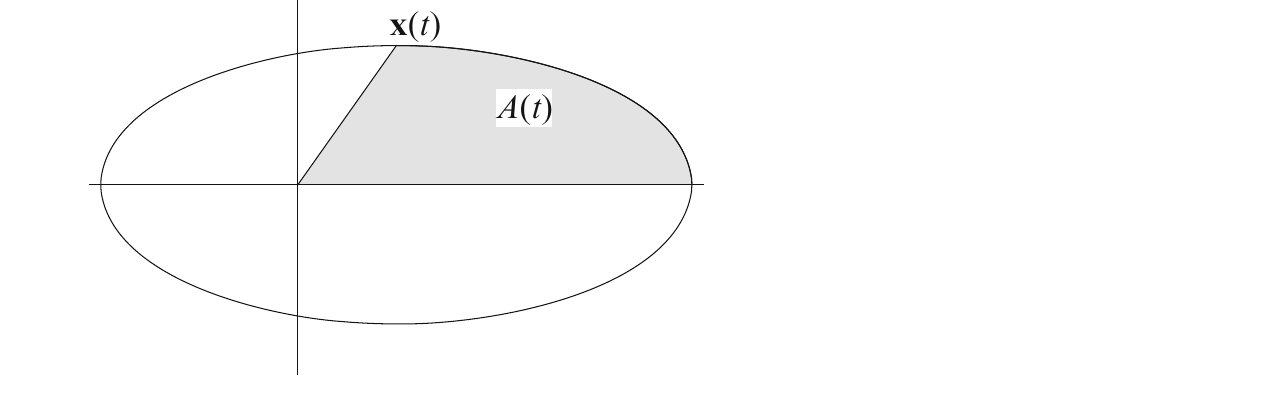
\includegraphics[width=.72\linewidth]{figures/figure-2-1.png}
  \caption{$A(t)$ 是阴影区域的面积.}\label{fig:angular-momentum-area}
\end{figure}

角动量的一个重要性质是:在某些情形下,它和能量一样是守恒的.

\begin{proposition}[旋转不变性与角动量]\label{pro:angular-momentum-conservation}
设质量为 $m$ 的粒子在 $\mathbb{R}^{2}$ 中运动,受势函数为 $V(x)$ 的保守力作用.如果 $V$ 在 $\mathbb{R}^{2}$ 的旋转下不变,那么沿牛顿方程的任意解,角动量 $J=x_{1}p_{2}-x_{2}p_{1}$ 都与时间无关.反过来,如果沿牛顿方程的每一条解,$J$ 都与时间无关,那么 $V$ 在旋转下不变.
\end{proposition}

\begin{proof}
沿一条解对式~\eqref{eq:angular-momentum-two-dimensional} 求导,得到
\begin{align*}
\frac{\mathrm{d}J}{\mathrm{d}t}
 &=\frac{\mathrm{d}x_{1}}{\mathrm{d}t}p_{2}+x_{1}\frac{\mathrm{d}p_{2}}{\mathrm{d}t}
  -\frac{\mathrm{d}x_{2}}{\mathrm{d}t}p_{1}-x_{2}\frac{\mathrm{d}p_{1}}{\mathrm{d}t}\\
 &=\frac1m p_{1}p_{2}-x_{1}\frac{\partial V}{\partial x_{2}}
  -\frac1m p_{2}p_{1}+x_{2}\frac{\partial V}{\partial x_{1}}\\
 &=x_{2}\frac{\partial V}{\partial x_{1}}-x_{1}\frac{\partial V}{\partial x_{2}}.
\end{align*}

另一方面,考虑 $\mathbb{R}^{2}$ 中的旋转 $R_{\theta}$:
\[
  R_{\theta}=\begin{pmatrix}
    \cos\theta&-\sin\theta\\
    \sin\theta&\cos\theta
  \end{pmatrix}.
\]
沿这族旋转对 $V$ 求导,可得
\[
\left.\frac{\mathrm{d}}{\mathrm{d}\theta}V(R_{\theta}x)\right|_{\theta=0}
=-x_{2}\frac{\partial V}{\partial x_{1}}+x_{1}\frac{\partial V}{\partial x_{2}}
=-\frac{\mathrm{d}J}{\mathrm{d}t}.
\]
因此,$V$ 的角向导数为零,当且仅当 $J$ 为常数.
\end{proof}

角动量的守恒结合关系式~\eqref{eq:angular-momentum-area},给出如下结果.

\begin{corollary}[Kepler 第二定律]\label{cor:kepler-second-law}
设粒子在 $\mathbb{R}^{2}$ 中运动,所受的力来自一个旋转不变的势函数.如果 $x(t)$ 是粒子的轨迹,那么在 $t=a$ 与 $t=b$ 之间,曲线 $x(t)$ 扫过的面积为
\[
  \frac{(b-a)J}{2m},
\]
其中 $J$ 是沿该轨迹恒定的角动量值.由于扫过的面积只依赖于 $b-a$,我们可以说:“相等的时间扫过相等的面积.”
\end{corollary}

当然,Kepler 研究的是在 $\mathbb{R}^{3}$ 中运动的行星,而不是 $\mathbb{R}^{2}$ 中的粒子.不过,在太阳的“平方反比”力作用下运动的行星,其运动总是位于某个平面内.(这个结论来自三维角动量守恒,见第~\ref{sec:kepler-problem} 节的说明.)

在 $\mathbb{R}^{3}$ 中,粒子的角动量是一个向量:
\begin{equation}
  J=x\times p,
  \label{eq:angular-momentum-three-dimensional}
\end{equation}
其中 $\times$ 表示叉积(或向量积).例如,
\begin{equation}
  J_{3}=x_{1}p_{2}-x_{2}p_{1}.
  \label{eq:angular-momentum-three-component}
\end{equation}
因此,如果一个 $\mathbb{R}^{3}$ 中的粒子恰好在 $\mathbb{R}^{2}$ 中运动(即 $x_{3}=0$ 且 $p_{3}=0$),那么角动量沿 $z$ 方向,其 $z$ 分量正是定义~\ref{def:angular-momentum} 中的量 $J$.

把 $\mathbb{R}^{3}$ 中粒子的角动量表示成向量,是低维空间中特有的现象.对于 $\mathbb{R}^{n}$ 中的粒子,角动量是一个斜对称矩阵:
\begin{equation}
  J_{jk}=x_{j}p_{k}-x_{k}p_{j}.
  \label{eq:angular-momentum-matrix}
\end{equation}
在 $\mathbb{R}^{3}$ 的情形,$3\times3$ 角动量矩阵的元素由角动量向量的三个分量及其负值组成,对角线上为零;可比较式~\eqref{eq:angular-momentum-three-component} 与~\eqref{eq:angular-momentum-matrix}.

\begin{definition}[系统的总角动量]\label{def:total-angular-momentum}
对于一个由 $N$ 个粒子组成、各粒子在 $\mathbb{R}^{n}$ 中运动的系统,总角动量是斜对称矩阵 $J$,其元素为
\begin{equation}
  J_{jk}=\sum_{l=1}^{N}\left(x^{l}_{j}p^{l}_{k}-x^{l}_{k}p^{l}_{j}\right).
  \label{eq:total-angular-momentum}
\end{equation}
\end{definition}

\begin{theorem}[总角动量守恒]\label{thm:total-angular-momentum}
设一个由 $N$ 个粒子组成、各粒子在 $\mathbb{R}^{n}$ 中运动的系统受到势函数为 $V$ 的保守力作用.如果对每个旋转矩阵 $R$ 都有
\begin{equation}
  V(Rx^{1},Rx^{2},\ldots,Rx^{N})=V(x^{1},x^{2},\ldots,x^{N}),
  \label{eq:rotation-invariance-many-particle}
\end{equation}
那么系统的总角动量守恒(沿每条轨迹为常数).反过来,如果总角动量沿每条轨迹都为常数,那么 $V$ 满足式~\eqref{eq:rotation-invariance-many-particle}.
\end{theorem}

这个结果的证明与命题~\ref{pro:angular-momentum-conservation} 的证明类似,留作练习(练习 10).下一节中,我们将用 Poisson 括号和 Hamilton 流的语言重新考察角动量的概念.

\section{Poisson 括号与 Hamilton 力学}

现在考虑经典力学的 Hamilton 处理方式.(此外还有 Lagrange 处理方式,但它与我们的目的不太相关.)Hamilton 处理方式,尤其是 Poisson 括号,将帮助我们理解守恒量的一般现象.Poisson 括号也是量子力学中使用对易子的一个重要动机来源.

在 Hamilton 处理方式中,我们把能量函数看成位置和动量的函数,而不是位置和速度的函数,并把它称为“Hamilton 函数”.如果 $\mathbb{R}^{n}$ 中的粒子具有通常的能量函数(动能加势能),则
\begin{equation}
  H(x,p)=\frac{1}{2m}\sum_{j=1}^{n}p_{j}^{2}+V(x).
  \label{eq:hamiltonian-one-particle}
\end{equation}
这里和通常一样,$p_{j}=m\dot{x}_{j}$.现在注意,牛顿定律可以写成
\begin{equation}
  \frac{\mathrm{d}x_{j}}{\mathrm{d}t}=\frac{\partial H}{\partial p_{j}},
  \qquad
  \frac{\mathrm{d}p_{j}}{\mathrm{d}t}=-\frac{\partial H}{\partial x_{j}}.
  \label{eq:hamilton-equations}
\end{equation}
事实上,对于形式~\eqref{eq:hamiltonian-one-particle} 的 $H$,这些方程给出 $\mathrm{d}x_{j}/\mathrm{d}t=p_{j}/m$,这正是 $p_{j}$ 的定义;同时 $\mathrm{d}p_{j}/\mathrm{d}t=-\partial V/\partial x_{j}=F_{j}$,这正是最初形式的牛顿定律.我们把形式~\eqref{eq:hamilton-equations} 的牛顿定律称为 Hamilton 方程.

虽然目前还不明显,把牛顿定律写成式~\eqref{eq:hamilton-equations} 的形式究竟带来了什么好处,但我们继续往下看.下一步是引入 Poisson 括号.

\begin{definition}[Poisson 括号]\label{def:poisson-bracket}
设 $f$ 和 $g$ 是 $\mathbb{R}^{2n}$ 上的两个光滑函数.把 $\mathbb{R}^{2n}$ 中的元素看成一对 $(x,p)$,其中 $x\in\mathbb{R}^{n}$ 表示粒子的位置,$p\in\mathbb{R}^{n}$ 表示粒子的动量.$f$ 与 $g$ 的 Poisson 括号记为 $\{f,g\}$,是 $\mathbb{R}^{2n}$ 上的函数,定义为
\begin{equation}
  \{f,g\}(x,p)=\sum_{j=1}^{n}\left(\frac{\partial f}{\partial x_{j}}\frac{\partial g}{\partial p_{j}}-\frac{\partial f}{\partial p_{j}}\frac{\partial g}{\partial x_{j}}\right).
  \label{eq:poisson-bracket}
\end{equation}
\end{definition}

Poisson 括号具有下列性质.

\begin{proposition}[Poisson 括号的性质]\label{pro:poisson-properties}
对 $\mathbb{R}^{2n}$ 上的任意光滑函数 $f,g,h$,有:
\begin{enumerate}
  \item 对任意 $c\in\mathbb{R}$,$\{f,g+ch\}=\{f,g\}+c\{f,h\}$;
  \item $\{g,f\}=-\{f,g\}$;
  \item $\{f,gh\}=\{f,g\}h+g\{f,h\}$;
  \item $\{f,\{g,h\}\}=\{\{f,g\},h\}+\{g,\{f,h\}\}$.
\end{enumerate}
\end{proposition}

命题~\ref{pro:poisson-properties} 的前两条性质说明 Poisson 括号是双线性的并且斜对称.第三条性质说明,“与 $f$ 作括号”这一运算相对于函数的逐点乘法满足导子性质(类似于导数的乘积法则);第四条性质则说明,“与 $f$ 作括号”相对于 Poisson 括号本身也满足导子性质.第四条性质等价于 Jacobi 恒等式
\begin{equation}
  \{f,\{g,h\}\}+\{h,\{f,g\}\}+\{g,\{h,f\}\}=0.
  \label{eq:poisson-jacobi}
\end{equation}
这可以利用 Poisson 括号的斜对称性直接验证.Jacobi 恒等式与双线性、斜对称性一起说明,$\mathbb{R}^{2n}$ 上的 $C^{\infty}$ 函数空间在 Poisson 括号运算下构成一个李代数(见第 16 章).

\begin{proof}
Poisson 括号的前两条性质显然成立,第三条是乘积法则的直接结果.我们说明如何直接计算第四条性质.(练习 15 给出了另一种证明.)计算可得
\[
\{f,\{g,h\}\}
=\sum_{j=1}^{n}\left[
\frac{\partial f}{\partial x_{j}}\frac{\partial}{\partial p_{j}}
  \left(\frac{\partial g}{\partial x_{j}}\frac{\partial h}{\partial p_{j}}-\frac{\partial g}{\partial p_{j}}\frac{\partial h}{\partial x_{j}}\right)
-\frac{\partial f}{\partial p_{j}}\frac{\partial}{\partial x_{j}}
  \left(\frac{\partial g}{\partial x_{j}}\frac{\partial h}{\partial p_{j}}-\frac{\partial g}{\partial p_{j}}\frac{\partial h}{\partial x_{j}}\right)
\right].
\]
例如,第一项使用乘积法则后会产生四项(这里及下文都对 $j$ 求和):
\begin{align}
&\frac{\partial f}{\partial x_{j}}\frac{\partial^{2}g}{\partial x_{j}\partial p_{j}}\frac{\partial h}{\partial p_{j}}
 +\frac{\partial f}{\partial x_{j}}\frac{\partial g}{\partial x_{j}}\frac{\partial^{2}h}{\partial p_{j}^{2}}
 -\frac{\partial f}{\partial x_{j}}\frac{\partial^{2}g}{\partial p_{j}^{2}}\frac{\partial h}{\partial x_{j}}
 -\frac{\partial f}{\partial x_{j}}\frac{\partial g}{\partial p_{j}}\frac{\partial^{2}h}{\partial x_{j}\partial p_{j}}.
\label{eq:poisson-proof-four-terms}
\end{align}
因此,式~\eqref{eq:poisson-jacobi} 左边总共有 24 项,每一项都对 $j$ 求和.每一项在三个函数中的两个函数上各有一个导数,在第三个函数上有两个导数.两阶导数落在哪个函数上共有三种可能;选定该函数后,另外两个函数上的导数有四种分配方式,而承担二阶导数的函数上的导数也随之确定(总共需要两个 $x$ 导数和两个 $p$ 导数).所以共有 12 种可能的项.直接而繁琐的检查表明,这 12 种项中的每一项都会在式~\eqref{eq:poisson-jacobi} 的左边出现两次,且符号相反.例如,在计算 $\{h,\{f,g\}\}$ 时,会得到一个与式~\eqref{eq:poisson-proof-four-terms} 的第二项类似的项,只需把 $(f,g,h)$ 换成 $(h,f,g)$:
\[
  \frac{\partial h}{\partial x_{j}}\frac{\partial f}{\partial x_{j}}\frac{\partial^{2}g}{\partial p_{j}^{2}}.
\]
这一项(出现在计算 $\{h,\{f,g\}\}$ 的过程中)恰好与式~\eqref{eq:poisson-proof-four-terms} 的第三项抵消(后者出现在计算 $\{f,\{g,h\}\}$ 的过程中).
\end{proof}

下面的初等结果将为量子力学中的“正则对易关系”提供有用的类比.

\begin{proposition}[位置与动量的 Poisson 括号]\label{pro:canonical-poisson-relations}
位置函数与动量函数满足
\[
  \{x_{j},x_{k}\}=0,\qquad
  \{p_{j},p_{k}\}=0,\qquad
  \{x_{j},p_{k}\}=\delta_{jk}.
\]
\end{proposition}

\begin{proof}
直接计算即可.
\end{proof}

考虑 Poisson 括号的另一个主要原因,是下面这个简单结果.

\begin{proposition}[沿 Hamilton 轨道的导数]\label{pro:derivative-poisson}
如果 $(x(t),p(t))$ 是 Hamilton 方程~\eqref{eq:hamilton-equations} 的一个解,那么对 $\mathbb{R}^{2n}$ 上任意光滑函数 $f$,都有
\begin{equation}
  \frac{\mathrm{d}}{\mathrm{d}t}f(x(t),p(t))=\{f,H\}(x(t),p(t)).
  \label{eq:derivative-poisson}
\end{equation}
\end{proposition}

通常把命题~\ref{pro:derivative-poisson} 更简洁地写成
\[
  \frac{\mathrm{d}f}{\mathrm{d}t}=\{f,H\},
\]
其中时间导数理解为沿某条轨迹的导数.

\begin{proof}
利用链式法则和 Hamilton 方程,
\begin{align*}
\frac{\mathrm{d}f}{\mathrm{d}t}
 &=\sum_{j=1}^{n}\left(\frac{\partial f}{\partial x_{j}}\frac{\mathrm{d}x_{j}}{\mathrm{d}t}+\frac{\partial f}{\partial p_{j}}\frac{\mathrm{d}p_{j}}{\mathrm{d}t}\right)\\
 &=\sum_{j=1}^{n}\left(\frac{\partial f}{\partial x_{j}}\frac{\partial H}{\partial p_{j}}-\frac{\partial f}{\partial p_{j}}\frac{\partial H}{\partial x_{j}}\right)\\
 &=\{f,H\},
\end{align*}
这正是所要证明的结论.
\end{proof}

注意,取 $f(x,p)=x_{j}$ 或 $f(x,p)=p_{j}$,命题~\ref{pro:derivative-poisson} 就包含了 Hamilton 方程本身.因此,这个命题给出了表达时间演化的一种与坐标无关的方式.

\begin{corollary}[守恒量与 Poisson 括号]\label{cor:poisson-conserved-quantity}
称 $\mathbb{R}^{2n}$ 上的光滑函数 $f$ 是一个守恒量,如果对 Hamilton 方程的每条解 $(x(t),p(t))$,$f(x(t),p(t))$ 都与 $t$ 无关.那么 $f$ 是守恒量,当且仅当
\[
  \{f,H\}=0.
\]
特别地,Hamilton 函数 $H$ 是守恒量.
\end{corollary}

守恒量也称为运动常数.关于这个结果的另一种观点,见结论 2.31.守恒量(如果能够找到)很有用,因为我们知道轨迹必须位于每个守恒量的等值面内.例如,设粒子在 $\mathbb{R}^{2}$ 中运动,Hamilton 函数 $H$ 和另一个独立函数 $f$(比如角动量)都是守恒量.那么我们不必在四维相空间中寻找轨迹,而只需在 $H$ 和 $f$ 的联合等值集内寻找轨迹,即寻找形如 $H(x,p)=a$、$f(x,p)=b$(其中 $a,b$ 是常数)的集合.这些联合等值集通常是二维的,而不是四维的,因此守恒量把问题从四个变量的方程大幅简化成了两个变量的方程.

在 $\mathbb{R}^{2n}$ 上求解 Hamilton 方程,会产生一个流,即一族 $\mathbb{R}^{2n}$ 的微分同胚 $\Phi_{t}$;其中 $\Phi_{t}(x,p)$ 等于以 $(x,p)$ 为初始条件的 Hamilton 方程在时间 $t$ 的解.根据势函数 $V$ 的选择,粒子可能在有限时间内逃到无穷远,因此映射 $\Phi_{t}$ 不一定在整个 $\mathbb{R}^{2n}$ 上有定义,而可能只在其中某个开子集上有定义.如果 $\Phi_{t}$ 对所有 $t$ 都在整个 $\mathbb{R}^{2n}$ 上有定义,我们就称这个流是\emph{完备的}.

\begin{theorem}[Liouville 定理]\label{thm:liouville}
任意 Hamilton 函数 $H$ 的 Hamilton 方程所对应的流,都保持 $(2n)$ 维体积测度
\[
  \mathrm{d}x_{1}\,\mathrm{d}x_{2}\cdots\mathrm{d}x_{n}\,\mathrm{d}p_{1}\,\mathrm{d}p_{2}\cdots\mathrm{d}p_{n}
\]
不变.

更准确地说,如果可测集 $E$ 对某个 $t\in\mathbb{R}$ 包含在 $\Phi_{t}$ 的定义域中,那么 $\Phi_{t}(E)$ 的体积等于 $E$ 的体积.
\end{theorem}

\begin{proof}
Hamilton 方程可以写成
\begin{equation}
\frac{\mathrm{d}}{\mathrm{d}t}
\begin{pmatrix}
 x_{1}\\ \vdots\\ x_{n}\\ p_{1}\\ \vdots\\ p_{n}
\end{pmatrix}
=
\begin{pmatrix}
 \partial H/\partial p_{1}\\ \vdots\\ \partial H/\partial p_{n}\\
 -\partial H/\partial x_{1}\\ \vdots\\ -\partial H/\partial x_{n}
\end{pmatrix}.
\label{eq:hamilton-vector-field}
\end{equation}
这意味着 Hamilton 方程描述了 $\mathbb{R}^{2n}$ 上沿式~\eqref{eq:hamilton-vector-field} 右端向量场的流.向量分析的一个标准结果(例如见 [29] 中的命题 16.33)表明,当且仅当该向量场的散度为零时,这个流保持体积.我们计算散度得到
\[
  \frac{\partial}{\partial x_{1}}\frac{\partial H}{\partial p_{1}}+\cdots+\frac{\partial}{\partial x_{n}}\frac{\partial H}{\partial p_{n}}
  -\frac{\partial}{\partial p_{1}}\frac{\partial H}{\partial x_{1}}-\cdots-\frac{\partial}{\partial p_{n}}\frac{\partial H}{\partial x_{n}}.
\]
由于
\[
  \frac{\partial^{2}H}{\partial x_{j}\partial p_{j}}
  =\frac{\partial^{2}H}{\partial p_{j}\partial x_{j}},
\]
所以散度为零.
\end{proof}

不变体积的存在对系统动力学有重要后果.例如,对于“受限”系统,不变体积意味着系统表现出“回归性”:粗略地说,对大多数初始条件,粒子最终都会在相空间中任意接近其初始状态.不过,我们不在这里深入讨论这一点.

注意,式~\eqref{eq:hamilton-vector-field} 中计算出的 $X_{H}$ 的散度以一种非常特殊的方式为零,即第 $j$ 项与第 $(n+j)$ 项对每个 $1\leq j\leq n$ 都分别抵消.事实证明,这个更强的条件等价于:任意 $\mathbb{R}^{2n}$ 上的光滑函数所对应的 Hamilton 流 $\Phi_{t}$ 保持辛形式 $\omega$ 不变,其中
\[
  \omega\bigl((x,p),(x',p')\bigr)=x\cdot p'-p\cdot x'.
\]
更准确地说,对任意 $t\in\mathbb{R}$ 和任意 $(x,p)\in\mathbb{R}^{2n}$,把 $\Phi_{t}$ 在 $(x,p)$ 处的偏导数矩阵看成从 $\mathbb{R}^{2n}$ 到 $\mathbb{R}^{2n}$ 的线性映射,它保持 $\omega$ 不变.事实证明,$\Phi_{t}$ 的这一性质等价于它保持 Poisson 括号,即对所有 $f,g\in C^{\infty}(\mathbb{R}^{n})$,
\[
  \{f\circ\Phi_{t},g\circ\Phi_{t}\}=\{f,g\}\circ\Phi_{t}.
\]
保持 $\omega$ 的映射 $\Psi:\mathbb{R}^{2n}\to\mathbb{R}^{2n}$ 在数学记号中称为辛同胚,在物理学记号中称为正则变换.我们把这些结论的证明推迟到第 21 章,到那时我们将在更一般的情形下讨论它们.

\begin{definition}[Hamilton 流的生成元]\label{def:hamiltonian-generator}
对 $\mathbb{R}^{2n}$ 上的任意光滑函数 $f$,把 Hamilton 方程~\eqref{eq:hamilton-equations} 中的 Hamilton 函数 $H$ 换成 $f$,求解所得的流称为由 $f$ 生成的 Hamilton 流;函数 $f$ 称为相应流的 Hamilton 生成元.
\end{definition}

虽然任意光滑函数都可以代入 Hamilton 方程以产生一个流,但从物理上看,应当认为系统有一个特殊的函数,即系统的 Hamilton 函数 $H$,由 $H$ 生成的流才是系统的时间演化.对于其他函数 $f$,由 $f$ 生成的 Hamilton 流不应被理解为时间演化,而应理解为某种其他的流,例如它可能表示系统的一族对称性.

\begin{proposition}[平移的 Hamilton 流]\label{pro:hamiltonian-translations}
函数
\begin{equation}
  f_{a}(x,p):=a\cdot p
  \label{eq:hamiltonian-position-translation}
\end{equation}
生成的 Hamilton 流为
\begin{equation}
  x(t)=x_{0}+ta,\qquad p(t)=p_{0}.
  \label{eq:hamiltonian-position-translation-flow}
\end{equation}
函数
\begin{equation}
  g_{b}(x,p):=b\cdot x
  \label{eq:hamiltonian-momentum-translation}
\end{equation}
生成的 Hamilton 流为
\[
  x(t)=x_{0},\qquad p(t)=p_{0}-tb.
\]
\end{proposition}

\begin{proof}
直接计算即可.
\end{proof}

这意味着,由动量函数的线性组合生成的 Hamilton 流,是对粒子位置作平移.也就是说,在式~\eqref{eq:hamiltonian-position-translation} 中由 $f_{a}$ 生成的流~\eqref{eq:hamiltonian-position-translation-flow} 中,粒子的初始位置 $x_{0}$ 被平移了 $ta$,而粒子的动量与 $t$ 无关.同样地,由位置函数的线性组合(函数 $g_{b}$)生成的 Hamilton 流,是对粒子动量作平移.

\begin{proposition}[角动量生成旋转]\label{pro:angular-momentum-flow}
对一个在 $\mathbb{R}^{2}$ 中运动的粒子,角动量函数
\[
  J(x,p)=x_{1}p_{2}-x_{2}p_{1}
\]
所生成的 Hamilton 流由 $x$ 和 $p$ 的同时旋转组成,即
\begin{equation}
  \begin{pmatrix}x_{1}(t)\\x_{2}(t)\end{pmatrix}
  =\begin{pmatrix}\cos t&-\sin t\\\sin t&\cos t\end{pmatrix}
   \begin{pmatrix}x_{1}(0)\\x_{2}(0)\end{pmatrix},
  \qquad
  \begin{pmatrix}p_{1}(t)\\p_{2}(t)\end{pmatrix}
  =\begin{pmatrix}\cos t&-\sin t\\\sin t&\cos t\end{pmatrix}
   \begin{pmatrix}p_{1}(0)\\p_{2}(0)\end{pmatrix}.
  \label{eq:angular-momentum-hamiltonian-flow}
\end{equation}
\end{proposition}

\begin{proof}
将角动量函数 $J$ 代替 Hamilton 方程中的 $H$,得到
\[
  \frac{\mathrm{d}x_{1}}{\mathrm{d}t}=\frac{\partial J}{\partial p_{1}}=-x_{2},
  \qquad
  \frac{\mathrm{d}p_{1}}{\mathrm{d}t}=-\frac{\partial J}{\partial x_{1}}=-p_{2},
\]
\[
  \frac{\mathrm{d}x_{2}}{\mathrm{d}t}=\frac{\partial J}{\partial p_{2}}=x_{1},
  \qquad
  \frac{\mathrm{d}p_{2}}{\mathrm{d}t}=-\frac{\partial J}{\partial x_{2}}=p_{1}.
\]
这个系统的解由式~\eqref{eq:angular-momentum-hamiltonian-flow} 给出,直接求导即可验证.
\end{proof}

注意,由 $J$ 生成的 Hamilton 流并不具有粒子时间演化的解释,所以式~\eqref{eq:angular-momentum-hamiltonian-flow} 中的参数 $t$ 不应解释为物理时间;它只是一个一参数微分同胚群中的参数.在这里,$t$ 是旋转角.因此,对“角动量是什么？”这个问题,一个答案是:$J$ 是旋转的 Hamilton 生成元.

如果 $f$ 是任意光滑函数,那么根据命题~\ref{pro:derivative-poisson} 的证明,沿由 $f$ 生成的 Hamilton 流,另一个函数 $g$ 的时间导数为 $\mathrm{d}g/\mathrm{d}t=\{g,f\}$.特别地,Hamilton 函数 $H$ 沿由 $f$ 生成的流的导数是 $\{H,f\}$.因此,$f$ 沿由 $H$ 生成的流为常数,当且仅当 $\{f,H\}=0$;这又当且仅当 $H$ 沿由 $f$ 生成的流为常数.这个推理给出如下结论.

\begin{conclusion}
函数 $f$ 对 Hamilton 方程~\eqref{eq:hamilton-equations} 的解来说是守恒量,当且仅当 $H$ 在由 $f$ 生成的 Hamilton 流下不变.特别地,角动量 $J$ 守恒,当且仅当 $H$ 在 $x$ 和 $p$ 的同时旋转下不变.
\end{conclusion}

我们将在第 21 章回到这种理解守恒量的方式.另见练习 12.

Hamilton 框架可以直接推广到粒子系统.

\begin{proposition}[多粒子 Hamilton 系统]\label{pro:many-particle-hamiltonian}
考虑一个由 $N$ 个粒子组成、各粒子在 $\mathbb{R}^{n}$ 中运动的系统,其相空间为 $\mathbb{R}^{2nN}$,可以看成形如
\[
  (x^{1},\ldots,x^{N},p^{1},\ldots,p^{N})
\]
的 $(2N)$ 元组所成的集合,其中 $x^{j},p^{j}\in\mathbb{R}^{n}$.在相空间上,对两个光滑函数 $f,g$ 定义 Poisson 括号
\[
  \{f,g\}=\sum_{j=1}^{N}\sum_{k=1}^{n}\left(
  \frac{\partial f}{\partial x^{j}_{k}}\frac{\partial g}{\partial p^{j}_{k}}
  -\frac{\partial f}{\partial p^{j}_{k}}\frac{\partial g}{\partial x^{j}_{k}}\right),
\]
并考虑形式为
\[
  H(x^{1},\ldots,x^{N},p^{1},\ldots,p^{N})
  =\sum_{j=1}^{N}\frac{1}{2m_{j}}\lvert p^{j}\rvert^{2}+V(x^{1},\ldots,x^{N})
\]
的 Hamilton 函数.那么,形式为 $m_{j}\ddot{x}^{j}=-\nabla_{j}V$ 的牛顿定律等价于 Hamilton 方程
\begin{equation}
  \frac{\mathrm{d}x^{j}_{k}}{\mathrm{d}t}=\frac{\partial H}{\partial p^{j}_{k}},
  \qquad
  \frac{\mathrm{d}p^{j}_{k}}{\mathrm{d}t}=-\frac{\partial H}{\partial x^{j}_{k}}.
  \label{eq:many-particle-hamilton-equations}
\end{equation}
对 Hamilton 方程的任意解和任意光滑函数 $f$,都有
\[
  \frac{\mathrm{d}f}{\mathrm{d}t}=\{f,H\}.
\]
\end{proposition}

这个结果的证明与单粒子情形完全类似,故略去.

\section{Kepler 问题与 Runge--Lenz 向量}\label{sec:kepler-problem}

\subsection{Kepler 问题}\label{subsec:kepler-problem}

现在考虑经典的 Kepler 问题,即寻找行星绕太阳运动的轨迹.由于太阳的质量远大于任何一颗行星,我们可以把太阳的位置看成固定在坐标系原点.太阳对行星施加的力为
\begin{equation}
  F=-k\frac{x}{\lvert x\rvert^{3}},
  \label{eq:kepler-force}
\end{equation}
其中 $k=GmM$,$m$ 是行星质量,$M$ 是太阳质量,$G$ 是万有引力常数.注意,$F$ 的大小与到原点距离的平方的倒数成正比,因此这个力满足平方反比定律.由于 $k$ 含有行星质量 $m$ 这一因子,而运动方程是 $m\ddot{x}=F$,所以 $m$ 会从运动方程中约掉.与力~\eqref{eq:kepler-force} 对应的势能显然是
\begin{equation}
  V(x)=-\frac{k}{\lvert x\rvert}.
  \label{eq:kepler-potential}
\end{equation}

由于势能 $V$ 在旋转下不变,角动量向量 $J=x\times p$ 是守恒量(定理~\ref{thm:total-angular-momentum},取 $N=1$、$n=3$).如果 $J=0$,粒子沿着经过原点的一条射线运动.在这种情况下,如果初始动量指向原点,粒子将在未来某时刻穿过原点;如果初始动量背离原点,则粒子必定在过去某时刻穿过原点.这类轨迹称为\emph{碰撞轨迹},我们将把它们视为病态情形.

从现在开始,我们只考虑角动量向量非零的轨迹.固定粒子的能量和角动量,会保证粒子始终与原点保持某个最小距离(见练习 20).另一方面,由于 $J=x\times p$,粒子的位置 $x(t)$ 始终垂直于 $J$ 的恒定值.因此,我们把经过原点且垂直于 $J$ 的平面称为\emph{运动平面}.

\subsection{Runge--Lenz 向量的守恒}

我们将借助一个称为 Runge--Lenz 向量的对象,以间接方式描述经典轨迹.

\begin{definition}[Runge--Lenz 向量]\label{def:runge-lenz-vector}
Runge--Lenz 向量是在 $(\mathbb{R}^{3}\setminus\{0\})\times\mathbb{R}^{3}$ 上取向量值的函数,定义为
\begin{equation}
  A(x,p)=\frac{1}{mk}\,p\times J-\frac{x}{\lvert x\rvert}.
  \label{eq:runge-lenz-vector}
\end{equation}
这里 $x$ 表示经典粒子的位置,$p$ 表示其动量.
\end{definition}

这个向量的重要性在于:对于 Kepler 问题,它是一个守恒量.当然,只要势能是径向的(即距离原点的函数),角动量向量就是守恒量.Kepler 问题中形如 $1/r$ 的势能之所以特殊,是因为它还有另一个守恒的向量值量.

\begin{proposition}[Runge--Lenz 向量守恒]\label{pro:runge-lenz-conservation}
对受力~\eqref{eq:kepler-force} 作用而满足 Newton 定律的粒子,Runge--Lenz 向量是守恒量.
\end{proposition}

\begin{proof}
由于 $J$ 守恒,我们计算得到
\begin{align*}
\dot{A}(t)
 &=\frac{1}{mk}F\times J-\frac{1}{m}\frac{\mathrm{d}}{\mathrm{d}t}\left(\frac{x}{\lvert x\rvert}\right)\\
 &=-\frac{1}{m\lvert x\rvert^{3}}x\times(x\times p)-\frac{1}{m}\left(\frac{p}{\lvert x\rvert}-\frac{x(x\cdot p)}{\lvert x\rvert^{3}}\right)\\
 &=\frac1m\left[-\frac{x(x\cdot p)}{\lvert x\rvert^{3}}+\frac{p(x\cdot x)}{\lvert x\rvert^{3}}-\frac{p}{\lvert x\rvert}+\frac{x(x\cdot p)}{\lvert x\rvert^{3}}\right]\\
 &=0.
\end{align*}
这里使用了对所有 $b,c,d\in\mathbb{R}^{3}$ 都成立的恒等式
\[
  b\times(c\times d)=c(b\cdot d)-d(b\cdot c).
\]
\end{proof}

\subsection{椭圆、双曲线和抛物线}

现在利用 Runge--Lenz 向量确定 Kepler 问题的轨迹.

\begin{proposition}[Runge--Lenz 向量的大小]\label{pro:runge-lenz-magnitude}
Runge--Lenz 向量 $A$ 的大小满足
\begin{equation}
  \lvert A\rvert^{2}=1+\frac{2\lvert J\rvert^{2}}{mk^{2}}E,
  \label{eq:runge-lenz-magnitude}
\end{equation}
其中 $E=\lvert p\rvert^{2}/(2m)-k/\lvert x\rvert$ 是粒子的能量.此外,如果 $\widehat{x}:=x/\lvert x\rvert$ 是 $x$ 方向上的单位向量,那么对所有非零 $x$ 都有
\begin{equation}
  A\cdot\widehat{x}=\frac{\lvert J\rvert^{2}}{mk\lvert x\rvert}-1.
  \label{eq:runge-lenz-radial-relation}
\end{equation}
由此得到
\begin{equation}
  \lvert x\rvert=\frac{\lvert J\rvert^{2}}{mk(1+A\cdot\widehat{x})}.
  \label{eq:kepler-radial-equation}
\end{equation}
注意,从式~\eqref{eq:runge-lenz-radial-relation} 可知,对所有 $x\neq0$,都有 $A\cdot\widehat{x}>-1$.
\end{proposition}

\begin{proof}
利用恒等式 $b\cdot(c\times d)=d\cdot(b\times c)$,可得
\[
  \widehat{x}\cdot(p\times J)=J\cdot(\widehat{x}\times p)=\frac{\lvert J\rvert^{2}}{\lvert x\rvert}.
\]
由于 $J$ 与 $p$ 正交,
\begin{align*}
\lvert A\rvert^{2}
 &=\frac{1}{m^{2}k^{2}}\lvert p\rvert^{2}\lvert J\rvert^{2}+1-\frac{2}{mk}\widehat{x}\cdot(p\times J)\\
 &=1+\frac{2\lvert J\rvert^{2}}{mk}\left(\frac{\lvert p\rvert^{2}}{2m}-\frac{k}{\lvert x\rvert}\right)\\
 &=1+\frac{2\lvert J\rvert^{2}}{mk^{2}}E.
\end{align*}
再次使用 $b\cdot(c\times d)=d\cdot(b\times c)$,得到
\[
  A\cdot x=\frac{1}{mk}J\cdot(x\times p)-\frac{x\cdot x}{\lvert x\rvert}
  =\frac{\lvert J\rvert^{2}}{mk}-\lvert x\rvert.
\]
两边除以 $\lvert x\rvert$,便得到 $A\cdot\widehat{x}$ 的表达式;再解出 $\lvert x\rvert$ 即得结论.
\end{proof}

\begin{corollary}[Kepler 轨道的极坐标方程]\label{cor:kepler-polar-equation}
在运动平面内选取一组正交坐标,使 $A$ 沿正 $x_{1}$ 轴方向.若 $(r,\theta)$ 是与这组坐标对应的极坐标,那么沿每条轨迹 $(r(t),\theta(t))$ 都有
\begin{equation}
  r(t)=\frac{\lvert J\rvert^{2}}{mk\bigl(1+A\cos\theta(t)\bigr)},
  \label{eq:kepler-polar-orbit}
\end{equation}
其中 $A=\lvert A\rvert$.如果 $A=0$,则可以使用任意正交坐标.
\end{corollary}

\begin{proposition}[Kepler 轨道的类型]\label{pro:kepler-orbit-types}
如果 $A:=\lvert A\rvert<1$,则式~\eqref{eq:kepler-polar-orbit} 是一条离心率为 $A$、且原点为其一个焦点的椭圆方程.如果 $A>1$,它是双曲线方程;如果 $A=1$,它是抛物线方程.

粒子在运动平面内的轨道,在粒子能量为负时是椭圆,在能量为正时是双曲线,在能量为零时是抛物线.
\end{proposition}

\begin{figure}[htbp]
  \centering
  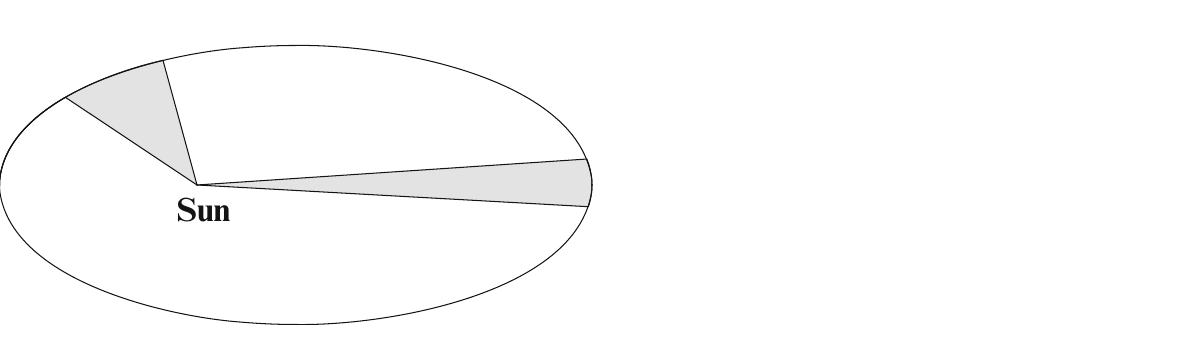
\includegraphics[width=.70\linewidth]{figures/figure-2-2.png}
  \caption{Kepler 问题中的椭圆轨道,阴影部分为两个相等的面积.}\label{fig:kepler-ellipse}
\end{figure}

Kepler 第一定律断言,行星沿椭圆轨道运动,太阳位于其中一个焦点,如图~\ref{fig:kepler-ellipse} 所示.阴影区域表示在相等时间内扫过的两个相等面积,这与 Kepler 第二定律(推论~\ref{cor:kepler-second-law})一致.

回忆一下,椭圆的离心率为 $\sqrt{1-(b/a)^{2}}$,其中 $a$ 是长轴长度的一半,$b$ 是短轴长度的一半.因此,当 $A=0$ 时,$b=a$,椭圆就是圆.

\begin{proof}
继续在 $A$ 沿正 $x_{1}$ 轴方向的坐标系中工作.此时式~\eqref{eq:kepler-polar-orbit} 变为
\[
  \sqrt{x^{2}+y^{2}}=\alpha\frac{1}{1+A\dfrac{x}{\sqrt{x^{2}+y^{2}}}},
\]
其中 $\alpha=\lvert J\rvert^{2}/(mk)$.由此得到
\[
  1=\frac1\alpha\left(\sqrt{x^{2}+y^{2}}+Ax\right).
\]
现在解出 $\sqrt{x^{2}+y^{2}}$,将方程两边平方并化简.假设 $A^{2}\neq1$,可得
\begin{equation}
  \alpha^{2}\left(\frac{1}{1-A^{2}}\right)
  =(1-A^{2})\left(x+\frac{A\alpha}{1-A^{2}}\right)^{2}+y^{2}.
  \label{eq:kepler-conic-equation}
\end{equation}
这是椭圆(若 $A^{2}<1$)或双曲线(若 $A^{2}>1$)的方程,其中心为 $(-\alpha/(1-A^{2}),0)$.结合命题~\ref{pro:runge-lenz-magnitude} 中关于 $A:=\lvert A\rvert$ 的公式,可知粒子能量为负时得到椭圆,能量为正时得到双曲线.

当 $A^{2}<1$ 时,可以直接计算出椭圆长轴和短轴的半长分别为
\[
  a=\frac{\alpha}{1-A^{2}},
  \qquad
  b=\frac{\alpha}{\sqrt{1-A^{2}}}.
\]
由此容易算出离心率为 $A$.椭圆两焦点之间的距离等于长轴长度乘以离心率,在这里为 $2A\alpha/(1-A^{2})$.由于式~\eqref{eq:kepler-conic-equation} 中椭圆的中心是 $( -A\alpha/(1-A^{2}),0)$,原点正好是椭圆的一个焦点.

如果 $A^{2}=1$,进行同样的分析时,$x^{2}$ 项会从方程中消失,得到
\[
  x=\frac{1}{2A\alpha}\left(-y^{2}+\alpha^{2}\right),
\]
这是沿 $x$ 轴开口的抛物线方程.这种情形对应于能量为零.
\end{proof}

注意,命题~\ref{pro:kepler-orbit-types} 没有告诉我们粒子作为时间函数如何沿椭圆、双曲线或抛物线运动.不过,原则上可以利用角动量确定这一点.事实上,在运动平面中应用式~\eqref{eq:angular-momentum-polar},得到
\begin{equation}
  \frac{\mathrm{d}\theta}{\mathrm{d}t}=\frac{1}{mr^{2}}\lvert J\rvert,
  \label{eq:kepler-angular-speed}
\end{equation}
其中 $\theta$ 是运动平面内的极角变量.由于推论~\ref{cor:kepler-polar-equation} 已经给出了 $r$ 关于 $\theta$ 的函数关系,式~\eqref{eq:kepler-angular-speed} 给出一个(一阶、可分离变量的)微分方程;我们可以尝试求解它,从而得到 $\theta$——以及 $r$——关于 $t$ 的函数.

\subsection{Kepler 问题的特殊性质}

如前所述,除了守恒的能量和角动量之外,还存在另一个守恒的向量值函数,这是势能取 $-k/\lvert x\rvert$ 形式所特有的.对于一般的径向势能,能量和角动量将是仅有的守恒量.假设 $J\neq0$,任意径向势能中的粒子运动总是位于垂直于 $J$ 的平面内.考虑到这一点,我们可以把粒子看成在 $\mathbb{R}^{2}$ 而不是 $\mathbb{R}^{3}$ 中运动,并相应地把相空间看成四维而不是六维.从这个角度看,还剩下两个守恒量,即能量 $E$ 和运动平面中的标量角动量 $J$(如定义~\ref{def:angular-momentum} 所给出).因此,每条轨迹都位于形如
\[
  \left\{(x,p)\in\mathbb{R}^{2}\times\mathbb{R}^{2}:E(x,p)=a,\ J(x,p)=b\right\}
\]
的集合中.这种集合称为 $E$ 与 $J$ 的\emph{联合等值集}.这些集合是四维相空间中的二维曲面.

对于一般的径向势能,相空间中的轨迹 $(x(t),p(t))$ 可能不是一条闭曲线,而是在它所在的联合等值面中填满一个稠密子集.特别地,位置空间中的轨迹 $x(t)$ 通常不是闭曲线.例如,$x(t)$ 可能在运动平面内描出一个大致椭圆形的区域,但椭圆的轴会发生“进动”,也就是随时间变化.图~\ref{fig:radial-potential-precession} 展示了这样一条轨迹;应将它与图~\ref{fig:kepler-ellipse} 对照.

\begin{figure}[htbp]
  \centering
  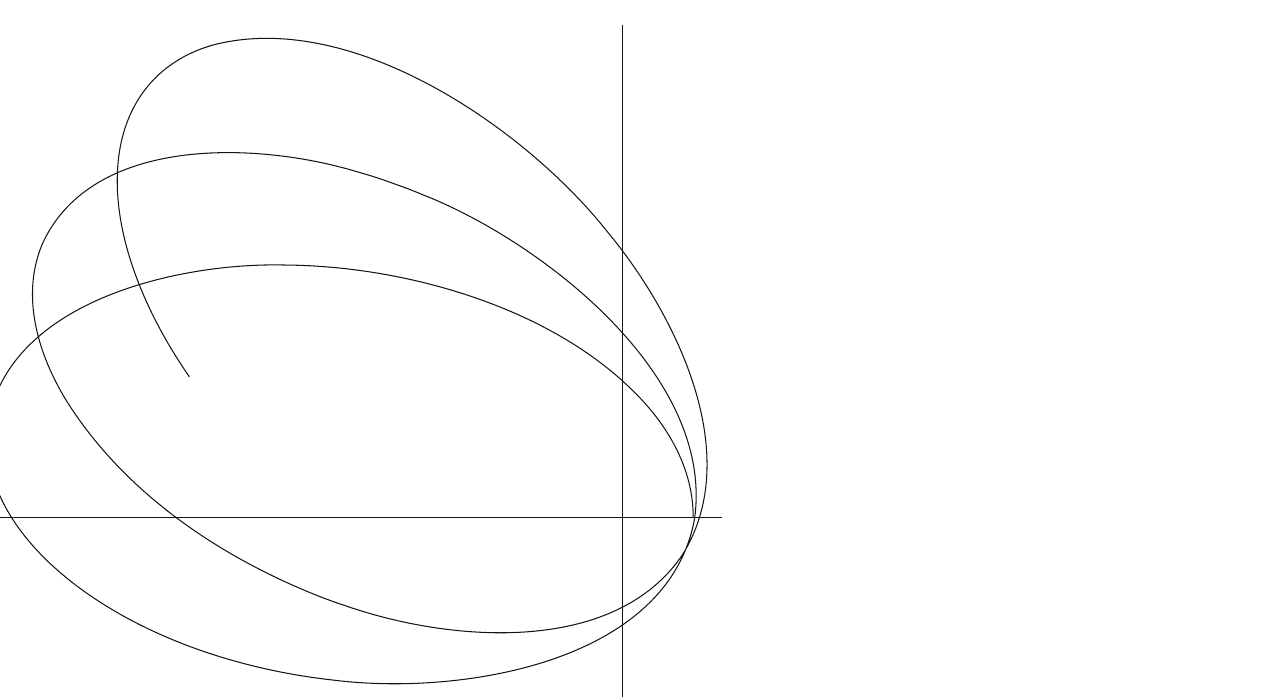
\includegraphics[width=.70\linewidth]{figures/figure-2-3.png}
  \caption{典型径向势能下,运动平面内的轨迹.}\label{fig:radial-potential-precession}
\end{figure}

在 Kepler 问题中,即使把注意力限制在运动平面内,除了 $E$ 和 $J$ 之外仍有一个守恒量,即 $A$ 的方向;它可以用运动平面内 $A$ 与 $x_{1}$ 轴之间的角度 $\phi$ 表示.(注意,$A$ 的定义中的两项都位于运动平面内;还要注意,根据命题~\ref{pro:runge-lenz-magnitude},$A$ 的大小可以由 $E$ 和 $J$ 计算出来.)因此,Kepler 问题的轨迹位于 $E$、$J$ 和 $\phi$ 的联合等值集中,这些集合是一维的.当 $E<0$ 时,$E$ 和 $J$ 的联合等值集是紧的;此时 $E$、$J$ 和 $\phi$ 的联合等值集也是紧的一维集合,也就是简单闭曲线.

Kepler 问题的另一个特殊性质是:所有具有相同能量的轨迹(即能量为负的闭轨道)具有相同的周期(见练习 21).这种表面上的巧合可以通过证明由 $J$ 和 $A$ 生成的 Hamilton 流在能量曲面上传递作用来解释.这些流与系统的时间演化相交换,因为它们都是守恒量(结论 2.31).因此,具有相同能量的任意两个点对于时间演化来说都是“等价的”.我们不在这里展开这一分析的细节,但将在第 18.4 节更好地理解由 $A$ 的各分量生成的流.

\section{练习}

\begin{exercise}\label{ex:travel-time}
考虑一个在实轴上运动的粒子,它所受的力来自势函数 $V$.给定粒子的某个能量值 $E_{0}$,假设在某个闭区间 $[x_{0},x_{1}]$ 内处处有 $V(x)<E_{0}$.若粒子的初始位置为 $x_{0}$ 且初始速度为正,那么它将一直向右运动,直到到达 $x_{1}$.利用式~\eqref{eq:energy-first-integral},证明粒子从 $x_{0}$ 运动到 $x_{1}$ 所需的时间为
\[
  t=\int_{x_{0}}^{x_{1}}\sqrt{\frac{m}{2(E_{0}-V(y))}}\,\mathrm{d}y.
\]
\begin{note}
这说明,对于 $\mathbb{R}^{1}$ 中的牛顿方程,我们或多或少可以显式地求出时间关于位置的函数;原则上,这就确定了位置关于时间的函数.
\end{note}
\end{exercise}

\begin{exercise}\label{ex:xp-flow}
求 $\mathbb{R}^{2}$ 上由函数
\[
  f(x,p)=xp
\]
生成的 Hamilton 流.
\end{exercise}

\begin{exercise}\label{ex:angular-poisson-algebra}
令 $J$ 表示在 $\mathbb{R}^{3}$ 中运动的粒子的角动量向量,即 $J=x\times p$.证明 $J$ 的三个分量满足下列 Poisson 括号关系:
\[
  \{J_{1},J_{2}\}=J_{3},\qquad
  \{J_{2},J_{3}\}=J_{1},\qquad
  \{J_{3},J_{1}\}=J_{2}.
\]
\end{exercise}

\begin{exercise}\label{ex:kepler-minimum-radius}
在 Kepler 问题中,证明对每个实数 $E$ 和正数 $J$,都存在 $\varepsilon>0$,使得对所有满足 $E(x,p)=E$ 且 $\lvert J(x,p)\rvert=J$ 的 $(x,p)$,都有 $\lvert x\rvert\geq\varepsilon$.
\begin{note}
提示:假设 $(x_{n},p_{n})$ 是满足 $\lvert J(x_{n},p_{n})\rvert=J$ 的序列,且 $\lvert x_{n}\rvert$ 趋于零.证明 $E(x_{n},p_{n})$ 趋于 $+\infty$.
\end{note}
\end{exercise}

\begin{exercise}\label{ex:kepler-period}
\begin{enumerate}[label=(\alph*)]
  \item 在命题~\ref{pro:kepler-orbit-types} 中的运动平面内,且在 $A<1$ 的情形下,求椭圆的面积.
  \item 证明粒子沿椭圆完整运行一周所需的时间 $T$ 为
  \[
    T=\frac{\pi}{\sqrt{2}}GM(-\widetilde{E})^{-3/2},
  \]
  其中 $\widetilde{E}$ 是粒子的“无质量能量”,定义为
  \[
    \widetilde{E}=\frac{E}{m}=\frac12\lvert\dot{x}\rvert^{2}-\frac{GM}{\lvert x\rvert}.
  \]
\end{enumerate}
\begin{note}
在轨迹位于运动平面内的椭圆情形,粒子的能量为负.第 (b) 部分的结果与 Kepler 第三定律密切相关.
\end{note}
\end{exercise}

\begin{exercise}\label{ex:vector-field-commutator}
令 $X$ 和 $Y$ 是 $\mathbb{R}^{n}$ 上的“向量场”,并把它们看成一阶微分算子,即
\[
  X=\sum_{j=1}^{n}a_{j}(x)\frac{\partial}{\partial x_{j}},
  \qquad
  Y=\sum_{j=1}^{n}b_{j}(x)\frac{\partial}{\partial x_{j}}.
\]
(如果 $\widetilde{X}(x)=(a_{1}(x),\ldots,a_{n}(x))$,那么算子 $X$ 是沿 $\widetilde{X}$ 方向的方向导数.通常把向量值函数 $\widetilde{X}$ 与相应的一阶微分算子 $X$ 视为同一个对象.)证明由
\[
  [X,Y]=XY-YX
\]
定义的交换子 $[X,Y]$ 仍然是一个向量场,即一个一阶微分算子.
\end{exercise}

\begin{exercise}\label{ex:hamiltonian-vector-field}
回忆练习~\ref{ex:vector-field-commutator} 之前对 Hamilton 向量场 $X_{f}$ 的定义.对 $\mathbb{R}^{2n}$ 上的光滑函数 $f$,定义作用在 $C^{\infty}(\mathbb{R}^{2n})$ 上的算子 $X_{f}$:
\[
  X_{f}(g)=\{f,g\}.
\]
也就是说,
\[
  X_{f}=\sum_{j=1}^{n}\left(
  \frac{\partial f}{\partial x_{j}}\frac{\partial}{\partial p_{j}}
  -\frac{\partial f}{\partial p_{j}}\frac{\partial}{\partial x_{j}}
  \right).
\]
这个算子称为与函数 $f$ 相关的 Hamilton 向量场.(和练习~\ref{ex:vector-field-commutator} 一样,我们把向量场与一阶微分算子视为同一个对象.)
\begin{enumerate}[label=(\alph*)]
  \item 证明对所有 $f,g\in C^{\infty}(\mathbb{R}^{2n})$,都有
  \[
    X_{\{f,g\}}=[X_{f},X_{g}],
  \]
  其中 $[X_{f},X_{g}]=X_{f}X_{g}-X_{g}X_{f}$.

  提示:根据练习~\ref{ex:vector-field-commutator},计算 $[X_{f},X_{g}](h)$ 时,所有包含 $h$ 的二阶导数的项都可以忽略,因为它们总会抵消为零.
  \item 使用第 (a) 部分计算 $\{\{f,g\},h\}=X_{\{f,g\}}(h)$,从而得到 Poisson 括号 Jacobi 恒等式的另一种证明.
\end{enumerate}
\end{exercise}

\begin{exercise}\label{ex:hamiltonian-vector-field-divergence}
回忆练习~\ref{ex:hamiltonian-vector-field} 中 Hamilton 向量场 $X_{f}$ 的定义.
\begin{enumerate}[label=(\alph*)]
  \item 考虑 $\mathbb{R}^{2}$ 上的光滑向量场 $X$,并像练习~\ref{ex:vector-field-commutator} 那样把它看成一阶微分算子:
  \[
    X(x)=g_{1}(x,p)\frac{\partial}{\partial x}
    +g_{2}(x,p)\frac{\partial}{\partial p}.
  \]
  证明存在某个 $f\in C^{\infty}(\mathbb{R}^{2})$,使得 $X=X_{f}$,当且仅当 $X$ 无散,即
  \[
    \nabla\cdot X:=\frac{\partial g_{1}}{\partial x}+\frac{\partial g_{2}}{\partial p}=0.
  \]
  提示:仿照命题~\ref{pro:conservative-field-test},对定义在 $\mathbb{R}^{2}$ 上的一对函数 $h_{1},h_{2}$,存在函数 $f$ 使 $\partial f/\partial x=h_{1}$ 且 $\partial f/\partial p=h_{2}$,当且仅当 $\partial h_{1}/\partial p=\partial h_{2}/\partial x$.
  \item 证明存在 $\mathbb{R}^{4}$ 上的光滑向量场 $X$,形式为
  \[
    X=\sum_{j=1}^{2}\left(g_{j}(x)\frac{\partial}{\partial x_{j}}+g_{j+2}(x)\frac{\partial}{\partial p_{j}}\right),
  \]
  并满足
  \[
    \nabla\cdot X:=\sum_{j=1}^{2}\left(\frac{\partial g_{j}}{\partial x_{j}}+\frac{\partial g_{j+2}}{\partial p_{j}}\right)=0,
  \]
  但不存在 $f\in C^{\infty}(\mathbb{R}^{4})$ 使得 $X=X_{f}$.
  提示:应当能够找到一个系数函数 $g_{j}$ 都为线性函数的反例.
\end{enumerate}
\end{exercise}

\begin{exercise}\label{ex:quadratic-poisson-closure}
证明 $\mathbb{R}^{2n}$ 上二次齐次多项式空间在 Poisson 括号下封闭.
\end{exercise}

\begin{exercise}\label{ex:polar-angular-momentum}
\begin{enumerate}[label=(\alph*)]
  \item 如果 $r$ 和 $\theta$ 是 $\mathbb{R}^{2}$ 上通常的极坐标,计算 $\partial\theta/\partial x_{1}$ 和 $\partial\theta/\partial x_{2}$.
  \item 如果 $x(\cdot)$ 表示一个在 $\mathbb{R}^{2}$ 中运动、质量为 $m$ 的粒子的轨迹,证明
  \[
    \frac{\mathrm{d}}{\mathrm{d}t}\theta(x(t))
    =\frac{1}{mr^{2}}J(x(t),p(t)).
  \]
\end{enumerate}
\end{exercise}

\begin{exercise}\label{ex:prove-total-angular-momentum}
证明定理~\ref{thm:total-angular-momentum},方法仿照命题~\ref{pro:angular-momentum-conservation} 的证明.可以假设每个旋转都能表示为各坐标平面内若干次旋转的乘积(即在 $(x_{j},x_{k})$ 平面内的旋转,其中 $(j,k)$ 可以是不同的指标对,也可以多次使用同一个平面).
\end{exercise}

\begin{exercise}\label{ex:total-momentum-hamiltonian}
考虑命题~\ref{pro:many-particle-hamiltonian} 中 $N$ 个粒子在 $\mathbb{R}^{n}$ 中运动的 Hamilton 方程.证明系统总动量 $p=\sum_{j=1}^{N}p^{j}$ 是守恒量,当且仅当对所有 $x^{1},\ldots,x^{N},p^{1},\ldots,p^{N}\in\mathbb{R}^{n}$,函数
\[
  H(x^{1}+a,\ldots,x^{N}+a,p^{1},\ldots,p^{N}),
  \qquad a\in\mathbb{R}^{n},
\]
与 $a$ 无关.
\begin{note}
提示:使用结论 2.31 的 $N$ 粒子版本.
\end{note}
\end{exercise}

\begin{exercise}\label{ex:angular-momentum-generator}
令 $J$ 表示在 $\mathbb{R}^{2}$ 中运动的粒子的角动量,令 $R_{\theta}$ 表示 $\mathbb{R}^{2}$ 中逆时针旋转 $\theta$ 角的旋转.
\begin{enumerate}[label=(\alph*)]
  \item 若 $f$ 是 $\mathbb{R}^{4}$ 上任意光滑函数,证明
  \[
    \{f,J\}(x,p)
    =\left.\frac{\mathrm{d}}{\mathrm{d}\theta}f(R_{\theta}x,R_{\theta}p)\right|_{\theta=0}.
  \]
  \item 令 $H$ 是 $\mathbb{R}^{4}$ 上任意光滑函数,并考虑把 $H$ 作为 Hamilton 函数的 Hamilton 方程.证明 $J$ 守恒(即沿 Hamilton 方程的任意解随时间恒定),当且仅当
  \[
    H(R_{\theta}x,R_{\theta}p)=H(x,p)
  \]
  对所有 $\theta\in\mathbb{R}$ 及所有 $x,p\in\mathbb{R}^{2}$ 成立.(这个论证是得到结论 2.31 的一种更为明确的方式.)
\end{enumerate}
\end{exercise}

\begin{exercise}\label{ex:poisson-integral}
设 $f$ 和 $g$ 是定义在 $\mathbb{R}^{2n}$ 上的光滑函数,并且至少有一个函数具有紧支集.证明
\[
  \int_{\mathbb{R}^{n}}\int_{\mathbb{R}^{n}}\{f,g\}(x,p)\,\mathrm{d}^{n}x\,\mathrm{d}^{n}p=0.
\]
\begin{note}
提示:使用分部积分或 Liouville 定理.
\end{note}
\end{exercise}

\begin{exercise}\label{ex:damping-critical-value}
考虑方程 $m\ddot{x}+\gamma\dot{x}+kx=0$,其中 $\gamma$ 和 $k$ 为正数(分别称为阻尼常数和弹簧常数).求出对于固定的 $m$ 和 $k$,使得当 $\gamma<\gamma_{c}$ 时解是正弦、余弦乘以衰减指数,而当 $\gamma>\gamma_{c}$ 时解是纯衰减指数的临界值 $\gamma_{c}$.
\end{exercise}

\begin{exercise}\label{ex:damping-optimal-rate}
继续沿用练习~\ref{ex:damping-critical-value} 的记号.给定 $m,\gamma,k$ 的具体值,令 $r$ 表示运动方程的一个“典型”解的指数衰减率.这里,如果解形如
\[
  ae^{-rt}\cos(\omega t)+be^{-rt}\sin(\omega t),
\]
则指数衰减率为 $r$;如果解形如
\[
  ae^{-r_{1}t}+be^{-r_{2}t},
\]
则 $r=\min(r_{1},r_{2})$,因为只要 $a$ 和 $b$ 都非零,衰减较慢的项最终会占主导.

对于固定的 $m$ 和 $k$,证明 $r$ 的最大值在取 $\gamma=\gamma_{c}$ 时达到.这也解释了为什么 $\gamma=\gamma_{c}$ 的情形称为“临界阻尼”.
\end{exercise}

\begin{exercise}\label{ex:non-simply-connected-field}
考虑定义在 $\mathbb{R}^{2}\setminus\{0\}$ 上的 $\mathbb{R}^{2}$ 值函数
\[
  F(x_{1},x_{2})=
  \left(-\frac{x_{2}}{x_{1}^{2}+x_{2}^{2}},
  \frac{x_{1}}{x_{1}^{2}+x_{2}^{2}}\right).
\]
证明 $\partial F_{1}/\partial x_{2}-\partial F_{2}/\partial x_{1}=0$,但不存在定义在 $\mathbb{R}^{2}\setminus\{0\}$ 上的光滑函数 $V$,使得 $F=-\nabla V$.

\begin{note}
提示:如果 $F=-\nabla V$,那么根据微积分基本定理和链式法则,对于每条光滑路径 $x(\cdot):[a,b]\to\mathbb{R}^{2}\setminus\{0\}$,都有
\[
  V(x(b))-V(x(a))
  =-\int_{a}^{b}F(x(t))\cdot\frac{\mathrm{d}x}{\mathrm{d}t}\,\mathrm{d}t.
\]
\end{note}
\end{exercise}

\begin{exercise}\label{ex:perpendicular-force}
考虑一个在 $\mathbb{R}^{n}$ 中运动的粒子,其力律依赖于速度,形式为
\[
  F(x,v)=-\nabla V(x)+F_{2}(x,v),
\]
其中速度相关项 $F_{2}$ 始终垂直于粒子的速度,即对所有 $x,v$ 假设 $v\cdot F_{2}(x,v)=0$.令 $E$ 表示通常的能量函数
\[
  E(x,v)=\frac12m\lvert v\rvert^{2}+V(x),
\]
不考虑速度相关项对力的影响.证明 $E$ 守恒.
\end{exercise}

\begin{exercise}\label{ex:turning-point-time}
沿用上一题的记号.现在假设 $V(x)<E_{0}$ 对 $x_{0}\leq x<x_{1}$ 成立,但 $V(x_{1})=E_{0}$.
\begin{enumerate}[label=(\alph*)]
  \item 证明,如果 $V'(x_{1})\neq0$,那么粒子在有限时间内到达 $x_{1}$.
  \item 证明,如果 $V'(x_{1})=0$,那么粒子到达 $x_{1}$ 所需的时间是无穷大;也就是说,粒子会不断接近 $x_{1}$,却永远不会真正到达它.
\end{enumerate}
\begin{note}
在第 (b) 部分中,点 $x_{1}$ 是系统的一个不稳定平衡点,即 $V$ 的一个临界点,但不是局部极小点.
\end{note}
\end{exercise}

\begin{exercise}\label{ex:pendulum-logarithmic-time}
考虑长度为 $L$ 的摆的运动方程
\[
  \frac{\mathrm{d}^{2}\theta}{\mathrm{d}t^{2}}+\frac{g}{L}\sin\theta=0,
\]
其中 $g$ 是重力加速度.这里 $\theta$ 是摆与平面内负 $y$ 轴之间的夹角.这个系统在 $\theta=0$ 处有一个稳定平衡点,在 $\theta=\pi$ 处有一个不稳定平衡点.

考虑初始条件 $\theta(0)=\pi-\delta$、$\dot{\theta}(0)=0$,其中 $0<\delta<\pi/4$.固定某个角度 $\theta_{0}$,令 $T(\delta)$ 表示具有上述初始条件的摆到达角度 $\theta_{0}$ 所需的时间.(这里 $\theta_{0}$ 表示摆不再“接近” $\theta=\pi$ 的任意选定的截断点.)证明,当 $\delta$ 趋于零时,$T(\delta)$ 只按对数增长.
\begin{note}
$T$ 关于 $\delta$ 的对数增长对应于 $\delta$ 关于 $T$ 的指数衰减.因此,如果想让 $T$ 很大,就必须选择非常小的 $\delta$.
\end{note}
\end{exercise}

\begin{exercise}\label{ex:repelling-potential}
考虑一个在实轴上运动的粒子,它所受的力来自一个“排斥势”,即存在某个 $A$,使得对所有 $x>A$ 都有 $V'(x)<0$.于是,初始位置 $x_{0}>A$ 且初始速度为正的粒子,在所有正时间内都具有正速度.现在假设对所有 $x>1$,有 $V(x)=-x^{a}$,其中 $a$ 是某个正数.再假设粒子的初始位置为 $x_{0}>1$,初始速度为正.证明:当 $a>2$ 时,粒子会在有限时间内逃到无穷远;而当 $a\leq2$ 时,粒子的位置在每个有限时间内都保持有限.
\begin{note}
提示:使用练习~\ref{ex:travel-time}.
\end{note}
\end{exercise}

\chapter{量子力学的初步方法}\label{chap:first-quantum}

在本章中,我们试图理解量子力学的主要思想.在量子力学中,即使在原则上,测量结果也不能预先确定;我们能够预测的只有测量结果出现的概率.这些概率由波函数编码.波函数是位置变量 \(x\in\mathbb{R}^{n}\) 的函数,其绝对值的平方编码粒子位置的概率.另一方面,粒子动量的概率由波函数的振荡频率编码.位置算子与动量算子可以用来描述这些概率,而波函数的时间演化则由 Hamilton 算子描述;Hamilton 算子对应于 Hamilton 方程中的 Hamilton 函数(或能量函数).

\section{波、粒子与概率}\label{sec:waves-particles-probabilities}\index{波函数}

量子理论有两个关键成分,它们都源于实验.第一是波粒二象性:人们观察到物体同时具有波动性与粒子性.例如,在十九世纪的大部分时间里,光被认为是一种波;但在二十世纪初,人们又观察到光具有粒子性.另一方面,电子最初被认为是粒子,后来也观察到它具有波动性.

量子理论的第二个成分是概率性.例如,在双缝实验中,“制备完全相同”的电子并不会全部击中屏幕上的同一点.量子理论假定,这种随机性是自然运行方式的基本组成部分.按照量子力学的观点,我们不可能(这不仅是实践上不可能,而是理论上也不可能)预先知道一次实验的结果.我们能做的最好预测,是给出实验结果的概率.

这两个方面在波函数中结合起来.波函数是变量 \(x\in\mathbb{R}^{n}\) 的函数;我们把 \(x\) 理解为描述粒子可能位置的变量,而波函数随时间按照一个具有波动形式的方程(Schrödinger 方程)演化.波函数及其时间演化体现了量子理论的波动方面;理论的粒子方面则来自我们对波函数的解释.把波函数理解成某种云状物体似乎很有诱惑力:比如这里有一点电子云,那里还有一点电子云.然而,这种解释与实验不符.每当我们试图测量单个电子的位置时,总会在一个确定的点找到电子.双缝实验中的单个电子也会在屏幕上的一个确定点被观测到,而不会像波函数那样铺展在整个屏幕上.对于单个粒子,波函数并不直接描述某种可观测对象;相反,波函数决定了一长串制备完全相同的粒子的统计行为.图~\ref{fig:electron-interference} 展示了这一效应的一个非常醒目的实验演示.

以双缝实验为例,我们可以通过求解(确定性的)Schrödinger 方程来确定波函数随时间的变化.然而,知道某个电子的波函数,并不能确定这个电子会在屏幕上的什么位置击中屏幕.波函数只能告诉我们电子可能击中位置的概率分布,而这个分布只有在向屏幕发射一长串电子时才会显现出来.

把量子理论的波粒二象性这样描述虽然过于简化,却很有用:单个电子(或光子,或其他粒子)表现得像粒子,但大量电子的集合表现得像波.单次测量单个电子,总会得到一个点位置,这正是我们对粒子的预期.不过,即使我们以完全相同的方式把每个电子射向屏幕,这个点也会因电子而异.对制备完全相同的电子反复测量,会得到一个分布;例如,这个分布可以呈现干涉图样,正如我们对波的预期.再次参见图~\ref{fig:electron-interference},并将其与图~\ref{fig:interference-waves} 和图~\ref{fig:intensity-plot} 比较.

值得注意的是,在量子效应并不明显的宏观尺度上,光表现得像波,而电子表现得像粒子.即便如此,光和电子实际上都是由波函数以概率方式描述的波粒混合体.两种情形的差异在于:光的粒子——光子——质量为零,而电子具有正质量.这意味着,与电子不同,光子即使在低能量下也能够轻易地产生和湮灭.因此,光的离散性——也就是光的能量只能取离散的“量子”,即光子——不像电子相应的离散性那样明显.

\section{关于算子及其伴随的一些说明}\label{sec:operators-adjoints}\index{自伴算子}

在量子力学中,位置、动量、能量等物理量由某个 Hilbert 空间 \(\mathcal{H}\) 上的算子表示.这些算子通常是无界算子,反映出在经典力学中,这些物理量是经典相空间上的无界函数.本节简要讨论无界算子及其伴随算子的一些技术问题.关于这些技术性的完整讨论,我们留到已经理解量子力学基本思想之后的附录~\ref{chap:appendix}.

在本书中,\(\mathcal{H}\) 总表示一个复数域上的 Hilbert 空间,并始终假定它是可分的.我们遵循物理学文献的约定:内积关于第二个因子线性,即对任意 \(\phi,\psi\in\mathcal{H}\) 及 \(\lambda\in\mathbb{C}\),有
\[
\langle\phi,\lambda\psi\rangle=\lambda\langle\phi,\psi\rangle,
\qquad
\langle\lambda\phi,\psi\rangle=\overline{\lambda}\langle\phi,\psi\rangle.
\]

回顾附录~\ref{app:subsec:hilbert},线性算子 \(A:\mathcal{H}\to\mathcal{H}\) 有界,是指存在常数 \(C\),使得对所有 \(\psi\in\mathcal{H}\) 都有 \(\|A\psi\|\le C\|\psi\|\).对于任意有界算子 \(A\),存在唯一的有界算子 \(A^{*}\),称为 \(A\) 的伴随算子,使得
\[
\langle\phi,A\psi\rangle=\langle A^{*}\phi,\psi\rangle
\]
对所有 \(\phi,\psi\in\mathcal{H}\) 成立.利用 Riesz 定理(定理~\ref{app:thm:riesz}),只需注意,对每个固定的 \(\phi\),映射 \(\psi\mapsto\langle\phi,A\psi\rangle\) 是 \(\mathcal{H}\) 上的有界线性泛函,即可得到 \(A^{*}\) 的存在性.若 \(A^{*}=A\),则称 \(A\) 为自伴算子.

出于物理和数学上的多种原因,我们希望量子力学中的算子是自伴的.然而,一旦写出这些算子的公式,就会遇到一个严重的技术困难:它们不是有界的.

如果线性算子 \(A\) 定义在整个 \(\mathcal{H}\) 上,并且对所有 \(\phi,\psi\in\mathcal{H}\) 满足
\[
\langle\phi,A\psi\rangle=\langle A\phi,\psi\rangle,
\]
那么 \(A\) 会自动有界(这是有界算子理论中的基本结论).换句话说,一个无界的自伴算子不可能定义在整个 Hilbert 空间上.因此,为了处理量子力学中的无界算子,我们必须考虑只定义在相关 Hilbert 空间的某个子空间上的算子;这个子空间称为算子的定义域.

\begin{definition}[无界算子]\label{def:unbounded-operator}
Hilbert 空间 \(\mathcal{H}\) 上的无界算子 \(A\),是从稠密子空间 \(\operatorname{Dom}(A)\subset\mathcal{H}\) 到 \(\mathcal{H}\) 的线性映射.
\end{definition}

更准确地说,定义中的“无界”应理解为“未必有界”:定义并没有排除 \(\operatorname{Dom}(A)=\mathcal{H}\) 且 \(A\) 有界的情形.

在定义无界算子的伴随时,立即会遇到一个困难:对于给定的 \(\phi\in\mathcal{H}\),线性泛函 \(\langle\phi,A\mathord{\cdot}\rangle\) 可能不是有界的;这时就不能使用 Riesz 定理来定义 \(A^{*}\phi\).这意味着,与 \(A\) 本身一样,\(A\) 的伴随也不会定义在整个 \(\mathcal{H}\) 上,而只定义在其中的某个子空间上.

\begin{definition}[无界算子的伴随]\label{def:unbounded-adjoint}
设 \(A\) 是 \(\mathcal{H}\) 上的无界算子.按如下方式定义 \(A\) 的伴随 \(A^{*}\):若 \(\phi\in\mathcal{H}\) 使得定义在 \(\operatorname{Dom}(A)\) 上的线性泛函 \(\langle\phi,A\mathord{\cdot}\rangle\) 有界,则 \(\phi\) 属于 \(A^{*}\) 的定义域 \(\operatorname{Dom}(A^{*})\).对于 \(\phi\in\operatorname{Dom}(A^{*})\),令 \(A^{*}\phi\) 为满足
\[
\langle\chi,\psi\rangle=\langle\phi,A\psi\rangle
\]
对所有 \(\psi\in\operatorname{Dom}(A)\) 成立的唯一向量 \(\chi\).
\end{definition}

说线性泛函 \(\langle\phi,A\mathord{\cdot}\rangle\) 有界,是指存在常数 \(C\),使得对所有 \(\psi\in\operatorname{Dom}(A)\),
\[
|\langle\phi,A\psi\rangle|\le C\|\psi\|.
\]
若 \(\langle\phi,A\mathord{\cdot}\rangle\) 有界,由于 \(\operatorname{Dom}(A)\) 稠密,BLT 定理(定理~\ref{app:thm:bounded-extension})说明 \(\langle\phi,A\mathord{\cdot}\rangle\) 有唯一的有界延拓到整个 \(\mathcal{H}\).随后 Riesz 定理保证了 \(\chi\) 的存在性与唯一性.无界线性算子的伴随是一个定义在其定义域上的线性算子.

现在可以定义无界算子的自伴性(以及相关概念).

\begin{definition}[对称、自伴与本质自伴]\label{def:symmetric-self-adjoint}
Hilbert 空间 \(\mathcal{H}\) 上的无界算子 \(A\) 称为\emph{对称的},如果对所有 \(\phi,\psi\in\operatorname{Dom}(A)\),有
\[
\langle\phi,A\psi\rangle=\langle A\phi,\psi\rangle.
\]
若 \(\operatorname{Dom}(A^{*})=\operatorname{Dom}(A)\),且对所有 \(\phi\in\operatorname{Dom}(A)\) 有 \(A^{*}\phi=A\phi\),则称 \(A\) 为\emph{自伴的}.最后,如果 \(A\) 在 \(\mathcal{H}\times\mathcal{H}\) 中的图的闭包是某个自伴算子的图,则称 \(A\) 为\emph{本质自伴的}.
\end{definition}

也就是说,当且仅当 \(A^{*}\) 与 \(A\) 是定义域相同且取值相同的算子时,\(A\) 才是自伴的.每个自伴算子或本质自伴算子都是对称的,但并非每个对称算子都是本质自伴的.对于任意对称算子,都有 \(\operatorname{Dom}(A^{*})\supset\operatorname{Dom}(A)\),并且 \(A^{*}\) 在 \(\operatorname{Dom}(A)\) 上与 \(A\) 一致.对称算子可能不是自伴的原因,在于 \(\operatorname{Dom}(A^{*})\) 可能严格大于 \(\operatorname{Dom}(A)\).

虽然对称条件显然比自伴条件更容易理解和验证,但自伴性才是“正确”的条件.特别是,量子力学中至关重要的谱定理只适用于自伴算子,而不适用于仅仅对称的算子.如果 \(A\) 本质自伴,那么只需取 \(A\) 的图的闭包,就能得到一个自伴算子,然后可以对这个自伴算子应用谱定理.因此,在很多目的下,只要算子是本质自伴而不必自伴就足够了.

验证量子力学中的算子(表示位置、动量等的算子)在适当选取的定义域上对称,通常并不困难.然而,证明这些算子本质自伴则要困难得多.虽然本质自伴性是一个关键技术问题,但第一次接触量子力学时,最好不要过分担心这些细节.在本章中,我们不会过多处理本质自伴性以及算子定义域的精确选择,而把这些问题留给附录~\ref{chap:appendix}.现在,我们只推导对称算子(因而也包括自伴算子)的一些最基本性质.

\begin{proposition}[对称算子的基本性质]\label{prop:symmetric-properties}
设 \(A\) 是 \(\mathcal{H}\) 上的对称算子.
\begin{enumerate}
\item 对所有 \(\psi\in\operatorname{Dom}(A)\),\(\langle\psi,A\psi\rangle\) 为实数.更一般地,如果 \(\psi,A\psi,\ldots,A^{m-1}\psi\) 都属于 \(\operatorname{Dom}(A)\),则 \(\langle\psi,A^{m}\psi\rangle\) 为实数.
\item 若 \(\psi\ne0\) 且 \(A\psi=\lambda\psi\),则 \(\lambda\in\mathbb{R}\).
\end{enumerate}
\end{proposition}

\begin{proof}
由于 \(A\) 对称,
\[
\langle\psi,A\psi\rangle=\langle A\psi,\psi\rangle
\]
而右端正是左端的复共轭,所以 \(\langle\psi,A\psi\rangle\) 为实数.如果 \(\psi,A\psi,\ldots,A^{m-1}\psi\) 都属于 \(A\) 的定义域,则反复使用对称性可得
\[
\langle\psi,A^{m}\psi\rangle=\langle A^{m}\psi,\psi\rangle
=\overline{\langle\psi,A^{m}\psi\rangle}.
\]
最后,若 \(A\psi=\lambda\psi\),则
\[
\lambda\langle\psi,\psi\rangle
=\langle\psi,A\psi\rangle
=\langle A\psi,\psi\rangle
=\overline{\lambda}\langle\psi,\psi\rangle.
\]
由于 \(\psi\ne0\),从而 \(\lambda=\overline{\lambda}\).
\end{proof}

在物理上,\(\langle\psi,A\psi\rangle\) 表示(正如本章稍后将看到的)处于状态 \(\psi\) 时对 \(A\) 的测量期望值,而特征值 \(\lambda\) 表示这次测量可能得到的值.从物理角度看,我们希望这两个数都是实数.如果 \(A\) 自伴而不仅仅是对称的,那么谱定理会给出一种规范方式:对每个 \(\psi\in\mathcal{H}\),关联一个实轴上的概率测度,用来编码处于状态 \(\psi\) 时测量 \(A\) 的概率.

\section{位置与位置算子}\label{sec:position-operator}\index{位置算子}

先考虑一个在实轴 \(\mathbb{R}^{1}\) 上运动的单粒子.这样的粒子的波函数是映射 \(\psi:\mathbb{R}^{1}\to\mathbb{C}\).虽然这个映射会随时间演化,但现在先固定时间.我们把函数 \(|\psi(x)|^{2}\) 解释为粒子位置的概率密度.这意味着,粒子位置属于集合 \(E\subset\mathbb{R}^{1}\) 的概率为
\[
\int_{E}|\psi(x)|^{2}\,\mathrm{d}x.
\]

为了使这个约定有意义,\(\psi\) 应当归一化,即
\begin{equation}
\int_{\mathbb{R}}|\psi(x)|^{2}\,\mathrm{d}x=1.
\label{eq:wavefunction-normalization}
\end{equation}
换言之,\(\psi\) 应是 Hilbert 空间 \(L^{2}(\mathbb{R})\) 中的单位向量.既然 \(|\psi(x)|^{2}\) 是粒子位置的概率密度,按照概率论的标准定义,位置的期望值为
\begin{equation}
\mathbb{E}(x)=\int_{\mathbb{R}}x|\psi(x)|^{2}\,\mathrm{d}x,
\label{eq:position-expectation}
\end{equation}
前提是该积分绝对收敛.更一般地,位置的任意阶矩(即位置的某个幂的期望值)为
\begin{equation}
\mathbb{E}(x^{m})=\int_{\mathbb{R}}x^{m}|\psi(x)|^{2}\,\mathrm{d}x,
\label{eq:position-moment}
\end{equation}
同样假定积分收敛.

量子理论的一个关键思想,是使用算子和相关 Hilbert 空间上的内积来表达位置、动量、能量等各种物理量的期望值.在位置的情形,我们引入位置算子 \(X\),定义为
\[
(X\psi)(x)=x\psi(x).
\]
也就是说,\(X\) 是“乘以 \(x\)”的算子.引入这个算子的意义在于,式~\eqref{eq:position-expectation} 中定义的位置期望值现在可以写成
\[
\mathbb{E}(x)=\langle\psi,X\psi\rangle,
\]
其中 \(L^{2}(\mathbb{R})\) 上的内积是
\[
\langle\phi,\psi\rangle=\int_{\mathbb{R}}\overline{\phi(x)}\psi(x)\,\mathrm{d}x.
\]
(回忆我们采用的物理学约定:内积的第一个因子取复共轭.)

我们用如下记号表示状态 \(\psi\) 中位置算子 \(X\) 的期望值:
\[
\langle X\rangle_{\psi}:=\langle\psi,X\psi\rangle.
\]
式~\eqref{eq:position-moment} 中的位置高阶矩同样可以用位置算子计算:
\[
\mathbb{E}(x^{m})=\langle\psi,X^{m}\psi\rangle.
\]
此时,把矩写成算子和内积的形式,表面上似乎没有比积分式~\eqref{eq:position-moment} 获得更多东西.不过,算子描述将为我们提供一个平行框架,用于用相应算子表示粒子的动量、能量或角动量的矩.

需要注意,对给定的 \(\psi\in L^{2}(\mathbb{R})\),\(X\psi\) 可能不属于 \(L^{2}(\mathbb{R})\).这正是 \(X\) 不是定义在整个 Hilbert 空间上的无界算子的反映.即使 \(X\psi\in L^{2}(\mathbb{R})\),对于某个 \(m\),\(X^{m}\psi\) 也可能不属于 \(L^{2}(\mathbb{R})\).不过,对 \(L^{2}(\mathbb{R})\) 中任意单位向量 \(\psi\),我们都有定义良好的 \(\mathbb{R}\) 上的概率密度 \(|\psi(x)|^{2}\).

\section{动量与动量算子}\label{sec:momentum-operator}\index{动量算子}

在任意固定时刻,根据 Schrödinger 提出的波动理论,粒子的波函数 \(\psi(x)\) 只是位置变量 \(x\) 的函数.波函数通过 \(|\psi(x)|^{2}\) 直接编码了位置的概率,但粒子动量的信息如何编码在其中,并不那么明显.事实证明,动量编码在波函数的振荡中.量子力学的一个关键思想是 de Broglie 假说;在第~\ref{subsec:bohr-debroglie} 节中,我们曾把它作为理解氢原子 Bohr 模型中允许能量的一种方式.de Broglie 假说给出了固定时刻波函数的空间振荡频率与粒子动量之间的特定关系.

\begin{proposition}[de Broglie 假说]\label{prop:de-broglie}
如果粒子的波函数具有空间频率 \(k\),那么粒子的动量 \(p\) 为
\begin{equation}
p=\hbar k.
\label{eq:de-broglie-quantum}
\end{equation}
\end{proposition}

第~\ref{subsec:electron-diffraction} 节所述的 Davisson--Germer 电子衍射实验,不仅有力支持了电子具有波动性的观点,也有力支持了式~\eqref{eq:de-broglie-quantum} 中电子动量与相应波的空间频率之间的具体关系.当然,命题~\ref{prop:de-broglie} 还相当含糊.更准确地说,它意味着形式为 \(\psi(x)=e^{ikx}\) 的波函数表示动量为 \(p=\hbar k\) 的粒子.(这里与第~\ref{chap:first-classical-mechanics} 章一样,“频率”指角频率;按单位距离的周期数计的频率为 \(\nu=k/(2\pi)\).)

显然,函数 \(e^{ikx}\) 不平方可积,因此严格来说,它不能作为应满足式~\eqref{eq:wavefunction-normalization} 的波函数.为了暂时避开某些技术问题,我们先把粒子想成在圆上运动.把粒子的波函数 \(\psi\) 看作 \(\mathbb{R}\) 上的 \(2\pi\)-周期函数,并满足归一化条件
\[
\int_{0}^{2\pi}|\psi(x)|^{2}\,\mathrm{d}x=1.
\]
对任意整数 \(k\),归一化波函数
\[
\psi(x)=\frac{e^{ikx}}{\sqrt{2\pi}}
\]
表示动量为 \(p=\hbar k\) 的粒子.在这里,我们认为粒子的动量是确定的,即不具有随机性.如果粒子的波函数为上述形式,那么测量粒子的动量应以概率 \(1\) 得到 \(\hbar k\).

函数 \(e^{ikx}/\sqrt{2\pi}\)(\(k\in\mathbb{Z}\))构成 Hilbert 空间中所有 \(2\pi\)-周期平方可积函数的一个标准正交基;这个空间可与 \(L^{2}([0,2\pi])\) 认同.因此,圆上粒子的典型波函数为
\begin{equation}
\psi(x)=\sum_{k=-\infty}^{\infty}a_{k}\frac{e^{ikx}}{\sqrt{2\pi}},
\label{eq:circle-wavefunction}
\end{equation}
其中级数在 \(L^{2}([0,2\pi])\) 中收敛.如果 \(\psi\) 归一化为单位向量,则
\begin{equation}
\sum_{k=-\infty}^{\infty}|a_{k}|^{2}
=\|\psi\|_{L^{2}([0,2\pi])}^{2}=1.
\label{eq:circle-normalization}
\end{equation}

对于式~\eqref{eq:circle-wavefunction} 给出的波函数,粒子的动量不再确定.相反,我们认为测量粒子动量会得到某个 \(\hbar k\)(\(k\in\mathbb{Z}\)),得到特定值 \(\hbar k\) 的概率为 \(|a_{k}|^{2}\).根据初等概率论,动量的期望值为
\begin{equation}
\mathbb{E}(p)=\sum_{k=-\infty}^{\infty}\hbar k|a_{k}|^{2},
\label{eq:momentum-expectation-circle}
\end{equation}
动量的高阶矩为
\begin{equation}
\mathbb{E}(p^{m})=\sum_{k=-\infty}^{\infty}(\hbar k)^{m}|a_{k}|^{2},
\label{eq:momentum-moment-circle}
\end{equation}
仍假定级数绝对收敛.

我们希望定义动量算子 \(P\),使得当粒子的波函数由式~\eqref{eq:circle-wavefunction} 给出时,有
\[
\mathbb{E}(p^{m})=\langle\psi,P^{m}\psi\rangle.
\]
如果 \(P\) 满足
\[
Pe^{ikx}=\hbar k e^{ikx},
\]
那么就能实现这个关系,因为
\[
\langle\psi,P^{m}\psi\rangle
=\sum_{k=-\infty}^{\infty}(\hbar k)^{m}|a_{k}|^{2}
=\mathbb{E}(p^{m}).
\]
满足该关系的(推测是唯一的)\(P\) 的选择是
\[
P=-i\hbar\frac{\mathrm{d}}{\mathrm{d}x}.
\]

回到实轴的情形,自然会假定实轴上的动量算子也由
\[
P=-i\hbar\frac{\mathrm{d}}{\mathrm{d}x}
\]
给出.这个算子满足 \(Pe^{ikx}=(\hbar k)e^{ikx}\),因而捕捉了波函数 \(e^{ikx}\) 具有动量 \(\hbar k\) 的思想.虽然 \(e^{ikx}\) 关于 \(x\) 不是平方可积的,但 Fourier 变换允许我们把任意平方可积函数构造成 \(e^{ikx}\) 的“叠加”.(叠加是物理学家对线性组合或其连续模拟——即积分——所使用的术语.)这意味着,类比于式~\eqref{eq:circle-wavefunction},有
\begin{equation}
\psi(x)=\frac{1}{\sqrt{2\pi}}\int_{-\infty}^{\infty}e^{ikx}\widehat{\psi}(k)\,\mathrm{d}k,
\label{eq:inverse-fourier-wavefunction}
\end{equation}
其中 \(\widehat{\psi}(k)\) 是 \(\psi\) 的 Fourier 变换,定义为
\begin{equation}
\widehat{\psi}(k)=\frac{1}{\sqrt{2\pi}}\int_{-\infty}^{\infty}e^{-ikx}\psi(x)\,\mathrm{d}x.
\label{eq:fourier-transform}
\end{equation}
关于 Fourier 变换的信息,见附录~\ref{app:subsec:fourier-transform}.

Plancherel 定理(定理~\ref{app:thm:plancherel-II})说明,Fourier 变换是从 \(L^{2}(\mathbb{R})\) 到 \(L^{2}(\mathbb{R})\) 的酉映射.因此,对于 \(L^{2}(\mathbb{R})\) 中的任意单位向量 \(\psi\),
\[
\int_{-\infty}^{\infty}|\psi(x)|^{2}\,\mathrm{d}x
=\int_{-\infty}^{\infty}|\widehat{\psi}(k)|^{2}\,\mathrm{d}k=1.
\]
结合圆上的情形,自然可以认为 \(|\widehat{\psi}(k)|^{2}\) 基本上是粒子动量的概率密度.(更精确地说,\(|\widehat{\psi}(k)|^{2}\) 是 \(p/\hbar\) 的概率密度.)

现在可以完全在 Hilbert 空间 \(L^{2}(\mathbb{R})\) 内表达动量算子的性质,而不必明确提及那些不可平方积的函数 \(e^{ikx}\).

\begin{proposition}[动量算子的矩]\label{prop:momentum-moments}
定义动量算子 \(P\) 为
\[
P=-i\hbar\frac{\mathrm{d}}{\mathrm{d}x}.
\]
则对 \(L^{2}(\mathbb{R})\) 中所有足够光滑的单位向量 \(\psi\),以及所有正整数 \(m\),有
\begin{equation}
\langle\psi,P^{m}\psi\rangle
=\int_{-\infty}^{\infty}(\hbar k)^{m}|\widehat{\psi}(k)|^{2}\,\mathrm{d}k.
\label{eq:momentum-moments-line}
\end{equation}
式~\eqref{eq:momentum-moments-line} 中的量被解释为动量 \(m\) 阶矩 \(\mathbb{E}(p^{m})\).
\end{proposition}

式~\eqref{eq:momentum-moments-line} 应与圆的情形(式~\eqref{eq:momentum-moment-circle})相比较.

\begin{proof}
若 \(\psi\) 属于 Schwartz 空间(定义~\ref{app:def:schwartz}),则反复应用命题~\ref{app:prop:fourier-derivatives},可知 \(\psi\) 的 \(m\) 阶导数的 Fourier 变换为 \((ik)^{m}\widehat{\psi}(k)\),从而 \(P^{m}\psi\) 的 Fourier 变换为 \((\hbar k)^{m}\widehat{\psi}(k)\).另一方面,由于 Fourier 变换是酉的,
\[
\langle\psi,P^{m}\psi\rangle
=\int_{-\infty}^{\infty}\overline{\widehat{\psi}(k)}(\hbar k)^{m}\widehat{\psi}(k)\,\mathrm{d}k,
\]
这就给出了式~\eqref{eq:momentum-moments-line}.(假设 \(\psi\) 属于 Schwartz 空间比实际需要的条件更强.读者可以使用分部积分和 Fourier 变换的定义,找出允许相同结论成立的更弱条件.)
\end{proof}

\section{位置算子与动量算子}\label{sec:position-momentum}

下面的定义总结了前两节关于位置与动量算子的内容.

\begin{definition}[位置与动量算子]\label{def:position-momentum}
对于在 \(\mathbb{R}^{1}\) 中运动的粒子,令量子 Hilbert 空间为 \(L^{2}(\mathbb{R})\),并定义位置算子 \(X\) 与动量算子 \(P\):
\[
X\psi(x)=x\psi(x),\qquad
P\psi(x)=-i\hbar\frac{\mathrm{d}\psi}{\mathrm{d}x}.
\]
\end{definition}

位置算子和动量算子都没有定义为把整个 Hilbert 空间 \(L^{2}(\mathbb{R})\) 映射到自身.毕竟,对 \(\psi\in L^{2}(\mathbb{R})\),函数 \(x\psi(x)\) 可能不属于 \(L^{2}(\mathbb{R})\).类似地,\(L^{2}(\mathbb{R})\) 中的函数可能不可微;即便可微,其导数也可能不属于 \(L^{2}(\mathbb{R})\).这意味着 \(X\) 和 \(P\) 是前面简要讨论过的无界算子.它们定义在 \(L^{2}(\mathbb{R})\) 的适当稠密子空间 \(\operatorname{Dom}(X)\) 和 \(\operatorname{Dom}(P)\) 上.关于这些算子定义域的详细研究,留到附录~\ref{chap:appendix}.

这对算子具有一个至关重要的性质:它们不对易.

\begin{proposition}[正则对易关系]\label{prop:canonical-commutation-one}
位置算子和动量算子不对易,而满足
\begin{equation}
XP-PX=i\hbar I.
\label{eq:canonical-commutation-one}
\end{equation}
这个关系称为正则对易关系.
\end{proposition}

\begin{proof}
使用乘积法则,计算得
\[
PX\psi=-i\hbar\frac{\mathrm{d}}{\mathrm{d}x}(x\psi(x))
=-i\hbar\psi(x)-i\hbar x\frac{\mathrm{d}\psi}{\mathrm{d}x}
=-i\hbar\psi+XP\psi,
\]
于是得到式~\eqref{eq:canonical-commutation-one}.
\end{proof}

关系~\eqref{eq:canonical-commutation-one} 有许多重要后果,我们将在第~11--14 章中详细考察.这里暂时只指出它与经典力学中 Poisson 括号关系 \(\{x,p\}=1\) 的平行性;后者直接由 Poisson 括号的定义得到.这暗示了一个类比:在量子一侧,两个算子 \(A,B\) 的对易子 \(AB-BA\),对应于经典一侧两个函数 \(f,g\) 的 Poisson 括号.本章第~\ref{sec:time-evolution} 节还会进一步讨论这一类比.

\begin{proposition}[位置与动量算子的对称性]\label{prop:position-momentum-symmetric}
对 \(L^{2}(\mathbb{R})\) 中所有足够光滑的函数 \(\phi,\psi\),有
\[
\langle\phi,X\psi\rangle=\langle X\phi,\psi\rangle,
\qquad
\langle\phi,P\psi\rangle=\langle P\phi,\psi\rangle.
\]
\end{proposition}

\begin{proof}
先假设 \(\phi,\psi\in L^{2}(\mathbb{R})\),并且 \(x\phi(x)\) 与 \(x\psi(x)\) 也属于 \(L^{2}(\mathbb{R})\).由于 \(x\) 为实数,
\[
\int_{-\infty}^{\infty}\overline{\phi(x)}x\psi(x)\,\mathrm{d}x
=\int_{-\infty}^{\infty}\overline{x\phi(x)}\psi(x)\,\mathrm{d}x,
\]
两边的积分都收敛,因为它们都是两个 \(L^{2}\) 函数乘积的积分.

对于第二个等式,假设 \(\phi,\psi\) 连续可微,并且当 \(x\to\pm\infty\) 时 \(\phi(x),\psi(x)\) 都趋于零;同时假设 \(\phi,\psi,\mathrm{d}\phi/\mathrm{d}x,\mathrm{d}\psi/\mathrm{d}x\) 都属于 \(L^{2}(\mathbb{R})\).注意 \(\mathrm{d}\overline{\phi}/\mathrm{d}x\) 等于 \(\overline{\mathrm{d}\phi/\mathrm{d}x}\).于是利用分部积分,对 \(A>0\) 有
\[
-i\hbar\int_{-A}^{A}\overline{\phi(x)}\frac{\mathrm{d}\psi}{\mathrm{d}x}\,\mathrm{d}x
=-i\hbar\left.\overline{\phi(x)}\psi(x)\right|_{-A}^{A}
+i\hbar\int_{-A}^{A}\overline{\frac{\mathrm{d}\phi}{\mathrm{d}x}}\psi(x)\,\mathrm{d}x.
\]
在我们的假设下,令 \(A\to\infty\),边界项趋于零,其余积分由控制收敛定理趋于整个实轴上的积分.因此
\[
\int_{-\infty}^{\infty}\overline{\phi(x)}
\left(-i\hbar\frac{\mathrm{d}\psi}{\mathrm{d}x}\right)\,\mathrm{d}x
=\int_{-\infty}^{\infty}
\overline{\left(-i\hbar\frac{\mathrm{d}\phi}{\mathrm{d}x}\right)}\psi(x)\,\mathrm{d}x,
\]
即得到第二个等式.
\end{proof}

用定义~\ref{def:symmetric-self-adjoint} 的语言来说,命题~\ref{prop:position-momentum-symmetric} 意味着 \(X\) 和 \(P\) 在 \(L^{2}(\mathbb{R})\) 的某些稠密子空间上是对称算子(本命题证明所涉及的函数空间).事实上,\(X\) 和 \(P\) 在这些定义域上本质自伴.不过,本质自伴性的证明必须等到附录~\ref{chap:appendix}.

\section{量子力学公理:算子与测量}\label{sec:quantum-axioms}\index{Born 规则}

本节讨论量子力学的一般“公理”.这里的公理不应理解为严格演绎意义上由其推出所有其他结果的数学公理,而应理解为量子力学运行方式的主要原则.下面考察的是“运动学”公理,即适用于某个固定时刻的公理.还有一个支配系统时间演化的公理,将在下一节讨论.

\begin{axiom}[公理 1:状态]\label{ax:quantum-state}
系统的状态由适当 Hilbert 空间 \(\mathcal{H}\) 中的一个单位向量 \(\psi\) 表示.如果 \(\mathcal{H}\) 中的两个单位向量 \(\psi_{1},\psi_{2}\) 满足 \(\psi_{2}=c\psi_{1}\),其中 \(c\in\mathbb{C}\),则 \(\psi_{1}\) 和 \(\psi_{2}\) 表示同一个物理状态.
\end{axiom}

Hilbert 空间 \(\mathcal{H}\) 常被称为“量子 Hilbert 空间”.不过,这并不意味着 \(\mathcal{H}\) 是 Hilbert 空间概念的某种变体,就像量子群是群概念的某种变体一样.“量子 Hilbert 空间”只不过是“与给定量子系统关联的 Hilbert 空间”的简称.

公理~\ref{ax:quantum-state} 中需要注意,\(\mathcal{H}\) 中的单位向量实际上只表示理论的“纯态”.还有一种更一般的“混合态”概念(由“密度矩阵”描述),我们将在第~19 章讨论.按照大多数物理学教材的惯例,我们暂时只考虑纯态.

\begin{axiom}[公理 2:量子化]\label{ax:quantization}
经典相空间上的每一个实值函数 \(f\),都对应于量子 Hilbert 空间上的一个自伴算子 \(\widehat{f}\).
\end{axiom}

几乎在所有情形下,算子 \(\widehat{f}\) 都是无界的.当我们意识到经典相空间上具有物理意义的函数(例如位置和动量)本身就是无界函数时,这种无界性并不令人意外.在无界情形下,自伴性的概念相当技术化,见定义~\ref{def:symmetric-self-adjoint}.在多数应用中,并不需要为经典相空间上的所有函数定义 \(\widehat{f}\),而只需为位置、动量、能量和角动量等基本函数定义它们.本章将描述这些基本函数的量子化.如果确实需要为满足一定正则性条件的任意函数 \(f\) 定义 \(\widehat{f}\),标准方法是使用第~13 章介绍的 Weyl 量子化方案.

对于在 \(\mathbb{R}^{1}\) 中运动的粒子,经典相空间是 \(\mathbb{R}^{2}\),我们把它看成由 \((x,p)\) 组成,其中 \(x\) 是粒子的位置,\(p\) 是粒子的动量.此时的量子 Hilbert 空间通常取为 \(L^{2}(\mathbb{R})\),而不是 \(L^{2}(\mathbb{R}^{2})\).若公理~\ref{ax:quantization} 中的函数 \(f\) 是位置函数 \(f(x,p)=x\),则相应的算子 \(\widehat f\) 是位置算子 \(X\),即乘以 \(x\) 的算子.若 \(f\) 是动量函数 \(f(x,p)=p\),则 \(\widehat f\) 是动量算子 \(P=-i\hbar\,\mathrm{d}/\mathrm{d}x\).

在物理文献中,经典相空间上的函数 \(f\) 称为经典可观测量,意思是它是可以通过对系统进行测量而观测到的物理量.相应的算子 \(\widehat f\) 则称为量子可观测量.

\begin{axiom}[公理 3:测量的矩]\label{ax:quantum-measurement}
如果量子系统处于单位向量 \(\psi\in\mathcal{H}\) 所描述的状态,某个可观测量 \(f\) 的测量概率分布满足
\begin{equation}
\mathbb{E}(f^{m})=\left\langle\psi,\widehat f^{\,m}\psi\right\rangle.
\label{eq:quantum-moments}
\end{equation}
特别地,\(f\) 的测量期望值为
\begin{equation}
\mathbb{E}(f)=\langle\psi,\widehat f\psi\rangle.
\label{eq:quantum-expectation}
\end{equation}
\end{axiom}

这里采取的观点是:即使在量子系统中,被测量的仍然是经典可观测量 \(f\).不过在量子情形下,\(f\) 不再有确定值,而只有由量子可观测量 \(\widehat f\) 与向量 \(\psi\in\mathcal{H}\) 编码的概率.

如果 \(\psi\) 是 \(\mathcal{H}\) 中的非零向量但不是单位向量,则式~\eqref{eq:quantum-expectation} 应替换为
\[
\frac{\langle\psi,\widehat f\psi\rangle}{\langle\psi,\psi\rangle}
=\langle\widetilde\psi,\widehat f\widetilde\psi\rangle,
\qquad
\widetilde\psi:=\frac{\psi}{\|\psi\|}.
\]
为避免在期望值中反复除以 \(\langle\psi,\psi\rangle\),我们约定向量已经归一化为单位向量.

由于 \(\widehat f\) 假定为自伴算子,而每个自伴算子都是对称的,命题~\ref{prop:symmetric-properties} 告诉我们,矩 \(\mathbb{E}(f^{m})\),特别是期望值 \(\mathbb{E}(f)\),都是实数.由于 \(\widehat f\) 是自伴而不仅仅是对称的,谱定理(第~7 章和第~10 章)将给出一种规范方式,构造实轴上的概率测度 \(\mu_{\widehat f,\psi}\),把它解释为状态 \(\psi\) 中测量 \(f\) 的概率分布.

公理~\ref{ax:quantum-measurement} 也解释了为什么相差一个模为 \(1\) 的常数的两个单位向量代表同一个物理状态.若 \(\psi_{2}=c\psi_{1}\) 且 \(|c|=1\),则对任意算子 \(A\),
\[
\langle\psi_{2},A\psi_{2}\rangle
=\langle c\psi_{1},Ac\psi_{1}\rangle
=|c|^{2}\langle\psi_{1},A\psi_{1}\rangle
=\langle\psi_{1},A\psi_{1}\rangle.
\]
因此,在状态 \(\psi_{2}\) 中所有可观测量的期望值都与状态 \(\psi_{1}\) 中相同.

\begin{definition}[量子期望值的记号]\label{def:quantum-expectation-notation}
若 \(A\) 是 \(\mathcal{H}\) 上的自伴算子,\(\psi\in\mathcal{H}\) 是单位向量,则状态 \(\psi\) 中 \(A\) 的期望值记为 \(\langle A\rangle_{\psi}\),定义为
\[
\langle A\rangle_{\psi}:=\langle\psi,A\psi\rangle.
\]
\end{definition}

\begin{proposition}[特征向量]\label{prop:quantum-eigenvector}
若量子系统处于单位向量 \(\psi\in\mathcal{H}\) 所描述的状态,并且对某个量子可观测量 \(\widehat f\),有 \(\widehat f\psi=\lambda\psi\),其中 \(\lambda\in\mathbb{R}\),则
\begin{equation}
\mathbb{E}(f^{m})=\langle\widehat f^{\,m}\rangle_{\psi}=\lambda^{m}
\label{eq:eigenvector-moments}
\end{equation}
对所有正整数 \(m\) 成立.与这一条件相容的唯一概率测度,是以概率 \(1\) 在确定值 \(\lambda\) 处取值的概率测度.
\end{proposition}

该命题的含义是:如果 \(\psi\) 是 \(\widehat f\) 的特征向量,那么对处于状态 \(\psi\) 的粒子测量 \(f\) 实际上并非随机,而总会给出 \(\lambda\).如果 \(\widehat f\psi=\lambda\psi\),则
\[
\langle\psi,\widehat f^{\,m}\psi\rangle
=\lambda^{m}\langle\psi,\psi\rangle=\lambda^{m}.
\]
于是,根据式~\eqref{eq:quantum-moments},我们希望找到实轴上的概率测度 \(\mu\),使得对所有非负整数 \(m\),
\[
\int_{\mathbb{R}}x^{m}\,\mathrm{d}\mu=\lambda^{m}.
\]
命题声称这样的测度唯一,即 \(\lambda\) 处的 Dirac 测度.

由于 \(\widehat f\) 自伴,因而是对称的,命题~\ref{prop:symmetric-properties} 也说明 \(\widehat f\) 的每个特征值都是实数.

\begin{proof}
式~\eqref{eq:eigenvector-moments} 由公理~\ref{ax:quantum-measurement} 以及 \(\widehat f\psi=\lambda\psi\) 立即得到.若 \(\mu\) 是集中在 \(\lambda\) 处的 Dirac 测度,则式~\eqref{eq:eigenvector-moments} 中的矩条件显然成立.另一方面,由于第 \(m\) 阶矩至多按 \(m\) 指数增长,矩问题中最基本的唯一性结果就说明,Dirac 测度是具有这些矩的唯一测度(例如见文献~[18] 第~4 章定理 8.1).
\end{proof}

更一般地,如果系统状态是 \(\widehat f\) 的若干特征向量的线性组合,那么 \(f\) 的测量将不再是确定性的.

\begin{example}[特征向量展开与测量概率]\label{ex:eigenbasis-probability}
设 \(\widehat f\) 有一个由特征向量 \(\{e_{j}\}\) 构成的标准正交基,且相应特征值 \(\lambda_{j}\) 两两不同.再设 \(\psi\in\mathcal{H}\) 是单位向量,并展开为
\begin{equation}
\psi=\sum_{j=1}^{\infty}a_{j}e_{j}.
\label{eq:eigenbasis-expansion}
\end{equation}
那么在状态 \(\psi\) 中测量可观测量 \(f\) 时,观测到的 \(f\) 值必为某个 \(\lambda_{j}\).此外,观测到 \(\lambda_{j}\) 的概率为
\begin{equation}
\operatorname{Prob}\{f=\lambda_{j}\}=|a_{j}|^{2}.
\label{eq:eigenbasis-probability}
\end{equation}
\end{example}

假定 \(\psi\) 属于 \(\widehat f^{\,m}\) 的定义域,容易验证式~\eqref{eq:eigenbasis-probability} 给出的概率与公理~\ref{ax:quantum-measurement} 的期望值相容.事实上,如果 \(\psi\) 如式~\eqref{eq:eigenbasis-expansion},则
\[
\langle\psi,\widehat f^{\,m}\psi\rangle
=\sum_{j}|a_{j}|^{2}\lambda_{j}^{m},
\]
这正是式~\eqref{eq:eigenbasis-probability} 所给概率分布的 \(m\) 阶矩.一般来说,我们不能仅由公理~\ref{ax:quantum-measurement} 推导式~\eqref{eq:eigenbasis-probability},因为矩问题的唯一性结论未必适用.不过,该公式是最自然的概率候选,我们将假定它成立.

当特征值不同时,例题~\ref{ex:eigenbasis-probability} 也不难推广:对于任意一列特征值 \(\{\lambda_{j}\}\),观测到某个值 \(\lambda\) 的概率,是所有满足 \(\lambda_{j}=\lambda\) 的 \(j\) 所对应的 \(|a_{j}|^{2}\) 之和.对于任意自伴算子 \(A\),谱定理说明,\(A\) 要么有一个由特征向量构成的标准正交基,要么有某种连续的对应物.特别地,给定自伴算子 \(A\) 和单位向量 \(\psi\),谱定理会给出实轴上的概率测度 \(\mu_{A,\psi}\),我们将其解释为状态 \(\psi\) 中测量 \(A\) 的概率;有界与无界情形将在后面的谱定理章节中分别讨论.

\begin{axiom}[公理 4:波函数坍缩]\label{ax:wavefunction-collapse}
设量子系统最初处于状态 \(\psi\),并对可观测量 \(f\) 进行测量.如果测量结果为 \(\lambda\in\mathbb{R}\),那么测量之后系统立即处于状态 \(\psi'\),并满足
\[
\widehat f\psi'=\lambda\psi'.
\]
从 \(\psi\) 到 \(\psi'\) 的过程称为波函数坍缩.这里 \(\widehat f\) 是由公理~\ref{ax:quantization} 与 \(f\) 关联的自伴算子.
\end{axiom}

仍假设 \(\widehat f\) 有由特征向量 \(\{e_{j}\}\) 构成的标准正交基,且特征值 \(\lambda_{j}\) 两两不同.那么,更具体地说,如果测量 \(\widehat f\) 得到 \(\lambda_{j}\)(测量总会得到某个 \(\lambda_{j}\)),则 \(\psi'=e_{j}\).也就是说,测量通过丢弃 \(\psi\) 在各个 \(e_{k}\) 方向上的所有分量(保留 \(k=j\) 的那个分量),使波函数发生“坍缩”.

波函数坍缩的思想引发了大量讨论和争议.一种看待这种情形的方式是:波函数 \(\psi\) 实际上并不是系统的状态——尽管我们仍沿用物理学中“状态”这一标准术语.更准确地说,波函数是编码系统状态概率的对象.于是,波函数坍缩有些类似于条件概率:系统未来测量的概率应当与刚刚完成的测量结果相一致.Paul Dirac 曾把波函数坍缩描述为:不是系统状态发生了不连续的变化,而是我们对系统状态的认识发生了不连续的变化.

无论如何,公理~\ref{ax:wavefunction-collapse} 保证了一个合理原则:如果测量 \(f\),然后在很短时间后再次测量 \(f\),第二次测量的结果将与第一次相同.因此,第一次测量之后,第二次测量 \(f\) 的概率不再由向量 \(\psi\) 决定,而由状态 \(\psi'\) 决定.(由于 \(\psi'\) 是特征值为 \(\lambda\) 的 \(\widehat f\) 的特征向量,命题~\ref{prop:quantum-eigenvector} 告诉我们,在状态 \(\psi'\) 中测量 \(f\) 总会得到 \(\lambda\).)

需要注意,公理~\ref{ax:wavefunction-collapse} 只说明测量之后系统立即处于什么状态.测量完成后,系统仍会按照通常方式随时间演化(见第~\ref{sec:time-evolution} 节).因此,在测量之后经过足够长的时间,系统很可能已经不再处于状态 \(\psi'\).

最后考虑一个真实物理系统的测量例子:氢原子.氢原子的 Hamilton 算子 \(\widehat H\) 具有如下形式的负特征值:
\begin{equation}
-\frac{R}{n^{2}},\qquad n=1,2,3,\ldots,
\label{eq:hydrogen-energy-spectrum}
\end{equation}
其中 \(R\) 是 Rydberg 常数.这些能量将在第~18 章推导.负特征值比正特征值更受关注,因为负特征值描述电子束缚在原子核附近的状态.如果电子处于能量为 \(-R/n_{1}^{2}\) 的状态,其中 \(n_{1}>1\),它最终会“衰变”到一个更低能量的状态,例如能量为 \(-R/n_{2}^{2}\),其中 \(n_{2}<n_{1}\).(最容易观测的情形是 \(n_{2}=2\) 和 \(n_{2}=1\).)在衰变过程中,电子发射一个光子,光子的能量等于电子能量的变化:
\begin{equation}
E_{\mathrm{photon}}=\frac{R}{n_{2}^{2}}-\frac{R}{n_{1}^{2}}.
\label{eq:hydrogen-photon-energy}
\end{equation}
同时,光子的频率与其能量成正比.因此,通过观察发射光子的频率,可以确定电子能量的变化,从而确定 \(n_{1}\) 和 \(n_{2}\) 的值.

氢原子的一般“束缚态”(即电子束缚在原子核附近的状态)是 \(\widehat H\) 的、对应于式~\eqref{eq:hydrogen-energy-spectrum} 中不同特征值的特征向量的线性组合.为了测量电子的能量,我们只需等待电子衰变到更低能量的状态并发射光子,观察光子的频率,再反推电子的能量.如果考虑许多波函数相同、制备方式相同的电子,就会观察到许多不同的发射光子频率,从而得到电子的许多不同能量.观测到的电子能量的概率遵循例题~\ref{ex:eigenbasis-probability} 中的原则.

在初等概率论中,若 \(Y\) 是随机变量,则 \(Y\) 的方差 \(\sigma^{2}\) 定义为
\[
\sigma^{2}=\mathbb{E}\bigl((Y-\mathbb{E}(Y))^{2}\bigr),
\]
其中 \(\mathbb{E}\) 表示均值或期望值.标准差 \(\sigma:=\sqrt{\sigma^{2}}\) 衡量 \(Y\) 偏离均值 \(\mathbb{E}(Y)\) 的“典型”程度.注意,方差也可以写成
\begin{equation}
\sigma^{2}=\mathbb{E}(Y^{2})-\mathbb{E}(Y)^{2}.
\label{eq:variance-formula}
\end{equation}

\begin{definition}[不确定度]\label{def:quantum-uncertainty}
若 \(A\) 是 Hilbert 空间 \(\mathcal{H}\) 上的自伴算子,\(\psi\in\mathcal{H}\) 是单位向量,则令 \(\Delta_{\psi}A\) 表示状态 \(\psi\) 中对 \(A\) 的测量所对应的标准差:
\[
(\Delta_{\psi}A)^{2}
=\left\langle(A-\langle A\rangle_{\psi}I)^{2}\right\rangle_{\psi}
=\langle A^{2}\rangle_{\psi}-\langle A\rangle_{\psi}^{2}.
\]
我们称 \(\Delta_{\psi}A\) 为状态 \(\psi\) 中 \(A\) 的不确定度.
\end{definition}

对于单个可观测量 \(A\),总可以选择 \(\psi\),使 \(\Delta_{\psi}A\) 任意小.不过,在第~12 章中我们将看到,当两个可观测量 \(A,B\) 不对易时,对同一个 \(\psi\),\(\Delta_{\psi}A\) 和 \(\Delta_{\psi}B\) 不可能同时任意小.特别地,我们将在那里推导著名的 Heisenberg 不确定性原理:
\[
(\Delta_{\psi}X)(\Delta_{\psi}P)\ge\frac{\hbar}{2},
\]
对所有定义了 \(\Delta_{\psi}X\) 和 \(\Delta_{\psi}P\) 的 \(\psi\) 成立.

\section{量子理论中的时间演化}\label{sec:time-evolution}

\subsection{Schrödinger 方程}\label{subsec:schrodinger-equation}

到目前为止,我们一直考察固定时刻的波函数.现在转而考虑波函数随时间的演化.回忆第~\ref{chap:first-classical-mechanics} 章中的 Hamilton 形式经典力学:系统的时间演化由 Hamilton(能量)函数 \(H\) 通过 Hamilton 方程控制.根据公理~\ref{ax:quantization},量子 Hilbert 空间 \(\mathcal{H}\) 上有一个相应的自伴线性算子 \(\widehat H\),称为系统的 Hamilton 算子.第~\ref{subsec:schrodinger-operator} 节将给出一个例子.

回忆我们曾通过 de Broglie 假说 \(p=\hbar k\) 来动机化动量算子的定义,其中 \(k\) 是波函数的空间频率.同样,我们可以用波函数的能量与时间频率之间的类似关系来动机化量子力学中的时间演化:
\begin{equation}
E=\hbar\omega.
\label{eq:energy-frequency}
\end{equation}
这个能量与时间频率之间的关系,正是 Planck 在黑体辐射模型中提出的关系(见第~\ref{subsec:blackbody-radiation} 节).设波函数 \(\psi_{0}\) 具有确定能量 \(E\),即 \(\psi_{0}\) 是特征值为 \(E\) 的 \(\widehat H\) 的特征向量.那么,式~\eqref{eq:energy-frequency} 意味着波函数的时间依赖应当只有 \(\omega=E/\hbar\) 这一频率.也就是说,如果系统在 \(t=0\) 时的状态为 \(\psi_{0}\),那么任意时刻的状态应为
\begin{equation}
\psi(t)=e^{-i\omega t}\psi_{0}
=e^{-iEt/\hbar}\psi_{0}.
\label{eq:energy-eigenstate-time}
\end{equation}
把式~\eqref{eq:energy-eigenstate-time} 改写为微分方程,得到
\begin{equation}
\frac{\mathrm{d}\psi}{\mathrm{d}t}
=-\frac{iE}{\hbar}\psi
=\frac{E}{i\hbar}\psi.
\label{eq:energy-eigenstate-ode}
\end{equation}

注意,我们把“时间频率 \(\omega\)”理解为时间依赖 \(e^{-i\omega t}\) 的频率;而把“空间频率 \(k\)”理解为形如 \(e^{ikx}\) 的空间依赖,指数中没有负号.这一看似奇特的约定,在考察自由 Schrödinger 方程的纯指数解 \(\exp[i(kx-\omega t)]\) 时很方便;这种解描述以速度 \(\omega/k\) 向右运动的波.

式~\eqref{eq:energy-eigenstate-ode} 给出了最初处于确定能量状态(即 Hamilton 算子的特征向量)时粒子的时间演化.推广这个方程的自然方式,是注意到 \(E\psi\) 正是 \(\widehat H\psi\),因为 \(\psi\) 只是 \(\widehat H\) 的特征值为 \(E\) 的特征向量 \(\psi_{0}\) 的常数倍.将 \(E\) 替换为 \(\widehat H\),就得到量子系统时间演化的一般规定.

\begin{axiom}[公理 5:Schrödinger 方程]\label{ax:schrodinger}
量子系统中波函数 \(\psi\) 的时间演化由 Schrödinger 方程给出:
\begin{equation}
\frac{\mathrm{d}\psi}{\mathrm{d}t}
=\frac{1}{i\hbar}\widehat H\psi.
\label{eq:schrodinger-equation}
\end{equation}
这里的 \(\widehat H\) 是通过公理~\ref{ax:quantization} 与经典 Hamilton 函数 \(H\) 对应的算子.
\end{axiom}

虽然 Hamilton 方程和 Schrödinger 方程都涉及 Hamilton 量,但除此之外两者看起来并不平行.当然,既然量子力学不是经典力学,我们不应期待两个理论具有相同的时间演化.不过,我们仍可能希望看到经典系统与相应量子系统的时间演化之间存在某些相似性.当考察量子力学中可观测量的期望值如何演化时,确实可以看到这种相似性.

\begin{proposition}[期望值的演化]\label{prop:expectation-evolution}
设 \(\psi(t)\) 是 Schrödinger 方程的解,\(A\) 是 \(\mathcal{H}\) 上的自伴算子.假设满足适当的定义域条件,则
\begin{equation}
\frac{\mathrm{d}}{\mathrm{d}t}\langle A\rangle_{\psi(t)}
=\left\langle\frac{1}{i\hbar}[A,\widehat H]\right\rangle_{\psi(t)},
\label{eq:expectation-commutator}
\end{equation}
其中 \(\langle A\rangle_{\psi}\) 如定义~\ref{def:quantum-expectation-notation},而 \([\,\cdot\,,\,\cdot\,]\) 表示对易子:
\[
[A,B]=AB-BA.
\]
\end{proposition}

式~\eqref{eq:expectation-commutator} 应与经典相空间上的函数 \(f\) 沿 Hamilton 方程解随时间的变化率
\[
\frac{\mathrm{d}f}{\mathrm{d}t}=\{f,H\}
\]
相比较.因此,对易子除以 \(i\hbar\) 在量子力学中扮演的角色,类似于 Poisson 括号在经典力学中的角色.

\begin{proof}
设 \(\psi(t)\) 是 Schrödinger 方程的解.先暂时不考虑算子定义域问题.对内积使用乘积法则(见练习~\ref{ex:inner-product-derivative}),得
\[
\begin{aligned}
\frac{\mathrm{d}}{\mathrm{d}t}\langle\psi(t),A\psi(t)\rangle
&=\left\langle\frac{\mathrm{d}\psi}{\mathrm{d}t},A\psi\right\rangle
+\left\langle\psi,A\frac{\mathrm{d}\psi}{\mathrm{d}t}\right\rangle\\
&=\frac{i}{\hbar}\langle\widehat H\psi,A\psi\rangle
-\frac{i}{\hbar}\langle\psi,A\widehat H\psi\rangle\\
&=\frac{1}{i\hbar}\langle\psi,[A,\widehat H]\psi\rangle.
\end{aligned}
\]
最后一步使用了 \(\widehat H\) 的自伴性,将它移到内积的另一侧.回忆我们采用内积第一个因子取复共轭的约定;这正是第二行第一项出现正号的原因.用定义~\ref{def:quantum-expectation-notation} 改写,就得到所需结果.

如果 \(A\) 和 \(\widehat H\)(如通常情形)都是无界算子,那么上述计算并不完全严格.由于我们把无界算子问题留到第~9 章,这里只陈述使计算成立所需的条件:对每个 \(t\in\mathbb{R}\),需要 \(\psi(t)\in\operatorname{Dom}(A)\cap\operatorname{Dom}(\widehat H)\),需要 \(A\psi(t)\in\operatorname{Dom}(\widehat H)\),还需要 \(\widehat H\psi(t)\in\operatorname{Dom}(A)\).(这些条件保证 \([A,\widehat H]\psi(t)\) 有定义.)此外,还需要 \(A\psi(t)\) 是 \(\mathcal{H}\) 中的连续路径.
\end{proof}

要让量子系统的时间演化表现出有趣的行为,系统中必须存在不对易性.如果所有物理上重要的算子都与 Hamilton 算子 \(\widehat H\) 对易,那么 \([\widehat H,A]\) 就为零,这些算子的期望值将随时间保持不变.因此,基本算子的不对易性是量子力学的本质性质.对于在 \(\mathbb{R}^{1}\) 中运动的粒子,这种不对易性已经包含在命题~\ref{prop:canonical-commutation-one} 给出的位置与动量对易关系中.

当然,物理上重要的算子不可能全都与 \(\widehat H\) 对易,但有些算子可能具有这一性质.如果 \([A,\widehat H]=0\),那么沿 Schrödinger 方程的任意解,\(A\) 的期望值(事实上 \(A\) 的所有矩)都与时间无关.因此,可以把这样的 \(A\) 称为守恒量(或运动常数).正如经典情形,守恒量(如果能够找到)有助于理解 Schrödinger 方程的求解.

\begin{proposition}[对易子的基本性质]\label{prop:commutator-properties}
设 \(V\) 是复数域 \(\mathbb{C}\) 上的任意向量空间,\(A,B,C\) 是 \(V\) 上的线性算子,则有:
\begin{enumerate}
\item 对任意 \(\alpha\in\mathbb{C}\),
\[
[A,B+\alpha C]=[A,B]+\alpha[A,C],
\]
\item
\[
[B,A]=-[A,B],
\]
\item
\[
[A,BC]=[A,B]C+B[A,C],
\]
\item
\[
[A,[B,C]]=[[A,B],C]+[B,[A,C]].
\]
\end{enumerate}
性质 4 等价于 Jacobi 恒等式
\begin{equation}
[A,[B,C]]+[B,[C,A]]+[C,[A,B]]=0.
\label{eq:jacobi-identity}
\end{equation}
\end{proposition}

\begin{proof}
对易子的前两个性质显然,第三个性质将各项展开即可验证.性质 4 也可以直接展开证明,不过计算稍微繁琐.式~\eqref{eq:jacobi-identity} 左端的三个二重对易子各产生四项,共有 12 项;每一项都是 \(A,B,C\) 按某种次序相乘的结果.直接计算可知,\(A,B,C\) 的六种可能排列各出现两次,且符号相反.

如果 \(A,B\) 是某个 Hilbert 空间上的有界自伴算子,那么容易验证 \((1/(i\hbar))[A,B]\) 仍为自伴算子(见练习~\ref{ex:adjoint-commutator}).如果 \(A,B\) 是无界自伴算子,则在关于 \(A,B\) 的定义域满足适当条件时,\((1/(i\hbar))[A,B]\) 也会自伴.
\end{proof}

\begin{proposition}[内积守恒]\label{prop:inner-product-conservation}
若 \(\phi(t)\) 和 \(\psi(t)\) 都是 Schrödinger 方程~\eqref{eq:schrodinger-equation} 的解,则 \(\langle\phi(t),\psi(t)\rangle\) 与 \(t\) 无关.特别地,对于 Schrödinger 方程的任意解 \(\psi(t)\),\(\|\psi(t)\|\) 与 \(t\) 无关.
\end{proposition}

\begin{proof}
再次使用乘积法则,有
\[
\begin{aligned}
\frac{\mathrm{d}}{\mathrm{d}t}\langle\phi(t),\psi(t)\rangle
&=\left\langle\frac{1}{i\hbar}\widehat H\phi(t),\psi(t)\right\rangle
+\left\langle\phi(t),\frac{1}{i\hbar}\widehat H\psi(t)\right\rangle\\
&=-\frac{1}{i\hbar}\langle\widehat H\phi(t),\psi(t)\rangle
+\frac{1}{i\hbar}\langle\phi(t),\widehat H\psi(t)\rangle.
\end{aligned}
\]
由于 \(\widehat H\) 自伴,可以把第一项中的 \(\widehat H\) 移到内积的另一侧,于是导数为零.
\end{proof}

\subsection{用指数函数求解 Schrödinger 方程}\label{subsec:schrodinger-exponentiation}

Schrödinger 方程是形如
\begin{equation}
\frac{\mathrm{d}v}{\mathrm{d}t}=Av
\label{eq:abstract-linear-evolution}
\end{equation}
的方程,其中 \(A\) 是 Hilbert 空间上的线性算子.先考虑 Hilbert 空间为有限维空间 \(\mathbb{C}^{n}\) 的情形.此时可以把 \(A\) 看成一个 \(n\times n\) 矩阵,而式~\eqref{eq:abstract-linear-evolution} 正是初等常微分方程理论中遇到的那类方程.有限维情形下,这个系统的解可以写成
\[
v(t)=e^{tA}v_{0},
\]
其中矩阵指数 \(e^{tA}\) 由收敛幂级数定义,\(v_{0}=v(0)\) 是初始条件.如果 \(A\) 可对角化,还可以利用特征向量基计算指数(更多信息见第 16.4 节).

Schrödinger 方程只是把 \(\mathbb{C}^{n}\) 换成 Hilbert 空间 \(\mathcal{H}\),把矩阵 \(A\) 换成线性算子 \(-i\widehat H/\hbar\).

\begin{custom}{主张 3.17}
\label{clm:schrodinger-exponentiation}
设 \(\widehat H\) 是 \(\mathcal{H}\) 上的自伴算子.如果表达式 \(e^{-it\widehat H/\hbar}\) 可以赋予合理的意义,那么令
\begin{equation}
\psi(t)=e^{-it\widehat H/\hbar}\psi_{0}
\label{eq:schrodinger-exponential-solution}
\end{equation}
即可解出 Schrödinger 方程.
\end{custom}

这个主张之所以合理,是因为我们期望可以像有限维情形那样对算子值表达式 \(e^{-it\widehat H/\hbar}\) 关于 \(t\) 求导.求导会带下来一个因子 \(-i\widehat H/\hbar\),从而说明 \(\psi(t)\) 确实满足 Schrödinger 方程.此外,当 \(t=0\) 时,\(e^{-it\widehat H/\hbar}\) 应等于 \(I\),于是 \(\psi(0)=\psi_{0}\).

如果 \(\widehat H\) 是有界算子(这很少见),则可以像有限维情形那样,用收敛幂级数定义 \(e^{-it\widehat H/\hbar}\).在这种情况下,主张~\ref{clm:schrodinger-exponentiation} 很容易证明为定理.

在更典型的无界情形下,指数级数的收敛是一个相当微妙的问题;较好的方法是使用谱定理.我们把谱定理的一般讨论留给第~7 章和第~10 章,这里只考虑纯点谱情形.若(可能无界的)自伴算子 \(\widehat H\) 有一个由 \(\widehat H\) 的特征向量组成的标准正交基 \(\{e_{j}\}\),则称 \(\widehat H\) 具有纯点谱.如果 \(\widehat He_{j}=E_{j}e_{j}\),其中 \(E_{j}\in\mathbb{R}\),则可以要求
\begin{equation}
e^{-it\widehat H/\hbar}e_{j}
=e^{-itE_{j}/\hbar}e_{j}
\label{eq:spectral-exponential}
\end{equation}
来定义该指数.算子 \(e^{-it\widehat H/\hbar}\) 是酉的,因而有界;它是满足式~\eqref{eq:spectral-exponential} 的唯一有界算子.

并非每个自伴算子都有由特征向量构成的标准正交基,即使有界算子也不例外.不过,给定一个自伴算子 \(A\),谱定理会给出 \(\mathcal{H}\) 关于 \(A\) 的“广义特征子空间”分解.精确陈述这种分解尤其在无界情形下有些复杂.尽管如此,主张~\ref{clm:schrodinger-exponentiation} 让我们明确了谱定理的一个目标:无论谱定理的精确表述是什么,它都应当允许我们对任意自伴算子 \(A\) 和实数 \(a\) 解释表达式 \(e^{iaA}\).这个目标确实会实现:有界情形见第~7 章,无界情形见第~10 章.

关于式~\eqref{eq:schrodinger-exponential-solution} 还需澄清两点.第一,写出这个式子并不意味着我们已经“真正”求解了 Schrödinger 方程.为了使表达式有用,我们必须以相对明确的方式计算 \(e^{-it\widehat H/\hbar}\).例如,如果能实际计算出 \(\widehat H\) 的特征向量标准正交基,那么结合式~\eqref{eq:spectral-exponential},我们就已经朝理解算子 \(e^{-it\widehat H/\hbar}\) 的行为迈出了一步.第二,虽然 \(\widehat H\) 是无界算子,只定义在稠密子空间上,但 \(e^{-it\widehat H/\hbar}\) 是酉的,并定义在整个 \(\mathcal{H}\) 上.因此,式~\eqref{eq:schrodinger-exponential-solution} 的右端对任意 \(\psi_{0}\in\mathcal{H}\) 都有意义.不过,除非 \(\psi_{0}\) 属于 \(\widehat H\) 的定义域,否则不能期待 \(e^{-it\widehat H/\hbar}\psi_{0}\) 在自然的 Hilbert 空间意义下真正解 Schrödinger 方程(相关无界算子技术见附录~\ref{chap:appendix}).

\subsection{特征向量与定态 Schrödinger 方程}\label{subsec:time-independent-schrodinger}

如上一小节所见,Hamilton 算子的特征向量对求解 Schrödinger 方程非常重要.基于这一事实,作如下定义.

\begin{definition}[定态 Schrödinger 方程]\label{def:time-independent-schrodinger}
若 \(\widehat H\) 是量子系统的 Hamilton 算子,则特征向量方程
\begin{equation}
\widehat H\psi=E\psi,\qquad E\in\mathbb{R},
\label{eq:time-independent-schrodinger}
\end{equation}
称为\emph{定态 Schrödinger 方程}.
\end{definition}

与所有特征向量方程一样,我们要同时确定使式~\eqref{eq:time-independent-schrodinger} 有非零解的数 \(E\)(特征值)以及相应的向量 \(\psi\)(特征向量).量子力学教材中所说的“求解”量子谐振子,通常指找出定态 Schrödinger 方程的所有解(例如见第~5 章和第~11 章).如果 \(\psi\) 是定态 Schrödinger 方程的解,那么初值为 \(\psi\) 的含时 Schrödinger 方程的解就是 \(\psi(t)=e^{-itE/\hbar}\psi\).由于 \(\psi(t)\) 只是 \(\psi\) 的常数倍,它表示与 \(\psi\) 相同的物理状态.因此,定态 Schrödinger 方程的解有时称为\emph{定态}.

\subsection{\(\mathbb{R}^{1}\) 中的 Schrödinger 方程}\label{subsec:schrodinger-operator}

现在考虑 Hamilton 算子 \(\widehat H\) 的最简单例子.回忆第~\ref{sec:position-momentum} 节,对于在 \(\mathbb{R}^{1}\) 中运动的粒子,位置算子 \(X\) 是乘以 \(x\),动量算子为 \(P=-i\hbar\,\mathrm{d}/\mathrm{d}x\).这类粒子的经典 Hamilton 函数通常取为
\[
H(x,p)=\frac{p^{2}}{2m}+V(x),
\]
其中 \(V\) 是势能函数.于是,可以合理地取
\[
\widehat H=\frac{P^{2}}{2m}+V(X).
\]
这里的算子 \(V(X)\) 只是乘以势能函数 \(V(x)\) 的算子.(也可以把这个算子理解为谱定理所给出的函数演算意义下,将函数 \(V\) 应用于算子 \(X\).)于是
\begin{equation}
\widehat H\psi(x)=-\frac{\hbar^{2}}{2m}\frac{\mathrm{d}^{2}\psi}{\mathrm{d}x^{2}}+V(x)\psi(x).
\label{eq:schrodinger-operator}
\end{equation}
形如式~\eqref{eq:schrodinger-operator} 的算子,或高维中以类似方式定义的算子,称为 Schrödinger 算子.(Hamilton 算子的含义更一般:无论其形式如何,只要它控制量子系统的时间演化,就可称为 Hamilton 算子.)

如果 Hamilton 算子具有式~\eqref{eq:schrodinger-operator} 的形式,含时 Schrödinger 方程就成为
\begin{equation}
\frac{\partial\psi(x,t)}{\partial t}
=\frac{i\hbar}{2m}\frac{\partial^{2}\psi(x,t)}{\partial x^{2}}
-\frac{i}{\hbar}V(x)\psi(x,t),
\label{eq:schrodinger-pde}
\end{equation}
这是一个线性偏微分方程.相比之下,\(\mathbb{R}^{1}\) 中粒子的 Newton 方程通常是非线性常微分方程.

对于在 \(\mathbb{R}^{1}\) 中运动的粒子,定态 Schrödinger 方程是一个线性但系数不恒定的常微分方程,除非 \(V\) 恰好为常数.对势能函数 \(V\) 的简单例子,可以使用常微分方程的标准方法研究定态 Schrödinger 方程.

\subsection{期望位置与期望动量的时间演化}\label{subsec:expected-position-momentum}

量子粒子没有固定的位置或动量,因此询问粒子是否满足 Newton 方程没有意义.不过,询问位置和动量的期望值是否满足 Newton 方程(以 Hamilton 方程的形式)是有意义的.

\begin{proposition}[期望位置与期望动量的演化]\label{prop:expected-position-momentum}
设 \(\psi(t)\) 是式~\eqref{eq:schrodinger-pde} 的 Schrödinger 方程的解,且势能 \(V\) 与初始条件 \(\psi(0)=\psi_{0}\) 足够光滑.那么状态 \(\psi(t)\) 中的位置和动量期望值满足
\begin{align}
\frac{\mathrm{d}}{\mathrm{d}t}\langle X\rangle_{\psi(t)}
&=\frac{1}{m}\langle P\rangle_{\psi(t)},\label{eq:expected-position-evolution}\\
\frac{\mathrm{d}}{\mathrm{d}t}\langle P\rangle_{\psi(t)}
&=-\langle V'(X)\rangle_{\psi(t)}.\label{eq:expected-momentum-evolution}
\end{align}
\end{proposition}

命题中的假设有两个目的:第一,保证 \(\widehat H\) 确实是自伴算子(见第~9 章);第二,保证命题~\ref{prop:expectation-evolution} 中的定义域假设成立.例如,如果 \(V(x)\) 是关于 \(x\) 有下界的多项式,且 \(\psi_{0}\) 属于 Schwartz 空间(定义~\ref{app:def:schwartz}),这两个问题都能解决.一旦处理好这些技术细节,命题~\ref{prop:expected-position-momentum} 就是命题~\ref{prop:expectation-evolution} 的直接应用;见练习~\ref{ex:verify-expected-motion}.注意,式~\eqref{eq:expected-position-evolution} 以某种意义说明量子粒子的速度是动量除以 \(m\),与经典情形相同.

乍看之下,\(\bigl(\langle X\rangle_{\psi(t)},\langle P\rangle_{\psi(t)}\bigr)\) 似乎是一条 Hamilton 方程的解;事实上,式~\eqref{eq:expected-position-evolution} 正是 Hamilton 方程所要求的形式.不过,要得到 Hamilton 方程的解,式~\eqref{eq:expected-momentum-evolution} 右端还必须等于 \(-V'(\langle X\rangle_{\psi(t)})\).但一般来说,
\[
\langle V'(X)\rangle_{\psi}\ne V'(\langle X\rangle_{\psi}).
\]
例如,设 \(V'(x)=x^{3}+x^{2}\).如果 \(\psi\) 是偶函数,那么 \(\langle X\rangle_{\psi}=0\),因而 \(V'(\langle X\rangle_{\psi})=0\).但 \((X^{3}+X^{2})\psi\) 不会为零,因为 \(X^{3}\) 项的期望为零,而 \(X^{2}\) 项的期望为正.由此可见,\(\langle X\rangle_{\psi(t)}\) 与 \(\langle P\rangle_{\psi(t)}\) 通常并不沿 Hamilton 方程的解演化.

有一种情形下 \(\langle V'(X)\rangle_{\psi}\) 与 \(V'(\langle X\rangle_{\psi})\) 一致,那就是 \(V\) 为二次函数、因而 \(V'\) 为线性函数的情形.此时
\[
\langle V'(X)\rangle_{\psi}
=\langle aX+bI\rangle_{\psi}
=a\langle X\rangle_{\psi}+b
=V'(\langle X\rangle_{\psi}).
\]
因此,在二次势能的情形,期望位置和期望动量确实沿经典轨迹演化.量子力学中这个情形很特殊并不令人意外,因为它在经典力学中也很特殊:这是 Newton 定律成为线性微分方程的情形.

虽然期望位置和期望动量通常不严格沿经典轨迹演化,但在某些条件下会近似如此.如果波函数 \(\psi(x)\) 主要集中在某个点 \(x=x_{0}\) 附近,那么 \(\langle V'(X)\rangle_{\psi}\) 和 \(V'(\langle X\rangle_{\psi})\) 都近似等于 \(V'(x_{0})\).在这种情形下,只要波函数仍集中在单个点附近,粒子的期望位置和期望动量就近似沿经典轨迹演化.
% End of the introductory Schrödinger-picture discussion.
\section{Heisenberg 绘景}\label{sec:heisenberg-picture}

量子力学的“Heisenberg 绘景”建立在 Heisenberg 的量子力学矩阵模型(见第~\ref{sec:schrodinger-heisenberg} 节)之上.在 Heisenberg 绘景中,人们认为算子(量子可观测量)随时间演化,而 Hilbert 空间中的向量(量子态)与时间无关.这与我们到目前为止采用的方法(“Schrödinger 绘景”)相反:在 Schrödinger 绘景中,可观测量与时间无关,而状态随时间演化.

\begin{definition}[Heisenberg 绘景]\label{def:heisenberg-picture}
在 Heisenberg 绘景中,每个自伴算子 \(A\) 按照算子值微分方程随时间演化:
\begin{equation}
\frac{\mathrm{d}A(t)}{\mathrm{d}t}
=\frac{1}{i\hbar}[A(t),\widehat H],
\label{eq:heisenberg-equation}
\end{equation}
其中 \(\widehat H\) 是系统的 Hamilton 算子,\([A,B]=AB-BA\) 是对易子.
\end{definition}

由于 \(\widehat H\) 与自身对易,即使在 Heisenberg 绘景中,Hamilton 算子也保持不变.这是量子情形对应于经典事实“Hamilton 函数沿 Hamilton 方程保持不变”的现象.

给定自伴算子 \(\widehat H\),谱定理给出一族酉算子 \(e^{-it\widehat H/\hbar}\)(\(t\in\mathbb{R}\));这族算子计算 Schrödinger 绘景中的状态时间演化(见小节~\ref{subsec:schrodinger-exponentiation}).容易(至少形式上)验证,式~\eqref{eq:heisenberg-equation} 的解为
\begin{equation}
A(t)=e^{it\widehat H/\hbar}Ae^{-it\widehat H/\hbar}.
\label{eq:heisenberg-solution}
\end{equation}

现在,若 \(\psi\) 是系统状态(在这里被视为与时间无关),则状态 \(\psi\) 中 \(A(t)\) 的期望值定义为 \(\langle A(t)\rangle_{\psi}=\langle\psi,A(t)\psi\rangle\).于是
\[
\begin{aligned}
\langle A(t)\rangle_{\psi}
&=\langle\psi,e^{it\widehat H/\hbar}Ae^{-it\widehat H/\hbar}\psi\rangle\\
&=\langle e^{-it\widehat H/\hbar}\psi,Ae^{-it\widehat H/\hbar}\psi\rangle\\
&=\langle\psi(t),A\psi(t)\rangle,
\end{aligned}
\]
其中 \(\psi(t)\) 是 Schrödinger 绘景中的时间演化状态.这里使用了 \((e^{it\widehat H/\hbar})^{*}=e^{-it\widehat H/\hbar}\);这一点形式上显然,也是谱定理的结果.

注意,在 Schrödinger 绘景中,\(\langle\psi(t),A\psi(t)\rangle\) 是状态 \(\psi(t)\) 中 \(A\) 的期望值.因此,Heisenberg 绘景和 Schrödinger 绘景对可观测量随时间的期望值给出完全相同的结果,在物理上是等价的.虽然本书主要使用 Schrödinger 绘景,但 Heisenberg 绘景也很重要,例如在量子场论中.

\begin{proposition}[Heisenberg 绘景中的 Hamilton 算子]\label{prop:heisenberg-hamiltonian}
设
\[
\widehat H=\frac{P^{2}}{2m}+V(X),
\]
其中 \(V\) 是有下界的多项式.那么对任意 \(t\in\mathbb{R}\),有
\begin{equation}
\widehat H=\frac{1}{2m}(P(t))^{2}+V(X(t)).
\label{eq:heisenberg-hamiltonian}
\end{equation}
\end{proposition}

由于 \([\widehat H,\widehat H]=0\),Hamilton 算子 \(\widehat H\) 在 Heisenberg 绘景中与时间无关.因此,式~\eqref{eq:heisenberg-hamiltonian} 的右端虽然含有随时间变化的 \(P(t)\) 与 \(X(t)\),实际上却与 \(t\) 无关.对足够光滑的非多项式函数 \(V\),式~\eqref{eq:heisenberg-hamiltonian} 也成立,但证明需要某种极限论证.假定 \(V\) 有下界,是为了保证 \(\widehat H\) 确实是(本质)自伴算子;比较第~9 章.

\begin{lemma}[算子幂的时间演化]\label{lem:heisenberg-powers}
设 \(A\) 是 \(\mathcal{H}\) 上的自伴算子,\(A(\cdot)\) 是满足式~\eqref{eq:heisenberg-equation} 且 \(A(0)=A\) 的解.那么对任意正整数 \(m\),映射
\[
t\longmapsto(A(t))^{m}
\]
也是式~\eqref{eq:heisenberg-equation} 的解.
\end{lemma}

也就是说,\(A\) 的 \(m\) 次幂的时间演化等于 \(A\) 的时间演化的 \(m\) 次幂,即 \(A^{m}(t)=(A(t))^{m}\).

\begin{proof}
使用式~\eqref{eq:heisenberg-solution},有
\[
\begin{aligned}
e^{it\widehat H/\hbar}A^{m}e^{-it\widehat H/\hbar}
&=e^{it\widehat H/\hbar}Ae^{-it\widehat H/\hbar}
e^{it\widehat H/\hbar}Ae^{-it\widehat H/\hbar}\cdots
e^{it\widehat H/\hbar}Ae^{-it\widehat H/\hbar}\\
&=\left(e^{it\widehat H/\hbar}Ae^{-it\widehat H/\hbar}\right)^{m}.
\end{aligned}
\]
直接验证 \((A(t))^{m}\) 也满足微分方程~\eqref{eq:heisenberg-equation}.
\end{proof}

有了这个引理,命题~\ref{prop:heisenberg-hamiltonian} 很容易证明.

\begin{proof}[命题~\ref{prop:heisenberg-hamiltonian} 的证明]
一方面,由于 \([\widehat H,\widehat H]=0\),时间演化后的算子 \(\widehat H(t)\) 就是 \(\widehat H\) 本身.另一方面,利用引理~\ref{lem:heisenberg-powers} 对 \(P^{2}/(2m)+V(X)\) 作时间演化,就得到式~\eqref{eq:heisenberg-hamiltonian} 右端.
\end{proof}

\begin{proposition}[Heisenberg 方程的运动学形式]\label{prop:heisenberg-newton}
若量子系统的 Hamilton 算子如命题~\ref{prop:heisenberg-hamiltonian},则由式~\eqref{eq:heisenberg-equation} 定义的 \(X(t)\) 和 \(P(t)\) 满足
\begin{align}
\frac{\mathrm{d}X(t)}{\mathrm{d}t}&=\frac{1}{m}P(t),\label{eq:heisenberg-position}\\
\frac{\mathrm{d}P(t)}{\mathrm{d}t}&=-V'(X(t)).\label{eq:heisenberg-momentum}
\end{align}
\end{proposition}

\begin{proof}
见练习~\ref{ex:prove-heisenberg-equations}.
\end{proof}

命题~\ref{prop:heisenberg-newton} 意味着算子值函数 \(X(t)\) 和 \(P(t)\) 满足经典运动方程 \(\mathrm{d}x/\mathrm{d}t=p(t)/m\) 与 \(\mathrm{d}p/\mathrm{d}t=-V'(x(t))\) 的算子类比.不过,\(X(t)\) 与 \(P(t)\) 的期望值并不满足通常的运动方程;我们已经在 Schrödinger 绘景中看到了这一点.对式~\eqref{eq:heisenberg-position}--\eqref{eq:heisenberg-momentum} 取期望值,会得到与命题~\ref{prop:expected-position-momentum} 相同的结果:
\[
\frac{\mathrm{d}}{\mathrm{d}t}\langle X(t)\rangle_{\psi}
=\frac{1}{m}\langle P(t)\rangle_{\psi},
\qquad
\frac{\mathrm{d}}{\mathrm{d}t}\langle P(t)\rangle_{\psi}
=-\langle V'(X(t))\rangle_{\psi}.
\]
除非 \(V'(X(t))\) 的算子期望值恰好等于 \(V'\) 作用于 \(X(t)\) 期望值的结果,否则这些并不是经典运动方程;而这通常并不成立.

\section{例题:盒中的粒子}\label{sec:particle-in-box}

考虑一维量子力学中被限制在一个“盒子”内运动的粒子;盒子描述为区间 \(0\le x\le L\).我们的目标是找出 Schrödinger 算子的所有特征向量和特征值,即找出定态 Schrödinger 方程 \(\widehat H\psi=E\psi\) 的所有解.

在求解这个方程时,可以这样理解盒子的约束:设粒子在 \(\mathbb{R}^{1}\) 中运动,处于势能 \(V\) 的作用下,其中 \(0\le x\le L\) 时 \(V=0\),实轴其余部分 \(V\) 取某个非常大的常数 \(C\).在经典力学中,粒子必须具有超过 \(C\) 的非常高能量才可能逃出盒子.在量子力学中,如果对这个势能有一个定态 Schrödinger 方程的解 \(\widehat H\psi=E\psi\),且 \(E\ll C\),那么我们预计 \(\psi\) 在盒子外会快速衰减.(第~5 章将明确看到这一行为.)当 \(C\to\infty\) 时,我们预计定态 Schrödinger 方程的解在盒子外为零,并且趋近盒子两端时趋于零.

归结起来,我们要寻找区间 \([0,L]\) 上的光滑函数 \(\psi\),满足微分方程
\begin{equation}
-\frac{\hbar^{2}}{2m}\frac{\mathrm{d}^{2}\psi}{\mathrm{d}x^{2}}
=E\psi(x),\qquad 0\le x\le L
\label{eq:particle-box-ode}
\end{equation}
以及边界条件
\begin{equation}
\psi(0)=\psi(L)=0.
\label{eq:particle-box-boundary}
\end{equation}

当 \(E>0\) 时,式~\eqref{eq:particle-box-ode} 的解空间由两个复指数张成,或者等价地由正弦和余弦函数张成:
\begin{equation}
\psi(x)=a\sin\left(\frac{\sqrt{2mE}}{\hbar}x\right)
+b\cos\left(\frac{\sqrt{2mE}}{\hbar}x\right).
\label{eq:particle-box-general}
\end{equation}
若施加边界条件 \(\psi(0)=0\),就得到 \(b=0\),只剩下正弦项.再施加 \(\psi(L)=0\),除非
\begin{equation}
\sin\left(\frac{\sqrt{2mE}}{\hbar}L\right)=0,
\label{eq:particle-box-sine-condition}
\end{equation}
否则只能得到 \(a=0\),即 \(\psi\) 恒等于零.

由于我们关心的是 \(\psi\) 不恒等于零的解,式~\eqref{eq:particle-box-sine-condition} 要求正弦函数的自变量为 \(\pi\) 的整数倍.于是 \(E\) 必须具有如下形式:
\begin{equation}
E_{j}:=\frac{j^{2}\pi^{2}\hbar^{2}}{2mL^{2}},
\qquad j=1,2,3,\ldots.
\label{eq:particle-box-energy}
\end{equation}
对于 \(E\le0\),很容易验证(见练习~\ref{ex:negative-box-energy}),满足边界条件~\eqref{eq:particle-box-boundary} 的式~\eqref{eq:particle-box-ode} 的唯一解是 \(\psi\equiv0\).

\begin{proposition}[盒中粒子的能级与本征函数]\label{prop:particle-in-box}
以下函数满足式~\eqref{eq:particle-box-ode} 和边界条件~\eqref{eq:particle-box-boundary}:
\begin{equation}
\psi_{j}(x)=\sqrt{\frac{2}{L}}\sin\left(\frac{j\pi x}{L}\right),
\qquad j=1,2,3,\ldots,
\label{eq:particle-box-eigenfunctions}
\end{equation}
相应特征值 \(E_{j}\) 由式~\eqref{eq:particle-box-energy} 给出.函数 \(\psi_{j}\) 构成 Hilbert 空间 \(L^{2}([0,L])\) 的标准正交基.
\end{proposition}

\begin{proof}
我们已经验证了每个 \(\psi_{j}\) 满足方程并具有相应特征值.直接计算可验证 \(\psi_{j}\) 两两正交归一;初等 Fourier 级数理论(这里是 Fourier 正弦级数)说明它们构成 \(L^{2}([0,L])\) 的标准正交基.
\end{proof}

这个问题的 Hamilton 算子(盒子内部 \(V=0\))为
\[
\widehat H\psi=-\frac{\hbar^{2}}{2m}\frac{\mathrm{d}^{2}\psi}{\mathrm{d}x^{2}}.
\]
该算子是无界算子,并未定义在整个 Hilbert 空间 \(L^{2}([0,L])\) 上,而只定义在其中的稠密子空间 \(\operatorname{Dom}(\widehat H)\) 上.应当选择 \(\widehat H\) 的定义域,使 \(\widehat H\) 本质自伴,因而是对称的(见定义~\ref{def:symmetric-self-adjoint}),即
\begin{equation}
\langle\phi,\widehat H\psi\rangle=\langle\widehat H\phi,\psi\rangle
\label{eq:box-symmetric}
\end{equation}
对所有 \(\phi,\psi\in\operatorname{Dom}(\widehat H)\) 成立.为了使式~\eqref{eq:box-symmetric} 成立,\(\phi,\psi\) 必须满足适当边界条件,以便分部积分中的边界项为零(见练习~\ref{ex:box-integration-by-parts}).

从数学上说,为了使 \(\widehat H\) 成为本质自伴算子,必须施加某些边界条件.这里选择边界条件~\eqref{eq:particle-box-boundary},是基于用盒子外非常大的“限制性”势能近似盒子的思想.关于无界算子定义域问题的广泛讨论,见第~9 章.

\section{\(\mathbb{R}^{n}\) 中粒子的量子力学}\label{sec:quantum-particle-rn}

到目前为止,我们一直考察在 \(\mathbb{R}^{1}\) 中运动的量子粒子.不过,很容易推广到在 \(\mathbb{R}^{n}\) 中运动的量子粒子.此时粒子的 Hilbert 空间是 \(L^{2}(\mathbb{R}^{n})\),而不是 \(L^{2}(\mathbb{R})\).我们不再只有一个位置算子,而有 \(n\) 个位置算子:
\[
X_{j}\psi(x)=x_{j}\psi(x),\qquad j=1,\ldots,n.
\]
类似地,有 \(n\) 个动量算子:
\[
P_{j}\psi(x)=-i\hbar\frac{\partial\psi}{\partial x_{j}}.
\]

与一维情形一样,\(X_{j}\) 不与 \(P_{j}\) 对易,而满足 \([X_{j},P_{j}]=i\hbar I\).另一方面,\(X_{j}\) 与 \(X_{k}\) 对易,\(P_{j}\) 与 \(P_{k}\) 对易;当 \(j\ne k\) 时,\(X_{j}\) 与 \(P_{k}\) 也对易.这些公式称为正则对易关系.

\begin{proposition}[正则对易关系]\label{prop:canonical-commutation-relations}
位置算子与动量算子满足
\begin{align}
\frac{1}{i\hbar}[X_{j},X_{k}]&=0,\notag\\
\frac{1}{i\hbar}[P_{j},P_{k}]&=0,\notag\\
\frac{1}{i\hbar}[X_{j},P_{k}]&=\delta_{jk}I,\label{eq:canonical-commutation-relations}
\end{align}
对所有 \(1\le j,k\le n\) 成立.
\end{proposition}

这些关系是经典力学中位置函数和动量函数之间 Poisson 括号关系的量子对应物.具体地说,在命题~\ref{pro:canonical-poisson-relations} 中,Poisson 括号所扮演的角色由命题~\ref{prop:canonical-commutation-relations} 中的 \((1/(i\hbar))[\,\cdot\,,\,\cdot\,]\) 扮演.

如果 \(\mathbb{R}^{n}\) 中粒子的经典 Hamilton 函数具有通常形式(动能加势能),那么类似地可以定义 Hamilton 算子:
\begin{equation}
\widehat H=\sum_{j=1}^{n}\frac{P_{j}^{2}}{2m}+V(X),
\label{eq:rn-hamiltonian}
\end{equation}
其中 \(V(X)\) 表示把函数 \(V\) 应用于相互对易的算子族 \(X=(X_{1},\ldots,X_{n})\) 的结果.自然地,可以把 \(V(X)\) 认作乘以函数 \(V(x)\) 的算子.于是更明确地,
\[
\widehat H\psi(x)=-\frac{\hbar^{2}}{2m}\Delta\psi(x)+V(x)\psi(x),
\]
其中 \(\Delta\) 是 Laplace 算子:
\[
\Delta=\sum_{j=1}^{n}\frac{\partial^{2}}{\partial x_{j}^{2}}.
\]
我们把式~\eqref{eq:rn-hamiltonian} 形式的算子称为 Schrödinger 算子.

还可以类比经典角动量函数,引入角动量算子.

\begin{definition}[角动量算子]\label{def:angular-momentum-operator}
对每一对满足 \(1\le j,k\le n\) 的指标,定义角动量算子 \(\widehat J_{jk}\) 为
\[
\widehat J_{jk}=X_{j}P_{k}-X_{k}P_{j}.
\]
\end{definition}

与经典情形一样,当 \(j=k\) 时 \(\widehat J_{jk}=0\).当 \(j\ne k\) 时,\(X_{j}\) 与 \(P_{k}\) 对易,因此定义式中因子的次序无关紧要.明确写出,
\[
\widehat J_{jk}=-i\hbar\left(x_{j}\frac{\partial}{\partial x_{k}}-x_{k}\frac{\partial}{\partial x_{j}}\right).
\]
括号中的算子是 \((x_{j},x_{k})\) 平面中的角向导数 \(\partial/\partial\theta\).

当 \(n=3\) 时,通常使用经典角动量向量的量子对应物:
\begin{equation}
\widehat J_{1}=X_{2}P_{3}-X_{3}P_{2},\qquad
\widehat J_{2}=X_{3}P_{1}-X_{1}P_{3},\qquad
\widehat J_{3}=X_{1}P_{2}-X_{2}P_{1}.
\label{eq:angular-momentum-three-quantum}
\end{equation}
当 \(n=3\) 时,每个 \(j\ne k\) 的 \(\widehat J_{jk}\) 都是上述三个算子之一或其相反数.

\section{多粒子系统}\label{sec:multiple-particles-distinguishable}

现在设有一个由 \(N\) 个在 \(\mathbb{R}^{n}\) 中运动的量子粒子组成的系统.如果粒子都是不同类型的(例如一个电子和一个质子),那么系统的 Hilbert 空间是 \(L^{2}(\mathbb{R}^{nN})\).也就是说,系统的波函数 \(\psi\) 是变量 \(x_{1},x_{2},\ldots,x_{N}\) 的函数,其中每个 \(x_{j}\in\mathbb{R}^{n}\).如果将 \(\psi\) 归一化为 \(L^{2}(\mathbb{R}^{nN})\) 中的单位向量,那么
\[
|\psi(x_{1},x_{2},\ldots,x_{N})|^{2}
\]
应解释为 \(N\) 个粒子位置的联合概率分布.

可以按照单粒子情形的明显类比,引入位置算子 \(X_{k}^{j}\)(第 \(j\) 个粒子位置的第 \(k\) 个分量)和动量算子 \(P_{k}^{j}\).此类系统的典型 Hamilton 算子为
\[
\widehat H\psi(x_{1},\ldots,x_{N})
=-\sum_{j=1}^{N}\frac{\hbar^{2}}{2m_{j}}\Delta_{j}\psi(x_{1},\ldots,x_{N})
+V(x_{1},\ldots,x_{N})\psi(x),
\]
其中 \(m_{j}\) 是第 \(j\) 个粒子的质量,\(\Delta_{j}\) 表示关于变量 \(x_{j}\in\mathbb{R}^{n}\)(固定其他变量)取 Laplace 算子.

如第~19 章所述,由若干子系统组成的复合系统,其 Hilbert 空间通常取为各个 Hilbert 空间的(Hilbert)张量积.在这里,可以把系统看成由 \(N\) 个子系统组成,每个子系统就是一个单独的粒子.幸运的是,\(L^{2}(\mathbb{R}^{nN})\) 与 \(N\) 个 \(L^{2}(\mathbb{R}^{n})\) 的张量积之间存在自然同构(命题~\ref{app:prop:hilbert-operator-tensor}),因此我们采取的方法与一般哲学是一致的.

如果所考虑的粒子是相同的(例如全都是电子),那么系统 Hilbert 空间的描述还会遇到一个额外困难.在标准量子理论中,我们应当相信“相同粒子不可区分”.这意味着,如果交换 \(x_{1}\) 与 \(x_{2}\),新的波函数应代表与原波函数相同的物理状态.回忆公理~\ref{ax:quantum-state}:量子 Hilbert 空间中的两个单位向量当且仅当相差一个模为 \(1\) 的常数时,表示同一物理状态.因此必须有
\[
\psi(x_{2},x_{1},x_{3},\ldots,x_{N})
=u\psi(x_{1},x_{2},x_{3},\ldots,x_{N}),
\]
其中 \(u\) 是满足 \(|u|=1\) 的常数.把这个规则应用两次,会得到 \(\psi=u^{2}\psi\),所以 \(u\) 必须是 \(1\) 或 \(-1\).

量子力学中的粒子按上述常数 \(u\) 是 \(1\) 还是 \(-1\) 分为两类.\(u=1\) 的粒子称为\emph{玻色子},\(u=-1\) 的粒子称为\emph{费米子}.粒子属于玻色子还是费米子,由粒子的自旋决定;自旋的概念要到后面才引入.不过可以说,无自旋粒子是玻色子.对于在 \(\mathbb{R}^{3}\) 中运动的一组 \(N\) 个相同的无自旋粒子,正确的 Hilbert 空间是 \(L^{2}(\mathbb{R}^{3N})\) 的对称子空间,即在变量任意置换下保持不变的 \(L^{2}(\mathbb{R}^{3N})\) 函数空间.关于自旋和相同粒子系统,我们将在第~17 章和第~19 章进一步讨论.

\section{物理学记号}\label{sec:physics-notation}

在量子力学中,物理学家几乎总是使用 Dirac 记号(或 bra--ket 记号);这是 Dirac 于 1939 年引入的记号~\cite{Dirac1939}.下面的记号~3.27--3.29 构成了 Dirac 记号.在本节中,我们将探讨 Dirac 记号以及数学文献和物理学文献之间其他一些记号差异.

在继续之前,必须强调:使用 Dirac 记号时,内积中的复共轭必须放在第一个因子上.

\begin{definition}[记号 3.27:bra 与 ket]\label{def:bra-ket}
\(\mathcal{H}\) 中的向量 \(\psi\) 称为一个 ket,记为 \(\lvert\psi\rangle\).\(\mathcal{H}\) 上的连续线性泛函称为一个 bra.对任意 \(\phi\in\mathcal{H}\),令 \(\langle\phi\rvert\) 表示如下 bra:
\[
\langle\phi\rvert(\psi)=\langle\phi,\psi\rangle.
\]
也就是说,\(\langle\phi\rvert\) 是“与 \(\phi\) 作内积”的泛函.两个向量 \(\phi,\psi\in\mathcal{H}\) 的 bracket(或 bra--ket)是 bra \(\langle\phi\rvert\) 作用于 ket \(\lvert\psi\rangle\) 的结果,即 \(\phi,\psi\) 的内积,记为 \(\langle\phi\vert\psi\rangle\).
\end{definition}

如果 \(A\) 是 \(\mathcal{H}\) 上的算子,\(\phi\in\mathcal{H}\),则可以构造线性泛函 \(\langle\phi\rvert A\),即映射 \(\psi\mapsto\langle\phi\rvert A\psi\rangle\).物理学家通常把这种表达式写成
\[
\langle\phi\vert A\vert\psi\rangle.
\]
这个记号强调了同一量的两种看法:既可以把 \(\langle\phi\vert A\) 看作作用于向量 \(\lvert\psi\rangle\) 的线性泛函,也可以把 \(\langle\phi\vert\) 看作作用于向量 \(A\lvert\psi\rangle\) 的线性泛函.

\begin{definition}[记号 3.28:秩一算子]\label{def:rank-one-dirac}
对任意 \(\phi,\psi\in\mathcal{H}\),表达式 \(\lvert\phi\rangle\langle\psi\rvert\) 表示 \(\mathcal{H}\) 上的线性算子,定义为
\[
(\lvert\phi\rangle\langle\psi\rvert)(\chi)
=\lvert\phi\rangle\langle\psi\vert\chi\rangle
=\langle\psi\vert\chi\rangle\,\lvert\phi\rangle.
\]
用数学记号写,就是把 \(\chi\) 送到 \(\langle\psi,\chi\rangle\phi\) 的算子.
\end{definition}

算子 \(\lvert\phi\rangle\langle\psi\rvert\) 把每个 ket 向量 \(\lvert\chi\rangle\) 关联到一个新向量,而且这是使记号有意义的唯一方式:我们把 \(\lvert\phi\rangle\langle\psi\vert\lvert\chi\rangle\) 理解为向量 \(\lvert\phi\rangle\) 乘以标量 \(\langle\psi\vert\chi\rangle\).

\begin{definition}[记号 3.29:指标记号]\label{def:dirac-index-notation}
给定一个由三个指标 \(n,l,m\) 标记的向量族,物理学家不会把这些向量写成 \(\lvert\psi_{n,l,m}\rangle\),而会直接写成 \(\lvert n,l,m\rangle\).
\end{definition}

这个记号并非没有缺点.如果有两组向量由同一组指标标记,数学家可以把它们分别写成 \(\phi_{n,l,m}\) 和 \(\psi_{n,l,m}\),但物理学家就会遇到问题.

例如,设算子 \(\widehat H\) 有一个由特征向量 \(\psi_{n}\) 组成的标准正交基.物理学家会用如下方式表示一般向量关于此基的分解:
\begin{equation}
I=\sum_{n}\lvert n\rangle\langle n\rvert,
\label{eq:dirac-resolution-identity}
\end{equation}
这里 \(\psi_{n}\) 简单记作 \(\lvert n\rangle\),而 \(\lvert n\rangle\langle n\rvert\)(由于 \(\lvert n\rangle\) 是单位向量)是投影到 \(\lvert n\rangle\) 所张成的一维子空间上的正交投影.

\begin{definition}[记号 3.30:物理学中的伴随]\label{def:physics-adjoint}
在物理学文献中,复数 \(z\) 的共轭记为 \(z^{*}\),而不是数学文献中的 \(\overline z\).数学家称为算子伴随并记为 \(A^{*}\) 的对象,物理学家称为算子的 Hermitian 共轭,并记为 \(A^{\dagger}\).物理学家把自伴算子称为 Hermitian 算子.
\end{definition}

可以用 Dirac 记号表达算子的伴随(或 Hermitian 共轭)概念:若 \(A\) 是 \(\mathcal{H}\) 上的有界算子,则 \(A^{\dagger}\) 是满足
\[
\langle\psi\vert A=(A^{\dagger}\psi)^{*}
\]
的唯一有界算子.

量子力学物理学文献的一个特点,是大多数文章明显不说明 Hilbert 空间是什么.物理学家通常不先定义所使用的 Hilbert 空间,而是直接写出空间上各种算子满足的对易关系.例如,物理学家可能从满足 \([X,P]=i\hbar I\) 的位置算子 \(X\) 和动量算子 \(P\) 开始,而完全不说明这些算子作用在哪个空间上.出现这种省略的理由大概是 Stone--von Neumann 定理:只要算子满足预期的“指数化”关系,并且在其作用的空间上不可约,那么满足这些关系的 Hilbert 空间在酉等价意义下只有一个(精确表述见第~14 章).不过,对于数学家而言,遇到一整篇都在计算某些算子,却不说明算子作用于什么空间、甚至不说明算子如何作用,仍然会令人不安.

物理学家的这种做法多少体现了一种角色互换.例如在线性代数中,数学家可能说:“令 \(V\) 是 \(\mathbb{R}\) 上的 \(n\) 维向量空间.”如果物理学家说:“哦,所以它是 \(\mathbb{R}^{n}\).”数学家会回答:“不,不需要选择基.”但在量子力学中,却是物理学家不希望选择空间的特定实现.物理学家只写下 \(X\) 和 \(P\) 之间满足的对易关系;如果追问,他可能说自己正在这些关系的一个不可约表示中工作.如果数学家于是说:“哦,所以它是 \(L^{2}(\mathbb{R})\).”物理学家会回答:“不,不存在优先选定的实现.”

\begin{definition}[记号 3.31:位置波函数]\label{def:position-wavefunction-dirac}
给定正则对易关系的一个不可约表示,并给定相应 Hilbert 空间中的向量 \(\psi\),物理学家把位置波函数 \(\psi(x)\) 定义为
\begin{equation}
\psi(x)=\langle x\vert\psi\rangle.
\label{eq:position-wavefunction-dirac}
\end{equation}
这里 \(\langle x\vert\) 是与 ket \(\lvert x\rangle\) 关联的 bra,而 \(\lvert x\rangle\) 被设想为位置算子的特征值为 \(x\) 的特征向量.
\end{definition}

再参见第~14 章关于“正则对易关系的不可约表示”的精确定义.类似地,可以通过与动量算子的特征向量取内积来定义动量波函数;动量算子的特征向量同样不可归一化,见第~\ref{sec:momentum-operator} 节.

数学家可能会认为记号~\ref{def:position-wavefunction-dirac} 有问题,因为算子 \(X\) 实际上没有任何特征向量.毕竟,在“Schrödinger 表示”中工作是无害的:Hilbert 空间为 \(L^{2}(\mathbb{R})\),位置算子 \(X\) 就是乘以 \(x\).给定 \(x_{0}\),不存在 \(L^{2}(\mathbb{R})\) 中的非零元素 \(\psi\) 满足 \(X\psi=x_{0}\psi\).因为任何满足这个方程的 \(\psi\) 都必须支集在点 \(x=x_{0}\) 上,所以 \(\psi\) 几乎处处为零,从而是 \(L^{2}(\mathbb{R})\) 中的零元素.另一方面,物理学家会说所需的特征函数是 \(\psi(x)=\delta(x-x_{0})\),其中 \(\delta\) 是 Dirac delta-“函数”.\(\delta(x-x_{0})\) 实际上不属于 Hilbert 空间 \(L^{2}(\mathbb{R})\) 并不困扰物理学家;它只是一个“不可归一化的态”.研究这类不可归一化状态的数学理论称为“广义特征向量”理论.关于动量算子特征向量的这一问题,见第~6.6 节.

关于“位置特征向量”还有一个更微妙的问题:每个特征向量都只能确定到乘以一个常数为止.如果希望动量算子以通常方式作用在式~\eqref{eq:position-wavefunction-dirac} 定义的位置波函数上,就必须一致地选择位置算子特征向量的归一化.具体来说,应当选择这些常数,使得动量算子的指数化算子 \(\exp(iaP/\hbar)\) 把 \(\lvert x\rangle\) 映射为 \(\lvert x+a\rangle\).

\section{练习}\label{sec:chapter3-exercises}

\begin{exercise}\label{ex:inner-product-derivative}
设 \(\phi(t)\) 和 \(\psi(t)\) 是取值于 Hilbert 空间 \(\mathcal{H}\) 的可微函数;也就是说,对每个 \(t\),极限
\[
\frac{\mathrm{d}\phi}{\mathrm{d}t}
:=\lim_{h\to0}\frac{\phi(t+h)-\phi(t)}{h}
\]
在 \(\mathcal{H}\) 的范数拓扑中存在,\(\psi\) 也满足同样条件.证明
\[
\frac{\mathrm{d}}{\mathrm{d}t}\langle\phi(t),\psi(t)\rangle
=\left\langle\frac{\mathrm{d}\phi}{\mathrm{d}t},\psi(t)\right\rangle
+\left\langle\phi(t),\frac{\mathrm{d}\psi}{\mathrm{d}t}\right\rangle.
\]
\end{exercise}

\begin{exercise}\label{ex:finite-dimensional-commutator}
设 \(A,B\) 是有限维 Hilbert 空间上的算子,且 \(AB-BA=cI\),其中 \(c\) 是常数.证明 \(c=0\).

\begin{note}
这说明式~\eqref{eq:canonical-commutation-one} 中的对易关系是一个纯粹的无限维现象.
\end{note}
\end{exercise}

\begin{exercise}\label{ex:adjoint-commutator}
设 \(A\) 是 Hilbert 空间 \(\mathcal{H}\) 上的有界算子.则存在唯一有界算子 \(A^{*}\),满足对所有 \(\phi,\psi\in\mathcal{H}\),
\[
\langle\phi,A\psi\rangle=\langle A^{*}\phi,\psi\rangle.
\]
算子 \(A^{*}\) 称为 \(A\) 的伴随;若 \(A^{*}=A\),则称 \(A\) 自伴.
\begin{enumerate}
\item 证明,对任意有界算子 \(A\) 和常数 \(c\in\mathbb{C}\),有
\[
(cA)^{*}=\overline c\,A^{*}.
\]
\item 证明,如果 \(A\) 和 \(B\) 自伴,则算子
\[
\frac{1}{i\hbar}[A,B]
\]
也是自伴的.
\end{enumerate}
\end{exercise}

\begin{exercise}\label{ex:verify-expected-motion}
利用命题~\ref{prop:expectation-evolution} 验证命题~\ref{prop:expected-position-momentum}.注意,算子 \(V'(X)\) 只是乘以函数 \(V'(x)\) 的算子.
\end{exercise}

\begin{exercise}\label{ex:position-variance}
设 \(\psi\) 是 \(L^{2}(\mathbb{R})\) 中的单位向量,且 \(x\psi(x)\) 与 \(x^{2}\psi(x)\) 也属于 \(L^{2}(\mathbb{R})\).证明
\[
\langle X^{2}\rangle_{\psi}\ge\langle X\rangle_{\psi}^{2}.
\]
\begin{solution}
考虑积分
\[
\int_{-\infty}^{\infty}(x-a)^{2}|\psi(x)|^{2}\,\mathrm{d}x,
\qquad a=\langle X\rangle_{\psi}.
\]
将被积函数展开,并使用 \(\|\psi\|=1\),即可得到所需不等式.
\end{solution}
\end{exercise}

\begin{exercise}\label{ex:harmonic-oscillator-ground}
考虑量子谐振子的 Hamilton 算子
\[
\widehat H=-\frac{\hbar^{2}}{2m}\frac{\mathrm{d}^{2}}{\mathrm{d}x^{2}}+\frac{k}{2}x^{2},
\]
其中 \(k\) 是弹簧常数.证明函数
\[
\psi_{0}(x)=\exp\left(-\frac{\sqrt{km}}{2\hbar}x^{2}\right)
\]
是 \(\widehat H\) 的特征向量,特征值为 \(\hbar\omega/2\),其中 \(\omega:=\sqrt{k/m}\) 是经典振子的频率.
\begin{note}
第~11 章将详细研究 \(\widehat H\) 的特征向量和特征值.
\end{note}
\end{exercise}

\begin{exercise}\label{ex:prove-heisenberg-equations}
证明命题~\ref{prop:heisenberg-newton}.
\begin{solution}
证明 \([P(t),\widehat H]=([P,\widehat H])(t)\) 以及 \([X(t),\widehat H]=([X,\widehat H])(t)\),然后使用正则对易关系和乘积法则.
\end{solution}
\end{exercise}

\begin{exercise}\label{ex:negative-box-energy}
\begin{enumerate}
\item 求解式~\eqref{eq:particle-box-ode} 在 \(E<0\) 时的一般解,并证明满足边界条件~\eqref{eq:particle-box-boundary} 的唯一解是恒等于零的解.
\item 对 \(E=0\) 建立同样的结论.
\end{enumerate}
\end{exercise}

\begin{exercise}\label{ex:box-integration-by-parts}
\begin{enumerate}
\item 设 \(\phi,\psi\) 是 \([0,L]\) 上满足边界条件~\eqref{eq:particle-box-boundary} 的光滑函数.利用分部积分,证明
\[
\langle\phi,\widehat H\psi\rangle=\langle\widehat H\phi,\psi\rangle,
\]
其中 \(\widehat H=-(\hbar^{2}/2m)\,\mathrm{d}^{2}/\mathrm{d}x^{2}\),且
\[
\langle\phi,\psi\rangle=\int_{0}^{L}\overline{\phi(x)}\psi(x)\,\mathrm{d}x.
\]
\item 证明,如果 \(\phi,\psi\) 是任意光滑函数而不满足边界条件,(a) 的结论会失败.
\end{enumerate}
\end{exercise}

\begin{exercise}\label{ex:angular-momentum-commutators}
设 \(\widehat J_{1},\widehat J_{2},\widehat J_{3}\) 是 \(\mathbb{R}^{3}\) 中粒子的角动量算子.利用正则对易关系~\eqref{eq:canonical-commutation-relations},证明
\[
\frac{1}{i\hbar}[\widehat J_{1},\widehat J_{2}]=\widehat J_{3},
\qquad
\frac{1}{i\hbar}[\widehat J_{2},\widehat J_{3}]=\widehat J_{1},
\qquad
\frac{1}{i\hbar}[\widehat J_{3},\widehat J_{1}]=\widehat J_{2}.
\]
这是经典力学中第~2 章练习~19 的量子对应物.
\end{exercise}

\chapter{自由 Schrödinger 方程}\label{chap:free-schrodinger}

本章考察一维自由 Schrödinger 方程的各种求解方法.这里“自由”意味着没有力作用在粒子上,因此可以取势能 \(V\) 恒等于零.于是自由 Schrödinger 方程为
\begin{equation}
\frac{\partial\psi}{\partial t}
=\frac{i\hbar}{2m}\frac{\partial^{2}\psi}{\partial x^{2}},
\label{eq:free-schrodinger}
\end{equation}
并带有形如
\[
\psi(x,0)=\psi_{0}(x)
\]
的初始条件.我们将识别这个方程解的一些关键特征,例如“波包的扩散”以及“相速度”和“群速度”的区别.特别地,群速度的概念将证实我们的预期:动量为 \(p\) 的粒子应以速度 \(v=p/m\) 运动.

在尝试求解自由 Schrödinger 方程之前,先观察位置和动量期望值的时间演化.如果把命题~\ref{prop:expected-position-momentum} 应用于 \(V\) 恒等于零的情形,就有
\[
\frac{\mathrm{d}}{\mathrm{d}t}\langle X\rangle_{\psi(t)}
=\frac{1}{m}\langle P\rangle_{\psi(t)},
\qquad
\frac{\mathrm{d}}{\mathrm{d}t}\langle P\rangle_{\psi(t)}=0.
\]
因此,\(\langle P\rangle_{\psi(t)}\) 与时间无关,从而 \(\langle X\rangle_{\psi(t)}\) 关于时间是线性的:
\[
\langle X\rangle_{\psi(t)}
=\langle X\rangle_{\psi_{0}}+\frac{t}{m}\langle P\rangle_{\psi_{0}},
\qquad
\langle P\rangle_{\psi(t)}=\langle P\rangle_{\psi_{0}}.
\]
所以,自由 Schrödinger 方程是期望位置和期望动量严格沿经典轨迹演化的特殊情形之一;当 \(V\equiv0\) 时,这些经典轨迹尤其简单.

\section{用 Fourier 变换求解}\label{sec:free-fourier}

我们寻找 \(\mathbb{R}^{1}\) 上自由 Schrödinger 方程的形如
\begin{equation}
\psi(x,t)=e^{i(kx-\omega(k)t)}
\label{eq:free-plane-wave}
\end{equation}
的解,其中 \(k\) 是空间频率,而 \(\omega(k)\) 是尚未确定的时间频率.这样的解对固定 \(t\) 关于 \(x\) 并不平方可积,不过我们最终会回到平方可积解.将式~\eqref{eq:free-plane-wave} 代入式~\eqref{eq:free-schrodinger},立即得到
\begin{equation}
\omega(k)=\frac{\hbar k^{2}}{2m}.
\label{eq:free-dispersion}
\end{equation}
把偏微分方程某个解中的时间频率 \(\omega\) 表示为空间频率 \(k\) 的函数,这样的公式称为\emph{色散关系}.

注意,式~\eqref{eq:free-plane-wave} 可以写成
\[
\psi(x,t)=\exp\left(ik\left(x-\frac{\omega(k)}{k}t\right)\right).
\]
把函数 \(f(x)\) 替换成 \(f(x-a)\),其效果是把 \(f\) 向右平移 \(a\).因此,时间演化的效果是把初始函数向右平移 \((\omega(k)/k)t\).这意味着 \(\psi(x,t)\) 以速度 \(\omega(k)/k\) 向右运动.由于第~\ref{sec:wave-packet-first} 节中的原因,这个速度称为相速度.

相速度是自由 Schrödinger 方程的纯指数解传播的速度.计算得
\[
\frac{\omega(k)}{k}=\frac{\hbar k}{2m}.
\]
我们已经说过,形如 \(e^{ikx}\) 的波函数表示动量 \(p=\hbar k\) 的粒子.于是得到如下有些奇怪的结论.

\begin{proposition}[相速度]\label{prop:phase-velocity}
动量为 \(p=\hbar k\) 的粒子的相速度为
\[
\text{相速度}=\frac{\omega(k)}{k}
=\frac{\hbar k}{2m}
=\frac{p}{2m}.
\]
这个速度是动量为 \(p\) 的经典粒子速度的一半.
\end{proposition}

命题~\ref{prop:phase-velocity} 可能让我们以为基本关系 \(p=\hbar k\) 少了一个因子 \(2\).不过,我们将看到,相速度——纯指数解的速度——不是动量为 \(p\) 的粒子的“真实”速度.真实速度是“群速度”,它最终会如预期一样等于 \(p/m\).

暂时先不讨论速度问题,下面用式~\eqref{eq:free-plane-wave} 形式的解构造一般解.利用附录~\ref{app:subsec:fourier-transform} 中讨论的 Fourier 变换,可以把自由 Schrödinger 方程的解(对“良好”的初始条件)表示为这些纯指数解的“叠加”.

\begin{proposition}[Fourier 表示的自由演化]\label{prop:free-fourier-solution}
设 \(\psi_{0}\) 是一个“良好”的函数,例如 Schwartz 函数(定义~\ref{app:def:schwartz}).记 \(\psi_{0}\) 的 Fourier 变换为 \(\widehat{\psi}_{0}\),并令
\begin{equation}
\psi(x,t)=\frac{1}{\sqrt{2\pi}}\int_{-\infty}^{\infty}
\widehat{\psi}_{0}(k)e^{i(kx-\omega(k)t)}\,\mathrm{d}k,
\label{eq:free-fourier-solution}
\end{equation}
其中 \(\omega(k)\) 由式~\eqref{eq:free-dispersion} 定义.那么 \(\psi(x,t)\) 是以 \(\psi_{0}\) 为初始条件的自由 Schrödinger 方程的解.
\end{proposition}

\begin{proof}
Schwartz 函数的 Fourier 变换仍是 Schwartz 函数,因此当 \(k\to\pm\infty\) 时,\(\widehat{\psi}_{0}(k)\) 比 \(1/k^{4}\) 衰减得更快.另一方面,对函数 \(e^{ikx}\) 的导数积分可得估计
\[
\left|\frac{e^{ik(x+h)}-e^{ikx}}{h}\right|\le |k|.
\]
于是可以使用 \(|k|\,|\widehat{\psi}_{0}(k)|\) 作为控制函数并应用控制收敛定理,把关于 \(x\) 的导数移入式~\eqref{eq:free-fourier-solution} 的积分号内;该导数会在积分中带下来一个因子 \(ik\).\(\widehat{\psi}_{0}\) 的衰减允许我们重复这个论证,把二阶导数也移入积分号内.类似地,也可以把关于 \(t\) 的导数移入积分号内.

对每个固定的 \(k\),\(\exp(i(kx-\omega(k)t))\) 都满足 Schrödinger 方程,因此在积分号下求导说明 \(\psi(x,t)\) 也满足 Schrödinger 方程.Fourier 反演公式给出 \(\psi(x,0)=\psi_{0}(x)\).
\end{proof}

\begin{proposition}[自由演化的 Fourier 变换]\label{prop:free-fourier-transform}
若 \(\psi(x,t)\) 如命题~\ref{prop:free-fourier-solution},则固定 \(t\) 关于 \(x\) 的 Fourier 变换为
\begin{equation}
\widehat{\psi}(k,t)
=\widehat{\psi}_{0}(k)\exp\left(-i\frac{\hbar k^{2}}{2m}t\right).
\label{eq:free-fourier-time}
\end{equation}
\end{proposition}

\begin{proof}
把式~\eqref{eq:free-fourier-solution} 写成
\[
\psi(x,t)=\frac{1}{\sqrt{2\pi}}\int_{-\infty}^{\infty}
e^{ikx}\widehat{\psi}_{0}(k)e^{-i\omega(k)t}\,\mathrm{d}k.
\]
由 Fourier 分解的唯一性(即逆 Fourier 变换的单射性,而这来自 Plancherel 公式),\(\psi(x,t)\) 的 Fourier 变换必为方括号中的函数.代入 \(\omega(k)\) 的表达式~\eqref{eq:free-dispersion},即可得到所需结果.
\end{proof}

Fourier 变换是从 \(L^{2}(\mathbb{R})\) 到 \(L^{2}(\mathbb{R})\) 的酉映射.因此对任意 \(\psi_{0}\in L^{2}(\mathbb{R})\),\(\widehat{\psi}_{0}\) 也属于 \(L^{2}(\mathbb{R})\).式~\eqref{eq:free-fourier-time} 中乘在 \(\widehat{\psi}_{0}(k)\) 前的量绝对值为 \(1\),所以对任意 \(\psi_{0}\in L^{2}(\mathbb{R})\),式~\eqref{eq:free-fourier-time} 右端都是定义良好的平方可积函数,并且有定义良好的 \(L^{2}\) 逆 Fourier 变换.

\begin{definition}[自由方程的 \(L^{2}\) 时间演化]\label{def:free-l2-evolution}
对任意 \(\psi_{0}\in L^{2}(\mathbb{R})\) 和 \(t\in\mathbb{R}\),定义 \(\psi(x,t)\) 为 \(L^{2}(\mathbb{R})\) 中唯一的元素,使其关于 \(x\) 的 Fourier 变换由式~\eqref{eq:free-fourier-time} 给出.
\end{definition}

定义~\ref{def:free-l2-evolution} 为任意 \(L^{2}\) 初始条件定义了时间演化.不过,对于一般的 \(\psi_{0}\in L^{2}(\mathbb{R})\),\(\psi(x,t)\) 可能不满足经典的逐点 Schrödinger 方程,因为它可能关于 \(x\) 或 \(t\) 不可微.尽管如此,按定义~\ref{def:free-l2-evolution} 得到的 \(\psi(x,t)\) 总是在弱(分布)意义下满足 Schrödinger 方程.见练习~\ref{ex:free-weak-solution}.

\section{作为卷积的解}\label{sec:free-convolution}

根据命题~\ref{prop:free-fourier-transform},时刻 \(t\) 的波函数 Fourier 变换,是 \(\psi_{0}\) 的 Fourier 变换与
\[
\exp\left(-i\frac{\hbar k^{2}}{2m}t\right)
\]
的乘积.根据命题~\ref{app:prop:convolution-fourier},两个足够良好函数乘积的逆 Fourier 变换,是两个分别的逆 Fourier 变换的卷积再除以 \(\sqrt{2\pi}\).这里,函数 \(\phi,\psi\) 的卷积定义为
\[
(\phi*\psi)(x)=\int_{-\infty}^{\infty}\phi(x-y)\psi(y)\,\mathrm{d}y,
\]
只要该积分对每个 \(x\) 收敛.

形式上,我们应有
\begin{equation}
\psi(x,t)=\psi_{0}*K_{t}.
\label{eq:free-convolution-formal}
\end{equation}
其中
\[
K_{t}=\frac{1}{\sqrt{2\pi}}\mathcal{F}^{-1}
\left[\exp\left(-i\frac{\hbar k^{2}}{2m}t\right)\right].
\]
这个想法的问题在于,函数 \(\exp[-i\hbar k^{2}t/(2m)]\) 通常意义下并不是“良好”函数.它当然也不是 \(L^{1}(\mathbb{R})\cap L^{2}(\mathbb{R})\) 中某个函数的 Fourier 变换,因为如果是,那么根据命题~\ref{app:prop:fourier-basic},它必须在无穷远处趋于零.因此,即使 \(\psi_{0}\in L^{1}(\mathbb{R})\cap L^{2}(\mathbb{R})\),也不能直接应用命题~\ref{app:prop:convolution-fourier}.

幸运的是,所需的逆 Fourier 变换可以作为收敛的广义积分计算(见练习~\ref{ex:free-gaussian-integral}),结果为
\begin{equation}
K_{t}(x):=\frac{1}{2\pi}\int_{-\infty}^{\infty}e^{ikx}
\exp\left(-i\frac{\hbar k^{2}}{2m}t\right)\,\mathrm{d}k
=\sqrt{\frac{m}{2\pi i\hbar t}}
\exp\left(\frac{imx^{2}}{2\hbar t}\right).
\label{eq:free-kernel}
\end{equation}
\begin{figure}[htbp]
  \centering
  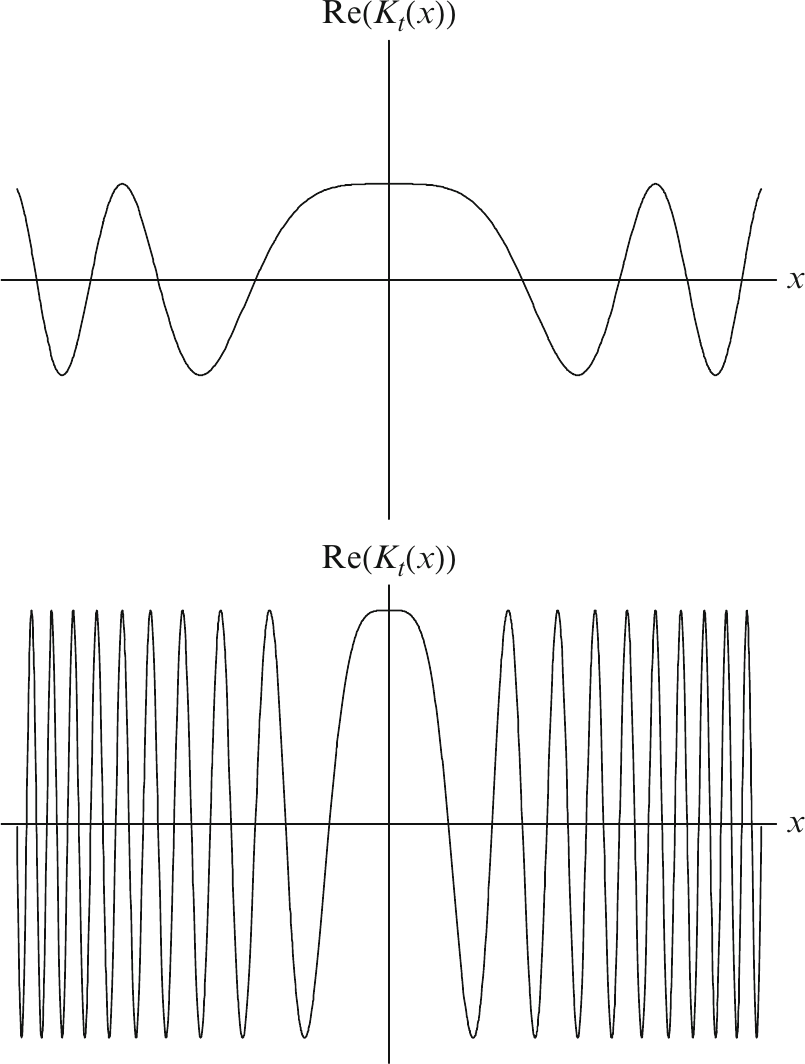
\includegraphics[width=.72\textwidth]{figures/figure-4-1.png}
  \caption{当 \(t=1\)(上图)和 \(t=0.2\)(下图)时,\(K_{t}(x)\) 的实部.}
  \label{fig:free-kernel}
\end{figure}
这里的平方根取实部为正的那个.函数 \(K_{t}\) 称为自由 Schrödinger 方程的基本解(见图~\ref{fig:free-kernel}).直接求导即可验证,\(K_{t}\) 确实满足自由 Schrödinger 方程.

\begin{theorem}[自由方程的卷积公式]\label{thm:free-convolution}
设 \(\psi_{0}\in L^{2}(\mathbb{R})\cap L^{1}(\mathbb{R})\).若 \(\psi(x,t)\) 如式~\eqref{eq:free-fourier-solution} 定义,则对所有 \(t\ne0\),有
\begin{equation}
\psi(x,t)=\sqrt{\frac{m}{2\pi i\hbar t}}
\int_{-\infty}^{\infty}
\exp\left(\frac{im(x-y)^{2}}{2\hbar t}\right)\psi_{0}(y)\,\mathrm{d}y.
\label{eq:free-convolution}
\end{equation}
也就是说,\(\psi(x,t)=(2\pi)^{-1/2}K_{t}*\psi_{0}\),其中 \(K_{t}\) 如式~\eqref{eq:free-kernel}.
\end{theorem}

\begin{proof}
对任意集合 \(E\subset\mathbb{R}\),令 \(\mathbf{1}_{E}\) 表示其示性函数,即在 \(E\) 上为 \(1\),其他地方为 \(0\).对任意正整数 \(n\),\(K_{t}\mathbf{1}_{[-n,n]}\) 属于 \(L^{1}(\mathbb{R})\cap L^{2}(\mathbb{R})\).因此由命题~\ref{app:prop:convolution-fourier},
\[
\mathcal{F}\bigl((K_{t}\mathbf{1}_{[-n,n]})*\psi_{0}\bigr)
=\sqrt{2\pi}\,\mathcal{F}(K_{t}\mathbf{1}_{[-n,n]})\mathcal{F}(\psi_{0}).
\]
由于 \(\psi_{0}\in L^{1}(\mathbb{R})\),容易看出 \(K_{t}\mathbf{1}_{[-n,n]}*\psi_{0}\) 逐点收敛到 \(K_{t}*\psi_{0}\).另一方面,使用练习~\ref{ex:free-gaussian-integral} 中的论证,可以看到 \(\mathcal{F}(K_{t}\mathbf{1}_{[-n,n]})\) 被一个与 \(n\) 无关的常数控制,并逐点收敛到
\[
\frac{1}{\sqrt{2\pi}}\exp\left(-i\frac{\hbar k^{2}}{2m}t\right).
\]
这足以说明式~\eqref{eq:free-convolution-formal} 右端的 Fourier 变换在 \(L^{2}(\mathbb{R})\) 中收敛到
\[
\exp\left(-i\frac{\hbar k^{2}}{2m}t\right)\widehat{\psi}_{0}(k).
\]
由 Plancherel 定理,\(K_{t}\mathbf{1}_{[-n,n]}*\psi_{0}\) 也必须在 \(L^{2}(\mathbb{R})\) 中收敛,而其 \(L^{2}\) 极限必须与逐点极限 \(K_{t}*\psi_{0}\) 一致.对式~\eqref{eq:free-convolution-formal} 两边取极限,就得到所需的 Fourier 变换.

一般来说,要把某个函数称为方程的基本解,还应要求当 \(t\to0\) 时,该函数在分布意义下收敛到 Dirac \(\delta\) 函数(例题~\ref{app:ex:dirac}).由于对每个 \(t\),\(|K_{t}(x)|\) 与 \(x\) 无关,初看之下可能怀疑 \(K_{t}\) 是否有这个性质.另一方面,\(K_{t}(x)\) 除了在 \(x=0\) 附近之外都快速振荡(见图~\ref{fig:free-kernel}).这种振荡使 \(K_{t}(x)\) 与良好函数 \(\psi(x)\) 的积分很小,只有 \(x=0\) 附近的积分部分例外.事实上,由于 \(K_{t}\) 的 Fourier 变换在 \(t\to0\) 时收敛到常函数 \(1/\sqrt{2\pi}\)(这正是形式上取 Dirac \(\delta\) 函数 Fourier 变换所得的结果),不难证明 \(K_{t}\) 确实收敛到 \(\delta\) 函数.细节留给读者.
\end{proof}

\section{波包传播:第一种方法}\label{sec:wave-packet-first}

考虑 \(\mathbb{R}^{1}\) 上的自由 Schrödinger 方程,初始条件 \(\psi_{0}\) 是一个“波包”,即复指数乘以某个将 \(\psi_{0}\) 局部化在空间中的函数.具体取
\begin{equation}
\psi_{0}(x)=e^{ip_{0}x/\hbar}A_{0}(x),
\label{eq:initial-wave-packet}
\end{equation}
其中 \(A_{0}\) 是实的正函数,\(p_{0}\) 是非零实数.(\(p_{0}=0\) 的情形应另行处理.)还假设相对于 \(e^{ip_{0}x/\hbar}\),\(A_{0}\)“变化缓慢”;这意味着在 \(e^{ip_{0}x/\hbar}\) 的许多个周期内,\(A_{0}\) 近似为常数.(稍后会给出“变化缓慢”条件的更精确定义.)因此,如果在只包含几个 \(e^{ip_{0}x/\hbar}\) 周期的小距离尺度上观察 \(\psi_{0}(x)\),它看起来就像常数乘以 \(e^{ip_{0}x/\hbar}\),而后者表示动量为 \(p_{0}\) 的粒子.于是,我们预期 \(\psi_{0}\) 表示一个动量近似等于 \(p_{0}\) 的粒子.

现在尝试用波函数的振幅和相位表示自由 Schrödinger 方程的解.写
\[
\psi(x,t)=A(x,t)e^{i\theta(x,t)},
\]
其中 \(A,\theta\) 是实值函数.把这个表达式代入自由 Schrödinger 方程,并约去每一项中的 \(e^{i\theta(x,t)}\),得到
\begin{equation}
\frac{\partial A}{\partial t}
+iA\frac{\partial\theta}{\partial t}
=\frac{i\hbar}{2m}\frac{\partial^{2}A}{\partial x^{2}}
-\frac{\hbar}{m}\frac{\partial A}{\partial x}\frac{\partial\theta}{\partial x}
-\frac{i\hbar}{2m}A\left(\frac{\partial\theta}{\partial x}\right)^{2}
-\frac{i\hbar}{2m}A\frac{\partial^{2}\theta}{\partial x^{2}}.
\label{eq:amplitude-phase-equation}
\end{equation}
因为 \(A,\theta\) 为实值函数,可以分别令式~\eqref{eq:amplitude-phase-equation} 的实部和虚部相等,得到
\begin{equation}
\frac{\partial A}{\partial t}
=-\frac{\hbar}{m}\frac{\partial A}{\partial x}\frac{\partial\theta}{\partial x}
-\frac{\hbar}{2m}A\frac{\partial^{2}\theta}{\partial x^{2}},
\label{eq:amplitude-equation}
\end{equation}
以及(把虚部除以 \(A\) 后)
\begin{equation}
\frac{\partial\theta}{\partial t}
=\frac{\hbar}{2mA}\frac{\partial^{2}A}{\partial x^{2}}
-\frac{\hbar}{2m}\left(\frac{\partial\theta}{\partial x}\right)^{2}.
\label{eq:phase-equation}
\end{equation}
这个偏微分方程组的任意解都会给出自由 Schrödinger 方程的解 \(\psi(x,t)=A(x,t)e^{i\theta(x,t)}\).

由于我们假设相对于 \(\theta\),\(A\)“变化缓慢”,自然会认为式~\eqref{eq:phase-equation} 右端第一项相对于第二项很小.也就是说,我们把“变化缓慢”理解为
\begin{equation}
\frac{1}{A}\frac{\partial^{2}A}{\partial x^{2}}
\ll\left(\frac{\partial\theta}{\partial x}\right)^{2},
\label{eq:slowly-varying}
\end{equation}
其中 \(\ll\) 表示“远小于”.我们选取在 \(t=0\) 时满足式~\eqref{eq:slowly-varying} 的初始条件,并假定它至少在小的正时间内继续成立.于是(作为一阶近似)可以从式~\eqref{eq:phase-equation} 右端删去第一项,得到简化方程
\begin{equation}
\frac{\partial\theta}{\partial t}
=-\frac{\hbar}{2m}\left(\frac{\partial\theta}{\partial x}\right)^{2}.
\label{eq:approximate-phase}
\end{equation}

现在寻找方程~\eqref{eq:amplitude-equation} 和~\eqref{eq:approximate-phase} 的解,并取与式~\eqref{eq:initial-wave-packet} 对应的初始条件.

\begin{proposition}[波包传播的第一种近似]\label{prop:wave-packet-first}
满足初始条件 \(\theta(x,0)=p_{0}x/\hbar\) 的方程~\eqref{eq:amplitude-equation} 和~\eqref{eq:approximate-phase} 的一个解为
\begin{align}
\theta(x,t)&=\frac{p_{0}}{\hbar}\left(x-\frac{p_{0}}{2m}t\right),\label{eq:wave-packet-phase}\\
A(x,t)&=A_{0}\left(x-\frac{p_{0}}{m}t\right).\label{eq:wave-packet-amplitude}
\end{align}
这给出自由 Schrödinger 方程的近似解
\begin{equation}
\psi(x,t)=A_{0}\left(x-\frac{p_{0}}{m}t\right)
\exp\left[\frac{i}{\hbar}\left(p_{0}x-\frac{p_{0}^{2}}{2m}t\right)\right].
\label{eq:wave-packet-approximation}
\end{equation}
\end{proposition}

从式~\eqref{eq:wave-packet-phase} 和~\eqref{eq:wave-packet-amplitude} 可以看出,如果“变化缓慢”条件~\eqref{eq:slowly-varying} 在时刻 \(0\) 成立,那么在我们的近似解中,它会对所有正时间继续成立.

\begin{proof}
虽然式~\eqref{eq:approximate-phase} 是非线性方程,但对初始条件 \(\theta(x,0)=p_{0}x/\hbar\),可以找到简单的解
\[
\theta(x,t)=\frac{p_{0}x}{\hbar}-\frac{p_{0}^{2}}{2m\hbar}t
=\frac{p_{0}}{\hbar}\left(x-\frac{p_{0}}{2m}t\right).
\]
由于 \(\partial\theta/\partial x=p_{0}/\hbar\),且 \(\partial^{2}\theta/\partial x^{2}=0\),将其代回式~\eqref{eq:amplitude-equation},得到
\[
\frac{\partial A}{\partial t}
=-\frac{p_{0}}{m}\frac{\partial A}{\partial x}.
\]
这个线性方程以 \(A(x,0)=A_{0}(x)\) 为初始条件的(推测唯一)解为
\[
A(x,t)=A_{0}\left(x-\frac{p_{0}}{m}t\right),
\]
命题得证.
\end{proof}

我们希望,在 \(A_{0}\) 相对于初始相位 \(\theta_{0}(x)=p_{0}x/\hbar\) 变化缓慢的前提下,式~\eqref{eq:wave-packet-approximation} 是原方程~\eqref{eq:amplitude-equation} 和~\eqref{eq:phase-equation} 解的良好近似.不过,直接估计式~\eqref{eq:amplitude-equation}--\eqref{eq:phase-equation} 的解彼此偏离的速度并不容易.因此,我们把近似误差的估计留到下一节;在那里将用不同方法得到同一个近似解.

注意,形如 \(f(x,t)=\phi(x-vt)\) 的函数以恒定速度 \(v\) 向右运动(如果 \(v<0\),当然表示向左运动).振幅 \(A(x,t)\) 和相位因子 \(e^{i\theta(x,t)}\) 都具有这种形式,但对应两个不同的速度.

\begin{conclusion}[群速度与相速度]\label{con:group-phase-velocity}
在自由 Schrödinger 方程的近似解~\eqref{eq:wave-packet-approximation} 中,振幅 \(A(x,t)\) 以速度 \(p_{0}/m\) 运动,而相位 \(\theta(x,t)\) 以速度 \(p_{0}/(2m)\) 运动.这两个速度分别称为群速度和相速度:
\[
\text{相速度}=\frac{p_{0}}{2m},
\qquad
\text{群速度}=\frac{p_{0}}{m}.
\]
\end{conclusion}

相速度公式与前面第~\ref{sec:free-fourier} 节给出的公式一致;那里相速度是自由 Schrödinger 方程纯指数解的传播速度.事实上,取 \(A_{0}\equiv1\),式~\eqref{eq:slowly-varying} 左端恒等于零,于是方程~\eqref{eq:amplitude-equation} 和~\eqref{eq:phase-equation} 的解也确实是原方程的解.

哪个速度是粒子的“真实”速度？答案是群速度.毕竟,粒子位置的概率分布由波函数的振幅决定,而不受相位影响.振幅决定了粒子在哪里(在可确定的程度内).因此,粒子的真实速度应是振幅传播的速度.图~\ref{fig:free-wave-packet} 展示了波包实部的传播,并用阴影区域标出一个峰的运动.相速度决定 \(\psi\) 实部中各个峰的运动速度,而群速度决定整个波包的运动速度.由于我们跟踪的峰明显落后于整个波包的运动,可以看出相速度小于群速度.

\begin{figure}[htbp]
  \centering
  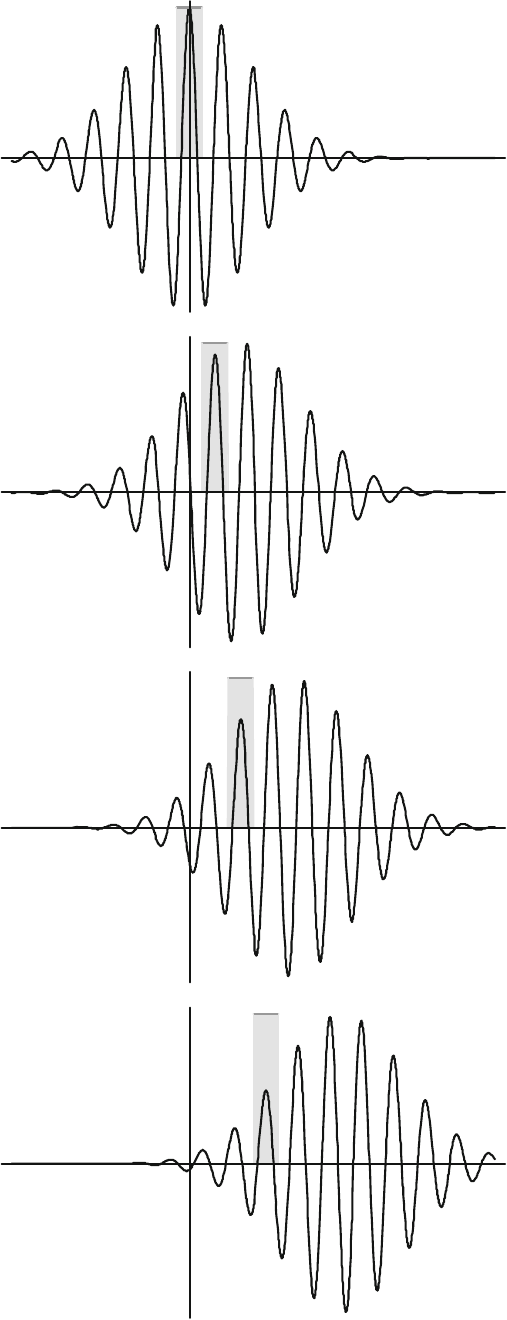
\includegraphics[width=.48\textwidth]{figures/figure-4-2.png}
  \caption{\(\operatorname{Re}[\psi]\) 的传播,其中阴影部分标出了单个峰的运动.}
  \label{fig:free-wave-packet}
\end{figure}

我们应当预期,方程~\eqref{eq:amplitude-equation} 和~\eqref{eq:approximate-phase} 的解会随时间缓慢偏离自由 Schrödinger 方程~\eqref{eq:amplitude-equation} 和~\eqref{eq:phase-equation} 的解.经过足够长时间,近似解与真实解之间可能有明显差异.这一预期将在第~\ref{sec:wave-packet-spread} 节得到确认;那里将研究波包扩散,而这一现象在当前近似中看不到.

\section{波包传播:第二种方法}\label{sec:wave-packet-second}

我们已经看到,自由 Schrödinger 方程的一般解可以通过 Fourier 变换写成
\begin{equation}
\psi(x,t)=\frac{1}{\sqrt{2\pi}}\int_{-\infty}^{\infty}
\widehat{\psi}_{0}(k)\exp[i(kx-\omega(k)t)]\,\mathrm{d}k,
\label{eq:free-fourier-general}
\end{equation}
其中
\[
\omega(k)=\frac{\hbar k^{2}}{2m}.
\]
假设 \(\psi_{0}\) 的近似动量为 \(p_{0}\).于是预期 \(\widehat{\psi}_{0}(k)\) 集中在 \(k_{0}:=p_{0}/\hbar\) 附近.如果确实如此,那么只有接近 \(k_{0}\) 的 \(k\) 值重要.对接近 \(k_{0}\) 的 \(k\),使用一阶 Taylor 展开
\begin{equation}
\omega(k)\approx\omega(k_{0})+\omega'(k_{0})(k-k_{0}).
\label{eq:dispersion-linearization}
\end{equation}

把式~\eqref{eq:dispersion-linearization} 代入式~\eqref{eq:free-fourier-general},两个与 \(k\) 无关的因子可以移到积分号外,得到
\begin{align}
\psi(x,t)
&\approx\frac{1}{\sqrt{2\pi}}e^{i\omega'(k_{0})k_{0}t}e^{-i\omega(k_{0})t}
\int_{-\infty}^{\infty}\widehat{\psi}_{0}(k)
\exp[i k(x-\omega'(k_{0})t)]\,\mathrm{d}k\notag\\
&=e^{i\omega'(k_{0})k_{0}t}e^{-i\omega(k_{0})t}
\psi_{0}(x-\omega'(k_{0})t).
\label{eq:wave-packet-fourier-approx}
\end{align}
注意,\(\psi_{0}(x-\omega'(k_{0})t)\) 前的因子只是与 \(x\) 无关的常数.这些常数不影响系统的“状态”,因为我们已经约定,量子 Hilbert 空间中相差一个常数的两个向量代表同一物理状态.忽略这些常数,剩下的因子 \(\psi_{0}(x-\omega'(k_{0})t)\) 正是以速度 \(\omega'(k_{0})\) 向右平移的函数.因此,波包运动的(近似)速度为
       \[
\text{速度}\approx\omega'(k_{0})
=\frac{\hbar k_{0}}{m}
=\frac{p_{0}}{m}.
\]

考虑 \(\psi_{0}(x)=e^{ik_{0}x}A_{0}(x)\) 的特殊情形,其中 \(A_{0}\) 实且为正.那么式~\eqref{eq:wave-packet-fourier-approx} 变为
\[
e^{i\omega'(k_{0})k_{0}t}e^{-i\omega(k_{0})t}
e^{ik_{0}(x-\omega'(k_{0})t)}
A_{0}(x-\omega'(k_{0})t).
\]
约去指数中包含 \(\omega'(k_{0})k_{0}t\) 的项,得到
\[
\psi(x,t)\approx e^{i(k_{0}x-\omega(k_{0})t)}
A_{0}(x-\omega'(k_{0})t).
\]
回忆 \(p_{0}=\hbar k_{0}\),代入 \(\omega\) 的公式可知,这个 \(\psi(x,t)\) 的近似正是我们在命题~\ref{prop:wave-packet-first} 中通过另一种方法得到的近似.

与第~\ref{sec:wave-packet-first} 节一样,自由 Schrödinger 方程的纯指数解传播速度 \(\omega(k_{0})/k_{0}=\hbar k_{0}/(2m)\) 与整个波包的传播速度不同.由式~\eqref{eq:wave-packet-fourier-approx} 可见,波包以 \(\omega'(k_{0})=\hbar k_{0}/m\) 的速度传播.总结如下.

\begin{proposition}[群速度与相速度的 Fourier 观点]\label{prop:group-phase-velocity}
自由 Schrödinger 方程的纯指数解传播的速度为
\[
\text{相速度}=\frac{\omega(k_{0})}{k_{0}}
=\frac{\hbar k_{0}}{2m}
=\frac{p_{0}}{2m}.
\]
相比之下,波包传播的(近似)速度为
\[
\text{群速度}
=\left.\frac{\mathrm{d}\omega}{\mathrm{d}k}\right|_{k=k_{0}}
=\frac{\hbar k_{0}}{m}
=\frac{p_{0}}{m}.
\]
\end{proposition}

第~\ref{sec:wave-packet-first} 节的方法不容易直接给出近似误差的大小估计.不过,在本节中可以通过比较精确解与近似解的 Fourier 变换来估计误差.为此定义
\begin{equation}
\kappa:=\left(\int_{-\infty}^{\infty}
|\widehat{\psi}_{0}(k)|^{2}(k-k_{0})^{4}\,\mathrm{d}k\right)^{1/4}.
\label{eq:wave-packet-concentration}
\end{equation}
\(\kappa\) 大致是 \(\widehat{\psi}_{0}(k)\) 大部分集中所在的、以 \(k_{0}\) 为中心的区间宽度的一半.例如,如果 \(\widehat{\psi}_{0}\) 支集包含在 \([k_{0}-\varepsilon,k_{0}+\varepsilon]\) 中,并且 \(\psi_{0}\)(因而 \(\widehat{\psi}_{0}\))是单位向量,则 \(\kappa\le\varepsilon\).更常见的集中度量会用 \((k-k_{0})^{2}\) 替换四次幂,并用平方根而非四次根.不过,式~\eqref{eq:wave-packet-concentration} 中的“四次”度量正是本节误差估计中出现的量.

\begin{proposition}[波包近似的误差估计]\label{prop:wave-packet-error}
设 \(\psi(x,t)\) 是初始条件为 \(\psi_{0}\) 的自由 Schrödinger 方程精确解,\(\phi(x,t)\) 是式~\eqref{eq:wave-packet-fourier-approx} 右端给出的近似解,则有 \(L^{2}\) 估计
\begin{equation}
\|\psi(x,t)-\phi(x,t)\|_{L^{2}(\mathbb{R})}
\le\frac{|t|\hbar\kappa^{2}}{2m}
=|t|\,\omega(\kappa),
\label{eq:wave-packet-error}
\end{equation}
其中 \(L^{2}\) 范数固定 \(t\) 关于 \(x\) 取,\(\omega\) 由式~\eqref{eq:free-dispersion} 定义.
\end{proposition}

式~\eqref{eq:wave-packet-error} 意味着,只要
\[
|t|\ll\frac{1}{\omega(\kappa)},
\]
\(L^{2}\) 意义下的误差就会很小.如果 \(\kappa\ll k_{0}\),那么 \(1/\omega(\kappa)\) 会远大于 \(1/\omega(k_{0})\).这意味着真实解和近似解开始明显偏离的时间尺度,远长于近似解振荡的时间尺度.

\begin{proof}
记 \(\widehat{\psi}(k,t)\) 和 \(\widehat{\phi}(k,t)\) 为固定 \(t\) 关于 \(x\) 的 Fourier 变换.由式~\eqref{eq:free-fourier-general} 可读出
\[
\widehat{\psi}(k,t)=e^{-i\omega(k)t}\widehat{\psi}_{0}(k).
\]
另一方面,\(\widehat{\phi}(k,t)\) 由 \(\widehat{\psi}(k,t)\) 将 \(\omega(k)\) 替换为式~\eqref{eq:dispersion-linearization} 右端得到.直接计算可得
\[
\omega(k)-\bigl(\omega(k_{0})+\omega'(k_{0})(k-k_{0})\bigr)
=\frac{\hbar}{2m}(k-k_{0})^{2}.
\]
利用初等估计 \(|e^{i\theta}-e^{i\varphi}|\le|\theta-\varphi|\),得到
\[
|\widehat{\psi}(k,t)-\widehat{\phi}(k,t)|
\le\frac{|t|\hbar}{2m}(k-k_{0})^{2}|\widehat{\psi}_{0}(k)|.
\]
于是由 Plancherel 定理和 \(\kappa\) 的定义得到式~\eqref{eq:wave-packet-error}.
\end{proof}

\section{波包的扩散}\label{sec:wave-packet-spread}

我们用粒子位置的不确定度 \(\Delta_{\psi}X\)(定义~\ref{def:quantum-uncertainty})作为 \(\psi(x)\) 这个函数“宽度”的度量.在前两节所考虑的近似层次上,自由粒子的位置不确定度与时间无关.毕竟,在近似解~\eqref{eq:wave-packet-approximation} 中,波函数的振幅只以群速度向右平移,而形状不变.不过,更精确的计算表明,经过足够长时间后,波包会在空间中扩散.(练习~\ref{ex:free-spread-rate} 可以帮助理解扩散发生的时间尺度.)

利用第~3 章的命题~\ref{prop:expectation-evolution},无需求出完整的 Schrödinger 方程解,就可以计算粒子位置不确定度的时间演化.对自由粒子,Hamilton 算子就是 \(P^{2}/(2m)\),它与 \(P\) 对易.因此,粒子的动量期望值、不确定度(事实上包括动量的整个概率分布)都与时间无关.另一方面,要计算 \(\langle X\rangle\) 和 \(\langle X^{2}\rangle\) 的时间依赖,可以使用命题~\ref{prop:expectation-evolution} 以及对易关系 \([X,P]=i\hbar I\)(命题~\ref{prop:canonical-commutation-one}).

\begin{proposition}[自由粒子的波包扩散]\label{prop:free-wave-spread}
若波函数 \(\psi(x,t)\) 按照 \(\mathbb{R}^{1}\) 上的自由 Schrödinger 方程演化,则
\begin{align}
\langle X\rangle_{\psi(t)}
&=\langle X\rangle_{\psi_{0}}+\frac{t}{m}\langle P\rangle_{\psi_{0}},\label{eq:free-position-time}\\
\langle X^{2}\rangle_{\psi(t)}
&=\langle X^{2}\rangle_{\psi_{0}}
+\frac{t}{m}\langle XP+PX\rangle_{\psi_{0}}
+\frac{t^{2}}{m^{2}}\langle P^{2}\rangle_{\psi_{0}}.\label{eq:free-position-square-time}
\end{align}
从而
\begin{equation}
(\Delta_{\psi(t)}X)^{2}
=(\Delta_{\psi_{0}}X)^{2}
+\frac{t}{m}\left(\langle XP+PX\rangle_{\psi_{0}}
-2\langle X\rangle_{\psi_{0}}\langle P\rangle_{\psi_{0}}\right)
+\frac{t^{2}}{m^{2}}(\Delta_{\psi_{0}}P)^{2}.
\label{eq:free-position-uncertainty}
\end{equation}
\end{proposition}

对于 \(L^{2}(\mathbb{R})\) 中的单位向量 \(\psi_{0}\),动量不确定度 \(\Delta_{\psi_{0}}P\) 不可能为零,因为不确定度为零意味着 \(\psi_{0}\) 是动量算子的特征向量,而 \(P\) 的特征向量是形如 \(e^{ikx}\) 的函数,它们不属于 \(L^{2}(\mathbb{R})\).因此,式~\eqref{eq:free-position-uncertainty} 中 \(t^{2}\) 项的系数永不为零,从而当 \(t\to\infty\) 时,\(\Delta_{\psi(t)}X\to\infty\).

\begin{proof}
计算得
\[
[P^{2},X]=P[P,X]+[P,X]P=-2i\hbar P.
\]
因此(正如我们在第~\ref{subsec:expected-position-momentum} 节已经指出的),
\[
\frac{\mathrm{d}}{\mathrm{d}t}\langle X\rangle_{\psi(t)}
=\left\langle\frac{i}{\hbar}(-2i\hbar P)\right\rangle_{\psi(t)}
=\frac{\langle P\rangle_{\psi(t)}}{m}
=\frac{\langle P\rangle_{\psi_{0}}}{m},
\]
其中最后一个等号使用了动量期望值与时间无关这一事实.由于 \(\langle X\rangle_{\psi(t)}\) 的导数是常数,它关于 \(t\) 是线性的,于是得到命题中的第一个结果.

另一方面,直接计算可得
\[
[P^{2},X^{2}]
=-2i\hbar(PX+XP),
\]
以及
\[
[P^{2},PX+XP]=-4i\hbar P^{2}.
\]
因此
\[
\frac{\mathrm{d}}{\mathrm{d}t}\langle X^{2}\rangle_{\psi(t)}
=\frac{1}{m}\langle XP+PX\rangle_{\psi(t)},
\]
并且
\[
\frac{\mathrm{d}^{2}}{\mathrm{d}t^{2}}\langle X^{2}\rangle_{\psi(t)}
=\frac{2}{m^{2}}\langle P^{2}\rangle_{\psi(t)}
=\frac{2}{m^{2}}\langle P^{2}\rangle_{\psi_{0}}.
\]
由于 \(\langle X^{2}\rangle_{\psi(t)}\) 的二阶导数与时间无关,它关于 \(t\) 是二次多项式;其系数由 \(t=0\) 时 \(\langle X\rangle_{\psi(t)}\) 的值以及前两个时间导数确定.这给出式~\eqref{eq:free-position-square-time}.最后一个结果直接计算即可得到.
\end{proof}

\section{练习}\label{sec:chapter4-exercises}

\begin{exercise}\label{ex:free-weak-solution}
局部可积函数 \(\psi(x,t)\) 在弱(或分布)意义下满足自由 Schrödinger 方程,是指对每个光滑紧支集函数 \(\chi\),都有
\begin{equation}
\int_{\mathbb{R}^{2}}\psi(x,t)\left(\frac{\partial\chi}{\partial t}
+\frac{i\hbar}{2m}\frac{\partial^{2}\chi}{\partial x^{2}}\right)\,\mathrm{d}x\,\mathrm{d}t=0.
\label{eq:free-weak-equation}
\end{equation}
(式~\eqref{eq:free-weak-equation} 的得到方式是,假定 \(\partial\psi/\partial t-(i\hbar/2m)\partial^{2}\psi/\partial x^{2}=0\),再与 \(\chi(x,t)\) 相乘并形式地分部积分.)
\begin{enumerate}
\item 证明,如果 \(\psi(x,t)\) 关于 \(x,t\) 光滑,则它在逐点意义下满足自由 Schrödinger 方程,当且仅当它在弱意义下满足自由 Schrödinger 方程.提示:命题~\ref{app:prop:distribution-constant} 可能有用.
\item 对任意 \(\psi_{0}\in L^{2}(\mathbb{R})\),按定义~\ref{def:free-l2-evolution} 定义 \(\psi(x,t)\).证明 \(\psi\) 在弱意义下满足自由 Schrödinger 方程.先证明对每个 \(A\),函数
\[
\psi_{A}(x,t)=\frac{1}{\sqrt{2\pi}}\int_{-A}^{A}
\widehat{\psi}_{0}(k)e^{i(kx-\omega(k)t)}\,\mathrm{d}k
\]
在弱意义下满足自由 Schrödinger 方程.
\end{enumerate}
\end{exercise}

\begin{exercise}\label{ex:free-gaussian-integral}
\begin{enumerate}
\item 证明,对任意 \(\operatorname{Re}(a)>0\) 的复数 \(a\),有
\[
\int_{-\infty}^{\infty}e^{-x^{2}/(2a)}\,\mathrm{d}x
=\iint_{\mathbb{R}^{2}}e^{-(x^{2}+y^{2})/(2a)}\,\mathrm{d}x\,\mathrm{d}y
=2\pi a,
\]
其中 \(\mathbb{R}^{2}\) 上的积分可用极坐标计算.推出(平方根取实部为正)
\[
\int_{-\infty}^{\infty}e^{-x^{2}/(2a)}\,\mathrm{d}x=\sqrt{2\pi a}.
\]
\item 证明,对任意 \(A,B>0\) 以及任意非零复数 \(a\),有
\[
\int_{A}^{B}e^{-x^{2}/(2a)}\,\mathrm{d}x
=\left.-\frac{a}{x}e^{-x^{2}/(2a)}\right|_{A}^{B}
-a\int_{A}^{B}\frac{1}{x^{2}}e^{-x^{2}/(2a)}\,\mathrm{d}x.
\]
利用它证明,当非零 \(a\) 满足 \(\operatorname{Re}(a)\ge0\) 时,只要把积分理解为广义积分(即取 \([-A,A]\) 上积分并令 \(A\to\infty\) 的极限),式~\eqref{eq:free-kernel} 中的积分收敛.
\item 证明 (a) 的结论对非零且 \(\operatorname{Re}(a)=0\) 的 \(a\) 也成立.提示:给定 \(\beta\ne0\),证明当 \(A\) 很大时,从 \(A\) 到 \(\infty\) 的 \(\exp[-x^{2}/(2(\alpha+i\beta))]\) 积分,对 \(\alpha\in[0,1]\) 一致地很小.
\item 证明(积分理解为广义积分,平方根取实部为正)
\[
\frac{1}{2\pi}\int_{-\infty}^{\infty}e^{ikx}e^{-it\hbar k^{2}/(2m)}\,\mathrm{d}k
=\sqrt{\frac{m}{2\pi i\hbar t}}e^{imx^{2}/(2t\hbar)}.
\]
\end{enumerate}
\end{exercise}

\begin{exercise}\label{ex:convolution-smooth}
设 \(\phi\) 是 Schwartz 函数(定义~\ref{app:def:schwartz}),\(\psi\in L^{2}(\mathbb{R})\).证明卷积 \(\phi*\psi\) 是光滑函数(无穷可微).
\end{exercise}

\begin{exercise}\label{ex:heat-equation}
考虑函数 \(\psi(x,t)\) 的热方程
\[
\frac{\partial\psi}{\partial t}
=\alpha\frac{\partial^{2}\psi}{\partial x^{2}},
\]
其中 \(\alpha\) 是常数,初始条件为 \(\psi(x,0)=\psi_{0}(x)\).
\begin{enumerate}
\item 假设对每个 \(t\),\(\psi(x,t)\) 关于 \(x\) 足够良好.推导热方程解关于 \(x\) 的 Fourier 变换 \(\widehat{\psi}(k,t)\) 所满足的微分方程,并求出满足 \(\widehat{\psi}(k,0)=\widehat{\psi}_{0}(k)\) 的解.
\item 把热方程的解表示为 \(\psi_{0}\) 与热方程某个“基本解”的卷积.
\end{enumerate}
\begin{note}
正如第~20 章将讨论的,热方程可以看成自由 Schrödinger 方程的某种“虚时间”版本.
\end{note}
\end{exercise}

\begin{exercise}\label{ex:gaussian-wave-packet}
设自由 Schrödinger 方程的初始相位为 \(\theta_{0}(x)=p_{0}x/\hbar\),初始振幅为 \(A_{0}(x)\),如式~\eqref{eq:initial-wave-packet}.再假设
\[
A_{0}(x)=\exp\left(-\frac{1}{2}\left(\frac{x-x_{0}}{L}\right)^{2}\right).
\]
注意,\(A_{0}\) 以 \(x_{0}\) 为中心,参数 \(L\) 衡量初始波包在空间中的宽度.具有这种 \(A_{0}\) 的 \(\psi_{0}(x)=e^{ip_{0}x/\hbar}A_{0}(x)\) 称为 Gaussian 波包.计算
\[
\left(\frac{\partial\theta_{0}}{\partial x}\right)^{-2}
\left(\frac{1}{A_{0}}\frac{\partial^{2}A_{0}}{\partial x^{2}}\right).
\]
假设 \(\hbar\) 相对于 \(Lp_{0}\) 很小,证明除非在初始波包非常小的点处,否则上式很小.
\begin{note}
这说明对 Gaussian 波包而言,“变化缓慢”假设~\eqref{eq:slowly-varying} 是合理的.
\end{note}
\end{exercise}

\begin{exercise}\label{ex:klein-gordon}
Klein--Gordon 方程是 Schrödinger 方程的一种拟议的相对论替代理论:
\[
\frac{1}{c^{2}}\frac{\partial^{2}\psi}{\partial t^{2}}
=\frac{\partial^{2}\psi}{\partial x^{2}}-\frac{m^{2}c^{2}}{\hbar^{2}}\psi,
\]
其中 \(m>0\) 是粒子质量,\(c\) 是光速.
\begin{enumerate}
\item 求 Klein--Gordon 方程的色散关系,即找出使 \(\exp[i(kx-\omega(k)t)]\) 成为方程解的 \(\omega(k)\).
\item 证明相速度 \(\omega(k)/k\) 满足 \(|\omega(k)/k|>c\),群速度 \(\mathrm{d}\omega(k)/\mathrm{d}k\) 满足 \(|\mathrm{d}\omega/\mathrm{d}k|<c\),并且
\[
(\text{相速度})(\text{群速度})=c^{2}.
\]
\end{enumerate}
\begin{note}
由于 Klein--Gordon 方程关于时间是二阶的,对每个 \(k\) 有两个可能的 \(\omega(k)\),一个为正,一个为负.(b) 的结论对 \(\omega(k)\) 的两支都成立.
\end{note}
\end{exercise}

\begin{exercise}\label{ex:free-spread-rate}
考虑按自由 Schrödinger 方程演化的波函数 \(\psi(t)\) 的位置不确定度 \(\Delta_{\psi(t)}X\).证明对所有 \(t\),
\begin{equation}
\left|\frac{\mathrm{d}}{\mathrm{d}t}\Delta_{\psi(t)}X\right|
\le\frac{\Delta_{\psi_{0}}P}{m},
\label{eq:free-spread-bound}
\end{equation}
并证明
\[
\lim_{t\to+\infty}\frac{\mathrm{d}}{\mathrm{d}t}\Delta_{\psi(t)}X
=\frac{\Delta_{\psi_{0}}P}{m}.
\]
\begin{note}
相比之下,
\[
\frac{\mathrm{d}}{\mathrm{d}t}\langle X\rangle_{\psi(t)}
=\frac{\langle P\rangle_{\psi_{0}}}{m}.
\]
如果 \(\widehat{\psi}_{0}(k)\) 集中在非零数 \(k_{0}=p_{0}/\hbar\) 附近的一个足够小的区域,那么 \(\Delta_{\psi_{0}}P\) 会远小于 \(\langle P\rangle_{\psi_{0}}\).比较式~\eqref{eq:free-spread-bound} 与上述式子可知,此时波包扩散的速率相对于波包运动的速率很小.
\end{note}
\end{exercise}

\chapter{方势阱中的粒子}\label{chap:square-well}

\section{定态 Schrödinger 方程}\label{sec:square-well-time-independent}

先考察经典粒子在方势阱中的行为.若粒子能量为负,则粒子必须位于势阱中;它以恒定速度运动,直到撞到势阱边缘,随后瞬间从墙壁反射,并以相同速率向相反方向运动.若粒子能量为正,则它始终沿同一方向运动;在势阱外和势阱内,速度分别为不同的常数.

在量子情形中,我们主要关注 Schrödinger 算子的负特征值(\(E<0\))所对应的特征向量.当然,在量子理论中,能量特征向量除一个整体相位因子外不随时间变化.不过,由于能量为负的经典粒子在势阱各部分停留的时间相同,可以预期量子粒子在势阱各部分被发现的概率近似相等.对于“高激发态”,例如图~\ref{fig:square-well-deep-excited} 所示的状态,这一预期确实会实现.但量子粒子在势阱外被发现的概率虽小却非零,而经典粒子不可能出现在那里.

我们的目标是研究定态 Schrödinger 方程,即特征值方程
\begin{equation}
-\frac{\hbar^{2}}{2m}\frac{\mathrm{d}^{2}\psi}{\mathrm{d}x^{2}}
+V(x)\psi(x)=E\psi(x),
\label{eq:square-well-schrodinger}
\end{equation}
其中特征值 \(E\) 和相应特征向量 \(\psi\)(物理学术语称“特征函数”)都尚未确定.作为二阶线性常微分方程,式~\eqref{eq:square-well-schrodinger} 对任意 \(E\) 总有一个二维解空间.不过,我们要找的是属于量子 Hilbert 空间 \(L^{2}(\mathbb{R})\) 的解.实际上只有有限多个 \(E\)(全都满足 \(E<0\))使得式~\eqref{eq:square-well-schrodinger} 在 \(L^{2}(\mathbb{R})\) 中存在非零解.因此,Schrödinger 算子 \(\widehat H\) 在零以下具有离散谱,在零以上具有连续谱.

本节考虑一个简单但有启发性的例子,它可以用初等方法求解.我们在 \(\mathbb{R}^{1}\) 中取势能
\begin{equation}
V(x)=
\begin{cases}
-C,&-A\le x\le A,\\
0,&|x|>A,
\end{cases}
\label{eq:square-well-potential}
\end{equation}
\begin{figure}[htbp]
  \centering
  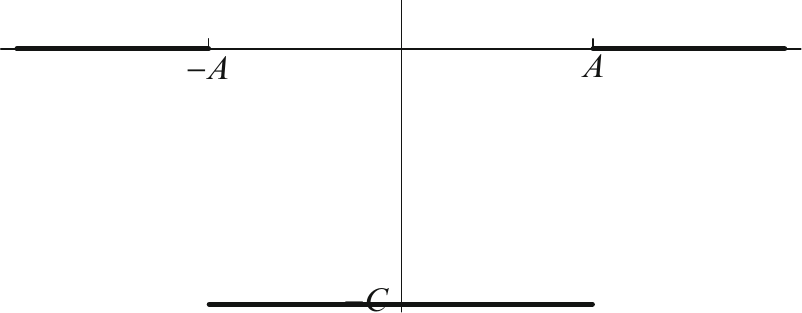
\includegraphics[width=.72\textwidth]{figures/figure-5-1.png}
  \caption{方势阱的势能.}
  \label{fig:square-well-potential}
\end{figure}
其中 \(A,C\) 是正数.区域 \(-A\le x\le A\) 称为势能的“方势阱”(图~\ref{fig:square-well-potential}).

\section{定义域问题与匹配条件}\label{sec:square-well-domain}

在开始求解式~\eqref{eq:square-well-schrodinger} 之前,必须注意 Hamilton 算子的无界性.左端的 Schrödinger 算子
\[
\widehat H=-\frac{\hbar^{2}}{2m}\frac{\mathrm{d}^{2}}{\mathrm{d}x^{2}}+V(X)
\]
是无界算子,即不存在常数 \(C\),使得对所有 \(\psi\) 都有 \(\|\widehat H\psi\|\le C\|\psi\|\),其中范数是 \(L^{2}\) 范数.另一方面,我们希望以某种方式定义 \(\widehat H\),使其为自伴算子.但根据关于无界算子的基本结论,一个定义在整个 Hilbert 空间上的自伴算子必须有界.

因此,\(\widehat H\) 不会定义在整个 Hilbert 空间 \(L^{2}(\mathbb{R})\) 上,而只定义在其中的一个稠密子空间上.实际而言,说 \(\widehat H\) 没有定义在整个 Hilbert 空间上,只是说对于 \(L^{2}(\mathbb{R})\) 中许多函数 \(\psi\),二阶导数 \(\mathrm{d}^{2}\psi/\mathrm{d}x^{2}\) 不存在,或者虽然存在却不属于 \(L^{2}(\mathbb{R})\).在本例中势能 \(V\) 有界,所以只要 \(\psi\in L^{2}(\mathbb{R})\),\(V\psi\) 总属于 \(L^{2}(\mathbb{R})\).

由于方势阱的势能有界,Hamilton 算子 \(\widehat H=P^{2}/(2m)+V(X)\) 的定义域与动能算子 \(P^{2}/(2m)=-(\hbar^{2}/2m)\mathrm{d}^{2}/\mathrm{d}x^{2}\) 的定义域相同.第~9 章将看到,动能算子的定义域可以描述为:那些属于 \(L^{2}(\mathbb{R})\) 且其弱导数(或分布导数,见附录~\ref{app:def:distribution-derivative})\(\mathrm{d}^{2}\psi/\mathrm{d}x^{2}\) 仍属于 \(L^{2}(\mathbb{R})\) 的函数空间.这个条件等价于:存在某个 \(L^{2}\) 函数 \(\phi\),使得 \(\psi\) 是 \(\phi\) 的二重积分(对积分常数作某种选择).

另一方面,由于方势阱的势能是分段常数,式~\eqref{eq:square-well-schrodinger} 的任意解在 \(x=\pm A\) 之外都光滑,并且 \(\psi\) 与 \(\psi'\) 在 \(A\) 和 \(-A\) 处都有左右极限.事实上,在区间 \((-\infty,-A)\)、\((-A,A)\) 和 \((A,\infty)\) 上,解都只是(实或复)指数函数的线性组合.对这种函数,不难判断何时属于 \(\widehat H\) 的定义域.

\begin{proposition}[方势阱的定义域条件]\label{prop:square-well-domain}
设 \(\psi\) 在区间 \((-\infty,-A)\)、\((-A,A)\) 和 \((A,\infty)\) 上分别光滑.那么,\(\psi\) 属于势能函数由式~\eqref{eq:square-well-potential} 给出的 \(\widehat H\) 的定义域,当且仅当:
\begin{enumerate}
\item \(\psi\) 与 \(\mathrm{d}\psi/\mathrm{d}x\) 在 \(x=\pm A\) 处连续;
\item \(\mathrm{d}^{2}\psi/\mathrm{d}x^{2}\) 属于 \(L^{2}(\mathbb{R})\).
\end{enumerate}
\end{proposition}

\begin{proof}
先假设 \(\psi\) 满足 (1) 和 (2).不难看出,\(\psi\) 的分布二阶导数就是在 \(x\ne\pm A\) 处按通常逐点意义计算的 \(\mathrm{d}^{2}\psi/\mathrm{d}x^{2}\)(在 \(x=\pm A\) 这两个测度为零的点,可以不定义二阶导数).因此,以分布意义计算的二阶导数属于 \(L^{2}(\mathbb{R})\).

反过来,如果 \(\psi\) 或 \(\psi'\) 在 \(x=A\) 或 \(x=-A\) 处有间断,那么分布导数将包含这些点处 \(\delta\) 函数的非零倍数,或者 \(\delta\) 函数导数的非零倍数.但 \(\delta\) 函数及其导数都不是平方可积函数.因此必须满足连续性条件.
\end{proof}

来理解 \(\psi\) 和 \(\mathrm{d}\psi/\mathrm{d}x\) 的连续性条件在实际中的含义.由于 \(V\) 在 \((-\infty,-A)\) 上为常数,可以很容易地在该区间求解式~\eqref{eq:square-well-schrodinger};解空间是二维的.一旦从这个解空间中选定一个解,那么当 \(x\) 从左侧趋于 \(-A\) 时,\(\psi\) 和 \(\mathrm{d}\psi/\mathrm{d}x\) 的值就成为在 \((-A,A)\) 上求解方程的初始条件.因此,\(\psi\) 与 \(\psi'\) 的连续性为 \((-\infty,-A)\) 上的解与 \((-A,A)\) 上的解提供了“匹配条件”.不能在 \((-\infty,-A)\) 和 \((-A,A)\) 上任意分别选择解;在边界处,\(\psi\) 和 \(\psi'\) 的值必须匹配.(在具有不连续系数的初等常微分方程中,也会出现同样的匹配条件.)

一旦在 \((-\infty,-A)\) 上选定一个解,就能唯一地把它延拓到 \((-A,A)\);随后在 \(A\) 左侧趋近时 \(\psi,\psi'\) 的值又成为在 \((A,\infty)\) 上求解方程的初始条件.结论是:一旦在 \((-\infty,-A)\) 的二维解空间中选择一个解,就没有额外选择;微分方程与匹配条件给出了把解从 \((-\infty,-A)\) 唯一延拓到整个实轴的方式.

\section{寻找平方可积解}\label{sec:square-well-solutions}

如果 \(E>0\),那么在 \(x<-A\) 的任意解都是两个复指数的线性组合;这样的函数除非恒等于零,否则不可能平方可积.如果我们在 \(x<-A\) 区域令 \(\psi\) 恒等于零,那么连续性条件要求 \(x\to-A^{+}\) 时 \(\psi\) 和 \(\psi'\) 都趋于零.因此 \(-A\) 处的匹配条件迫使 \([-A,A]\) 上的解也恒等于零;最后通过 \(x=A\) 的匹配,得到 \([A,\infty)\) 上的零解.所以,当 \(E>0\) 时,满足命题~\ref{prop:square-well-domain} 连续性条件的任何解都恒等于零.\(E=0\) 时分析相同,此时在 \((-\infty,A]\) 上的解形如 \(c_{1}+c_{2}x\),只有 \(c_{1}=c_{2}=0\) 时才平方可积.

因此,要想得到既平方可积又属于 \(\widehat H\) 定义域的解,必须取 \(E<0\).当 \(E<0\) 时,\((-\infty,-A)\) 上的解是 \(\exp(\alpha x)\) 和 \(\exp(-\alpha x)\) 的线性组合,其中
\begin{equation}
\alpha=\frac{\sqrt{2m|E|}}{\hbar}.
\label{eq:square-well-alpha}
\end{equation}
为了使 \(\psi\) 在 \((-\infty,-A)\) 上平方可积,\(\exp(-\alpha x)\) 的系数必须为零,因为当 \(x\to-\infty\) 时它指数增长.因此该区间上的 \(\psi\) 必为 \(c\exp(\alpha x)\).一旦选定 \(c\),就能通过在 \(x=-A\) 处匹配 \(\psi,\psi'\),唯一地得到 \((-A,A)\) 上的解;再通过 \(x=A\) 处的匹配,唯一地得到 \((A,\infty)\) 上的解.后一个区间上的解又是 \(\exp(\alpha x)\) 与 \(\exp(-\alpha x)\) 的线性组合.为了使它属于 \(L^{2}\),\(\exp(\alpha x)\) 的系数必须为零.然而我们不能选择 \((A,\infty)\) 上的 \(\psi\);这个系数是否为零是匹配结果决定的.

于是,对任意 \(E<0\),存在一个(相差常数倍的意义下唯一的)解,在 \((-\infty,-A)\) 上平方可积;该解再唯一产生整个实轴上的解,仍只确定到常数倍.除非很幸运,\((A,\infty)\) 上的解会指数增长,从而不属于 \(L^{2}\).因此,大多数情况下不存在满足连续性条件并且在整个实轴上平方可积的非零解.希望在某些特殊 \(E\) 值下,解在两侧都指数衰减,从而属于 \(L^{2}(\mathbb{R})\).

可以证明(练习~\ref{ex:square-well-no-low-states}),当 \(E\le-C\) 时不存在非零平方可积解.因此,可能存在的平方可积解只能来自 \(-C<E<0\) 的范围.将定态 Schrödinger 方程除以 \(-\hbar^{2}/(2m)\),写成
\begin{equation}
\frac{\mathrm{d}^{2}\psi}{\mathrm{d}x^{2}}
=
\begin{cases}
\varepsilon\psi,&|x|>A,\\
-(c-\varepsilon)\psi,&|x|<A,
\end{cases}
\label{eq:square-well-reduced}
\end{equation}
其中
\begin{equation}
\varepsilon=-\frac{2mE}{\hbar^{2}},
\qquad
c=\frac{2mC}{\hbar^{2}}.
\label{eq:square-well-parameters}
\end{equation}
虽然 \(E\) 假设为负,我们把 \(\varepsilon\) 归一化为正数;条件 \(-C<E<0\) 对应 \(0<\varepsilon<c\).

由于势能函数 \(V\) 是偶函数,容易看出式~\eqref{eq:square-well-reduced} 的任意解的偶部和奇部也都是解.因此可以把偶解和奇解分开分析.先考虑偶解.对 \(x<-A\),在 \((-\infty,A)\) 上平方可积的所有解形如
\[
\psi(x)=ae^{\sqrt{\varepsilon}x},\qquad x\le-A.
\]
由于假设 \(\psi\) 为偶函数,\(x\ge A\) 时
\[
\psi(x)=ae^{-\sqrt{\varepsilon}x}.
\]
在 \(-A<x<A\) 内,所有偶解形如
\[
\psi(x)=b\cos\left(\sqrt{c-\varepsilon}\,x\right).
\]

\begin{proposition}[偶解的匹配条件]\label{prop:square-well-even-matching}
令 \(\psi\) 由上述三段公式定义.存在非零常数 \(a,b\),使 \(\psi\) 属于 \(\widehat H\) 的定义域,当且仅当
\begin{equation}
\sqrt{\varepsilon}
=\sqrt{c-\varepsilon}\tan\left(\sqrt{c-\varepsilon}\,A\right).
\label{eq:square-well-even-matching}
\end{equation}
\end{proposition}

\begin{proof}
显然 \(\psi\) 与 \(\psi''\) 都属于 \(L^{2}(\mathbb{R})\).根据命题~\ref{prop:square-well-domain},只需保证 \(\psi(x)\) 和 \(\psi'(x)\) 在 \(x=\pm A\) 处连续.由于指数函数从不为零,总可以先任意取 \(b\),再适当选择 \(a\),使 \(\psi\) 连续.之后,只要从势阱内外趋近 \(\pm A\) 时 \(\psi'/\psi\) 的值相同,\(\psi'\) 就连续.在 \(x=-A\) 处分别由外部公式和内部公式计算 \(\psi'/\psi\),并令两者相等,就得到式~\eqref{eq:square-well-even-matching}.由于解是偶函数,\(x=A\) 处给出相同条件.

推导式~\eqref{eq:square-well-even-matching} 时,隐含假设 \(\psi(\pm A)\ne0\).不过,不存在 \(\psi(\pm A)=0\) 的非零解:当内部余弦函数为零时,其导数非零,而外侧指数函数无论前面的常数取何值,都不可能同时取零且具有非零导数.
\end{proof}

\begin{proposition}[偶解的存在性]\label{prop:square-well-even-existence}
对任意正数 \(c,A\),至少存在一个 \(\varepsilon\in(0,c)\),使得式~\eqref{eq:square-well-even-matching} 成立.
\end{proposition}

\begin{proof}
情形 1:\(\sqrt{c}A<\pi/2\).当 \(\varepsilon\) 从 \(0\) 变到 \(c\) 时,式~\eqref{eq:square-well-even-matching} 左端从 \(0\) 变到某个正数,而右端从某个正数变到 \(0\).由介值定理,存在 \(\varepsilon\in(0,c)\) 使两端相等.
情形 2:\(\sqrt{c}A\ge\pi/2\).存在 \(\varepsilon_{0}\in[0,c]\),使 \(\sqrt{c-\varepsilon_{0}}A=\pi/2\).当 \(\varepsilon\) 从 \(c\) 降到 \(\varepsilon_{0}\) 时,式~\eqref{eq:square-well-even-matching} 右端从 \(0\) 变到 \(+\infty\).因此,对略大于 \(\varepsilon_{0}\) 的 \(\varepsilon\),右端大于左端;由介值定理,存在 \(\varepsilon\in(\varepsilon_{0},c)\) 使两端相等.若 \(\sqrt{c}A\) 远大于 \(\pi/2\),则可能存在多个解.
\end{proof}

\begin{figure}[htbp]
  \centering
  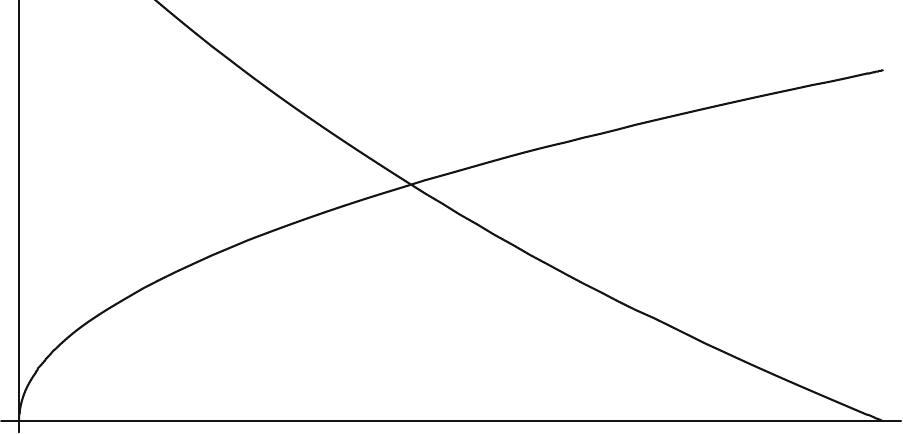
\includegraphics[width=.72\textwidth]{figures/figure-5-2.png}
  \caption{求解匹配条件:情形 1.}
  \label{fig:square-well-matching-case1}
\end{figure}

\begin{figure}[htbp]
  \centering
  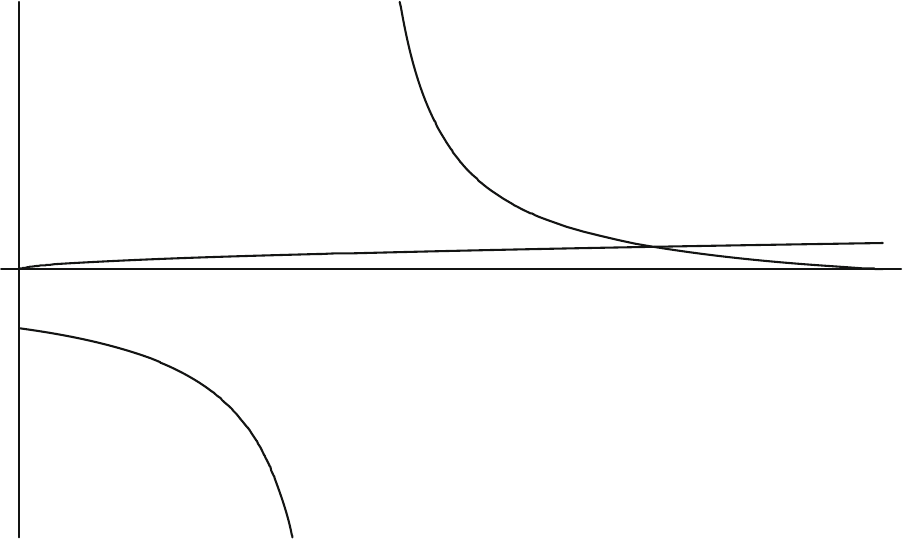
\includegraphics[width=.72\textwidth]{figures/figure-5-3.png}
  \caption{求解匹配条件:情形 2a.}
  \label{fig:square-well-matching-case2a}
\end{figure}

\begin{figure}[htbp]
  \centering
  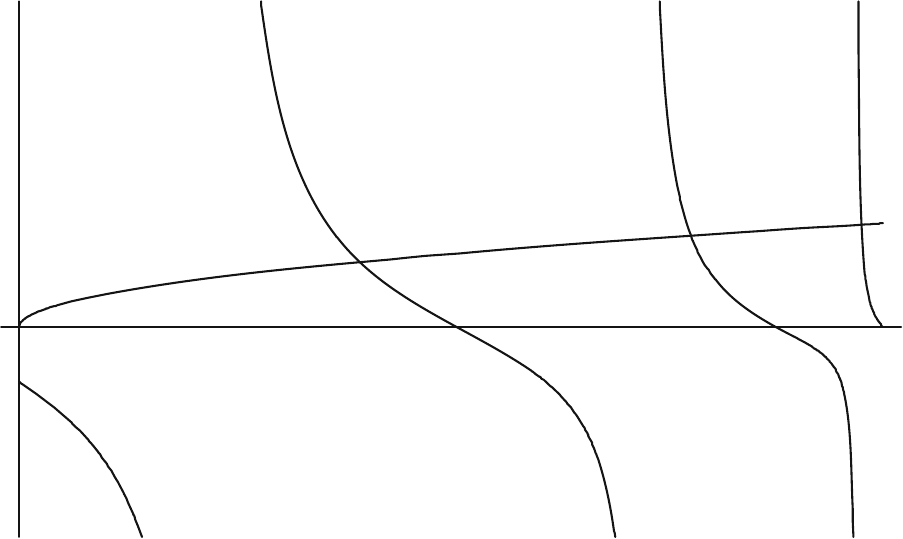
\includegraphics[width=.72\textwidth]{figures/figure-5-4.png}
  \caption{求解匹配条件:情形 2b.}
  \label{fig:square-well-matching-case2b}
\end{figure}

因此,至少找到了一个满足匹配条件的 \(\psi\),它和 \(\psi''\) 都在无穷远处指数衰减.由于该 \(\psi\) 属于 \(\widehat H\) 的定义域,得到如下结果.

\begin{proposition}[方势阱中的偶特征函数]\label{prop:square-well-even-eigenfunction}
对任意正数 \(A,C\),至少存在一个 \(E\in(-C,0)\),使得式~\eqref{eq:square-well-schrodinger} 在 \(\widehat H\) 的定义域中有非零解:
\[
\psi(x)=
\begin{cases}
\cos\left(\sqrt{c-\varepsilon}\,x\right),&-A\le x\le A,\\
\cos\left(\sqrt{c-\varepsilon}\,A\right)
\exp[-\sqrt{\varepsilon}(|x|-A)],&|x|\ge A,
\end{cases}
\]
其中 \(c,\varepsilon\) 由式~\eqref{eq:square-well-parameters} 定义,\(\varepsilon\) 满足式~\eqref{eq:square-well-even-matching}.
\end{proposition}

命题~\ref{prop:square-well-even-eigenfunction} 中没有把 \(\psi\) 归一化为 \(L^{2}(\mathbb{R})\) 中的单位向量,而是将 \(\psi\) 归一化为在原点取值 \(1\).图~\ref{fig:square-well-shallow-ground}--\ref{fig:square-well-deep-excited} 展示了几个例子.浅势阱(\(\sqrt c A=1\))只有一个偶特征向量,即系统基态(具有最小特征值的特征向量).对于深势阱(\(\sqrt c A=30\)),图中还展示了基态和一个激发态(特征值不是最小值的特征向量).

浅势阱中,基态在区间 \([-A,A]\) 外延伸得相当远;深势阱中,基态一离开势阱就很快趋于零.另一方面,图~\ref{fig:square-well-deep-excited} 中的激发态在势阱外延伸得相对较远.

\begin{figure}[htbp]
  \centering
  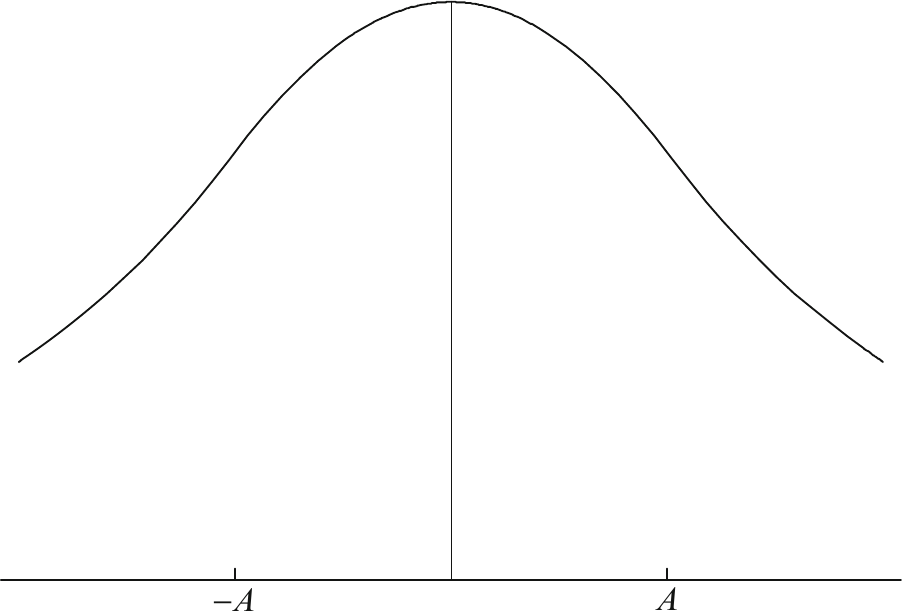
\includegraphics[width=.72\textwidth]{figures/figure-5-5.png}
  \caption{浅势阱的基态.}
  \label{fig:square-well-shallow-ground}
\end{figure}
\begin{figure}[htbp]
  \centering
  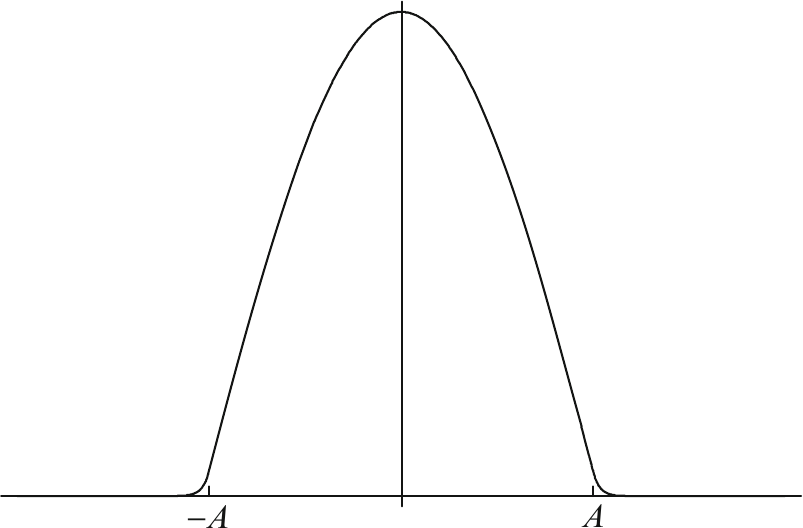
\includegraphics[width=.72\textwidth]{figures/figure-5-6.png}
  \caption{深势阱的基态.}
  \label{fig:square-well-deep-ground}
\end{figure}
\begin{figure}[htbp]
  \centering
  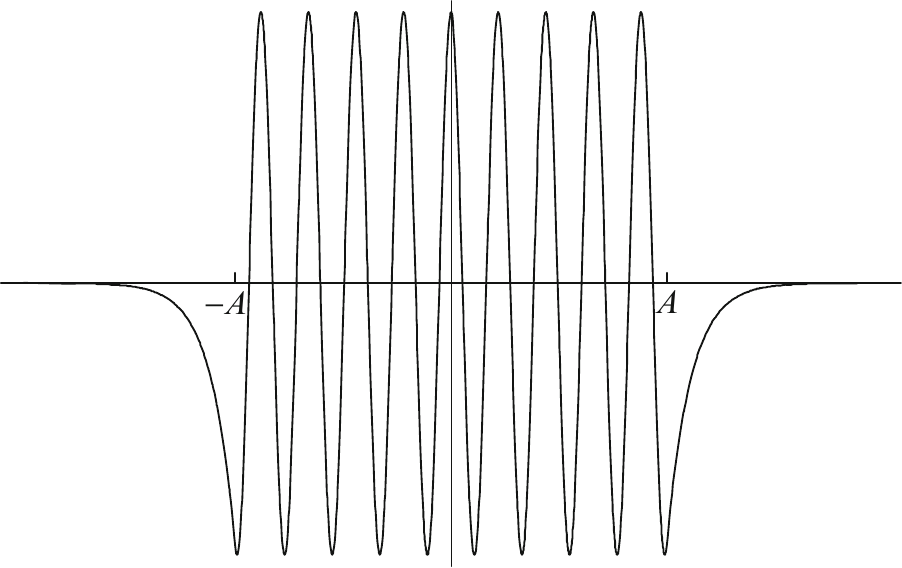
\includegraphics[width=.72\textwidth]{figures/figure-5-7.png}
  \caption{深势阱的激发态.}
  \label{fig:square-well-deep-excited}
\end{figure}

奇解的分析与上述类似.匹配条件~\eqref{eq:square-well-even-matching} 替换为
\begin{equation}
\sqrt{\varepsilon}
=-\sqrt{c-\varepsilon}\cot\left(\sqrt{c-\varepsilon}\,A\right),
\label{eq:square-well-odd-matching}
\end{equation}
(见练习~\ref{ex:square-well-odd-matching}),特征函数公式变为
\[
\psi(x)=
\begin{cases}
\sin\left(\sqrt{c-\varepsilon}\,x\right),&-A\le x\le A,\\
\pm\sin\left(\sqrt{c-\varepsilon}\,A\right)
\exp[-\sqrt{\varepsilon}(|x|-A)],&|x|\ge A,
\end{cases}
\]
其中 \(x>A\) 取正号,\(x<-A\) 取负号.

如果 \(\sqrt c A<\pi/2\),则式~\eqref{eq:square-well-odd-matching} 没有解,因为当 \(\varepsilon\in(0,c)\) 时右端始终为负.当 \(\sqrt c A\) 很大时,式~\eqref{eq:square-well-odd-matching} 会有多个解.典型的匹配情形和相应特征函数见图~\ref{fig:square-well-odd-matching} 与图~\ref{fig:square-well-odd-state}.

\begin{figure}[htbp]
  \centering
  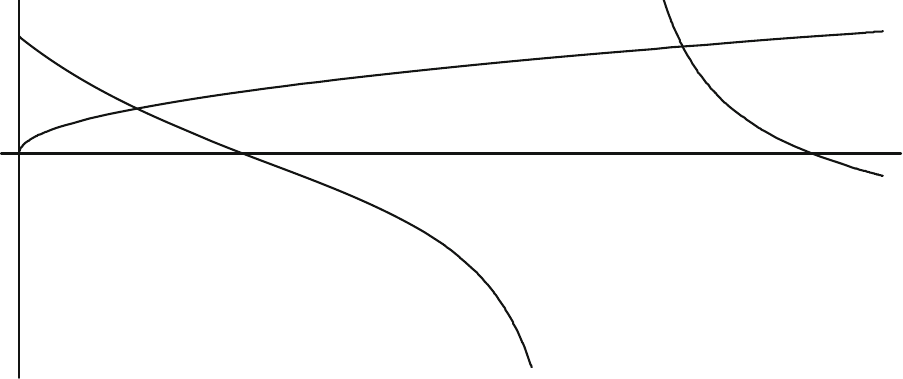
\includegraphics[width=.72\textwidth]{figures/figure-5-8.png}
  \caption{奇解的匹配条件.}
  \label{fig:square-well-odd-matching}
\end{figure}
\begin{figure}[htbp]
  \centering
  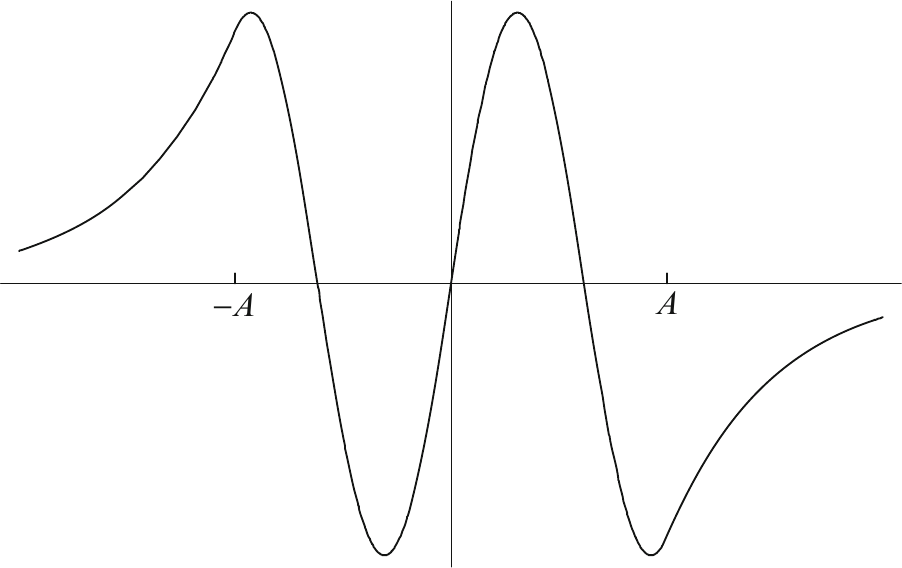
\includegraphics[width=.72\textwidth]{figures/figure-5-9.png}
  \caption{一个奇解.}
  \label{fig:square-well-odd-state}
\end{figure}

\section{隧穿与经典禁戒区域}\label{sec:tunneling}

简要比较经典情形与量子情形.经典地,如果粒子能量为 \(E\),由于动能 \(p^{2}/(2m)\) 总是非负,粒子不可能位于满足 \(V(x)>E\) 的点.于是 \(V(x)\le E\) 的区域称为“经典允许区域”,\(V(x)>E\) 的区域称为“经典禁戒区域”.对方势阱~\eqref{eq:square-well-potential},若 \(-C<E<0\),势阱本身(\(-A\le x\le A\) 的区域)是经典允许区域,而势阱外(\(|x|>A\))是经典禁戒区域.

量子地,若 \(\widehat H\psi=E\psi\),粒子具有确定能量 \(E\).然而,这样的粒子在经典禁戒区域内被发现的概率非零.注意,波函数在经典禁戒区域内虽然不为零,却随其到经典允许区域的距离指数衰减.换言之,量子粒子可以穿透一段距离进入经典禁戒区域.不过,如果 \(E\) 远小于零,即 \(\varepsilon\) 很大,那么满足 \(\widehat H\psi=E\psi\) 的状态在势阱外衰减得非常快,类似于 \(\exp[-\sqrt{\varepsilon}(|x|-A)]\).

更一般地,可以考虑能量近似为 \(E\) 的粒子的含时 Schrödinger 方程.如果要求能量严格等于 \(E\),那么时间依赖并不有趣,因为含时方程的解只是在时间上乘以一个常数相位.可是,我们可以考虑能量不确定度非零但很小的粒子.设粒子在 \(V<E\) 的区域内运动,随后接近 \(V>E\) 的区域(“势垒”).经典地,粒子会从势垒反射并返回;量子地,粒子却可能“隧穿”过势垒,在另一侧出现.也就是说,在稍后的某个时刻,波函数在势垒远侧会有一部分不可忽略的量.

\section{离散谱与连续谱}\label{sec:discrete-continuous-spectrum}

我们对 \(-C<E<0\) 范围内特征值方程~\eqref{eq:square-well-schrodinger} 的分析表明,只有有限多个 \(E\) 值能产生平方可积解.分析 \(E\le-C\) 的情形不难得到:所有非零解至少在一个方向上指数增长(见练习~\ref{ex:square-well-no-low-states}).另一方面,当 \(E>0\) 时,\((-\infty,-A)\) 上的任何解都具有正弦式行为,除非恒等于零,否则不平方可积;根据匹配条件,此时解必须处处为零.

因此,式~\eqref{eq:square-well-schrodinger} 只有有限多个平方可积解(每个解都只确定到常数倍).显然,真正的特征向量——即实际属于 Hilbert 空间 \(L^{2}(\mathbb{R})\) 的特征向量——不可能构成 \(L^{2}(\mathbb{R})\) 的标准正交基.不过,谱定理(第~7 章)会提供某种类似于标准正交基分解的表达,把 \(L^{2}(\mathbb{R})\) 中的元素用式~\eqref{eq:square-well-schrodinger} 的解表示.\(L^{2}(\mathbb{R})\) 中的一般元素 \(\psi\) 是两项之和:第一项是 \(\widehat H\) 的真正(\(L^{2}\))特征向量(它们的 \(E<0\))的线性组合;第二项是 \(E>0\) 的不可平方积“广义特征向量”的连续叠加,即积分.

第~9 章将引入(可能无界的)自伴算子 \(A\) 的谱概念:若对每个 \(\varepsilon>0\),都存在 \(A\) 定义域中的单位向量 \(\psi\),使得 \(\|A\psi-\lambda\psi\|<\varepsilon\),则数 \(\lambda\) 属于 \(A\) 的谱.对方势阱的 Hamilton 算子 \(\widehat H\),不难证明每个满足 \(E\ge0\) 的实数都属于 \(\widehat H\) 的谱(见练习~\ref{ex:square-well-spectrum-positive}).

还可以证明,如果 \(E<0\) 不是特征值(即 \(\widehat H\psi=E\psi\) 没有非零 \(L^{2}\) 解),那么 \(E\) 不属于 \(\widehat H\) 的谱.练习~\ref{ex:square-well-spectrum-negative} 暗示了这一结果.因此,\(\widehat H\) 的谱由 \((-C,0)\) 中的有限个点(至少一个)和整个半轴 \([0,\infty)\) 组成.

\section{练习}\label{sec:chapter5-exercises}

\begin{exercise}\label{ex:square-well-domain-distribution}
\begin{enumerate}
\item 设 \(\psi\) 在 \((-\infty,-A)\)、\((-A,A)\) 和 \((A,\infty)\) 上分别光滑,并在 \(x=A\) 与 \(x=-A\) 处 \(\psi,\psi'\) 都连续.证明对任意紧支集光滑函数 \(\chi\),有
\[
\int_{-\infty}^{\infty}\chi''(x)\psi(x)\,\mathrm{d}x
=\int_{-\infty}^{\infty}\chi(x)\psi''(x)\,\mathrm{d}x,
\]
其中若 \(\psi''\) 在 \(x=\pm A\) 处不存在,则不定义这两个点处的 \(\psi''\).(根据定义~\ref{app:def:distribution-derivative},这意味着 \(\psi\) 的分布二阶导数就是函数 \(\psi''\).)提示:取包含 \(\chi\) 支集的区间 \([-R,R]\),其中 \(R>A\),然后分别在 \([-R,-A]\)、\([-A,A]\) 和 \([A,R]\) 上分部积分,并仔细处理边界项.
\item 现在设 \(\psi\) 在上述三个区间上分别光滑,并且 \(\psi,\psi'\) 在 \(x=\pm A\) 处有左右极限,但假设 \(\psi'\) 在 \(x=-A\) 处有间断.证明上式右端必须增加 \(\chi(-A)\) 的某个非零倍数.
\end{enumerate}
\end{exercise}

\begin{exercise}\label{ex:square-well-odd-matching}
验证定态 Schrödinger 方程奇解的匹配条件~\eqref{eq:square-well-odd-matching}.
\end{exercise}

\begin{exercise}\label{ex:square-well-oscillatory}
设 \(\omega\) 是非零实数,\(\psi(x)=a\cos(\omega x)+b\sin(\omega x)\),其中 \(a,b\) 为实数且不同时为零.证明对任意 \(A\in\mathbb{R}\),有
\[
\lim_{B\to+\infty}\int_{A}^{B}\psi(x)^{2}\,\mathrm{d}x=+\infty.
\]
\end{exercise}

\begin{exercise}\label{ex:square-well-spectrum-positive}
设 \(f\) 是区间 \((0,1)\) 上的 \(C^{\infty}\) 函数,且 \(0<x<1/3\) 时 \(f(x)=1\),\(2/3<x<1\) 时 \(f(x)=0\).在 \(\mathbb{R}\) 上定义“截断”函数族 \(\chi_{n}\):
\[
\chi_{n}(x)=
\begin{cases}
0,&|x|\ge n+1,\\
1,&|x|\le n,\\
f(-x-n),&-(n+1)<x<-n,\\
f(x-n),&n<x<n+1.
\end{cases}
\]
给定 \(E>0\),设 \(\psi\) 是式~\eqref{eq:square-well-schrodinger} 的非零解,且 \(\psi,\psi'\) 在 \(x=\pm A\) 连续.令 \(\psi_{n}=\psi\chi_{n}\).证明 \(\psi_{n}\) 属于 \(\widehat H\) 的定义域,并且
\[
\lim_{n\to\infty}\frac{\|\widehat H\psi_{n}-E\psi_{n}\|}{\|\psi_{n}\|}=0.
\]
\begin{note}
第~9 章将看到,这意味着每个 \(E>0\) 的实数都属于算子 \(\widehat H\) 的谱.
\end{note}
\begin{solution}
估计分子时使用 \(\chi_n'\) 和 \(\chi_n''\) 只支集在两个过渡区间这一事实;估计分母时可对 \(\psi\) 的实部和虚部分别使用练习~\ref{ex:square-well-oscillatory}.
\end{solution}
\end{exercise}

\begin{exercise}\label{ex:square-well-spectrum-negative}
设 \(E<0\),并假设式~\eqref{eq:square-well-schrodinger} 不存在 \(\psi,\psi'\) 连续的非零平方可积解.令 \(\psi\) 是 \(\psi,\psi'\) 在 \(x=\pm A\) 连续的非零解,令 \(\psi_n\) 如练习~\ref{ex:square-well-spectrum-positive}.证明
\[
\frac{\|\widehat H\psi_{n}-E\psi_{n}\|}{\|\psi_{n}\|}
\]
不趋于零.
\end{exercise}

\begin{exercise}\label{ex:square-well-no-low-states}
\begin{enumerate}
\item 证明,当 \(E<-C\) 时,式~\eqref{eq:square-well-schrodinger} 不存在 \(\psi,\psi'\) 连续的非零平方可积解.
\item 对 \(E=-C\) 得到同样的结论.
\end{enumerate}
\begin{note}
分别分析偶解与奇解.
\end{note}
\end{exercise}

\begin{exercise}\label{ex:square-well-ground-state}
把方势阱中粒子的基态定义为具有最低(最负)特征值的特征向量,它对应于最大的 \(\varepsilon\) 值.
\begin{enumerate}
\item 证明基态总是偶函数,即证明满足式~\eqref{eq:square-well-even-matching} 的最大 \(\varepsilon\) 总大于式~\eqref{eq:square-well-odd-matching} 的任何解.
\item 证明基态是处处非零的函数.
\end{enumerate}
\end{exercise}

\chapter{谱定理的若干观点}\label{chap:perspectives-spectral}

\section{无限维情形的困难}\label{sec:spectral-infinite-difficulties}

设 \(A\) 是自伴的 \(n\times n\) 矩阵,即 \(A_{kj}=\overline{A_{jk}}\).线性代数中的标准结果断言:存在 \(\mathbb{C}^{n}\) 的标准正交基 \(\{v_{j}\}_{j=1}^{n}\) 以及实数 \(\lambda_{1},\ldots,\lambda_{n}\),使得 \(Av_{j}=\lambda_{j}v_{j}\).(见文献~[24] 第~8 章定理 18 及第~7 章练习 4.)

用与基无关的语言,可以表述同样的结果:设 \(\mathcal{H}\) 是有限维 Hilbert 空间,\(A\) 是其上的自伴线性算子,即对所有 \(\phi,\psi\in\mathcal{H}\),
\[
\langle\phi,A\psi\rangle=\langle A\phi,\psi\rangle.
\]
那么 \(\mathcal{H}\) 存在一个由 \(A\) 的、具有实特征值的特征向量组成的标准正交基.

由于一般 Hilbert 空间也有标准正交基的标准概念,我们可能希望无限维 Hilbert 空间上的自伴算子也有类似结果.不过,简单例子说明,自伴算子可能根本没有特征向量.比如取 \(\mathcal{H}=L^{2}([0,1])\),定义
\begin{equation}
(A\psi)(x)=x\psi(x).
\label{eq:spectral-position-example}
\end{equation}
则 \(A\) 满足 \(\langle\phi,A\psi\rangle=\langle A\phi,\psi\rangle\),但没有特征向量.因为若 \(x\psi(x)=\lambda\psi(x)\),则 \(\psi\) 必须支集在 \(x=\lambda\) 的集合上,而这个集合的测度为零.因此只有 \(L^{2}([0,1])\) 的零元素满足 \(A\psi=\lambda\psi\).

物理学家会说,算子 \(A\) 确实有特征向量,即分布 \(\delta(x-\lambda)\)(见附录~\ref{app:def:distribution}).这些分布满足 \(x\delta(x-\lambda)=\lambda\delta(x-\lambda)\),但不属于 Hilbert 空间 \(L^{2}([0,1])\).这类属于比 \(\mathcal{H}\) 更大空间的“特征向量”称为广义特征向量.虽然广义特征向量并不实际属于 Hilbert 空间,我们仍可能希望在某种意义下它们形成类似标准正交基的对象.第~\ref{sec:momentum-spectral-example} 节将给出这种“基”如何工作的例子.

顺便提及,对于紧自伴算子,这种关于真正特征向量标准正交基的朴素期待确实成立.Hilbert 空间上的算子 \(A\) 称为紧的,是指 \(A\) 对每个有界集的像都有紧闭包;见文献~[34] 第 I 卷定理 VI.16.不过,量子力学中感兴趣的算子并不紧.(当然,即使自伴算子不紧,它仍可能有特征向量标准正交基,例如量子谐振子的 Hamilton 算子,见第~11 章.)

无限维情形中的自伴算子还会带来另一个严重困难.量子力学中的大多数自伴算子都是无界的,即不存在常数 \(C\),使得对所有 \(\psi\) 有 \(\|A\psi\|\le C\|\psi\|\).例如,考虑 \(L^{2}(\mathbb{R})\) 上的位置算子 \(X\),\((X\psi)(x)=x\psi(x)\).若 \(\mathbf{1}_{E}\) 表示集合 \(E\) 的示性函数,则对每个正整数 \(n\),
\[
\|X\mathbf{1}_{[n,n+1]}\|
\ge n\|\mathbf{1}_{[n,n+1]}\|,
\]
所以 \(X\) 不可能有界.再利用闭图定理与第~9.3 节的初等结果可以证明:若 \(A\) 定义在整个 \(\mathcal{H}\) 上,并且对所有 \(\phi,\psi\in\mathcal{H}\) 满足 \(\langle\phi,A\psi\rangle=\langle A\phi,\psi\rangle\),则 \(A\) 必有界.因此,无界自伴算子不可能定义在整个 \(\mathcal{H}\) 上.

于是,我们把 Hilbert 空间 \(\mathcal{H}\) 上的“无界算子”定义为:从 \(\mathcal{H}\) 的稠密子空间——称为 \(A\) 的定义域——到 \(\mathcal{H}\) 的线性算子.此类算子的自伴性比有界情形复杂得多.显然的条件,即对定义域中的所有 \(\phi,\psi\) 要求 \(\langle\phi,A\psi\rangle=\langle A\phi,\psi\rangle\),并不是“正确”条件;具体地说,这个条件不足以保证谱定理适用于 \(A\).相反,对于任意无界算子 \(A\),我们将定义它的伴随 \(A^{*}\),这是一个有自己的定义域的无界算子.无界算子称为自伴,是指 \(A\) 与 \(A^{*}\) 的定义域相同,且它们在共同定义域上相等.也就是说,自伴性不仅要求 \(A\) 与 \(A^{*}\) 在二者都有定义的地方相等,还要求二者的定义域一致.

\section{谱理论的目标}\label{sec:spectral-goals}

在进入谱理论的细节之前,先想一想我们希望谱定理为我们做什么.首先,我们希望谱定理允许我们把各种函数应用到算子上.例如,我们已经看到,可以令 \(\psi(t)=\exp(-it\widehat H/\hbar)\psi_{0}\) 来“求解”含时 Schrödinger 方程.由于 Hamilton 算子 \(\widehat H\) 无界,使用幂级数定义指数并不方便.不过,如果 \(\widehat H\) 有由特征向量 \(\{e_{k}\}\) 构成的真正标准正交基,且相应特征值为 \(\lambda_{k}\),则可以把 \(e^{-it\widehat H/\hbar}\) 定义为满足
\[
e^{-it\widehat H/\hbar}e_{k}
=e^{-it\lambda_{k}/\hbar}e_{k}
\]
的唯一有界算子.

如果 \(\widehat H\) 没有真正的特征向量标准正交基,我们希望谱定理为 \(\widehat H\) 提供一种“函数演算”,即把函数(包括指数函数)应用到 \(\widehat H\) 上的规则.这个函数演算应当具有类似于真正特征向量标准正交基情形中的性质.

其次,我们希望谱定理为测量自伴算子 \(A\) 的结果提供概率分布.回忆 \(A\) 有真正的特征向量标准正交基 \(\{e_{j}\}\) 且特征值为 \(\lambda_{j}\) 时的测量概率.基于例题~\ref{ex:eigenbasis-probability},对 \(\mathbb{R}\) 的任意 Borel 集 \(E\),令 \(V_{E}\) 为 \(A\) 的所有特征值位于 \(E\) 中的特征向量的闭线性包,令 \(P_{E}\) 为投影到 \(V_{E}\) 上的正交投影.那么对任意单位向量 \(\psi\),有
\begin{equation}
\operatorname{Prob}_{\psi}(A\in E)=\langle\psi,P_{E}\psi\rangle.
\label{eq:spectral-measurement-probability}
\end{equation}
特别地,如果特征值两两不同,且 \(\psi=\sum_{j}c_{j}e_{j}\),那么观测到 \(\lambda_{j}\) 的概率是 \(|c_{j}|^{2}\),因为 \(P_{\{\lambda_{j}\}}\) 正是投影到 \(e_{j}\) 上的投影.

如果 \(A\) 没有真正的特征向量标准正交基,我们希望谱定理为每个 Borel 集 \(E\subset\mathbb{R}\) 提供一个投影算子 \(P_{E}\),从而像式~\eqref{eq:spectral-measurement-probability} 那样定义概率.这些投影算子称为\emph{谱投影},相应子空间 \(V_{E}\) 称为\emph{谱子空间}.(于是 \(P_{E}\) 是投影到 \(V_{E}\) 上的正交投影.)直观地说,\(V_{E}\) 可以看成所有特征值属于 \(E\) 的广义特征向量的闭线性包.

在谱定理的第一种形式中,这两个目标都将实现:谱投影由投影值测度给出,函数演算由关于该测度的积分给出.虽然从实用角度看,自伴算子的(广义)特征向量并不是最重要的,但我们将使用直积分的概念提供理解这类特征向量的框架.谱定理的第二种形式把 Hilbert 空间 \(\mathcal{H}\) 分解为关于某个测度 \(\mu\) 的直积分,其中积分对象是自伴算子 \(A\) 的广义特征子空间.对于特定特征值 \(\lambda\),广义特征空间实际上不会是 \(\mathcal{H}\) 的子空间,除非 \(\mu(\{\lambda\})>0\).因此,直积分为“不实际属于 Hilbert 空间的特征向量”提供了严格含义.

\section{阅读指南}\label{sec:spectral-reading-guide}

虽然本书的谱理论部分有些地方不可避免地技术性很强,但它经过设计,读者可以按需要掌握多或少的内容.愿意把一些结果先当作事实接受的读者,可以只看第~\ref{sec:position-spectral-example} 节的位置算子和第~\ref{sec:momentum-spectral-example} 节的动量算子例子,把它们作为谱定理如何工作的原型.希望了解更多细节的读者,可以在第~7 章看到有界算子谱定理的两种表述,并在第~9 章了解无界自伴算子的基本内容.希望完整学习本主题的读者,则可以在第~8 章看到有界算子谱定理两种形式的完整证明,并在第~10 章看到无界算子谱定理的完整证明.

\section{位置算子}\label{sec:position-spectral-example}

作为第一个例子,考虑位置算子 \(X\),
\[
(X\psi)(x)=x\psi(x),
\]
它作用在 Hilbert 空间 \(\mathcal{H}=L^{2}(\mathbb{R})\) 上.与第~\ref{sec:spectral-infinite-difficulties} 节中的类似算子一样,\(X\) 没有真正的特征向量,即没有实际属于 \(\mathcal{H}\) 的特征向量.如果把 \(X\) 的广义特征向量看成 \(\delta(x-\lambda)\)(\(\lambda\in\mathbb{R}\)),那么可以合理猜测:谱子空间 \(V_{E}\) 应由那些“支集在” \(E\) 上的函数组成,即在 \(E\) 的补集上几乎处处为零的函数.(\(\lambda\in E\) 的“函数”\(\delta(x-\lambda)\) 的叠加应是一个支集在 \(E\) 上的函数.)

谱投影 \(P_{E}\) 是投影到 \(V_{E}\) 上的正交投影,可以计算为
\[
P_{E}\psi=\mathbf{1}_{E}\psi,
\]
其中 \(\mathbf{1}_{E}\) 是 \(E\) 的示性函数.于是根据式~\eqref{eq:spectral-measurement-probability},
\[
\operatorname{Prob}_{\psi}(X\in E)
=\langle\psi,P_{E}\psi\rangle
=\int_{E}|\psi(x)|^{2}\,\mathrm{d}x.
\]
这正是我们在第~3 章中关于位置概率分布所预期的公式.

再看 \(X\) 的函数演算.如果 \(f(\lambda)=\lambda^{m}\),则 \(f(X)\) 应是 \(X\) 的 \(m\) 次幂,即乘以 \(x^{m}\) 的算子.因此合理的想法是:对任意函数 \(f\),令 \(f(X)\) 为乘以 \(f(x)\) 的算子.特别地,\(e^{iaX}\) 就是乘以 \(e^{iax}\) 的有界算子.

\section{乘法算子}\label{sec:multiplication-operators}

由于位置算子就是乘以函数 \(x\),所以很容易找出其谱子空间并构造其函数演算.更一般地,若 \(\mathcal{H}=L^{2}(X,\mu)\),且 \(h\) 是 \(X\) 上的实值可测函数,则可在 \(L^{2}(X,\mu)\) 上定义乘法算子 \(M_{h}\):
\[
M_{h}\psi=h\psi.
\]
谱子空间可以取为
\[
V_{E}=\{\psi\mid\psi\text{ 支集在 }h^{-1}(E)\text{ 上}\},
\]
函数演算则定义为
\[
f(A)=\text{乘以 }f\circ h\text{ 的算子}.
\]

谱定理的一种形式可以简单表述如下:可分 Hilbert 空间上的自伴算子 \(A\) 与一个乘法算子酉等价.也就是说,存在某个 \(\sigma\)-有限测度空间 \((X,\mu)\) 和某个可测函数 \(h\),使得 \(A\) 与乘以 \(h\) 的算子酉等价.(见定理~\ref{thm:unbounded-spectral-multiplication}.)虽然这种谱定理表述极其容易说明,但其中涉及直积分的轻微修正有时更好;更多信息见第~7.3 节.

\section{动量算子}\label{sec:momentum-spectral-example}

现在看谱定理如何作用于 \(L^{2}(\mathbb{R})\) 上的动量算子
\[
P=-i\hbar\frac{\mathrm{d}}{\mathrm{d}x}.
\]
\(P\) 的“特征向量”是 \(e^{ikx}\),\(k\in\mathbb{R}\),相应特征值为 \(\hbar k\).虽然 \(e^{ikx}\) 不属于 \(L^{2}(\mathbb{R})\),但 Fourier 变换说明,\(L^{2}(\mathbb{R})\) 中的任意函数都可以表示成这些函数的叠加,即连续版本的线性组合.事实上,Fourier 系数 \(\widehat\psi(k)\) 可以写成 \(\psi\) 与 \(e^{ikx}\) 的“内积”:
\[
\widehat\psi(k)
=(2\pi)^{-1/2}\int_{-\infty}^{\infty}e^{-ikx}\psi(x)\,\mathrm{d}x
=(2\pi)^{-1/2}\langle e^{ikx},\psi\rangle_{L^{2}(\mathbb{R})},
\]
只需忽略 \(e^{ikx}\) 实际不属于 \(L^{2}\) 这一事实.

实际上,物理学家经常断言 \(e^{ikx}/\sqrt{2\pi}\) 构成 \(L^{2}(\mathbb{R})\) 的“连续意义下的标准正交基”.连续意义下的正交归一,意味着在标准正交集定义中用 Dirac \(\delta\) 函数替换通常的 Kronecker delta:
\begin{equation}
\left\langle\frac{e^{ikx}}{\sqrt{2\pi}},\frac{e^{ilx}}{\sqrt{2\pi}}\right\rangle_{L^{2}(\mathbb{R})}
=\delta(k-l).
\label{eq:continuous-orthogonality}
\end{equation}
这里的 \(\delta\) 应满足,对所有连续函数 \(f\),
\[
\int_{-\infty}^{\infty}f(k)\delta(k-l)\,\mathrm{d}k=f(l).
\]
严格地说,\(\delta(k-l)\) 是一个分布(见附录~\ref{app:def:distribution}).

为式~\eqref{eq:continuous-orthogonality} 赋予某种严格含义,虽然 \(e^{ikx}\) 与 \(e^{ilx}\) 的内积没有定义,但可以用如下表达式近似:
\[
\frac{1}{2\pi}\int_{-A}^{A}e^{-ikx}e^{ilx}\,\mathrm{d}x
=\frac{1}{2\pi}\left.\frac{e^{-i(k-l)x}}{-i(k-l)}\right|_{-A}^{A}
=\frac{\sin[A(k-l)]}{\pi A(k-l)}.
\]
可以证明,把上式看成固定 \(A,l\) 时关于 \(k\) 的函数,当 \(A\to\infty\) 时它表现得像 \(\delta(k-l)\).也就是说,对所有足够良好的 \(\psi\),
\begin{equation}
\lim_{A\to\infty}\int_{-\infty}^{\infty}\psi(k)
\frac{\sin[A(k-l)]}{\pi A(k-l)}\,\mathrm{d}k
=\psi(l).
\label{eq:sinc-delta-limit}
\end{equation}

给出式~\eqref{eq:sinc-delta-limit} 的启发式论证.作变量替换 \(k'=k-l\),可把一般问题化为 \(l=0\).再令 \(\kappa=Ak\),所需结果等价于
\begin{equation}
\lim_{A\to+\infty}\int_{-\infty}^{\infty}
\frac{1}{\pi}\frac{\sin\kappa}{\kappa}f\left(\frac{\kappa}{A}\right)\,\mathrm{d}\kappa
=f(0).
\label{eq:sinc-limit-scaled}
\end{equation}
若可以把极限移入积分,则当 \(A\to\infty\) 时 \(f(\kappa/A)\to f(0)\).因此,只需证明
\begin{equation}
\int_{-\infty}^{\infty}\frac{1}{\pi}\frac{\sin\kappa}{\kappa}\,\mathrm{d}\kappa=1.
\label{eq:sinc-integral}
\end{equation}
虽然式~\eqref{eq:sinc-integral} 中的积分不绝对收敛,却是收敛的广义积分;利用围道积分(或查积分表)可得到其值确实为 \(1\).由于式~\eqref{eq:continuous-orthogonality} 本来就是理解 Fourier 变换的启发式方式,我们不再花时间发展上述论证的严格版本.

利用式~\eqref{eq:continuous-orthogonality},至少形式上可以推导 Fourier 变换的许多标准性质,正如利用 \(L^{2}([0,1])\) 中 \(e^{2\pi inx}\) 的正交归一性可以得到 Fourier 级数的性质.更重要的是,Fourier 变换正是把动量算子变为乘法算子的酉变换.为更清晰地看到这一点,作如下简单缩放.

\begin{definition}[动量波函数]\label{def:momentum-wavefunction}
对任意 \(\psi\in L^{2}(\mathbb{R})\),定义
\[
\widetilde\psi(p)=\frac{1}{\sqrt{\hbar}}\widehat\psi\left(\frac{p}{\hbar}\right),
\]
即
\[
\widetilde\psi(p)=\frac{1}{\sqrt{2\pi\hbar}}
\int_{-\infty}^{\infty}e^{-ipx/\hbar}\psi(x)\,\mathrm{d}x.
\]
函数 \(\widetilde\psi(p)\) 称为与 \(\psi\) 关联的动量波函数.
\end{definition}

根据 Plancherel 定理(定理~\ref{app:thm:plancherel-II})和变量替换,如果 \(\psi\) 是单位向量,那么 \(\widehat\psi\) 和 \(\widetilde\psi\) 也都是单位向量.对于任意单位向量 \(\psi\),我们把 \(|\widetilde\psi(p)|^{2}\) 解释为粒子的动量概率密度,正如 \(|\psi(x)|^{2}\) 是粒子位置概率分布.利用命题~\ref{app:prop:fourier-derivatives},可以直接验证,对足够良好的 \(\psi\),有
\begin{equation}
\widetilde{P\psi}(p)=p\widetilde\psi(p).
\label{eq:momentum-multiplication}
\end{equation}
式~\eqref{eq:momentum-multiplication} 意味着酉映射 \(\psi\mapsto\widetilde\psi\) 把动量算子 \(P\) 变成乘以 \(p\) 的算子.也就是说,在“乘法算子”形式的谱定理中,Fourier 变换(按定义~\ref{def:momentum-wavefunction} 的方式缩放)正好实现了谱定理.

用动量波函数,可以像第~\ref{sec:multiplication-operators} 节那样定义 \(P\) 的谱投影和函数演算.对任意 Borel 集 \(E\subset\mathbb{R}\),定义 \(P_{E}\) 为投影到如下函数空间上的正交投影:\(\widetilde\psi(p)\) 在 \(E\) 外几乎处处为零.若 \(f\) 是 \(\mathbb{R}\) 上任意有界可测函数,则可以定义 \(f(P)\):令 \(f(P)\psi\) 为满足
\[
\widetilde{f(P)\psi}(p)=f(p)\widetilde\psi(p)
\]
的 \(L^{2}(\mathbb{R})\) 中唯一元素.

\chapter{有界自伴算子的谱定理}
\label{chap:bounded-spectral-theorem}
\index{谱定理}
\index{投影值测度}

本章给出有界自伴算子的谱定理.我们先建立有界算子的若干初等性质,然后给出谱定理的两种形式:第一种形式使用投影值测度,第二种形式使用直积分.前一种形式最适合函数演算和测量概率,后一种形式则更接近“广义特征向量”的结构.

\section{有界算子的初等性质}
\label{sec:bounded-operator-properties}

记 \(\mathcal{B}(\mathcal{H})\) 为 Hilbert 空间 \(\mathcal{H}\) 上所有有界线性算子组成的 Banach 空间.对任意 \(A\in\mathcal{B}(\mathcal{H})\),附录~\ref{app:subsec:hilbert} 回顾过存在唯一的算子 \(A^{*}\in\mathcal{B}(\mathcal{H})\),称为 \(A\) 的伴随,满足
\[
\langle\phi,A\psi\rangle=\langle A^{*}\phi,\psi\rangle
\]
对所有 \(\phi,\psi\in\mathcal{H}\) 成立.若 \(A^{*}=A\),则称 \(A\) 为自伴算子.若
\[
\langle\psi,A\psi\rangle\geq 0
\label{eq:bounded-nonnegative}
\]
对所有 \(\psi\in\mathcal{H}\) 成立,则称 \(A\) 为非负算子.

\begin{proposition}[伴随算子的范数]\label{prop:adjoint-norm}
对任意 \(A\in\mathcal{B}(\mathcal{H})\),有
\[
\|A^{*}\|=\|A\|,
\qquad
\|A^{*}A\|=\|A\|^{2}.
\]
特别地,若 \(A\) 自伴,则
\[
\|A^{2}\|=\|A\|^{2}.
\]
\end{proposition}

\begin{proof}
算子范数也可以写成
\[
\|A\|=\sup_{\|\psi\|=1}\|A\psi\|.
\]
另一方面,对任意 \(\phi\in\mathcal{H}\),由 Cauchy--Schwarz 不等式以及取 \(\chi\) 为 \(\phi\) 的适当倍数可得
\[
\|\phi\|=\sup_{\|\chi\|=1}|\langle\chi,\phi\rangle|.
\]
因此
\[
\|A\|=\sup_{\|\phi\|=\|\psi\|=1}|\langle\phi,A\psi\rangle|.
\]
由此得到
\begin{align*}
\|A^{*}\|
&=\sup_{\|\phi\|=\|\psi\|=1}|\langle\phi,A^{*}\psi\rangle|\\
&=\sup_{\|\phi\|=\|\psi\|=1}|\langle A\phi,\psi\rangle|\\
&=\sup_{\|\phi\|=\|\psi\|=1}|\langle\psi,A\phi\rangle|=\|A\|.
\end{align*}
同时,\(\|A^{*}A\|\leq\|A^{*}\|\,\|A\|=\|A\|^{2}\).反过来,
\begin{align*}
\|A^{*}A\|
&=\sup_{\|\phi\|=\|\psi\|=1}|\langle\phi,A^{*}A\psi\rangle|\\
&=\sup_{\|\phi\|=\|\psi\|=1}|\langle A\phi,A\psi\rangle|\\
&\geq\sup_{\|\psi\|=1}|\langle A\psi,A\psi\rangle|=\|A\|^{2}.
\end{align*}
故第二个等式也成立.若 \(A\) 自伴,则 \(A^{*}A=A^{2}\).
\end{proof}

\def\ChapterSevenLater{
\section{有界自伴算子的谱定理(二)}
\label{sec:spectral-theorem-second}

正如第~\ref{sec:multiplication-operators} 节已经指出的,谱定理的一种表述是:每个自伴算子都与一个乘法算子酉等价.对可分 Hilbert 空间上的有界自伴算子 \(A\),这意味着 \(A\) 与 \(L^{2}(X,\mu)\) 上的乘法算子 \(M_{h}\) 酉等价,其中 \((X,\mu)\) 是 \(\sigma\)-有限测度空间,\(h\) 是可测实值函数,且
\[
(M_{h}\psi)(\lambda)=h(\lambda)\psi(\lambda).
\]

虽然乘法算子形式(定理~\ref{thm:spectral-theorem-multiplication})很容易陈述,但还有一种更好的形式,它使用直积分的概念.把取值于 Hilbert 空间 \(\mathcal{H}\) 的 \(L^{2}\) 空间推广到更一般的情形并不困难;在直积分中,我们再向前一步,允许 Hilbert 空间随点而变化.我们从测度空间 \((X,\mu)\) 开始,对每个 \(\lambda\in X\) 给定一个 Hilbert 空间 \(\mathcal{H}_{\lambda}\).直积分中的元素是函数 \(s\),其在每个点的取值 \(s(\lambda)\) 属于 \(\mathcal{H}_{\lambda}\).给定 \(X\) 上的实值可测函数 \(h\),就可以用 \(h\) 乘直积分中的元素 \(s\).

谱定理的直积分形式说,有界自伴算子 \(A\) 与直积分上的乘法算子酉等价.与普通 \(L^{2}\) 空间上的乘法算子相比,直积分有几项优点.第一,集合 \(X\) 与函数 \(h\) 变成规范的:\(X\) 就是 \(A\) 的谱,而 \(h(\lambda)=\lambda\).第二,直积分自带“广义特征向量”的概念,因为 \(\mathcal{H}_{\lambda}\) 可以看成特征值为 \(\lambda\) 的广义特征向量空间.(一般来说,\(\mathcal{H}_{\lambda}\) 并不包含在直积分 Hilbert 空间中;因此,直积分为“不属于算子作用的 Hilbert 空间的特征向量”这一想法提供了严格含义.)第三,直积分给出了按酉等价分类自伴算子的简单方法:两个自伴算子酉等价,当且仅当它们的直积分表示在自然意义下等价(见命题~\ref{prop:bounded-spectral-classification}).

如果只希望得到普通乘法算子版本的简洁结论,那么使用与直积分证明完全相同的方法即可证明它(见定理~\ref{thm:spectral-theorem-multiplication}).不过,对单个自伴算子而言,直积分版本可以说是最完整的谱定理表述.

\subsection{直积分}
\label{subsec:direct-integral}

现在定义直积分.设 \(\mu\) 是集合 \(X\) 上某个 \(\sigma\)-代数 \(\Omega\) 的 \(\sigma\)-有限测度.假设对每个 \(\lambda\in X\),都有一个带内积 \(\langle\cdot,\cdot\rangle_{\lambda}\) 的可分 Hilbert 空间 \(\mathcal{H}_{\lambda}\).我们希望定义关于 \(\mu\) 的 \(\mathcal{H}_{\lambda}\) 的直积分.直积分中的元素将是截面,即函数 \(s\),其值属于这些 Hilbert 空间的并,并满足
\[
s(\lambda)\in\mathcal{H}_{\lambda}
\]
对每个 \(\lambda\in X\) 成立.若右端积分有限,我们希望用
\[
\|s\|^{2}=\int_{X}\langle s(\lambda),s(\lambda)\rangle_{\lambda}\,\mathrm{d}\mu(\lambda)
\]
定义截面 \(s\) 的范数;两个有限范数截面 \(s_{1},s_{2}\) 的内积则应为
\[
\langle s_{1},s_{2}\rangle
:=\int_{X}\langle s_{1}(\lambda),s_{2}(\lambda)\rangle_{\lambda}\,\mathrm{d}\mu(\lambda).
\]

这种描述的问题在于我们还没有说明可测性.由于 \(s(\lambda)\) 对每个 \(\lambda\) 属于不同的空间,直接询问截面 \(s\) 是否可测并没有意义.因此,需要引入额外结构,从而产生可测性的概念.(第一次阅读时,可以把可测性问题看作一个技术细节.)

处理可测性的一种方法,是为每个 \(\mathcal{H}_{\lambda}\) 选择同时的标准正交基.为允许不同空间具有不同维数,我们稍微修改标准正交基的概念:若向量族 \(\{e_{j}\}\) 满足 \(\langle e_{j},e_{k}\rangle=0\)(\(j\neq k\)),每个 \(e_{j}\) 的范数为 0 或 1,且它们张成空间的闭包是整个 \(\mathcal{H}\),就称它为 Hilbert 空间 \(\mathcal{H}\) 的标准正交基.也就是说,我们允许基中的某些向量为零,而非零向量组成通常意义下的标准正交基.

对于 Hilbert 空间族 \(\{\mathcal{H}_{\lambda}\}\),同时标准正交基是截面族 \(\{e_{j}(\cdot)\}_{j=1}^{\infty}\),使得对每个 \(\lambda\),\(\{e_{j}(\lambda)\}_{j=1}^{\infty}\) 是 \(\mathcal{H}_{\lambda}\) 的上述意义下的标准正交基.若函数 \(\lambda\mapsto\dim\mathcal{H}_{\lambda}\) 从 \(X\) 到 \([0,\infty]\) 可测,则可以选择同时标准正交基,使 \(\langle e_{j}(\lambda),e_{k}(\lambda)\rangle_{\lambda}\) 对所有 \(j,k\) 都可测.选定这样的基后,若对每个 \(j\),函数
\[
\lambda\longmapsto\langle e_{j}(\lambda),s(\lambda)\rangle_{\lambda}
\]
都是复值可测函数,就称截面 \(s\) 可测.对基本身的假设意味着每个 \(e_{j}\) 都是可测截面.

把满足上述内积可测条件的同时标准正交基的选择称为 Hilbert 空间族 \(\{\mathcal{H}_{\lambda}\}\) 的可测性结构.若 \(s_{1},s_{2}\) 是两个可测截面,则函数
\[
\lambda\longmapsto\langle s_{1}(\lambda),s_{2}(\lambda)\rangle_{\lambda}
=\sum_{j=1}^{\infty}
\langle s_{1}(\lambda),e_{j}(\lambda)\rangle_{\lambda}
\langle e_{j}(\lambda),s_{2}(\lambda)\rangle_{\lambda}
\]
也是可测函数.

\begin{definition}[Hilbert 空间的直积分]\label{def:direct-integral}
给定以下结构:
\begin{enumerate}
\item \(\sigma\)-有限测度空间 \((X,\Omega,\mu)\);
\item 一个可分 Hilbert 空间族 \(\{\mathcal{H}_{\lambda}\}_{\lambda\in X}\),其维数函数可测;
\item 该 Hilbert 空间族上的可测性结构.
\end{enumerate}
则关于 \(\mu\) 的直积分记作
\[
\int_{X}^{\oplus}\mathcal{H}_{\lambda}\,\mathrm{d}\mu(\lambda),
\]
它是所有满足以下条件的可测截面按几乎处处相等取等价类所得的空间:
\[
\|s\|^{2}:=\int_{X}\langle s(\lambda),s(\lambda)\rangle_{\lambda}\,\mathrm{d}\mu(\lambda)<\infty.
\]
两个截面 \(s_{1},s_{2}\) 的内积定义为
\[
\langle s_{1},s_{2}\rangle
:=\int_{X}\langle s_{1}(\lambda),s_{2}(\lambda)\rangle_{\lambda}\,\mathrm{d}\mu(\lambda).
\]
\end{definition}

为什么两个有限范数截面的内积积分有限？注意
\[
|\langle s_{1}(\lambda),s_{2}(\lambda)\rangle_{\lambda}|
\leq\|s_{1}(\lambda)\|_{\lambda}\|s_{2}(\lambda)\|_{\lambda}.
\]
按假设,\(\|s_{j}(\lambda)\|_{\lambda}\)(\(j=1,2\))是 \(\lambda\) 的平方可积函数,而两个平方可积函数的乘积可积.因此,内积定义中的被积函数也可积.类似于证明 \(L^{2}\) 空间完备性的论证,可以证明 Hilbert 空间的直积分仍是 Hilbert 空间.

直积分构造有两个重要特例.第一,如果每个 \(\mathcal{H}_{\lambda}\) 都只是 \(\mathbb{C}\),那么直积分(带有显然的可测性结构)就是 \(L^{2}(X,\mu)\).第二,若 \(X=\{\lambda_{1},\lambda_{2},\ldots\}\) 是可数集,\(\Omega\) 是 \(X\) 的所有子集组成的 \(\sigma\)-代数,\(\mu\) 是计数测度,则直积分就是 Hilbert 空间直和(定义~\ref{app:def:hilbert-direct-sum}).

给定一个直积分,假设某个 \(\lambda_{0}\in X\) 的单点集 \(\{\lambda_{0}\}\) 可测,且 \(c:=\mu(\{\lambda_{0}\})>0\).则可以把 \(\mathcal{H}_{\lambda_{0}}\) 等距嵌入直积分:将 \(\psi\in\mathcal{H}_{\lambda_{0}}\) 映到截面
\[
s(\lambda)=
\begin{cases}
c^{-1/2}\psi,&\lambda=\lambda_{0},\\
0,&\lambda\neq\lambda_{0}.
\end{cases}
\]
即使 \(\mu(\{\lambda_{0}\})=0\),我们仍可把 \(\mathcal{H}_{\lambda_{0}}\) 看成直积分的某种“广义子空间”.

\begin{theorem}[谱定理:第二种形式]\label{thm:spectral-theorem-direct-integral}
若 \(A\in\mathcal{B}(\mathcal{H})\) 自伴,则在 \(\sigma(A)\) 上存在 \(\sigma\)-有限测度 \(\mu\)、直积分
\[
\int_{\sigma(A)}^{\oplus}\mathcal{H}_{\lambda}\,\mathrm{d}\mu(\lambda),
\]
以及从 \(\mathcal{H}\) 到该直积分的酉映射 \(U\),使得对直积分中的所有截面 \(s\),
\[
\bigl[UAU^{-1}s\bigr](\lambda)=\lambda s(\lambda).
\label{eq:spectral-theorem-direct-integral}
\]
\end{theorem}

定理~\ref{thm:spectral-theorem-direct-integral} 的证明将在下一章与第一种谱定理的证明一同给出.现在先解释它的含义.可以把酉映射 \(U\) 看成将原 Hilbert 空间 \(\mathcal{H}\) 识别为关于 \(A\) 的谱的某个直积分.在这种识别下,自伴算子 \(A\) 变成乘以 \(\lambda\) 的算子,即把截面 \(s(\lambda)\) 送到 \(\lambda s(\lambda)\) 的映射.粗略地说,在这个识别下,\(A\) 在每个空间 \(\mathcal{H}_{\lambda}\) 上都像 \(\lambda I\) 那样作用.因此,可以把每个 \(\mathcal{H}_{\lambda}\) 看成 \(A\) 对应于谱点 \(\lambda\) 的“特征空间”.当然,除非 \(\mu(\{\lambda\})>0\),Hilbert 空间 \(\mathcal{H}_{\lambda}\) 并不真正包含在 \(\mathcal{H}\) 中;不过仍可把其中元素视为 \(A\) 的“广义特征向量”.

直积分形式很容易导出有界自伴算子的分类结果(见本节后面的命题~\ref{prop:bounded-spectral-classification}).与此同时,正如前面提到的,定理~\ref{thm:spectral-theorem-direct-integral} 的证明方法也会给出普通 \(L^{2}\) 空间上乘法算子形式的谱定理.

\begin{theorem}[谱定理:乘法算子形式]\label{thm:spectral-theorem-multiplication}
设 \(A\in\mathcal{B}(\mathcal{H})\) 自伴.则存在 \(\sigma\)-有限测度空间 \((X,\mu)\)、有界可测实值函数 \(h\) 以及酉映射 \(U:\mathcal{H}\to L^{2}(X,\mu)\),使得对所有 \(\psi\in L^{2}(X,\mu)\),
\[
\bigl[UAU^{-1}(\psi)\bigr](\lambda)=h(\lambda)\psi(\lambda).
\]
\end{theorem}

回到谱定理的直积分表述.它给出了函数演算的简单描述.

\begin{proposition}[直积分中的函数演算]\label{prop:direct-integral-functional-calculus}
设 \(A\in\mathcal{B}(\mathcal{H})\) 自伴,\(U\) 是定理~\ref{thm:spectral-theorem-direct-integral} 中的酉映射.则对 \(\sigma(A)\) 上任意有界可测函数 \(f\),有
\[
\bigl[Uf(A)U^{-1}(s)\bigr](\lambda)=f(\lambda)s(\lambda).
\label{eq:direct-integral-functional-calculus}
\]
\end{proposition}

因此,粗略地说,\(f(A)\) 在每个“广义特征空间” \(\mathcal{H}_{\lambda}\) 上等于 \(f(\lambda)I\).当 \(f\) 是多项式时,命题~\ref{prop:direct-integral-functional-calculus} 直接由式~\eqref{eq:spectral-theorem-direct-integral} 得到;连续函数的情形由一致极限得到;一般函数则可用第~8 章的极限论证,尤其是其中的练习 3,得到.

下面讨论第二种谱定理应当具有怎样的唯一性.存在一个“平凡”的非唯一性来源:某些 \(\mathcal{H}_{\lambda}\) 可能是零空间.令 \(E_{0}\) 为满足 \(\dim\mathcal{H}_{\lambda}=0\) 的 \(\lambda\) 的集合.即使 \(\mu(E_{0})>0\),\(E_{0}\) 也不会对截面的范数产生贡献,因为每个截面在 \(E_{0}\) 上自动为零.因此可以定义新测度
\[
\widetilde{\mu}(E)=\mu(E\cap E_{0}^{c}),
\]
它在 \(E_{0}^{c}\) 上与 \(\mu\) 一致,在 \(E_{0}\) 上为零.关于 \(\mu\) 和关于 \(\widetilde{\mu}\) 的直积分是“无法区分的”.所以总可以修改直积分,使 \(\mu\)-几乎处处都有 \(\dim\mathcal{H}_{\lambda}>0\).

另一方面,与定理~\ref{thm:spectral-theorem-first} 中的投影值测度 \(\mu_{A}\) 不同,定理~\ref{thm:spectral-theorem-direct-integral} 中的普通测度 \(\mu\) 并非唯一,而只在等价意义下唯一.这里两个给定可测空间上的 \(\sigma\)-有限测度等价,是指它们有完全相同的零测集.给定 \(\mu\) 后,Hilbert 空间 \(\mathcal{H}_{\lambda}\) 只在酉等价意义下唯一,也就是说,唯一确定的只是各空间的维数.甚至 \(\dim\mathcal{H}_{\lambda}\) 也只在一个 \(\mu\)-零集之外唯一.事实证明,本段及上一段中所述的非唯一性来源就是全部非唯一性来源.

\begin{proposition}[定理~\ref{thm:spectral-theorem-direct-integral} 的唯一性]\label{prop:direct-integral-uniqueness}
设 \(A\in\mathcal{B}(\mathcal{H})\) 自伴,考虑定理~\ref{thm:spectral-theorem-direct-integral} 的两个不同直积分表示:第一个使用测度 \(\mu^{(1)}\) 和 Hilbert 空间 \(\mathcal{H}_{\lambda}^{(1)}\),第二个使用测度 \(\mu^{(2)}\) 和 Hilbert 空间 \(\mathcal{H}_{\lambda}^{(2)}\).若对 \(j=1,2\),\(\dim\mathcal{H}_{\lambda}^{(j)}>0\) 对 \(\mu^{(j)}\)-几乎处处的 \(\lambda\) 成立,则 \(\mu^{(1)}\) 与 \(\mu^{(2)}\) 互相绝对连续,并且
\[
\dim\mathcal{H}_{\lambda}^{(1)}=\dim\mathcal{H}_{\lambda}^{(2)}
\]
对 \(\mu^{(j)}\)-几乎处处的 \(\lambda\) 成立(\(j=1,2\)).
\end{proposition}

本唯一性结果的证明概要见下一章末尾.

应把定理~\ref{thm:spectral-theorem-direct-integral} 看成此前形式(定理~\ref{thm:spectral-theorem-first})的细化.事实上,给定可测集 \(E\subset\sigma(A)\),令 \(V_{E}\) 为所有支集在 \(E\) 上的截面(即在 \(E^{c}\) 上 \(\mu\)-几乎处处为零的截面)的等价类组成的空间.显然这是一个闭子空间.令 \(P_{E}\) 为投影到 \(V_{E}\) 上的正交投影,并定义
\[
\mu_{A}(E)=U^{-1}P_{E}U.
\label{eq:direct-integral-pvm}
\]
不难验证,\(\mu_{A}\) 是以 \(\mathcal{B}(\mathcal{H})\) 中算子为值的投影值测度,并且
\[
\int_{\sigma(A)}\lambda\,\mathrm{d}\mu_{A}(\lambda)=A.
\]

注意,关于 \(A\) 的两个谱定理版本都涉及测度:第一种是投影值测度 \(\mu_{A}\),第二种是取非负实数值的普通测度 \(\mu\).下面的结果说明这两个测度之间的关系.

\begin{proposition}[两种谱测度的零集]\label{prop:spectral-measures-equivalence}
设 \(A\in\mathcal{B}(\mathcal{H})\) 自伴,\(\mu_{A}\) 是定理~\ref{thm:spectral-theorem-first} 给出的投影值测度,\(\mu\) 是定理~\ref{thm:spectral-theorem-direct-integral} 中的实值测度.若 \(\dim\mathcal{H}_{\lambda}>0\) 对 \(\mu\)-几乎处处成立,则对任意 Borel 集 \(E\subset\sigma(A)\),
\[
\mu_{A}(E)=0\quad\Longleftrightarrow\quad\mu(E)=0.
\]
\end{proposition}

这里 \(\mu_{A}(E)=0\) 中的 0 是零算子,而 \(\mu(E)=0\) 中的 0 是实数.不过可以把命题~\ref{prop:spectral-measures-equivalence} 理解为说,\(\mu_{A}\) 与 \(\mu\) 在通常的测度论意义下等价,即具有完全相同的零测集.

\begin{proof}
如前所述,给定定理~\ref{thm:spectral-theorem-direct-integral} 中的直积分,可以通过式~\eqref{eq:direct-integral-pvm} 构造投影值测度;该投影值测度满足
\[
\int_{\sigma(A)}\lambda\,\mathrm{d}\mu_{A}(\lambda)=A.
\]
由定理~\ref{thm:spectral-theorem-first} 的唯一性,它必须就是该定理中的 \(\mu_{A}\).

若 \(\mu(E)=0\),则支集在 \(E\) 上的任意截面几乎处处为零,因而表示直积分中的零元素.此时 \(V_{E}=\{0\}\),由式~\eqref{eq:direct-integral-pvm} 得 \(\mu_{A}(E)=0\).反之,若 \(\mu(E)>0\),由于 \(\mu\) 是 \(\sigma\)-有限的,\(E\) 含有可测子集 \(F\),满足 \(0<\mu(F)<\infty\).令 \(\{e_{j}(\cdot)\}\) 为直积分的可测性结构,并定义
\[
s(\lambda)=
\begin{cases}
\displaystyle\sum_{j=1}^{\infty}2^{-j}e_{j}(\lambda),&\lambda\in F,\\
0,&\lambda\in F^{c}.
\end{cases}
\]
则
\[
\langle s(\lambda),e_{j}(\lambda)\rangle_{\lambda}
=2^{-j}\langle e_{j}(\lambda),e_{j}(\lambda)\rangle_{\lambda}\mathbf{1}_{F}(\lambda),
\]
对每个 \(j\) 都是可测函数,所以 \(s\) 可测.由 \(\mathcal{H}_{\lambda}\) 在 \(\mu\)-几乎处处非零的假设,\(s\) 在 \(F\) 上几乎处处非零,因而范数为正.又因 \(\|s(\lambda)\|\leq1\),且 \(F\) 的测度有限,\(s\) 的范数有限.因此 \(V_{E}\neq\{0\}\),从而 \(\mu_{A}(E)\neq0\).
\end{proof}

若 \(A_{1},A_{2}\) 分别作用在 Hilbert 空间 \(\mathcal{H}_{1},\mathcal{H}_{2}\) 上,若存在酉映射 \(U:\mathcal{H}_{1}\to\mathcal{H}_{2}\),使得
\[
A_{2}=UA_{1}U^{-1},
\]
则称 \(A_{1},A_{2}\) 酉等价.利用命题~\ref{prop:direct-integral-uniqueness},可以给出可分 Hilbert 空间上有界自伴算子按酉等价的分类.对给定的有界自伴算子 \(A\),称函数
\[
\lambda\longmapsto\dim\mathcal{H}_{\lambda}
\]
为 \(A\) 的重数函数.它与直积分分解的选择无关,除了可能在一个零测集上不同.事实证明,有界自伴算子在酉等价意义下由三项数据刻画:作为集合的谱 \(\sigma(A)\)、定理~\ref{thm:spectral-theorem-direct-integral} 中测度 \(\mu\) 的等价类,以及重数函数.

\begin{proposition}[有界自伴算子的分类]\label{prop:bounded-spectral-classification}
设 \(A_{1},A_{2}\) 分别是可分 Hilbert 空间 \(\mathcal{H}_{1},\mathcal{H}_{2}\) 上的有界自伴算子.为它们分别选择定理~\ref{thm:spectral-theorem-direct-integral} 中的直积分表示,并要求 \(\dim\mathcal{H}_{\lambda}>0\) 对相应测度 \(\mu_{j}\)-几乎处处成立(\(j=1,2\)).则 \(A_{1},A_{2}\) 酉等价,当且仅当:
\begin{enumerate}
\item \(\sigma(A_{1})=\sigma(A_{2})\);
\item \(\mu_{1},\mu_{2}\) 互相绝对连续;
\item \(A_{1},A_{2}\) 的重数函数除一个零测集外相同.
\end{enumerate}
\end{proposition}

证明见练习~\ref{ex:prove-spectral-classification}.

\section{练习}
\label{sec:chapter7-exercises}

\begin{exercise}[同时特征向量]\label{ex:simultaneous-eigenvector}
设 \(A,B\) 是作用在非零有限维向量空间上的可交换线性算子.
\begin{enumerate}[label=(\alph*)]
\item 证明 \(A\) 的每个特征子空间在 \(B\) 下不变;
\item 证明 \(A,B\) 至少有一个同时特征向量,即存在非零向量 \(v\) 及常数 \(\lambda,\mu\in\mathbb{C}\),使得 \(Av=\lambda v\),\(Bv=\mu v\).
\end{enumerate}
\end{exercise}

\begin{exercise}[正规算子的特征向量]\label{ex:normal-eigenvector-adjoint}
设 \(A\in\mathcal{B}(\mathcal{H})\) 是正规算子,即 \(AA^{*}=A^{*}A\).若对某个 \(\psi\in\mathcal{H}\) 和 \(\lambda\in\mathbb{C}\),有 \(A\psi=\lambda\psi\),证明 \(A^{*}\psi=\overline{\lambda}\psi\).

\emph{提示:}计算 \(\|(A^{*}-\overline{\lambda}I)\psi\|\).
\end{exercise}

\begin{exercise}[不变子空间的正交补]\label{ex:invariant-orthogonal-complement}
设 \(V\) 是 \(\mathcal{H}\) 的闭子空间,并且在有界算子 \(A\) 下不变,即对所有 \(\psi\in V\),都有 \(A\psi\in V\).证明 \(V^{\perp}\) 在 \(A^{*}\) 下不变.
\end{exercise}

\begin{exercise}[有限维正规算子的标准正交基]\label{ex:finite-normal-orthonormal-basis}
\begin{enumerate}[label=(\alph*)]
\item 设 \(\mathcal{H}\) 是复有限维 Hilbert 空间,\(A\) 是练习~\ref{ex:normal-eigenvector-adjoint} 意义下的正规算子.证明存在由 \(A\) 与 \(A^{*}\) 的同时特征向量组成的 \(\mathcal{H}\) 的标准正交基.
\emph{提示:}使用练习~\ref{ex:simultaneous-eigenvector} 和练习~\ref{ex:invariant-orthogonal-complement}.
\item 设 \(A\) 是复有限维 Hilbert 空间上的线性算子,并假设存在由 \(A\) 的特征向量组成的标准正交基.证明 \(A\) 与 \(A^{*}\) 相交换.
\end{enumerate}
\end{exercise}

\begin{exercise}[逆算子的伴随]\label{ex:adjoint-inverse}
设 \(A\in\mathcal{B}(\mathcal{H})\) 在 \(\mathcal{B}(\mathcal{H})\) 中有逆 \(A^{-1}\).证明
\[
(A^{-1})^{*}A^{*}=A^{*}(A^{-1})^{*}=I.
\]
推出 \(A^{*}\) 可逆,且 \((A^{*})^{-1}=(A^{-1})^{*}\).
\end{exercise}

\begin{exercise}[酉算子的谱]\label{ex:unitary-spectrum}
设 \(U\) 是 \(\mathcal{H}\) 上的酉算子(定义~\ref{app:def:unitary}).证明 \(U\) 的谱包含于单位圆.

\emph{提示:}将 \(U-\lambda I\) 写成 \((-\lambda)(I-U/\lambda)\) 或 \(U(I-\lambda U^{-1})\),证明所有满足 \(|\lambda|\neq1\) 的 \(\lambda\) 都属于预解集.(原文提示中的算子应为 \(U\),而不是 \(\lambda\).)
\end{exercise}

\begin{exercise}[非负算子的谱]\label{ex:nonnegative-spectrum}
设 \(A\in\mathcal{B}(\mathcal{H})\) 自伴且非负,即满足式~\eqref{eq:bounded-nonnegative}.证明 \(A\) 的谱包含于区间 \([0,\infty)\).

\begin{note}
反过来,若 \(A\) 自伴且 \(\sigma(A)\subset[0,\infty)\),则 \(A\) 非负;见第~8 章练习 2.
\end{note}
\end{exercise}

\begin{exercise}[可逆性的稳定性]\label{ex:invertibility-stability}
设 \(A\in\mathcal{B}(\mathcal{H})\) 可逆.证明存在 \(\varepsilon>0\),使得对满足 \(\|B-A\|<\varepsilon\) 的所有 \(B\in\mathcal{B}(\mathcal{H})\),\(B\) 也可逆.

\emph{提示:}使用与命题~\ref{prop:spectrum-basic} 证明中相同的幂级数方法.
\end{exercise}

\begin{exercise}[自伴算子预解算子的范数]\label{ex:selfadjoint-resolvent-norm}
假设 \(A\in\mathcal{B}(\mathcal{H})\) 自伴.
\begin{enumerate}[label=(\alph*)]
\item 若 \(\lambda_{0}\in\mathbb{C}\) 属于 \(A\) 的预解集,证明
\[
\|(A-\lambda_{0}I)^{-1}\|
=\frac{1}{d(\lambda_{0},\sigma(A))},
\qquad
d(\lambda_{0},\sigma(A)):=\inf_{\lambda\in\sigma(A)}|\lambda-\lambda_{0}|.
\]
\emph{提示:}把 \((A-\lambda_{0}I)^{-1}\) 看成 \(A\) 的函数演算中的函数.
\item 给定 \(\lambda_{0}\in\mathbb{C}\),假设存在非零 \(\psi\in\mathcal{H}\),使得
\[
\|A\psi-\lambda_{0}\psi\|<\varepsilon\|\psi\|.
\]
证明存在 \(\lambda\in\sigma(A)\),使得 \(|\lambda-\lambda_{0}|<\varepsilon\).
\end{enumerate}
\end{exercise}

\begin{exercise}[正交投影的乘积]\label{ex:pvm-orthogonality}
设 \(V_{1},V_{2}\) 是 \(\mathcal{H}\) 的两个闭子空间,\(P_{1},P_{2}\) 是相应的正交投影.证明 \(V_{1}\perp V_{2}\) 当且仅当 \(P_{1}P_{2}=0\).
\end{exercise}

\begin{exercise}[投影值测度的交集]\label{ex:pvm-intersection}
设 \(\mu\) 是 \((X,\Omega)\) 上的投影值测度.证明对任意 \(E_{1},E_{2}\in\Omega\),\(\mu(E_{1})\mu(E_{2})\) 是投影到闭子空间
\[
\operatorname{Range}(\mu(E_{1}))\cap\operatorname{Range}(\mu(E_{2}))
\]
上的投影.

\emph{提示:}将 \(E_{1}\) 写为 \(E_{1}=(E_{1}\cap E_{2})\cup(E_{1}\setminus E_{2})\),并使用练习~\ref{ex:pvm-orthogonality}.
\end{exercise}

\begin{exercise}[证明谱分类定理]\label{ex:prove-spectral-classification}
证明命题~\ref{prop:bounded-spectral-classification}.

\emph{提示:}使用命题~\ref{prop:direct-integral-uniqueness} 和 Radon--Nikodym 定理(定理~\ref{app:thm:radon-nikodym}).
\end{exercise}

}

\begin{proposition}[值域与伴随的核]\label{prop:range-kernel-adjoint}
对任意 \(A\in\mathcal{B}(\mathcal{H})\),有
\[
\bigl[\operatorname{Range}(A)\bigr]^{\perp}=\ker(A^{*}).
\]
\end{proposition}

\begin{proof}
若 \(\psi\in[\operatorname{Range}(A)]^{\perp}\),则对所有 \(\phi\in\mathcal{H}\),
\[
0=\langle\psi,A\phi\rangle=\langle A^{*}\psi,\phi\rangle.
\label{eq:range-kernel-proof}
\]
于是 \(A^{*}\psi=0\),即 \(\psi\in\ker(A^{*})\).反过来,若 \(\psi\in\ker(A^{*})\),则式~\eqref{eq:range-kernel-proof} 从右向左读出,说明 \(\psi\) 与每个形如 \(A\phi\) 的向量正交.因此 \(\psi\in[\operatorname{Range}(A)]^{\perp}\).
\end{proof}

下面定义有界算子的谱;它在无限维情形中扮演有限维线性代数中特征值集合的角色.

\begin{definition}[谱与预解集]\label{def:spectrum-resolvent}
对 \(A\in\mathcal{B}(\mathcal{H})\),若 \(\lambda\in\mathbb{C}\) 使得算子 \(A-\lambda I\) 有有界逆,则称 \(\lambda\) 属于 \(A\) 的预解集,记作 \(\rho(A)\).\(A\) 的谱 \(\sigma(A)\) 定义为预解集在 \(\mathbb{C}\) 中的补集.对预解集中的 \(\lambda\),算子 \((A-\lambda I)^{-1}\) 称为 \(\lambda\) 处的预解算子.
\end{definition}

这里说 \(A-\lambda I\) 有有界逆,是指存在有界算子 \(B\),使得
\[
(A-\lambda I)B=B(A-\lambda I)=I.
\]
如果 \(A\) 有界,且 \(A-\lambda I\) 是一一映射并将 \(\mathcal{H}\) 映到整个 \(\mathcal{H}\),那么由闭图定理(定理~\ref{app:thm:closed-graph})可知其逆映射必然有界.因此,\(\rho(A)\) 也可以描述为所有使 \(A-\lambda I\) 既一一又满射的 \(\lambda\) 所组成的集合.

\begin{proposition}[有界算子的谱]\label{prop:spectrum-basic}
对任意 \(A\in\mathcal{B}(\mathcal{H})\),有:
\begin{enumerate}
\item \(\sigma(A)\) 是 \(\mathbb{C}\) 中非空、闭且有界的集合;
\item 若 \(|\lambda|>\|A\|\),则 \(\lambda\in\rho(A)\).
\end{enumerate}
\end{proposition}

\begin{lemma}[Neumann 级数]\label{lem:neumann-series}
若 \(X\in\mathcal{B}(\mathcal{H})\) 满足 \(\|X\|<1\),则 \(I-X\) 可逆,且其逆由 \(\mathcal{B}(\mathcal{H})\) 中收敛的级数给出:
\[
(I-X)^{-1}=I+X+X^{2}+X^{3}+\cdots.
\label{eq:neumann-series}
\]
\end{lemma}

\begin{proof}
由算子范数的次乘性,有 \(\|X^{m}\|\leq\|X\|^{m}\).因此式~\eqref{eq:neumann-series} 右端的几何级数绝对收敛,从而在 Banach 空间 \(\mathcal{B}(\mathcal{H})\) 中收敛(见附录~\ref{app:subsec:banach}).在级数两侧乘以 \(I-X\) 后,除 \(I\) 外的各项全部相消,故其和就是 \(I-X\) 的逆.
\end{proof}

\begin{proof}[命题~\ref{prop:spectrum-basic} 的证明]
对任意非零 \(\lambda\in\mathbb{C}\),写成
\[
A-\lambda I=-\lambda\left(I-\frac{A}{\lambda}\right).
\]
若 \(|\lambda|>\|A\|\),则 \(\|A/\lambda\|<1\),由引理~\ref{lem:neumann-series},\(I-A/\lambda\) 可逆,从而 \(A-\lambda I\) 可逆,且
\[
(A-\lambda I)^{-1}
=-\frac{1}{\lambda}\left(I+\frac{A}{\lambda}+\frac{A^{2}}{\lambda^{2}}+\cdots\right).
\label{eq:resolvent-neumann}
\]
这证明了第二点,并说明 \(\sigma(A)\) 有界.

现在设 \(\lambda_{0}\in\rho(A)\).对另一个 \(\lambda\in\mathbb{C}\),有
\[
A-\lambda I=(A-\lambda_{0}I)\left(I-(\lambda-\lambda_{0})(A-\lambda_{0}I)^{-1}\right).
\label{eq:resolvent-local-factorization}
\]
若
\[
|\lambda-\lambda_{0}|<\frac{1}{\|(A-\lambda_{0}I)^{-1}\|},
\]
则式~\eqref{eq:resolvent-local-factorization} 右端的两个因子都可逆,所以 \(A-\lambda I\) 也可逆.这说明预解集是开集,谱是闭集.

最后证明谱非空.由式~\eqref{eq:resolvent-local-factorization} 可得,在 \(\lambda_{0}\) 附近
\[
\begin{aligned}
(A-\lambda I)^{-1}
&=\left(I-(\lambda-\lambda_{0})(A-\lambda_{0}I)^{-1}\right)^{-1}(A-\lambda_{0}I)^{-1}\\
&=\sum_{m=0}^{\infty}(\lambda-\lambda_{0})^{m}
\bigl((A-\lambda_{0}I)^{-1}\bigr)^{m}(A-\lambda_{0}I)^{-1}.
\end{aligned}
\label{eq:resolvent-local-series}
\]
因此,对任意 \(\phi,\psi\in\mathcal{H}\),函数
\[
\lambda\longmapsto\langle\phi,(A-\lambda I)^{-1}\psi\rangle
\label{eq:resolvent-holomorphic}
\]
在预解集上全纯;并且由式~\eqref{eq:resolvent-neumann},当 \(|\lambda|\to\infty\) 时它趋于零.

若 \(\sigma(A)\) 为空,则式~\eqref{eq:resolvent-holomorphic} 在整个 \(\mathbb{C}\) 上全纯且在无穷远处趋于零.根据 Liouville 定理,它恒为零,对所有 \(\phi,\psi\) 都如此,因而 \((A-\lambda I)^{-1}\) 是零算子;但这不可能,因为
\[
(A-\lambda I)(A-\lambda I)^{-1}=I.
\]
故谱非空.
\end{proof}

注意,若 \(A\psi=\lambda\psi\),其中 \(\psi\neq0\),则 \(A-\lambda I\) 有非零核,所以 \(\lambda\in\sigma(A)\).因此,任何特征值都属于谱.不过在无限维情形中,反过来未必成立:谱中的点可能不是特征值.对于有界自伴算子,谱仍可以用一种与有限维情形相当接近的方式刻画.

\begin{proposition}[有界自伴算子的谱刻画]\label{prop:selfadjoint-spectrum-characterization}
若 \(A\in\mathcal{B}(\mathcal{H})\) 自伴,则:
\begin{enumerate}
\item \(\sigma(A)\subset\mathbb{R}\);
\item 对 \(\lambda\in\mathbb{R}\),\(\lambda\in\sigma(A)\) 当且仅当存在一列 \(\mathcal{H}\) 中的非零向量 \(\psi_{n}\),使得
\[
\lim_{n\to\infty}\frac{\|A\psi_{n}-\lambda\psi_{n}\|}{\|\psi_{n}\|}=0.
\label{eq:almost-eigenvalue}
\]
\end{enumerate}
\end{proposition}

命题中的第二点说,\(\lambda\) 属于谱,当且仅当它是一个“几乎特征值”:存在非零 \(\psi\),使得 \(A\psi\) 等于 \(\lambda\psi\) 加上一个相对于 \(\psi\) 的大小可以任意小的误差.

\begin{lemma}[自伴算子的下界估计]\label{lem:selfadjoint-resolvent-estimate}
若 \(A\in\mathcal{B}(\mathcal{H})\) 自伴,且 \(\lambda=a+ib\in\mathbb{C}\),则
\[
\langle(A-\lambda I)\psi,(A-\lambda I)\psi\rangle
\geq b^{2}\langle\psi,\psi\rangle.
\label{eq:selfadjoint-resolvent-estimate}
\]
\end{lemma}

\begin{proof}
直接计算得
\begin{align*}
&\langle(A-(a+ib)I)\psi,(A-(a+ib)I)\psi\rangle\\
&=\langle(A-aI)\psi,(A-aI)\psi\rangle
 +ib\langle\psi,(A-aI)\psi\rangle
 -ib\langle(A-aI)\psi,\psi\rangle
 +b^{2}\langle\psi,\psi\rangle.
\end{align*}
由于 \(A-aI\) 自伴,右端第二项和第三项相消.因此
\[
\langle(A-\lambda I)\psi,(A-\lambda I)\psi\rangle
=\langle(A-aI)\psi,(A-aI)\psi\rangle+b^{2}\langle\psi,\psi\rangle,
\]
从而得到所需不等式.
\end{proof}

\begin{proof}[命题~\ref{prop:selfadjoint-spectrum-characterization} 的证明]
先证第一点.设 \(\lambda=a+ib\),且 \(b\neq0\).由引理~\ref{lem:selfadjoint-resolvent-estimate},\(A-\lambda I\) 是单射.由命题~\ref{prop:range-kernel-adjoint},
\[
\operatorname{Range}(A-\lambda I)^{\perp}=\ker(A-\overline{\lambda}I).
\]
因为 \(\overline{\lambda}\) 也有非零虚部,\(A-\overline{\lambda}I\) 是单射,故 \(A-\lambda I\) 的值域在 \(\mathcal{H}\) 中稠密.取任意 \(\phi\in\mathcal{H}\),令 \(\phi_{n}=(A-\lambda I)\psi_{n}\) 是值域中的向量列,且 \(\phi_{n}\to\phi\).对 \(\psi_{n}-\psi_{m}\) 使用引理中的估计,得到 \(\{\psi_{n}\}\) 是 Cauchy 列.因此 \(\psi_{n}\to\psi\);由于 \(A\) 有界,
\[
(A-\lambda I)\psi=\lim_{n\to\infty}(A-\lambda I)\psi_{n}=\lim_{n\to\infty}\phi_{n}=\phi.
\]
故 \(A-\lambda I\) 一一且满射.上述估计也说明其逆有界(也可使用闭图定理),所以 \(\lambda\in\rho(A)\).于是谱包含于实轴.

再证第二点.若存在式~\eqref{eq:almost-eigenvalue} 中的向量列,且 \(A-\lambda I\) 有逆,令 \(\phi_{n}=(A-\lambda I)\psi_{n}\),则 \(\psi_{n}=(A-\lambda I)^{-1}\phi_{n}\),从而
\[
\lim_{n\to\infty}\frac{\|\phi_{n}\|}{\|(A-\lambda I)^{-1}\phi_{n}\|}=0,
\]
这说明 \((A-\lambda I)^{-1}\) 实际上无界,矛盾.因此 \(A-\lambda I\) 没有有界逆.

反过来,若不存在满足式~\eqref{eq:almost-eigenvalue} 的向量列,则存在 \(\varepsilon>0\),使得对所有 \(\psi\in\mathcal{H}\),
\[
\|(A-\lambda I)\psi\|\geq\varepsilon\|\psi\|.
\label{eq:selfadjoint-lower-bound}
\]
于是 \(A-\lambda I\) 是单射;并且它是自伴算子,由命题~\ref{prop:range-kernel-adjoint},其值域稠密.利用式~\eqref{eq:selfadjoint-lower-bound},像前面的论证一样可知其值域也是闭集,因而等于整个 \(\mathcal{H}\).所以 \(A-\lambda I\) 有有界逆.
\end{proof}

\begin{example}[乘法算子的谱]\label{ex:multiplication-spectrum}
令 \(\mathcal{H}=L^{2}([0,1])\),定义
\[
(A\psi)(x)=x\psi(x).
\]
则 \(A\) 有界且自伴,并且
\[
\sigma(A)=[0,1].
\]
如第~\ref{sec:spectral-infinite-difficulties} 节所述,\(A\) 没有真正的特征向量.
\end{example}

\begin{proof}
显然 \(\|A\psi\|\leq\|\psi\|\),并且对所有 \(\phi,\psi\in\mathcal{H}\),有 \(\langle\phi,A\psi\rangle=\langle A\phi,\psi\rangle\),故 \(A\) 有界且自伴.给定 \(\lambda\in(0,1)\),考虑
\[
\psi_{n}:=\mathbf{1}_{[\lambda,\lambda+1/n]}.
\]
当 \(n\) 足够大时,\(\|\psi_{n}\|^{2}=1/n\).另一方面,在区间 \([\lambda,\lambda+1/n]\) 上有 \(|x-\lambda|\leq1/n\),所以
\[
\|(A-\lambda I)\psi_{n}\|^{2}\leq\frac{1}{n^{3}}.
\]
由命题~\ref{prop:selfadjoint-spectrum-characterization},\(\lambda\in\sigma(A)\).这对所有 \(\lambda\in(0,1)\) 都成立,而谱是闭集,故 \(\sigma(A)\supset[0,1]\).反之,若 \(\lambda\notin[0,1]\),则函数 \(1/(x-\lambda)\) 在 \([0,1]\) 上有界,\(A-\lambda I\) 的逆就是乘以该函数的算子.因此 \(\sigma(A)=[0,1]\).
\end{proof}

\section{有界自伴算子的谱定理(一)}
\label{sec:spectral-theorem-first}

\subsection{谱子空间}
\label{subsec:spectral-subspaces}

给定一个有界(暂时如此)自伴算子 \(A\),我们希望把每个 Borel 集 \(E\subset\sigma(A)\) 关联到 \(\mathcal{H}\) 的一个闭子空间 \(V_{E}\).直观上,\(V_{E}\) 应当是特征值属于 \(E\) 的广义特征向量所张成的闭子空间.我们希望这些子空间满足:
\begin{enumerate}
\item \(V_{\sigma(A)}=\mathcal{H}\),且 \(V_{\varnothing}=\{0\}\);
\item 若 \(E,F\) 不相交,则 \(V_{E}\perp V_{F}\);
\item 对任意 \(E,F\),有 \(V_{E\cap F}=V_{E}\cap V_{F}\);
\item 若 \(E_{1},E_{2},\ldots\) 两两不相交,且 \(E=\bigcup_{j}E_{j}\),则
\[
V_{E}=\bigoplus_{j}V_{E_{j}};
\]
\item 对任意 \(E\),\(V_{E}\) 在 \(A\) 下不变;
\item 若 \(E\subset[\lambda_{0}-\varepsilon,\lambda_{0}+\varepsilon]\),且 \(\psi\in V_{E}\),则
\[
\|(A-\lambda_{0}I)\psi\|\leq\varepsilon\|\psi\|.
\]
\end{enumerate}
条件 \(V_{\sigma(A)}=\mathcal{H}\) 表达了广义特征向量应张成整个 \(\mathcal{H}\);条件 2 表达了不同特征值对应的广义特征向量仍应具有某种正交性,即使它们并不真正属于 Hilbert 空间.条件 4 中如果出现无穷多个集合,直和取 Hilbert 空间意义下的直和(定义~\ref{app:def:hilbert-direct-sum}).条件 5 和条件 6 则表达了 \(V_{E}\) 由特征值位于 \(E\) 中的广义特征向量构成.

\subsection{投影值测度}
\label{subsec:projection-valued-measures}

用相应的正交投影算子描述 Hilbert 空间的闭子空间很方便.回忆附录~\ref{app:prop:orthogonal-projection}:给定 \(\mathcal{H}\) 的闭子空间 \(V\),存在唯一有界算子 \(P\),它在 \(V\) 上等于恒等算子,在正交补 \(V^{\perp}\) 上等于零.该算子称为投影到 \(V\) 上的正交投影,并满足 \(P^{2}=P\) 及 \(P^{*}=P\).下面的定义把谱子空间的前四个性质(即不涉及算子 \(A\) 的性质)表述为相应正交投影的性质.由于这些性质与测度的性质相似,我们称其为投影值测度.

\begin{definition}[投影值测度]\label{def:projection-valued-measure}
设 \(X\) 是集合,\(\Omega\) 是 \(X\) 上的 \(\sigma\)-代数.若映射 \(\mu:\Omega\to\mathcal{B}(\mathcal{H})\) 满足下列性质,则称其为投影值测度:
\begin{enumerate}
\item 对每个 \(E\in\Omega\),\(\mu(E)\) 都是正交投影;
\item \(\mu(\varnothing)=0\),且 \(\mu(X)=I\);
\item 若 \(E_{1},E_{2},\ldots\in\Omega\) 两两不相交,则对所有 \(v\in\mathcal{H}\),有
\[
\mu\left(\bigcup_{j=1}^{\infty}E_{j}\right)v
=\sum_{j=1}^{\infty}\mu(E_{j})v,
\]
其中级数在 \(\mathcal{H}\) 的范数拓扑中收敛;
\item 对所有 \(E_{1},E_{2}\in\Omega\),有
\[
\mu(E_{1}\cap E_{2})=\mu(E_{1})\mu(E_{2}).
\]
\end{enumerate}
\end{definition}

若 \(E_{1},E_{2}\) 不相交,则定义中的性质 2 和性质 4 告诉我们 \(\mu(E_{1})\mu(E_{2})=0\),由此可知 \(\mu(E_{1})\) 与 \(\mu(E_{2})\) 的值域相互正交(见练习~\ref{ex:pvm-orthogonality}).不难验证,\(\mu(E_{1})\mu(E_{2})\) 是投影到两个值域交集上的投影(见练习~\ref{ex:pvm-intersection}).因此,若对每个 \(E\in\Omega\) 定义闭子空间 \(V_{E}:=\operatorname{Range}(\mu(E))\),则这些 \(V_{E}\) 满足我们对谱子空间预期的前四个性质.

下一小节中,我们将给每个有界自伴算子 \(A\) 关联一个投影值测度 \(\mu_{A}\).此时,投影 \(\mu_{A}(E)\) 可以理解为对应于 \(E\) 的谱子空间上的投影.我们还将引入关于投影值测度的算子值积分;对于与 \(A\) 关联的投影值测度,这个算子值积分正是 \(A\) 的函数演算.

注意,对任意投影值测度 \(\mu\) 和 \(\psi\in\mathcal{H}\),可定义普通的正实值测度 \(\mu_{\psi}\):
\[
\mu_{\psi}(E)=\langle\psi,\mu(E)\psi\rangle.
\label{eq:pvm-scalar-measure}
\]
这就建立了关于投影值测度积分与关于普通测度积分之间的联系.

\begin{proposition}[算子值积分]\label{prop:operator-valued-integration}
设 \(\Omega\) 是集合 \(X\) 上的 \(\sigma\)-代数,\(\mu:\Omega\to\mathcal{B}(\mathcal{H})\) 是投影值测度.则存在唯一的线性映射
\[
f\longmapsto\int_{X}f\,\mathrm{d}\mu
\]
从有界可测复值函数空间映到 \(\mathcal{B}(\mathcal{H})\),使得对所有这样的 \(f\) 以及所有 \(\psi\in\mathcal{H}\),
\[
\left\langle\psi,\left(\int_{X}f\,\mathrm{d}\mu\right)\psi\right\rangle
=\int_{X}f\,\mathrm{d}\mu_{\psi}.
\label{eq:operator-valued-integral-definition}
\]
此外:
\begin{enumerate}
\item 对每个 \(E\in\Omega\),有
\[
\int_{X}\mathbf{1}_{E}\,\mathrm{d}\mu=\mu(E),
\]
特别地,常值函数 1 的积分是 \(I\);
\item 对所有 \(f\),有
\[
\left\|\int_{X}f\,\mathrm{d}\mu\right\|
\leq\sup_{\lambda\in X}|f(\lambda)|;
\label{eq:operator-valued-integral-bound}
\]
\item 积分具有乘法性:
\[
\int_{X}fg\,\mathrm{d}\mu
=\left(\int_{X}f\,\mathrm{d}\mu\right)
 \left(\int_{X}g\,\mathrm{d}\mu\right);
\label{eq:operator-valued-integral-multiplicative}
\]
\item 对所有 \(f\),有
\[
\int_{X}\overline{f}\,\mathrm{d}\mu
=\left(\int_{X}f\,\mathrm{d}\mu\right)^{*}.
\]
特别地,若 \(f\) 为实值函数,则 \(\int_{X}f\,\mathrm{d}\mu\) 自伴.
\end{enumerate}
\end{proposition}

由性质 1 和线性性,投影值测度积分对简单函数具有预期行为.再由性质 2,任意有界可测函数 \(f\) 的积分都可这样计算:取一致收敛于 \(f\) 的简单函数列 \(s_{n}\),则 \(f\) 的积分就是 \(s_{n}\) 的积分在算子范数拓扑中的极限.

积分的乘法性初看起来也许令人惊讶.不过,对任意 \(E_{1},E_{2}\in\Omega\),定义中的性质 3 给出
\[
\left(\int_{X}\mathbf{1}_{E_{1}}\,\mathrm{d}\mu\right)
\left(\int_{X}\mathbf{1}_{E_{2}}\,\mathrm{d}\mu\right)
=\mu(E_{1})\mu(E_{2})=\mu(E_{1}\cap E_{2})
=\int_{X}\mathbf{1}_{E_{1}}\mathbf{1}_{E_{2}}\,\mathrm{d}\mu.
\]
所以,示性函数层面的乘法性已经包含在投影值测度的定义中.

如果试图构造一种实值测度,使相应积分具有乘法性,那么由于 \(\mathbf{1}_{E}^{2}=\mathbf{1}_{E}\),\(\mathbf{1}_{E}\) 的积分,即 \(\mu(E)\),必须满足 \(\mu(E)^{2}=\mu(E)\).这意味着对每个 \(E\),\(\mu(E)\) 只能是 0 或 1.这样的测度确实具有积分的乘法性,但并不有趣.对于算子值测度,\(\mathcal{B}(\mathcal{H})\) 中幂等元(满足 \(A^{2}=A\) 的元素)远多于 \(\mathbb{R}\) 中的幂等元,因此可以得到有趣的乘法性例子.

\begin{proof}[命题~\ref{prop:operator-valued-integration} 的证明]
给定投影值测度 \(\mu\) 和有界可测函数 \(f\),定义 \(Q_{f}:\mathcal{H}\to\mathbb{C}\):
\[
Q_{f}(\psi)=\int_{X}f\,\mathrm{d}\mu_{\psi},
\]
其中 \(\mu_{\psi}\) 由式~\eqref{eq:pvm-scalar-measure} 给出.若 \(f\) 是示性函数,则 \(Q_{f}(\psi)=\langle\psi,\mu(E)\psi\rangle\) 是有界二次型(见定义~\ref{app:def:quadratic-form}).从示性函数到简单函数,再到一般有界可测函数的推广是直接的:对任何有界可测 \(f\),\(Q_{f}\) 都是有界二次型,并满足
\[
|Q_{f}(\psi)|\leq\sup_{\lambda\in X}|f(\lambda)|\,\|\psi\|^{2}.
\label{eq:operator-valued-quadratic-bound}
\]
由命题~\ref{app:prop:quadratic-operator},存在唯一有界算子 \(A_{f}\),使得
\[
Q_{f}(\psi)=\langle\psi,A_{f}\psi\rangle.
\]
定义 \(\int_{X}f\,\mathrm{d}\mu:=A_{f}\),便得到式~\eqref{eq:operator-valued-integral-definition}.线性映射的唯一性来自同一命题中的唯一性.

若 \(f=\mathbf{1}_{E}\),则 \(Q_{f}(\psi)=\mu_{\psi}(E)=\langle\psi,\mu(E)\psi\rangle\),所以相应算子 \(A_{f}=\mu(E)\),这证明了性质 1.性质 2 由式~\eqref{eq:operator-valued-quadratic-bound} 得到.

对于性质 3,我们已经观察到,示性函数层面的乘法性由投影值测度的定义保证.由于式~\eqref{eq:operator-valued-integral-multiplicative} 两边关于 \((\phi,\psi)\) 都是双线性的,它对简单函数成立;再使用性质 2 取极限,即可推广到所有有界可测函数.

最后,若 \(f\) 为实值函数,则 \(Q_{f}(\psi)\) 对所有 \(\psi\) 都是实数.由命题~\ref{app:prop:quadratic-operator},相应算子 \(A_{f}\) 自伴,性质 4 随即由线性性得到.
\end{proof}

\subsection{谱定理}
\label{subsec:spectral-theorem-first-form}

现在可以陈述有界自伴算子谱定理的一种形式.

\begin{theorem}[谱定理:第一种形式]\label{thm:spectral-theorem-first}
若 \(A\in\mathcal{B}(\mathcal{H})\) 自伴,则在 \(\sigma(A)\) 上的 Borel \(\sigma\)-代数存在唯一的投影值测度 \(\mu_{A}\),其值为 \(\mathcal{H}\) 上的投影,并满足
\[
\int_{\sigma(A)}\lambda\,\mathrm{d}\mu_{A}(\lambda)=A.
\label{eq:spectral-theorem-first}
\]
\end{theorem}

由于 \(A\) 的谱有界,函数 \(f(\lambda)=\lambda\) 在 \(\sigma(A)\) 上有界.本定理的证明将在第~8 章给出.

\begin{definition}[函数演算]\label{def:functional-calculus}
设 \(A\in\mathcal{B}(\mathcal{H})\) 自伴,\(f:\sigma(A)\to\mathbb{C}\) 是有界可测函数.令
\[
f(A):=\int_{\sigma(A)}f(\lambda)\,\mathrm{d}\mu_{A}(\lambda),
\label{eq:functional-calculus}
\]
其中 \(\mu_{A}\) 是定理~\ref{thm:spectral-theorem-first} 中的投影值测度,则称 \(f(A)\) 为 \(f\) 在 \(A\) 处的函数演算.
\end{definition}

把 \(\mu_{A}\) 从 \(\sigma(A)\) 延拓到整个 \(\mathbb{R}\),规定 \(\mathbb{R}\setminus\sigma(A)\) 的测度为零.粗略地说,\(f(A)\) 在投影算子 \(\mu_{A}([\lambda,\lambda+\mathrm{d}\lambda))\) 的值域上等于 \(f(\lambda)I\).

由于关于 \(\mu_{A}\) 的积分具有乘法性,由式~\eqref{eq:spectral-theorem-first} 可知,如果 \(f(\lambda)=\lambda^{m}\),其中 \(m\) 是正整数,则 \(f(A)=A^{m}\).进一步地,级数 \(e^{a\lambda}=\sum_{m=0}^{\infty}(a\lambda)^{m}/m!\) 在紧集 \(\sigma(A)\) 上一致收敛,所以由函数 \(f(\lambda)=e^{a\lambda}\) 的函数演算得到的 \(e^{aA}\) 可以用幂级数计算.

\begin{definition}[谱子空间]\label{def:spectral-subspace}
设 \(A\in\mathcal{B}(\mathcal{H})\) 自伴,令 \(\mu_{A}\) 为相应的投影值测度,并将它延拓到 \(\mathbb{R}\),令 \(\mathbb{R}\setminus\sigma(A)\) 的测度为零.对每个 Borel 集 \(E\subset\mathbb{R}\),定义 \(\mathcal{H}\) 的谱子空间为
\[
V_{E}:=\operatorname{Range}(\mu_{A}(E)).
\label{eq:spectral-subspace-definition}
\]
\end{definition}

投影值测度的定义保证这些谱子空间满足第~\ref{subsec:spectral-subspaces} 节列出的前四个性质.下面说明式~\eqref{eq:spectral-theorem-first} 如何给出剩下的两个性质.

\begin{proposition}[谱子空间的性质]\label{prop:spectral-subspace-properties}
若 \(A\in\mathcal{B}(\mathcal{H})\) 自伴,则由 \(A\) 关联的谱子空间满足:
\begin{enumerate}
\item 每个谱子空间 \(V_{E}\) 在 \(A\) 下不变;
\item 若 \(E\subset[\lambda_{0}-\varepsilon,\lambda_{0}+\varepsilon]\),则对所有 \(\psi\in V_{E}\),有
\[
\|(A-\lambda_{0}I)\psi\|\leq\varepsilon\|\psi\|;
\]
\item \(A|_{V_{E}}\) 的谱包含于 \(E\) 的闭包;
\item 若 \(\lambda_{0}\in\sigma(A)\),则对 \(\lambda_{0}\) 的每个邻域 \(U\),都有 \(V_{U}\neq\{0\}\),等价地,\(\mu_{A}(U)\neq0\).
\end{enumerate}
\end{proposition}

\begin{proof}
先证第一点.对 \(\sigma(A)\) 上任意两个有界可测函数 \(f,g\),算子 \(f(A)\) 和 \(g(A)\) 可交换,因为它们按任意次序相乘都等于函数 \(fg=gf\) 的积分.特别地,\(A\)(即函数 \(f(\lambda)=\lambda\) 的积分)与 \(\mu_{A}(E)\)(即示性函数 \(\mathbf{1}_{E}\) 的积分)可交换.因此,对值域中的向量 \(\mu_{A}(E)\phi\),有
\[
A\mu_{A}(E)\phi=\mu_{A}(E)A\phi,
\]
右端仍在 \(\mu_{A}(E)\) 的值域中,故谱子空间不变.

对于第二点,设 \(\psi\in V_{E}\),且 \(E\subset[\lambda_{0}-\varepsilon,\lambda_{0}+\varepsilon]\).则 \(\psi\) 在 \(\mu_{A}(E)\) 的值域中,于是
\[
(A-\lambda_{0}I)\psi=(A-\lambda_{0}I)\mu_{A}(E)\psi.
\]
令 \(f(\lambda)=\lambda-\lambda_{0}\),则 \(\mu_{A}(E)=\mathbf{1}_{E}(A)\),且 \(A-\lambda_{0}I=f(A)\).由积分的乘法性,
\[
(A-\lambda_{0}I)\psi=(f\mathbf{1}_{E})(A)\psi.
\]
因为 \(|f(\lambda)\mathbf{1}_{E}(\lambda)|\leq\varepsilon\),由式~\eqref{eq:operator-valued-integral-bound},算子 \((f\mathbf{1}_{E})(A)\) 的范数至多为 \(\varepsilon\).

对于第三点,若 \(\lambda_{0}\notin\overline{E}\),则函数
\[
g(\lambda)=\frac{\mathbf{1}_{E}(\lambda)}{\lambda-\lambda_{0}}
\]
有界.于是 \(g(A)\) 有界,并且
\[
g(A)(A-\lambda_{0}I)=(A-\lambda_{0}I)g(A)=\mathbf{1}_{E}(A).
\]
这说明 \(g(A)\) 在 \(V_{E}\) 上的限制是 \(A\) 在 \(V_{E}\) 上的限制的逆.因此 \(\lambda_{0}\notin\sigma(A|_{V_{E}})\).

对于第四点,固定 \(\lambda_{0}\in\sigma(A)\).假设对某个 \(\varepsilon>0\),有 \(\mu_{A}((\lambda_{0}-\varepsilon,\lambda_{0}+\varepsilon))=0\).考虑有界函数
\[
f(\lambda)=
\begin{cases}
\dfrac{1}{\lambda-\lambda_{0}},&|\lambda-\lambda_{0}|\geq\varepsilon,\\
0,&|\lambda-\lambda_{0}|<\varepsilon.
\end{cases}
\]
函数 \(f(\lambda)(\lambda-\lambda_{0})\) 除上述区间外恒等于 1;由于该区间的测度为零,它与常值函数 1 在 \(\mu_{A}\)-几乎处处意义下相同.因此由积分的乘法性,
\[
f(A)(A-\lambda_{0}I)=(A-\lambda_{0}I)f(A)=I,
\]
说明 \(f(A)\) 是 \(A-\lambda_{0}I\) 的有界逆,矛盾于 \(\lambda_{0}\in\sigma(A)\).
\end{proof}

\begin{proposition}[与算子相交换的算子]\label{prop:commuting-operator-functional-calculus}
若 \(A\in\mathcal{B}(\mathcal{H})\) 自伴,且 \(B\in\mathcal{B}(\mathcal{H})\) 与 \(A\) 相交换,则:
\begin{enumerate}
\item 对 \(\sigma(A)\) 上任意有界可测函数 \(f\),\(f(A)\) 与 \(B\) 相交换;
\item \(A\) 的每个谱子空间在 \(B\) 下不变.
\end{enumerate}
\end{proposition}

本命题的证明留到第~8 章.到这里,我们至少对有界自伴算子实现了谱定理的一个目标:给出描述自伴算子 \(A\) 在状态 \(\psi\) 中测量概率的概率测度.

\begin{proposition}[测量概率的谱测度]\label{prop:spectral-measurement-probability}
设 \(A\in\mathcal{B}(\mathcal{H})\) 自伴,\(\psi\in\mathcal{H}\) 是单位向量.则存在唯一的 \(\mathbb{R}\) 上概率测度 \(\mu_{\psi}^{A}\),使得对所有非负整数 \(m\),
\[
\int_{\mathbb{R}}\lambda^{m}\,\mathrm{d}\mu_{\psi}^{A}(\lambda)
=\langle\psi,A^{m}\psi\rangle.
\label{eq:moment-spectral-measure}
\]
\end{proposition}

第~9 章将证明无界自伴算子版本的本命题.不过在无界情形,即使 \(\psi\) 属于所有 \(A^{m}\) 的定义域,我们也无法得到概率测度的唯一性;谱定理仍提供一个规范的选择.

\begin{proof}
按第~\ref{subsec:projection-valued-measures} 节的方式,在 \(\sigma(A)\) 上定义
\[
\mu_{\psi}^{A}(E)=\langle\psi,\mu_{A}(E)\psi\rangle.
\]
投影值测度积分的性质给出
\[
\langle\psi,A^{m}\psi\rangle
=\left\langle\psi,\left(\int_{\sigma(A)}\lambda^{m}\,\mathrm{d}\mu_{A}(\lambda)\right)\psi\right\rangle
=\int_{\sigma(A)}\lambda^{m}\,\mathrm{d}\mu_{\psi}^{A}(\lambda).
\]
把 \(\mu_{\psi}^{A}\) 延拓到 \(\mathbb{R}\),在 \(\mathbb{R}\setminus\sigma(A)\) 上令其为零,即得到所需概率测度.又因为
\[
|\langle\psi,A^{m}\psi\rangle|\leq\|\psi\|^{2}\|A^{m}\|\leq\|\psi\|^{2}\|A\|^{m},
\]
其矩至多指数增长,关于矩问题的标准唯一性定理(例如文献~[18] 第 4 章定理 8.1)给出 \(\mu_{\psi}^{A}\) 的唯一性.
\end{proof}

\ChapterSevenLater

\chapter{有界自伴算子谱定理的证明}
\label{chap:bounded-spectral-proofs}

本章证明上一章陈述的谱定理的所有形式.投影值测度形式的证明分为两步.第一步构造连续函数演算:把 \(\sigma(A)\) 上的每个连续函数 \(f\) 关联到一个算子 \(f(A)\).第二步证明这个连续函数演算可以表示为关于投影值测度的积分.

\section{第一种谱定理的证明}
\label{sec:proof-spectral-first}

\subsection{第一阶段:连续函数演算}
\label{subsec:continuous-functional-calculus-proof}

对任意 \(A\in\mathcal{B}(\mathcal{H})\),定义谱半径
\[
R(A):=\sup_{\lambda\in\sigma(A)}|\lambda|.
\]
由命题~\ref{prop:spectrum-basic} 和命题~\ref{prop:selfadjoint-spectrum-characterization},当 \(A\) 自伴时,\(\sigma(A)\) 是 \(\mathbb{R}\) 中非空有界集合.由命题~\ref{prop:spectrum-basic} 的第二点,对任意有界算子都有 \(R(A)\leq\|A\|\).一般来说,\(\|A\|\) 可能远大于 \(R(A)\):例如若 \(A\) 是幂零矩阵,则 \(R(A)=0\),但 \(\|A\|\) 可以任意大.

\begin{lemma}[自伴算子的谱半径]\label{lem:selfadjoint-spectral-radius}
若 \(A\in\mathcal{B}(\mathcal{H})\) 自伴,则
\[
\|A\|=R(A).
\]
\end{lemma}

为证明该引理,先确定命题~\ref{prop:spectrum-basic} 的证明中预解级数的收敛半径.由命题~\ref{prop:adjoint-norm},对任意有界算子有 \(\|A^{*}A\|=\|A\|^{2}\).若 \(A\) 自伴,则
\[
\|A^{2}\|=\|A\|^{2},
\]
迭代可得
\[
\|A^{2^{n}}\|=\|A\|^{2^{n}}.
\label{eq:spectral-radius-power-norm}
\]
考虑有界自伴算子 \(A\) 的形式预解展开
\[
\begin{aligned}
(A-\lambda I)^{-1}
&=-\frac{1}{\lambda}\left(I-\frac{A}{\lambda}\right)^{-1}\\
&=-\sum_{m=0}^{\infty}\frac{A^{m}}{\lambda^{m+1}}.
\end{aligned}
\label{eq:resolvent-series-ch8}
\]
若 \(|\lambda|>\|A\|\),则上一章的证明说明该级数在算子范数拓扑中收敛,且其和确实是 \((A-\lambda I)^{-1}\).反之若 \(|\lambda|\leq\|A\|\),由式~\eqref{eq:spectral-radius-power-norm},级数中相应项的范数不趋于零,所以它不可能在算子范数拓扑中收敛.于是式~\eqref{eq:resolvent-series-ch8} 的收敛半径为 \(\|A\|\).

\begin{proof}[引理~\ref{lem:selfadjoint-spectral-radius} 的证明]
已知 \(R(A)\leq\|A\|\).为证明反向不等式,注意 \((A-\lambda I)^{-1}\) 是定义在 \(|\lambda|>R(A)\) 上的算子值全纯函数,因此其 Laurent 级数必须在 \(|\lambda|>R(A)\) 上收敛.而该 Laurent 级数正是式~\eqref{eq:resolvent-series-ch8},我们已经证明它在 \(|\lambda|\leq\|A\|\) 时发散.若 \(R(A)<\|A\|\),便产生矛盾.

具体地,上一章命题~\ref{prop:spectrum-basic} 的证明中式~\eqref{eq:resolvent-local-series} 表明,\(\lambda\mapsto(A-\lambda I)^{-1}\) 在预解集的每一点附近都可展开为 \(\lambda-\lambda_{0}\) 的收敛幂级数.因此,对任意有界线性泛函 \(\xi\in\mathcal{B}(\mathcal{H})^{*}\),复值函数
\[
\lambda\longmapsto\xi((A-\lambda I)^{-1})
\]
在预解集上全纯,并且有唯一的 Laurent 展开,它由对式~\eqref{eq:resolvent-series-ch8} 逐项施加 \(\xi\) 得到.这个级数在包含于预解集的最大圆环,即 \(|\lambda|>R(A)\) 上收敛.

式~\eqref{eq:resolvent-series-ch8} 收敛意味着,对每个 \(|\lambda|>R(A)\) 以及每个 \(\xi\),数列 \(\{\xi(A^{m}/\lambda^{m+1})\}\) 有界.由一致有界原理(附录~\ref{app:thm:uniform-boundedness} 的推论),集合
\[
\left\{\frac{A^{m}}{\lambda^{m+1}}\right\}_{m=0}^{\infty}
\]
在 Banach 空间 \(\mathcal{B}(\mathcal{H})\) 中有界.特别地,对每个 \(|\lambda|>R(A)\),存在常数 \(C\),使得
\[
\frac{\|A^{2^{n}}\|}{|\lambda|^{2^{n}}}
=\frac{\|A\|^{2^{n}}}{|\lambda|^{2^{n}}}\leq C.
\]
若 \(\|A\|>R(A)\),取 \(R(A)<|\lambda|<\|A\|\) 就会与此不等式矛盾.因此 \(R(A)=\|A\|\).
\end{proof}

下一步是理解多项式作用于自伴算子时谱如何变化.

\begin{lemma}[谱映射定理]\label{lem:polynomial-spectral-mapping}
对任意 \(A\in\mathcal{B}(\mathcal{H})\) 和任意多项式 \(p\),有
\[
\sigma(p(A))=p(\sigma(A)).
\label{eq:polynomial-spectral-mapping}
\]
也就是说,\(p(A)\) 的谱恰好由 \(p(\lambda)\)(其中 \(\lambda\in\sigma(A)\))组成.
\end{lemma}

\begin{proof}
若 \(p\) 为常数,结论显然.设 \(\deg p\geq1\),写
\[
p(z)=a_{n}z^{n}+a_{n-1}z^{n-1}+\cdots+a_{0}.
\]
先证明 \(p(\sigma(A))\subset\sigma(p(A))\).设 \(\lambda\in\sigma(A)\).注意
\[
p(A)-p(\lambda)I
=a_{n}(A^{n}-\lambda^{n}I)+\cdots+a_{1}(A-\lambda I).
\]
又有
\[
A^{k}-\lambda^{k}I
=(A-\lambda I)(A^{k-1}+\lambda A^{k-2}+\cdots+\lambda^{k-1}I).
\]
因此可从 \(p(A)-p(\lambda)I\) 的每一个非零项中提出因子 \(A-\lambda I\),得到
\[
p(A)-p(\lambda)I=(A-\lambda I)q(A),
\]
其中 \(q\) 是某个多项式.由于 \(A-\lambda I\) 不可逆,且它与 \(q(A)\) 相交换,\((A-\lambda I)q(A)\) 不可能可逆(见练习~\ref{ex:noninvertible-product}).所以 \(p(\lambda)\in\sigma(p(A))\).

再证明 \(\sigma(p(A))\subset p(\sigma(A))\).设 \(\gamma\in\sigma(p(A))\).由于 \(\mathbb{C}\) 代数闭,存在复数 \(b_{1},\ldots,b_{n}\),使得
\[
p(z)-\gamma=c(z-b_{1})(z-b_{2})\cdots(z-b_{n}).
\label{eq:polynomial-factorization}
\]
于是
\[
p(A)-\gamma I=c(A-b_{1}I)(A-b_{2}I)\cdots(A-b_{n}I).
\]
左端不可逆,因此右端至少有一个因子不可逆(有限个两两可交换的可逆算子之积若可逆,则每个因子都可逆).所以某个 \(b_{j}\in\sigma(A)\).由式~\eqref{eq:polynomial-factorization},\(p(b_{j})-\gamma=0\),即 \(\gamma=p(b_{j})\).
\end{proof}

最后一步使用 Stone--Weierstrass 定理,说明多项式在 \(C(\sigma(A);\mathbb{R})\)(即 \(\sigma(A)\) 上连续实值函数空间)中关于上确界范数稠密.

\begin{proposition}[连续函数演算]\label{prop:continuous-functional-calculus}
若 \(A\in\mathcal{B}(\mathcal{H})\) 自伴,则存在唯一有界线性映射
\[
C(\sigma(A);\mathbb{R})\longrightarrow\mathcal{B}(\mathcal{H}),\qquad f\longmapsto f(A),
\]
使得当 \(f(\lambda)=\lambda^{m}\) 时,\(f(A)=A^{m}\).该映射称为 \(A\) 的(实值)连续函数演算.
\end{proposition}

\begin{proof}
若 \(A\) 自伴,且 \(p\) 是实值多项式,则 \(p(A)\) 自伴.结合谱映射定理和引理~\ref{lem:selfadjoint-spectral-radius},得到
\[
\|p(A)\|=\sup_{\lambda\in\sigma(A)}|p(\lambda)|.
\label{eq:polynomial-functional-calculus-isometry}
\]
因此 \(p\mapsto p(A)\) 是从 \(\sigma(A)\) 上多项式空间(带上确界范数)到有界算子空间的等距线性映射.由 Stone--Weierstrass 定理,多项式在 \(C(\sigma(A);\mathbb{R})\) 中稠密;再由 BLT 定理(附录~\ref{app:thm:bounded-extension}),该映射唯一延拓为从 \(C(\sigma(A);\mathbb{R})\) 到 \(\mathcal{B}(\mathcal{H})\) 的有界线性映射.
\end{proof}

\begin{proposition}[连续函数演算的性质]\label{prop:continuous-functional-calculus-properties}
若 \(A\in\mathcal{B}(\mathcal{H})\) 自伴,则上述连续函数演算满足:
\begin{enumerate}
\item 乘法性:\((fg)(A)=f(A)g(A)\);
\item 自伴性:对所有 \(f\),\(f(A)\) 自伴;
\item 非负性:若 \(f\geq0\),则 \(f(A)\) 是非负算子;
\item 范数与谱:
\[
\|f(A)\|=\sup_{\lambda\in\sigma(A)}|f(\lambda)|,
\label{eq:continuous-functional-calculus-norm}
\]
且
\[
\sigma(f(A))=\{f(\lambda):\lambda\in\sigma(A)\}.
\label{eq:continuous-functional-calculus-spectrum}
\]
\end{enumerate}
\end{proposition}

\begin{proof}
乘法性对多项式成立,再取一致极限便对所有连续函数成立.若 \(p\) 是实值多项式且 \(A\) 自伴,则 \(p(A)\) 自伴,取极限得到第二点.若 \(f\geq0\),令 \(g=\sqrt{f}\),则 \(g\) 为实值连续函数,且对所有 \(\psi\),
\[
\langle\psi,f(A)\psi\rangle
=\langle\psi,g(A)^{2}\psi\rangle
=\langle g(A)\psi,g(A)\psi\rangle\geq0,
\label{eq:nonnegative-functional-calculus}
\]
故第三点成立.式~\eqref{eq:continuous-functional-calculus-norm} 对多项式已由式~\eqref{eq:polynomial-functional-calculus-isometry} 得到,对一般连续函数取极限即可.

为证明式~\eqref{eq:continuous-functional-calculus-spectrum},先设 \(\lambda_{0}\) 不在 \(f\) 的值域中.则
\[
g(\lambda):=\frac{1}{f(\lambda)-\lambda_{0}}
\]
在 \(\sigma(A)\) 上连续,且 \(g(A)\) 是 \(f(A)-\lambda_{0}I\) 的逆.因此 \(\lambda_{0}\notin\sigma(f(A))\).

反过来,设 \(\lambda_{0}=f(\mu)\),其中 \(\mu\in\sigma(A)\).若 \(f(A)-f(\mu)I\) 可逆,取一致收敛于 \(f\) 的多项式列 \(p_{n}\).根据第~7 章练习~\ref{ex:invertibility-stability},只要算子在范数拓扑中充分接近一个可逆算子,它也可逆.因此对充分大的 \(n\),\(p_{n}(A)-p_{n}(\mu)I\) 必须可逆;这与谱映射定理矛盾.
\end{proof}

\subsection{第二阶段:算子值 Riesz 表示定理}
\label{subsec:operator-valued-riesz}

现在进入谱定理证明的第二阶段.我们使用测度论中的 Riesz 表示定理,而不是 Hilbert 空间连续线性泛函的 Riesz 表示定理.下述形式足够使用.

\begin{theorem}[Riesz 表示定理]\label{thm:measure-riesz-representation}
设 \(X\) 是紧度量空间,\(C(X;\mathbb{R})\) 是连续实值函数空间.若线性泛函 \(\Lambda:C(X;\mathbb{R})\to\mathbb{R}\) 在 \(f\) 的所有取值非负时满足 \(\Lambda(f)\geq0\),则存在唯一的 Borel \(\sigma\)-代数上的正实值测度 \(\mu\),使得
\[
\Lambda(f)=\int_{X}f\,\mathrm{d}\mu
\]
对所有 \(f\in C(X;\mathbb{R})\) 成立.
\end{theorem}

这是有限测度,因为 \(\mu(X)=\Lambda(1)\).关于该定理在实轴紧子集情形的简短证明,可参见文献~[34] 第 I 卷第 353--354 页;完整结果见文献~[12] 定理 7.2 和 7.8.

对于有界自伴算子 \(A\),上一小节构造了映射 \(f\mapsto f(A)\).若 \(f\geq0\),则命题~\ref{prop:continuous-functional-calculus-properties} 的第三点说明 \(f(A)\) 非负.因此对每个 \(\psi\in\mathcal{H}\),定义
\[
\Lambda_{\psi}(f):=\langle\psi,f(A)\psi\rangle.
\]
它满足 Riesz 表示定理的假设,于是对每个 \(\psi\) 存在唯一测度 \(\mu_{\psi}\),使得
\[
\langle\psi,f(A)\psi\rangle
=\int_{\sigma(A)}f(\lambda)\,\mathrm{d}\mu_{\psi}(\lambda)
\label{eq:measure-riesz-functional-calculus}
\]
对所有 \(f\in C(\sigma(A);\mathbb{R})\) 成立.注意
\[
\mu_{\psi}(\sigma(A))=\Lambda_{\psi}(1)=\|\psi\|^{2}.
\label{eq:mu-psi-total-mass}
\]

\begin{definition}[由测度族定义的二次型]\label{def:Qf-measure}
若 \(f\) 是 \(\sigma(A)\) 上的有界可测复值函数,定义 \(Q_{f}:\mathcal{H}\to\mathbb{C}\):
\[
Q_{f}(\psi):=\int_{\sigma(A)}f(\lambda)\,\mathrm{d}\mu_{\psi}(\lambda).
\label{eq:Qf-definition}
\]
\end{definition}

当 \(f\) 是实值连续函数时,\(Q_{f}(\psi)=\langle\psi,f(A)\psi\rangle\),所以 \(Q_{f}\) 是有界二次型.事实证明,对任意有界可测 \(f\),\(Q_{f}\) 都是有界二次型,于是由命题~\ref{app:prop:quadratic-operator} 可把它关联到一个有界算子,仍记作 \(f(A)\).建立这一算子的性质后,我们将通过 \(\mu_{A}(E):=\mathbf{1}_{E}(A)\) 构造所需的投影值测度.

\begin{proposition}[有界可测函数给出的二次型]\label{prop:Qf-quadratic}
对 \(\sigma(A)\) 上任意有界可测函数 \(f\),定义~\ref{def:Qf-measure} 中的 \(Q_{f}\) 都是有界二次型.
\end{proposition}

\begin{proof}
令 \(\mathcal{F}\) 为所有使 \(Q_{f}\) 成为二次型的有界 Borel 可测函数组成的空间.显然 \(\mathcal{F}\) 是复向量空间并包含 \(C(\sigma(A);\mathbb{R})\).它对一致有界的逐点极限封闭,因为由支配收敛定理,\(Q_{f}(\psi)\) 对这样的极限连续.标准测度论方法(见练习~\ref{ex:bounded-borel-generation})表明,\(\mathcal{F}\) 包含所有有界 Borel 可测函数.

另一方面,由式~\eqref{eq:mu-psi-total-mass},
\[
|Q_{f}(\psi)|\leq\sup_{\lambda\in\sigma(A)}|f(\lambda)|\,\|\psi\|^{2},
\]
所以 \(Q_{f}\) 总是有界二次型.
\end{proof}

\begin{definition}[可测函数演算]\label{def:measurable-functional-calculus}
对 \(\sigma(A)\) 上有界可测函数 \(f\),令 \(f(A)\) 为由 \(Q_{f}\) 通过命题~\ref{app:prop:quadratic-operator} 关联的算子,即唯一满足
\[
\langle\psi,f(A)\psi\rangle=Q_{f}(\psi)
=\int_{\sigma(A)}f\,\mathrm{d}\mu_{\psi}
\]
对所有 \(\psi\in\mathcal{H}\) 成立的算子.
\end{definition}

若 \(f\) 为实值函数,则 \(Q_{f}(\psi)\) 对所有 \(\psi\) 为实数,因此相应算子 \(f(A)\) 自伴.下面构造 \(\mu_{A}\) 后将看到,这里的 \(f(A)\) 与定义~\ref{def:functional-calculus} 中的积分完全一致.

\begin{proposition}[可测函数演算的乘法性]\label{prop:measurable-functional-calculus-multiplicative}
对任意两个有界可测函数 \(f,g\),有
\[
(fg)(A)=f(A)g(A).
\label{eq:measurable-functional-calculus-multiplicative}
\]
\end{proposition}

\begin{proof}
令 \(\mathcal{F}_{1}\) 为所有满足
\[
(fg)(A)=f(A)g(A)
\]
对每个 \(g\in C(\sigma(A);\mathbb{R})\) 成立的有界可测函数 \(f\) 所组成的空间.它是复向量空间并包含 \(C(\sigma(A);\mathbb{R})\).由支配收敛定理,\(f\mapsto Q_{f}(\psi)\) 对一致有界的逐点极限连续;再由极化恒等式(命题~\ref{app:prop:polarization}),与 \(Q_{f}\) 关联的半双线性型 \(L_{f}\) 也具有同样的连续性.

由极化恒等式,若对所有 \(\psi\) 及所有连续实值 \(g\),
\[
\langle\psi,(fg)(A)\psi\rangle
=\langle\psi,f(A)g(A)\psi\rangle,
\]
等价地,
\[
Q_{fg}(\psi)=L_{f}(\psi,g(A)\psi),
\]
则 \(f\in\mathcal{F}_{1}\).因此 \(\mathcal{F}_{1}\) 对一致有界逐点极限封闭.由练习~\ref{ex:bounded-borel-generation},它包含所有有界 Borel 可测函数.

再令 \(\mathcal{F}_{2}\) 为所有满足式~\eqref{eq:measurable-functional-calculus-multiplicative}(对所有有界 Borel 可测 \(g\))的有界 Borel 可测函数 \(f\) 所组成的空间.刚才的结论说明 \(\mathcal{F}_{2}\) 包含连续实值函数;对 \(\mathcal{F}_{1}\) 的同一论证说明 \(\mathcal{F}_{2}\) 就是所有有界 Borel 可测函数.
\end{proof}

\begin{theorem}[投影值测度的构造]\label{thm:construct-pvm}
设 \(A\in\mathcal{B}(\mathcal{H})\) 自伴.对 \(\sigma(A)\) 中每个可测集 \(E\),定义
\[
\mu_{A}(E):=\mathbf{1}_{E}(A),
\]
其中 \(\mathbf{1}_{E}(A)\) 由定义~\ref{def:measurable-functional-calculus} 给出.则 \(\mu_{A}\) 是 \(\sigma(A)\) 上的投影值测度,并且
\[
\int_{\sigma(A)}\lambda\,\mathrm{d}\mu_{A}(\lambda)=A.
\label{eq:construct-pvm-integral}
\]
\end{theorem}

该定理证明了第一种谱定理(定理~\ref{thm:spectral-theorem-first})中投影值测度的存在性.

\begin{proof}
由于 \(\mathbf{1}_{E}\) 是实值函数且 \(\mathbf{1}_{E}^{2}=\mathbf{1}_{E}\),命题~\ref{prop:continuous-functional-calculus-properties} 说明 \(\mathbf{1}_{E}(A)\) 自伴且满足 \(\mathbf{1}_{E}(A)^{2}=\mathbf{1}_{E}(A)\).根据附录~\ref{app:prop:orthogonal-projection},它是正交投影.

若 \(E_{1},E_{2}\) 可测,则 \(\mathbf{1}_{E_{1}\cap E_{2}}=\mathbf{1}_{E_{1}}\mathbf{1}_{E_{2}}\),故
\[
\mu_{A}(E_{1}\cap E_{2})=\mu_{A}(E_{1})\mu_{A}(E_{2}).
\]
若 \(E_{1},E_{2},\ldots\) 两两不相交,则不同投影的值域相互正交.令 \(P\) 为投影到包含所有这些值域的最小闭子空间上的投影,则对所有 \(\psi\),
\[
\sum_{j=1}^{\infty}\mu_{A}(E_{j})\psi=P\psi,
\]
其中级数在范数拓扑中收敛.令 \(E=\bigcup_{j}E_{j}\),则
\[
f_{N}:=\sum_{j=1}^{N}\mathbf{1}_{E_{j}}
\]
一致有界(上界为 1),并逐点收敛到 \(\mathbf{1}_{E}\).再次使用式~\eqref{eq:measure-riesz-functional-calculus} 中的支配收敛,得到
\[
\lim_{N\to\infty}\left\langle\psi,\sum_{j=1}^{N}\mathbf{1}_{E_{j}}(A)\psi\right\rangle
=\langle\psi,\mathbf{1}_{E}(A)\psi\rangle.
\]
所以 \(\mathbf{1}_{E}(A)=P\),这就证明了可数可加性.

若 \(f=\mathbf{1}_{E}\),则
\[
\int_{\sigma(A)}f(\lambda)\,\mathrm{d}\mu_{A}(\lambda)=f(A).
\label{eq:integral-equals-functional-calculus}
\]
由线性性,这对简单函数成立;再取极限,对所有有界 Borel 可测函数成立.特别地,当 \(f(\lambda)=\lambda\) 时,积分等于连续函数演算中的 \(f(A)\),而后者对多项式 \(f(\lambda)=\lambda\) 就是 \(A\).故式~\eqref{eq:construct-pvm-integral} 成立.
\end{proof}

现在证明上一章的命题~\ref{prop:commuting-operator-functional-calculus}.

\begin{proof}[命题~\ref{prop:commuting-operator-functional-calculus} 的证明]
若 \(B\) 与 \(A\) 相交换,则 \(B\) 与任意多项式 \(p(A)\) 相交换.按照连续函数演算的构造取极限可知,\(B\) 与任意连续实值函数 \(f(A)\) 相交换.

令 \(\mathcal{F}\) 为所有使 \(f(A)\) 与 \(B\) 相交换的有界 Borel 可测函数 \(f\) 所组成的空间.对任意 \(\phi,\psi\),条件等价于
\[
\langle\phi,f(A)B\psi\rangle=\langle B^{*}\phi,f(A)\psi\rangle,
\]
即
\[
L_{f}(\phi,B\psi)=L_{f}(B^{*}\phi,\psi).
\]
前面已经说明,固定向量后 \(f\mapsto L_{f}\) 对一致有界逐点极限连续.因此 \(\mathcal{F}\) 对这类极限封闭;由练习~\ref{ex:bounded-borel-generation},它包含所有有界 Borel 可测函数.这证明了第一点,第二点则取 \(f=\mathbf{1}_{E}\) 即得.
\end{proof}

\section{第二种谱定理的证明}
\label{sec:proof-spectral-second}

现在证明定理~\ref{thm:spectral-theorem-direct-integral}.先处理 \(A\) 有循环向量的特殊情形,即存在 \(\psi\),使得 \(A^{k}\psi\)(\(k=0,1,2,\ldots\))张成稠密子空间.此时直积分就是一个 \(L^{2}\) 空间,即所有 \(\mathcal{H}_{\lambda}\) 都等于 \(\mathbb{C}\),所以直积分形式与乘法算子形式重合.

\begin{lemma}[循环向量情形]\label{lem:cyclic-spectral-representation}
设 \(A\in\mathcal{B}(\mathcal{H})\) 自伴,\(\psi\) 是 \(A\) 的循环向量.令 \(\mu_{\psi}\) 为定理~\ref{thm:measure-riesz-representation} 给出的唯一测度,使得
\[
\langle\psi,f(A)\psi\rangle
=\int_{\sigma(A)}f(\lambda)\,\mathrm{d}\mu_{\psi}(\lambda)
\]
对所有连续实值函数 \(f\) 成立.则存在酉映射
\[
U:\mathcal{H}\to L^{2}(\sigma(A),\mu_{\psi}),
\]
使得
\[
\bigl[UAU^{-1}\phi\bigr](\lambda)=\lambda\phi(\lambda).
\]
\end{lemma}

\begin{proof}
先在形如 \(p(A)\psi\) 的向量组成的复向量空间上定义 \(U\):
\[
U[p(A)\psi]=p.
\]
写 \(p=p_{1}+ip_{2}\),其中 \(p_{1},p_{2}\) 是实值多项式.由于 \(p_{1}(A),p_{2}(A)\) 自伴且相交换,
\[
\begin{aligned}
\|p(A)\psi\|^{2}
&=\langle\psi,(p_{1}(A)^{2}+p_{2}(A)^{2})\psi\rangle\\
&=\int_{\sigma(A)}(p_{1}(\lambda)^{2}+p_{2}(\lambda)^{2})\,\mathrm{d}\mu_{\psi}(\lambda).
\end{aligned}
\label{eq:cyclic-isometry}
\]
若 \(p(A)\psi=0\),则 \(p\) 在 \(\mu_{\psi}\)-几乎处处为零,故它表示 \(L^{2}\) 中的零元素.因此 \(U\) 定义良好,并且式~\eqref{eq:cyclic-isometry} 说明它在初始定义域上等距.初始定义域包含所有 \(A^{k}\psi\),因而在 \(\mathcal{H}\) 中稠密.由 BLT 定理,\(U\) 唯一延拓为从 \(\mathcal{H}\) 到 \(L^{2}(\sigma(A),\mu_{\psi})\) 的等距映射.由 Stone--Weierstrass 定理及附录中的稠密性结果,多项式在该 \(L^{2}\) 空间中稠密,所以 \(U\) 实际上是酉映射.

由于 \(U\) 把 \(A^{k}\psi\) 映到函数 \(\lambda\mapsto\lambda^{k}\),有 \(UAU^{-1}(\lambda^{k})=\lambda^{k+1}\).因此对所有多项式 \(p\),
\[
\bigl[UAU^{-1}p\bigr](\lambda)=\lambda p(\lambda).
\]
再由多项式在 \(L^{2}\) 中稠密性,结论对所有 \(\phi\in L^{2}\) 成立.
\end{proof}

\begin{lemma}[由投影值测度构造普通测度]\label{lem:pvm-dominating-measure}
设 \(A\in\mathcal{B}(\mathcal{H})\) 自伴,\(\mu_{A}\) 是定理~\ref{thm:construct-pvm} 中的投影值测度.则在 \(\sigma(A)\) 上存在非负实值测度 \(\mu\),使得对所有 Borel 集 \(E\),
\[
\mu_{A}(E)=0\quad\Longleftrightarrow\quad\mu(E)=0.
\]
\end{lemma}

\begin{proof}
取 \(\mathcal{H}\) 的标准正交基 \(\{e_{j}\}\),令
\[
\mu_{e_{j}}(E):=\langle e_{j},\mu_{A}(E)e_{j}\rangle.
\]
因为 \(\mu_{e_{j}}(\sigma(A))=\langle e_{j},Ie_{j}\rangle=1\),定义
\[
\mu:=\sum_{j=1}^{\infty}2^{-j}\mu_{e_{j}}
\]
得到有限测度.若 \(\mu_{A}(E)=0\),则所有 \(\mu_{e_{j}}(E)=0\),所以 \(\mu(E)=0\).反之,若 \(\mu(E)=0\),则对每个 \(j\),
\[
0=\langle e_{j},\mu_{A}(E)e_{j}\rangle
=\langle\mu_{A}(E)e_{j},\mu_{A}(E)e_{j}\rangle,
\]
因为 \(\mu_{A}(E)\) 自伴且幂等.因此 \(\mu_{A}(E)e_{j}=0\) 对所有 \(j\) 成立,得到 \(\mu_{A}(E)=0\).
\end{proof}

\begin{lemma}[循环子空间分解]\label{lem:cyclic-decomposition}
若 \(A\in\mathcal{B}(\mathcal{H})\) 自伴,则 \(\mathcal{H}\) 可以分解为闭的非零子空间 \(W_{j}\) 的正交直和,每个 \(W_{j}\) 在 \(A\) 下不变,且 \(A|_{W_{j}}\) 有循环向量.这样的子空间数目有限或可数无限.
\end{lemma}

\begin{proof}
利用 \(\mathcal{H}\) 可分,取其可数稠密子集 \(\{\phi_{j}\}\).令 \(W_{1}\) 为 \(\phi_{1},A\phi_{1},A^{2}\phi_{1},\ldots\) 张成的闭子空间.它在 \(A\) 下不变,且 \(\psi_{1}:=\phi_{1}\) 是 \(A|_{W_{1}}\) 的循环向量.若 \(W_{1}=\mathcal{H}\),则完成.否则取最小的使 \(\phi_{j}\notin W_{1}\) 的 \(j\),令 \(\psi_{2}\) 为 \(\phi_{j}\) 在 \(W_{1}^{\perp}\) 上的正交投影,并令 \(W_{2}\) 为 \(\psi_{2},A\psi_{2},A^{2}\psi_{2},\ldots\) 的闭线性包.

\(W_{2}\) 在 \(A\) 下不变,\(\psi_{2}\) 是循环向量.由于 \(A\) 自伴且保持 \(W_{1}\) 不变,它也保持 \(W_{1}^{\perp}\) 不变,因此所有 \(A^{k}\psi_{2}\) 都与 \(W_{1}\) 正交,故 \(W_{2}\perp W_{1}\).重复这一过程,得到一族两两正交、在 \(A\) 下不变且各自有循环向量的闭子空间.若过程有限步终止,它们张成 \(\mathcal{H}\);否则,由 \(\{\phi_{j}\}\) 的稠密性,它们的 Hilbert 空间直和仍是整个 \(\mathcal{H}\).
\end{proof}

\begin{proof}[定理~\ref{thm:spectral-theorem-direct-integral} 的证明]
取引理~\ref{lem:cyclic-decomposition} 中的 \(\{W_{j},\psi_{j}\}\),令 \(A_{j}=A|_{W_{j}}\).对每个 \(A_{j}\),由引理~\ref{lem:cyclic-spectral-representation} 得到
\[
U_{j}:W_{j}\to L^{2}(\sigma(A_{j}),\mu_{\psi_{j}}),
\]
使 \(U_{j}A_{j}U_{j}^{-1}\) 是乘以 \(\lambda\) 的算子.为把这些映射拼合起来,需要把它们都改写到同一个测度 \(\mu\) 下.

由练习~\ref{ex:restriction-spectrum},\(\sigma(A_{j})\subset\sigma(A)\).并且若 \(E\subset\sigma(A_{j})\),则 \(\mathbf{1}_{E}(A_{j})\) 等于 \(\mathbf{1}_{E}(A)\) 在 \(W_{j}\) 上的限制.因此 \(\mu_{A}(E)=0\) 会推出 \(\mu_{A_{j}}(E)=0\),进而推出 \(\mu_{\psi_{j}}(E)=0\).取引理~\ref{lem:pvm-dominating-measure} 中的测度 \(\mu\),并把每个 \(\mu_{\psi_{j}}\) 延拓到 \(\sigma(A)\)(在 \(\sigma(A)\setminus\sigma(A_{j})\) 上为零),则 \(\mu_{\psi_{j}}\ll\mu\).由 Radon--Nikodym 定理(附录~\ref{app:thm:radon-nikodym}),存在密度 \(\rho_{j}\),使得 \(\mathrm{d}\mu_{\psi_{j}}=\rho_{j}\,\mathrm{d}\mu\).

映射 \(f\mapsto\rho_{j}^{1/2}f\) 是从 \(L^{2}(\sigma(A_{j}),\mu_{\psi_{j}})\) 到 \(L^{2}(\sigma(A_{j}),\mu)\) 的酉映射.因此定义
\[
(\widetilde U_{j}\psi)(\lambda)=\rho_{j}(\lambda)^{1/2}(U_{j}\psi)(\lambda).
\]
由于乘以 \(\rho_{j}^{1/2}\) 与乘以 \(\lambda\) 相交换,\(\widetilde U_{j}A_{j}\widetilde U_{j}^{-1}\) 仍是乘以 \(\lambda\) 的算子.

现在把 \(L^{2}(\sigma(A_{j}),\mu)\) 看成关于 \(\sigma(A)\) 的直积分:若 \(\lambda\in\sigma(A_{j})\),令 \(\mathcal{H}_{\lambda}^{j}=\mathbb{C}\);否则令 \(\mathcal{H}_{\lambda}^{j}=\{0\}\).定义
\[
\mathcal{H}_{\lambda}:=\bigoplus_{j}\mathcal{H}_{\lambda}^{j}.
\]
可测性结构由相应的标准基截面给出:在 \(\sigma(A_{j})\) 上,\(e_{j}(\lambda)\) 是第 \(j\) 个分量为 1 的向量,在其补集上为零.由 \(\mathcal{H}_{\lambda}\) 是各 \(\mathcal{H}_{\lambda}^{j}\) 的直和,关于 \(\mathcal{H}_{\lambda}\) 的直积分就是这些 \(L^{2}(\sigma(A_{j}),\mu)\) 的 Hilbert 空间直和.最后,将各个 \(\widetilde U_{j}\) 拼合,得到从 \(\mathcal{H}=\bigoplus_{j}W_{j}\) 到该直积分的酉映射 \(U\),并且 \(UAU^{-1}\) 是乘以 \(\lambda\) 的算子.
\end{proof}

命题~\ref{prop:direct-integral-uniqueness} 的完整证明略去,只说明主要思想.根据命题~\ref{prop:spectral-measures-equivalence},两个测度都与投影值测度 \(\mu_{A}\) 有相同的零测集,所以它们互相绝对连续.另一方面,若有两个都与 \(\mathcal{H}\) 酉等价且满足式~\eqref{eq:spectral-theorem-direct-integral} 的直积分,则两个直积分之间存在一个与乘法算子 \(s(\lambda)\mapsto\lambda s(\lambda)\) 相交换的酉映射 \(V\).类似练习~\ref{ex:commuting-multiplication-operator} 的论证可知,几乎处处存在有界映射 \(V_{\lambda}:\mathcal{H}_{\lambda}^{(1)}\to\mathcal{H}_{\lambda}^{(2)}\),使得 \((Vs)(\lambda)=V_{\lambda}s(\lambda)\).再由 \(V\) 酉可知 \(V_{\lambda}\) 几乎处处酉,从而两个纤维空间的维数几乎处处相等.

\begin{proof}[定理~\ref{thm:spectral-theorem-multiplication} 的证明]
取引理~\ref{lem:cyclic-decomposition} 中的 \(W_{j}\),并令 \(A_{j}=A|_{W_{j}}\).由定理~\ref{thm:spectral-theorem-direct-integral} 的证明,每个 \(A_{j}\) 都与某个有限测度 \(\mu_{j}\) 下的 \(L^{2}(\sigma(A_{j}),\mu_{j})\) 上的乘以 \(\lambda\) 的算子酉等价.令 \(X\) 为集合 \(\sigma(A_{j})\) 的不交并,令 \(\mu\) 为各 \(\mu_{j}\) 的和,并令 \(h\) 在每个 \(\sigma(A_{j})\) 上都等于 \(\lambda\mapsto\lambda\).则 \(L^{2}(X,\mu)\) 是这些空间的正交直和,可以自然地与 \(\mathcal{H}=\bigoplus W_{j}\) 酉等同.在此等同下,\(A\) 对应于乘以 \(h\) 的算子.
\end{proof}

\section{练习}
\label{sec:chapter8-exercises}

\begin{exercise}[不可逆算子的乘积]\label{ex:noninvertible-product}
\begin{enumerate}[label=(\alph*)]
\item 设 \(A,B\in\mathcal{B}(\mathcal{H})\) 相交换,且 \(A\) 不可逆.证明 \(AB\) 不可逆.
\emph{提示:}先证明若 \(AB\) 可逆,则 \(A\) 有左逆和右逆;再证明左逆和右逆必须相等.
\item 若去掉 \(A,B\) 相交换的假设,给出说明 (a) 中结论不成立的例子.
\end{enumerate}
\end{exercise}

\begin{exercise}[非负自伴算子的平方根]\label{ex:selfadjoint-square-root}
\begin{enumerate}[label=(\alph*)]
\item 设 \(A\in\mathcal{B}(\mathcal{H})\) 自伴且 \(\sigma(A)\subset[0,\infty)\).证明 \(A\) 在 \(\mathcal{B}(\mathcal{H})\) 中有自伴平方根,从而 \(A\) 是非负算子.
\item 给出 Hilbert 空间上有界算子 \(A\) 的例子,使 \(\sigma(A)\subset[0,\infty)\),但 \(A\) 不是非负算子.
\end{enumerate}
\end{exercise}

\begin{exercise}[有界 Borel 函数的生成]\label{ex:bounded-borel-generation}
设 \(X\) 是紧度量空间,\(C(X;\mathbb{R})\) 是连续实值函数空间.设 \(\mathcal{F}\) 是 \(X\) 上有界可测复值函数组成的集合,满足:
\begin{enumerate}
\item \(\mathcal{F}\) 是复向量空间;
\item \(\mathcal{F}\) 包含 \(C(X;\mathbb{R})\);
\item \(\mathcal{F}\) 对一致有界序列的逐点极限封闭.
\end{enumerate}
其中“一致有界”是指存在常数 \(C\),使 \(|f_{n}(x)|\leq C\) 对所有 \(n,x\) 成立.
\begin{enumerate}[label=(\alph*)]
\item 令 \(\mathcal{L}_{0}\) 为所有满足 \(\mathbf{1}_{E}\) 是连续函数列的一致有界极限的可测集 \(E\) 的集合.证明 \(\mathcal{L}_{0}\) 是代数并包含 \(X\) 中的所有开集.
\item 令 \(\mathcal{L}_{1}\) 为所有满足 \(\mathbf{1}_{E}\in\mathcal{F}\) 的可测集 \(E\) 的集合.使用单调类引理(附录~\ref{app:thm:monotone-class}),证明 \(\mathcal{L}_{1}\) 包含所有 Borel 集.
\item 证明 \(\mathcal{F}\) 就是所有有界 Borel 可测函数的空间.
\end{enumerate}
\end{exercise}

\begin{exercise}[投影值测度的唯一性]\label{ex:pvm-uniqueness}
设 \(A\in\mathcal{B}(\mathcal{H})\) 自伴,\(\mu_{A}\) 和 \(\nu_{A}\) 是 \(\sigma(A)\) 上的两个投影值测度,且
\[
\int_{\sigma(A)}\lambda\,\mathrm{d}\mu_{A}(\lambda)
=\int_{\sigma(A)}\lambda\,\mathrm{d}\nu_{A}(\lambda)=A.
\]
证明关于 \(\mu_{A}\) 和 \(\nu_{A}\) 的积分先对多项式、再对连续函数、最后对有界可测函数一致.推出 \(\mu_{A}=\nu_{A}\).

\emph{提示:}使用练习~\ref{ex:bounded-borel-generation}.
\end{exercise}

\begin{exercise}[不变子空间的谱]\label{ex:restriction-spectrum}
设 \(A\in\mathcal{B}(\mathcal{H})\) 自伴,\(V\) 是在 \(A\) 下不变的闭子空间.
\begin{enumerate}[label=(\alph*)]
\item 使用命题~\ref{prop:selfadjoint-spectrum-characterization},证明 \(A\) 在 \(V\) 上的限制的谱包含于 \(A\) 的谱.
\item 设 \(f\) 是 \(\sigma(A)\) 上的有界可测函数,因而也是 \(\sigma(A|_{V})\subset\sigma(A)\) 上的函数.证明 \(V\) 在 \(f(A)\) 下不变,且
\[
f(A)|_{V}=f(A|_{V}),
\]
其中右端使用有界自伴算子 \(A|_{V}\) 的可测函数演算定义.
\end{enumerate}
\end{exercise}

\begin{exercise}[特征向量上的函数演算]\label{ex:functional-calculus-eigenvector}
设 \(A\in\mathcal{B}(\mathcal{H})\) 自伴,\(\psi\) 是特征向量,即 \(\psi\neq0\) 且 \(A\psi=\lambda\psi\),其中 \(\lambda\in\mathbb{R}\).证明对 \(\sigma(A)\) 上任意有界可测函数 \(f\),有
\[
f(A)\psi=f(\lambda)\psi.
\]
\emph{提示:}使用练习~\ref{ex:restriction-spectrum}.
\end{exercise}

\begin{exercise}[与乘法算子相交换的算子]\label{ex:commuting-multiplication-operator}
设 \(K\subset\mathbb{R}\) 是紧集,\(\mu\) 是 \(K\) 上有限测度.令 \(A\) 是 \(L^{2}(K,\mu)\) 上的有界算子
\[
(A\psi)(\lambda)=\lambda\psi(\lambda).
\]
设 \(B\) 是与 \(A\) 相交换的有界算子.
\begin{enumerate}[label=(\alph*)]
\item 令 \(\phi=B\mathbf{1}\),其中 \(\mathbf{1}\) 是常值函数.证明对 \(K\) 上所有连续函数 \(\psi\),有 \(B\psi=\phi\psi\).
\item 使用练习~\ref{ex:bounded-borel-generation},证明对所有有界 Borel 可测函数 \(\psi\),有 \(B\psi=\phi\psi\).
\item 证明 \(\phi\) 本质有界,即除一个 \(\mu\)-零集外有界,并推出对所有 \(\psi\in L^{2}(K,\mu)\),都有 \(B\psi=\phi\psi\).
\end{enumerate}
\end{exercise}

\begin{exercise}[一参数酉群]\label{ex:bounded-one-parameter-unitary-group}
若 \(A\in\mathcal{B}(\mathcal{H})\) 自伴,使用 \(A\) 的函数演算对每个 \(t\in\mathbb{R}\) 定义
\[
U(t):=e^{itA}.
\]
\begin{enumerate}[label=(\alph*)]
\item 证明每个 \(U(t)\) 都是酉算子,且 \(U(s)U(t)=U(s+t)\).(具有此性质的算子族称为一参数酉群.)
\item 证明 \(t\mapsto U(t)\) 在算子范数拓扑下连续.
\item 给出 Hilbert 空间上一参数酉群的例子,使其在算子范数拓扑下不连续.
\end{enumerate}
第~\ref{sec:one-parameter-unitary-groups} 节将进一步讨论一参数酉群.
\end{exercise}

\chapter{无界自伴算子}
\label{chap:unbounded-selfadjoint}
\index{本质自伴}
\index{Kato--Rellich 定理}

\section{引言}
\label{sec:unbounded-introduction}

量子力学中的大多数算子,包括表示位置、动量和能量的算子,并不定义在相关 Hilbert 空间的整个空间上,而只定义在其中的一个稠密子空间上.以位置算子为例,给定 \(\psi\in L^{2}(\mathbb{R})\),函数 \(X\psi(x)=x\psi(x)\) 很可能不属于 \(L^{2}(\mathbb{R})\).不过,所有使 \(x\psi(x)\) 仍属于 \(L^{2}(\mathbb{R})\) 的 \(\psi\) 组成的空间,在 \(L^{2}(\mathbb{R})\) 中是稠密的.与此密切相关的是,这些算子通常无界,即不存在常数 \(C\),使得对所有属于定义域的 \(\psi\) 都有
\[
\|A\psi\|\leq C\|\psi\|.
\]
由于算子无界,我们不能使用 BLT(有界线性变换)定理把它延拓到整个 Hilbert 空间.

本章和下一章研究定义在 Hilbert 空间 \(\mathcal{H}\) 的稠密子空间上的无界算子.我们将介绍适用于无界算子、并且能使谱定理成立的“正确”自伴性概念.显然的候选定义
\[
\langle\phi,A\psi\rangle=\langle A\phi,\psi\rangle
\]
对定义域中的所有 \(\phi,\psi\) 成立,并不是正确的定义.相反,对任意无界算子 \(A\),我们将定义另一个无界算子 \(A^{*}\),它有自己的自然定义域;称 \(A\) 自伴,是指 \(A^{*}\) 与 \(A\) 作为具有相同定义域的算子相等.

本章给出无界自伴算子的定义、自伴性条件、若干例子与反例.谱定理本身留到第~10 章.它的投影值测度形式和直积分形式与有界情形基本相同,只需对算子定义域作少量修改.若愿意暂时接受一些结论,也可以只阅读第~\ref{sec:adjoint-closure} 节中自伴与本质自伴算子的定义,再跳到第~\ref{sec:selfadjointness-criteria} 节的定理~\ref{thm:essential-selfadjoint-criterion} 和推论~\ref{cor:essential-selfadjoint-criterion}.

\section{无界算子的伴随与闭包}
\label{sec:adjoint-closure}

回忆第~\ref{sec:operators-adjoints} 节的定义:Hilbert 空间 \(\mathcal{H}\) 上的无界算子 \(A\),是从某个稠密子空间 \(\operatorname{Dom}(A)\subset\mathcal{H}\)(称为 \(A\) 的定义域)到 \(\mathcal{H}\) 的线性映射.“无界”在这里表示“不必有界”,所以允许 \(\operatorname{Dom}(A)=\mathcal{H}\) 且 \(A\) 有界.

若 \(A\) 有界,则对任意 \(\phi\),线性泛函 \(\langle\phi,A\mathord{\cdot}\rangle\) 有界.由 Riesz 定理(定理~\ref{app:thm:riesz}),存在唯一 \(\chi\),使
\[
\langle\phi,A\mathord{\cdot}\rangle=\langle\chi,\mathord{\cdot}\rangle.
\]
定义 \(A^{*}\phi=\chi\) 即得通常的伴随.若 \(A\) 无界,则 \(\langle\phi,A\mathord{\cdot}\rangle\) 不一定有界,但对某些向量仍可能有界.这导致如下定义.

\begin{definition}[无界算子的伴随]\label{def:unbounded-adjoint-ch09}
设 \(A\) 定义在稠密子空间 \(\operatorname{Dom}(A)\subset\mathcal{H}\) 上.令 \(\operatorname{Dom}(A^{*})\) 为所有满足以下条件的 \(\phi\in\mathcal{H}\) 组成的空间:线性泛函
\[
\psi\longmapsto\langle\phi,A\psi\rangle,qquad \psi\in\operatorname{Dom}(A),
\]
有界.对 \(\phi\in\operatorname{Dom}(A^{*})\),定义 \(A^{*}\phi\) 为唯一满足
\[
\langle\phi,A\psi\rangle=\langle A^{*}\phi,\psi\rangle,qquad \psi\in\operatorname{Dom}(A)
\label{eq:unbounded-adjoint-def}
\]
的向量.
\end{definition}

这里“有界”明确表示存在常数 \(C\),使
\[
|\langle\phi,A\psi\rangle|\leq C\|\psi\|,qquad \psi\in\operatorname{Dom}(A).
\]
与有界情形一样,\(A^{*}\) 在其定义域上是线性的.等价地,若存在 \(\chi\) 使 \(\langle\phi,A\psi\rangle=\langle\chi,\psi\rangle\) 对所有 \(\psi\in\operatorname{Dom}(A)\) 成立,则 \(\phi\in\operatorname{Dom}(A^{*})\) 且 \(A^{*}\phi=\chi\).由 Riesz 定理,这正好等价于上述有界性条件.

给定稠密定义的算子 \(A\),其伴随 \(A^{*}\) 可能不是稠密定义的.不过,对实际应用中常见的算子,这种病态情形通常不会发生.

\begin{definition}[对称算子]\label{def:symmetric-unbounded}
若无界算子 \(A\) 满足
\[
\langle\phi,A\psi\rangle=\langle A\phi,\psi\rangle
\label{eq:symmetric-unbounded}
\]
对所有 \(\phi,\psi\in\operatorname{Dom}(A)\) 成立,则称 \(A\) 为对称算子.
\end{definition}

\begin{definition}[算子的延拓]\label{def:operator-extension}
若无界算子 \(A,B\) 满足 \(\operatorname{Dom}(A)\supset\operatorname{Dom}(B)\),且 \(A=B\) 在 \(\operatorname{Dom}(B)\) 上成立,则称 \(A\) 是 \(B\) 的延拓.
\end{definition}

延拓算子通常由与原算子相同的“公式”给出,只是定义域更大.例如在 \(L^{2}(\mathbb{R})\) 上,两个算子都可能由 \(-i\hbar\,\mathrm{d}/\mathrm{d}x\) 给出,但若定义域不同,它们仍是不同的算子.

\begin{proposition}[对称性与伴随]\label{prop:symmetric-adjoint-extension}
无界算子 \(A\) 对称,当且仅当 \(A^{*}\) 是 \(A\) 的延拓.
\end{proposition}

\begin{proof}
若 \(A\) 对称,则对 \(\phi,\psi\in\operatorname{Dom}(A)\),由式~\eqref{eq:symmetric-unbounded} 和 Cauchy--Schwarz 不等式,
\[
|\langle\phi,A\psi\rangle|=|\langle A\phi,\psi\rangle|
\leq\|A\phi\|\,\|\psi\|.
\]
所以 \(\phi\in\operatorname{Dom}(A^{*})\),且由定义 \(A^{*}\phi=A\phi\).因此 \(A^{*}\) 延拓 \(A\).反之,若 \(A^{*}\) 延拓 \(A\),则对 \(\phi,\psi\in\operatorname{Dom}(A)\),
\[
\langle\phi,A\psi\rangle=\langle A^{*}\phi,\psi\rangle=\langle A\phi,\psi\rangle.
\]
故 \(A\) 对称.
\end{proof}

\begin{definition}[自伴算子]\label{def:unbounded-selfadjoint}
无界算子 \(A\) 称为自伴的,是指
\[
\operatorname{Dom}(A^{*})=\operatorname{Dom}(A),
\]
并且对所有 \(\phi\in\operatorname{Dom}(A)\),有 \(A^{*}\phi=A\phi\).
\end{definition}

换言之,自伴算子是满足 \(A^{*}=A\) 的算子,其中等号必须同时包含定义域相等.每个自伴算子都是对称的,但有许多对称算子不是自伴的.由命题~\ref{prop:symmetric-adjoint-extension},对称算子自伴,当且仅当 \(\operatorname{Dom}(A^{*})=\operatorname{Dom}(A)\).困难就在于证明伴随的定义域没有更大.

\begin{definition}[闭算子与可闭算子]\label{def:closed-closable-operator}
若算子 \(A\) 的图
\[
\operatorname{Graph}(A):=\{(\psi,A\psi):\psi\in\operatorname{Dom}(A)\}
\]
是 \(\mathcal{H}\times\mathcal{H}\) 中的闭集,则称 \(A\) 为闭算子.若图的闭包仍是某个函数的图,则称 \(A\) 可闭,并把其图等于 \(\operatorname{Graph}(A)\) 闭包的算子记为 \(A^{\mathrm{cl}}\),称为 \(A\) 的闭包.
\end{definition}

具体地,\(A\) 闭,当且仅当:若 \(\psi_{n}\in\operatorname{Dom}(A)\),\(\psi_{n}\to\psi\),且 \(A\psi_{n}\to\phi\),则 \(\psi\in\operatorname{Dom}(A)\) 且 \(A\psi=\phi\).算子不可闭,当且仅当其图的闭包含有两个形如 \((\phi,\psi)\) 和 \((\phi,\chi)\) 的元素,且 \(\psi\neq\chi\).等价地,算子可闭,当且仅当存在某个闭延拓;此时闭包是最小的闭延拓.

闭包扫除了算子定义域选择中的一部分任意性.例如在 \(L^{2}(\mathbb{R})\) 上考虑 \(-i\hbar\,\mathrm{d}/\mathrm{d}x\),可以取紧支集光滑函数、Schwartz 空间,或满足 \(\psi,\psi'\in L^{2}\) 的连续可微函数作为定义域.这三种选择给出同一个闭包.这里并不是说每种定义域都会给出相同闭包,而是许多自然选择确实如此.

\begin{definition}[本质自伴算子]\label{def:essentially-selfadjoint}
若 \(A\) 对称且可闭,并且其闭包 \(A^{\mathrm{cl}}\) 自伴,则称 \(A\) 本质自伴.
\end{definition}

对称算子实际上总是可闭的;许多对称算子甚至不是本质自伴的.本章第~\ref{sec:counterexample-unbounded} 节和第~\ref{sec:second-counterexample} 节将给出例子.

\section{伴随与闭算子的初等性质}
\label{sec:elementary-unbounded-properties}

本节列出伴随与闭包的基本性质.下文中说两个算子“相同”,是指它们有相同的定义域,并且在该共同定义域上相等.

\begin{proposition}[伴随的闭性与对称算子的可闭性]\label{prop:adjoint-closed-symmetric-closable}
\begin{enumerate}
\item 无界算子 \(A\) 的伴随 \(A^{*}\) 的图在 \(\mathcal{H}\times\mathcal{H}\) 中是闭的(无论 \(A^{*}\) 是否稠密定义);
\item 对称算子总是可闭的.
\end{enumerate}
\end{proposition}

\begin{proof}
设 \(\psi_{n}\in\operatorname{Dom}(A^{*})\),\(\psi_{n}\to\psi\),且 \(A^{*}\psi_{n}\to\phi\).对任意 \(\chi\in\operatorname{Dom}(A)\),
\[
\langle\psi,A\chi\rangle
=\lim_{n\to\infty}\langle\psi_{n},A\chi\rangle
=\lim_{n\to\infty}\langle A^{*}\psi_{n},\chi\rangle
=\langle\phi,\chi\rangle.
\]
故 \(\psi\in\operatorname{Dom}(A^{*})\) 且 \(A^{*}\psi=\phi\),从而 \(A^{*}\) 闭.若 \(A\) 对称,则 \(A^{*}\) 延拓 \(A\),而刚才证明了 \(A^{*}\) 闭,所以 \(A\) 有闭延拓,因而可闭.
\end{proof}

\begin{corollary}[处处定义的对称算子有界]\label{cor:everywhere-defined-symmetric-bounded}
若对称算子 \(A\) 满足 \(\operatorname{Dom}(A)=\mathcal{H}\),则 \(A\) 有界.
\end{corollary}

\begin{proof}
由命题~\ref{prop:adjoint-closed-symmetric-closable},\(A\) 可闭;定义域已经是整个 \(\mathcal{H}\),所以闭包仍是 \(A\).于是 \(A\) 是定义在整个 Hilbert 空间上的闭算子,闭图定理(定理~\ref{app:thm:closed-graph})说明 \(A\) 有界.
\end{proof}

\begin{proposition}[闭包的伴随]\label{prop:closure-adjoint}
若 \(A\) 可闭,则 \((A^{\mathrm{cl}})^{*}=A^{*}\).
\end{proposition}

\begin{proof}
若 \(\psi\in\operatorname{Dom}((A^{\mathrm{cl}})^{*})\),存在 \(\phi\) 使 \(\langle\psi,A^{\mathrm{cl}}\chi\rangle=\langle\phi,\chi\rangle\) 对所有 \(\chi\in\operatorname{Dom}(A^{\mathrm{cl}})\) 成立.由于 \(A^{\mathrm{cl}}\) 延拓 \(A\),可得 \(\psi\in\operatorname{Dom}(A^{*})\),且两者在此定义域上一致.

反过来,若 \(\psi\in\operatorname{Dom}(A^{*})\),存在 \(\phi\) 使 \(\langle\psi,A\chi\rangle=\langle\phi,\chi\rangle\) 对所有 \(\chi\in\operatorname{Dom}(A)\) 成立.取 \(\xi\in\operatorname{Dom}(A^{\mathrm{cl}})\),并令 \(A^{\mathrm{cl}}\xi=\eta\).存在 \(\chi_{n}\in\operatorname{Dom}(A)\),使 \(\chi_{n}\to\xi\)、\(A\chi_{n}\to\eta\).令 \(n\to\infty\),得到 \(\langle\psi,\eta\rangle=\langle\phi,\xi\rangle\),故 \(\psi\in\operatorname{Dom}((A^{\mathrm{cl}})^{*})\) 且 \((A^{\mathrm{cl}})^{*}\psi=\phi\).
\end{proof}

\begin{proposition}[本质自伴算子的唯一自伴延拓]\label{prop:unique-selfadjoint-extension}
若 \(A\) 本质自伴,则 \(A^{\mathrm{cl}}\) 是 \(A\) 的唯一自伴延拓.
\end{proposition}

\begin{proof}
设 \(B\) 是 \(A\) 的自伴延拓.自伴算子必闭,所以 \(B\) 延拓 \(A^{\mathrm{cl}}\).由伴随定义,\(\operatorname{Dom}(B^{*})\subset\operatorname{Dom}(A^{\mathrm{cl}})\).因此
\[
\operatorname{Dom}(B^{*})\subset\operatorname{Dom}(A^{\mathrm{cl}})\subset\operatorname{Dom}(B).
\]
由于 \(B\) 自伴,三者相等,故 \(B=A^{\mathrm{cl}}\).
\end{proof}

\begin{proposition}[无界算子的值域与伴随核]\label{prop:unbounded-range-kernel}
对任意无界算子 \(A\),有
\[
\operatorname{Range}(A)^{\perp}=\ker(A^{*}).
\]
\end{proposition}

\begin{proof}
若 \(\psi\in\operatorname{Range}(A)^{\perp}\),则 \(\langle\psi,A\phi\rangle=0\) 对所有 \(\phi\in\operatorname{Dom}(A)\) 成立,因此该泛函有界,且 \(\psi\in\operatorname{Dom}(A^{*})\)、\(A^{*}\psi=0\).反之,若 \(\psi\in\operatorname{Dom}(A^{*})\) 且 \(A^{*}\psi=0\),则 \(\langle\psi,A\phi\rangle=0\),所以 \(\psi\) 与 \(A\) 的值域正交.
\end{proof}

\begin{proposition}[加有界算子后的伴随]\label{prop:adjoint-bounded-perturbation}
设 \(A\) 是无界算子,\(B\) 是定义在整个 \(\mathcal{H}\) 上的有界算子.令 \(A+B\) 的定义域为 \(\operatorname{Dom}(A)\),并令 \((A+B)\psi=A\psi+B\psi\).则
\[
\operatorname{Dom}((A+B)^{*})=\operatorname{Dom}(A^{*}),
\]
且对所有 \(\psi\in\operatorname{Dom}(A^{*})\),
\[
(A+B)^{*}\psi=A^{*}\psi+B^{*}\psi.
\]
特别地,无界自伴算子与定义在整个空间上的有界自伴算子之和,在无界算子的定义域上自伴.
\end{proposition}

\begin{proof}
见练习~\ref{ex:adjoint-sum-bounded}.
\end{proof}

\begin{proposition}[下界估计与闭值域]\label{prop:closed-range-unbounded}
设 \(A\) 是闭算子,\(\lambda\in\mathbb{C}\).若存在 \(\varepsilon>0\),使得对所有 \(\psi\in\operatorname{Dom}(A)\),
\[
\|(A-\lambda I)\psi\|\geq\varepsilon\|\psi\|,
\label{eq:unbounded-lower-bound}
\]
则 \(A-\lambda I\) 的值域是 \(\mathcal{H}\) 的闭子空间.
\end{proposition}

\begin{proof}
设 \(\phi_{n}=(A-\lambda I)\psi_{n}\) 且 \(\phi_{n}\to\phi\).由式~\eqref{eq:unbounded-lower-bound},\(\psi_{n}\) 是 Cauchy 列,故 \(\psi_{n}\to\psi\).于是
\[
A\psi_{n}=\lambda\psi_{n}+\phi_{n}\to\lambda\psi+\phi.
\]
由于 \(A\) 闭,\(\psi\in\operatorname{Dom}(A)\),且 \(A\psi=\lambda\psi+\phi\).所以 \((A-\lambda I)\psi=\phi\),值域闭.
\end{proof}

\begin{example}[对角无界算子]\label{ex:diagonal-unbounded-operator}
设 \(\{e_{j}\}\) 是 \(\mathcal{H}\) 的标准正交基,\(\{\lambda_{j}\}\) 是任意实数列.令 \(A\) 的定义域为所有有限个 \(e_{j}\) 的线性组合,并令 \(Ae_{j}=\lambda_{j}e_{j}\).则 \(A\) 对称且可闭,并且
\[
\operatorname{Dom}(A^{*})=\operatorname{Dom}(A^{\mathrm{cl}})=V,
\]
其中
\[
V=\left\{\psi=\sum_{j}a_{j}e_{j}:\sum_{j}(1+\lambda_{j}^{2})|a_{j}|^{2}<\infty\right\}.
\label{eq:diagonal-domain}
\]
对 \(\psi=\sum_{j}a_{j}e_{j}\in V\),
\[
A^{*}\psi=A^{\mathrm{cl}}\psi=\sum_{j}a_{j}\lambda_{j}e_{j}.
\label{eq:diagonal-closure}
\]
因此 \((A^{\mathrm{cl}})^{*}=A^{*}=A^{\mathrm{cl}}\),说明 \(A\) 本质自伴.
\end{example}

\begin{proof}
若 \(\psi=\sum a_{j}e_{j}\in V\),则对定义域中的有限和 \(\chi=\sum b_{j}e_{j}\),
\[
\langle\psi,A\chi\rangle=\sum_{j}\overline{a_{j}}\lambda_{j}b_{j},
\]
由 Cauchy--Schwarz 不等式可知这是关于 \(\chi\) 的有界泛函,且伴随由式~\eqref{eq:diagonal-closure} 给出.反过来,若 \(\psi=\sum a_{j}e_{j}\in\operatorname{Dom}(A^{*})\),取
\[
\chi_{N}=\sum_{j=1}^{N}\lambda_{j}a_{j}e_{j},
\]
由伴随泛函的有界性可知 \(\sum_{j}\lambda_{j}^{2}|a_{j}|^{2}\) 有界,故 \(\psi\in V\).

若 \(\psi\in V\),取有限和 \(\psi_{N}=\sum_{j=1}^{N}a_{j}e_{j}\),则 \(\psi_{N}\to\psi\),且 \(A\psi_{N}\to\sum a_{j}\lambda_{j}e_{j}\),所以 \(\psi\in\operatorname{Dom}(A^{\mathrm{cl}})\).反过来,赋予 \(V\) 范数
\[
\|\psi\|_{V}^{2}=\sum_{j}(1+\lambda_{j}^{2})|a_{j}|^{2}
\]
后,\(V\) 是 Banach 空间.若 \(\psi_{m}\in\operatorname{Dom}(A)\),且 \(\psi_{m},A\psi_{m}\) 都收敛,则 \(\psi_{m}\) 在 \(V\) 中 Cauchy,极限属于 \(V\).这说明闭包的定义域不超出 \(V\),从而得到结论.
\end{proof}

\section{无界算子的谱}
\label{sec:unbounded-spectrum}

对无界算子 \(A\),若存在有界算子 \(B\),满足:对所有 \(\psi\in\mathcal{H}\),\(B\psi\in\operatorname{Dom}(A)\) 且 \((A-\lambda I)B\psi=\psi\),并且对所有 \(\psi\in\operatorname{Dom}(A)\),\(B(A-\lambda I)\psi=\psi\),则称 \(\lambda\) 属于 \(A\) 的预解集;否则称其属于谱.这里 \(\operatorname{Dom}(A-\lambda I)=\operatorname{Dom}(A)\).

若 \(A\psi=\lambda\psi\) 且 \(\psi\neq0\),则 \(A-\lambda I\) 不单射,故 \(\lambda\in\sigma(A)\).但谱中的点不必是特征值.

\begin{definition}[无界算子的谱与预解集]\label{def:unbounded-spectrum}
设 \(A\) 是无界算子.若存在有界算子 \(B\),满足
\[
(A-\lambda I)B=I\quad\text{在 }\mathcal{H}\text{ 上},
\qquad
B(A-\lambda I)=I\quad\text{在 }\operatorname{Dom}(A)\text{ 上},
\]
则称 \(\lambda\) 属于预解集;否则称其属于谱.
\end{definition}

\begin{theorem}[自伴算子的谱为实数]\label{thm:unbounded-selfadjoint-real-spectrum}
若 \(A\) 是无界自伴算子,则 \(\sigma(A)\subset\mathbb{R}\).
\end{theorem}

\begin{proof}
设 \(\lambda=a+ib\),\(b\neq0\).由于 \(A\) 对称,引理~\ref{lem:selfadjoint-resolvent-estimate} 的证明只需对称性即可给出
\[
\|(A-\lambda I)\psi\|^{2}\geq b^{2}\|\psi\|^{2},\qquad \psi\in\operatorname{Dom}(A).
\]
所以 \(A-\lambda I\) 单射.又由命题~\ref{prop:unbounded-range-kernel} 和命题~\ref{prop:adjoint-bounded-perturbation},
\[
\operatorname{Range}(A-\lambda I)^{\perp}
=\ker((A-\lambda I)^{*})
=\ker(A^{*}-\overline{\lambda}I)
=\ker(A-\overline{\lambda}I)=\{0\}.
\]
值域稠密.由于 \(A=A^{*}\) 闭,利用命题~\ref{prop:closed-range-unbounded} 可知值域闭,因而等于整个 \(\mathcal{H}\).逆算子由上述估计有界,所以 \(\lambda\) 属于预解集.
\end{proof}

\begin{proposition}[无界自伴算子的谱刻画]\label{prop:unbounded-spectrum-characterization}
若 \(A\) 是无界自伴算子,则:
\begin{enumerate}
\item \(\lambda\in\mathbb{R}\) 属于 \(\sigma(A)\),当且仅当存在非零 \(\psi_{n}\in\operatorname{Dom}(A)\),使
\[
\lim_{n\to\infty}\frac{\|(A-\lambda I)\psi_{n}\|}{\|\psi_{n}\|}=0;
\label{eq:unbounded-almost-eigenvalue}
\]
\item \(\sigma(A)\) 是 \(\mathbb{R}\) 的闭子集.
\end{enumerate}
\end{proposition}

\begin{proof}
第一点的一个方向与命题~\ref{prop:selfadjoint-spectrum-characterization} 相同:若存在这样的向量列,则 \(A-\lambda I\) 不可能有有界逆.反之,若不存在,则存在 \(\varepsilon>0\),使
\[
\|(A-\lambda I)\psi\|\geq\varepsilon\|\psi\|.
\]
于是值域闭;由于 \((A-\lambda I)^{*}=A-\lambda I\) 且算子单射,命题~\ref{prop:unbounded-range-kernel} 说明值域等于 \(\mathcal{H}\),逆有界,故 \(\lambda\) 不在谱中.第二点见练习~\ref{ex:unbounded-spectrum-closed}.
\end{proof}

\begin{definition}[非负与有下界算子]\label{def:unbounded-bounded-below}
若无界算子 \(A\) 满足 \(\langle\psi,A\psi\rangle\geq0\) 对所有 \(\psi\in\operatorname{Dom}(A)\) 成立,则称其非负.若存在 \(c\in\mathbb{R}\),使
\[
\langle\psi,A\psi\rangle\geq c\|\psi\|^{2}
\]
对所有定义域中的 \(\psi\) 成立,则称 \(A\) 以 \(c\) 为下界.
\end{definition}

\begin{proposition}[有下界自伴算子的谱]\label{prop:unbounded-spectrum-below}
若无界自伴算子 \(A\) 非负,则 \(\sigma(A)\subset[0,\infty)\).更一般地,若 \(A\) 以 \(c\) 为下界,则 \(\sigma(A)\subset[c,\infty)\).
\end{proposition}

\begin{proof}
设 \(A\) 以 \(c\) 为下界,\(\lambda\in\sigma(A)\),取式~\eqref{eq:unbounded-almost-eigenvalue} 中归一化的向量列.则
\[
\langle\psi_{n},(A-\lambda I)\psi_{n}\rangle\to0.
\]
由于 \(\langle\psi_{n},A\psi_{n}\rangle=\lambda+\langle\psi_{n},(A-\lambda I)\psi_{n}\rangle\),左端极限必须是 \(\lambda\).而下界条件给出 \(\langle\psi_{n},A\psi_{n}\rangle\geq c\),所以 \(\lambda\geq c\).
\end{proof}

\section{自伴与本质自伴的条件}
\label{sec:selfadjointness-criteria}

\begin{theorem}[本质自伴性的判据]\label{thm:essential-selfadjoint-criterion}
对称算子 \(A\) 本质自伴,当且仅当 \(\operatorname{Range}(A-iI)\) 和 \(\operatorname{Range}(A+iI)\) 在 \(\mathcal{H}\) 中稠密.
\end{theorem}

\begin{corollary}[用伴随的核刻画本质自伴性]\label{cor:essential-selfadjoint-criterion}
对称算子 \(A\) 本质自伴,当且仅当 \(A^{*}+iI\) 和 \(A^{*}-iI\) 在 \(\operatorname{Dom}(A^{*})\) 上都是单射.
\end{corollary}

\begin{proof}[定理~\ref{thm:essential-selfadjoint-criterion} 的证明]
若 \(A\) 本质自伴,则 \(A^{\mathrm{cl}}\) 自伴,且由命题~\ref{prop:closure-adjoint},\(A^{*}=(A^{\mathrm{cl}})^{*}=A^{\mathrm{cl}}\).由定理~\ref{thm:unbounded-selfadjoint-real-spectrum},\(A^{\mathrm{cl}}+iI\) 与 \(A^{\mathrm{cl}}-iI\) 的核为零.故
\[
\operatorname{Range}(A-iI)^{\perp}=\ker(A^{*}+iI)=\{0\},
\]
另一值域同理稠密.

反之,假设两个值域都稠密.由于 \((A^{\mathrm{cl}})^{*}=A^{*}\) 是 \(A\) 的闭延拓,它也是 \(A^{\mathrm{cl}}\) 的延拓,所以 \(A^{\mathrm{cl}}\) 对称.对它使用引理~\ref{lem:selfadjoint-resolvent-estimate} 在 \(\lambda=i\) 时的估计,得到
\[
\|(A^{\mathrm{cl}}-iI)\psi\|^{2}\geq\|\psi\|^{2}.
\]
因此 \(A^{\mathrm{cl}}-iI\) 单射,且值域闭;原来 \(A-iI\) 的值域稠密,所以闭包的值域也稠密,故等于 \(\mathcal{H}\).同理 \(A^{\mathrm{cl}}+iI\) 满射.

由命题~\ref{prop:adjoint-bounded-perturbation},\((A^{\mathrm{cl}}-iI)^{*}=(A^{\mathrm{cl}})^{*}+iI\) 延拓 \(A^{\mathrm{cl}}+iI\).若这是严格延拓,由于 \(A^{\mathrm{cl}}+iI\) 已满射,前者不可能单射;于是 \((A^{\mathrm{cl}})^{*}+iI=A^{*}+iI=(A-iI)^{*}\) 有非零核,与 \(\operatorname{Range}(A-iI)\) 稠密矛盾.因此两者定义域相同,\(A^{\mathrm{cl}}\) 自伴.
\end{proof}

\begin{proposition}[自伴性的判据]\label{prop:selfadjoint-range-criterion}
对称算子 \(A\) 自伴,当且仅当
\[
\operatorname{Range}(A-iI)=\operatorname{Range}(A+iI)=\mathcal{H}.
\]
\end{proposition}

\begin{proof}
若 \(A\) 自伴,由定理~\ref{thm:essential-selfadjoint-criterion} 值域稠密;估计
\[
\|(A\mp iI)\psi\|^{2}\geq\|\psi\|^{2}
\]
及命题~\ref{prop:closed-range-unbounded} 说明值域闭,故为整个空间.反之,若两个值域都是整个空间,则 \(A\) 本质自伴.若 \(A^{*}\) 是 \(A\) 的严格延拓,则 \(A^{*}-iI\) 不单射;但同一估计对自伴算子 \(A^{*}\) 成立,矛盾.因此 \(A=A^{*}\).
\end{proof}

\begin{theorem}[非负对称算子的判据]\label{thm:nonnegative-essential-selfadjoint}
设对称算子 \(A\) 满足 \(\langle\psi,A\psi\rangle\geq0\) 对所有定义域中的 \(\psi\) 成立.则 \(A\) 本质自伴,当且仅当 \(A+I\) 的值域稠密;等价地,当且仅当 \(A^{*}+I\) 单射.
\end{theorem}

\begin{proof}
若 \(A\) 本质自伴,则 \(A^{\mathrm{cl}}\) 仍非负,且
\[
\langle\psi,(A^{\mathrm{cl}}+I)\psi\rangle
\geq\|\psi\|^{2}.
\]
因此 \(A^{*}+I=(A^{\mathrm{cl}}+I)\) 单射,由命题~\ref{prop:unbounded-range-kernel},\(\operatorname{Range}(A+I)\) 稠密.

反之,若 \(A+I\) 值域稠密,上述估计及命题~\ref{prop:closed-range-unbounded} 说明 \(A^{\mathrm{cl}}+I\) 满射.若 \(\operatorname{Dom}(A^{*})\) 严格大于 \(\operatorname{Dom}(A^{\mathrm{cl}})\),则 \(A^{*}+I\) 不单射,进而 \(\operatorname{Range}(A+I)\) 不稠密,矛盾.因此 \(A^{\mathrm{cl}}\) 自伴.
\end{proof}

\begin{example}[有标准正交特征向量基的对称算子]\label{ex:symmetric-orthonormal-eigenbasis}
设对称算子 \(A\) 有一组标准正交特征向量基 \(\{e_{j}\}\),即 \(e_{j}\in\operatorname{Dom}(A)\),且 \(Ae_{j}=\lambda_{j}e_{j}\),其中 \(\lambda_{j}\in\mathbb{R}\).则 \(A\) 本质自伴.
\end{example}

\begin{proof}
对每个 \(j\),\((A-iI)e_{j}=(\lambda_{j}-i)e_{j}\),因为 \(\lambda_{j}\) 实,\(e_{j}\) 的非零倍数属于 \(\operatorname{Range}(A-iI)\).故该值域稠密;\(A+iI\) 同理.使用定理~\ref{thm:essential-selfadjoint-criterion}.
\end{proof}

\begin{example}[Hilbert 空间直和中的算子]\label{ex:direct-sum-essential-selfadjoint}
设
\[
\mathcal{H}=\bigoplus_{j=1}^{\infty}\mathcal{H}_{j},
\]
其中每个 \(\mathcal{H}_{j}\) 可分,且 \(A_{j}\) 是 \(\mathcal{H}_{j}\) 上的有界自伴算子.令 \(A\) 是定义在包含有限直和的子空间上的对称算子,且 \(A|_{\mathcal{H}_{j}}=A_{j}\).定义
\[
V=\left\{\psi=(\psi_{1},\psi_{2},\ldots):\sum_{j=1}^{\infty}\bigl(\|\psi_{j}\|^{2}+\|A_{j}\psi_{j}\|^{2}\bigr)<\infty\right\}.
\]
则 \(A\) 本质自伴,且
\[
\operatorname{Dom}(A^{\mathrm{cl}})=\operatorname{Dom}(A^{*})=V,
\qquad
A^{\mathrm{cl}}\psi=A^{*}\psi=(A_{1}\psi_{1},A_{2}\psi_{2},\ldots).
\]
\end{example}

\begin{proof}
每个 \(A_{j}\mp iI\) 的值域在 \(\mathcal{H}_{j}\) 中稠密,因此 \(A\mp iI\) 的值域闭包包含每个 \(\mathcal{H}_{j}\),从而在 \(\mathcal{H}\) 中稠密.定理~\ref{thm:essential-selfadjoint-criterion} 给出本质自伴性.定义域的计算可先限制到有限直和,再用命题~\ref{prop:adjoint-closed-symmetric-closable} 和 Cauchy--Schwarz 不等式逐分量计算;所得条件正是 \(V\).
\end{proof}

\section{一个反例}
\label{sec:counterexample-unbounded}

取 Hilbert 空间 \(L^{2}([0,1])\).令 \(\operatorname{Dom}(A)\) 为满足 \(\psi(0)=\psi(1)=0\) 的连续可微函数空间,并定义
\[
A\psi=-i\hbar\frac{\mathrm{d}\psi}{\mathrm{d}x}.
\]

\begin{proposition}[有限区间上的错误边界条件]\label{prop:finite-interval-counterexample}
上述算子 \(A\) 对称但不是本质自伴的.
\end{proposition}

\begin{proof}
分部积分给出
\[
\int_{0}^{1}\overline{\phi(x)}\psi'(x)\,\mathrm{d}x
=\overline{\phi(1)}\psi(1)-\overline{\phi(0)}\psi(0)
-\int_{0}^{1}\overline{\phi'(x)}\psi(x)\,\mathrm{d}x.
\]
边界条件使第一、二项为零,故 \(A\) 对称.

若 \(\psi\in\operatorname{Dom}(A^{\mathrm{cl}})\),则存在 \(\psi_{n}\in\operatorname{Dom}(A)\),使 \(\psi_{n}\to\psi\) 且 \(A\psi_{n}\) 收敛.由于导数在 \(L^{2}\) 中收敛,可由把函数写成导数的积分看出 \(\psi_{n}\) 一致收敛.因此 \(\operatorname{Dom}(A^{\mathrm{cl}})\) 中的每个函数连续且在两个端点为零.

另一方面,每个连续可微函数都属于 \(\operatorname{Dom}(A^{*})\),且
\[
A^{*}\phi=-i\hbar\phi'.
\]
其中有许多函数不在端点消失.因此 \(A^{\mathrm{cl}}\) 与 \((A^{\mathrm{cl}})^{*}=A^{*}\) 的定义域不同,\(A\) 不是本质自伴.
\end{proof}

方程 \(A\psi=\lambda\psi\) 的一般解为 \(\psi(x)=ce^{i\lambda x/\hbar}\),只有 \(c=0\) 才能满足两个边界条件,所以 \(A\) 没有特征向量.相反,若仍使用公式 \(-i\hbar\,\mathrm{d}/\mathrm{d}x\),但取满足 \(\psi(0)=\psi(1)\) 的定义域,则 \(e^{2\pi inx}\)(\(n\in\mathbb{Z}\))组成特征向量标准正交基,特征值为 \(2\pi\hbar n\),对应算子本质自伴.

\section{一个本质自伴的例子}
\label{sec:essential-selfadjoint-example}

令 \(C_{c}^{\infty}(\mathbb{R})\) 为紧支集光滑函数空间.

\begin{proposition}[实轴上的动量算子]\label{prop:momentum-essential-selfadjoint}
令 \(P\) 的定义域为 \(C_{c}^{\infty}(\mathbb{R})\subset L^{2}(\mathbb{R})\),并令
\[
P\psi=-i\hbar\frac{\mathrm{d}\psi}{\mathrm{d}x}.
\]
则 \(P\) 本质自伴.
\end{proposition}

\begin{proof}
使用推论~\ref{cor:essential-selfadjoint-criterion}.若 \(\psi\in\ker(P^{*}+iI)\),则在分布意义下
\[
-i\hbar\psi'=-i\psi,
\qquad \psi'=\frac{1}{\hbar}\psi.
\]
所以 \(\psi(x)=ce^{x/\hbar}\).它只有在 \(c=0\) 时属于 \(L^{2}(\mathbb{R})\).同理,\(\ker(P^{*}-iI)=\{0\}\).故 \(P\) 本质自伴.
\end{proof}

\section{量子力学的基本算子}
\label{sec:basic-unbounded-operators}

\begin{proposition}[势能乘法算子]\label{prop:unbounded-potential-selfadjoint}
设 \(V:\mathbb{R}^{n}\to\mathbb{R}\) 可测.定义
\[
\operatorname{Dom}(V(X)):=\{\psi\in L^{2}(\mathbb{R}^{n}):V(x)\psi(x)\in L^{2}(\mathbb{R}^{n})\},
\]
并令 \([V(X)\psi](x)=V(x)\psi(x)\).则定义域在 \(L^{2}(\mathbb{R}^{n})\) 中稠密,且 \(V(X)\) 在该定义域上自伴.
\end{proposition}

\begin{proof}
令 \(E_{m}=\{x:|V(x)|<m\}\).则 \(\bigcup_{m}E_{m}=\mathbb{R}^{n}\),且 \(\psi\mathbf{1}_{E_{m}}\in\operatorname{Dom}(V(X))\).由支配收敛,\(\psi\mathbf{1}_{E_{m}}\to\psi\),故定义域稠密.由于 \(V\) 实值,算子对称.

若 \(\phi\in\operatorname{Dom}(V(X)^{*})\),则 \(\langle\phi,V\psi\rangle\) 是关于 \(\psi\) 的有界泛函,所以存在 \(\chi\in L^{2}\),使
\[
\int\overline{\phi(x)}V(x)\psi(x)\,\mathrm{d}x
=\int\overline{\chi(x)}\psi(x)\,\mathrm{d}x.
\]
取 \(\psi=(V\phi-\chi)\mathbf{1}_{E_{m}}\),得到 \(V\phi=\chi\) 几乎处处,故 \(\phi\in\operatorname{Dom}(V(X))\).所以伴随定义域与原定义域相同.
\end{proof}

\begin{corollary}[位置算子的自伴性]\label{cor:position-selfadjoint}
位置算子 \(X_{j}\) 在
\[
\operatorname{Dom}(X_{j})=\{\psi\in L^{2}(\mathbb{R}^{n}):x_{j}\psi(x)\in L^{2}(\mathbb{R}^{n})\}
\]
上自伴.
\end{corollary}

\begin{proposition}[动量算子的自伴域]\label{prop:momentum-selfadjoint-domain}
对 \(j=1,\ldots,n\),令
\[
\operatorname{Dom}(P_{j})
=\{\psi\in L^{2}(\mathbb{R}^{n}):k_{j}\widehat\psi(k)\in L^{2}(\mathbb{R}^{n})\},
\]
并定义
\[
P_{j}\psi=\mathcal{F}^{-1}(\hbar k_{j}\widehat\psi(k)).
\]
则 \(P_{j}\) 在该定义域上自伴.
\end{proposition}

该定义域也可以描述为所有分布导数 \(\partial\psi/\partial x_{j}\) 属于 \(L^{2}\) 的 \(\psi\).对这样的 \(\psi\),
\[
P_{j}\psi=-i\hbar\frac{\partial\psi}{\partial x_{j}}
\]
(导数按分布意义理解).这是 Fourier 变换把微分变成乘法的直接结果,结合命题~\ref{prop:unbounded-potential-selfadjoint} 与 Fourier 变换的酉性即可证明.

\begin{lemma}[Fourier 变换与分布导数]\label{lem:fourier-distribution-derivative}
若 \(\psi\in L^{2}(\mathbb{R}^{n})\),且 \(\partial\psi/\partial x_{j}\) 在分布意义下等于 \(L^{2}\) 函数 \(\phi\),则
\[
\widehat\phi(k)=ik_{j}\widehat\psi(k),
\]
从而 \(k_{j}\widehat\psi\in L^{2}\).反之,若 \(k_{j}\widehat\psi\in L^{2}\),则分布导数等于 \(\mathcal{F}^{-1}(ik_{j}\widehat\psi)\).
\end{lemma}

\begin{proof}
由分布导数定义、Fourier 变换的酉性及其微分性质,对任意 \(\chi\in C_{c}^{\infty}(\mathbb{R}^{n})\),
\[
\langle\chi,\phi\rangle
=-\left\langle\frac{\partial\chi}{\partial x_{j}},\psi\right\rangle
=-\langle ik_{j}\widehat\chi,\widehat\psi\rangle.
\]
写成积分并利用测试函数的稠密性,得到 \(\widehat\phi=ik_{j}\widehat\psi\) 几乎处处.反向同理.
\end{proof}

\begin{proposition}[Laplacian 的自伴性]\label{prop:laplacian-selfadjoint}
令
\[
\operatorname{Dom}(\Delta)=\{\psi\in L^{2}(\mathbb{R}^{n}):|k|^{2}\widehat\psi(k)\in L^{2}(\mathbb{R}^{n})\}
\]
并定义
\[
\Delta\psi=-\mathcal{F}^{-1}(|k|^{2}\widehat\psi(k)).
\label{eq:laplacian-fourier-domain}
\]
则 \(\Delta\) 在该定义域上自伴.该定义域也可描述为分布意义下 \(\Delta\psi\in L^{2}\) 的函数空间.动能算子 \(-\hbar^{2}\Delta/(2m)\) 在同一定义域上自伴且非负.
\end{proposition}

证明与命题~\ref{prop:momentum-selfadjoint-domain} 极其相似.注意,具有奇点的函数不能简单地在奇点之外计算 Laplacian.例如 \(\mathbb{R}^{3}\setminus\{0\}\) 上的 \(1/|x|\) 是调和函数,但它在分布意义下的 Laplacian 不是零,而是 \(\delta\) 函数的非零倍数.类似地,
\[
\phi(x)=\frac{e^{-|x|^{2}}}{|x|}
\]
在 \(\mathbb{R}^{3}\setminus\{0\}\) 上函数本身及其逐点 Laplacian 都平方可积,却不属于 \(\operatorname{Dom}(\Delta)\).

\begin{proposition}[径向奇点的 Laplacian 判据]\label{prop:radial-laplacian-domain}
设 \(\psi(x)=g(x)f(|x|)\),其中 \(g\) 是 \(\mathbb{R}^{n}\) 上光滑函数,\(f\) 是 \((0,\infty)\) 上光滑函数.若
\[
\lim_{r\to0^{+}}r^{n-1}f(r)=0,
\qquad
\lim_{r\to0^{+}}r^{n-1}f'(r)=0,
\]
且 \(\psi,\Delta\psi\) 在 \(\mathbb{R}^{n}\setminus\{0\}\) 上平方可积,则 \(\psi\in\operatorname{Dom}(\Delta)\).
\end{proposition}

\begin{proof}
对任意 \(\chi\in C_{c}^{\infty}\),取包含 \(\chi\) 支集的大立方体,并从中挖去以原点为中心、边长为 \(\varepsilon\) 的小立方体.在剩余区域上对每个坐标方向分部积分两次.边界项分别含有 \(\overline\psi\,\partial\chi/\partial x_{j}\) 与 \((\partial\overline\psi/\partial x_{j})\chi\),而小立方体面的面积为 \(\varepsilon^{n-1}\).上述两个极限条件保证边界项在 \(\varepsilon\to0\) 时消失;由平方可积性,体积分收敛到整个空间的积分.因此
\[
\langle\psi,\Delta\chi\rangle=\langle\Delta\psi,\chi\rangle,
\]
分布 Laplacian 正是忽略原点后的逐点 Laplacian.由命题~\ref{prop:laplacian-selfadjoint} 得结论.
\end{proof}

\section{自伴算子之和}
\label{sec:sums-selfadjoint}

势能算子 \(V(X)\) 和动能算子 \(-\hbar^{2}\Delta/(2m)\) 都已经在自然的稠密定义域上自伴.要构造 Schrödinger 算子,只需形式上把二者相加,但两个无界自伴算子之和可能既不是自伴,甚至也不是本质自伴.

\begin{definition}[无界算子之和]\label{def:unbounded-sum}
若 \(A,B\) 是无界算子,定义
\[
\operatorname{Dom}(A+B):=\operatorname{Dom}(A)\cap\operatorname{Dom}(B),
\qquad
(A+B)\psi=A\psi+B\psi.
\]
\end{definition}

\begin{theorem}[Kato--Rellich 定理]\label{thm:kato-rellich}
设 \(A,B\) 是无界自伴算子,\(\operatorname{Dom}(A)\subset\operatorname{Dom}(B)\),并存在正数 \(a,b\),其中 \(a<1\),使得
\[
\|B\psi\|\leq a\|A\psi\|+b\|\psi\|,
\label{eq:kato-rellich-bound}
\]
对所有 \(\psi\in\operatorname{Dom}(A)\) 成立.则 \(A+B\) 在 \(\operatorname{Dom}(A)\) 上自伴,并在任何使 \(A\) 本质自伴的 \(\operatorname{Dom}(A)\) 子空间上本质自伴.若 \(A\) 非负,则 \(A+B\) 的谱以下界 \(-b/(1-a)\).
\end{theorem}

\begin{proof}
取足够大的 \(\mu>0\),使 \(a+b/\mu<1\).对 \(\psi\in\operatorname{Dom}(A)\),
\[
(A+B+i\mu I)\psi
=\left[B(A+i\mu I)^{-1}+I\right](A+i\mu I)\psi.
\]
由练习~\ref{ex:unbounded-resolvent-estimates},
\[
\|B(A+i\mu I)^{-1}\psi\|
\leq\left(a+\frac{b}{\mu}\right)\|\psi\|<\|\psi\|.
\]
所以 \(I+B(A+i\mu I)^{-1}\) 可逆.又 \(A+i\mu I\) 从定义域映到整个空间,故 \(A+B+i\mu I\) 满射;负号同理.由练习~\ref{ex:scaled-selfadjoint-criterion},\(A+B\) 自伴.

若 \(A\) 非负,取 \(\lambda>0\) 代替 \(i\mu\).相同估计给出
\[
\|B(A+\lambda I)^{-1}\|\leq a+b/\lambda.
\]
若 \(\lambda>b/(1-a)\),则 \(A+B+\lambda I\) 满射.它是自伴的,且命题~\ref{prop:unbounded-range-kernel} 说明其核为零,所以可逆,\(-\lambda\) 属于预解集.故谱包含于 \([-b/(1-a),\infty)\).本定理关于本质自伴性的最后结论见练习~\ref{ex:kato-rellich-essential-domain}.
\end{proof}

\begin{theorem}[低维 Schrödinger 算子的自伴性]\label{thm:schrodinger-selfadjoint-L2-potential}
设 \(n\leq3\),且 \(V:\mathbb{R}^{n}\to\mathbb{R}\) 可测,可写成 \(V=V_{1}+V_{2}\),其中 \(V_{1}\in L^{2}(\mathbb{R}^{n})\),\(V_{2}\) 有界.则
\[
\widehat H=-\frac{\hbar^{2}}{2m}\Delta+V(X)
\]
在 \(\operatorname{Dom}(\Delta)\) 上自伴,且有下界.
\end{theorem}

\begin{proof}
对 \(A=-\hbar^{2}\Delta/(2m)\)、\(B=V(X)\) 应用 Kato--Rellich 定理.对 \(\psi\in\operatorname{Dom}(\Delta)\),练习~\ref{ex:laplacian-continuity} 给出对任意 \(\varepsilon>0\) 存在 \(c_{\varepsilon}\),使
\[
\sup_{x}|\psi(x)|\leq\varepsilon\|\Delta\psi\|+c_{\varepsilon}\|\psi\|.
\]
于是
\[
\|V\psi\|
\leq\|V_{1}\|_{2}\sup|\psi|+\|V_{2}\|_{\infty}\|\psi\|
\leq\varepsilon\|V_{1}\|_{2}\|\Delta\psi\|
+(c_{\varepsilon}\|V_{1}\|_{2}+\|V_{2}\|_{\infty})\|\psi\|.
\]
选择 \(\varepsilon\) 使第一项系数小于 1,即得结论.
\end{proof}

\begin{theorem}[低维 Schrödinger 算子的本质自伴性]\label{thm:schrodinger-essential-selfadjoint}
设 \(n\leq3\),且 \(V=V_{1}+V_{2}+V_{3}\),其中 \(V_{1}\in L^{2}\)、\(V_{2}\) 有界,\(V_{3}\) 非负且局部平方可积.则 \(-\hbar^{2}\Delta/(2m)+V(X)\) 在 \(C_{c}^{\infty}(\mathbb{R}^{n})\) 上本质自伴.
\end{theorem}

本定理的证明超出本书范围;见文献~[34] 第二卷定理 X.29.注意 \(V_{3}\) 只需非负且局部平方可积,它在无穷远处可以任意快地趋于 \(+\infty\).

\begin{proposition}[线性位置动量组合]\label{prop:linear-position-momentum-essential}
固定 \(a,b\in\mathbb{R}^{n}\),令
\[
(a\cdot X+b\cdot P)\psi(x)
=(a\cdot x)\psi(x)-i\hbar\sum_{j=1}^{n}b_{j}\frac{\partial\psi}{\partial x_{j}}.
\]
则该算子在 \(C_{c}^{\infty}(\mathbb{R}^{n})\) 上本质自伴.
\end{proposition}

证明可像命题~\ref{prop:momentum-essential-selfadjoint} 一样,通过显式求解 \(A^{*}\psi=\pm i\psi\) 并证明不存在非零平方可积解.若 \(b\neq0\),经旋转坐标可令 \(b=\alpha e_{1}\)、\(a=\beta e_{1}+\gamma e_{2}\),方程化为一阶分布微分方程;其解包含一个关于 \(x_{1}\) 的指数因子,该因子不可能平方可积,故解只能为零.

\section{另一个反例}
\label{sec:second-counterexample}

考虑
\[
\widehat H=\frac{P^{2}}{2m}-X^{4}
\]
在 \(C_{c}^{\infty}(\mathbb{R})\) 上的限制.它是对称的,但不是本质自伴.与之相反,\(P^{2}/(2m)+X^{4}\) 由定理~\ref{thm:schrodinger-essential-selfadjoint} 本质自伴.

\begin{theorem}[负四次势的反例]\label{thm:negative-quartic-counterexample}
令 \(\widehat H\) 的定义域为 \(C_{c}^{\infty}(\mathbb{R})\),并令
\[
\widehat H=-\frac{\hbar^{2}}{2m}\frac{\mathrm{d}^{2}}{\mathrm{d}x^{2}}-x^{4}.
\]
则 \(\widehat H\) 不是本质自伴.
\end{theorem}

取 \(\alpha>0\),令
\[
p(x)=\sqrt{2m(x^{4}+i\alpha)}
\]
(平方根取第一象限的分支),并定义
\[
\psi_{\alpha}(x)=\frac{1}{\sqrt{p(x)}}
\exp\left(\frac{i}{\hbar}\int_{0}^{x}p(y)\,\mathrm{d}y\right).
\label{eq:negative-quartic-approx-eigenvector}
\]

\begin{lemma}[负四次势的近似特征向量]\label{lem:negative-quartic-approx}
函数 \(\psi_{\alpha}\in L^{2}(\mathbb{R})\),且
\[
-\frac{\hbar^{2}}{2m}\psi_{\alpha}''-x^{4}\psi_{\alpha}\in L^{2}(\mathbb{R}).
\]
此外,
\[
\left(-\frac{\hbar^{2}}{2m}\frac{\mathrm{d}^{2}}{\mathrm{d}x^{2}}-x^{4}-i\alpha\right)\psi_{\alpha}(x)
=-\frac{\hbar^{2}}{2m}\,m_{\alpha}(x)\psi_{\alpha}(x),
\]
其中
\[
m_{\alpha}(x)=\frac{5}{4}\frac{x^{6}}{(x^{4}+i\alpha)^{2}}-\frac{x^{2}}{x^{4}+i\alpha}.
\]
\end{lemma}

\begin{proof}
对大 \(y\),
\[
\sqrt{y^{4}+i\alpha}=y^{2}\left(1+\frac{i\alpha}{2y^{4}}+O(y^{-8})\right),
\]
所以 \(\int_{0}^{x}p(y)\,\mathrm{d}y\) 的虚部在 \(|x|\to\infty\) 时有界,指数因子有界,因而 \(\psi_{\alpha}\) 平方可积.对式~\eqref{eq:negative-quartic-approx-eigenvector} 求两次导数,利用 \(p(x)^{2}=2m(x^{4}+i\alpha)\),可得所述等式;因子 \(p(x)^{-1/2}\) 正是为了抵消二阶求导产生的两个项.
\end{proof}

\begin{proof}[定理~\ref{thm:negative-quartic-counterexample} 的证明]
若 \(\widehat H\) 本质自伴,则 \(\widehat H^{*}\) 自伴,从而对所有定义域中的 \(\psi\) 及实数 \(\alpha\),有
\[
\| (\widehat H^{*}-i\alpha I)\psi\|^{2}
\geq\alpha^{2}\|\psi\|^{2}.
\]
引理~\ref{lem:negative-quartic-approx} 说明 \(\psi_{\alpha}\in\operatorname{Dom}(\widehat H^{*})\).又存在与 \(\alpha\geq1\) 无关的常数 \(C\),使 \(|m_{\alpha}(x)|\leq C\).因此对充分大的 \(\alpha\),
\[
\|(\widehat H^{*}-i\alpha I)\psi_{\alpha}\|^{2}
\leq\frac{\hbar^{4}}{4m^{2}}C^{2}\|\psi_{\alpha}\|^{2}
<\alpha^{2}\|\psi_{\alpha}\|^{2},
\]
矛盾.
\end{proof}

\section{练习}
\label{sec:chapter9-exercises}

\begin{exercise}[不可闭算子的判据]\label{ex:not-closable-graph}
证明无界算子 \(A\) 不可闭,当且仅当其图的闭包包含形如 \((0,\psi)\) 的元素,其中 \(\psi\neq0\).
\end{exercise}

\begin{exercise}[不可闭的取值算子]\label{ex:not-closable-evaluation}
在 \(L^{2}([0,1])\) 上令 \(\operatorname{Dom}(A)=C([0,1])\),并定义 \(Af=f(0)\mathbf{1}\).证明 \(A\) 不可闭.
\end{exercise}

\begin{exercise}[有界扰动的伴随]\label{ex:adjoint-sum-bounded}
证明命题~\ref{prop:adjoint-bounded-perturbation}.
\end{exercise}

\begin{exercise}[无界自伴谱的闭性]\label{ex:unbounded-spectrum-closed}
设无界自伴算子 \(A\) 的谱中数列 \(\lambda_{n}\) 收敛到 \(\lambda\in\mathbb{R}\).使用命题~\ref{prop:unbounded-spectrum-characterization} 的第一点证明 \(\lambda\in\sigma(A)\).
\end{exercise}

\begin{exercise}[闭算子的核]\label{ex:closed-kernel}
证明闭算子的核是闭子空间.
\end{exercise}

\begin{exercise}[图范数]\label{ex:graph-norm-banach}
设 \(A\) 闭.对 \(\operatorname{Dom}(A)\) 定义
\[
\|\psi\|_{1}:=\|\psi\|+\|A\psi\|.
\]
证明 \(\operatorname{Dom}(A)\) 关于此范数是 Banach 空间.
\end{exercise}

\begin{exercise}[延拓与伴随]\label{ex:extension-adjoint-properties}
设 \(A\) 是无界算子.
\begin{enumerate}[label=(\alph*)]
\item 证明若 \(A\) 对称,则 \(A^{\mathrm{cl}}\) 也对称;
\item 证明若 \(B\) 延拓 \(A\),则 \(A^{*}\) 延拓 \(B^{*}\);
\item 设 \(A\) 自伴,且 \(B\) 延拓 \(A\).证明若 \(B\) 对称,则 \(\operatorname{Dom}(A)=\operatorname{Dom}(B)\).
\end{enumerate}
\end{exercise}

\begin{exercise}[缩放后的自伴性判据]\label{ex:scaled-selfadjoint-criterion}
固定正实数 \(\mu\).证明:对称算子 \(A\) 自伴,当且仅当 \(\operatorname{Range}(A+i\mu I)=\operatorname{Range}(A-i\mu I)=\mathcal{H}\);本质自伴,当且仅当这两个值域都稠密.
\end{exercise}

\begin{exercise}[有限区间反例的谱]\label{ex:finite-interval-adjoint-spectrum}
设 \(A\) 是第~\ref{sec:counterexample-unbounded} 节中的算子.使用引理~\ref{prop:finite-interval-counterexample} 的证明,证明对每个 \(\lambda\in\mathbb{C}\),存在 \(\psi\in\operatorname{Dom}(A^{*})\) 使 \(A^{*}\psi=\lambda\psi\).推出 \(A^{\mathrm{cl}}\) 的谱是整个 \(\mathbb{C}\).
\end{exercise}

\begin{exercise}[闭包中的边界条件]\label{ex:finite-interval-closure-boundary}
设 \(A\) 是第~\ref{sec:counterexample-unbounded} 节中的算子.若 \(\psi\in\operatorname{Dom}(A^{\mathrm{cl}})\),存在 \(\psi_{n}\in\operatorname{Dom}(A)\),使 \(\psi_{n}\to\psi\) 且 \(A\psi_{n}\to\chi\).证明:
\begin{enumerate}[label=(\alph*)]
\item \(\psi_{n}(x)=\langle\mathbf{1}_{[0,x]},\psi_{n}\rangle\),并写出它与 \(A\psi_{n}\) 的关系;
\item \(\psi_{n}\) 一致收敛到 \(\psi(x)=\langle i\mathbf{1}_{[0,x]},\chi\rangle\);
\item \(\psi\) 连续且 \(\psi(0)=\psi(1)=0\).
\end{enumerate}
\end{exercise}

\begin{exercise}[半直线上的动量算子]\label{ex:halfline-momentum-adjoint}
取 \(\mathcal{H}=L^{2}((0,\infty))\),令 \(A=-i\,\mathrm{d}/\mathrm{d}x\),定义域为支集包含于 \((0,\infty)\) 的光滑函数.证明 \(A\) 对称,且 \(A^{*}+iI\) 单射而 \(A^{*}-iI\) 不单射.
\end{exercise}

\begin{exercise}[分布导数的反向命题]\label{ex:distributional-derivative-converse}
证明引理~\ref{lem:fourier-distribution-derivative} 的反向部分.
\end{exercise}

\begin{exercise}[三维中的 Coulomb 奇点]\label{ex:coulomb-laplacian-distribution}
设 \(\chi\) 是 \(\mathbb{R}^{3}\) 上光滑径向函数,\(|x|<1\) 时 \(\chi=1\),\(|x|>2\) 时 \(\chi=0\),且 \(1<|x|<2\) 时 \(\partial\chi/\partial r<0\).证明
\[
\int_{\mathbb{R}^{3}}\frac{1}{|x|}\Delta\chi(x)\,\mathrm{d}x<0,
\]
从而 \(1/|x|\) 的分布 Laplacian 不为零.
\end{exercise}

\begin{exercise}[Laplacian 定义域的连续性]\label{ex:laplacian-continuity}
假设 \(n\leq3\),并令 \(\operatorname{Dom}(\Delta)\) 如命题~\ref{prop:laplacian-selfadjoint} 所定义.
\begin{enumerate}[label=(\alph*)]
\item 证明每个 \(\psi\in\operatorname{Dom}(\Delta)\) 连续,且存在常数 \(c_{1},c_{2}\),使
\[
|\psi(x)|\leq c_{1}\|\psi\|+c_{2}\||k|^{9/5}\widehat\psi\|.
\]
\emph{提示:}将 \(\widehat\psi\) 写成两个 \(L^{2}\) 函数的乘积,证明其属于 \(L^{1}\).
\item 证明对任意 \(\varepsilon>0\),存在 \(c_{\varepsilon}\),使
\[
|\psi(x)|\leq c_{\varepsilon}\|\psi\|+\varepsilon\|\Delta\psi\|.
\]
\end{enumerate}
\end{exercise}

\begin{exercise}[动量平方与 Laplacian 的定义域]\label{ex:momentum-square-domain}
令 \(\operatorname{Dom}(P_{j}^{2})\) 为所有属于 \(\operatorname{Dom}(P_{j})\) 且 \(P_{j}\psi\in\operatorname{Dom}(P_{j})\) 的 \(\psi\).证明
\[
\bigcap_{j=1}^{n}\operatorname{Dom}(P_{j}^{2})=\operatorname{Dom}(\Delta).
\]
\end{exercise}

\begin{exercise}[紧支集动量算子的本质自伴性]\label{ex:compact-momentum-adjoint-domain}
令 \(Q_{j}\) 为动量算子 \(P_{j}\) 在 \(C_{c}^{\infty}(\mathbb{R}^{n})\) 上的限制.证明 \(\operatorname{Dom}(Q_{j}^{*})=\operatorname{Dom}(P_{j})\),推出 \(Q_{j}\) 本质自伴.
\end{exercise}

\begin{exercise}[无界预解算子估计]\label{ex:unbounded-resolvent-estimates}
设 \(A\) 是无界自伴算子,\(\mu\neq0\) 为实数.
\begin{enumerate}[label=(\alph*)]
\item 证明 \(\|(A+i\mu I)^{-1}\|\leq1/|\mu|\);
\item 证明对所有 \(\psi\in\mathcal{H}\),
\[
\|\psi\|^{2}=\|A(A+i\mu I)^{-1}\psi\|^{2}+\mu^{2}\|(A+i\mu I)^{-1}\psi\|^{2},
\]
推出 \(\|A(A+i\mu I)^{-1}\|\leq1\).
\end{enumerate}
\end{exercise}

\begin{exercise}[非负算子的正实预解估计]\label{ex:nonnegative-resolvent-estimates}
设 \(A\) 无界自伴且非负,\(\lambda>0\).证明
\[
\|(A+\lambda I)^{-1}\|\leq1/\lambda,
\]
并证明
\[
\|\psi\|^{2}\geq\|A(A+\lambda I)^{-1}\psi\|^{2}+\lambda^{2}\|(A+\lambda I)^{-1}\psi\|^{2}.
\]
推出 \(\|A(A+\lambda I)^{-1}\|<1\).
\end{exercise}

\begin{exercise}[Kato--Rellich 的本质自伴性]\label{ex:kato-rellich-essential-domain}
证明定理~\ref{thm:kato-rellich} 关于本质自伴定义域的最后结论.

\emph{提示:}若 \(A\) 在 \(\operatorname{Dom}(A)\) 上自伴,且 \(V\subset\operatorname{Dom}(A)\) 是稠密子空间,则 \(A\) 在 \(V\) 上本质自伴,当且仅当 \(A|_{V}\) 的闭包等于 \(A\).
\end{exercise}

\begin{exercise}[线性位置算子]\label{ex:linear-position-essential}
令 \(A=b\cdot X\) 在 \(C_{c}^{\infty}(\mathbb{R}^{n})\) 上定义,其中 \(b\in\mathbb{R}^{n}\).
\begin{enumerate}[label=(\alph*)]
\item 由无界算子伴随的定义证明 \(\operatorname{Dom}(A^{*})\) 是所有满足 \((b\cdot x)\psi(x)\in L^{2}\) 的 \(\psi\);
\item 使用命题~\ref{prop:unbounded-potential-selfadjoint},证明 \(A\) 本质自伴.
\end{enumerate}
\end{exercise}

\begin{exercise}[分布的零偏导数]\label{ex:distribution-zero-derivative}
\begin{enumerate}[label=(\alph*)]
\item 证明 \(\phi\in C_{c}^{\infty}(\mathbb{R}^{n})\) 可写成 \(\phi=\partial\chi/\partial x_{1}\)(\(\chi\in C_{c}^{\infty}\)),当且仅当对所有 \((x_{2},\ldots,x_{n})\),
\[
\int_{-\infty}^{\infty}\phi(x_{1},x_{2},\ldots,x_{n})\,\mathrm{d}x_{1}=0.
\]
\item 取 \(\gamma\in C_{c}^{\infty}(\mathbb{R})\),且 \(\int\gamma=1\).证明每个 \(\phi\in C_{c}^{\infty}(\mathbb{R}^{n})\) 都可写为
\[
\phi(x)=f(x_{2},\ldots,x_{n})\gamma(x_{1})+\frac{\partial\chi}{\partial x_{1}},
\]
其中 \(f\) 是沿 \(x_{1}\) 积分所得的紧支集光滑函数.
\item 若分布 \(T\) 满足 \(\partial T/\partial x_{1}=0\),定义 \(\mathbb{R}^{n-1}\) 上的分布 \(c\) 为
\[
c(f)=T(f(x_{2},\ldots,x_{n})\gamma(x_{1})).
\]
证明对所有测试函数 \(\phi\),有 \(T(\phi)=c(\widetilde\phi)\),其中 \(\widetilde\phi\) 是沿 \(x_{1}\) 的积分.
\end{enumerate}
\end{exercise}

\begin{exercise}[负四次势反例的直接验证]\label{ex:negative-quartic-direct}
令 \(\widehat H\) 和 \(\psi_{\alpha}\) 如定理~\ref{thm:negative-quartic-counterexample} 与引理~\ref{lem:negative-quartic-approx}.证明
\[
\langle\psi_{\alpha},\widehat H^{*}\psi_{\alpha}\rangle
\neq\langle\widehat H^{*}\psi_{\alpha},\psi_{\alpha}\rangle.
\]
\end{exercise}

\chapter{无界自伴算子的谱定理}
\label{chap:unbounded-spectral-theorem}

本章给出并证明无界自伴算子的谱定理.投影值测度、直积分和乘法算子三种形式与有界情形基本一致,差别主要在于必须描述算子的定义域.证明的核心是把无界自伴算子 \(A\) 化为有界酉算子
\[
U=(A+iI)(A-iI)^{-1},
\]
再对 \(U\) 使用有界正规算子的谱定理.为此,先证明有界正规算子的谱定理.第~\ref{sec:one-parameter-unitary-groups} 节还讨论强连续一参数酉群及 Stone 定理.

\section{谱定理的陈述}
\label{sec:unbounded-spectral-statements}

设 \(\mu\) 是 \((X,\Omega)\) 上取值于 \(\mathcal{B}(\mathcal{H})\) 的投影值测度.对 \(\psi\in\mathcal{H}\),定义正实测度 \(\mu_{\psi}(E)=\langle\psi,\mu(E)\psi\rangle\).对于有界可测函数 \(f\),由积分的乘法性和共轭对应于伴随,有
\[
\left\|\left(\int_{X}f\,\mathrm{d}\mu\right)\psi\right\|^{2}
=\int_{X}|f|^{2}\,\mathrm{d}\mu_{\psi}.
\label{eq:unbounded-pvm-norm-identity}
\]
若 \(f\) 无界,仍可把右端有限的 \(\psi\) 作为积分算子的定义域.

\begin{proposition}[无界投影值积分]\label{prop:unbounded-pvm-integral}
设 \(\mu\) 是 \((X,\Omega)\) 上取值于 \(\mathcal{B}(\mathcal{H})\) 的投影值测度,\(f:X\to\mathbb{C}\) 可测但不必有界.令
\[
W_{f}:=\left\{\psi\in\mathcal{H}:\int_{X}|f(\lambda)|^{2}\,\mathrm{d}\mu_{\psi}(\lambda)<\infty\right\}.
\label{eq:unbounded-pvm-domain}
\]
则存在唯一的定义域为 \(W_{f}\) 的无界算子,记为 \(\int_{X}f\,\mathrm{d}\mu\),使得
\[
\left\langle\psi,\left(\int_{X}f\,\mathrm{d}\mu\right)\psi\right\rangle
=\int_{X}f(\lambda)\,\mathrm{d}\mu_{\psi}(\lambda),
\]
且式~\eqref{eq:unbounded-pvm-norm-identity} 对所有 \(\psi\in W_{f}\) 成立.
\end{proposition}

当 \(f\) 有界时,\(W_{f}=\mathcal{H}\),本命题退化为第~7 章的有界算子值积分.

\begin{proposition}[无界积分的二次型性质]\label{prop:unbounded-integral-quadratic}
令 \(W_{f}\) 如式~\eqref{eq:unbounded-pvm-domain}.则:
\begin{enumerate}
\item \(W_{f}\) 是 \(\mathcal{H}\) 的稠密子空间,且 \(Q_{f}(\psi)=\int f\,\mathrm{d}\mu_{\psi}\) 是定义在 \(W_{f}\) 上的二次型;
\item 关联的半双线性型 \(L_{f}\) 满足
\[
|L_{f}(\phi,\psi)|\leq\|\phi\|\left(\int_{X}|f|^{2}\,\mathrm{d}\mu_{\psi}\right)^{1/2};
\label{eq:unbounded-integral-form-bound}
\]
\item 对每个 \(\psi\in W_{f}\),存在唯一 \(\chi\in\mathcal{H}\),使 \(L_{f}(\phi,\psi)=\langle\phi,\chi\rangle\) 对所有 \(\phi\in W_{f}\) 成立,且
\[
\|\chi\|^{2}=\int_{X}|f|^{2}\,\mathrm{d}\mu_{\psi}.
\]
\end{enumerate}
\end{proposition}

\begin{proof}
\(W_{f}\) 对数乘封闭.若 \(\phi,\psi\in W_{f}\),则利用 \(\mu(E)^{2}=\mu(E)=\mu(E)^{*}\),
\[
\mu_{\phi+\psi}(E)=\|\mu(E)(\phi+\psi)\|^{2}
\leq2\mu_{\phi}(E)+2\mu_{\psi}(E),
\]
所以 \(W_{f}\) 对加法封闭.

令 \(E_{n}=\{x:|f(x)|<n\}\).若 \(\psi\in\operatorname{Range}(\mu(E_{n}))\),则 \(\mu_{\psi}(E_{n}^{c})=0\),从而
\[
\int_{X}|f|^{2}\,\mathrm{d}\mu_{\psi}
=\int_{E_{n}}|f|^{2}\,\mathrm{d}\mu_{\psi}
\leq n^{2}\mu_{\psi}(E_{n})<\infty.
\]
故这些值域都包含于 \(W_{f}\).由于 \(\bigcup E_{n}=X\),这些值域的并稠密,故 \(W_{f}\) 稠密.

若 \(f\) 有界,所有结论由有界积分直接得到;若无界,令 \(f_{n}=f\mathbf{1}_{E_{n}}\),用单调收敛定理得到相应结论.式~\eqref{eq:unbounded-integral-form-bound} 说明固定 \(\psi\) 后 \(\phi\mapsto L_{f}(\phi,\psi)\) 是有界泛函,Riesz 定理给出唯一 \(\chi\).令 \(\phi=\chi\) 并比较两侧,即得范数等式,线性性则来自 \(L_{f}\) 关于 \(\psi\) 的线性.
\end{proof}

\begin{proposition}[实值无界积分的自伴性]\label{prop:real-unbounded-integral-selfadjoint}
若 \(f:X\to\mathbb{R}\) 可测,则 \(\int f\,\mathrm{d}\mu\) 在 \(W_{f}\) 上自伴.
\end{proposition}

\begin{proof}
令 \(F_{n}=\{x:n-1\leq|f(x)|<n\}\),令 \(W^{n}=\operatorname{Range}(\mu(F_{n}))\).每个 \(W^{n}\subset W_{f}\),且积分二次型在 \(W^{n}\) 上有界.若 \(\phi\perp W^{n}\)、\(\psi\in W^{n}\),则 \(\mu_{\phi+\psi}=\mu_{\phi}+\mu_{\psi}\),所以由极化恒等式,\(\int f\,\mathrm{d}\mu\) 把 \(W^{n}\) 映到自身.

在 \(W^{n}\) 上,它与有界函数 \(f\mathbf{1}_{F_{n}}\) 的积分一致,因而是有界自伴算子.Hilbert 空间是这些 \(W^{n}\) 的正交直和;若写 \(\psi=(\psi_{1},\psi_{2},\ldots)\),则
\[
W_{f}=\left\{\psi:\sum_{n}\|A_{n}\psi_{n}\|^{2}<\infty\right\},
\]
其中 \(A_{n}\) 是限制在 \(W^{n}\) 上的有界算子.于是积分算子由 \((A_{1}\psi_{1},A_{2}\psi_{2},\ldots)\) 给出,例~\ref{ex:direct-sum-essential-selfadjoint} 说明它自伴.
\end{proof}

\begin{theorem}[谱定理:无界情形第一种形式]\label{thm:unbounded-spectral-first}
设 \(A\) 是 \(\mathcal{H}\) 上的自伴算子.则存在唯一的、定义在 \(\sigma(A)\subset\mathbb{R}\) 的 Borel \(\sigma\)-代数上的投影值测度 \(\mu_{A}\),使得
\[
A=\int_{\sigma(A)}\lambda\,\mathrm{d}\mu_{A}(\lambda).
\label{eq:unbounded-spectral-first}
\]
这里等式包括定义域相等:左端定义域等于右端积分中函数 \(f(\lambda)=\lambda\) 的定义域 \(W_{f}\).
\end{theorem}

\begin{definition}[无界函数演算]\label{def:unbounded-functional-calculus}
若 \(A\) 自伴,且 \(f\) 是 \(\sigma(A)\) 上任意可测函数,则定义可能无界的算子
\[
f(A):=\int_{\sigma(A)}f(\lambda)\,\mathrm{d}\mu_{A}(\lambda).
\]
\end{definition}

\begin{definition}[无界情形的谱子空间]\label{def:unbounded-spectral-subspace}
对自伴算子 \(A\) 和任意 Borel 集 \(E\subset\mathbb{R}\),定义
\[
V_{E}:=\operatorname{Range}(\mu_{A}(E)).
\]
\end{definition}

\begin{definition}[测量概率]\label{def:unbounded-measurement-probability}
若 \(\psi\) 是单位向量,则定义 \(A\) 在状态 \(\psi\) 下的概率测度
\[
\mu_{\psi}^{A}(E):=\langle\psi,\mu_{A}(E)\psi\rangle.
\]
它描述测量可观测量 \(A\) 时所得结果的概率分布.
\end{definition}

\begin{proposition}[无界谱子空间的性质]\label{prop:unbounded-spectral-subspaces}
对自伴算子 \(A\) 的谱子空间 \(V_{E}\):
\begin{enumerate}
\item 若 \(E\) 是有界集,则 \(V_{E}\subset\operatorname{Dom}(A)\),且 \(V_{E}\) 在 \(A\) 下不变,\(A|_{V_{E}}\) 有界;
\item 若 \(E\subset(\lambda_{0}-\varepsilon,\lambda_{0}+\varepsilon)\),则
\[
\|(A-\lambda_{0}I)\psi\|\leq\varepsilon\|\psi\|,qquad \psi\in V_{E}.
\]
\end{enumerate}
\end{proposition}

\begin{proof}
第一点是因为 \(f(\lambda)=\lambda\) 在有界集 \(E\) 上有界,故 \(f(A)\) 在 \(V_{E}\) 上有界.第二点把 \(A|_{V_{E}}\) 与有界函数 \(\lambda\mathbf{1}_{E}(\lambda)\) 的函数演算比较即可.
\end{proof}

\begin{theorem}[谱定理:无界情形第二种形式]\label{thm:unbounded-spectral-direct-integral}
设 \(A\) 是自伴算子.则存在 \(\sigma\)-有限测度 \(\mu\)、直积分
\[
\int_{\sigma(A)}^{\oplus}\mathcal{H}_{\lambda}\,\mathrm{d}\mu(\lambda)
\]
以及从 \(\mathcal{H}\) 到该直积分的酉映射 \(U\),使
\[
U(\operatorname{Dom}(A))
=\left\{s:\int_{\sigma(A)}\|\lambda s(\lambda)\|_{\lambda}^{2}\,\mathrm{d}\mu(\lambda)<\infty\right\}
\]
且
\[
\bigl[UAU^{-1}s\bigr](\lambda)=\lambda s(\lambda)
\]
对所有属于该定义域的截面成立.
\end{theorem}

\begin{theorem}[谱定理:无界乘法算子形式]\label{thm:unbounded-spectral-multiplication}
设 \(A\) 自伴.则存在 \(\sigma\)-有限测度空间 \((X,\mu)\)、可测实值函数 \(h\) 和酉映射 \(U:\mathcal{H}\to L^{2}(X,\mu)\),使
\[
U(\operatorname{Dom}(A))=\{\psi\in L^{2}(X,\mu):h\psi\in L^{2}(X,\mu)\}
\]
且
\[
\bigl[UAU^{-1}\psi\bigr](x)=h(x)\psi(x).
\]
\end{theorem}

两定理的证明见第~\ref{sec:proof-unbounded-spectral} 节.

\section{Stone 定理与一参数酉群}
\label{sec:one-parameter-unitary-groups}

\begin{definition}[一参数酉群]\label{def:one-parameter-unitary-group}
Hilbert 空间上的一参数酉群是酉算子族 \(U(t)\)(\(t\in\mathbb{R}\)),满足
\[
U(0)=I,\qquad U(s+t)=U(s)U(t).
\]
若对所有 \(\psi\in\mathcal{H}\) 及 \(t\in\mathbb{R}\),
\[
\lim_{s\to t}\|U(s)\psi-U(t)\psi\|=0,
\label{eq:strong-continuity-unitary-group}
\]
则称其强连续.
\end{definition}

\begin{example}[平移一参数酉群]\label{ex:translation-unitary-group}
在 \(L^{2}(\mathbb{R}^{n})\) 上令
\[
(U_{a}(t)\psi)(x)=\psi(x+ta).
\label{eq:translation-group}
\]
则 \(U_{a}(t)\) 是强连续一参数酉群.
\end{example}

\begin{proof}
酉性和群性质直接可见.若 \(\psi\) 连续且紧支集,则在紧集上函数一致连续,所以 \(\psi(x+ta)\) 一致趋于 \(\psi(x)\),从而在 \(L^{2}\) 中收敛.再利用 \(C_{c}(\mathbb{R}^{n})\) 在 \(L^{2}\) 中稠密及酉性,即可推广到所有 \(\psi\).
\end{proof}

若 \(a\neq0\),这个群不具有算子范数连续性.取支集在足够小球中的非零函数 \(\psi\),则对任意 \(t\neq0\) 可使 \(U_{a}(t)\psi\perp\psi\),从而
\[
\|U_{a}(t)-I\|\geq\sqrt{2}.
\]

\begin{definition}[无穷小生成元]\label{def:unitary-generator}
强连续一参数酉群 \(U(t)\) 的无穷小生成元是算子 \(A\):
\[
A\psi=\lim_{t\to0}\frac{1}{i}\frac{U(t)\psi-\psi}{t},
\label{eq:unitary-generator}
\]
其定义域由使该极限在 \(\mathcal{H}\) 的范数拓扑中存在的 \(\psi\) 组成.
\end{definition}

\begin{proposition}[自伴算子生成一参数酉群]\label{prop:selfadjoint-generates-unitary}
设 \(A\) 自伴,令 \(U(t)=e^{itA}\),其中指数由函数演算定义.则:
\begin{enumerate}
\item \(U(t)\) 是强连续一参数酉群;
\item 对所有 \(\psi\in\operatorname{Dom}(A)\),
\[
A\psi=\lim_{t\to0}\frac{1}{i}\frac{U(t)\psi-\psi}{t};
\]
\item 若对某个 \(\psi\in\mathcal{H}\) 上述极限存在,则 \(\psi\in\operatorname{Dom}(A)\),且极限为 \(A\psi\).
\end{enumerate}
\end{proposition}

\begin{proof}
由于 \(\sigma(A)\subset\mathbb{R}\),函数 \(e^{it\lambda}\) 有界且模为 1,所以函数演算给出酉算子;乘法性给出群性质.对强连续性,令 \(\mu_{\psi}^{A}\) 为谱测度,则
\[
\|U(t)\psi-U(s)\psi\|^{2}
=\int_{\mathbb{R}}|e^{it\lambda}-e^{is\lambda}|^{2}\,\mathrm{d}\mu_{\psi}^{A}(\lambda),
\]
由支配收敛趋于零.

若 \(\psi\in\operatorname{Dom}(A)\),则
\[
\left\|\frac{1}{i}\frac{U(t)\psi-\psi}{t}-A\psi\right\|^{2}
=\int\left|\frac{e^{it\lambda}-1}{it}-\lambda\right|^{2}\,\mathrm{d}\mu_{\psi}^{A}(\lambda),
\]
被 \(4\lambda^{2}\) 控制,故由支配收敛趋于零.第三点可令极限存在的向量组成的算子记为 \(B\),证明 \(B\) 对称;第二点说明 \(B\) 延拓 \(A\),而对称算子无严格对称延拓(练习~\ref{ex:extension-adjoint-properties}),故 \(B=A\).
\end{proof}

\begin{theorem}[Stone 定理]\label{thm:stone}
若 \(U(t)\) 是强连续一参数酉群,则其无穷小生成元 \(A\) 稠密定义且自伴,并且
\[
U(t)=e^{itA}qquad(t\in\mathbb{R}).
\]
\end{theorem}

\begin{lemma}[生成元定义域的不变性]\label{lem:generator-domain-invariant}
若 \(\psi\in\operatorname{Dom}(A)\),则对所有 \(t\),\(U(t)\psi\in\operatorname{Dom}(A)\),且
\[
\lim_{h\to0}\frac{U(t+h)\psi-U(t)\psi}{h}
=iU(t)A\psi=iAU(t)\psi.
\]
\end{lemma}

\begin{proof}
由群性质,左端等于 \(U(t)[U(h)\psi-\psi]/h\),极限为 \(iU(t)A\psi\);另一方面把它写成 \([U(h)U(t)\psi-U(t)\psi]/h\),由生成元定义得到另一种表达式.
\end{proof}

\begin{lemma}[生成元的稠密定义域]\label{lem:generator-dense}
强连续一参数酉群的生成元稠密定义.
\end{lemma}

\begin{proof}
对紧支集连续函数 \(f\),定义有界算子
\[
B_{f}:=\int_{-\infty}^{\infty}f(\tau)U(\tau)\,\mathrm{d}\tau,
\]
其弱意义由
\[
\langle\phi,B_{f}\psi\rangle
=\int f(\tau)\langle\phi,U(\tau)\psi\rangle\,\mathrm{d}\tau
\]
给出.群性质和变量替换表明 \(B_{f}\psi\in\operatorname{Dom}(A)\).取非负函数 \(f_{n}\in C_{c}^{\infty}\),支集在 \([-1/n,1/n]\) 且积分为 1,则
\[
\|B_{f_{n}}\psi-\psi\|
\leq\sup_{|\tau|\leq1/n}\|U(\tau)\psi-\psi\|\to0.
\]
所以生成元定义域稠密.
\end{proof}

\begin{proof}[Stone 定理的证明]
由引理~\ref{lem:generator-dense},生成元 \(A\) 稠密定义;如命题~\ref{prop:selfadjoint-generates-unitary} 的证明,\(A\) 对称.

若 \(\psi\in\ker(A^{*}-iI)\),取 \(\phi\in\operatorname{Dom}(A)\),令 \(y(t)=\langle U(t)\phi,\psi\rangle\).由引理~\ref{lem:generator-domain-invariant},
\[
y'(t)=\langle iAU(t)\phi,\psi\rangle
=\langle iU(t)\phi,A^{*}\psi\rangle=y(t).
\]
所以 \(y(t)=y(0)e^{t}\).另一方面 \(|y(t)|\leq\|\phi\|\|\psi\|\),故 \(y(0)=0\),即 \(\psi\perp\operatorname{Dom}(A)\),从而 \(\psi=0\).同理 \(\ker(A^{*}+iI)=\{0\}\),由推论~\ref{cor:essential-selfadjoint-criterion},\(A\) 本质自伴.

令 \(V(t)=e^{itA^{\mathrm{cl}}}\).对 \(\psi\in\operatorname{Dom}(A)\),令 \(w(t)=U(t)\psi-V(t)\psi\).由引理~\ref{lem:generator-domain-invariant},\(w'(t)=iAw(t)\),且 \(w(0)=0\).因为 \(A\) 对称,\(\mathrm{d}\|w(t)\|^{2}/\mathrm{d}t=0\),故 \(w(t)=0\).稠密性和酉性推出 \(U(t)=V(t)\) 对所有向量成立.再由命题~\ref{prop:selfadjoint-generates-unitary} 的第 2、3 点,原生成元等于 \(A^{\mathrm{cl}}\),所以 \(A\) 自伴,且 \(U(t)=e^{itA}\).
\end{proof}

\section{有界正规算子的谱定理}
\label{sec:bounded-normal-spectral-theorem}

\begin{definition}[正规算子]\label{def:normal-operator}
若有界算子 \(A\) 与其伴随相交换,即 \(AA^{*}=A^{*}A\),则称 \(A\) 为正规算子.
\end{definition}

自伴算子、斜自伴算子(\(A^{*}=-A\))和酉算子都是正规算子.正规算子的谱不必包含于实轴,但仍是复平面中的非空、闭、有界集合.

\begin{theorem}[正规算子的谱定理]\label{thm:bounded-normal-spectral}
若 \(A\in\mathcal{B}(\mathcal{H})\) 正规,则存在唯一的投影值测度 \(\mu_{A}\)(定义在 \(\sigma(A)\) 的 Borel \(\sigma\)-代数上),使
\[
\int_{\sigma(A)}\lambda\,\mathrm{d}\mu_{A}(\lambda)=A.
\]
此外,对任意可测集 \(E\),\(\operatorname{Range}(\mu_{A}(E))\) 在 \(A\) 和 \(A^{*}\) 下都不变.
\end{theorem}

其直积分形式和乘法算子形式与自伴情形完全相同,只是不再要求谱位于实轴,也不再要求乘法函数为实值.

\begin{proposition}[正规算子的范数等于谱半径]\label{prop:normal-norm-spectral-radius}
若 \(A\) 正规,则 \(\|A\|=R(A)\).
\end{proposition}

\begin{lemma}[可交换乘积的谱半径]\label{lem:commuting-spectral-radius-product}
若 \(A,B\in\mathcal{B}(\mathcal{H})\) 相交换,则
\[
R(AB)\leq R(A)R(B).
\]
\end{lemma}

\begin{proof}
对任意 \(T>R(A)\),引理~\ref{lem:selfadjoint-spectral-radius} 证明中的预解级数论证给出 \(\|A^{m}\|/T^{m}\to0\).若 \(S>R(A)\)、\(T>R(B)\),则
\[
\frac{\|(AB)^{m}\|}{S^{m}T^{m}}
\leq\frac{\|A^{m}\|}{S^{m}}\frac{\|B^{m}\|}{T^{m}}\to0.
\]
又因 \(A,B\) 相交换,预解展开
\[
(AB-\lambda I)^{-1}=-\sum_{m=0}^{\infty}\frac{A^{m}B^{m}}{\lambda^{m+1}}
\]
在 \(|\lambda|>R(A)R(B)\) 时收敛.因此该区域属于 \(AB\) 的预解集.
\end{proof}

\begin{proof}[命题~\ref{prop:normal-norm-spectral-radius} 的证明]
一般总有 \(\|A\|\geq R(A)\).另一方面 \(\|A\|^{2}=\|A^{*}A\|\),且 \(A^{*}A\) 自伴.由引理~\ref{lem:commuting-spectral-radius-product},
\[
\|A\|^{2}=R(A^{*}A)\leq R(A^{*})R(A)\leq\|A^{*}\|R(A)=\|A\|R(A).
\]
除非 \(A=0\),约去 \(\|A\|\) 得 \(\|A\|\leq R(A)\).
\end{proof}

\begin{theorem}[正规算子的多项式谱映射]\label{thm:normal-polynomial-spectral-mapping}
若 \(A\) 正规,且 \(p\) 是两个变量的多项式,则
\[
\sigma(p(A,A^{*}))
=\{p(\lambda,\overline\lambda):\lambda\in\sigma(A)\}.
\label{eq:normal-polynomial-spectral-mapping}
\]
\end{theorem}

若 \(p(\lambda,\overline\lambda)=\lambda^{m}\overline\lambda^{n}\),则 \(p(A,A^{*})=A^{m}(A^{*})^{n}\).正规性保证相应代数同态的乘法性.

\begin{definition}[\(\varepsilon\)-近似特征向量]\label{def:epsilon-almost-eigenvector}
若 \(\psi\neq0\) 且
\[
\|(A-\lambda I)\psi\|<\varepsilon\|\psi\|,
\]
则称 \(\psi\) 是特征值 \(\lambda\) 对应的 \(\varepsilon\)-近似特征向量.
\end{definition}

\begin{lemma}[正规算子的近似特征向量]\label{lem:normal-almost-eigenvector}
设 \(A\) 正规.
\begin{enumerate}
\item 若 \(\psi\) 是 \(A\) 对应 \(\lambda\) 的 \(\varepsilon\)-近似特征向量,则它也是 \(A^{*}\) 对应 \(\overline\lambda\) 的 \(\varepsilon\)-近似特征向量;
\item \(\lambda\in\sigma(A)\),当且仅当对每个 \(\varepsilon>0\),都存在相应的 \(\varepsilon\)-近似特征向量.
\end{enumerate}
\end{lemma}

\begin{proof}
正规性给出恒等式
\[
\|(A^{*}-\overline\lambda I)\psi\|^{2}
=\|(A-\lambda I)\psi\|^{2}.
\]
这证明第一点.若每个 \(\varepsilon\) 都存在近似特征向量,则 \(A-\lambda I\) 不可能有有界逆.反之,若某个 \(\varepsilon\) 不存在,则 \(\|(A-\lambda I)\psi\|\geq\varepsilon\|\psi\|\),同一估计对 \(A^{*}-\overline\lambda I\) 成立;由值域与伴随核的关系和值域闭性,\(A-\lambda I\) 可逆且逆有界.
\end{proof}

\begin{lemma}[近似特征向量的多项式估计]\label{lem:normal-polynomial-almost}
对正规算子 \(A\)、两个变量的多项式 \(p\) 及 \(\lambda\in\mathbb{C}\),存在常数 \(C\),使得若 \(\psi\) 是 \(A\) 对应 \(\lambda\) 的 \(\varepsilon\)-近似特征向量,则 \(\psi\) 是 \(p(A,A^{*})\) 对应 \(p(\lambda,\overline\lambda)\) 的 \(C\varepsilon\)-近似特征向量.
\end{lemma}

\begin{proof}
把 \(p(A,A^{*})-p(\lambda,\overline\lambda)I\) 分解为 \(A^{k}(A^{*})^{l}-\lambda^{k}\overline\lambda^{l}\) 的线性组合,并对 \(k+l\) 归纳.归纳步骤使用
\[
\bigl[A^{k}(A^{*})^{l}-\lambda^{k}\overline\lambda^{l}I\bigr]\psi
=A^{k-1}(A^{*})^{l}(A-\lambda I)\psi
+\lambda\bigl[A^{k-1}(A^{*})^{l}-\lambda^{k-1}\overline\lambda^{l}I\bigr]\psi.
\]
\end{proof}

\begin{lemma}[正规算子的谱子空间近似]\label{lem:normal-spectral-subspace-almost}
设 \(A\) 正规,\(p\) 是两个变量的多项式,\(\mu\in\sigma(p(A,A^{*}))\).对每个 \(\varepsilon>0\),存在非零闭子空间 \(W_{\varepsilon}\),使其在 \(A,A^{*}\) 下不变,且其中每个非零元素都是 \(p(A,A^{*})\) 对应 \(\mu\) 的 \(\varepsilon\)-近似特征向量.
\end{lemma}

\begin{proof}
令 \(B=p(A,A^{*})-\mu I\).则 \(B\) 正规且 \(0\in\sigma(B)\).由上一个引理,0 属于自伴算子 \(B^{*}B\) 的谱.对 \(B^{*}B\) 使用有界自伴谱定理,令 \(W_{\varepsilon}\) 为区间 \([0,\varepsilon^{2})\) 对应的谱子空间.它非零,在 \(B^{*}B\) 下不变,且
\[
\langle B\psi,B\psi\rangle
=\langle\psi,B^{*}B\psi\rangle\leq\varepsilon^{2}\|\psi\|^{2}.
\]
由于 \(A,A^{*}\) 与 \(B^{*}B\) 相交换,它们保持该谱子空间.
\end{proof}

\begin{proof}[定理~\ref{thm:normal-polynomial-spectral-mapping} 的证明]
若 \(\lambda\in\sigma(A)\),引理~\ref{lem:normal-almost-eigenvector} 给出任意精度的近似特征向量,再由引理~\ref{lem:normal-polynomial-almost},\(p(\lambda,\overline\lambda)\in\sigma(p(A,A^{*}))\).

反过来,若 \(\mu\in\sigma(p(A,A^{*}))\),取引理~\ref{lem:normal-spectral-subspace-almost} 中的 \(W_{\varepsilon}\).限制 \(A\) 到该空间仍正规,其谱非空.取 \(\lambda\in\sigma(A|_{W_{\varepsilon}})\),则存在近似特征向量,同时它既是 \(p(A,A^{*})\) 对应 \(p(\lambda,\overline\lambda)\) 的近似特征向量,又是对应 \(\mu\) 的近似特征向量.因此
\[
|\mu-p(\lambda,\overline\lambda)|<C\varepsilon+\varepsilon.
\]
令 \(\varepsilon\to0\),利用 \(\sigma(A)\) 紧性取收敛子列,得到 \(\mu=p(\lambda,\overline\lambda)\).
\end{proof}

由复 Stone--Weierstrass 定理,\(\lambda,\overline\lambda\) 的多项式在 \(C(\sigma(A);\mathbb{C})\) 中稠密.结合
\[
\|p(A,A^{*})\|=\sup_{\lambda\in\sigma(A)}|p(\lambda,\overline\lambda)|,
\]
可以按与第~8 章相同的步骤构造正规算子的连续函数演算和投影值测度.第二阶段的 Riesz 表示论证完全相同,所以得到定理~\ref{thm:bounded-normal-spectral}.

\section{无界自伴谱定理的证明}
\label{sec:proof-unbounded-spectral}

定义 Cayley 变换
\[
C(x):=\frac{x+i}{x-i},\qquad x\in\mathbb{R}.
\label{eq:cayley-map}
\]
它把实轴一一映到单位圆去掉点 1 的部分,逆映射为
\[
D(u):=i\frac{u+1}{u-1},qquad u\in S^{1}\setminus\{1\}.
\label{eq:cayley-inverse}
\]
且 \(C(x)\to1\) 当 \(x\to\pm\infty\).

\begin{theorem}[Cayley 变换]\label{thm:cayley-transform}
设 \(A\) 自伴,令
\[
U\psi=(A+iI)(A-iI)^{-1}\psi.
\]
则:
\begin{enumerate}
\item \(U\) 是酉算子;
\item \(U-I\) 是单射;
\item \(\operatorname{Range}(U-I)=\operatorname{Dom}(A)\),并且对该值域中的 \(\psi\),
\[
A\psi=i(U+I)(U-I)^{-1}\psi.
\label{eq:cayley-recovery}
\]
\end{enumerate}
\end{theorem}

\begin{proof}
\((A-iI)^{-1}\) 单射且把 \(\mathcal{H}\) 映到 \(\operatorname{Dom}(A)\);\(A+iI\) 单射地把该定义域映到 \(\mathcal{H}\),故 \(U\) 双射.对 \(\phi\in\operatorname{Dom}(A)\),交叉项相消给出
\[
\|(A+iI)\phi\|^{2}=\|A\phi\|^{2}+\|\phi\|^{2}=\|(A-iI)\phi\|^{2}.
\]
令 \(\phi=(A-iI)^{-1}\psi\),得 \(\|U\psi\|=\|\psi\|\),故 \(U\) 酉.

直接计算
\[
U-I=2i(A-iI)^{-1}.
\label{eq:cayley-difference}
\]
由逆算子的单射性,\(U-I\) 单射;由其值域等于 \((A-iI)^{-1}\) 的值域,\(\operatorname{Range}(U-I)=\operatorname{Dom}(A)\).最后由
\[
(U+I)(U-I)^{-1}\psi=\frac{1}{2i}[(A+iI)+(A-iI)]\psi
=\frac{1}{i}A\psi
\]
得到式~\eqref{eq:cayley-recovery}.
\end{proof}

对 \(U\) 使用正规算子谱定理,并通过 \(D\) 把测度从单位圆转移回实轴.

\begin{proposition}[从 Cayley 变换恢复算子]\label{prop:cayley-functional-calculus}
设 \(U\) 是定理~\ref{thm:cayley-transform} 中的酉算子,\(D\) 如式~\eqref{eq:cayley-inverse}.则
\[
A=D(U),
\label{eq:cayley-functional-calculus}
\]
其中右端由 \(U\) 的可测函数演算定义,且等式包含定义域相等.
\end{proposition}

\begin{proof}
若 \(E\subset S^{1}\setminus\{1\}\) 的闭包不含 1,令 \(V_{E}=\operatorname{Range}(\mu_{U}(E))\).在该谱子空间上,\(D(u)\) 和 \(1/(u-1)\) 有界,故比较二次型可知 \(D(U)|_{V_{E}}=D(U|_{V_{E}})\).有界函数演算的乘法性给出
\[
D(U)\psi=i(U+I)(U-I)^{-1}\psi,qquad\psi\in V_{E}.
\]
由定理~\ref{thm:cayley-transform},它与 \(A\) 在 \(V_{E}\) 上一致.把 \(S^{1}\setminus\{1\}\) 分解为一列闭包不含 1 的不交集合,应用例~\ref{ex:direct-sum-essential-selfadjoint} 和两个算子的自伴性,即得全空间上的相等.
\end{proof}

\begin{theorem}[无界自伴算子的投影值谱定理]\label{thm:unbounded-pvm-proof}
定义实轴上的投影值测度
\[
\mu_{A}(E):=\mu_{U}(C(E)),
\label{eq:unbounded-pvm-from-cayley}
\]
其中 \(\mu_{U}\) 是 \(U\) 的投影值测度.则
\[
A=\int_{\mathbb{R}}\lambda\,\mathrm{d}\mu_{A}(\lambda).
\]
\end{theorem}

\begin{proof}
对 \(\psi\) 定义标量测度 \(\mu_{\psi}^{A},\mu_{\psi}^{U}\).由式~\eqref{eq:unbounded-pvm-from-cayley},\(\mu_{\psi}^{A}(E)=\mu_{\psi}^{U}(C(E))\).测度论中的抽象换元定理给出
\[
\int_{\mathbb{R}}\lambda^{2}\,\mathrm{d}\mu_{\psi}^{A}(\lambda)
=\int_{S^{1}\setminus\{1\}}D(u)^{2}\,\mathrm{d}\mu_{\psi}^{U}(u),
\]
因此两个算子的定义域相同;将平方去掉则算子本身也相等.结合命题~\ref{prop:cayley-functional-calculus},得到结论.
\end{proof}

\begin{proof}[定理~\ref{thm:unbounded-spectral-first} 的证明]
存在性由定理~\ref{thm:unbounded-pvm-proof} 得到.若 \(\nu_{A}\) 是另一个满足同样积分公式的投影值测度,关于 \(\nu_{A}\) 计算 Cayley 函数 \(C(A)\),得到同一个酉算子 \(U=(A+iI)(A-iI)^{-1}\).再令 \(\nu_{U}(E)=\nu_{A}(C^{-1}(E))\),则 \(\int u\,\mathrm{d}\nu_{U}(u)=U\).正规谱定理的唯一性给出 \(\nu_{U}=\mu_{U}\),从而 \(\nu_{A}=\mu_{A}\).
\end{proof}

\begin{proof}[定理~\ref{thm:unbounded-spectral-direct-integral} 的证明]
对 \(U=C(A)\) 使用有界正规算子的直积分谱定理.得到关于单位圆的 Hilbert 空间族 \(\mathcal{H}_{u}\) 和测度 \(\mu\),使 \(U\) 对应于 \(s(u)\mapsto us(u)\).点 \(u=1\) 不属于 \(U\) 的特征值;因此 \(\mathcal{H}_{1}\) 或为零,或该单点测度为零,不影响直积分.令 \(\mathcal{K}_{\lambda}:=\mathcal{H}_{C(\lambda)}\),并令 \(\nu(E)=\mu(C(E))\).于是可以把直积分转移到实轴;在这个直积分中,\(A\) 对应于 \(s(\lambda)\mapsto\lambda s(\lambda)\),其定义域正由 \(\int\|\lambda s(\lambda)\|^{2}\,\mathrm{d}\nu<\infty\) 给出.
\end{proof}

无界乘法算子形式的证明与上述证明相同,此处不再重复.

\section{练习}
\label{sec:chapter10-exercises}

\begin{exercise}[一参数群的范数连续性]\label{ex:unitary-group-norm-continuity}
\begin{enumerate}[label=(\alph*)]
\item 若 \(A\) 有界自伴,证明 \(U(t)=e^{itA}\) 在算子范数拓扑下连续;
\item 使用谱定理证明若自伴算子 \(A\) 的谱有界,则 \(A\) 有界;
\item 若 \(A\) 不有界,证明 \(e^{itA}\) 不具有算子范数连续性.
\end{enumerate}
\end{exercise}

\begin{exercise}[动量生成的平移群]\label{ex:momentum-generates-translations}
设 \(P_{j}\) 是第~\ref{sec:basic-unbounded-operators} 节定义的动量算子.证明
\[
(e^{itP_{j}}\psi)(x)=\psi(x+t\hbar e_{j}).
\]
\emph{提示:}先使用 Fourier 变换确定 \(e^{itP_{j}}\psi\) 的 Fourier 变换.
\end{exercise}

\begin{exercise}[强意义下的 Schrödinger 方程]\label{ex:strong-schrodinger-equation}
若 \(A\) 自伴,称 \(\psi(t)\) 强意义下满足
\[
\frac{\mathrm{d}\psi}{\mathrm{d}t}=iA\psi(t)
\]
是指每个 \(\psi(t)\in\operatorname{Dom}(A)\),且
\[
\lim_{h\to0}\left\|\frac{\psi(t+h)-\psi(t)}{h}-iA\psi(t)\right\|=0.
\]
若 \(\psi(t)=e^{itA}\psi_{0}\),证明它强意义下满足方程,当且仅当 \(\psi_{0}\in\operatorname{Dom}(A)\).
\end{exercise}

\begin{exercise}[无界自伴算子的近似特征值]\label{ex:unbounded-almost-eigenvalue}
设 \(A\) 无界自伴,存在非零 \(\psi\in\operatorname{Dom}(A)\) 和 \(\gamma\in\mathbb{R}\),满足 \(\|A\psi-\gamma\psi\|<\varepsilon\|\psi\|\).证明谱中存在 \(\widetilde\gamma\),使 \(|\gamma-\widetilde\gamma|<\varepsilon\).
\end{exercise}

\begin{exercise}[有界算子的 Cayley 变换]\label{ex:bounded-cayley}
若 \(A\) 有界自伴,证明
\[
C(A)=(A+iI)(A-iI)^{-1}
\]
是酉算子,且 1 属于其预解集.证明
\[
A=i(C(A)+I)(C(A)-I)^{-1}.
\]
\end{exercise}

\begin{exercise}[不交换乘积的谱半径]\label{ex:noncommuting-spectral-radius}
给出说明引理~\ref{lem:commuting-spectral-radius-product} 在不假设 \(A,B\) 相交换时不成立的例子.
\end{exercise}

\begin{exercise}[正规矩阵的多项式特征向量]\label{ex:normal-polynomial-eigenvector}
给出正规矩阵 \(A\) 和两个变量多项式 \(p\) 的例子,使 \(p(A,A^{*})\) 的某个特征向量不是 \(A\) 的特征向量.
\begin{note}
尽管如此,定理~\ref{thm:normal-polynomial-spectral-mapping} 的矩阵情形证明表明:若 \(\mu\) 是 \(p(A,A^{*})\) 的特征值,则存在一个同时是 \(A\) 特征向量、且对应 \(\mu\) 的 \(p(A,A^{*})\) 特征向量.
\end{note}
\end{exercise}

\begin{exercise}[不变子空间上的正规限制]\label{ex:normal-restriction}
设 \(W\) 是在 \(A,A^{*}\) 下都不变的闭子空间.
\begin{enumerate}[label=(\alph*)]
\item 证明 \((A|_{W})^{*}=A^{*}|_{W}\);
\item 若 \(A\) 正规,证明 \(A|_{W}\) 正规.
\end{enumerate}
\end{exercise}

\begin{exercise}[有限维不变子空间]\label{ex:finite-dimensional-normal-invariant}
\begin{enumerate}[label=(\alph*)]
\item 设 \(\mathcal{H}\) 有限维,\(A\) 正规,且 \(W\) 在 \(A\) 下不变.证明 \(W\) 在 \(A^{*}\) 下不变;
\item 给出无限维情形中 (a) 不成立的例子.
\end{enumerate}
\end{exercise}

\begin{exercise}[两个近似特征值的比较]\label{ex:compare-almost-eigenvalues}
若同一个非零向量 \(\psi\) 既是 \(A\) 对应 \(\lambda\) 的 \(\varepsilon\)-近似特征向量,又是对应 \(\mu\) 的 \(\delta\)-近似特征向量,证明 \(|\lambda-\mu|<\varepsilon+\delta\).
\end{exercise}

\chapter{量子谐振子}
\label{chap:harmonic-oscillator}

\section{量子谐振子的作用}
\label{sec:harmonic-role}

谐振子之所以重要,有多方面原因.在固体物理中,晶体可以建模为大量耦合谐振子的系统;利用“正规模”概念,该模型可化为具有不同频率的相互独立的一维谐振子.在量子力学中,不同正规模的激发称为声子.

自由量子场论同样可以看成一族耦合谐振子,只是场论中有无穷多个谐振子.即使是相互作用的量子场论,也常用谐振子的升降算子描述;在场论语境中,它们分别称为产生算子和湮灭算子.

分析谐振子还引出了量子力学的代数方法:用算子之间的代数关系(特别是对易关系)大幅取代微分方程,作为求解量子系统的手段.本章大部分工作在代数方法的小节中完成,剩余的解析问题在后两节处理.

\section{代数方法}
\label{sec:harmonic-algebraic}

本节只使用位置、动量算子的对易关系
\[
[X,P]=i\hbar I,
\label{eq:harmonic-xp-commutator}
\]
尽可能推导量子谐振子 Hamilton 算子的信息.这里 \([A,B]=AB-BA\) 是对易子.谐振子的 Hamilton 算子为
\[
\widehat H=\frac{P^{2}}{2m}+\frac{k}{2}X^{2},
\label{eq:harmonic-hamiltonian-k}
\]
其中 \(k>0\).我们希望只由 \(X,P\) 自伴且满足式~\eqref{eq:harmonic-xp-commutator} 这一事实,研究 \(\widehat H\) 的特征向量和特征值,而不使用它们的具体表达式.

严格说来,还隐含假设了某些定义域条件,即第~\ref{sec:harmonic-algebraic} 节中出现的向量属于相关算子的定义域.对通常作用在 \(L^{2}(\mathbb{R})\) 上的位置、动量算子,这些条件最终确实成立;一般满足对易关系的两个自伴算子则需要更细致的分析,第~14 章还会回到这一问题.

令 \(\omega=\sqrt{k/m}\),即相应经典谐振子的频率.将 \(k\) 换为 \(m\omega^{2}\),得到
\[
\widehat H=\frac{1}{2m}\left[P^{2}+(m\omega X)^{2}\right].
\label{eq:harmonic-hamiltonian-omega}
\]
定义降算子 \(a\) 和升算子 \(a^{*}\):
\[
a=\frac{m\omega X+iP}{\sqrt{2\hbar m\omega}},
\qquad
a^{*}=\frac{m\omega X-iP}{\sqrt{2\hbar m\omega}}.
\label{eq:harmonic-ladder-operators}
\]
它们之所以称为升降算子,是因为它们将分别升高和降低 Hamilton 算子的特征值.在量子场论中,类似的算子把 \(n\)-粒子空间映到 \((n+1)\)-粒子或 \((n-1)\)-粒子空间,因而称为产生和湮灭算子.

由于非交换算子满足
\[
(A-B)(A+B)=A^{2}-B^{2}+[A,B],
\]
使用式~\eqref{eq:harmonic-xp-commutator} 可得
\[
a^{*}a=\frac{1}{2\hbar m\omega}\left((m\omega X)^{2}+P^{2}+im\omega[X,P]\right)
=\frac{1}{\hbar\omega}\widehat H-\frac12I.
\]
所以
\[
\widehat H=\hbar\omega\left(a^{*}a+\frac12I\right).
\label{eq:harmonic-hamiltonian-ladder}
\]
右端的 \(\frac12I\) 是“量子修正”:对应的经典公式没有这一项.

只需研究 \(a^{*}a\) 的谱,再给特征值加上 \(1/2\) 并乘以 \(\hbar\omega\) 即可.直接计算
\[
[a,a^{*}]=I.
\label{eq:ladder-commutator}
\]
于是
\[
[a,a^{*}a]=a,
\qquad
[a^{*},a^{*}a]=-a^{*}.
\label{eq:ladder-number-commutators}
\]
算子 \(a^{*}a\) 自伴(至少对称),且非负,因为
\[
\langle\psi,a^{*}a\psi\rangle=\langle a\psi,a\psi\rangle\geq0.
\]

\begin{proposition}[升降算子改变特征值]\label{prop:ladder-shift}
若 \(\psi\) 是 \(a^{*}a\) 特征值 \(\lambda\) 的特征向量,则
\[
a^{*}a(a\psi)=(\lambda-1)a\psi,
\qquad
a^{*}a(a^{*}\psi)=(\lambda+1)a^{*}\psi.
\]
因此 \(a\psi\) 要么为零,要么是特征值 \(\lambda-1\) 的特征向量;\(a^{*}\psi\) 要么为零,要么是特征值 \(\lambda+1\) 的特征向量.
\end{proposition}

\begin{proof}
由式~\eqref{eq:ladder-number-commutators},
\[
a^{*}a(a\psi)=(a(a^{*}a)-a)\psi=(\lambda-1)a\psi.
\]
对 \(a^{*}\psi\) 使用第二个对易关系即可.
\end{proof}

若 \(a^{*}a\psi=\lambda\psi\),则
\[
\lambda\|\psi\|^{2}=\langle a\psi,a\psi\rangle\geq0,
\]
所以 \(\lambda\geq0\).假设 \(a^{*}a\) 至少有一个特征向量.反复施加降算子,不可能永远得到非零向量,因为那会产生负特征值.因此存在 \(N\geq0\),使 \(a^{N}\psi\neq0\) 而 \(a^{N+1}\psi=0\).令 \(\psi_{0}=a^{N}\psi\),则
\[
a\psi_{0}=0,
\qquad
a^{*}a\psi_{0}=0.
\]
这就是基态;再反复施加升算子即可得到正特征值.

\begin{theorem}[谐振子的代数谱结构]\label{thm:harmonic-algebraic-structure}
若 \(\psi_{0}\) 是满足 \(a\psi_{0}=0\) 的单位向量,令
\[
\psi_{n}:=(a^{*})^{n}\psi_{0},qquad n\geq0.
\]
则对所有 \(m,n\geq0\),
\[
a^{*}\psi_{n}=\psi_{n+1},
\qquad
a^{*}a\psi_{n}=n\psi_{n},
\qquad
\langle\psi_{n},\psi_{m}\rangle=n!\,\delta_{n,m},
\qquad
a\psi_{n+1}=(n+1)\psi_{n}.
\label{eq:harmonic-chain-relations}
\]
\end{theorem}

\begin{proof}
第一式是定义,第二式由命题~\ref{prop:ladder-shift} 和 \(a^{*}a\psi_{0}=0\) 得到.若 \(n\neq m\),自伴(甚至对称)算子的不同特征值特征向量正交.若 \(n=m\),归纳使用
\[
\|\psi_{n+1}\|^{2}=\langle a^{*}\psi_{n},a^{*}\psi_{n}\rangle
=\langle\psi_{n},aa^{*}\psi_{n}\rangle
=\langle\psi_{n},(a^{*}a+I)\psi_{n}\rangle
=(n+1)\|\psi_{n}\|^{2}.
\]
最后,\(a\psi_{n+1}=aa^{*}\psi_{n}=(a^{*}a+I)\psi_{n}=(n+1)\psi_{n}\).
\end{proof}

这些向量形成一个正交链,其范数为 \(\sqrt{n!}\),升算子把链向上移动,降算子把链向下移动.若它们的闭线性包不是整个 Hilbert 空间,则其正交补也在 \(a,a^{*}\) 及 \(a^{*}a\) 下不变,可以在正交补中重新找到另一个与 \(\psi_{0}\) 正交的基态.因此,若方程 \(a\psi=0\) 的解(相差常数倍)只有一个,就期待这些 \(\psi_{n}\) 构成整个空间的正交基.

\section{解析方法}
\label{sec:harmonic-analytic}

现在使用位置、动量算子的具体形式.令自然长度尺度
\[
D:=\sqrt{\frac{\hbar}{m\omega}},
\qquad
\widetilde x:=\frac{x}{D}.
\]
于是
\[
\frac{\mathrm{d}}{\mathrm{d}\widetilde x}=D\frac{\mathrm{d}}{\mathrm{d}x}.
\]
升降算子化为
\[
a=\frac{1}{\sqrt2}\left(\widetilde x+\frac{\mathrm{d}}{\mathrm{d}\widetilde x}\right),
\qquad
a^{*}=\frac{1}{\sqrt2}\left(\widetilde x-\frac{\mathrm{d}}{\mathrm{d}\widetilde x}\right).
\label{eq:harmonic-dimensionless-ladder}
\]
注意 \(m,\omega,\hbar\) 已从公式中消失.

方程 \(a\psi_{0}=0\) 的解为
\[
\psi_{0}(\widetilde x)=Ce^{-\widetilde x^{2}/2}.
\]
由归一化条件,取正的 \(C\) 得
\[
\psi_{0}(x)=\left(\frac{m\omega}{\pi\hbar}\right)^{1/4}
\exp\left(-\frac{m\omega}{2\hbar}x^{2}\right).
\label{eq:harmonic-ground-state}
\]

\begin{theorem}[谐振子的 Hermite 态]\label{thm:harmonic-hermite-states}
基态由式~\eqref{eq:harmonic-ground-state} 给出,激发态为
\[
\psi_{n}=H_{n}\psi_{0},
\label{eq:harmonic-excited-states}
\]
其中 \(H_{n}\) 是次数为 \(n\) 的多项式,递推定义为
\[
H_{0}(\widetilde x)=1,
\qquad
H_{n+1}(\widetilde x)=\frac{1}{\sqrt2}\left(2\widetilde xH_{n}(\widetilde x)-\frac{\mathrm{d}H_{n}}{\mathrm{d}\widetilde x}\right).
\]
它们除归一化约定外就是 Hermite 多项式.
\end{theorem}

\begin{proof}
当 \(n=0\) 时显然.若 \(\psi_{n}=H_{n}\psi_{0}\),则由式~\eqref{eq:harmonic-dimensionless-ladder},
\[
\begin{aligned}
\psi_{n+1}=a^{*}\psi_{n}
&=\frac{1}{\sqrt2}\left(\widetilde x-\frac{\mathrm{d}}{\mathrm{d}\widetilde x}\right)
\left(H_{n}(\widetilde x)Ce^{-\widetilde x^{2}/2}\right)\\
&=\frac{1}{\sqrt2}\left(2\widetilde xH_{n}(\widetilde x)-H_{n}'(\widetilde x)\right)\psi_{0}(\widetilde x)
=H_{n+1}\psi_{0}.
\end{aligned}
\]
\end{proof}

\begin{figure}[htbp]
\centering
\includegraphics[page=250,pagebox=cropbox,trim=126.23bp 268.32bp 135.85bp 66.58bp,clip,width=0.70\textwidth]{../input/source/Quantum Theory for Mathematicians(Brian C. Hall).pdf}
\caption{量子谐振子的基态、\(n=5\) 和 \(n=30\) 激发态;阴影表示经典允许区域.}
\label{fig:harmonic-states}
\end{figure}

图~\ref{fig:harmonic-states} 展示基态以及 \(n=5,30\) 的激发态,横轴是无量纲位置 \(\widetilde x\),阴影是经典允许区域.波函数在允许区域外快速衰减.高激发态中,允许区域中央的振荡频率最大,而两端的振幅最大;这反映了经典粒子在势能最小处动量最大,在转向点附近速度最慢、停留时间最长.

\section{定义域条件与完备性}
\label{sec:harmonic-domain-completeness}

代数分析并非完全严格,因为 \(a,a^{*},a^{*}a\) 都是无界算子,必须不断检查向量是否属于相关算子的定义域.对通常的位置、动量算子,式~\eqref{eq:harmonic-excited-states} 中的函数是“多项式乘 Gaussian”,属于 Schwartz 空间,因此属于任何有限个升降算子乘积的定义域;所以第~\ref{sec:harmonic-algebraic} 节中的关系在本例中确实成立.

\begin{theorem}[谐振子本征函数的完备性]\label{thm:harmonic-completeness}
函数
\[
\psi_{n}(x)=H_{n}(\widetilde x)\psi_{0}(x)
\]
构成 Hilbert 空间 \(L^{2}(\mathbb{R})\) 的正交基.
\end{theorem}

\begin{lemma}[指数乘 Gaussian 的多项式逼近]\label{lem:gaussian-exponential-series}
对任意 \(\alpha\in\mathbb{C}\),级数的部分和
\[
\sum_{n=0}^{\infty}\frac{\alpha^{n}\widetilde x^{n}}{n!}e^{-\widetilde x^{2}/2}
\]
在 \(L^{2}(\mathbb{R})\) 中收敛到
\[
e^{\alpha\widetilde x}e^{-\widetilde x^{2}/2}.
\]
\end{lemma}

\begin{proof}
余项的绝对值平方被
\[
\left(\sum_{n=0}^{\infty}\frac{|\alpha\widetilde x|^{n}}{n!}\right)^{2}e^{-\widetilde x^{2}}
=e^{2|\alpha||\widetilde x|}e^{-\widetilde x^{2}}
\]
控制,该函数可积.支配收敛定理给出结论.
\end{proof}

\begin{proof}[定理~\ref{thm:harmonic-completeness} 的证明]
升降算子把 Schwartz 空间映到自身,且对 Schwartz 函数分部积分给出
\[
\langle\phi,a\psi\rangle=\langle a^{*}\phi,\psi\rangle.
\]
基态和所有激发态都属于 Schwartz 空间,因此它们是正交的,并且是 Hamilton 算子的特征向量.

令 \(V\) 为这些函数的有限线性组合空间.由于 \(H_{n}\) 的次数为 \(n\),\(V\) 正好由形如
\[
p(\widetilde x)e^{-\widetilde x^{2}/2}
\]
的函数组成,其中 \(p\) 是多项式.由引理~\ref{lem:gaussian-exponential-series},对任意 \(k\in\mathbb{R}\),函数 \(e^{ik\widetilde x}e^{-\widetilde x^{2}/2}\) 属于 \(V\) 的 \(L^{2}\) 闭包.若 \(\psi\) 与 \(V\) 的闭包正交,则
\[
\int_{\mathbb{R}}e^{-ik\widetilde x}e^{-\widetilde x^{2}/2}\psi(\widetilde x)\,\mathrm{d}\widetilde x=0
\]
对所有 \(k\) 成立.Gaussian 属于 \(L^{\infty}\cap L^{2}\),与 \(\psi\in L^{2}\) 的乘积属于 \(L^{1}\cap L^{2}\),所以其 Fourier 变换恒为零.由 Plancherel 定理,Gaussian 与 \(\psi\) 的乘积为零,因而 \(\psi=0\) 几乎处处.故 \(V\) 稠密.
\end{proof}

\section{练习}
\label{sec:chapter11-exercises}

\begin{exercise}[升降算子的伴随]\label{ex:ladder-adjoint-schwartz}
证明对任意 Schwartz 函数 \(\phi,\psi\),有 \(\langle\phi,a\psi\rangle=\langle a^{*}\phi,\psi\rangle\).
\emph{提示:}在 \([-A,A]\) 上分部积分,证明边界项在 \(A\to\infty\) 时趋于零.
\end{exercise}

\begin{exercise}[Hermite 多项式递推关系]\label{ex:hermite-recurrences}
证明
\[
H_{n-1}(y)=\frac{1}{\sqrt{2n}}H_{n}'(y),
\qquad
H_{n+1}(y)=\frac{1}{\sqrt2}\left(2yH_{n}(y)-\sqrt{2n}H_{n-1}(y)\right).
\]
\emph{提示:}从 \(a\psi_{n}=n\psi_{n-1}\) 出发.
\end{exercise}

\begin{exercise}[Rodrigues 公式]\label{ex:hermite-rodrigues}
证明
\[
H_{n}(y)=(-1)^{n}2^{-n/2}e^{y^{2}}\frac{\mathrm{d}^{n}}{\mathrm{d}y^{n}}e^{-y^{2}}.
\]
\end{exercise}

\begin{exercise}[Hermite 多项式的零点]\label{ex:hermite-zeros}
证明 \(H_{n}\) 有 \(n\) 个互异实零点,且 \(H_{n}\) 与 \(H_{n-1}\) 的零点交错.
\begin{enumerate}[label=(\alph*)]
\item 验证 \(H_{1},H_{0}\) 的情形;
\item 假设归纳结论对 \(H_{n},H_{n-1}\) 成立,证明 \(H_{n+1}\) 在 \(H_{n}\) 的相邻零点之间至少有一个零点;
\item 证明 \(H_{n+1}\) 在 \(H_{n}\) 的最小零点以下和最大零点以上各有一个零点;
\item 推出 \(H_{n+1}\) 有 \(n+1\) 个与 \(H_{n}\) 交错的实零点.
\end{enumerate}
\end{exercise}

\begin{exercise}[激发态的期望值]\label{ex:harmonic-expectations}
令 \(\widetilde\psi_{n}=\psi_{n}/\|\psi_{n}\|\),\(\widetilde X=X/D\),\(D=\sqrt{\hbar/(m\omega)}\).证明
\[
\langle\widetilde X^{2}\rangle_{\widetilde\psi_{n}}=n+\frac12,
\qquad
\langle X\rangle_{\widetilde\psi_{n}}=0,
\]
且
\[
\Delta_{\widetilde\psi_{n}}X=\sqrt{\frac{\hbar}{m\omega}\left(n+\frac12\right)}.
\]
若 \(T,V\) 分别表示式~\eqref{eq:harmonic-hamiltonian-omega} 中的动能和势能项,证明
\[
\langle T\rangle_{\widetilde\psi_{n}}=\langle V\rangle_{\widetilde\psi_{n}}
=\frac12\hbar\omega\left(n+\frac12\right).
\]
\end{exercise}

\chapter{不确定性原理}
\label{chap:uncertainty-principle}

本章继续研究位置算子与动量算子之间的对易关系所产生的后果.我们主要考虑 $\mathbb R$ 上的粒子,此时
\[
[X,P]=i\hbar I.
\label{eq:uncertainty-xp-commutator}
\]
我们已经看到,对于量子谐振子的 Hamilton 算子(形如 $c_1P^2+c_2X^2$),许多分析只用到关系~\eqref{eq:uncertainty-xp-commutator}.由这一对易关系还可以推出两个主要结果:Heisenberg 不确定性原理与 Stone--von Neumann 定理.不确定性原理断言,位置的不确定度与动量的不确定度之积不可能小于 $\hbar/2$.Stone--von Neumann 定理则断言,任意满足 $[A,B]=i\hbar I$ 的自伴算子 $A,B$ 都“看起来像”作用在 $L^2(\mathbb R)$ 上的标准位置、动量算子的若干份直和.这两个结论都只在适当的技术性定义域条件下成立;我们必须认真检查这些条件.本章讨论不确定性原理,下一章讨论 Stone--von Neumann 定理.

对于满足某些定义域条件的任意 $\psi\in L^2(\mathbb R)$,不确定性原理断言
\[
(\Delta_\psi X)(\Delta_\psi P)\geq \frac{\hbar}{2},
\]
其中对任意可观测量 $A$,$\Delta_\psi A$ 表示状态 $\psi$ 下测量 $A$ 的“不确定度”(定义见定义~\ref{def:uncertainty}).这意味着,在同一个状态中,不可能同时把位置和动量的不确定度任意地变小.

只要让 $\psi$ 支持在一个很小的区间内,就可以把 $\Delta_\psi X$ 做得任意小;但这样一来,$\Delta_\psi P$ 就会很大.类似地,让动量波函数 $\widetilde\psi(p)$(见附录~\ref{app:subsec:fourier-transform})支持在一个很小的区间内,可以使 $\Delta_\psi P$ 任意小,但此时 $\Delta_\psi X$ 会变大.在位置波函数集中到单点的理想化极限中,$\psi(x)$ 会是某个 $\delta(x-a)$ 的倍数,而动量波函数则是 $e^{-ipa/\hbar}$ 的倍数;这时 $|\widetilde\psi(p)|^2$ 为常数,说明动量波函数完全铺展在整条实轴上.

不确定性原理也可以理解为:不可能同时测量量子粒子的位置和动量.根据公理~4,如果可观测量 $A$ 的谱是离散的,那么测量之后系统的状态应当立即成为 $A$ 的特征向量.如果 $A$ 的谱是连续的,则这一要求替换为:测量之后,$A$ 的不确定度应当非常小.如果能够以任意精度同时测量粒子的位置和动量,那么测量之后 $\Delta X$ 与 $\Delta P$ 都必须非常小,这将违反不确定性原理.

在日常生活的尺度上,Planck 常数很小.例如,以克、厘米、秒为质量、距离和时间的单位时,$\hbar$ 的数值为 $1.054\times10^{-27}$.因此,在能量与动量的“宏观”尺度上,位置和动量的不确定度可以同时很小;但在原子尺度上,不确定性原理会严格限制粒子的位置与动量能够局域到什么程度.

第~\ref{sec:uncertainty-first} 节将在一个看似无害的定义域假设下,证明适用于任意满足 $[A,B]=i\hbar I$ 的算子对 $A,B$ 的不确定性原理版本.第~\ref{sec:uncertainty-counterexample} 节将说明,定义域假设并没有看上去那么无害:我们会遇到两个算子,它们在 Hilbert 空间的一个稠密子空间上满足 $[A,B]=i\hbar I$,同时存在一个向量 $\psi$,使得 $A$ 的不确定度有限而 $B$ 的不确定度为零.这显然有悖于不确定性原理的精神,尽管它并不违反第~\ref{sec:uncertainty-first} 节证明的版本,因为该节定理的定义域假设对这个 $\psi$ 不成立.最后,第~\ref{sec:uncertainty-second} 节将证明,对于 $L^2(\mathbb R)$ 上通常的位置、动量算子,不会出现这样的反例:只要 $\Delta_\psi X$ 与 $\Delta_\psi P$ 都有定义,就有 $(\Delta_\psi X)(\Delta_\psi P)\geq\hbar/2$.

\section{不确定性原理的第一种形式}
\label{sec:uncertainty-first}

本节最重要的是确认:我们想要施加到向量上的每一个算子,都确实能够作用于该向量.为此,先作如下定义(与定义~\ref{def:operator-product} 相比较).

\begin{definition}[无界算子的乘积]\label{def:operator-product}
若 $A,B$ 是 $\mathcal H$ 上的无界算子,定义 $AB$ 为定义域
\[
\operatorname{Dom}(AB)=\{\psi\in\operatorname{Dom}(B)\mid B\psi\in\operatorname{Dom}(A)\}
\]
上的算子,并规定 $(AB)\psi=A(B\psi)$.
\end{definition}

即使 $\operatorname{Dom}(A)$ 与 $\operatorname{Dom}(B)$ 都在 $\mathcal H$ 中稠密,$\operatorname{Dom}(AB)$ 也可能不稠密.

回忆定义~\ref{def:uncertainty}:对称算子 $A$ 在状态 $\psi$ 下的不确定度定义为
\[
(\Delta_\psi A)^2=\left\langle\bigl(A-\langle A\rangle_\psi I\bigr)^2\right\rangle_\psi.
\label{eq:uncertainty-old}
\]
按此写法,要求 $\psi$ 属于 $(A-\langle A\rangle_\psi I)^2$ 的定义域,也就是属于 $A^2$ 的定义域.不过,由于 $A$ 对称,$\langle A\rangle_\psi=\langle\psi,A\psi\rangle$ 为实数,所以 $A-\langle A\rangle_\psi I$ 仍然是对称算子.因此,式~\eqref{eq:uncertainty-old} 可以改写为
\[
(\Delta_\psi A)^2
=\left\langle (A-\langle A\rangle_\psi I)\psi,
(A-\langle A\rangle_\psi I)\psi\right\rangle.
\]
这自然提示我们把不确定度的定义推广到只属于 $\operatorname{Dom}(A)$ 的向量.

\begin{definition}[不确定度]\label{def:uncertainty}
若 $A$ 是 $\mathcal H$ 上的对称算子,则对 $\operatorname{Dom}(A)$ 中的任意单位向量 $\psi$,定义状态 $\psi$ 下 $A$ 的不确定度 $\Delta_\psi A$ 为
\[
(\Delta_\psi A)^2
=\left\langle (A-\langle A\rangle_\psi I)\psi,
(A-\langle A\rangle_\psi I)\psi\right\rangle.
\label{eq:uncertainty}
\]
\end{definition}

展开式~\eqref{eq:uncertainty} 的右端可得
\[
(\Delta_\psi A)^2=\langle A\psi,A\psi\rangle-\bigl(\langle\psi,A\psi\rangle\bigr)^2.
\label{eq:uncertainty-expanded}
\]
这与式~\eqref{eq:uncertainty-old} 相比较.当然,如果 $\psi$ 恰好属于 $A^2$ 的定义域,定义~\ref{def:uncertainty} 与式~\eqref{eq:uncertainty-old} 一致.

\begin{proposition}[零不确定度与特征向量]\label{prop:zero-uncertainty}
若 $A$ 是 $\mathcal H$ 上的对称算子,则对 $\operatorname{Dom}(A)$ 中的任意单位向量 $\psi$,有 $\Delta_\psi A=0$ 当且仅当 $\psi$ 是 $A$ 的特征向量.
\end{proposition}

\begin{proof}
若 $\Delta_\psi A=0$,由式~\eqref{eq:uncertainty} 得
$(A-\langle A\rangle_\psi I)\psi=0$,所以 $\psi$ 是 $A$ 的特征值为 $\langle A\rangle_\psi$ 的特征向量.反之,若 $A\psi=\lambda\psi$,则
$\langle\psi,A\psi\rangle=\lambda\langle\psi,\psi\rangle=\lambda$,从而 $(A-\langle A\rangle_\psi I)\psi=0$,由式~\eqref{eq:uncertainty} 可知 $\Delta_\psi A=0$.
\end{proof}

正如本章导言所说,我们预期对可观测量 $A$ 进行测量后,系统的状态会具有很小的不确定度.若 $A$ 的谱离散,我们预期系统状态成为 $A$ 的特征向量;即使谱连续,也预期可以通过越来越精确的测量,把 $A$ 的不确定度做得任意小.现在假设希望同时观测由算子 $A,B$ 表示的两个(或更多)不同可观测量.在离散谱情形,测量后系统应当同时是 $A$ 与 $B$ 的特征向量.当 $A,B$ 对易时,这一想法是合理的:对易自伴算子有共同谱定理;在离散谱情形,这意味着它们具有由共同特征向量组成的正交归一基,并且特征值为实数(无界算子的情形仍然需要通常的对易定义域条件).

当 $A,B$ 不对易时,它们不必有共同特征向量.它们当然不可能有共同特征向量组成的正交归一基,否则它们事实上会对易.缺少共同特征向量暗示:除非两个自伴算子对易,否则不可能同时测量它们.在物理学的标准术语中,$A,B$ 被称为“不相容”的,意思是不能同时测量(代表性的一对不对易算子的共同特征向量将在练习~\ref{ex:uncertainty-joint-eigenvectors} 中分类).

在连续谱情形,特征向量的概念由相关算子具有很小不确定度的状态替代.因此,对于不对易算子,我们可能预期很难找到两个不确定度都很小的状态.下面的不确定性原理正是这一预期的严格表达.

\begin{theorem}[一般不确定性原理]\label{thm:uncertainty-general}
设 $A,B$ 是对称算子,且单位向量 $\psi$ 属于 $\operatorname{Dom}(AB)\cap\operatorname{Dom}(BA)$.则
\[
(\Delta_\psi A)^2(\Delta_\psi B)^2
\geq \frac14\left|\langle\psi,[A,B]\psi\rangle\right|^2.
\label{eq:uncertainty-general}
\]
\end{theorem}

注意,若 $\psi\in\operatorname{Dom}(AB)$,则特别有 $\psi\in\operatorname{Dom}(B)$;若 $\psi\in\operatorname{Dom}(BA)$,则 $\psi\in\operatorname{Dom}(A)$.因此,定理中的假设足以保证 $\Delta_\psi A$ 与 $\Delta_\psi B$ 能按定义~\ref{def:uncertainty} 定义.

\begin{proof}
令
\[
A'=A-\langle\psi,A\psi\rangle I,
\qquad
B'=B-\langle\psi,B\psi\rangle I.
\]
在与 $A,B$ 相同的定义域上考虑 $A',B'$;容易验证,它们仍分别在这些定义域上对称.由 Cauchy--Schwarz 不等式,
\begin{align}
\langle A'\psi,A'\psi\rangle\langle B'\psi,B'\psi\rangle
&\geq |\langle A'\psi,B'\psi\rangle|^2 \\
&\geq |\operatorname{Im}\langle A'\psi,B'\psi\rangle|^2 \\
&=\frac14\left|\langle A'\psi,B'\psi\rangle-
\langle B'\psi,A'\psi\rangle\right|^2.
\label{eq:uncertainty-cauchy}
\end{align}
定义域假设保证 $B\psi\in\operatorname{Dom}(A)$,从而 $B'\psi\in\operatorname{Dom}(A')$;交换 $A',B'$ 后同样成立.因为 $A',B'$ 对称,式~\eqref{eq:uncertainty-cauchy} 可写为
\[
\langle A'\psi,A'\psi\rangle\langle B'\psi,B'\psi\rangle
\geq \frac14\left|\langle\psi,A'B'\psi\rangle-
\langle\psi,B'A'\psi\rangle\right|^2
=\frac14\left|\langle\psi,[A',B']\psi\rangle\right|^2.
\]
恒等算子与一切算子对易,因此 $[A',B']=[A,B]$.另一方面,$\langle A'\psi,A'\psi\rangle=(\Delta_\psi A)^2$,对 $B$ 亦然.于是得到式~\eqref{eq:uncertainty-general}.
\end{proof}

令对易子为 $i\hbar I$,并对定理~\ref{thm:uncertainty-general} 两边开平方,得到如下结论.

\begin{corollary}[正则对易关系下的不确定性原理]\label{cor:uncertainty-ccr}
设对称算子 $A,B$ 在 $\operatorname{Dom}(AB)\cap\operatorname{Dom}(BA)$ 上满足
\[
[A,B]=i\hbar I.
\]
若 $\psi\in\operatorname{Dom}(AB)\cap\operatorname{Dom}(BA)$ 是单位向量,则
\[
(\Delta_\psi A)(\Delta_\psi B)\geq \frac{\hbar}{2}.
\label{eq:uncertainty-first}
\]
特别地,对 $L^2(\mathbb R)$ 中属于 $\operatorname{Dom}(XP)\cap\operatorname{Dom}(PX)$ 的任意单位向量 $\psi$,有
\[
(\Delta_\psi X)(\Delta_\psi P)\geq \frac{\hbar}{2}.
\label{eq:uncertainty-xp-first}
\]
\end{corollary}

式~\eqref{eq:uncertainty-first} 右端的 $\hbar$ 因子实质上只是 $|\langle\psi,[A,B]\psi\rangle|$.由于 $\psi$ 是单位向量且 $[A,B]=i\hbar I$,$\psi$ 从右端消失.因此,只要 $\psi$ 属于 $\operatorname{Dom}(X)\cap\operatorname{Dom}(P)$,式~\eqref{eq:uncertainty-xp-first} 两边都有意义.然而,上述证明要求 $\psi$ 同时属于 $\operatorname{Dom}(XP)$ 与 $\operatorname{Dom}(PX)$.自然的问题是:式~\eqref{eq:uncertainty-xp-first} 是否对所有 $\operatorname{Dom}(X)\cap\operatorname{Dom}(P)$ 中的 $\psi$ 成立？类似地,式~\eqref{eq:uncertainty-first} 是否对所有 $\operatorname{Dom}(A)\cap\operatorname{Dom}(B)$ 中的 $\psi$ 成立？第~\ref{sec:uncertainty-counterexample} 与~\ref{sec:uncertainty-second} 节将分别给出:第一个问题的答案是“是”,第二个问题的答案是“否”.

还可以研究使式~\eqref{eq:uncertainty-general} 取等的“最小不确定态”.

\begin{proposition}[最小不确定态的特征]\label{prop:minimum-uncertainty-general}
设 $A,B$ 对称,且单位向量 $\psi\in\operatorname{Dom}(AB)\cap\operatorname{Dom}(BA)$.式~\eqref{eq:uncertainty-general} 取等,当且仅当以下三种情况之一成立:
\begin{enumerate}
\item $\psi$ 是 $A$ 的特征向量;
\item $\psi$ 是 $B$ 的特征向量;
\item 对某个非零实数 $\gamma$,$\psi$ 是形如 $A-i\gamma B$ 的算子的特征向量.
\end{enumerate}
\end{proposition}

\begin{proof}
要在式~\eqref{eq:uncertainty-general} 中取等,式~\eqref{eq:uncertainty-cauchy} 的两步不等式都必须取等.Cauchy--Schwarz 不等式取等,当且仅当 $A'\psi=0$、$B'\psi=0$,或者对某个非零常数 $c$ 有 $A'\psi=cB'\psi$.若 $A'\psi=0$,则 $\psi$ 是特征值为 $\langle A\rangle_\psi$ 的 $A$ 的特征向量;反之,若 $\psi$ 是 $A$ 的特征向量,则 $A'\psi=0$.对 $B$ 同理.

现在设 $A'\psi,B'\psi$ 均非零,并令 $A'\psi=cB'\psi$.第二步取等当且仅当 $c=i\gamma$,其中 $\gamma\in\mathbb R\setminus\{0\}$.于是
\[
(A-\langle A\rangle_\psi I)\psi
=i\gamma(B-\langle B\rangle_\psi I)\psi,
\]
也就是
\[
(A-i\gamma B)\psi=\lambda\psi,
\qquad
\lambda=\langle A\rangle_\psi-i\gamma\langle B\rangle_\psi.
\]
反过来,若 $\psi$ 是 $A-i\gamma B$ 的特征向量,特征值写成 $\lambda=c+id$,则
\[
(c+id)\|\psi\|^2
=\langle\psi,(A-i\gamma B)\psi\rangle
=\langle\psi,A\psi\rangle-i\gamma\langle\psi,B\psi\rangle.
\]
由于 $A,B$ 对称且 $\psi$ 是单位向量,比较实部与虚部得到 $c=\langle A\rangle_\psi$、$d=-\gamma\langle B\rangle_\psi$,从而反推出上面的关系,故等号成立.
\end{proof}

\section{一个反例}
\label{sec:uncertainty-counterexample}

考虑 Hilbert 空间 $L^2([-1,1])$.作为“位置”算子,取通常的公式
\[
(A\psi)(x)=x\psi(x).
\]
由于 $x$ 限制在有界区间 $[-1,1]$ 上,$A$ 是有界算子,因此在整个 $L^2([-1,1])$ 上定义且自伴.作为“动量”算子,仍取
\[
B=-i\hbar\frac{d}{dx},
\]
其定义域取为 $[-1,1]$ 上满足周期边界条件
\[
\psi(-1)=\psi(1)
\label{eq:periodic-boundary}
\]
的连续可微函数空间.

为验证 $B$ 对称,注意对任意 $C^1$ 函数 $\phi,\psi$,分部积分给出
\[
\int_{-1}^{1}\phi(x)\frac{d\psi}{dx}(x)\,dx
=\phi(1)\psi(1)-\phi(-1)\psi(-1)
-\int_{-1}^{1}\frac{d\phi}{dx}(x)\psi(x)\,dx.
\]
若 $\phi,\psi$ 都满足周期边界条件~\eqref{eq:periodic-boundary},边界项抵消.因此 $d/dx$ 在该定义域上是反对称的,$-i\hbar d/dx$ 在该定义域上对称.事实上,函数
\[
\psi_n(x)=\frac1{\sqrt2}e^{\pi i n x},
\qquad n\in\mathbb Z,
\label{eq:periodic-eigenvectors}
\]
构成由 $B$ 的实特征值对应的特征向量组成的正交归一基;由例~\ref{ex:symmetric-orthonormal-eigenbasis},$B$ 本质自伴.

对所有 $\psi\in\operatorname{Dom}(AB)\cap\operatorname{Dom}(BA)$,直接计算得到
\[
AB\psi-BA\psi=i\hbar\psi,
\label{eq:counterexample-commutator}
\]
与通常的位置、动量算子完全一样.此外,$\operatorname{Dom}(AB)\cap\operatorname{Dom}(BA)$ 是稠密的,因为它包含所有满足 $\psi(-1)=\psi(1)=0$ 的连续可微函数.

现在取式~\eqref{eq:periodic-eigenvectors} 中的某个 $\psi_n$.显然 $\psi_n\in\operatorname{Dom}(B)$,因为 $B\psi_n$ 只是 $\psi_n$ 的倍数.由于 $\psi_n$ 是 $B$ 的特征向量,状态 $\psi_n$ 下 $B$ 的不确定度为零;另一方面,$A$ 有界,所以 $A$ 的不确定度有定义且有限.于是
\[
(\Delta_{\psi_n}A)(\Delta_{\psi_n}B)=0.
\label{eq:uncertainty-counterexample-product}
\]

式~\eqref{eq:uncertainty-counterexample-product} 怎么可能成立？这难道不是违反推论~\ref{cor:uncertainty-ccr} 中的式~\eqref{eq:uncertainty-first} 吗？答案是否定的,因为 $\psi_n$ 不满足推论的定义域假设.具体地说,$A\psi_n$ 不属于 $B$ 的定义域:$A\psi_n$ 不满足 $\operatorname{Dom}(B)$ 中的周期边界条件.因此 $\psi_n\notin\operatorname{Dom}(BA)$.

虽然这不与推论~\ref{cor:uncertainty-ccr} 矛盾,但式~\eqref{eq:uncertainty-counterexample-product} 确实违背了不确定性原理的精神.下一节将证明,对通常的位置、动量算子不会出现这种奇怪的反例.

\section{不确定性原理的第二种形式}
\label{sec:uncertainty-second}

本节将看到,当 $A,B$ 取为通常的位置、动量算子 $X,P$ 时,只要 $\Delta_\psi X$ 与 $\Delta_\psi P$ 有定义,不确定性原理就成立.我们继续使用定义~\ref{def:uncertainty},所以 $\Delta_\psi X$、$\Delta_\psi P$ 有定义只要求 $\psi\in\operatorname{Dom}(X)\cap\operatorname{Dom}(P)$.

\begin{theorem}[位置与动量的不确定性原理]\label{thm:uncertainty-strong}
设 $\psi$ 是 $L^2(\mathbb R)$ 中属于 $\operatorname{Dom}(X)\cap\operatorname{Dom}(P)$ 的单位向量,则
\[
(\Delta_\psi X)(\Delta_\psi P)\geq\frac{\hbar}{2},
\label{eq:uncertainty-strong}
\]
其中不确定度按定义~\ref{def:uncertainty} 给出.
\end{theorem}

\begin{proof}
由 Stone 定理与例~\ref{ex:translation-unitary-group},$P$ 是平移群 $U(\cdot)$ 的无穷小生成元乘以 $\hbar$.也就是说,对任意 $\psi\in\operatorname{Dom}(P)$,有
\[
(P\psi)(x)=-i\hbar\lim_{a\to0}\frac{\psi(x+a)-\psi(x)}{a},
\]
其中极限在 $L^2$ 范数意义下成立.因此
\begin{align}
\langle X\psi,P\psi\rangle
&=\lim_{a\to0}\left\langle X\psi,-i\hbar\frac{\psi(\cdot+a)-\psi}{a}\right\rangle\\
&=\lim_{a\to0}\left(\frac1a\langle x\psi(x),-i\hbar\psi(x+a)\rangle
+\frac{i\hbar}{a}\langle X\psi,\psi\rangle\right)\\
&=\lim_{a\to0}\left(\frac1a\langle i\hbar(y-a)\psi(y-a),\psi(y)\rangle
+\frac{i\hbar}{a}\langle X\psi,\psi\rangle\right),
\end{align}
最后一步作了变量代换 $y=x+a$.把积分变量改名为 $x$,得到
\begin{align}
\langle X\psi,P\psi\rangle
&=\lim_{a\to0}\left(i\hbar\left\langle\frac{\psi(x-a)-\psi(x)}a,X\psi(x)\right\rangle
+i\hbar\langle\psi(x-a),\psi(x)\rangle\right)\\
&=\langle P\psi,X\psi\rangle+i\hbar\langle\psi,\psi\rangle.
\label{eq:uncertainty-translation-identity}
\end{align}
第二个等式用到了 $X$ 的对称性,以及:若 $\psi\in\operatorname{Dom}(X)$,则对每个固定的 $a$,$\psi(x-a)\in\operatorname{Dom}(X)$.最后一个等式中,$\psi(x-a)-\psi(x)$ 带来一个负号,并使用了平移群的强连续性.

式~\eqref{eq:uncertainty-translation-identity} 正是形式上把 $X$ 移到内积右侧、使用 $XP-PX=i\hbar I$,再把 $P$ 移回左侧所得到的结果.但要使这种形式计算严格成立,必须假设 $\psi\in\operatorname{Dom}(XP)\cap\operatorname{Dom}(PX)$;式~\eqref{eq:uncertainty-translation-identity} 则只需 $\psi\in\operatorname{Dom}(X)\cap\operatorname{Dom}(P)$.

由式~\eqref{eq:uncertainty-translation-identity},对任意实数 $\alpha,\beta$,有
\[
\langle (X-\alpha I)\psi,(P-\beta I)\psi\rangle
=\langle(P-\beta I)\psi,(X-\alpha I)\psi\rangle+i\hbar\langle\psi,\psi\rangle.
\label{eq:uncertainty-shifted-inner-product}
\]
解出 $\langle\psi,\psi\rangle$,得到
\begin{align}
\langle\psi,\psi\rangle
&=\frac1{i\hbar}\left(\langle(X-\alpha I)\psi,(P-\beta I)\psi\rangle
-\langle(P-\beta I)\psi,(X-\alpha I)\psi\rangle\right)\\
&=\frac2\hbar\operatorname{Im}\langle(X-\alpha I)\psi,(P-\beta I)\psi\rangle\\
&\leq\frac2\hbar\|(X-\alpha I)\psi\|\,\|(P-\beta I)\psi\|.
\label{eq:uncertainty-strong-cauchy}
\end{align}
若 $\psi$ 是单位向量,并取 $\alpha=\langle X\rangle_\psi$、$\beta=\langle P\rangle_\psi$,则两个范数分别为 $\Delta_\psi X$ 与 $\Delta_\psi P$.于是
\[
1\leq\frac2\hbar(\Delta_\psi X)(\Delta_\psi P),
\]
这等价于式~\eqref{eq:uncertainty-strong}.
\end{proof}

第~\ref{sec:uncertainty-counterexample} 节已经说明,即使 $\operatorname{Dom}(AB)\cap\operatorname{Dom}(BA)$ 在 $\mathcal H$ 中稠密,若把 $X,P$ 换成任意满足 $AB-BA=i\hbar I$ 的无界算子,强形式也可能失败.不过,仔细观察定理~\ref{thm:uncertainty-strong} 的证明,可以看出在更一般的情形下需要哪些假设.

\begin{theorem}[半指数化对易关系下的不确定性原理]\label{thm:uncertainty-semi-exponentiated}
设 $A,B$ 是 $\mathcal H$ 上的自伴算子.假设对任意 $a\in\mathbb R$ 与 $\psi\in\operatorname{Dom}(A)$,有 $e^{iaB}\psi\in\operatorname{Dom}(A)$,并且
\[
Ae^{iaB}\psi=e^{iaB}A\psi-\hbar a e^{iaB}\psi.
\label{eq:uncertainty-semi-exponentiated}
\]
则对 $\operatorname{Dom}(A)\cap\operatorname{Dom}(B)$ 中的任意单位向量 $\psi$,有
\[
(\Delta_\psi A)(\Delta_\psi B)\geq\frac{\hbar}{2},
\]
其中不确定度按定义~\ref{def:uncertainty} 定义.
\end{theorem}

在 $\operatorname{Dom}(A)$ 上成立的关系
\[
e^{iaB}A=Ae^{iaB}+\hbar a e^{iaB},\qquad a\in\mathbb R,
\label{eq:uncertainty-semi-exponentiated-rearranged}
\]
是正则对易关系的“半指数化”形式.练习~\ref{ex:uncertainty-formal-bch} 给出一个形式论证:忽略定义域问题时,$[A,B]=i\hbar I$ 应当推出式~\eqref{eq:uncertainty-semi-exponentiated};但练习~\ref{ex:uncertainty-bch-counterexample} 说明,这种形式论证并不总能给出正确结论.第~14 章将遇到正则对易关系的“完全指数化”形式,其中 $A,B$ 都被指数化.

\begin{proof}
见练习~\ref{ex:uncertainty-prove-semi-exponentiated}.
\end{proof}

\begin{corollary}[多维位置与动量的不确定性原理]\label{cor:uncertainty-multidimensional}
对任意 $j=1,\ldots,n$,以及 $L^2(\mathbb R^n)$ 中满足 $\psi\in\operatorname{Dom}(X_j)\cap\operatorname{Dom}(P_j)$ 的单位向量 $\psi$,都有
\[
(\Delta_\psi X_j)(\Delta_\psi P_j)\geq\frac{\hbar}{2}.
\]
\end{corollary}

\begin{proof}
令 $A=X_j,B=P_j$.由第~10 章练习~\ref{ex:momentum-generates-translations},$(e^{iaB/\hbar}\psi)(x)=\psi(x+a e_j)$.于是式~\eqref{eq:uncertainty-semi-exponentiated} 成为
\[
(x_j+a)\psi(x+a e_j)=x_j\psi(x+a e_j)+a\psi(x+a e_j),
\]
显然成立.
\end{proof}

\section{最小不确定态}
\label{sec:minimum-uncertainty}

本节研究使不确定性原理取等的状态.这类状态称为最小不确定态或相干态.与命题~\ref{prop:minimum-uncertainty-general} 的一般情形一样,取等条件是一个特征向量条件.也就是说,虽然定理~\ref{thm:uncertainty-strong} 允许 $\psi$ 不属于 $\operatorname{Dom}(XP)\cap\operatorname{Dom}(PX)$,但这种放宽并不会产生新的最小不确定态.

\begin{proposition}[位置--动量最小不确定态]\label{prop:minimum-uncertainty-xp}
单位向量 $\psi\in\operatorname{Dom}(X)\cap\operatorname{Dom}(P)$ 满足
\[
(\Delta_\psi X)(\Delta_\psi P)=\frac{\hbar}{2}
\]
当且仅当存在非零实数 $\delta$ 与复数 $\lambda$,使得
\[
(X+i\delta P)\psi=\lambda\psi.
\label{eq:minimum-uncertainty-eigenvector}
\]
\end{proposition}

\begin{proof}
定理~\ref{thm:uncertainty-strong} 的证明中,除式~\eqref{eq:uncertainty-strong-cauchy} 最后一行的不等式外,所有关系都是等式.最后一行取等,当且仅当 $(X-\alpha I)\psi$ 或 $(P-\beta I)\psi$ 为零,或者 $(P-\beta I)\psi$ 是 $(X-\alpha I)\psi$ 的纯虚倍数.若 $\psi\in L^2(\mathbb R)$ 是单位向量,则 $\psi$ 与其 Fourier 变换都不可能支持在单点上,所以 $(X-\alpha I)\psi$ 与 $(P-\beta I)\psi$ 都不可能为零.因此必须有
\[
(X-\alpha I)\psi=i\gamma(P-\beta I)\psi,
\label{eq:minimum-uncertainty-shifted}
\]
其中 $\gamma\in\mathbb R\setminus\{0\}$,$\alpha=\langle X\rangle_\psi$,$\beta=\langle P\rangle_\psi$.与命题~\ref{prop:minimum-uncertainty-general} 的证明相同,式~\eqref{eq:minimum-uncertainty-shifted} 等价于 $\psi$ 是 $X-i\gamma P$ 的特征向量.令 $\delta=-\gamma$ 即得所需结论.
\end{proof}

\begin{figure}[htbp]
\centering
\includegraphics[page=265,pagebox=cropbox,trim=103.00bp 195.15bp 108.36bp 308.00bp,clip,width=0.72\textwidth]{../input/source/Quantum Theory for Mathematicians(Brian C. Hall).pdf}
\caption{满足 $\langle X\rangle=1$、$\langle P\rangle=0$ 且 $\Delta X=1/2$ 的最小不确定态.}
\label{fig:uncertainty-state-1}
\end{figure}

\begin{figure}[htbp]
\centering
\includegraphics[page=266,pagebox=cropbox,trim=91.05bp 433.44bp 100.01bp 65.16bp,clip,width=0.72\textwidth]{../input/source/Quantum Theory for Mathematicians(Brian C. Hall).pdf}
\caption{满足 $\langle X\rangle=1$、$\langle P\rangle=10$ 且 $\Delta X=1/2$ 的最小不确定态.}
\label{fig:uncertainty-state-2}
\end{figure}

\begin{proposition}[最小不确定态的显式形式]\label{prop:minimum-uncertainty-explicit}
若式~\eqref{eq:minimum-uncertainty-eigenvector} 中的参数 $\delta$ 为负,则不存在非零解.若 $\delta>0$,则对每个复数 $\lambda$,存在唯一的(相差一个常数倍意义下的)解 $\psi_{\delta,\lambda}$.它满足
\[
\langle X\rangle=\operatorname{Re}\lambda,
\qquad
\langle P\rangle=\frac{1}{\delta}\operatorname{Im}\lambda,
\qquad
\frac{\Delta X}{\Delta P}=\delta.
\]
显式地,
\[
\psi_{\delta,\lambda}(x)
=c_1\exp\left(-\frac{(x-\lambda)^2}{2\delta\hbar}\right)
=c_2\exp\left(-\frac{(x-\langle X\rangle)^2}{2\delta\hbar}\right)
\exp\left(\frac{i\langle P\rangle x}{\hbar}\right),
\label{eq:minimum-uncertainty-gaussian}
\]
其中所有期望值均在状态 $\psi_{\delta,\lambda}$ 下取.
\end{proposition}

因此,在满足 $(\Delta X)(\Delta P)=\hbar/2$ 的状态中,$\Delta X/\Delta P$ 可以是任意正实数;选定这一比值后,$\langle X\rangle$ 与 $\langle P\rangle$ 仍可任意指定为两个实数.反过来,一旦指定 $\Delta X/\Delta P$、$\langle X\rangle$ 与 $\langle P\rangle$,满足 $(\Delta X)(\Delta P)=\hbar/2$ 的量子态在相差一个整体相位的意义下是唯一的.图~\ref{fig:uncertainty-state-1}--图~\ref{fig:uncertainty-state-3} 在 $\hbar=1$ 的单位制下,绘出了若干参数对应的 $\psi_{\delta,\lambda}$ 的实部.

\begin{figure}[htbp]
\centering
\includegraphics[page=267,pagebox=cropbox,trim=90.45bp 434.40bp 99.92bp 65.59bp,clip,width=0.72\textwidth]{../input/source/Quantum Theory for Mathematicians(Brian C. Hall).pdf}
\caption{满足 $\langle X\rangle=1$、$\langle P\rangle=20$ 且 $\Delta X=1$ 的最小不确定态.}
\label{fig:uncertainty-state-3}
\end{figure}

\begin{proof}
方程 $(X+i\delta P)\psi=\lambda\psi$ 等价于
\[
x\psi+\delta\hbar\frac{d\psi}{dx}=\lambda\psi(x).
\label{eq:minimum-uncertainty-ode}
\]
这里假设 $\psi$ 属于 $P$ 的定义域,因而其分布导数是 $L^2$ 函数.若 $\psi$ 光滑,则式~\eqref{eq:minimum-uncertainty-ode} 的唯一解就是命题中给出的 $\psi_{\delta,\lambda}$;它平方可积当且仅当 $\delta>0$.即使只假设式~\eqref{eq:minimum-uncertainty-ode} 以分布意义成立,命题~\ref{prop:momentum-selfadjoint-domain} 的证明(其中以 $\exp((x-\lambda)^2/(2\delta\hbar))\psi(x)$ 替代 $e^{-x/\hbar}\psi(x)$)仍说明不存在额外解.关于 $\langle X\rangle$、$\langle P\rangle$ 与 $\Delta X/\Delta P$ 的公式,可以沿用定理~\ref{thm:uncertainty-strong} 的证明,也可以直接对式~\eqref{eq:minimum-uncertainty-gaussian} 计算.
\end{proof}

\section{练习}
\label{sec:chapter12-exercises}

\begin{exercise}[加法形式的不确定性原理]\label{ex:uncertainty-additive}
设 $\alpha>0$.证明:对 $\operatorname{Dom}(X)\cap\operatorname{Dom}(P)$ 中的任意单位向量 $\psi$,都有
\[
\alpha\Delta_\psi X+\frac1\alpha\Delta_\psi P\geq2\sqrt{\hbar}.
\]
\end{exercise}

\begin{exercise}[共同特征向量]\label{ex:uncertainty-joint-eigenvectors}
分类不对易算子 $\widehat J_1,\widehat J_2$ 的共同特征向量.设 $\widehat J_1,\widehat J_2,\widehat J_3$ 是第~\ref{sec:angular-momentum} 节在 $L^2(\mathbb R^3)$ 上定义的角动量算子.假设 $\psi$ 属于任意两个角动量算子乘积 $\widehat J_j\widehat J_k$ 的定义域(例如,$\psi$ 可以是 Schwartz 函数),并且 $\psi$ 分别是 $\widehat J_1,\widehat J_2$ 的特征值为 $\alpha,\beta$ 的特征向量.
\begin{enumerate}
\item 使用第~\ref{sec:angular-momentum} 节练习~10 的对易关系,证明 $\psi$ 是 $\widehat J_3$ 特征值为 $0$ 的特征向量.
\item 证明 $\widehat J_1,\widehat J_2$ 的特征值 $\alpha,\beta$ 必须都是零.
\item $L^2(\mathbb R^3)$ 中满足 $\widehat J_j\psi=0$($j=1,2,3$)的函数是什么类型？
\end{enumerate}
\end{exercise}

\begin{exercise}[平移与调制]\label{ex:uncertainty-translation-modulation}
给定 $\operatorname{Dom}(X)\cap\operatorname{Dom}(P)$ 中的任意单位向量 $\psi$,令
\[
\phi(x)=e^{ibx/\hbar}\psi(x-a).
\]
证明 $\phi$ 也是属于 $\operatorname{Dom}(X)\cap\operatorname{Dom}(P)$ 的单位向量,并且
\[
\langle X\rangle_\phi=\langle X\rangle_\psi+a,
\qquad \Delta_\phi X=\Delta_\psi X,
\]
以及
\[
\langle P\rangle_\phi=\langle P\rangle_\psi+b,
\qquad \Delta_\phi P=\Delta_\psi P.
\]
\end{exercise}

\begin{exercise}[相干态与降算子]\label{ex:uncertainty-coherent-states}
我们已经看到,$\psi\in\operatorname{Dom}(X)\cap\operatorname{Dom}(P)$ 是最小不确定态(即 $(\Delta_\psi X)(\Delta_\psi P)=\hbar/2$)当且仅当存在某个 $\delta>0$,使 $\psi$ 是 $X+i\delta P$ 的特征向量.此时,对任意非零常数 $c$,$\psi$ 也是 $c(X+i\delta P)$ 的特征向量.固定 $\delta>0$,定义
\[
a=\frac{1}{\sqrt{2\hbar/\delta}}(X+i\delta P).
\]
这正是质量与角频率满足 $m\omega=1/\delta$ 的谐振子的湮灭算子(见第~\ref{chap:harmonic-oscillator} 章).因此 $[a,a^*]=I$,并且存在 $L^2(\mathbb R)$ 中的特征向量链 $\psi_n$,满足定理~\ref{thm:harmonic-algebraic-structure} 中的性质.
\begin{enumerate}
\item 对任意 $\lambda\in\mathbb C$,求常数 $c_n$,使得
\[
\phi_\lambda:=\sum_{n=0}^{\infty}c_n\psi_n
\]
是 $a$ 的特征值为 $\lambda$ 的特征向量,并证明所得级数在 $\mathcal H$ 中收敛.
\item 令 $\phi_\lambda$ 为第 (a) 问得到的特征向量,并归一化使 $c_0=1$.证明
\[
\phi_\lambda=e^{\lambda a^*}\phi_0,
\qquad
e^{\lambda a^*}\phi_0:=\sum_{n=0}^{\infty}\frac{\lambda^n}{n!}(a^*)^n\phi_0,
\]
其中级数在 $L^2(\mathbb R)$ 中收敛.
\end{enumerate}
\end{exercise}

\begin{exercise}[证明半指数化关系]\label{ex:uncertainty-prove-semi-exponentiated}
沿用定理~\ref{thm:uncertainty-semi-exponentiated} 的证明思路,证明该定理.回忆第~10 章:$B/\hbar$ 是一参数酉群 $U(a):=e^{iaB/\hbar}$ 的无穷小生成元.
\end{exercise}

\begin{exercise}[形式 BCH 展开]\label{ex:uncertainty-formal-bch}
若 $X,Y$ 是有界算子,可以定义 $\operatorname{ad}_X(Y)=[X,Y]$,其中 $[X,Y]=XY-YX$.例如,$(\operatorname{ad}_X)^3(Y)=[X,[X,[X,Y]]]$.可以证明,对任意有界算子 $X,Y$,
\[
e^XYe^{-X}=e^{\operatorname{ad}_X}(Y)
=Y+[X,Y]+\frac{[X,[X,Y]]}{2!}+\frac{[X,[X,[X,Y]]]}{3!}+\cdots.
\label{eq:formal-bch}
\]
(见参考文献~\cite{Hall2013} 中的命题 2.25 与练习 2.19.)设无界自伴算子 $A,B$ 在 $\operatorname{Dom}(AB)\cap\operatorname{Dom}(BA)$ 上满足 $[A,B]=i\hbar I$.证明:如果可以令 $X=iaB/\hbar,Y=A$ 使用式~\eqref{eq:formal-bch}(尽管 $X,Y$ 无界),那么 $A,B$ 将满足式~\eqref{eq:uncertainty-semi-exponentiated}.
\end{exercise}

\begin{exercise}[无界算子中的 BCH 反例]\label{ex:uncertainty-bch-counterexample}
令 $A$ 为第~\ref{sec:uncertainty-counterexample} 节中的位置算子,令 $B$ 为该节算子的唯一自伴延拓.证明算子 $X=iaB/\hbar$ 与 $Y=A$ 不满足式~\eqref{eq:formal-bch}.

\begin{note}
这一结果说明,把有界算子的结论形式地应用于无界算子会有危险.
\end{note}

提示:先在 $B$ 的特征向量上,再推广到整个 Hilbert 空间,证明酉算子 $U(a):=\exp(iaB/\hbar)$ 表示“带绕回的平移”.
\end{exercise}

\chapter{欧氏空间上的量子化方案}
\label{chap:quantization-schemes}

\section{排序歧义}
\label{sec:ordering-ambiguities}

量子力学的一条公理说:“经典相空间上的每个取实值函数 $f$ 都对应于量子 Hilbert 空间上的一个自伴算子 $\widehat f$.”细心的读者会注意到,直到现在,我们还没有给出从 $f$ 构造 $\widehat f$ 的一般程序.如果称 $\widehat f$ 为 $f$ 的量子化,那么我们只讨论过少数非常特殊的经典可观测量的量子化,例如位置、动量和能量.

现在考虑如何量子化一个(大致而言)一般的可观测量.为简单起见,考虑 $\mathbb R$ 中运动的粒子,并假设 $x,p$ 的量子化分别是通常的位置、动量算子 $X,P$.例如,$xp$ 应该量子化成什么？在经典力学中 $xp=px$,但在量子力学中 $XP\neq PX$.而且 $XP$ 与 $PX$ 都不是自伴的,因为 $(XP)^*=P^*X^*=PX\neq XP$.因此,一个合理的候选是
\[
\widehat{xp}=\frac12(XP+PX).
\]

这个简单例子的重要性在于:量子算子的不交换性在量子化过程中造成了歧义.不能简单地把公式中的 $x$ 处处替换成 $X$、把 $p$ 处处替换成 $P$,因为在经典一侧位置与动量的排序没有影响,而在量子一侧却有影响.到目前为止,我们之所以没有真正面对这种歧义,是因为所量子化的可观测量形式特殊.例如,Hamilton 函数通常为
\[
H(x,p)=\frac{p^2}{2m}+V(x).
\]
每一项只含 $x$ 或只含 $p$,所以自然量子化为
\[
\widehat H=\frac{P^2}{2m}+V(X),
\]
其中 $V(X)$ 可以由函数演算定义,或者简单地理解为乘法算子.在定义角动量算子时确实会遇到位置与动量的乘积,但不会遇到同一分量的位置与动量的乘积.例如,在 $\mathbb R^2$ 中,$J=x_1p_2-x_2p_1$;量子侧 $X_1$ 与 $P_2$ 对易、$X_2$ 与 $P_1$ 对易,因此 $X_1P_2-X_2P_1$ 与 $P_2X_1-P_1X_2$ 相同.

然而,量子化一般可观测量时,必须直接面对排序歧义.Groenewold 定理(见第~\ref{sec:groenewold-no-go} 节)暗示不存在单一的“完美”量子化方案.不过,Weyl 量子化通常被认为具有最佳性质,我们将主要研究它.其他量子化方案在物理学中也发挥作用;特别是 Wick 排序量子化在量子场论中很重要.在量子场论中,用某些 Wick 量子化算子替代 Weyl 量子化算子,通常被解释为一种重整化.

\section{几种常见的量子化方案}
\label{sec:common-quantization}

本节考虑几种最常用的量子化方案.为简单起见,只讨论一个自由度,并且只考虑关于 $x,p$ 的多项式经典可观测量(第~\ref{sec:weyl-r2n} 节将在更一般的情形下讨论 Weyl 量子化).此外,本节暂不处理定义域问题,所有算子都取 $C_c^\infty(\mathbb R)$ 作为定义域.因此,算子相等是指它们作为从 $C_c^\infty(\mathbb R)$ 到自身的映射相等.需要注意,即使某些算子对称,它们也可能不是本质自伴的;例如第~\ref{sec:second-counterexample} 节说明,$P^2-cX^4$($c>0$)在 $C_c^\infty(\mathbb R)$ 上不是本质自伴的.沿用调和分析的术语,把经典符号 $f$ 称为其量子化 $\widehat f$ 的符号.下面先简要介绍各方案,再在定义~\ref{def:quantization-schemes} 中形式化定义.

最简单的方案是预先决定位置算子或动量算子谁放在前面.例如,可以规定动量算子放在右侧,先作用;位置算子放在左侧,后作用.这样,关于 $x,p$ 的多项式被量子化成“标准形式”的微分算子:所有微分先作用,随后才进行乘法.在调和分析中,这一方案可以推广到大致任意的符号 $f$;所得算子称为伪微分算子.

伪微分量子化的一个严重缺点是:即使符号 $f$ 为实值,它产生的算子 $\widehat f$ 通常也不是自伴的(甚至不对称).例如 $f(x,p)=xp$ 时,对应算子是 $XP$,其伴随为 $PX$,与 $XP$ 不同.最简单的修正方法是取算子与其伴随之和的一半,即对称化伪微分量子化.

Weyl 量子化则更认真地对待不同排序的可能性,把所有可能的排序都纳入考虑.例如,$x^2p^2$ 的 Weyl 量子化为
\[
\frac16\left(X^2P^2+XPXP+XP^2X+PX^2P+PXPX+P^2X^2\right).
\]
一般单项式的 Weyl 量子化同样是位置、动量算子所有可能排序的平均.

对于 Wick 排序与反 Wick 排序量子化,我们不再把位置、动量视为基本算子,而把产生、湮灭算子视为基本算子.给定正实数 $\alpha$,在经典相空间上引入复坐标
\[
z=x-i\alpha p,
\qquad
\bar z=x+i\alpha p.
\label{eq:wick-classical-coordinates}
\]
(看起来把 $z$ 定义为 $x+i\alpha p$ 更自然,但那样会在后面,尤其是 Segal--Bargmann 变换中造成问题.)相应的量子算子定义为升降算子
\[
a^*=X-i\alpha P,
\qquad
a=X+i\alpha P.
\label{eq:wick-quantum-operators}
\]
与第~\ref{chap:harmonic-oscillator} 章谐振子中的算子比较时,应把 $\alpha$ 看作 $1/(m\omega)$.即使作此对应,式~\eqref{eq:wick-quantum-operators} 中的算子也与第 11 章的升降算子相差一个常数;在这里,只要经典变量与量子算子之间的归一化保持一致,整体归一化并不重要.特别地,$a$ 与 $a^*$ 的对易子不是 $I$,而是
\[
[a,a^*]=2\alpha\hbar I.
\]

在 Wick 排序量子化中,先用 $z,\bar z$ 表示经典可观测量 $f$,而不是用 $x,p$ 表示.量子化时,把 $f$ 中来自 $\bar z$ 因子的所有降算子放到右侧先作用,把来自 $z$ 因子的所有升算子放到左侧后作用.这种方法在量子场论中很有用:让降算子先作用,能够使某些原本没有定义的表达式变得有定义.在反 Wick 排序中次序相反,把升算子放到右侧先作用.虽然反 Wick 排序在量子场论中似乎是奇异的,但在自由度有限的系统中,它实际上比 Wick 排序具有更好的性质.

\begin{definition}[几种量子化方案]\label{def:quantization-schemes}
对关于 $x,p$ 的多项式,定义如下量子化方案.每个方案都由下列公式唯一确定;它们都是从 $\mathbb R^2$ 上多项式到作用在 $C_c^\infty(\mathbb R)$ 上的算子的映射.
\begin{enumerate}
\item 伪微分算子量子化:
\[
Q_{\mathrm{ps}}(x^jp^k)=X^jP^k.
\]
\item 对称化伪微分算子量子化:
\[
Q_{\mathrm{sps}}(x^jp^k)=\frac12(X^jP^k+P^kX^j).
\]
\item Weyl 量子化:
\[
Q_{\mathrm W}(x^jp^k)=\frac1{(j+k)!}\sum_{\sigma\in S_{j+k}}
\sigma(\underbrace{X,\ldots,X}_{j\text{ 个}},\underbrace{P,\ldots,P}_{k\text{ 个}}),
\]
其中对任意算子 $A_1,\ldots,A_n$ 与 $\sigma\in S_n$,定义
\[
\sigma(A_1,\ldots,A_n)=A_{\sigma(1)}A_{\sigma(2)}\cdots A_{\sigma(n)}.
\label{eq:permutation-operator-order}
\]
\item 参数为 $\alpha$ 的 Wick 排序量子化:
\[
Q_{\mathrm{Wick}}\bigl((x+i\alpha p)^j(x-i\alpha p)^k\bigr)
=(X-i\alpha P)^k(X+i\alpha P)^j,
\qquad \alpha>0.
\]
\item 参数为 $\alpha$ 的反 Wick 排序量子化:
\[
Q_{\mathrm{aW}}\bigl((x+i\alpha p)^j(x-i\alpha p)^k\bigr)
=(X+i\alpha P)^j(X-i\alpha P)^k,
\qquad \alpha>0.
\]
\end{enumerate}
最有用的量子化方案是 Wick 排序、反 Wick 排序与 Weyl 量子化.定义中除伪微分量子化以外的所有方案,都把实值多项式映到 $C_c^\infty(\mathbb R)$ 上的对称算子(Wick、反 Wick 情形见练习~\ref{ex:wick-symmetric}).
\end{definition}

比较不同量子化方案时,必须认识到不同的表达式可能描述同一个算子.例如
\[
\frac12(XP^2+P^2X)
=\frac12\bigl(PXP+[X,P]P+PXP-P[X,P]\bigr)=PXP,
\]
因为 $[X,P]$ 是恒等算子的倍数,因而与 $P$ 对易.因此,$xp^2$ 的 Weyl 量子化中可以消去 $PXP$ 项,得到
\[
Q_{\mathrm W}(xp^2)=\frac13(XP^2+PXP+P^2X)
=\frac12(XP^2+P^2X),
\label{eq:weyl-xp2}
\]
在这一特殊例子中,它恰好与对称化伪微分量子化一致.

\begin{example}[$x^2$ 的不同量子化]\label{ex:quantization-x2}
若 $f(x,p)=x^2$,则
\[
Q_{\mathrm W}(x^2)=X^2,
\qquad
Q_{\mathrm{Wick}}(x^2)=X^2-\frac12\alpha\hbar I,
\qquad
Q_{\mathrm{aW}}(x^2)=X^2+\frac12\alpha\hbar I.
\]
\end{example}

\begin{proof}
$Q_{\mathrm W}(x^2)=X^2$ 显然.为计算 Wick 与反 Wick 量子化,先写成 $x=(z+\bar z)/2$,于是
\[
x^2=\frac14(z+\bar z)^2=\frac14(z^2+2z\bar z+\bar z^2).
\]
因此
\[
Q_{\mathrm{Wick}}(x^2)=\frac14\left((X-i\alpha P)^2
+2(X-i\alpha P)(X+i\alpha P)+(X+i\alpha P)^2\right).
\]
展开后 $P^2$ 项抵消,前后两个平方中的 $XP$、$PX$ 项也抵消,只剩 $X^2$ 项以及交叉项中的 $XP$、$PX$:
\[
Q_{\mathrm{Wick}}(x^2)=\frac14\left(4X^2+2i\alpha[X,P]\right),
\]
使用 $[X,P]=i\hbar I$ 即得所述结果.反 Wick 量子化的计算相同,只是交叉项中的因子顺序相反,因此 $[X,P]$ 项的符号相反.
\end{proof}

\begin{proposition}[Weyl 量子化的线性特征]\label{prop:weyl-linear-characterization}
把 Weyl 量子化看作从 $\mathbb R^2$ 上多项式到作用在 $C_c^\infty(\mathbb R)$ 上的算子的线性映射,则它由恒等式
\[
Q_{\mathrm W}\bigl((ax+bp)^j\bigr)=(aX+bP)^j
\label{eq:weyl-linear-power}
\]
唯一刻画,其中 $j$ 为任意非负整数,$a,b\in\mathbb C$.
\end{proposition}

\begin{proof}
容易看出,对任意复数列 $a_1,\ldots,a_j$ 与 $b_1,\ldots,b_j$,有
\[
Q_{\mathrm W}\left(\prod_{r=1}^j(a_rx+b_rp)\right)
=\frac1{j!}\sum_{\sigma\in S_j}
\sigma(a_1X+b_1P,\ldots,a_jX+b_jP).
\label{eq:weyl-multilinear}
\]
令所有 $a_r=a$、所有 $b_r=b$ 即得到式~\eqref{eq:weyl-linear-power}.

反过来,设 $Q$ 是任意满足式~\eqref{eq:weyl-linear-power} 的线性映射.对每个 $j$,令 $V_j$ 为所有满足 $Q(f)=Q_{\mathrm W}(f)$ 的 $j$ 次齐次多项式组成的空间.$V_j$ 包含所有 $(ax+bp)^j$;由练习~\ref{ex:homogeneous-span},这些多项式张成全部 $j$ 次齐次多项式空间,因此 $V_j$ 就是整个空间,从而 $Q=Q_{\mathrm W}$.
\end{proof}

\begin{proposition}[Weyl 量子化与乘法的关系]\label{prop:weyl-multiplication}
对关于 $x,p$ 的任意多项式 $g$,有
\begin{align}
Q_{\mathrm W}(xg)&=Q_{\mathrm W}(x)Q_{\mathrm W}(g)-\frac{i\hbar}{2}Q_{\mathrm W}\left(\frac{\partial g}{\partial p}\right),\\
Q_{\mathrm W}(xg)&=Q_{\mathrm W}(g)Q_{\mathrm W}(x)+\frac{i\hbar}{2}Q_{\mathrm W}\left(\frac{\partial g}{\partial p}\right),\\
Q_{\mathrm W}(pg)&=Q_{\mathrm W}(p)Q_{\mathrm W}(g)+\frac{i\hbar}{2}Q_{\mathrm W}\left(\frac{\partial g}{\partial x}\right),\\
Q_{\mathrm W}(pg)&=Q_{\mathrm W}(g)Q_{\mathrm W}(p)-\frac{i\hbar}{2}Q_{\mathrm W}\left(\frac{\partial g}{\partial x}\right).
\label{eq:weyl-product-rules}
\end{align}
\end{proposition}

\begin{proof}
令 $A=a_1X+b_1P$、$B=a_2X+b_2P$.$[A,B]$ 是 $I$ 的倍数,因而可验证,对 $0\leq k\leq j$,
\[
AB^j=B^kAB^{j-k}+k[A,B]B^{j-1}.
\]
对 $k$ 求和并除以 $j+1$,得到
\[
AB^j=\frac1{j+1}\sum_{k=0}^jB^kAB^{j-k}
+\frac{j}{2}[A,B]B^{j-1}.
\]
由式~\eqref{eq:weyl-multilinear},右侧两项都可识别为 Weyl 量子化.整理并代入对易子,得到
\[
Q_{\mathrm W}\bigl((a_1x+b_1p)(a_2x+b_2p)^j\bigr)
=Q_{\mathrm W}(a_1x+b_1p)Q_{\mathrm W}\bigl((a_2x+b_2p)^j\bigr)
-\frac{i\hbar j}{2}(a_1b_2-a_2b_1)Q_{\mathrm W}\bigl((a_2x+b_2p)^{j-1}\bigr).
\]
从 $B^jA$ 开始同样计算,得到相应的反向公式.取 $(a_1,b_1)=(1,0)$、$(a_2,b_2)=(a,b)$,即得式~\eqref{eq:weyl-product-rules} 的第一式在 $g=(ax+bp)^j$ 时的结论;其中最后一项正是 $-i\hbar/2$ 乘以 $\partial (ax+bp)^j/\partial p$ 的 Weyl 量子化.由练习~\ref{ex:homogeneous-span} 可推广到任意多项式 $g$.其余三式相同.
\end{proof}

\def\ChapterThirteenSectionTwo{
\subsection{复合公式}
\label{subsec:weyl-composition}

若 $f,g\in L^2(\mathbb R^{2n})$,则 $Q_{\mathrm W}(f)$ 与 $Q_{\mathrm W}(g)$ 是 Hilbert--Schmidt 算子,它们的乘积仍是 Hilbert--Schmidt 算子(Hilbert--Schmidt 算子与有界算子的乘积总是 Hilbert--Schmidt).由于 $Q_{\mathrm W}$ 是 $L^2(\mathbb R^{2n})$ 与 $\mathrm{HS}(L^2(\mathbb R^n))$ 之间的双射,存在唯一的 $L^2$ 函数,记为 $f\star g$,使得
\[
Q_{\mathrm W}(f)Q_{\mathrm W}(g)=Q_{\mathrm W}(f\star g).
\label{eq:moyal-composition}
\]
当然,运算 $\star$ 与 Weyl 量子化一样依赖于 $\hbar$,这里只是省略这种依赖.

\begin{proposition}[Moyal 乘积]\label{prop:moyal-product}
Moyal 乘积 $f\star g$ 可以用 Fourier 变换刻画为
\[
\widehat{f\star g}(a,b)=(2\pi)^{-n}\int_{\mathbb R^n}\int_{\mathbb R^n}
e^{-i\hbar(a\cdot b'-b\cdot a')/2}
\widehat f(a-a',b-b')\widehat g(a',b')\,da'\,db'.
\label{eq:moyal-fourier}
\]
\end{proposition}

若在式~\eqref{eq:moyal-fourier} 中令 $\hbar=0$,则 $\widehat{f\star g}$ 变成 $(2\pi)^{-n}$ 乘以 $\widehat f$ 与 $\widehat g$ 的卷积,也就是 $fg$ 的 Fourier 变换.因此(见练习~\ref{ex:moyal-classical-limit})
\[
\lim_{\hbar\to0^+}f\star g=fg.
\]
也就是说,Moyal 乘积是 $\mathbb R^{2n}$ 上普通逐点乘法的一个“变形”.更一般地,Moyal 乘积可以按 $\hbar$ 的幂展开成渐近级数;当 $f,g$ 都是多项式时,这个展开终止.

\begin{proof}
当然可以用积分核得到式~\eqref{eq:moyal-fourier};不过,当 $f$ 是 Schwartz 函数时,式~\eqref{eq:weyl-fourier-definition}(由练习~\ref{ex:weyl-fourier-integral} 可知)比定义~\ref{def:weyl-l2} 更方便.假设 Banach 空间值 Bochner 积分具有与 Lebesgue 积分相同的标准性质.于是
\[
\begin{aligned}
Q_{\mathrm W}(f)Q_{\mathrm W}(g)
&=(2\pi)^{-2n}\int\!\int
\widehat f(a,b)\widehat g(a',b')
e^{i(a\cdot X+b\cdot P)}e^{i(a'\cdot X+b'\cdot P)}\,da\,db\,da'\,db'.
\end{aligned}
\]
由命题~\ref{prop:weyl-one-parameter},直接计算可得
\[
e^{i(a\cdot X+b\cdot P)}e^{i(a'\cdot X+b'\cdot P)}
=e^{-i\hbar(a\cdot b'-b\cdot a')/2}
e^{i((a+a')\cdot X+(b+b')\cdot P)}.
\label{eq:weyl-exponential-product}
\]
这正是形式地使用式~\eqref{eq:bch-special} 所得到的结果.令 $c=a+a'$、$d=b+b'$,并交换积分顺序,则
\[
\begin{aligned}
Q_{\mathrm W}(f)Q_{\mathrm W}(g)
&=(2\pi)^{-n}\int\!\int\Bigl[(2\pi)^{-n}\int\!\int
e^{-i\hbar(c\cdot b'-d\cdot a')/2}\\
&\qquad\qquad\times\widehat f(c-a',d-b')\widehat g(a',b')\,da'\,db'\Bigr]
e^{i(c\cdot X+d\cdot P)}\,dc\,dd.
\end{aligned}
\]
与式~\eqref{eq:weyl-fourier-definition} 比较,方括号中的量正是 $f\star g$ 的 Fourier 变换.
\end{proof}

\begin{proposition}[Moyal 乘积的连续延拓]\label{prop:moyal-continuous}
Moyal 乘积延拓为从 $L^2(\mathbb R^{2n})\times L^2(\mathbb R^{2n})$ 到 $L^2(\mathbb R^{2n})$ 的连续映射,并且复合公式~\eqref{eq:moyal-composition} 对所有 $f,g\in L^2(\mathbb R^{2n})$ 成立.
\end{proposition}

\begin{proof}
Hilbert--Schmidt 算子满足
\[
\|AB\|_{\mathrm{HS}}\leq\|A\|_{\mathrm{HS}}\|B\|_{\mathrm{HS}}.
\]
所以乘法映射 $(A,B)\mapsto AB$ 是从 $\mathrm{HS}(L^2(\mathbb R^n))^2$ 到 $\mathrm{HS}(L^2(\mathbb R^n))$ 的连续映射.另一方面,Weyl 量子化是从 $L^2(\mathbb R^{2n})$ 到该 Hilbert--Schmidt 空间的酉映射乘以常数.对 Schwartz 函数,
\[
f\star g=Q_{\mathrm W}^{-1}\bigl(Q_{\mathrm W}(f)Q_{\mathrm W}(g)\bigr).
\]
右端给出所需的连续延拓,复合公式显然对该延拓成立.
\end{proof}

\subsection{对易关系}
\label{subsec:weyl-commutation}

在量子力学中,算子对易子除以 $i\hbar$ 所扮演的角色类似于经典力学中的 Poisson 括号.因此自然要问:Weyl 量子化(或其他量子化方案)在多大程度上把 Poisson 括号映到对易子？简短答案是:并不总是.第~\ref{sec:groenewold-no-go} 节将说明,没有“合理”的量子化方案能对一般 $f,g$ 在经典侧的 $\{f,g\}$ 与量子侧的 $[A,B]/(i\hbar)$ 建立精确对应.

不过,对某些特殊符号类确实存在精确对应.例如,只依赖 $x$ 而不依赖 $p$ 的符号在经典侧两两 Poisson 对易;Weyl 量子化把 $f(x)$ 映为乘法算子,所以这些函数的量子化也两两对易.下面给出一个更有趣、并且非交换的例子.

\begin{proposition}[低阶符号的 Poisson--对易对应]\label{prop:weyl-poisson-commutator}
设 $f$ 是关于 $x,p$ 的次数至多为 $2$ 的多项式,$g$ 是任意关于 $x,p$ 的多项式,则
\[
\frac1{i\hbar}[Q_{\mathrm W}(f),Q_{\mathrm W}(g)]
=Q_{\mathrm W}(\{f,g\}),
\label{eq:weyl-poisson-commutator}
\]
其中 $\{f,g\}$ 是 Poisson 括号.这里 Weyl 量子化取定义~\ref{def:quantization-schemes} 的 $n$ 变量自然推广,所有算子只作用在 $C_c^\infty(\mathbb R^n)$ 上.
\end{proposition}

\begin{proof}
记 $Q_{\mathrm W}$ 为 $Q$.若 $f$ 次数为零,两边均为零.若 $f$ 次数为一,由命题~\ref{prop:weyl-multiplication} 的 $n$ 变量版本,
\[
Q(x_jg)=Q(x_j)Q(g)-\frac{i\hbar}{2}Q\left(\frac{\partial g}{\partial p_j}\right)
=Q(g)Q(x_j)+\frac{i\hbar}{2}Q\left(\frac{\partial g}{\partial p_j}\right).
\]
相减并整理即得
\[
\frac1{i\hbar}[Q(x_j),Q(g)]=Q\left(\frac{\partial g}{\partial p_j}\right)=Q(\{x_j,g\}).
\]
当 $f=p_j$ 时同理,因而一次齐次多项式的情形成立.

现在设 $f_1,f_2$ 是 $x,p$ 中的一次齐次多项式.由命题~\ref{prop:weyl-multiplication},对任意多项式 $h$,
\[
Q(f_jh)=\frac12\bigl(Q(f_j)Q(h)+Q(h)Q(f_j)\bigr),
\qquad j=1,2.
\label{eq:weyl-degree1-product}
\]
特别地,
\[
Q(f_1f_2)=\frac12\bigl(Q(f_1)Q(f_2)+Q(f_2)Q(f_1)\bigr).
\]
利用命题~\ref{prop:commutator-properties} 的对易子乘法法则,以及一次情形,得到
\[
\begin{aligned}
\frac1{i\hbar}[Q(f_1f_2),Q(g)]
&=\frac12\bigl(Q(\{f_1,g\})Q(f_2)+Q(f_1)Q(\{f_2,g\})\\
&\qquad+Q(\{f_2,g\})Q(f_1)+Q(f_2)Q(\{f_1,g\})\bigr)\\
&=Q\bigl(f_2\{f_1,g\}+f_1\{f_2,g\}\bigr)
=Q(\{f_1f_2,g\}).
\end{aligned}
\]
这里最后一步用了 Poisson 括号的乘法法则.至此次数为 $0,1,2$ 的齐次多项式都已证明,线性性给出一般结论.

值得注意的是,次数三时上述论证会失败:$Q(f_j)$ 不对易,因此算子不一定以能把 $f_j$ 拉回 Weyl 量子化内部的正确顺序出现.直接计算得到
\[
\frac1{i\hbar}[Q_{\mathrm W}(x^2p),Q_{\mathrm W}(xp^2)]
=3X^2P^2-6i\hbar XP-\hbar^2I,
\]
而
\[
Q_{\mathrm W}(\{x^2p,xp^2\})
=3X^2P^2-6i\hbar XP-\frac32\hbar^2I,
\]
两式相差 $\hbar^2I/2$.
\end{proof}

最后简要提及 Weyl 量子化的重要“协变性”.两个实值二次齐次多项式的 Poisson 括号仍是实值二次齐次多项式,因此所有实二次齐次多项式在 Poisson 括号下构成一个 Lie 代数;它自然同构于实辛群 $\mathrm{Sp}(n;\mathbb R)$ 的 Lie 代数 $\mathfrak{sp}(n;\mathbb R)$.命题~\ref{prop:weyl-poisson-commutator} 说明 $\pi(f):=Q_{\mathrm W}(f)$ 是作用在 $L^2(\mathbb R^n)$ 上的斜对称算子空间中的一个表示.与这一表示对应的是 $\mathrm{Sp}(n;\mathbb R)$ 的射影酉表示 $\Pi$,称为 metaplectic 表示.命题~\ref{prop:weyl-poisson-commutator} 是下列 Weyl 量子化协变性的无穷小版本:对 $A\in\mathrm{Sp}(n;\mathbb R)$ 与 $f\in L^2(\mathbb R^{2n})$,
\[
Q_{\mathrm W}(f\circ A^{-1})=\Pi(A)Q_{\mathrm W}(f)\Pi(A)^{-1}.
\]

}

\def\ChapterThirteenLater{
\section{Groenewold 的“禁行”定理}
\label{sec:groenewold-no-go}

第~\ref{subsec:weyl-commutation} 节指出,对多项式,Weyl 量子化满足
\[
\frac1{i\hbar}[Q_{\mathrm W}(f),Q_{\mathrm W}(g)]
=Q_{\mathrm W}(\{f,g\})
\]
的充分条件是 $f$ 次数至多为 $2$;一般并不成立.或许有人会认为这是 Weyl 量子化定义的缺陷,可以用另一种定义修正.但本节将看到:不存在一种把 $x_j,p_j$ 映到通常的位置、动量算子 $X_j,P_j$ 的量子化方案,能够对一般的 $x,p$ 多项式满足上述关系.这类关于满足自然且理想条件的构造不存在的结果,在物理学文献中称为“禁行”定理.

这一结果也许让人想到,位置、动量算子应当以不同方式定义,或者应当改变量子 Hilbert 空间.确实存在对所有 $f,g$ 满足 Poisson--对易对应的映射,即第~\ref{sec:prequantization} 节介绍的预量子化映射;但它把量子 Hilbert 空间从 $L^2(\mathbb R^n)$ 大幅扩大为 $L^2(\mathbb R^{2n})$.从物理角度看,后者“太大”,这正是该映射称为“预量子化”而不是“量子化”的原因.若对量子 Hilbert 空间施加自然的“小性”条件,即位置、动量算子作用的不可约性,那么 Stone--von Neumann 定理会告诉我们(在适当定义域条件下),任何满足正则对易关系的位置、动量算子都与通常的算子酉等价.

下面证明 Groenewold 的禁行定理.为使量子化算子之间的对易子有意义,需作定义域假设.最简单的做法是假设任意多项式 $f$ 的量子化 $Q(f)$ 属于由 $X$、$P$ 生成的代数,因此是具有多项式系数的微分算子.van Hove 定理在更一般的假设下给出类似的禁行结论.

\begin{definition}[齐次多项式空间]\label{def:homogeneous-polynomial-space}
对 $k\geq0$,令 $\mathcal P_k$ 为次数为 $k$ 的齐次多项式空间,令 $\mathcal P_{\leq k}$ 为次数不超过 $k$ 的所有多项式空间.
\end{definition}

\begin{theorem}[Groenewold 定理]\label{thm:groenewold}
令 $\mathcal D(\mathbb R^n)$ 表示具有多项式系数的 $\mathbb R^n$ 上微分算子空间.不存在从 $\mathcal P_{\leq4}$ 到 $\mathcal D(\mathbb R^n)$ 的线性映射 $Q$,同时满足:
\begin{enumerate}
\item $Q(1)=I$;
\item $Q(x_j)=X_j$ 且 $Q(p_j)=P_j$;
\item 对任意 $f,g\in\mathcal P_{\leq3}$,
\[
Q(\{f,g\})=\frac1{i\hbar}[Q(f),Q(g)].
\label{eq:groenewold-condition}
\]
\end{enumerate}
第三条只要求 $f,g$ 属于 $\mathcal P_{\leq3}$,因为这样 $\{f,g\}$ 属于 $\mathcal P_{\leq4}$,左侧才有定义.
\end{theorem}

证明策略如下.由命题~\ref{prop:weyl-poisson-commutator},Weyl 量子化在 $f$ 次数至多为 $2$、$g$ 次数至多为 $3$ 时满足式~\eqref{eq:groenewold-condition}.由此可证明,满足定理条件的任意 $Q$ 在 $\mathcal P_{\leq3}$ 上必须与 Weyl 量子化一致.接着找一个四次多项式 $f$,它能以两种方式写成 Poisson 括号 $f=\{g,h\}=\{g',h'\}$,其中 $g,h,g',h'\in\mathcal P_{\leq3}$,但相应的 Weyl 量子化对易子不相等,即可得到矛盾.

\begin{lemma}[微分算子的系数唯一性]\label{lem:differential-operator-coefficients}
设 $A\in\mathcal D(\mathbb R^n)$,写成
\[
A=\sum_k f_k(x)\left(\frac{\partial}{\partial x}\right)^k,
\]
其中 $k$ 遍历多重指标,$f_k$ 为多项式,且只有有限多个 $f_k$ 非零.若 $A$ 在 $C_c^\infty(\mathbb R^n)$ 上为零算子,则每个 $f_k$ 都为零.
\end{lemma}

\begin{proof}
对多重指标 $k$ 令 $|k|=k_1+\cdots+k_n$.若并非所有 $f_k$ 都为零,取使某个 $f_k\neq0$ 的最小非负整数 $N=|k|$,并取 $|k_0|=N$ 且 $f_{k_0}\neq0$.取一个在原点邻域内等于 $x^{k_0}$ 的紧支撑光滑函数 $g$.在原点邻域内,$Ag$ 中除 $f_{k_0}$ 对应项之外的项都为零,而该项是非零常数,故 $A$ 不可能是零算子.
\end{proof}

\begin{lemma}[与位置、动量都对易的微分算子]\label{lem:differential-commutant}
若 $A\in\mathcal D(\mathbb R^n)$ 与所有 $X_j,P_j$ 对易,则 $A=cI$,其中 $c\in\mathbb C$.
\end{lemma}

\begin{proof}
对多项式 $g$,归纳可得
\[
\left(\frac{\partial}{\partial x_j}\right)^k(x_jg(x))
=k\left(\frac{\partial}{\partial x_j}\right)^{k-1}g(x)
+x_j\left(\frac{\partial}{\partial x_j}\right)^kg(x),
\]
从而
\[
\left[f(x)\left(\frac{\partial}{\partial x}\right)^k,X_j\right]
=k_jf(x)\left(\frac{\partial}{\partial x}\right)^{k-e_j}.
\label{eq:differential-commutator}
\]
若 $A$ 与每个 $X_j$ 对易,设 $A$ 的阶为 $M$.若 $M>0$,取 $|k_0|=M$ 且 $f_{k_0}\neq0$ 的项,并选取 $k_0$ 的某个非零分量 $k_{0j}$.由式~\eqref{eq:differential-commutator} 与引理~\ref{lem:differential-operator-coefficients},$[A,X_j]$ 不可能为零.因此 $A$ 的阶必须为零,即 $A$ 是某个多项式 $f(x)$ 的乘法算子.再由
\[
0=[f(x),P_j]=i\hbar\frac{\partial f}{\partial x_j}(x),
\]
可知 $f$ 为常数.
\end{proof}

\begin{lemma}[低阶多项式的 Poisson 括号分解]\label{lem:poisson-bracket-decomposition}
对任意 $f\in\mathcal P_2$,存在 $g_1,\ldots,g_j,h_1,\ldots,h_j\in\mathcal P_2$,使
\[
f=\{g_1,h_1\}+\cdots+\{g_j,h_j\}.
\]
此外,对任意 $f'\in\mathcal P_3$,存在 $g'_1,\ldots,g'_k\in\mathcal P_3$ 与 $h'_1,\ldots,h'_k\in\mathcal P_2$,使
\[
f'=\{g'_1,h'_1\}+\cdots+\{g'_k,h'_k\}.
\]
\end{lemma}

\begin{proof}
见练习~\ref{ex:poisson-bracket-decomposition}.
\end{proof}

\begin{lemma}[量子化在三次以下的唯一性]\label{lem:quantization-unique-degree3}
若 $Q$ 满足定理~\ref{thm:groenewold} 的条件,则 $Q$ 在 $\mathcal P_{\leq3}$ 上与 $Q_{\mathrm W}$ 一致.
\end{lemma}

\begin{proof}
由假设,$Q$ 与 $Q_{\mathrm W}$ 在 $\mathcal P_{\leq1}$ 上一致.对 $f\in\mathcal P_2$ 写成 $Q(f)=Q_{\mathrm W}(f)+A_f$.对任意 $g\in\mathcal P_{\leq1}$,由式~\eqref{eq:groenewold-condition} 与命题~\ref{prop:weyl-poisson-commutator},
\[
Q(\{f,g\})=Q_{\mathrm W}(\{f,g\})+\frac1{i\hbar}[A_f,Q_{\mathrm W}(g)].
\]
由于 $\{f,g\}\in\mathcal P_{\leq1}$,左侧等于 $Q_{\mathrm W}(\{f,g\})$,故 $A_f$ 与所有 $Q_{\mathrm W}(g)$($g\in\mathcal P_1$)对易.由引理~\ref{lem:differential-commutant},$A_f=c_fI$.

若 $h\in\mathcal P_2$,则
\[
\frac1{i\hbar}[Q(f),Q(h)]
=\frac1{i\hbar}[Q_{\mathrm W}(f)+c_fI,Q_{\mathrm W}(h)+c_hI]
=Q_{\mathrm W}(\{f,h\}).
\]
因此 $Q$ 与 $Q_{\mathrm W}$ 在形如 $\{f,h\}$($f,h\in\mathcal P_2$)的二次多项式上一致.由引理~\ref{lem:poisson-bracket-decomposition},它们在全部 $\mathcal P_2$ 上一致,因而在 $\mathcal P_{\leq2}$ 上一致.

对 $f\in\mathcal P_3$ 写 $Q(f)=Q_{\mathrm W}(f)+B_f$.对 $g\in\mathcal P_{\leq1}$,因为 $\{f,g\}\in\mathcal P_{\leq2}$,同样的论证给出 $B_f=d_fI$.再令 $h\in\mathcal P_2$,使用已证明的二次情形与 $c_h=0$,可知 $Q$ 与 $Q_{\mathrm W}$ 在所有形如 $\{f,h\}$($f\in\mathcal P_3,h\in\mathcal P_2$)的三次多项式上一致.由引理~\ref{lem:poisson-bracket-decomposition},三次情形也成立.
\end{proof}

\begin{proof}[定理~\ref{thm:groenewold} 的证明]
反设存在满足定理条件的 $Q$.令
\[
f(x,p)=x_1^2p_1^2.
\]
它有两种 Poisson 括号表示:
\[
x_1^2p_1^2=\frac19\{x_1^3,p_1^3\}
=\frac13\{x_1^2p_1,x_1p_1^2\}.
\]
由引理~\ref{lem:quantization-unique-degree3},必有
\[
\frac19[Q_{\mathrm W}(x_1^3),Q_{\mathrm W}(p_1^3)]
=i\hbar Q(x_1^2p_1^2)
=\frac13[Q_{\mathrm W}(x_1^2p_1),Q_{\mathrm W}(x_1p_1^2)].
\]
但把两个对易子作用于常函数 $1$(或在原点邻域等于 $1$ 的函数),左侧给出
\[
\frac19[Q_{\mathrm W}(x_1^3),Q_{\mathrm W}(p_1^3)]1
=\frac19(X_1^3P_1^3-P_1^3X_1^3)1
=-\frac19(-i\hbar)^3 6\cdot1.
\]
另一方面,用式~\eqref{eq:weyl-xp2} 计算两个二次--一次量子化,并删去含 $P_1 1$ 的项,可得
\[
\frac13[Q_{\mathrm W}(x_1^2p_1),Q_{\mathrm W}(x_1p_1^2)]1
=-\frac1{12}(-i\hbar)^3 4\cdot1.
\]
由于 $6/9\neq4/12$,矛盾成立.
\end{proof}

\section{练习}
\label{sec:chapter13-exercises}

\begin{exercise}[齐次多项式的张成]\label{ex:homogeneous-span}
令 $\mathcal P_j$ 为 $\mathbb R^2$ 上次数为 $j$ 的复值齐次多项式空间.它是维数为 $j+1$ 的复向量空间.令 $V_j$ 为由 $(ax+bp)^j$($a,b\in\mathbb C$)张成的子空间.证明 $V_j=\mathcal P_j$.

提示:$\mathbb C^{j+1}$ 的每个子空间都是(拓扑意义下)闭的;若光滑曲线 $\gamma(t)$ 取值于 $V_j$,则其导数 $\gamma'(t)$ 也取值于 $V_j$.
\end{exercise}

\begin{exercise}[对称化与 Weyl 量子化]\label{ex:symmetrized-weyl}
证明 $x^2p^2$ 的对称化伪微分算子量子化等于
\[
Q_{\mathrm W}(x^2p^2)-\frac{\hbar^2}{2}I.
\]
\end{exercise}

\begin{exercise}[Wick 排序的对称性]\label{ex:wick-symmetric}
证明 Wick 排序与反 Wick 排序量子化把实值多项式映到 $C_c^\infty(\mathbb R)$ 上的对称算子.

提示:比较两个方案在 $z^k\bar z^l$ 与 $\overline{z^k\bar z^l}$ 上的取值.
\end{exercise}

\begin{exercise}[谐振子的三种量子化]\label{ex:quantization-harmonic-oscillator}
考虑经典谐振子
\[
H(x,p)=\frac{p^2}{2m}+\frac12m\omega^2x^2
=\frac12m\omega^2x^2+\frac12\frac{p^2}{m\omega^2},
\]
其中 $\omega$ 为频率.取参数 $\alpha=1/(m\omega)$ 的 Wick 与反 Wick 量子化.证明
\[
Q_{\mathrm{Wick}}(H)=Q_{\mathrm W}(H)-\frac12\hbar\omega I,
\qquad
Q_{\mathrm{aW}}(H)=Q_{\mathrm W}(H)+\frac12\hbar\omega I.
\]
\end{exercise}

\begin{exercise}[Weyl 一参数群]\label{ex:weyl-one-parameter-group}
令 $U_{a,b}(t)$ 如命题~\ref{prop:weyl-one-parameter} 所定义.直接计算证明它们构成一参数酉群.
\end{exercise}

\begin{exercise}[积分算子的伴随]\label{ex:kernel-adjoint}
给定 $\kappa\in L^2(\mathbb R^n\times\mathbb R^n)$,令 $A_\kappa$ 为命题~\ref{prop:kernel-hilbert-schmidt} 中的积分算子.证明其伴随也是积分算子,并且积分核为
\[
\kappa'(x,y)=\overline{\kappa(y,x)}.
\]
\end{exercise}

\begin{exercise}[Fourier 积分与 Weyl 量子化]\label{ex:weyl-fourier-integral}
设 $f\in L^2(\mathbb R^{2n})$ 且 $\widehat f\in L^1(\mathbb R^{2n})$.证明式~\eqref{eq:weyl-fourier-definition} 右端可以理解为取值于 $\mathcal B(L^2(\mathbb R^n))$ 的绝对收敛 Bochner 积分,并且该式定义的 $Q_{\mathrm W}(f)$ 与定义~\ref{def:weyl-l2} 中的 $Q_{\mathrm W}(f)$ 一致.

提示:Bochner 积分与施加有界线性泛函可交换.对 $\mathcal B(L^2(\mathbb R^n))$ 使用 $\Lambda_{\phi,\psi}(A)=\langle\phi,A\psi\rangle$,再利用式~\eqref{eq:weyl-kernel-formal}.
\end{exercise}

\begin{exercise}[一类精确的 Poisson--对易对应]\label{ex:weyl-linear-momentum-class}
\begin{enumerate}
\item 证明,对任意一元多项式 $f$,
\[
Q_{\mathrm W}(f(x)p)=f(X)P-\frac{i\hbar}{2}f'(X).
\]
\item 证明任意两个多项式 $f,g$ 的 Poisson 括号 $\{f(x)p,g(x)p\}$ 都具有 $h(x)p$ 的形式,其中 $h$ 是多项式.
\item 证明
\[
\frac1{i\hbar}[Q_{\mathrm W}(f(x)p),Q_{\mathrm W}(g(x)p)]
=Q_{\mathrm W}(\{f(x)p,g(x)p\}).
\]
\end{enumerate}
\end{exercise}

\begin{exercise}[投影算子的 Weyl 符号]\label{ex:weyl-rank-one-projection}
\begin{enumerate}
\item 对 $\phi,\psi\in L^2(\mathbb R^n)$,令 $|\phi\rangle\langle\psi|$ 为定义~\ref{def:rank-one-dirac} 中的算子.证明它可以写成命题~\ref{prop:kernel-hilbert-schmidt} 中的积分算子,并求出积分核.
\item 对 $\sigma>0$,令
\[
\psi_\sigma(x)=(\pi\sigma)^{-n/4}e^{-|x|^2/(2\sigma)}.
\]
利用命题~\ref{app:prop:gaussian} 证明 $\psi_\sigma$ 是 $L^2(\mathbb R^n)$ 中的单位向量,并证明相应一维投影算子 $|\psi_\sigma\rangle\langle\psi_\sigma|$ 的 Weyl 符号为
\[
Q_{\mathrm W}^{-1}(|\psi_\sigma\rangle\langle\psi_\sigma|)(x,p)
=2^n e^{-|x|^2/\sigma}e^{-\sigma|p|^2/\hbar^2}.
\]
\end{enumerate}
注:若取 $\sigma=\hbar/(m\omega)$,则 $\psi_\sigma$ 可视为 $n$ 维谐振子的基态(比较定理~\ref{thm:harmonic-hermite-states}).本练习的计算将在第~14 章 Stone--von Neumann 定理的证明中发挥重要作用.
\end{exercise}

\begin{exercise}[Moyal 乘积的经典极限]\label{ex:moyal-classical-limit}
若 $f,g$ 是 $\mathbb R^{2n}$ 上的 Schwartz 函数,证明 $f\star g$ 在 $L^1$ 范数下收敛到 $(2\pi)^{-n}\widehat f*\widehat g$,其中 $*$ 表示卷积.推出当 $\hbar\to0^+$ 时,$f\star g$ 一致收敛到 $fg$.
\end{exercise}

\begin{exercise}[二次 Hamilton 流]\label{ex:quadratic-hamilton-flow}
设 $f(p,q)$ 是二次齐次多项式.证明对每个 $t$,由 $f$ 产生的 Hamilton 流 $\Phi_t$ 是从 $\mathbb R^{2n}$ 到自身的线性映射.
\end{exercise}

\begin{exercise}[证明 Poisson 括号分解引理]\label{ex:poisson-bracket-decomposition}
证明引理~\ref{lem:poisson-bracket-decomposition}.

提示:令
\[
g_1(x,p)=\sum_{j=1}^n x_jp_j.
\]
证明对任意单项式 $x^jp^k$,有
\[
\{g_1,x^jp^k\}=(|k|-|j|)x^jp^k.
\]
因此,$\mathcal P_2$ 的大多数标准基元素以及 $\mathcal P_3$ 的全部标准基元素,都可以表示为某个 $\{g_1,f\}$ 的非零倍数.
\end{exercise}

}

\ChapterThirteenSectionTwo

\section{$\mathbb R^{2n}$ 上的 Weyl 量子化}
\label{sec:weyl-r2n}

本节把 Weyl 量子化从上一节的多项式符号推广到更大的符号类,并从 $\mathbb R^2$ 推广到 $\mathbb R^{2n}$.

\subsection{启发式构造}
\label{subsec:weyl-heuristics}

从 $\mathbb R^2$ 到 $\mathbb R^{2n}$ 的多项式 Weyl 量子化是直接的推广.对任意 $a,b\in\mathbb R^n$ 与非负整数 $j$,它满足
\[
Q_{\mathrm W}\bigl((a\cdot x+b\cdot p)^j\bigr)=(a\cdot X+b\cdot P)^j.
\label{eq:weyl-r2n-linear-power}
\]
若把式~\eqref{eq:weyl-r2n-linear-power} 乘以 $i^j/j!$ 并对 $j$ 求和,就自然期望
\[
Q_{\mathrm W}\left(e^{i(a\cdot x+b\cdot p)}\right)=e^{i(a\cdot X+b\cdot P)}.
\label{eq:weyl-exponential-symbol}
\]

现在设 $f$ 是 $\mathbb R^{2n}$ 上足够良好的函数.由 Fourier 变换,
\[
f(x,p)=(2\pi)^{-n}\int_{\mathbb R^{2n}}\widehat f(a,b)e^{i(a\cdot x+b\cdot p)}\,da\,db.
\]
结合式~\eqref{eq:weyl-exponential-symbol},自然的定义是
\[
Q_{\mathrm W}(f)=(2\pi)^{-n}\int_{\mathbb R^{2n}}\widehat f(a,b)e^{i(a\cdot X+b\cdot P)}\,da\,db.
\label{eq:weyl-fourier-definition}
\]

先计算算子 $e^{i(a\cdot X+b\cdot P)}$.若有界算子 $A,B$ 与其对易子对易,即 $[A,[A,B]]=[B,[A,B]]=0$,则
\[
e^{A+B}=e^{-[A,B]/2}e^Ae^B.
\label{eq:bch-special}
\]
这是 Baker--Campbell--Hausdorff 公式的一个特殊情形(见定理~\ref{thm:bch-special}).形式地令 $A=ia\cdot X$、$B=ib\cdot P$,尽管它们无界,得到
\[
e^{i(a\cdot X+b\cdot P)}=e^{i\hbar(a\cdot b)/2}e^{ia\cdot X}e^{ib\cdot P}.
\label{eq:weyl-exponential-factor}
\]
另一方面,由例~\ref{ex:translation-unitary-group},
\[
(e^{ib\cdot P}\psi)(x)=\psi(x+\hbar b).
\]
因此合理地期望
\[
\left(e^{i(a\cdot X+b\cdot P)}\psi\right)(x)
=e^{i\hbar(a\cdot b)/2}e^{ia\cdot x}\psi(x+\hbar b).
\label{eq:weyl-exponential-action}
\]
一般来说,把有界算子的结论形式地应用到无界算子会得到错误结果;但在这里形式计算恰好正确.最简单的严格证明是把 $a,b$ 替换为 $ta,tb$,验证右侧构成强连续的一参数酉群.

\begin{proposition}[Weyl 算子的一参数群]\label{prop:weyl-one-parameter}
对任意 $a,b\in\mathbb R^n$,在 $L^2(\mathbb R^n)$ 上定义
\[
(U_{a,b}(t)\psi)(x)=e^{it^2\hbar(a\cdot b)/2}e^{ita\cdot x}\psi(x+t\hbar b).
\label{eq:weyl-one-parameter}
\]
则 $U_{a,b}(t)$ 构成强连续的一参数酉群.该群的无穷小生成元在 $C_c^\infty(\mathbb R^n)$ 上与 $a\cdot X+b\cdot P$ 一致,并且该算子在此定义域上本质自伴.因此,若 $a\cdot X+b\cdot P$ 表示其在 $C_c^\infty(\mathbb R^n)$ 上的唯一自伴延拓,则
\[
e^{it(a\cdot X+b\cdot P)}
=e^{it^2\hbar(a\cdot b)/2}e^{ita\cdot X}e^{itb\cdot P},
\qquad t\in\mathbb R.
\]
特别地,式~\eqref{eq:weyl-exponential-factor} 与式~\eqref{eq:weyl-exponential-action} 成立.
\end{proposition}

\begin{proof}
对每个 $a,b$,$U_{a,b}(t)$ 显然是酉的,直接计算即可验证群性质.强连续性按例~\ref{ex:translation-unitary-group} 的方法,先在稠密子空间上验证,再推广到整个空间.若 $\psi\in C_c^\infty(\mathbb R^n)$,对式~\eqref{eq:weyl-one-parameter} 关于 $t$ 在 $0$ 处求导,立即得到无穷小生成元.最后,$a\cdot X+b\cdot P$ 在 $C_c^\infty(\mathbb R^n)$ 上本质自伴正是命题~\ref{prop:linear-position-momentum-essential} 的内容.由 Stone 定理得到所述指数公式.
\end{proof}

有了 $e^{i(a\cdot X+b\cdot P)}$ 的计算,我们回到式~\eqref{eq:weyl-fourier-definition}.若 $\widehat f\in L^1(\mathbb R^{2n})$,右侧可以看作取值于 Banach 空间 $\mathcal B(L^2(\mathbb R^n))$ 的绝对收敛 Bochner 积分.不过,为了得到更方便的表达式,我们把 $L^2(\mathbb R^n)$ 上的算子视为积分算子,并用 $f$ 本身写出积分核.

形式上,映射 $\psi\mapsto e^{i\hbar(a\cdot b)/2}e^{ia\cdot x}\psi(x+\hbar b)$ 的积分核为
\[
e^{i\hbar(a\cdot b)/2}e^{ia\cdot x}\delta_n(x+\hbar b-y).
\]
在式~\eqref{eq:weyl-fourier-definition} 中对这一表达式积分,并作变量代换 $c=\hbar b$,得到
\[
\begin{aligned}
&(2\pi\hbar)^{-n}\int\!\int e^{i(a\cdot c)/2}e^{ia\cdot x}
\delta_n(x+c-y)\widehat f(a,c/\hbar)\,dc\,da\\
&=\hbar^{-n}(2\pi)^{-n/2}
\left[(2\pi)^{-n/2}\int e^{ia\cdot(x+y)/2}
\widehat f(a,(y-x)/\hbar)\,da\right].
\end{aligned}
\]
方括号中的积分是对 $f$ 的 $x$ 变量 Fourier 变换的逆变换,因此留下 $p$ 变量的部分 Fourier 变换,并在 $((x+y)/2,(y-x)/\hbar)$ 处取值.于是期望 $Q_{\mathrm W}(f)$ 是积分核为
\[
\kappa_f(x,y)=(2\pi\hbar)^{-n}\int_{\mathbb R^n}
f\left(\frac{x+y}{2},p\right)e^{-i(y-x)\cdot p/\hbar}\,dp
\label{eq:weyl-kernel-formal}
\]
的积分算子.

\subsection{$L^2$ 理论}
\label{subsec:weyl-l2}

受上述计算启发,现在从 $f\in L^2(\mathbb R^{2n})$ 开始,用核 $\kappa_f$ 定义 Weyl 量子化.所得算子将是 $L^2(\mathbb R^n)$ 上的 Hilbert--Schmidt 算子.

若 $\mathcal H$ 是 Hilbert 空间,$A\in\mathcal B(\mathcal H)$ 是非负自伴算子,则可以定义 $A$ 的迹(允许为 $+\infty$):
\[
\operatorname{tr}(A)=\sum_j\langle e_j,Ae_j\rangle,
\]
其中 $\{e_j\}$ 是任意正交归一基,所得值与基的选择无关.因为 $A$ 非负,$\langle e_j,Ae_j\rangle$ 是非负实数,所以级数总有定义,只是可能等于 $+\infty$.

对任意有界算子 $A$,$A^*A$ 是自伴非负算子.若
\[
\operatorname{tr}(A^*A)<\infty,
\]
则称 $A$ 为 Hilbert--Schmidt 算子.对两个 Hilbert--Schmidt 算子 $A,B$,$A^*B$ 是迹类算子,即
\[
\operatorname{tr}(A^*B)=\sum_{j=1}^{\infty}\langle e_j,A^*Be_j\rangle
\]
绝对收敛且与正交归一基的选择无关.定义 Hilbert--Schmidt 内积与范数
\[
\langle A,B\rangle_{\mathrm{HS}}=\operatorname{tr}(A^*B),
\qquad
\|A\|_{\mathrm{HS}}=\sqrt{\operatorname{tr}(A^*A)}.
\]
Hilbert 空间上的 Hilbert--Schmidt 算子空间在此内积下本身构成 Hilbert 空间;记为 $\mathrm{HS}(\mathcal H)$.

\begin{proposition}[积分核与 Hilbert--Schmidt 算子]\label{prop:kernel-hilbert-schmidt}
若 $\kappa\in L^2(\mathbb R^n\times\mathbb R^n)$,则对每个 $\psi\in L^2(\mathbb R^n)$,积分
\[
A_\kappa(\psi)(x)=\int_{\mathbb R^n}\kappa(x,y)\psi(y)\,dy
\label{eq:integral-operator-kernel}
\]
对几乎处处的 $x$ 绝对收敛,且 $A_\kappa(\psi)\in L^2(\mathbb R^n)$.此外,$A_\kappa$ 是 Hilbert--Schmidt 算子,并且
\[
\|A_\kappa\|_{\mathrm{HS}}=\|\kappa\|_{L^2(\mathbb R^n\times\mathbb R^n)}.
\]
反之,对 $L^2(\mathbb R^n)$ 上任意 Hilbert--Schmidt 算子 $A$,都存在唯一的 $\kappa\in L^2(\mathbb R^n\times\mathbb R^n)$,使 $A=A_\kappa$.
\end{proposition}

\begin{definition}[$L^2$ 符号的 Weyl 量子化]\label{def:weyl-l2}
对任意 $f\in L^2(\mathbb R^{2n})$,定义
\[
\kappa_f(x,y)=(2\pi\hbar)^{-n}\int_{\mathbb R^n}
f\left(\frac{x+y}{2},p\right)e^{-i(y-x)\cdot p/\hbar}\,dp,
\label{eq:weyl-l2-kernel}
\]
并定义 $f$ 的 Weyl 量子化为作用在 $L^2(\mathbb R^n)$ 上的算子
\[
Q_{\mathrm W}(f)=A_{\kappa_f},
\]
其中 $A_{\kappa_f}$ 由式~\eqref{eq:integral-operator-kernel} 定义.
\end{definition}

式~\eqref{eq:weyl-l2-kernel} 中的积分不一定绝对收敛,应理解为计算部分 Fourier 变换.严格地说,右端应替换为
\[
\lim_{R\to\infty}(2\pi\hbar)^{-n}
\int_{|p|\leq R}f\left(\frac{x+y}{2},p\right)e^{-i(y-x)\cdot p/\hbar}\,dp,
\label{eq:weyl-l2-kernel-limit}
\]
其中极限在 $L^2(\mathbb R^{2n})$ 的范数拓扑中成立.部分 Fourier 变换把 Schwartz 空间映到自身;由 Fubini 定理与 Plancherel 公式,它是 $L^2(\mathbb R^{2n})$ 上的等距映射,并延拓为酉映射.对于一般函数,可以用类似式~\eqref{eq:weyl-l2-kernel-limit} 的极限计算.

换言之,在点 $(x_1,x_2)\in\mathbb R^{2n}$ 处计算 $\kappa_f$ 的步骤是:先对 $f(x,p)$ 的 $p$ 变量作部分 Fourier 变换,得到 $(\mathcal F_pf)(x,\xi)$;再在 $x=(x_1+x_2)/2$、$\xi=(x_2-x_1)/\hbar$ 处取值;最后乘以 $\hbar^{-n}(2\pi)^{-n/2}$,即
\[
\kappa_f(x_1,x_2)=\hbar^{-n}(2\pi)^{-n/2}
(\mathcal F_pf)\left(\frac{x_1+x_2}{2},\frac{x_2-x_1}{\hbar}\right).
\label{eq:weyl-partial-fourier}
\]

\begin{theorem}[$L^2$ Weyl 量子化的酉性]\label{thm:weyl-l2-unitary}
映射 $Q_{\mathrm W}$ 是从 $L^2(\mathbb R^{2n})$ 到 $\mathrm{HS}(L^2(\mathbb R^n))$ 的酉映射乘以一个常数.其逆映射由下式给出:若 $A$ 的积分核为 $\kappa$,则
\[
Q_{\mathrm W}^{-1}(A)(x,p)=\hbar^n\int_{\mathbb R^n}
\kappa\left(x-\frac{\hbar b}{2},x+\frac{\hbar b}{2}\right)e^{ib\cdot p}\,db.
\]
此外,对任意 $f\in L^2(\mathbb R^{2n})$,有
\[
Q_{\mathrm W}(\bar f)=Q_{\mathrm W}(f)^*.
\]
特别地,若 $f$ 为实值,$Q_{\mathrm W}(f)$ 自伴.
\end{theorem}

严格说来,定理中的积分也应理解为与式~\eqref{eq:weyl-l2-kernel-limit} 类似的 $L^2$ 极限.$Q_{\mathrm W}$(相差常数)为酉映射这一事实意味着,适当选取常数 $c$ 后,算子 $ce^{i(a\cdot X+b\cdot P)}$ 构成 Hilbert--Schmidt 空间的“连续意义下的正交归一基”(与附录~\ref{app:subsec:fourier-transform} 相比较).用同样的公式还可以把 Weyl 量子化推广到温和分布,即 Schwartz 空间 $\mathcal S(\mathbb R^{2n})$ 上的连续线性泛函;本书不展开这一构造.

\begin{proof}
命题~\ref{prop:kernel-hilbert-schmidt} 给出了 $\mathrm{HS}(L^2(\mathbb R^n))$ 与 $L^2(\mathbb R^n\times\mathbb R^n)$ 的酉对应.因此,只需证明 $f\mapsto\kappa_f$(相差常数)是酉映射.部分 Fourier 变换是 $L^2(\mathbb R^{2n})$ 上的酉映射,而与可逆线性变换复合只会产生一个常数因子,所以结论成立.逆映射由逆线性变换和逆部分 Fourier 变换得到.最后,由式~\eqref{eq:weyl-l2-kernel} 直接看出
\[
\kappa_{\bar f}(x,y)=\kappa_f(y,x).
\]
结合练习~\ref{ex:kernel-adjoint},得到 $Q_{\mathrm W}(\bar f)=Q_{\mathrm W}(f)^*$.
\end{proof}

\ChapterThirteenLater

\chapter{Stone--von Neumann 定理}
\label{chap:stone-von-neumann}
\index{Stone--von Neumann 定理}
\index{Segal--Bargmann 空间}

Stone--von Neumann 定理是关于满足正则对易关系的算子的唯一性定理.设 $A,B$ 是 $\mathcal H$ 上满足 $[A,B]=i\hbar I$ 的两个自伴算子,并且 $A,B$ 在 $\mathcal H$ 上不可约作用,即只有 $\{0\}$ 与 $\mathcal H$ 是同时在 $A,B$ 下不变的闭子空间.在适当的技术假设(指数化对易关系)下,我们将证明 $A,B$ 与通常的位置、动量算子 $X,P$ 酉等价:存在酉算子 $U:\mathcal H\to L^2(\mathbb R)$,使 $UAU^{-1}=X$、$UBU^{-1}=P$.如果 $\mathcal H$ 上的作用不是不可约的,则 $\mathcal H$ 分解为 $A,B$ 的不变子空间 $V_l$ 的直和,并且 $A,B$ 在每个 $V_l$ 上的限制都分别与通常的 $X,P$ 酉等价.

我们先给出 Stone--von Neumann 定理的启发式论证,其中略去一些本质但技术性的定义域问题;然后引入可以看作普通正则对易关系的温和加强的指数化对易关系;最后给出定理的精确表述与证明.

\section{启发式论证}
\label{sec:stone-heuristic}

设 $A,B$ 是可分 Hilbert 空间 $\mathcal H$ 上满足 $[A,B]=i\hbar I$ 的两个(可能无界的)自伴算子.我们希望证明,$\mathcal H$ 看起来像由一族在 $A,B$ 下不变的闭子空间 $V_l$ 构成的 Hilbert 空间直和,并且每个 $V_l$ 都与 $L^2(\mathbb R)$ 酉等价,酉等价把 $A,B$ 变为标准位置与动量算子.也就是说,希望找到酉映射 $U_l:V_l\to L^2(\mathbb R)$,使
\[
U_lAU_l^{-1}=X,
\qquad U_lBU_l^{-1}=P.
\]

由于相关无界算子的定义域问题,这一结论并不完全正确.不过可以先作如下启发式论证.仿照第~\ref{chap:harmonic-oscillator} 章中 $a,a^*$ 的定义,取升降算子
\[
\alpha=\frac{m\omega A+iB}{\sqrt{2\hbar m\omega}},
\qquad
\alpha^*=\frac{m\omega A-iB}{\sqrt{2\hbar m\omega}}.
\]
考虑降算子 $\alpha$ 的核 $W$;只要 $\alpha$ 是闭算子,$W$ 就是闭子空间,可以把其中元素看作 $\alpha^*\alpha$ 的“基态”.取 $W$ 的正交归一基 $\{\phi_0^l\}$,定义
\[
\phi_m^l=(\alpha^*)^m\phi_0^l.
\]
不难看出,当 $l\neq l'$ 时,$\phi_m^l$ 与 $\phi_{m'}^{l'}$ 对所有 $m,m'$ 都正交.令 $V_l$ 为固定 $l$ 时所有 $\phi_m^l$ 的闭线性张成.

由第~\ref{sec:harmonic-algebraic} 节的计算,$\alpha,\alpha^*$ 在每条链 $\{\phi_m^l\}_{m\geq0}$ 上的作用方式,与标准降、升算子 $a,a^*$ 在 $a^*a$ 的特征向量链上的作用方式完全相同.因此,可以定义从 $V_l$ 到 $L^2(\mathbb R)$ 的酉映射 $U_l$,把 $\phi_m^l$ 映到定理~\ref{thm:harmonic-completeness} 中的谐振子特征函数 $\psi_m$.于是 $U_l$ 把 $\alpha,\alpha^*$ 分别交织到 $a,a^*$,也把 $A,B$ 交织到 $X,P$.

还需(启发式地)说明所有 $V_l$ 填满 $\mathcal H$.令 $V$ 为这些子空间的张成;$V$ 在 $\alpha,\alpha^*$ 下不变,所以 $V^\perp$ 在伴随算子 $\alpha^*,\alpha$ 下也不变.若 $V^\perp\neq\{0\}$,仿照第 11 章的论证,$V^\perp$ 中应存在一个被 $\alpha$ 消去的非零基态.但这会与 $\{\phi_0^l\}$ 构成 $\ker\alpha$ 的正交归一基相矛盾.

上述论证不可能完全严格,因为第~\ref{sec:uncertainty-counterexample} 节的反例给出了一对满足正则对易关系、但显然不可能与通常位置、动量算子酉等价的算子:该节中的“位置”算子 $A$ 是有界的,而通常的位置算子是无界的.问题仍然来自定义域.令 $m,\hbar,\omega$ 都为 $1$,寻找被
\[
\alpha=\frac1{\sqrt2}\left(A+iB\right)=\frac1{\sqrt2}\left(x+\frac{d}{dx}\right)
\]
消去的向量.与第 11 章相同的论证说明,$\phi_0$ 必须是 $e^{-x^2/2}$ 的常数倍;于是 $\phi_1:=\alpha^*\phi_0$ 是 $xe^{-x^2/2}$ 的倍数.但 $\phi_1$ 不属于 $\alpha^*$ 的定义域,因为它不满足定义 $B$ 时的周期边界条件 $\psi(-1)=\psi(1)$.所以无法继续施加 $\alpha^*$,正交链的构造完全崩溃.

因此需要某种额外条件,把正则对易关系的“好”情形与“坏”情形区分开来.一种可能的条件是正则对易关系的指数化形式,下一节将讨论它.本章第~\ref{sec:stone-theorem} 节的严格证明沿用上述启发式论证的结构,只是用通过 Weyl 量子化类似构造的有界算子替代无界的 $\alpha,\alpha^*$.

\section{指数化对易关系}
\label{sec:exponentiated-commutation}

若 $A$ 是 Hilbert 空间 $\mathcal H$ 上的有界算子,可以用幂级数定义指数
\[
e^A=\sum_{m=0}^{\infty}\frac{A^m}{m!},\qquad A^0=I.
\]
标准的幂级数论证表明,若 $A,B\in\mathcal B(\mathcal H)$ 对易,则
\[
e^{A+B}=e^Ae^B,qquad [A,B]=0.
\label{eq:exp-commuting}
\]
即使 $A,B$ 不对易,也有 Baker--Campbell--Hausdorff 公式;当 $A,B$ 足够小时,$e^Ae^B$ 可表示为
\[
e^Ae^B=\exp\left(A+B+\frac12[A,B]+\frac1{12}[A,[A,B]]+\cdots\right).
\]
当 $A,B$ 与其对易子都对易时,所有更高阶对易子消失.

\begin{theorem}[特殊的 Baker--Campbell--Hausdorff 公式]\label{thm:bch-special}
设 $A,B\in\mathcal B(\mathcal H)$,且 $A,B$ 与其对易子对易,即
\[
[A,[A,B]]=[B,[A,B]]=0.
\]
则
\[
e^Ae^B=e^{A+B+[A,B]/2},
\qquad
e^{A+B}=e^{-[A,B]/2}e^Ae^B.
\]
在这一特殊情形中,不需要对 $A,B$ 施加小性假设.
\end{theorem}

\begin{proof}
证明
\[
e^{tA}e^{tB}=e^{t(A+B)+t^2[A,B]/2}
\label{eq:bch-t}
\]
即可在 $t=1$ 时得到结论.由于 $[A,B]$ 与所有相关算子对易,式~\eqref{eq:bch-t} 等价于
\[
e^{tA}e^{tB}e^{-t^2[A,B]/2}=e^{t(A+B)}.
\label{eq:bch-equivalent}
\]
令左端为 $\alpha(t)$.对任意有界 $C$,逐项求导可得
\[
\frac{d}{dt}e^{tC}=Ce^{tC}=e^{tC}C,
\qquad
\frac{d}{dt}e^{-t^2[A,B]/2}=e^{-t^2[A,B]/2}(-t[A,B]).
\]
由乘积法则,
\[
\frac{d\alpha}{dt}=e^{tA}Ae^{tB}e^{-t^2[A,B]/2}
+e^{tA}e^{tB}Be^{-t^2[A,B]/2}
+e^{tA}e^{tB}e^{-t^2[A,B]/2}(-t[A,B]).
\]
还需一个中间公式.由乘积法则与 $B$ 和 $[A,B]$ 对易,
\[
\frac{d}{dt}\left(e^{-tB}Ae^{tB}\right)=e^{-tB}[A,B]e^{tB}=[A,B].
\]
在 $t=0$ 处取值为 $A$,积分得
\[
e^{-tB}Ae^{tB}=A+t[A,B].
\label{eq:bch-conjugation}
\]
于是
\[
e^{tA}Ae^{tB}=e^{tA}e^{tB}(A+t[A,B]).
\]
把这一关系代回,并利用 $[A,B]$ 与所有因子对易,得到
\[
\frac{d\alpha}{dt}=\alpha(t)(A+t[A,B]+B-t[A,B])=\alpha(t)(A+B).
\]
由练习~\ref{ex:stone-ode},该方程的唯一解为 $\alpha(t)=\alpha(0)e^{t(A+B)}$;而 $\alpha(0)=I$,故式~\eqref{eq:bch-equivalent} 成立.
\end{proof}

\def\ChapterFourteenSegalLater{
\subsection{指数化对易关系}
\label{subsec:segal-exponentiated}

在 Segal--Bargmann 空间上定义自伴的“位置”与“动量”算子
\[
A_j=\frac1{\sqrt2}\left(z_j+\hbar\frac{\partial}{\partial z_j}\right),
\qquad
B_j=\frac{i}{\sqrt2}\left(z_j-\hbar\frac{\partial}{\partial z_j}\right).
\label{eq:segal-position-momentum}
\]
我们将找出以这些算子(的延拓)为无穷小生成元的一参数酉群;由 Stone 定理,生成元在适当定义域上确实自伴.然后验证指数化对易关系与不可约性.

为启发式地计算,形式地把定理~\ref{thm:bch-special} 应用于无界算子 $-\bar a_jz_j$ 与 $\hbar a_j\partial/\partial z_j$,得到
\[
\exp\left(\sum_{j=1}^n\left(-\bar a_jz_j+\hbar a_j\frac{\partial}{\partial z_j}\right)\right)
=e^{-\hbar|a|^2/2}
\exp\left(-\sum_{j=1}^n\bar a_jz_j\right)
\exp\left(\hbar\sum_{j=1}^na_j\frac{\partial}{\partial z_j}\right).
\label{eq:segal-formal-exponential}
\]
这提示定义
\[
(T_aF)(z)=e^{-\hbar|a|^2/2}e^{-\bar a\cdot z}F(z+\hbar a),
\qquad a\in\mathbb C^n,
\label{eq:segal-translation}
\]
其中对 $a,b\in\mathbb C^n$,约定 $a\cdot b=\sum_ja_jb_j$,不取复共轭.式~\eqref{eq:segal-formal-exponential} 左端是斜自伴的(算子与其伴随之差),所以预期 $T_a$ 是酉算子;对 $a$ 取适当实方向,左端就给出 $A_j$ 或 $B_j$ 生成的一参数群.

\begin{theorem}[Segal--Bargmann 平移算子]\label{thm:segal-translation}
对每个 $a\in\mathbb C^n$,式~\eqref{eq:segal-translation} 定义的 $T_a$ 是 Segal--Bargmann 空间上的酉算子,且 $a\mapsto T_a$ 强连续.它们满足
\[
T_aT_b=e^{i\hbar\operatorname{Im}(\bar a\cdot b)}T_{a+b}.
\label{eq:segal-translation-product}
\]
特别地,
\[
U_j(t):=T_{it e_j/\sqrt2},
\qquad
V_j(t):=T_{t e_j/\sqrt2}
\]
是强连续的一参数酉群;其无穷小生成元分别为 $A_j,B_j$,并满足指数化对易关系.

若 $F\in\operatorname{Dom}(A_j)$,则
\[
(A_jF)(z)=\frac1{\sqrt2}\left(z_jF(z)+\hbar\frac{\partial F}{\partial z_j}(z)\right),
\]
若 $F\in\operatorname{Dom}(B_j)$,则
\[
(B_jF)(z)=\frac{i}{\sqrt2}\left(z_jF(z)-\hbar\frac{\partial F}{\partial z_j}(z)\right).
\]
两者的定义域都包含所有全纯多项式.最后,$A_j,B_j$ 在 Segal--Bargmann 空间上不可约作用.
\end{theorem}

\begin{proof}
对固定 $a$,$T_aF$ 显然关于 $z$ 全纯.若 $F\in\mathcal H L^2(\mathbb C^n,\mu_\hbar)$,则
\[
\begin{aligned}
\|T_aF\|_\hbar^2
&=(\pi\hbar)^{-n}\int_{\mathbb C^n}e^{-\hbar|a|^2-2\operatorname{Re}(\bar a\cdot z)}
|F(z+\hbar a)|^2e^{-|z|^2/\hbar}\,dz\\
&=(\pi\hbar)^{-n}\int_{\mathbb C^n}|F(z+\hbar a)|^2e^{-|z+\hbar a|^2/\hbar}\,dz
=\|F\|_\hbar^2.
\end{aligned}
\]
所以 $T_a$ 是等距的.直接计算得到式~\eqref{eq:segal-translation-product}(见练习~\ref{ex:segal-translation-product});由此 $T_aT_{-a}=I$,故 $T_a$ 满射,从而酉.强连续性可先在全纯多项式上用支配收敛定理验证,再由多项式的稠密性推广到整个空间.

式~\eqref{eq:segal-translation-product} 立即给出 $U_j,V_j$ 是一参数酉群,并且这些群的生成元满足指数化对易关系.若 $F$ 属于 $U_j$ 生成元的定义域,则
\[
(A_jF)(z)=\lim_{t\to0}\frac1{it}\left(e^{-\hbar t^2/4}e^{itz_j/\sqrt2}F(z+it\hbar e_j/\sqrt2)-F(z)\right).
\]
该 $L^2$ 极限与逐点极限一致,得到式中 $A_j$ 的公式;全纯多项式上可用支配收敛定理验证极限确实存在.$B_j$ 同理.

最后证明不可约性.若 $A_j,B_j$ 不可约,则将定理~\ref{thm:stone-von-neumann} 应用于本空间时会得到至少两个不变子空间,从而得到至少两个线性无关的全纯函数 $F_l$,它们属于所有相关定义域且满足
\[
0=(A_j+iB_j)F_l=\sqrt2\hbar\frac{\partial F_l}{\partial z_j}
\]
对每个 $j$ 成立.这意味着每个 $F_l$ 都是常数,与线性无关性矛盾.
\end{proof}

\subsection{再生核}
\label{subsec:segal-reproducing-kernel}

由式~\eqref{eq:segal-point-evaluation},在固定点 $z$ 处取值是 $\mathcal H L^2(\mathbb C^n,\mu_\hbar)$ 上的连续线性泛函.因此它可以写成与唯一元素 $\chi_z$ 的内积.$\chi_z$ 称为参数为 $z$ 的相干态.

\begin{proposition}[Segal--Bargmann 再生核]\label{prop:segal-reproducing-kernel}
对任意 $F\in\mathcal H L^2(\mathbb C^n,\mu_\hbar)$,有
\[
F(z)=\int_{\mathbb C^n}e^{z\cdot\bar w/\hbar}F(w)\mu_\hbar(w)\,dw.
\label{eq:segal-reproducing}
\]
核 $e^{z\cdot\bar w/\hbar}$ 称为再生核,因为对它积分会“再生”函数 $F$.等价地,
\[
F(z)=\langle\chi_z,F\rangle_\hbar,
\qquad
\chi_z(w)=e^{\bar z\cdot w/\hbar}.
\]
\end{proposition}

\begin{proof}
先取 $z=0$.在命题~\ref{prop:segal-bargmann-complete} 的证明中,$F$ 的 Taylor 级数在该 Hilbert 空间中收敛,且不同单项式正交.因此 $\langle1,F\rangle_\hbar$ 只保留常数项;由于 $\mu_\hbar$ 是概率测度,
\[
\langle1,F\rangle_\hbar=F(0).
\]
对 $T_aF$ 应用同一关系.由定理~\ref{thm:segal-translation},$T_a^{-1}=T_{-a}$,所以
\[
(T_aF)(0)=\langle1,T_aF\rangle_\hbar=\langle T_{-a}1,F\rangle_\hbar.
\]
写出积分并令 $a=z/\hbar$,整理即得式~\eqref{eq:segal-reproducing}.
\end{proof}

\subsection{Segal--Bargmann 变换}
\label{subsec:segal-bargmann-transform}

定理~\ref{thm:segal-translation} 中的 $A_j,B_j$ 满足指数化对易关系并在 Segal--Bargmann 空间上不可约作用.因此 Stone--von Neumann 定理的第二部分给出一个除整体相位外唯一的酉映射
\[
U:\mathcal H L^2(\mathbb C^n,\mu_\hbar)\to L^2(\mathbb R^n),
\]
把这些算子交织到通常的位置、动量算子.其逆映射 $V:L^2(\mathbb R^n)\to\mathcal H L^2(\mathbb C^n,\mu_\hbar)$ 称为 Segal--Bargmann 变换.

\begin{theorem}[Segal--Bargmann 变换公式]\label{thm:segal-bargmann-transform}
令 $V$ 为上述酉映射的逆,并归一化使得 $V$ 把式~\eqref{eq:stone-ground-state} 中取 $\sigma=\hbar$ 的基态 $\phi_0$ 映到常函数 $1$.则
\[
(V\psi)(z)=(\pi\hbar)^{-n/4}\int_{\mathbb R^n}
\exp\left(-\frac1{2\hbar}\bigl(z\cdot z-2\sqrt2z\cdot x+x\cdot x\bigr)\right)\psi(x)\,dx.
\label{eq:segal-bargmann-transform}
\]
这里 $a\cdot b=\sum_ja_jb_j$ 不取复共轭,所以对每个固定 $x$,被积函数关于 $z$ 全纯.
\end{theorem}

当 $z=0$ 时,$(V\psi)(0)$ 正是 $\psi$ 与 $\sigma=\hbar$ 时基态的内积.一般 $z$ 处的值是 $\psi$ 与基态的相空间平移的内积乘以一个常数;这些平移态都是最小不确定态.

\begin{proof}
由 $V$ 的酉性与命题~\ref{prop:segal-reproducing-kernel} 在 $z=0$ 时的结论,
\[
\langle\phi_0,\psi\rangle_{L^2(\mathbb R^n)}=(V\psi)(0).
\]
更一般地,对 $a,b\in\mathbb R^n$,
\[
\begin{aligned}
\langle e^{-ia\cdot X}e^{-ib\cdot P}\phi_0,\psi\rangle
&=\langle\phi_0,e^{ib\cdot P}e^{ia\cdot X}\psi\rangle\\
&=\langle1,e^{ib\cdot B}e^{ia\cdot A}V\psi\rangle_\hbar
=(e^{ib\cdot B}e^{ia\cdot A}V\psi)(0).
\end{aligned}
\label{eq:segal-transform-intermediate}
\]
由式~\eqref{eq:segal-translation-product},右端等于
\[
e^{i\hbar a\cdot b/2}e^{-\hbar(|a|^2+|b|^2)/4}(V\psi)(\hbar(b+ia)/\sqrt2).
\]
取 $a=\sqrt2y_0/\hbar$、$b=\sqrt2x_0/\hbar$,得到
\[
\left\langle e^{-i\sqrt2y_0\cdot X/\hbar}e^{-i\sqrt2x_0\cdot P/\hbar}\phi_0,\psi\right\rangle
=e^{ix_0\cdot y_0/\hbar}e^{-(|x_0|^2+|y_0|^2)/(2\hbar)}
(V\psi)(x_0+iy_0).
\]
将左端写成 $L^2(\mathbb R^n)$ 上的积分并整理指数,正好得到式~\eqref{eq:segal-bargmann-transform}.
\end{proof}

\section{练习}
\label{sec:chapter14-exercises}

\begin{exercise}[半指数化对易关系]\label{ex:stone-semi-exponentiated}
证明:若算子 $A,B$ 满足第~\ref{sec:exponentiated-commutation} 节的指数化对易关系,则它们满足半指数化对易关系,即定理~\ref{thm:uncertainty-semi-exponentiated} 的假设.

提示:对 $a,s\in\mathbb R$ 与 $\psi\in\operatorname{Dom}(A)$,利用指数化对易关系整理
\[
\frac{e^{isA}(e^{iaB}\psi)-e^{iaB}\psi}{s},
\]
然后令 $s\to0$ 并使用 Stone 定理.
\end{exercise}

\begin{exercise}[有界算子微分方程]\label{ex:stone-ode}
\begin{enumerate}
\item 设 $\alpha:\mathbb R\to\mathcal B(\mathcal H)$ 可微,即每个 $t$ 处
\[
\lim_{h\to0}\frac{\alpha(t+h)-\alpha(t)}h
\]
在算子范数拓扑中存在.若 $d\alpha/dt=0$,证明 $\alpha$ 为常值.
\item 若 $\alpha$ 可微且满足 $d\alpha/dt=\alpha(t)A$,其中 $A\in\mathcal B(\mathcal H)$ 固定,证明 $\alpha(t)=\alpha(0)e^{tA}$.
\end{enumerate}
\end{exercise}

\begin{exercise}[Fourier 变换实现的酉等价]\label{ex:stone-fourier}
证明 $L^2(\mathbb R^n)$ 上的 $A_j=P_j$、$B_j=-X_j$ 满足指数化对易关系.求出(除相位外唯一的)酉算子 $U:L^2(\mathbb R^n)\to L^2(\mathbb R^n)$,使
\[
Ue^{itA_j}U^{-1}=e^{itX_j},
\qquad
Ue^{itB_j}U^{-1}=e^{itP_j}.
\]
\end{exercise}

\begin{exercise}[Weyl 一参数群]\label{ex:stone-weyl-group}
验证式~\eqref{eq:stone-one-parameter} 中的 $U_{a,b}(t)$ 构成强连续的一参数酉群.
\end{exercise}

\begin{exercise}[有限群上的离散 Stone--von Neumann 定理]\label{ex:finite-stone-von-neumann}
设 $p$ 是素数,$\mathbb Z/p$ 表示模 $p$ 的整数域,$h$ 是其中非零元素.考虑带计数测度的有限维 Hilbert 空间 $L^2(\mathbb Z/p)$.定义调制算子
\[
(Uf)(n)=e^{2\pi in/p}f(n),
\]
以及平移算子
\[
(Vf)(n)=f(n+h).
\]
\begin{enumerate}
\item 验证 $U^p=V^p=I$,并对任意 $l,m\in\mathbb Z$,证明
\[
U^lV^m=e^{-2\pi ilm/p}V^mU^l.
\]
\item 设 $A,B$ 是有限维 Hilbert 空间上的酉算子,满足 $A^p=B^p=I$ 与
\[
A^lB^m=e^{-2\pi ilm/p}B^mA^l.
\]
若只有 $\{0\}$、$\mathcal H$ 在 $A,B$ 下不变,证明存在酉映射 $W:\mathcal H\to L^2(\mathbb Z/p)$,使 $WAW^{-1}=U$、$WBW^{-1}=V$.
\end{enumerate}
提示:若 $v$ 是 $A$ 的特征向量,证明 $B^lv$ 也是特征向量;证明每个特征子空间维数为 $1$,并把相应特征向量识别为 $L^2(\mathbb Z/p)$ 中的 delta 函数.
\end{exercise}

\begin{exercise}[Heisenberg 群与 Weyl 算子]\label{ex:heisenberg-group}
给定 $u\in\mathbb C$ 且 $|u|=1$,以及 $a,b\in\mathbb R^n$,定义 $L^2(\mathbb R^n)$ 上的酉算子
\[
(U_{u,a,b}\psi)(x)=u e^{ia\cdot x}\psi(x+\hbar b).
\]
\begin{enumerate}
\item 验证这类算子在复合运算下构成群,记为 $H_n$.
\item 令 $\widetilde H_n$ 为所有形如
\[
\begin{pmatrix}
1&a_1&\cdots&a_n&c\\
0&1&&0&b_1\\
\vdots&&\ddots&&\vdots\\
0&0&&1&b_n\\
0&0&\cdots&0&1
\end{pmatrix}
\]
的 $(n+2)\times(n+2)$ 矩阵组成的集合,其中 $a_j,b_j,c\in\mathbb R$,除主对角线、第一行和最后一列外的元素为零.验证 $\widetilde H_n$ 在矩阵乘法下构成群,并证明存在满射群同态 $\Phi:\widetilde H_n\to H_n$,其核是离散的.
\end{enumerate}
提示:比较 $H_n$ 与 $\widetilde H_n$ 中的群乘法公式.$\widetilde H_n$ 是 $H_n$ 的万有覆盖群,称为 Heisenberg 群.
\end{exercise}

\begin{exercise}[Segal 平移算子的乘法]\label{ex:segal-translation-product}
直接计算,证明式~\eqref{eq:segal-translation-product} 成立.
\end{exercise}

\begin{exercise}[Segal 平移的强连续性]\label{ex:segal-translation-continuity}
利用支配收敛定理,证明对 $\mathbb C^n$ 上任意全纯多项式 $F$,都有
\[
\lim_{a\to b}\|T_aF-T_bF\|_{L^2(\mathbb C^n,\mu_\hbar)}=0,
\]
其中 $T_a$ 如式~\eqref{eq:segal-translation} 定义.
\end{exercise}

}

\def\ChapterFourteenTheorem{
\section{定理}
\label{sec:stone-theorem}

下面给出 Stone--von Neumann 定理的两个版本:一个适用于满足指数化对易关系的一般算子,另一个适用于不可约作用的特殊情形.

\begin{definition}[不可约作用]\label{def:irreducible-exponentiated-action}
满足指数化对易关系的算子 $A_1,\ldots,A_n,B_1,\ldots,B_n$ 称为在 $\mathcal H$ 上不可约作用,如果唯一同时在所有 $e^{itA_j}$ 与 $e^{itB_j}$ 下不变的闭子空间是 $\{0\}$ 与 $\mathcal H$.
\end{definition}

\begin{proposition}[通常位置与动量的不可约性]\label{prop:usual-position-momentum-irreducible}
通常的位置、动量算子在 $L^2(\mathbb R^n)$ 上不可约作用.
\end{proposition}

该命题的证明延后到本节接近末尾处.

\begin{theorem}[Stone--von Neumann 定理]\label{thm:stone-von-neumann}
设 $A_1,\ldots,A_n,B_1,\ldots,B_n$ 是 $\mathcal H$ 上满足指数化对易关系的自伴算子.则 $\mathcal H$ 可以分解为闭子空间 $\{V_l\}$ 的正交直和,满足:
\begin{enumerate}
\item 对每个 $j,t$,$V_l$ 在 $e^{itA_j}$ 与 $e^{itB_j}$ 下不变;
\item 存在酉算子 $U_l:V_l\to L^2(\mathbb R^n)$,使
\[
U_le^{itA_j}U_l^{-1}=e^{itX_j},
\qquad
U_le^{itB_j}U_l^{-1}=e^{itP_j}.
\]
\end{enumerate}
如果 $A$ 与 $B$ 在 $\mathcal H$ 上不可约作用,则存在单个酉映射 $U:\mathcal H\to L^2(\mathbb R^n)$,使
\[
Ue^{itA_j}U^{-1}=e^{itX_j},
\qquad
Ue^{itB_j}U^{-1}=e^{itP_j}
\]
对所有 $j,t$ 成立.该 $U$ 除乘以绝对值为 $1$ 的常数外是唯一的.
\end{theorem}

上述结果可以用 Heisenberg 群表述;见练习~\ref{ex:heisenberg-group}.

证明定理的策略(正如 von Neumann 1931 年的论文)是沿用第~\ref{sec:stone-heuristic} 节的启发式论证,但把无界升降算子替换为记号~\ref{def:weyl-operator-notation} 中的有界算子 $e^{i(a\cdot A+b\cdot B)}$.取 $\sigma>0$,令
\[
\phi_0(x)=(\pi\sigma)^{-n/4}e^{-|x|^2/(2\sigma)},
\label{eq:stone-ground-state}
\]
它是 $L^2(\mathbb R^n)$ 中的单位向量,可看作频率 $\omega=\hbar/(m\sigma)$ 的 $n$ 维谐振子的基态.对应投影 $|\phi_0\rangle\langle\phi_0|$ 的 Weyl 符号是
\[
f_0(x,p):=Q_{\mathrm W}^{-1}(|\phi_0\rangle\langle\phi_0|)
=2^n e^{-|x|^2/\sigma}e^{-\sigma|p|^2/\hbar^2}.
\label{eq:stone-ground-symbol}
\]
(见练习~\ref{ex:weyl-rank-one-projection}.)

在 $\mathcal H$ 上用 $e^{i(a\cdot A+b\cdot B)}$ 替代 $e^{i(a\cdot X+b\cdot P)}$,可以定义一个广义 Weyl 量子化 $Q$.我们将证明 $\mathcal P:=Q(f_0)$ 是正交投影,并把 $W:=\operatorname{Range}(\mathcal P)$ 作为 $\mathcal H$ 中的基态空间.关键是证明 $\mathcal P$ 非零,甚至其在任意由 $e^{i(a\cdot A+b\cdot B)}$ 不变的非零子空间上的限制都非零.

若 $\{\psi^l\}$ 是 $W$ 的正交归一基,考虑
\[
\psi^l_{a,b}=e^{i(a\cdot A+b\cdot B)}\psi^l.
\]
我们将证明不同 $l$ 的这些向量彼此正交,而固定 $l$ 时,两个向量的内积与 $L^2(\mathbb R^n)$ 中相应向量的内积相同.于是令 $V_l$ 为固定 $l$、让 $a,b$ 变化时 $\psi^l_{a,b}$ 的闭线性张成,就可以构造从 $V_l$ 到 $L^2(\mathbb R^n)$ 的酉映射,并把 $e^{i(a\cdot A+b\cdot B)}$ 交织到通常的 Weyl 算子.所有 $V_l$ 的直和必须是整个 $\mathcal H$:否则其正交补仍由这些算子不变,投影 $\mathcal P$ 在其上的限制非零,从而会产生与所有 $\psi^l$ 正交的 $W$ 中向量,矛盾.

\begin{definition}[广义 Weyl 量子化]\label{def:generalized-weyl-quantization}
设自伴算子 $A_1,\ldots,A_n,B_1,\ldots,B_n$ 在 $\mathcal H$ 上满足指数化对易关系.对任意 $f\in\mathcal S(\mathbb R^{2n})$,定义 $Q(f)\in\mathcal B(\mathcal H)$ 为 Bochner 积分
\[
Q(f)=(2\pi)^{-n}\int_{\mathbb R^{2n}}\widehat f(a,b)e^{i(a\cdot A+b\cdot B)}\,da\,db.
\label{eq:generalized-weyl}
\]
\end{definition}

我们使用 Bochner 积分的标准性质:若连续的 $\mathcal B(\mathcal H)$ 值函数范数可积,则积分有定义;Bochner 积分与施加有界线性变换可交换;并且有 Fubini 定理的相应版本.

\begin{proposition}[广义 Weyl 量子化的基本性质]\label{prop:generalized-weyl-properties}
对任意满足指数化对易关系的算子,定义~\ref{def:generalized-weyl-quantization} 中的 $Q$ 满足:
\begin{enumerate}
\item 若 $f\in\mathcal S(\mathbb R^{2n})$ 为实值,则 $Q(f)$ 自伴.
\item 对任意 $a,b\in\mathbb R^n$ 与 $f\in\mathcal S(\mathbb R^{2n})$,
\[
e^{i(a\cdot A+b\cdot B)}Q(f)=Q(f'),
\qquad
Q(f)e^{i(a\cdot A+b\cdot B)}=Q(f''),
\]
其中
\[
\widehat{f'}(a',b')=e^{i\hbar(a'\cdot b-b'\cdot a)/2}\widehat f(a'-a,b'-b),
\]
\[
\widehat{f''}(a',b')=e^{-i\hbar(a'\cdot b-b'\cdot a)/2}\widehat f(a'-a,b'-b).
\]
\item 对任意 $f,g\in\mathcal S(\mathbb R^{2n})$,
\[
Q(f)Q(g)=Q(f\star g),
\]
其中 $\star$ 是命题~\ref{prop:moyal-product} 中的 Moyal 乘积.
\item 若 $f\in\mathcal S(\mathbb R^{2n})$ 且 $Q(f)=0$,则 $f=0$.
\end{enumerate}
此外,对任意 $a,b\in\mathbb R^n$,有
\[
e^{-i(a\cdot A+b\cdot B)}Q(f)e^{i(a\cdot A+b\cdot B)}=Q(g),
\]
其中
\[
\widehat g(a',b')=e^{i\hbar(a'\cdot b-b'\cdot a)}\widehat f(a',b').
\label{eq:generalized-weyl-conjugation}
\]
\end{proposition}

\begin{proof}
对第 (1) 点,把 $Q(f)$ 写成
\[
(2\pi)^{-n}\int\frac12\left(\widehat f(a,b)e^{i(a\cdot A+b\cdot B)}
+\widehat f(-a,-b)e^{-i(a\cdot A+b\cdot B)}\right)\,da\,db.
\]
第二项作变量代换 $a'=-a,b'=-b$ 后与第一项相同.若 $f$ 实值,$\widehat f(-a,-b)=\overline{\widehat f(a,b)}$,所以积分中的被积算子自伴.

对第 (2) 点,使用式~\eqref{eq:stone-weyl-product}:
\[
e^{i(a\cdot A+b\cdot B)}Q(f)
=(2\pi)^{-n}\int e^{-i\hbar(a\cdot b'-b\cdot a')/2}
\widehat f(a',b')e^{i((a+a')\cdot A+(b+b')\cdot B)},da'\,db'.
\]
令 $a''=a'+a,b''=b'+b$ 并整理,即得到 $f'$ 的公式;第二个公式类似.第 (3) 点与命题~\ref{prop:moyal-product} 的证明完全相同,因为该证明只用到了指数化对易关系.

对第 (4) 点,设 $Q(f)=0$.任意 $\phi,\psi\in\mathcal H$ 与 $a,b\in\mathbb R^n$ 都满足
\[
0=\left\langle e^{i(a\cdot A+b\cdot B)}\phi,
Q(f)e^{i(a\cdot A+b\cdot B)}\psi\right\rangle
=\langle\phi,Q(g)\psi\rangle.
\]
展开 $Q(g)$,得到
\[
0=(2\pi)^{-n}\int e^{i\hbar(a'\cdot b-b'\cdot a)}\widehat f(a',b')
\langle\phi,e^{i(a'\cdot A+b'\cdot B)}\psi\rangle\,da'\,db'.
\label{eq:generalized-weyl-fourier-zero}
\]
这是函数 $\widehat f(a',b')\langle\phi,e^{i(a'\cdot A+b'\cdot B)}\psi\rangle$ 在某点的逆 Fourier 变换.由 Fourier 反演,它对几乎处处的 $(a',b')$ 为零.内积因子关于 $(a',b')$ 连续,并且取 $\phi=e^{i(a_0\cdot A+b_0\cdot B)}\psi$ 可以使它在任意给定点 $(a_0,b_0)$ 非零,因而在该点邻域非零.因此 $\widehat f$ 恒为零,$f$ 也恒为零.最后一个共轭公式由第 (2) 点的两个关系合并得到.
\end{proof}

\begin{lemma}[Gaussian 投影的乘积公式]\label{lem:gaussian-projection}
令
\[
f_0(x,p)=2^n e^{-|x|^2/\sigma}e^{-\sigma|p|^2/\hbar^2},
\qquad \sigma>0.
\]
则对任意 $a,b\in\mathbb R^n$,
\[
Q(f_0)e^{i(a\cdot A+b\cdot B)}Q(f_0)
=e^{-\sigma|a|^2/4}e^{-\hbar^2|b|^2/(4\sigma)}Q(f_0).
\label{eq:gaussian-projection-product}
\]
特别地,$Q(f_0)^2=Q(f_0)$.
\end{lemma}

\begin{proof}
由命题~\ref{prop:generalized-weyl-properties},式~\eqref{eq:gaussian-projection-product} 等价于
\[
f_0\star f'_0=e^{-\sigma|a|^2/4}e^{-\hbar^2|b|^2/(4\sigma)}f_0.
\]
当然可以直接由 $f'_0$ 与 $\star$ 的定义计算;所有积分都是 Gaussian 积分.然而,更简便的办法是只在 $L^2(\mathbb R^n)$ 的通常 Weyl 量子化上验证.由练习~\ref{ex:weyl-rank-one-projection},$Q_{\mathrm W}(f_0)=|\phi_0\rangle\langle\phi_0|$,其中 $\phi_0$ 由式~\eqref{eq:stone-ground-state} 给出.因此
\[
Q_{\mathrm W}(f_0)e^{i(a\cdot X+b\cdot P)}Q_{\mathrm W}(f_0)
=c|\phi_0\rangle\langle\phi_0|,
\qquad
c=\langle\phi_0,e^{i(a\cdot X+b\cdot P)}\phi_0\rangle.
\]
由式~\eqref{eq:weyl-exponential-action},
\[
c=(\pi\sigma)^{-n/2}e^{i\hbar(a\cdot b)/2}
\int_{\mathbb R^n}e^{-|x|^2/(2\sigma)}e^{ia\cdot x}
e^{-|x+\hbar b|^2/(2\sigma)}\,dx.
\]
展开 $|x+\hbar b|^2$,整理指数并使用 Gaussian 积分,得到
\[
c=e^{-\sigma|a|^2/4}e^{-\hbar^2|b|^2/(4\sigma)},
\]
从而证明结论.
\end{proof}

}


现在设 $A,B$ 是满足
\[
[A,B]=i\hbar I
\label{eq:stone-formal-ccr}
\]
的无界自伴算子,并用谱定理定义 $e^{isA},e^{itB}$.形式地把定理~\ref{thm:bch-special} 应用于 $isA,itB$,得到
\[
e^{i(sA+tB)}=e^{ist\hbar/2}e^{isA}e^{itB}
=e^{-ist\hbar/2}e^{itB}e^{isA},
\]
即
\[
e^{isA}e^{itB}=e^{-ist\hbar}e^{itB}e^{isA}.
\label{eq:stone-formal-exponentiated}
\]
必须强调,式~\eqref{eq:stone-formal-exponentiated} 目前只是形式结论,因为它假定有界算子的结果可以转移到无界算子,而这一般是错误的.不过,在“良好”情形中,满足式~\eqref{eq:stone-formal-ccr} 的自伴算子确实可能满足它.

\begin{definition}[指数化对易关系]\label{def:exponentiated-commutation}
设 $A_1,\ldots,A_n$ 与 $B_1,\ldots,B_n$ 是 $\mathcal H$ 上可能无界的自伴算子.如果对任意 $1\leq j,k\leq n$、$s,t\in\mathbb R$,都有
\begin{align*}
e^{isA_j}e^{itA_k}&=e^{itA_k}e^{isA_j},\\
e^{isB_j}e^{itB_k}&=e^{itB_k}e^{isB_j},\\
e^{isA_j}e^{itB_k}&=e^{-ist\hbar\delta_{jk}}e^{itB_k}e^{isA_j},
\end{align*}
则称它们满足指数化对易关系.
\end{definition}

这里的指数由无界自伴算子的谱定理定义,都是定义在整个 $\mathcal H$ 上的酉算子.因此,说指数化对易关系成立,是指这些关系在整个 Hilbert 空间上成立.

\begin{definition}[Weyl 算子记号]\label{def:weyl-operator-notation}
若 $A_1,\ldots,A_n,B_1,\ldots,B_n$ 满足指数化对易关系,对任意 $a,b\in\mathbb R^n$,定义酉算子
\[
e^{i(a\cdot A+b\cdot B)}
:=e^{i\hbar(a\cdot b)/2}e^{ia_1A_1}\cdots e^{ia_nA_n}
e^{ib_1B_1}\cdots e^{ib_nB_n}.
\label{eq:stone-weyl-notation}
\]
\end{definition}

式~\eqref{eq:stone-weyl-notation} 正是形式地把定理~\ref{thm:bch-special} 应用于 $ia\cdot A$、$ib\cdot B$,再形式地使用式~\eqref{eq:exp-commuting} 分解指数所得.通过验证
\[
U_{a,b}(t):=e^{it^2\hbar(a\cdot b)/2}e^{ita_1A_1}\cdots e^{ita_nA_n}
e^{itb_1B_1}\cdots e^{itb_nB_n}
\label{eq:stone-one-parameter}
\]
构成强连续一参数酉群(见练习~\ref{ex:stone-weyl-group}),也可以为这一记号提供严格依据.利用指数化对易关系可直接计算
\[
e^{i(a\cdot A+b\cdot B)}e^{i(a'\cdot A+b'\cdot B)}
=e^{-i\hbar(a\cdot b'-b\cdot a')/2}
e^{i((a+a')\cdot A+(b+b')\cdot B)}.
\label{eq:stone-weyl-product}
\]
特别地,$e^{-i(a\cdot A+b\cdot B)}$ 是 $e^{i(a\cdot A+b\cdot B)}$ 的逆,正如记号所暗示的.

\begin{example}[通常的位置与动量算子]\label{ex:stone-usual-position-momentum}
令 $A_j=X_j$、$B_j=P_j$,其中 $X_j,P_j$ 是 $L^2(\mathbb R^n)$ 上通常的位置、动量算子,则它们满足指数化对易关系.
\end{example}

\begin{proof}
由于 $X_j$ 是乘法算子,$e^{isX_j}$ 是乘以 $e^{isx_j}$ 的算子.另一方面,由例~\ref{ex:translation-unitary-group},
\[
(e^{itP_j}\psi)(x)=\psi(x+t\hbar e_j).
\]
显然 $e^{isX_j}$ 与 $e^{itX_k}$ 对易,$e^{isP_j}$ 与 $e^{itP_k}$ 对易;此外
\[
(e^{itP_k}e^{isX_j}\psi)(x)
=e^{is(x+t\hbar e_k)_j}\psi(x+t\hbar e_k)
=e^{ist\hbar\delta_{jk}}(e^{isX_j}e^{itP_k}\psi)(x),
\]
这正是所需关系.
\end{proof}

\begin{example}[周期边界条件下的反例]\label{ex:stone-wraparound-counterexample}
令 $A$ 为第~\ref{sec:uncertainty-counterexample} 节中的算子,令 $B$ 为该节算子的唯一自伴延拓.则 $A,B$ 不满足指数化对易关系.
\end{example}

\begin{proof}
$A$ 是乘法算子,因此 $e^{isA}$ 是乘以 $e^{isx}$ 的算子.$B=-i\hbar,d/dx$ 带周期边界条件;我们说明 $e^{itB}$ 是“带绕回的平移”.对 $a\in\mathbb R$ 与 $\psi\in L^2([-1,1])$,定义
\[
(S_a\psi)(x)=\psi(x+a-2m_{x,a}),
\]
其中 $m_{x,a}$ 是满足 $-1\leq x+a-2m_{x,a}<1$ 的唯一整数.容易验证 $S_a$ 是 $L^2([-1,1])$ 上的酉算子.

我们声称
\[
e^{itB}=S_{\hbar t}.
\label{eq:stone-wraparound}
\]
事实上,$B$ 的正交归一特征向量基为 $\psi_n(x)=e^{\pi i n x}$($n\in\mathbb Z$),相应特征值为 $\pi n\hbar$.因此谱定理给出 $e^{itB}\psi_n=e^{\pi int\hbar}\psi_n$.另一方面,
\[
(S_a\psi_n)(x)=e^{\pi in(x+a-2m_{x,a})}
=e^{\pi ina}\psi_n(x),
\]
所以 $e^{itB}$ 与 $S_{\hbar t}$ 在每个 $\psi_n$ 上一致,从而在整个 $L^2([-1,1])$ 上一致.

现在考察常函数 $1$:
\[
e^{isA}e^{itB}1=e^{isx},
\]
而
\[
e^{itB}e^{isA}1=e^{is(x+t\hbar-2m_{x,\hbar t})}
=e^{it\hbar s}e^{isx}e^{-2ism_{x,\hbar t}}.
\]
最后一个因子并不总是 $1$,所以指数化对易关系失败.
\end{proof}

\ChapterFourteenTheorem

\section{Segal--Bargmann 空间}
\label{sec:segal-bargmann}

Stone--von Neumann 定理的一个简单例子是 $\mathcal H=L^2(\mathbb R^n)$,取 $A_j=P_j$、$B_j=-X_j$;由练习~\ref{ex:stone-fourier},定理中的酉映射只是定义~\ref{app:def:fourier} 中 Fourier 变换的一个归一化版本.下面构造一个由 $\mathbb C^n$ 上全纯函数组成的更有趣的 Hilbert 空间.

\subsection{升降算子}
\label{subsec:segal-raising-lowering}

若光滑函数 $F:\mathbb C^n\to\mathbb C$ 对每个 $z_j$(固定其他变量)全纯,则称 $F$ 全纯.等价地,若
\[
\frac{\partial F}{\partial\bar z_j}=0,
\qquad
\frac{\partial}{\partial\bar z_j}=\frac12\left(\frac{\partial}{\partial x_j}+i\frac{\partial}{\partial y_j}\right).
\]
算子
\[
\frac{\partial}{\partial z_j}=\frac12\left(\frac{\partial}{\partial x_j}-i\frac{\partial}{\partial y_j}\right)
\]
保持全纯函数空间不变.

Fock 注意到,乘法算子 $z_j$ 与 $\hbar\,\partial/\partial z_j$ 在全纯函数空间上满足
\[
[z_j,z_k]=0,
\qquad
\left[\hbar\frac{\partial}{\partial z_j},\hbar\frac{\partial}{\partial z_k}\right]=0,
\qquad
\left[\hbar\frac{\partial}{\partial z_j},z_k\right]=\hbar\delta_{jk}I.
\label{eq:fock-commutation}
\]
这正是升降算子的基本对易关系;若略去第 11 章式~\eqref{eq:harmonic-ladder-operators} 中的 $\sqrt\hbar$ 归一化,便得到其高维版本.

如果要把 $z_j$ 与 $\hbar\,\partial/\partial z_j$ 理解为互为伴随的升降算子,就需要在全纯函数空间上寻找合适的内积.20 世纪 60 年代初,Segal 与 Bargmann 找到了这样的内积.描述完它之后,我们将把 $z_j$ 与 $\hbar\,\partial/\partial z_j$ 的适当线性组合构造成自伴的位置、动量算子,并验证指数化对易关系与不可约性.

\begin{lemma}[复空间上的分部积分]\label{lem:segal-integration-by-parts}
设 $\mu$ 是 $\mathbb C^n$ 上光滑、严格正的密度,$F,G$ 是足够良好但不必全纯的函数,则
\[
\int_{\mathbb C^n}F(z)\frac{\partial G}{\partial z_j}(z)\mu(z)\,dz
=-\int_{\mathbb C^n}\frac{\partial F}{\partial\bar z_j}(z)G(z)\mu(z)\,dz
-\int_{\mathbb C^n}\frac{\partial\log\mu}{\partial\bar z_j}(z)F(z)G(z)\mu(z)\,dz.
\label{eq:segal-integration-by-parts}
\]
这里 $dz$ 表示 $\mathbb C^n\cong\mathbb R^{2n}$ 上的 Lebesgue 测度.
\end{lemma}

式~\eqref{eq:segal-integration-by-parts} 表明,在 $L^2(\mathbb C^n,\mu)$ 的内积下
\[
\left(\frac{\partial}{\partial z_j}\right)^*
=-\frac{\partial}{\partial\bar z_j}-\frac{\partial\log\mu}{\partial\bar z_j}.
\]
若把伴随限制在全纯函数空间上,第一项因全纯性而消失.

\begin{proof}
将左端积分限制在一个大立方体上,先对 $x_j$ 或 $y_j$ 积分,并分部积分,把 $G$ 上的导数移到 $\overline F\mu$ 上.边界项是在两张相对的面上积分 $F(z)G(z)\mu(z)$;若该函数在无穷远衰减足够快,边界项在极限中消失.又因为
\[
\frac{\partial\overline F}{\partial z_j}=\frac{\partial F}{\partial\bar z_j},
\qquad
\frac{\partial\mu}{\partial z_j}=\frac{\partial\log\mu}{\partial\bar z_j}\mu,
\]
即得式~\eqref{eq:segal-integration-by-parts}.
\end{proof}

我们希望选取密度 $\mu_\hbar$,使 $\partial\log\mu_\hbar/\partial\bar z_j=-z_j/\hbar$.此时 $(\partial/\partial z_j)^*$ 将保持全纯子空间不变,并且在该子空间上等于乘以 $z_j/\hbar$.

\begin{lemma}[Gaussian 密度下的伴随关系]\label{lem:segal-gaussian-adjoint}
令
\[
\mu_\hbar(z)=(\pi\hbar)^{-n}e^{-|z|^2/\hbar}.
\]
若 $F,G$ 是全纯多项式,则
\[
\int_{\mathbb C^n}F(z)\frac{\partial G}{\partial z_j}(z)\mu_\hbar(z)\,dz
=\frac1\hbar\int_{\mathbb C^n}z_jF(z)G(z)\mu_\hbar(z)\,dz.
\label{eq:segal-gaussian-adjoint}
\]
\end{lemma}

\begin{proof}
在式~\eqref{eq:segal-integration-by-parts} 中,全纯性使第一项为零;$\overline F G\mu_\hbar$ 在无穷远快速衰减,边界项消失;最后计算 $\partial\log\mu_\hbar/\partial\bar z_j=-z_j/\hbar$ 即得.
\end{proof}

\begin{definition}[Segal--Bargmann 空间]\label{def:segal-bargmann-space}
记 $\mathcal H L^2(\mathbb C^n,\mu_\hbar)$ 为满足
\[
\|F\|_\hbar=\left(\int_{\mathbb C^n}|F(z)|^2\mu_\hbar(z)\,dz\right)^{1/2}<\infty
\]
的全纯函数 $F$ 的空间.定义升降算子
\[
a_j^*=z_j,
\qquad
a_j=\hbar\frac{\partial}{\partial z_j},
\]
其定义域取为全纯多项式空间.
\end{definition}

由引理~\ref{lem:segal-gaussian-adjoint},对全纯多项式 $F,G$ 有
\[
\langle F,a_jG\rangle_\hbar=\langle a_j^*F,G\rangle_\hbar,
\]
这说明记号 $a_j^*$ 的合理性.该空间也称 Fock 空间;不过在量子场论中,Fock 空间一词还指另一个相关空间,即某个固定 Hilbert 空间上的张量代数的完备化.

\begin{proposition}[Segal--Bargmann 空间的完备性]\label{prop:segal-bargmann-complete}
Segal--Bargmann 空间在范数 $\|\cdot\|_\hbar$ 下完备,关于相应内积构成 Hilbert 空间;全纯多项式在其中稠密.
\end{proposition}

\begin{proof}
对 $z_0\in\mathbb C^n$ 与 $R>0$,令
\[
P_{z_0,R}=\{z\in\mathbb C^n:|z_j-(z_0)_j|<R, j=1,\ldots,n\}.
\]
由幂级数论证,全纯函数 $F$ 在 $z_0$ 的值等于其在多圆盘上的平均值,因而
\[
F(z_0)=\frac1{(\pi R^2)^n}\int_{P_{z_0,R}}F(z)\,dz
=\frac1{(\pi R^2)^n}\int_{P_{z_0,R}}F(z)\frac1{\mu_\hbar(z)}\mu_\hbar(z)\,dz.
\]
Cauchy--Schwarz 不等式给出
\[
|F(z_0)|\leq\frac1{(\pi R^2)^n}
\left(\sup_{z\in P_{z_0,R}}\frac1{\mu_\hbar(z)}\right)^{1/2}
\|F\|_{L^2(\mathbb C^n,\mu_\hbar)}.
\label{eq:segal-point-evaluation}
\]
所以点值映射 $F\mapsto F(z_0)$ 是有界线性泛函.若全纯函数列在 $L^2(\mathbb C^n,\mu_\hbar)$ 中收敛,式~\eqref{eq:segal-point-evaluation} 说明它在紧集上一致收敛,极限仍全纯,因此全纯子空间闭,从而完备.

再取 $F$ 的 Taylor 展开
\[
F(z)=\sum_\nu a_\nu z^\nu,
\label{eq:segal-taylor}
\]
其中 $\nu$ 遍历所有多重指标.利用 Fubini 定理,把每个复变量分别用极坐标积分可知,不同单项式彼此正交.先在逐渐增大的原点多圆盘上积分,再用单调收敛定理,得到
\[
\sum_\nu|a_\nu|^2\|z^\nu\|_{L^2(\mathbb C^n,\mu_\hbar)}^2
=\|F\|_{L^2(\mathbb C^n,\mu_\hbar)}^2<\infty.
\]
因此 Taylor 级数在 $L^2$ 中收敛,而其 $L^2$ 极限与逐点极限同为 $F$,故全纯多项式稠密.
\end{proof}

\ChapterFourteenSegalLater

\chapter{WKB 近似}
\label{chap:wkb}
\index{WKB 近似}

\section{引言}
\label{sec:wkb-introduction}

WKB 方法以 Gregor Wentzel、Hendrik Kramers 与 Léon Brillouin 的名字命名,用于近似一维 Hamilton 算子的特征函数与特征值.最适合理解这一近似的方式,是在 $\hbar\to0$ 时固定一段能量范围(在许多情形中,也可把它理解为固定 $\hbar$ 而令能量趋于无穷).

WKB 方法的思想是把势函数 $V(x)$ 看作“缓慢变化”的函数,于是定态 Schrödinger 方程的解在局部看起来像常势情形的解.在经典允许区间内,这会产生一个快速振荡的复指数乘以缓慢变化的振幅;指数的局部频率取为常势情形的局部频率.振幅一旦如此选定,就有唯一选择使误差为 $O(\hbar^2)$,但该振幅在转向点(经典粒子改变运动方向的点)附近发散.在经典禁阻区间内,得到的是快速增长或衰减指数乘以缓慢变化因子的近似解,同样在转向点发散.

转向点附近的困难意味着不能像第 5 章那样直接把不同区域的近似解“接起来”.我们将使用 Airy 函数近似转向点附近的 Schrödinger 方程;Airy 函数的渐近式会给出正确的连接条件,它是“旧量子理论”中 Bohr--Sommerfeld 规则的修正版.

\section{旧量子理论与 Bohr--Sommerfeld 条件}
\label{sec:wkb-bohr-sommerfeld}

为简单起见,考虑一个自由度的粒子.令 $C$ 是相空间中 Hamilton 函数的能级集
\[
C=\{(x,p)\in\mathbb R^2\mid H(x,p)=E\},
\label{eq:wkb-energy-curve}
\]
并假设 $C$ 是闭曲线.想象在 $C$ 上画一个“波”,即定义在 $C$ 上的某个振荡函数.按照 de Broglie 假设(见第~\ref{subsec:bohr-debroglie} 节),波的局部频率 $k$(作为 $x$ 的函数)为 $p/\hbar$;所以波的相位应由沿曲线积分 $p\,dx/\hbar$ 得到.波可以写成
\[
\cos\left(\frac1\hbar\int_{x_0}^{x}p\,dx-\delta\right),
\label{eq:wkb-old-wave}
\]
其中 $x_0$ 是曲线上任意起点,$\delta$ 是任意相位.旧量子理论没有给这个波物理解释,它只是试图把波引入图景的一种粗略方法.

\begin{figure}[htbp]
\centering
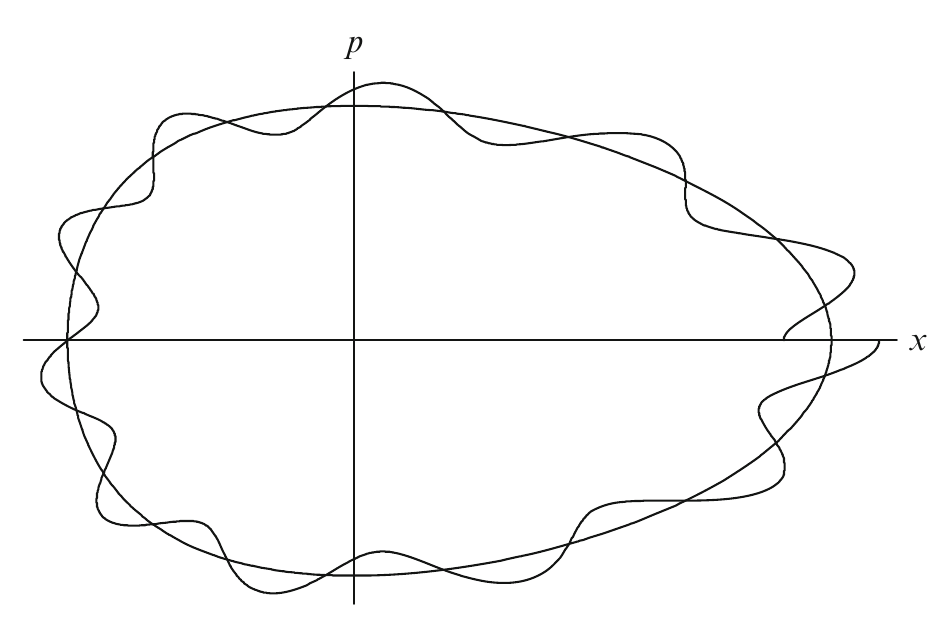
\includegraphics[width=0.76\textwidth]{figures/figure-15-1.png}
\caption{满足修正 Bohr--Sommerfeld 条件的轨道($n=10$).}
\label{fig:wkb-bohr-sommerfeld-trajectory}
\end{figure}

Bohr--Sommerfeld 条件要求沿曲线走一周后式~\eqref{eq:wkb-old-wave} 与自身衔接.这当且仅当
\[
\frac1\hbar\oint_Cp\,dx=2\pi n,
\qquad n\in\mathbb Z.
\label{eq:bohr-sommerfeld-old}
\]
旧量子理论把满足该条件的能量作为能级.Bohr--Sommerfeld 量子化曾取得一些成功,尤其是解释氢原子能级,但最终不能正确预测复杂系统的能量.

对一个自由度的系统,现代量子理论保留了这一方法的痕迹,但有两项修改.第一,把右端的 $n$ 改为 $n+1/2$,称为 Maslov 修正;第二,该条件通常只给出能级的主导阶半经典近似,而不是精确能级.

\begin{definition}[Maslov 修正的 Bohr--Sommerfeld 条件]\label{condition:maslov-bohr-sommerfeld}
若对某个非负整数 $n$,经典能量曲线 $C$ 满足
\[
\frac1\hbar\oint_Cp\,dx=2\pi\left(n+\frac12\right),
\label{eq:maslov-bohr-sommerfeld}
\]
则称能量 $E$ 满足 Maslov 修正的 Bohr--Sommerfeld 条件.由 Green 定理,这等价于
\[
\frac{\text{曲线 }C\text{ 所围面积}}{2\pi\hbar}=n+\frac12.
\]
\end{definition}

加入 Maslov 修正后,条件可以理解为:相位由式~\eqref{eq:wkb-old-wave} 的一形式积分给出的波,绕能量曲线一周后与自身相差 $180^\circ$.后面的分析将显示,额外的 $1/2$ 实际上来自两个转向点各贡献 $1/4$.在 WKB 近似中,波函数的相位是沿经典能量曲线的一条分支积分 $p\,dx/\hbar$;用 Airy 函数近似转向点附近的波函数,会在每个转向点与最后一个局部极大或极小之间产生额外的 $\pi/4$ 相位.由于能量曲线有两条分支,每个转向点的额外 $\pi/4$ 最终使左端积分增加 $\pi$.

氢原子的径向问题为何没有同样修正,可从有效势解释.氢原子的 Schrödinger 算子可化为一维 Schrödinger 算子,其有效势为
\[
V_{\mathrm{eff}}(r)=-\frac{Q^2}{r}+\frac{\hbar^2l(l+1)}{2mr^2},
\]
其中 $l$ 是标记总角动量的非负整数.径向波函数在 $r=0$ 必须满足零边界条件,这会额外引入 $1/2$ 修正;连同两个转向点各贡献 $1/4$,得到 $n+1$,于是形式上又回到未修正的 Bohr--Sommerfeld 条件.

\section{经典与半经典近似}
\label{sec:wkb-classical-semiclassical}

我们要研究小 $\hbar$ 下定态 Schrödinger 方程
\[
-\frac{\hbar^2}{2m}\frac{d^2\psi}{dx^2}+(V(x)-E)\psi(x)=0.
\label{eq:wkb-schrodinger}
\]
最终需要分析三个区域:经典允许区间($V(x)<E$)、经典禁阻区间($V(x)>E$)以及转向点附近($V(x)=E$).

先考虑经典允许区间.给定 $V$ 与能量 $E$,经典粒子的动量为
\[
p(x)=\sqrt{2m(E-V(x))}.
\]
寻找形如
\[
\psi(x)=A(x)e^{\pm iS(x)/\hbar},
\qquad S'(x)=p(x)
\label{eq:wkb-ansatz}
\]
的近似解.波函数的相位是 $\pm\hbar^{-1}\int p(x)\,dx$,振幅 $A(x)$ 取为与 $\hbar$ 无关的函数,相对于快速变化的 $S(x)/\hbar$ 而言是缓慢变化的.

\begin{proposition}[WKB 的初步近似特征向量]\label{prop:wkb-first-approximation}
设 $E_1>E_*:=\inf_{x\in\mathbb R}V(x)$.存在常数 $C$ 与非零函数 $A\in C_c^\infty(\mathbb R)$,使得对每个 $E\in[E_1,E_2]$,$A$ 的支集包含在能量 $E$ 的经典允许区间内,并且令
\[
\psi(x)=A(x)\exp\left(\pm\frac{i}{\hbar}\int p(x)\,dx\right)
\]
时,有
\[
\|\widehat H\psi-E\psi\|\leq C\hbar\|\psi\|.
\label{eq:wkb-first-error}
\]
\end{proposition}

\begin{proof}
能量 $E\in[E_1,E_2]$ 的经典允许区间包含能量 $E_1$ 的允许区间;取任意支集包含在后者中的非零 $A\in C_c^\infty$.直接计算 $\widehat H\psi-E\psi$,指数因子的两次微分产生 $p(x)^2$ 项,该项与 $V(x)-E$ 抵消,得到
\[
\widehat H\psi-E\psi
=-\left(\frac{\hbar^2}{2m}A''(x)\pm\frac{i\hbar}{2m}(2A'(x)p(x)+A(x)p'(x))\right)
\exp\left(\pm\frac{i}{\hbar}\int p(x)\,dx\right).
\label{eq:wkb-first-computation}
\]
因此
\[
\|\widehat H\psi-E\psi\|
\leq\frac{\hbar^2}{2m}\|A''\|+\frac{\hbar}{2m}\|2A'p+Ap'\|.
\]
$\|\psi\|$ 与 $\hbar$ 无关,且第二项在 $E\in[E_1,E_2]$ 上一致有界,故结论成立.
\end{proof}

由命题~\ref{prop:wkb-first-approximation} 与初等谱理论,任意大于 $\inf V$ 的 $E$ 都满足:谱中存在 $\widetilde E$,使 $|E-\widetilde E|\leq C\hbar$.若 $V(x)\to+\infty$($x\to\pm\infty$),则 $\widehat H$ 的谱离散,$\widetilde E$ 是特征值.因此当 $\hbar\to0$ 时,量子能谱在一定意义下填满经典能量函数的值域.不过这只能说明特征值间距至多为 $O(\hbar)$,并没有给出各个特征值的具体位置.

本章将证明:若 $E$ 满足 Maslov 修正的 Bohr--Sommerfeld 条件,则存在 $\widehat H$ 的特征值 $\widetilde E$,使
\[
|E-\widetilde E|\leq C\hbar^{9/8}.
\label{eq:wkb-main-error}
\]
这给出的误差小于预期的能级平均间距 $O(\hbar)$,因此是一个半经典估计:用经典能量曲线的位置估计量子能级.

\section{远离转向点的 WKB 近似}
\label{sec:wkb-away-turning-points}

\begin{definition}[WKB 分析的假设]\label{assumption:wkb}
设 $V$ 是光滑实值势函数,且 $V(x)\to+\infty$($x\to\pm\infty$).假设在无穷远附近,$V'(x)/V(x)$ 与 $V''(x)/V(x)$ 有界.给定能量范围 $E_1\leq E\leq E_2$,假设每个 $E$ 对应恰有两个转向点 $a(E)<b(E)$,满足 $V(a(E))=V(b(E))=E$,并且 $V'$ 在这些点处均非零.
\end{definition}

在此假设下,$\widehat H$ 在 $C_c^\infty(\mathbb R)$ 上本质自伴且具有纯离散谱.固定能量 $E$ 时,简写转向点为 $a,b$.

\begin{figure}[htbp]
\centering
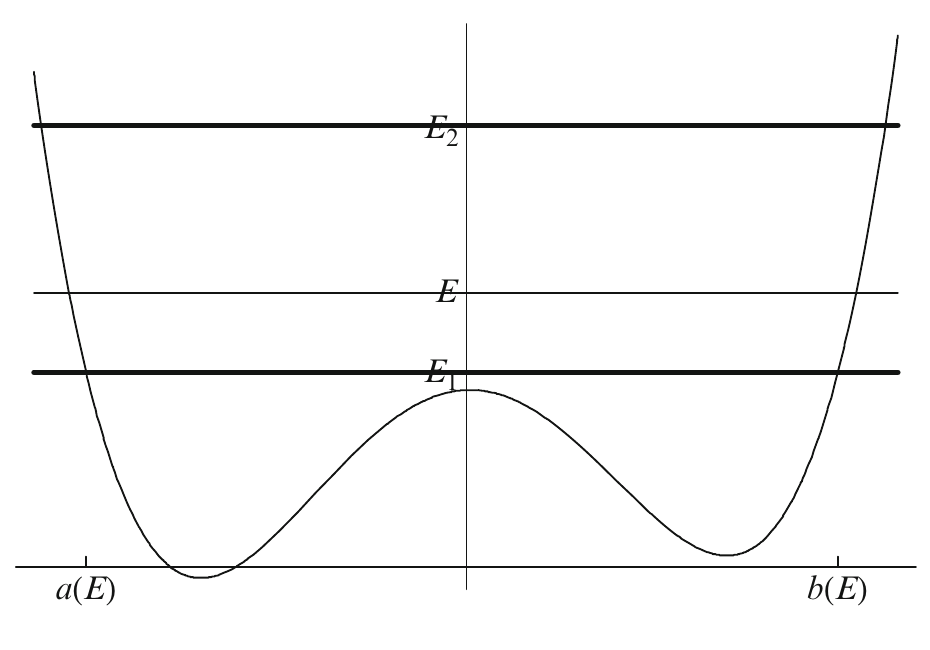
\includegraphics[width=0.76\textwidth]{figures/figure-15-2.png}
\caption{满足假设~\ref{assumption:wkb} 的一个势函数.}
\label{fig:wkb-potential-assumption}
\end{figure}

\subsection{经典允许区间}
\label{subsec:wkb-allowed}

仍取式~\eqref{eq:wkb-ansatz}.由式~\eqref{eq:wkb-first-computation},若希望误差小于 $O(\hbar)$,必须令 $A$ 满足
\[
2A'(x)p(x)=-p'(x)A(x),
\qquad
\frac{A'(x)}{A(x)}=-\frac12\frac{p'(x)}{p(x)}.
\label{eq:wkb-amplitude-ode}
\]
所以(见练习~\ref{ex:wkb-amplitude})
\[
A(x)=C p(x)^{-1/2}.
\label{eq:wkb-amplitude}
\]
此时
\[
\widehat H\psi-E\psi=-\frac{\hbar^2}{2m}\frac{A''(x)}{A(x)}\psi(x).
\label{eq:wkb-local-error}
\]
形式上误差为 $O(\hbar^2)$,但该式只在允许区间局部成立;$p(x)$ 在转向点趋于零,故振幅在转向点发散.

取两个相反指数的线性组合,并把积分基点取为左转向点 $a$.由于 Schrödinger 算子与复共轭对易,可以只考虑实值近似解.

\begin{note}[振荡型 WKB 函数]\label{note:wkb-oscillatory}
在经典允许区间且远离转向点处,实值 Schrödinger 解应近似为
\[
\psi(x)\approx\frac{R}{\sqrt{p(x)}}
\cos\left(\frac1\hbar\int_a^xp(y)\,dy-\delta\right),
\label{eq:wkb-oscillatory}
\]
其中 $R,\delta$ 是实常数,分别称为振幅与相位.
\end{note}

对式~\eqref{eq:wkb-oscillatory} 的平方使用 $\cos^2\theta=(1+\cos2\theta)/2$.小 $\hbar$ 时快速振荡的余弦项因正负抵消而较小,所以概率密度的主导项与 $1/p(x)$ 成正比,即与 $1/v(x)$ 成正比;而 $1/v(x)=dt/dx$,故粒子在某区间内出现的概率近似等于经典粒子在该区间内所用时间占一个周期的比例.

\subsection{经典禁阻区间}
\label{subsec:wkb-forbidden}

令
\[
q(x)=\sqrt{2m(V(x)-E)}.
\]
在经典禁阻区间寻找
\[
\psi(x)=A(x)\exp\left(\pm\frac1\hbar\int q(y)\,dy\right).
\]
同样分析可知,为抵消 $O(\hbar)$ 项,唯一的振幅(相差常数倍)为 $A(x)=Cq(x)^{-1/2}$.在 $(b,+\infty)$ 上,为得到平方可积解取负号并以 $b$ 为积分基点;在 $(-\infty,a)$ 上取正号并反向积分,最终也可写成负指数.

\begin{note}[指数型 WKB 函数]\label{note:wkb-exponential}
若 $\psi_1$ 是趋于 $-\infty$ 时趋于零的定态解,则在 $(-\infty,a)$ 且远离 $a$ 处,
\[
\psi_1(x)\approx\frac{c_1}{\sqrt{q(x)}}
\exp\left(-\frac1\hbar\int_x^a q(y)\,dy\right).
\label{eq:wkb-left-forbidden}
\]
若 $\psi_2$ 是趋于 $+\infty$ 时趋于零的定态解,则在 $(b,+\infty)$ 且远离 $b$ 处,
\[
\psi_2(x)\approx\frac{c_2}{\sqrt{q(x)}}
\exp\left(-\frac1\hbar\int_b^x q(y)\,dy\right).
\label{eq:wkb-right-forbidden}
\]
转向点处的奇异性只是近似方法的产物;真实的光滑势的定态解是光滑的,并且在小 $\hbar$ 下只会在非常靠近转向点时偏离 WKB 近似.
\end{note}

\begin{figure}[htbp]
\centering
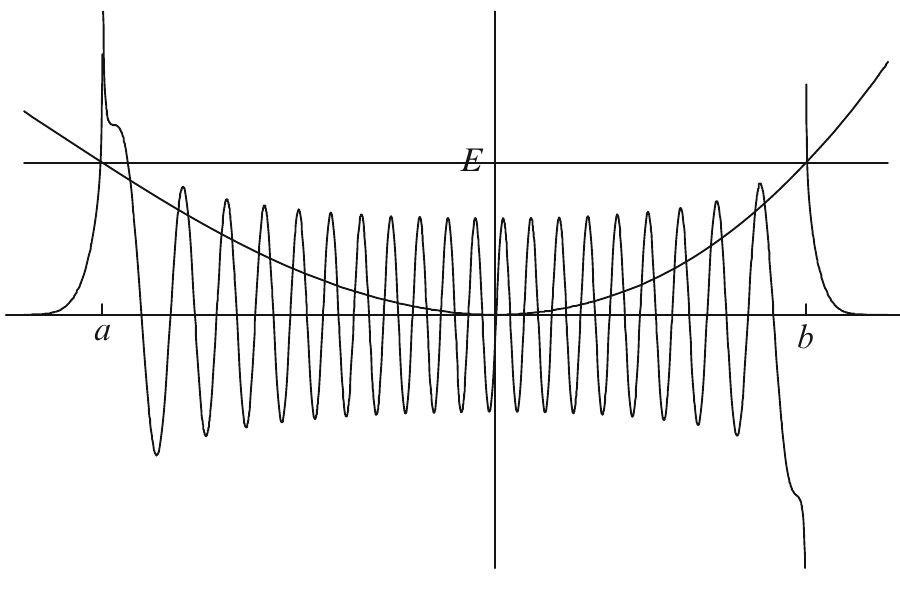
\includegraphics[width=0.76\textwidth]{figures/figure-15-3.png}
\caption{把 WKB 函数一直延拓到转向点.}
\label{fig:wkb-extended-functions}
\end{figure}

\section{Airy 函数与连接公式}
\label{sec:wkb-airy-connection}

若 $\psi_1$ 在 $-\infty$ 处衰减,则它在允许区间的振荡近似中的常数 $R,\delta$ 应当由左转向点附近的连接公式决定.设
\[
F_0=-V'(a)>0,
\qquad V(x)\approx(a-x)F_0.
\]
Schrödinger 方程在 $a$ 附近近似为
\[
-\frac{\hbar^2}{2m}\frac{d^2\psi}{dx^2}+(a-x)F_0\psi=0.
\]
作变量代换
\[
u=\left(\frac{2mF_0}{\hbar^2}\right)^{1/3}(a-x),
\label{eq:wkb-airy-variable}
\]
得到 Airy 方程
\[
\frac{d^2\psi}{du^2}-u\psi(u)=0.
\label{eq:airy-equation}
\]
它有两个线性无关解 $\operatorname{Ai}(u),\operatorname{Bi}(u)$;因为 $\operatorname{Ai}(u)$ 在 $u>0$(即 $x<a$)衰减,我们取
\[
\operatorname{Ai}(u)=\frac1\pi\int_0^\infty\cos\left(\frac{t^3}{3}+ut\right)\,dt.
\label{eq:airy-integral}
\]
积分由快速振荡收敛,严格证明可用练习~\ref{ex:airy-convergence} 的分部积分.对 $u$ 大小的渐近性可由驻相法与反复分部积分得到.

\begin{proposition}[Airy 连接公式]\label{claim:airy-connection}
若 $\psi_1$ 是在 $-\infty$ 附近趋于零的 Schrödinger 方程解,则可归一化使
\begin{align}
\psi_1(x)&\approx\frac1{2\sqrt{q(x)}}\exp\left(-\frac1\hbar\int_x^a q(y)\,dy\right), &&x\to-\infty,\\
\psi_1(x)&\approx\frac{\sqrt\pi}{(2mF_0\hbar)^{1/6}}
\operatorname{Ai}\left(\left(\frac{2mF_0}{\hbar^2}\right)^{1/3}(a-x)\right), &&x\approx a,\\
\psi_1(x)&\approx\frac1{\sqrt{p(x)}}\cos\left(\frac1\hbar\int_a^xp(y)\,dy-\frac\pi4\right), &&a<x<b.
\end{align}
\end{proposition}

类似地,若 $\psi_2$ 在 $+\infty$ 处趋于零,令 $F_1=V'(b)>0$,则
\begin{align}
\psi_2(x)&\approx\frac1{\sqrt{p(x)}}\cos\left(-\frac1\hbar\int_x^bp(y)\,dy+\frac\pi4\right), &&a<x<b,\\
\psi_2(x)&\approx\frac{\sqrt\pi}{(2mF_1\hbar)^{1/6}}
\operatorname{Ai}\left(\left(\frac{2mF_1}{\hbar^2}\right)^{1/3}(x-b)\right), &&x\approx b,\\
\psi_2(x)&\approx\frac1{2\sqrt{q(x)}}\exp\left(-\frac1\hbar\int_b^xq(y)\,dy\right), &&x\to+\infty.
\end{align}

\begin{figure}[htbp]
\centering
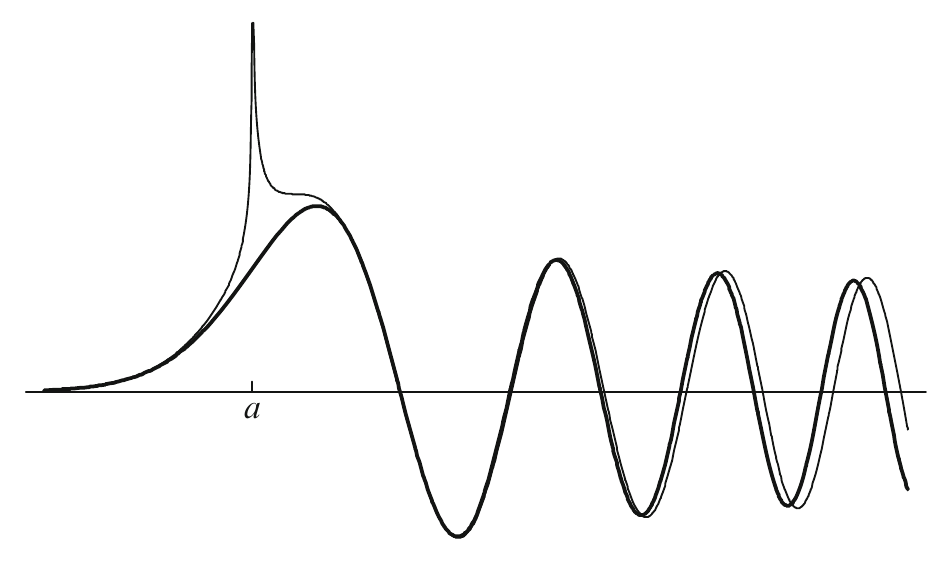
\includegraphics[width=0.76\textwidth]{figures/figure-15-4.png}
\caption{转向点 $x=a$ 附近缩放后的 Airy 函数(粗曲线)与 WKB 函数.}
\label{fig:wkb-airy-wkb-comparison}
\end{figure}

\begin{figure}[htbp]
\centering
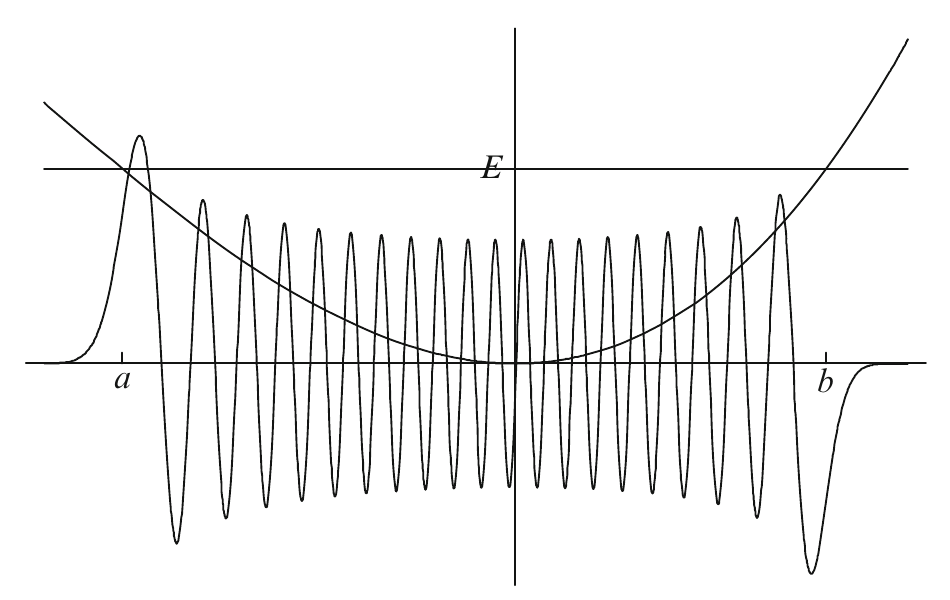
\includegraphics[width=0.76\textwidth]{figures/figure-15-5.png}
\caption{$n=39$ 时的近似波函数.}
\label{fig:wkb-approximate-wavefunction}
\end{figure}

\begin{figure}[htbp]
\centering
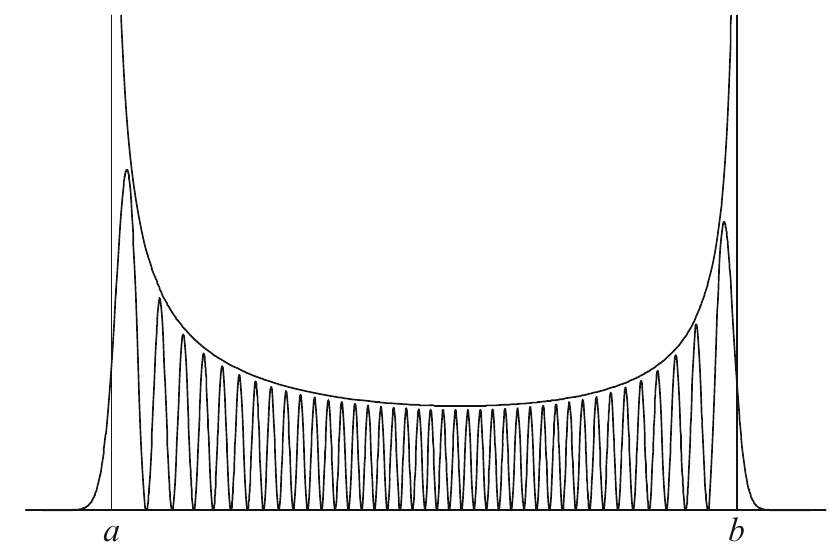
\includegraphics[width=0.76\textwidth]{figures/figure-15-6.png}
\caption{近似波函数的概率分布与函数 $1/p(x)$ 的比较.}
\label{fig:wkb-probability-distribution}
\end{figure}

Airy 函数的两条渐近公式为
\[
\operatorname{Ai}(u)\approx\frac1{2\sqrt\pi}u^{-1/4}e^{-2u^{3/2}/3},
\qquad u\to+\infty,
\label{eq:airy-positive-asymptotic}
\]
以及
\[
\operatorname{Ai}(u)\approx\frac1{\sqrt\pi(-u)^{1/4}}
\cos\left(\frac23(-u)^{3/2}-\frac\pi4\right),
\qquad u\to-\infty.
\label{eq:airy-negative-asymptotic}
\]
在左转向点附近的线性近似给出
\[
p(x)\approx\sqrt{2mF_0}\sqrt{x-a},
\qquad
\frac1\hbar\int_a^xp(y)\,dy\approx\frac23(-u)^{3/2}.
\]
代入式~\eqref{eq:airy-negative-asymptotic} 即得到左连接公式;式~\eqref{eq:airy-positive-asymptotic} 给出禁阻区间的指数型公式.右转向点同理.

\begin{proposition}[WKB 能量匹配条件]\label{prop:wkb-matching-condition}
左右两侧得到的允许区间近似解当且仅当存在非负整数 $n$,使
\[
\frac1\hbar\int_a^bp(x)\,dx=\left(n+\frac12\right)\pi.
\label{eq:wkb-matching}
\]
该条件等价于定义~\ref{condition:maslov-bohr-sommerfeld} 中的 Maslov 修正 Bohr--Sommerfeld 条件.若 $n$ 为偶数,左右近似解相等;若 $n$ 为奇数,它们互为相反数.
\end{proposition}

\begin{proof}
令
\[
\phi=\frac1\hbar\int_a^bp(y)\,dy-\frac\pi2.
\]
左侧相位与右侧相位相差 $\phi$.当 $\phi$ 为 $\pi$ 的偶数倍或奇数倍时,两个余弦分别相等或互为相反数;其他情形下,一个余弦函数不可能是另一个余弦函数的常数倍(见练习~\ref{ex:wkb-phase}).故式~\eqref{eq:wkb-matching} 是必要且充分的.
\end{proof}

\section{严格误差估计}
\label{sec:wkb-rigorous-error}

前面的各节给出了许多教材中常见的 WKB 近似处理.这样的处理说明:满足修正 Bohr--Sommerfeld 条件(条件~\ref{condition:maslov-bohr-sommerfeld})的能量应该是 Hamilton 算子 $\widehat H$ 的近似特征值,但还没有说明“近似”究竟具有什么严格含义.本节证明如下的估计.

\begin{theorem}[WKB 近似的严格误差估计]\label{thm:wkb-rigorous-error}
对满足假设~\ref{assumption:wkb} 的任意势函数 $V$ 与能量范围 $[E_1,E_2]$,存在常数 $C$,使得:对 $[E_1,E_2]$ 中满足条件~\ref{condition:maslov-bohr-sommerfeld} 的任意能量 $E$,都存在非零函数 $\psi\in\operatorname{Dom}(\widehat H)$,满足
\[
\|\widehat H\psi-E\psi\|<C\hbar^{9/8}\|\psi\|.
\label{eq:wkb-rigorous-residual}
\]
\end{theorem}

如第~\ref{sec:wkb-classical-semiclassical} 节已经指出,若存在满足
$\|\widehat H\psi-E\psi\|<\varepsilon\|\psi\|$ 的函数,则 $\widehat H$ 的谱中存在某个 $\widetilde E$,使 $|E-\widetilde E|<\varepsilon$(见第 10 章练习 4).由于在假设~\ref{assumption:wkb} 下 $\widehat H$ 的谱纯离散,我们得到:对于每个满足条件~\ref{condition:maslov-bohr-sommerfeld} 的 $E\in[E_1,E_2]$,$\widehat H$ 都有一个真正的特征值 $\widetilde E$,满足
\[
|E-\widetilde E|<C\hbar^{9/8}.
\label{eq:wkb-eigenvalue-error}
\]

如果 $E$ 满足条件~\ref{condition:maslov-bohr-sommerfeld},实际上可以证明式~\eqref{eq:wkb-eigenvalue-error} 右侧的 $\hbar^{9/8}$ 可替换为 $\hbar^2$.不过,用本章的方法不可能得到这样的最优估计:本定理证明中构造的近似特征向量并不满足 $\|\widehat H\psi-E\psi\|<C\hbar^2\|\psi\|$.另一方面,可以用其他方法(例如参考文献~[31] 中的方法)构造出误差为 $O(\hbar^2)$ 的近似特征向量.尽管如此,式~\eqref{eq:wkb-eigenvalue-error} 中的误差相对于能级的典型间距仍然很小,因为后者的数量级为 $\hbar$.

回忆假设~\ref{assumption:wkb}:势函数光滑并且在两端趋于 $+\infty$ 的 Schrödinger 算子在 $C_c^\infty(\mathbb R)$ 上本质自伴.本定理中的 $\widehat H$ 更准确地说,是定义在 $C_c^\infty(\mathbb R)$ 上的 Schrödinger 算子的唯一自伴延拓.

\subsection{准备工作}
\label{subsec:wkb-rigorous-preliminaries}

近似特征函数 $\psi$ 的构造基本按照命题~\ref{claim:airy-connection} 中概述的 WKB 近似进行:在转向点附近使用缩放后的 Airy 函数,在经典允许区间和禁阻区间使用标准 WKB 函数.不过,这种做法存在一个困难:缩放后的 Airy 函数在不同区域的边界处并不与 WKB 函数完全相同,而只是近似相同.于是,如果在形如 $(-\infty,a-\varepsilon)$ 的区间上用 WKB 公式定义 $\psi$,在 $(a-\varepsilon,a+\varepsilon)$ 上用缩放后的 Airy 函数定义 $\psi$,那么 $\psi$ 在 $a-\varepsilon$ 处可能不连续.即使在某个区间上乘以常数消除了 $\psi$ 本身的不连续,其导数通常仍会不连续.但如果 $\psi'$ 不连续,$\psi$ 就不属于 $\widehat H$ 的定义域,式~\eqref{eq:wkb-rigorous-residual} 的左端也就没有意义(可与第 5 章相应讨论比较).

要求 $\psi'$ 连续并不只是技术细节.如果不关心导数的连续性,就可以无论能量是否满足修正 Bohr--Sommerfeld 条件,都通过分别乘以常数把缩放后的 Airy 函数与 WKB 函数接起来.那样就会错误地声称 $[E_1,E_2]$ 中的任意 $E$ 都距 $\widehat H$ 的某个特征值至多 $C\hbar^{9/8}$;对谐振子而言这显然是错误的.

为克服上述困难,必须加入过渡区,在其中用光滑方式从一个函数过渡到另一个函数;这就是小节~\ref{subsec:wkb-transition-regions} 中的“拼接”构造.具体地说,在命题~\ref{claim:airy-connection} 所列的区间内使用相应公式,并在 $n$ 为奇数时把相应的允许区间函数及右侧匹配函数乘以 $-1$.在 $(a-\varepsilon,a+\varepsilon)$ 和 $(b-\varepsilon,b+\varepsilon)$ 上分别使用缩放后的 Airy 函数,再加入四个长度为 $\delta$ 的过渡区;$\varepsilon,\delta$ 随 $\hbar$ 的具体选择将在下面给出.图~\ref{fig:wkb-approximate-eigenfunction} 示意了转向点 $x=a$ 附近的过渡区.

\begin{figure}[htbp]
\centering
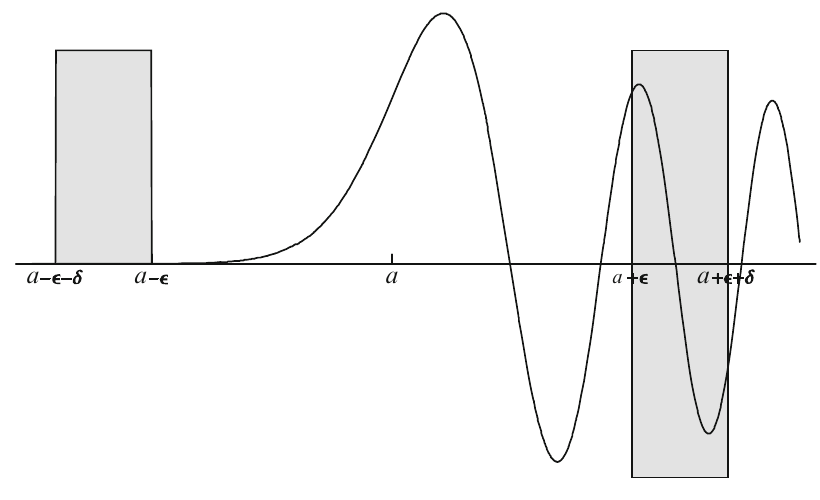
\includegraphics[width=0.78\textwidth]{figures/figure-15-7.png}
\caption{带有阴影过渡区的近似特征函数 $\psi$.}
\label{fig:wkb-approximate-eigenfunction}
\end{figure}

设 $\widehat H_0$ 是势函数为 $V$、定义域为 $C_c^\infty(\mathbb R)$ 的 Schrödinger 算子.由前面的讨论,$\widehat H_0$ 本质自伴;令 $\widehat H$(与伴随算子 $\widehat H_0^*$ 一致)表示它的唯一自伴延拓.$\widehat H_0^*$ 的定义域由所有满足以下条件的 $\psi\in L^2(\mathbb R)$ 组成:以分布意义计算的 Schrödinger 算子作用于 $\psi$ 后仍属于 $L^2(\mathbb R)$.特别地,如果 $\psi$ 光滑,则 $\psi\in\operatorname{Dom}(\widehat H)=\operatorname{Dom}(\widehat H_0^*)$ 当且仅当 $\psi\in L^2(\mathbb R)$ 且
\[
-\frac{\hbar^2}{2m}\psi''+V\psi\in L^2(\mathbb R).
\label{eq:wkb-domain-criterion}
\]

由于使用了拼接,构造出的近似特征函数 $\psi$ 在整个 $\mathbb R$ 上实际上是无穷可微的.又因为 $V(x)$ 在两端趋于 $+\infty$,指数型 WKB 函数在无穷远处快速衰减,所以 $\psi\in L^2(\mathbb R)$.在 $x$ 接近两端无穷远处,前面的计算(式~\eqref{eq:wkb-local-error})适用;取 $A(x)=Cq(x)^{-1/2}$,直接计算得到
\[
-\frac{\hbar^2}{2m}\psi''(x)+V(x)\psi(x)
=-\frac{\hbar^2}{2m}\left[
\frac5{16}\left(\frac{V'(x)}{V(x)-E}\right)^2
-\frac14\frac{V''(x)}{V(x)-E}
\right]\psi(x).
\label{eq:wkb-domain-error}
\]
由于假设 $V'/V$ 与 $V''/V$ 在无穷远处有界,且 $V(x)\to+\infty$,上式说明在无穷远处 Schrödinger 算子作用于 $\psi$ 的结果被 $\psi$ 的常数倍控制,因而属于平方可积函数.这证明了 $\psi\in\operatorname{Dom}(\widehat H)$.

在小节~\ref{subsec:wkb-turning-point-regions} 中,我们将取转向点附近区间的宽度 $2\varepsilon$ 为 $O(\hbar^{1/2})$.尽管 Airy 函数在非常靠近转向点处有 $O(\hbar^{-1/6})$ 的发散,近似波函数的 $L^2$ 范数在 $\hbar\to0$ 时仍为 $O(1)$(有正的下界且有有限上界).这不难验证(见练习~\ref{ex:wkb-norm});即便范数发散,也只会使证明 $\|\widehat H\psi-E\psi\|$ 相对于 $\|\psi\|$ 很小变得更容易.

为了证明定理~\ref{thm:wkb-rigorous-error},必须分别估计四类区域对 $\|\widehat H\psi-E\psi\|$ 的贡献:经典允许区间、经典禁阻区间、转向点附近的区域以及过渡区.下面各小节将完成这些估计,其中过渡区的分析最为复杂.特别重要的是,在过渡区内缩放后的 Airy 函数的导数必须几乎与 WKB 函数的导数匹配,这正是引理~\ref{lem:wkb-transition-mismatch} 的第二部分.

\subsection{转向点附近的区域}
\label{subsec:wkb-turning-point-regions}

在每个转向点附近的区间内使用缩放后的 Airy 函数(在 $x=a$ 附近使用式~\eqref{eq:wkb-airy-variable} 所对应的函数,在 $x=b$ 附近则根据 $n$ 的奇偶性使用相应函数或其相反数).下面验证,取这些区间的长度为 $O(\hbar^{1/2})$ 会得到足够好的估计.

若 $\psi$ 是其中一个缩放后的 Airy 函数,则它满足一个把势函数 $V$ 换成转向点附近线性近似 $\widetilde V$ 的 Schrödinger 方程.因此
\[
\widehat H\psi-E\psi=(V(x)-\widetilde V(x))\psi.
\label{eq:wkb-turning-residual}
\]
势函数 $V$ 与线性近似 $\widetilde V$ 的差至多按距转向点的距离的平方增长.另一方面,Airy 函数的渐近式给出 $|\operatorname{Ai}(u)|\leq Cu^{-1/4}$(对小 $u$ 来说这是很差的估计,但仍然成立).式~\eqref{eq:wkb-airy-variable} 中的 $u$ 的数量级为 $\hbar^{-2/3}$ 乘以距转向点的距离;式中的缩放因子还有 $\hbar^{-1/6}$,而距转向点至多为 $O(\hbar^{1/2})$.因此,在转向点附近区间上
\[
|\widehat H\psi-E\psi|
\leq C(\hbar^{1/2})^2\hbar^{-1/6}
\bigl(\hbar^{-2/3}\hbar^{1/2}\bigr)^{-1/4}
=C\hbar^{7/8}.
\]
若函数 $f$ 在长度为 $L$ 的区间上满足 $|f|\leq D$,则其在该区间上的 $L^2$ 范数至多为 $D\sqrt L$.所以转向点附近区域的贡献为
\[
\|\widehat H\psi-E\psi\|=O(\hbar^{7/8}\hbar^{1/4})=O(\hbar^{9/8}).
\label{eq:wkb-turning-error}
\]

\subsection{经典允许区间与经典禁阻区间}
\label{subsec:wkb-allowed-forbidden-error}

由式~\eqref{eq:wkb-domain-error}(它由式~\eqref{eq:wkb-local-error} 得到)给出的表达式,在经典允许区间和禁阻区间都适用.先考虑经典允许区间.虽然式~\eqref{eq:wkb-domain-error} 形式上是 $O(\hbar^2)$,但我们是在端点随 $\hbar\to0$ 逐渐靠近转向点的区间上使用它;而且式中的表达式在转向点处发散,所以这一段对 $\|\widehat H\psi-E\psi\|$ 的贡献会大于 $\hbar^2$ 的数量级.

转向点附近区间的宽度 $2\varepsilon$ 取为 $O(\hbar^{1/2})$,并且下面还会取过渡区宽度 $\delta=O(\hbar^{1/2})$.因此,在经典允许区间中使用振荡型 WKB 函数的区间可写成 $(a+\gamma,b-\gamma)$,其中 $\gamma=\varepsilon+\delta=O(\hbar^{1/2})$.

允许区间中的 $\psi$ 含有 $p(x)^{-1/2}$ 因子和有界的余弦因子.由于 $V'(a)\neq0$,当 $x\to a$ 时,$V(x)-E$ 的行为与 $x-a$ 成正比,从而 $p(x)^{-1/2}$ 与 $(x-a)^{-1/4}$ 成正比;在另一个转向点附近也有类似行为.另一方面,式~\eqref{eq:wkb-domain-error} 中问题最大的项含有 $(V(x)-E)^{-2}$,再考虑 $\psi$ 自身的 $p(x)^{-1/2}$ 发散,该项在 $a$ 附近的行为为 $(x-a)^{-9/4}$.于是,在允许区间左半段可估计为
\[
\begin{aligned}
\|\widehat H\psi-E\psi\|&\leq C\hbar^2
\left(\int_{a+\gamma}^{(a+b)/2}(x-a)^{-9/2}\,dx\right)^{1/2}\\
&=C'\hbar^2\left(\gamma^{-7/2}-\left(\frac{a+b}{2}-a\right)^{-7/2}\right)^{1/2}.
\end{aligned}
\]
由于 $\gamma=O(\hbar^{1/2})$,该贡献的主导项为 $\hbar^2\hbar^{-7/8}=\hbar^{9/8}$;允许区间的另一半同理.

在第一个经典禁阻区间中也使用式~\eqref{eq:wkb-domain-error}.由假设~\ref{assumption:wkb},$V'/V$ 与 $V''/V$ 在无穷远处有界;因此 $V'/(V-E)$ 与 $V''/(V-E)$ 在无穷远处也有界,并且在 $(-\infty,a-1)$ 上有界,因为 $V-E$ 在该区间严格为正且在 $x\to-\infty$ 时趋于 $+\infty$.所以该区间上 $\|\widehat H\psi-E\psi\|$ 至多为常数乘以 $\hbar^2\|\psi\|$.在 $(a-1,a-\gamma)$ 上的估计与允许区间相似,但此处还有 WKB 函数的指数衰减因子,因此经典禁阻区间 $(-\infty,a-\gamma)$ 的贡献肯定不超过 $O(\hbar^{9/8})$;右侧禁阻区间同理.

\subsection{过渡区}
\label{subsec:wkb-transition-regions}

给定两个光滑函数 $\psi_1,\psi_2$ 以及形如 $[\alpha,\alpha+\delta]$ 的区间,定义它们的“拼接” $\psi_1;\psi_2$:当 $x<\alpha$ 时等于 $\psi_1(x)$,当 $x>\alpha+\delta$ 时等于 $\psi_2(x)$,并且在整个实轴上光滑.取 $[0,1]$ 上的光滑函数 $\chi$,使其在 $0$ 的某邻域恒为 $0$、在 $1$ 的某邻域恒为 $1$.定义
\[
(\psi_1;\psi_2)(x)=\psi_1(x)+(\psi_2(x)-\psi_1(x))\chi\left(\frac{x-\alpha}{\delta}\right).
\label{eq:wkb-join}
\]

图~\ref{fig:wkb-join} 给出了示意图.直接计算得到
\[
\begin{aligned}
(\widehat H-EI)(\psi_1;\psi_2)
={}&(\widehat H\psi_1-E\psi_1);(\widehat H\psi_2-E\psi_2)\\
&-\frac{\hbar^2}{m\delta}(\psi_2'(x)-\psi_1'(x))\chi'\left(\frac{x-\alpha}{\delta}\right)\\
&-\frac{\hbar^2}{2m\delta^2}(\psi_2(x)-\psi_1(x))\chi''\left(\frac{x-\alpha}{\delta}\right).
\end{aligned}
\label{eq:wkb-join-error}
\]

\begin{figure}[htbp]
\centering
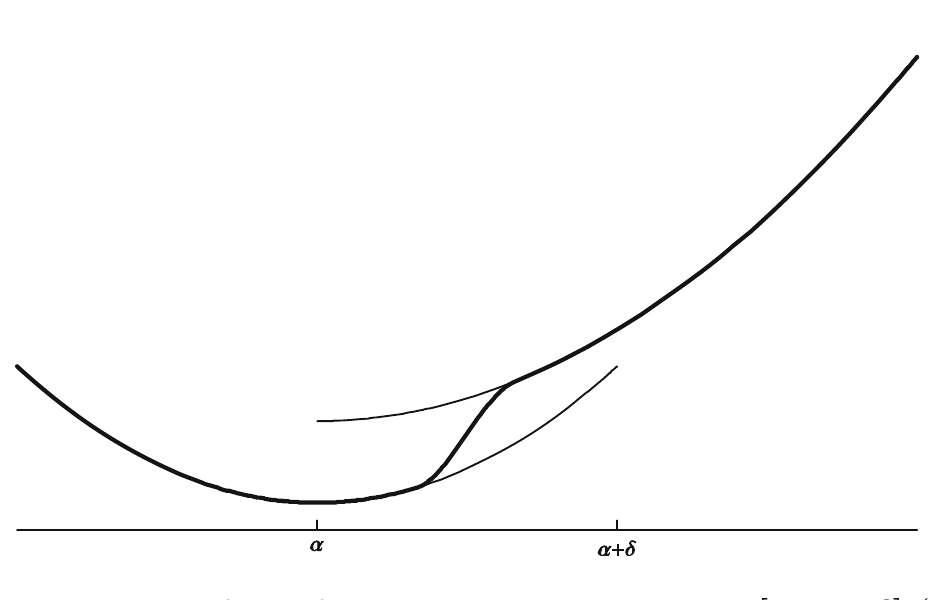
\includegraphics[width=0.78\textwidth]{figures/figure-15-8.png}
\caption{在区间 $[\alpha,\alpha+\delta]$ 上拼接两个函数;粗曲线表示拼接函数.}
\label{fig:wkb-join}
\end{figure}

我们在五个不同区域使用五种不同公式:两个经典禁阻区间、一个经典允许区间以及两个转向点附近的区域.由于相邻区间中的函数并不完全匹配,必须使用四次拼接,才能得到属于 $\widehat H$ 定义域的函数.拼接区间的宽度 $\delta$ 取为与转向点附近区间相同的数量级,即 $O(\hbar^{1/2})$.

最关键的情况是从转向点附近区域过渡到经典允许区间.以左转向点为例,令 $\psi_1$ 为式~\eqref{eq:wkb-airy-variable} 对应的缩放 Airy 函数,令 $\psi_2$ 为振荡型 WKB 函数.二者的不匹配有两个来源:第一,Airy 函数与其主导渐近式之间存在差异;第二,式~\eqref{eq:airy-negative-asymptotic} 与连接公式中所用的近似,忽略了势函数 $V$ 与其在 $x=a$ 处的线性近似 $\widetilde V$ 之间的差异.估计 $\psi_1-\psi_2$ 及其导数时,必须同时考虑这两项.

\begin{lemma}[过渡区中的 Airy--WKB 匹配]\label{lem:wkb-transition-mismatch}
令 $\psi_1$ 是左转向点处的缩放 Airy 函数,令 $\widetilde\psi_1$ 是把其中的 Airy 函数替换为式~\eqref{eq:airy-negative-asymptotic} 右端所得的函数,令 $\psi_2$ 是振荡型 WKB 函数.当 $x-a$ 为 $O(\hbar^{1/2})$ 时,有
\[
|\psi_1(x)-\widetilde\psi_1(x)|=O(\hbar^{1/8}),
\qquad
|\widetilde\psi_1(x)-\psi_2(x)|=O(\hbar^{1/8}),
\label{eq:wkb-function-mismatch}
\]
且
\[
|\psi_1'(x)-\widetilde\psi_1'(x)|=O(\hbar^{-5/8}),
\qquad
|\widetilde\psi_1'(x)-\psi_2'(x)|=O(\hbar^{-5/8}).
\label{eq:wkb-derivative-mismatch}
\]
\end{lemma}

先说明这个引理的估计足以控制转向点附近区域 $(a+\varepsilon,a+\varepsilon+\delta)$ 对误差的贡献,其中 $\varepsilon,\delta=O(\hbar^{1/2})$.拼接误差式~\eqref{eq:wkb-join-error} 的第一行的 $L^2$ 范数至多为 $O(\hbar^{9/8})$,理由与小节~\ref{subsec:wkb-allowed-forbidden-error} 中相同.若函数在长度为 $L$ 的区间上绝对值不超过 $C$,则其 $L^2$ 范数至多为 $C\sqrt L$.因此,第二行的 $L^2$ 范数为
\[
O\left(\delta^{-1}\hbar^2\hbar^{-5/8}\delta^{1/2}\right)
=O(\hbar^{9/8}),
\]
而第三行的贡献为
\[
O\left(\delta^{-2}\hbar^2\hbar^{1/8}\delta^{1/2}\right)
=O(\hbar^{11/8}).
\]
所以该过渡区的总贡献至多为 $O(\hbar^{9/8})$.从经典允许区间过渡到右转向点附近区域的分析完全相同.转向点附近区域与经典禁阻区间之间的过渡则容易得多,因为参与拼接的所有函数在过渡区内都很小.例如,当 $a-x=O(\hbar^{1/2})$ 时,Airy 变量 $u$ 为 $O(\hbar^{-1/6})$,因而 $u^{3/2}=O(\hbar^{-1/4})$;$u>0$ 时 Airy 函数渐近式中的指数因子形如 $\exp(-C\hbar^{-1/4})$,对小 $\hbar$ 而言比任意幂次的 $\hbar$ 都小.因此这些过渡区的贡献小于任意给定的 $\hbar$ 幂次,当然不会超过 $O(\hbar^{9/8})$.

\begin{proof}
我们只证明引理中关于导数的估计;关于函数本身的估计类似而且更容易,留给练习~\ref{ex:wkb-mismatch-functions}.

先考虑 $\psi_1'-\widetilde\psi_1'$.直接计算得到
\[
\psi_1'(x)-\widetilde\psi_1'(x)
=-\sqrt\pi(2mF_0)^{1/6}\hbar^{-5/6}
\left(\operatorname{Ai}'(u)-\widetilde{\operatorname{Ai}}'(u)\right),
\label{eq:wkb-airy-derivative-difference}
\]
其中 $u$ 如式~\eqref{eq:wkb-airy-variable},$\widetilde{\operatorname{Ai}}$ 表示式~\eqref{eq:airy-negative-asymptotic} 右端的函数.

当 $u\to-\infty$ 时,$\operatorname{Ai}(u)$ 有渐近展开
\[
\widetilde{\operatorname{Ai}}(u)=\operatorname{Ai}(u)\bigl(1+O((-u)^{-3/2})\bigr),
\]
而 $\operatorname{Ai}'(u)$ 的展开可由对上式关于 $u$ 形式求导得到.因此
\[
\operatorname{Ai}'(u)-\widetilde{\operatorname{Ai}}'(u)
=\widetilde{\operatorname{Ai}}'(u)O((-u)^{-3/2})
+\widetilde{\operatorname{Ai}}(u)O((-u)^{-5/2}).
\label{eq:wkb-airy-asymptotic-error}
\]
从显式公式看,$\widetilde{\operatorname{Ai}}(u)$ 的数量级为 $(-u)^{-1/4}$,而 $\widetilde{\operatorname{Ai}}'(u)$ 含有一个数量级为 $(-u)^{1/4}$ 的主导项.所以式~\eqref{eq:wkb-airy-asymptotic-error} 右端衰减较慢的项为 $O((-u)^{-5/4})$.在过渡区,$u=O(\hbar^{-2/3}\hbar^{1/2})=O(\hbar^{-1/6})$,故式~\eqref{eq:wkb-airy-derivative-difference} 的数量级为
\[
\hbar^{-5/6}\hbar^{5/24}=\hbar^{-5/8},
\]
得到所需估计.

再考虑 $\widetilde\psi_1'-\psi_2'$.直接计算可知,$\widetilde\psi_1'$ 和 $\psi_2'$ 都由两项组成:对余弦因子求导得到的“主导项”,以及对余弦前系数求导得到的“次主导项”.在 $\widetilde\psi_1'$ 中,主导项可化为
\[
-\frac1\hbar\bigl((2mF_0)(x-a)\bigr)^{1/4}
\sin\left(\frac23(-u)^{3/2}-\frac\pi4\right).
\label{eq:wkb-airy-dominant-derivative}
\]
练习~\ref{ex:wkb-phase-expansion} 将证明,当 $x-a=O(\hbar^{1/2})$ 时
\[
\bigl((2mF_0)(x-a)\bigr)^{1/4}=\sqrt{p(x)}\bigl(1+O(\hbar^{1/2})\bigr),
\label{eq:wkb-amplitude-comparison}
\]
以及
\[
\frac23(-u)^{3/2}=\frac1\hbar\int_a^xp(y)\,dy+O(\hbar^{1/4}).
\label{eq:wkb-phase-comparison}
\]
由于 $\sin\theta$ 的导数有界,正弦函数自变量改变 $O(\hbar^{1/4})$ 时,函数值也只改变 $O(\hbar^{1/4})$.把式~\eqref{eq:wkb-amplitude-comparison} 与式~\eqref{eq:wkb-phase-comparison} 代入式~\eqref{eq:wkb-airy-dominant-derivative},两主导项的差为
\[
\frac1\hbar\sqrt{p(x)}O(\hbar^{1/4})+\text{更低阶项}.
\]
由于 $\sqrt{p(x)}$ 的数量级为 $(x-a)^{1/4}$,在过渡区为 $O(\hbar^{1/8})$,故误差为 $O(\hbar^{-5/8})$.最后,$\widetilde\psi_1'$ 和 $\psi_2'$ 中的次主导项分别容易看出也都是 $O(\hbar^{-5/8})$,所以即使不利用它们之间的抵消,也不改变估计的数量级.
\end{proof}

\subsection{主定理的证明}
\label{subsec:wkb-main-theorem-proof}

上面已经分别估计了经典允许区间和禁阻区间、转向点附近区域以及过渡区对 $\|\widehat H\psi-E\psi\|$ 的贡献;每一项都至多为 $O(\hbar^{9/8}\|\psi\|)$.因此只需验证这些估计中的常数在能量范围 $E_1\leq E\leq E_2$ 上一致有界.

这一点是直接的.例如在左转向点 $a$ 附近,由 Taylor 余项公式,$V(x)$ 与线性近似 $\widetilde V(x)$ 的差满足
\[
|V(x)-\widetilde V(x)|\leq\frac12 C|x-a|^2,
\]
其中 $C$ 是从 $a$ 到 $x$ 的区间上 $|V''|$ 的最大值.当 $E$ 在 $[E_1,E_2]$ 中变化时,需要考察 $V''$ 的点集是有界的,故 $C$ 可以取为与 $E$ 无关的常数.

类似地,在经典允许区间中,$1/(V(x)-E)^2$ 在 $x=a(E)$ 附近的发散可以用 $a(E)$ 与 $x$ 之间区间上 $|V'|$ 的最小值控制.由假设,在 $E_1\leq E\leq E_2$ 时所有转向点 $a(E),b(E)$ 处都有 $|V'|>0$;再由连续性,在这些转向点集合的某个邻域内仍有统一的正下界.因此,可取足够小的 $\alpha>0$,使得相关最小值由区间 $[a(E_2)+\alpha,a(E_1)+\alpha]$ 上 $|V'|$ 的最小值控制.其余细节留给读者.

\section{其他方法}
\label{sec:wkb-other-approaches}

WKB 近似的主要复杂性来自转向点附近的奇异行为.然而,转向点之所以造成困难,是因为我们在位置表象中工作.毕竟,转向点只是经典轨道上粒子位置达到最大值或最小值的点;如果改在动量表象中工作,那么动量达到最大值或最小值的点反而会成为问题点.A.~Voros 提议在 Segal--Bargmann 表象(见第~\ref{sec:segal-bargmann} 节)中工作.在 Voros 的分析中不存在转向点,因此分析大为简单.

Voros 方法的问题在于,它只在经典能量曲线上给出波函数的近似.即使在简单情形下,Voros 的表达式也不能全平面延拓为全纯函数,而是在经典能量曲线内部出现分支行为.因此,Voros 公式并不定义量子 Hilbert 空间中的元素(该空间由整函数组成),更不必说定义 Hamilton 算子定义域中的元素了.

尽管如此,仍然可以用相干态的叠加构造近似特征函数,所用公式与 Voros 的公式相似.这种方法避免了处理转向点,同时仍可得到严格的特征值估计,并且使用与条件~\ref{condition:maslov-bohr-sommerfeld} 相同的修正 Bohr--Sommerfeld 条件.见参考文献~[31,23,7];更一般的结果见参考文献~[26].

\section{习题}
\label{sec:wkb-exercises}

\begin{exercise}[复指数的余弦表示]\label{ex:wkb-cosine-combination}
证明:对任意复数 $c_1$,都存在实数 $R,\delta$,使
\[
c_1e^{i\theta}+\overline{c_1}e^{-i\theta}=R\cos(\theta-\delta).
\]
\end{exercise}

\begin{exercise}[谐振子的修正 Bohr--Sommerfeld 条件]\label{ex:wkb-harmonic-bohr-sommerfeld}
设
\[
H(x,p)=\frac{p^2}{2m}+\frac{m\omega^2x^2}{2}
\]
是质量为 $m$、经典频率为 $\omega$ 的谐振子 Hamilton 函数.证明:正数 $E$ 满足修正 Bohr--Sommerfeld 条件~\ref{condition:maslov-bohr-sommerfeld},当且仅当
\[
E=\left(n+\frac12\right)\hbar\omega,
\qquad n\in\mathbb Z_{\geq0}.
\]
\begin{note}[说明]\label{note:wkb-harmonic-exact}
结合第 11 章的结果,这个计算说明,在这个特殊情形中,修正 Bohr--Sommerfeld 条件给出了量子 Hamilton 算子的精确特征值.
\end{note}
\end{exercise}

\begin{exercise}[WKB 振幅方程]\label{ex:wkb-amplitude}
设 $A$ 与 $p$ 是满足式~\eqref{eq:wkb-amplitude-ode} 的两个非零光滑函数.证明存在常数 $C$,使 $A(x)=C p(x)^{-1/2}$.提示:考虑这些函数的对数.
\end{exercise}

\begin{exercise}[余弦相位的唯一性]\label{ex:wkb-phase}
证明:把 $\cos(\theta-\delta)$ 看作 $\theta$ 的函数,它与 $\cos(\theta-\delta')$ 相差一个常数倍,当且仅当 $\delta-\delta'$ 是 $\pi$ 的整数倍.
\end{exercise}

\begin{exercise}[解析延拓的振幅误差]\label{ex:wkb-analytic-continuation}
若 $\psi$ 是 $\widehat H$ 的特征向量,并且在 $-\infty$ 附近由式~\eqref{eq:wkb-left-forbidden} 近似,可以设想在复平面中绕过转向点作解析延拓,从而猜测经典允许区间中的近似表达式.即使 $V$ 是解析的,在上半平面和下半平面作解析延拓也显然不会给出相同答案;但可以把二者的平均作为一个完全非严格的猜测.证明:上述方法给出连接公式中的正确相位 $\delta$,但振幅 $R$ 差一个因子 $2$.
\end{exercise}

\begin{exercise}[Airy 积分的收敛性]\label{ex:airy-convergence}
用分部积分证明极限
\[
\lim_{A\to+\infty}\int_0^A\cos\left(\frac{t^3}{3}+ut\right)\,dt
\]
存在.提示:乘上并除以 $t^2+u$;当 $u<0$ 时避开 $t^2+u=0$ 的点.
\end{exercise}

\begin{exercise}[验证 Airy 方程]\label{ex:airy-equation-verification}
设 Airy 函数由式~\eqref{eq:airy-integral} 给出.假定可以在积分号下微分,验证它满足微分方程
\[
\operatorname{Ai}''(u)-u\operatorname{Ai}(u)=0.
\]
提示:在积分号下微分后,寻找一个可以显式积分的项.更严格的证明可以像练习~\ref{ex:airy-convergence} 那样先分部积分再在积分号下微分,但过程略显繁琐.
\end{exercise}

\begin{exercise}[Airy 函数的快速衰减]\label{ex:airy-rapid-decay}
在式~\eqref{eq:airy-integral} 中反复分部积分,证明当 $u\to+\infty$ 时,$\operatorname{Ai}(u)$ 比 $u$ 的任意负幂都衰减得更快.关键是证明每一步分部积分产生的边界项都为零;积分完成后,可使用
\[
\frac1{(t^2+u)^n}<\frac1{(t^2+1)^k u^{n-k}},\qquad u>1,
\]
其中 $k$ 适当选取.
\end{exercise}

\begin{exercise}[驻相法与 Airy 渐近式]\label{ex:airy-stationary-phase}
\begin{enumerate}
\item 当 $u<0$ 时,在 Airy 函数的积分公式中作变量代换 $\tau=t/\sqrt{-u}$,得到
\[
\operatorname{Ai}(u)=\frac{\sqrt{-u}}\pi\int_0^\infty\cos\left(\alpha\left(\frac{\tau^3}{3}-\tau\right)\right)\,d\tau,
\qquad \alpha=(-u)^{3/2}.
\]
\item 设 $f$ 是 $[a,b]$ 上的光滑函数,有唯一临界点 $x_0$,且 $x_0$ 在内部并满足 $f''(x_0)\neq0$.驻相法断言,当 $\alpha\to+\infty$ 时
\[
\int_a^b g(x)e^{i\alpha f(x)}\,dx
=g(x_0)e^{i\alpha f(x_0)}e^{\pm i\pi/4}
\left(\frac{2\pi}{\alpha|f''(x_0)|}\right)^{1/2}
+O(\alpha^{-1}),
\]
其中 $f''(x_0)>0$ 时取正号,$f''(x_0)<0$ 时取负号.使用这一结果证明式~\eqref{eq:airy-negative-asymptotic}.
\end{enumerate}
提示:把式~\eqref{eq:airy-integral} 中的积分分为 $[0,2]$ 与 $[2,\infty)$ 两段;第一段使用驻相法,第二段使用如练习~\ref{ex:airy-convergence} 中的分部积分.
\end{exercise}

\begin{exercise}[近似特征函数的范数]\label{ex:wkb-norm}
设 $\psi$ 是小节~\ref{subsec:wkb-rigorous-preliminaries} 开头构造的 $\widehat H$ 的近似特征函数.证明当 $\hbar\to0$ 时,$\|\psi\|$ 有有限上界且有正的下界.提示:先证明转向点附近区间上的 $L^2$ 范数为 $O(\hbar^{-1/6}\hbar^{1/4})$,再验证 $p(x)^{-1/2}$ 与 $q(x)^{-1/2}$ 在转向点附近平方可积.
\end{exercise}

\begin{exercise}[Airy 函数本身的不匹配]\label{ex:wkb-mismatch-functions}
仿照引理~\ref{lem:wkb-transition-mismatch} 证明 $\psi_1-\widetilde\psi_1$ 与 $\widetilde\psi_1-\psi_2$ 的估计.
\end{exercise}

\begin{exercise}[转向点附近的 Taylor 展开]\label{ex:wkb-phase-expansion}
把 $V(x)$ 写成 $F_0(a-x)$ 加上数量级为 $(x-a)^2$ 的误差项,验证引理~\ref{lem:wkb-transition-mismatch} 证明中的式~\eqref{eq:wkb-amplitude-comparison} 与式~\eqref{eq:wkb-phase-comparison} 在过渡区成立.假设过渡区中 $x-a=O(\hbar^{1/2})$.提示:对任意实数 $r$,$(1+z)^r$ 的首项 Taylor 展开为 $1+rz+O(z^2)$.
\end{exercise}

\chapter{Lie 群、Lie 代数与表示}
\label{chap:lie-groups}

物理学中的一个重要概念是对称性,例如许多物理系统的旋转对称性,或相对论系统中的 Lorentz 对称性.在许多情况下,一个系统的对称群是连续群,也就是说,它由一个或多个实参数参数化.更准确地说,对称群往往是 Lie 群:它是一个光滑流形,同时带有群结构,并且求逆与群乘法都是光滑的.Lie 群单位元处的切空间具有自然的“括号”运算,使这个切空间成为 Lie 代数.Lie 群的许多性质都编码在它的 Lie 代数中,而 Lie 代数由于是线性空间,通常更容易处理.

在量子力学中,对称性通常通过群在相关 Hilbert 空间上的酉作用来编码.也就是说,我们假定给定一个相关对称群 $G$ 的酉表示,即一个从 $G$ 到量子 Hilbert 空间上的酉算子群 $U(\mathcal H)$ 的连续同态.实际上,由于只相差一个常数的两个单位向量代表同一个物理状态,更准确的对象应当是射影酉表示.射影表示是从 $G$ 到 $U(\mathcal H)/U(1)$ 的同态,其中 $U(1)$ 是模长为 $1$ 的复数构成的群,并被看作 $U(\mathcal H)$ 中的恒等算子的倍数.Lie 群的普通表示或射影表示都会给出其 Lie 代数的普通表示或射影表示.例如,角动量算子就构成旋转群 Lie 代数的一个表示.

例如,称某量子系统的 Hamilton 算子在旋转下不变,意味着 $\widehat H$ 与旋转群的相关表示对易,因而也与相应的 Lie 代数算子对易.这种对易性意味着 $\widehat H$ 的特征子空间在旋转下不变.第 18 章研究氢原子时,我们将利用这一点来确定能量特征向量.

本章简要介绍 Lie 群、Lie 代数及其表示.我们只需考虑矩阵 Lie 群,即能够实现为某个 $n\times n$ 可逆矩阵群的闭子群的 Lie 群.有些较深的结果不可避免地只能陈述而不证明;这里陈述的所有结果都可在参考文献~[21] 中找到.本章的结果将在第 17 章研究角动量、以及第 18 章研究氢原子时使用.

\section{概要}
\label{sec:lie-summary}

本章考虑矩阵 Lie 群 $G$.按定义,它是某个 $\operatorname{GL}(n;\mathbb C)$ 的(拓扑)闭子群,其中 $\operatorname{GL}(n;\mathbb C)$ 是复系数 $n\times n$ 可逆矩阵群.对每个这样的 $G$,我们关联一个 Lie 代数 $\mathfrak g$;$\mathfrak g$ 是全体复矩阵空间 $M_n(\mathbb C)$ 的实子空间.我们将看到,$G$ 自动是 $M_n(\mathbb C)$ 中的嵌入实子流形,而 $\mathfrak g$ 正是 $G$ 在单位矩阵处的切空间.

$\mathfrak g$ 不仅是实向量空间,还带有一个“括号”运算.具体地,对 $X,Y\in\mathfrak g$,矩阵 $XY-YX$ 仍属于 $\mathfrak g$,于是定义
\[
[X,Y]=XY-YX.
\label{eq:lie-commutator}
\]
事实证明,作为带括号运算的向量空间,Lie 代数 $\mathfrak g$ 编码了群 $G$ 的大量信息.另一方面,在 Lie 代数层面计算通常比在群层面计算容易,因为 $\mathfrak g$ 是线性空间.

我们尤其关心群 $G$ 的酉表示,即从 $G$ 到 Hilbert 空间上的酉算子群的连续同态.最初限制在有限维 Hilbert 空间上时,$G$ 的每个表示 $\Pi$ 都会给出 $G$ 的 Lie 代数 $\mathfrak g$ 的一个表示 $\pi$.也就是说,$\pi$ 是从 $\mathfrak g$ 到 $V$ 上线性算子空间的线性映射,并满足
\[
\pi([X,Y])=[\pi(X),\pi(Y)].
\]
一个更深的问题是:$\mathfrak g$ 的每个表示 $\pi$ 是否都来自 $G$ 的某个表示 $\Pi$？一般答案是否定的,但若 $G$ 是单连通的,答案为肯定.

例如,$G=\operatorname{SO}(3)$ 时,$\operatorname{SO}(3)$ 的 Lie 代数 $\mathfrak{so}(3)$ 同构于 $\operatorname{SU}(2)$ 的 Lie 代数 $\mathfrak{su}(2)$,而 $\operatorname{SU}(2)$ 是单连通的(即 $\operatorname{SU}(2)$ 是 $\operatorname{SO}(3)$ 的“万能覆盖”).因此,给定 $\mathfrak{so}(3)$ 的一个表示,可能存在也可能不存在相应的 $\operatorname{SO}(3)$ 表示;但总存在 $\operatorname{SU}(2)$ 的表示.

在量子力学中,向量 $e^{i\theta}\psi$ 与 $\psi$ 代表同一物理状态.因此,自然要考虑“射影”酉表示,即到商群 $U(\mathcal H)/\{e^{i\theta}I\}$ 的同态.在有限维情形,每个射影表示都能在 Lie 代数层面“去射影化”,然后提升到 $G$ 的万能覆盖.特别地,有限维的 $\operatorname{SO}(3)$ 不可约射影酉表示与其万能覆盖 $\operatorname{SU}(2)$ 的不可约普通酉表示一一对应.虽然物理系统的 Hilbert 空间通常是无限维的,但对于 $\operatorname{SO}(3)$ 这样的紧群,一般的酉表示可以分解为有限维表示的直和.

\section{矩阵 Lie 群}
\label{sec:matrix-lie-groups}

记 $M_n(\mathbb C)$ 为复系数 $n\times n$ 矩阵空间.我们把 $M_n(\mathbb C)$ 识别为 $\mathbb C^{n^2}$,赋予通常的拓扑;也就是说,矩阵序列 $A_m$ 收敛到 $A$,当且仅当每个矩阵元 $(A_m)_{jk}$ 都收敛到 $A_{jk}$.记 $\operatorname{GL}(n;\mathbb C)$ 为全体复系数可逆矩阵,在矩阵乘法下它构成一个群.由于
\[
\operatorname{GL}(n;\mathbb C)=\{A\in M_n(\mathbb C)\mid\det A\neq0\}
\]
是 $M_n(\mathbb C)$ 的开子集,它是一个维数为 $2n^2$ 的实流形.

\begin{definition}[矩阵 Lie 群]\label{def:matrix-lie-group}
$\operatorname{GL}(n;\mathbb C)$ 的子群 $G$ 称为闭的,如果 $G$ 中任意收敛到矩阵 $A$ 的序列,要么 $A$ 仍属于 $G$,要么 $A$ 不可逆.矩阵 Lie 群就是某个 $\operatorname{GL}(n;\mathbb C)$ 的闭子群.
\end{definition}

这里的“闭”是把 $G$ 看作 $\operatorname{GL}(n;\mathbb C)$ 的子集时的拓扑闭性;它不一定是 $M_n(\mathbb C)$ 的闭子集.我们将看到,每个矩阵 Lie 群都是 $\operatorname{GL}(n;\mathbb C)$ 中的嵌入实子流形,因而是 Lie 群.

\begin{definition}[Lie 群同态与同构]\label{def:lie-group-homomorphism}
若 $G_1,G_2$ 是矩阵 Lie 群,则从 $G_1$ 到 $G_2$ 的 Lie 群同态是从 $G_1$ 到 $G_2$ 的连续群同态.若 Lie 群同态既是一一映射又是满射,并且逆映射连续,则称其为 Lie 群同构.两个矩阵 Lie 群称为同构的,是指它们之间存在 Lie 群同构.
\end{definition}

\begin{example}[一般线性群与特殊线性群]\label{ex:linear-lie-groups}
实一般线性群 $\operatorname{GL}(n,\mathbb R)$ 是全体实系数可逆 $n\times n$ 矩阵构成的群.$\operatorname{SL}(n,\mathbb C)$ 与 $\operatorname{SL}(n,\mathbb R)$ 分别是复矩阵和实矩阵中行列式为 $1$ 的群,称为特殊线性群.
\end{example}

\begin{example}[酉群]\label{ex:unitary-group}
若 $U\in M_n(\mathbb C)$ 满足
\[
U^*U=UU^*=I,
\]
则称 $U$ 为酉矩阵.等价地,对任意 $v,w\in\mathbb C^n$,有
\[
\langle Uv,Uw\rangle=\langle v,w\rangle.
\]
酉矩阵构成的群记为 $U(n)$,称为 $n\times n$ 酉群.特殊酉群 $SU(n)$ 是 $U(n)$ 中行列式为 $1$ 的子群.
\end{example}

条件 $(U^*U)_{jk}=\delta_{jk}$ 等价于 $U$ 的各列构成正交归一组,这可以直接计算得到.几何上,$U^*U=I$ 等价于 $U$ 保持 $\mathbb C^n$ 的内积.对 $U^*U=I$ 取行列式可知,任意 $U\in U(n)$ 都满足 $|\det U|=1$.在有限维情形,$U^*U=I$ 自动推出 $U$ 是 $U^*$ 的逆,所以也有 $UU^*=I$;无限维情形并非如此.

\begin{example}[正交群]\label{ex:orthogonal-group}
若实矩阵 $R\in M_n(\mathbb R)$ 满足
\[
R^{\mathsf{tr}}R=RR^{\mathsf{tr}}=I,
\]
则称 $R$ 为正交矩阵.等价地,对任意 $v,w\in\mathbb R^n$,有 $\langle Rv,Rw\rangle=\langle v,w\rangle$.正交矩阵构成的群记为 $O(n)$,称为正交群;特殊正交群 $SO(n)$ 是 $O(n)$ 中行列式为 $1$ 的子群.
\end{example}

与酉矩阵情形一样,$R^{\mathsf{tr}}R=I$ 推出 $RR^{\mathsf{tr}}=I$,并且 $R$ 的各列构成正交归一组.对 $R^{\mathsf{tr}}R=I$ 取行列式可知 $O(n)$ 中的矩阵行列式只能是 $1$ 或 $-1$.容易验证,例~\ref{ex:linear-lie-groups}、例~\ref{ex:unitary-group} 与例~\ref{ex:orthogonal-group} 中的各群确实都是 $\operatorname{GL}(n;\mathbb C)$ 的闭子群.

\begin{definition}[连通、单连通与紧]\label{def:connected-simply-connected-compact}
矩阵 Lie 群 $G$ 称为连通的,是指任意 $A,B\in G$ 都存在连续路径 $A(t)$,$0\leq t\leq1$,使 $A(0)=A$、$A(1)=B$ 且 $A(t)\in G$.若 $G$ 连通,并且 $G$ 中每条连续闭路都能在 $G$ 中连续收缩为一点,则称 $G$ 单连通.若 $G$ 作为 $M_n(\mathbb C)\cong\mathbb R^{2n^2}$ 的子集是紧的,则称 $G$ 紧.
\end{definition}

由 Heine--Borel 定理,矩阵 Lie 群紧,当且仅当它是 $M_n(\mathbb C)$ 中的闭且有界子集.这里称为“连通”的条件更准确地说是道路连通;不过我们将看到,每个矩阵 Lie 群都是嵌入实子流形,因而局部道路连通,所以对矩阵 Lie 群而言连通与道路连通等价.要证明矩阵 Lie 群 $G$ 连通,只需证明每个 $A\in G$ 都能在 $G$ 中用连续路径与 $I$ 相连.

\begin{example}[紧矩阵 Lie 群]\label{ex:compact-matrix-lie-groups}
$O(n)$、$SO(n)$、$U(n)$ 与 $SU(n)$ 都是紧的.
\end{example}

\begin{proof}
定义这些群的条件都是令某些连续函数取定值.例如,$SU(n)$ 由 $(U^*U)_{jk}=\delta_{jk}$ 及 $\det U=1$ 定义,因此不仅在 $\operatorname{GL}(n;\mathbb C)$ 中闭,在 $M_n(\mathbb C)$ 中也闭.此外,各群中的任意矩阵的每一列都是单位向量,所以这些群有界.
\end{proof}

\def\ChapterSixteenProjectiveCover{
\begin{theorem}[有限维射影表示与万能覆盖]\label{thm:projective-representation-universal-cover}
设 $G$ 是矩阵 Lie 群,$(\widetilde G,\Phi)$ 是其万能覆盖.则:
\begin{enumerate}
\item 若 $\Pi:G\to PU(V)$ 是有限维射影酉表示,则存在 $\widetilde G$ 的普通酉表示 $\Sigma:\widetilde G\to U(V)$,使
\[
\Pi\circ\Phi=Q\circ\Sigma.
\]
任意这样的 $\Sigma$ 不可约,当且仅当 $\Pi$ 不可约;并且可要求 $\det\Sigma(A)=1$,在此条件下 $\Sigma$ 唯一.
\item 若 $\Sigma$ 是 $\widetilde G$ 的有限维不可约酉表示,则相应射影表示 $Q\circ\Sigma$ 的核包含覆盖映射 $\Phi$ 的核.因此 $Q\circ\Sigma$ 可下降到 $G$,给出 $G$ 的射影酉表示.
\end{enumerate}
因而有限维情形下,$G$ 的不可约射影酉表示与 $\widetilde G$ 的不可约、行列式为 $1$ 的普通酉表示一一对应.
\end{theorem}

\begin{proof}
设 $\mathfrak g$ 是 $G$ 的 Lie 代数.由命题~\ref{prop:projective-representation-lie-lift},可取普通表示 $\sigma:\mathfrak g\to\mathfrak u(V)$,使 $q\circ\sigma=\pi$.若 $\phi:\widetilde{\mathfrak g}\to\mathfrak g$ 是覆盖诱导的 Lie 代数同构,定义
\[
\widetilde\sigma(X)=\sigma(\phi(X)).
\]
因为 $\widetilde G$ 单连通,定理~\ref{thm:lie-algebra-homomorphism-integrates} 给出唯一 $\Sigma:\widetilde G\to U(V)$,满足 $\Sigma(e^X)=e^{\widetilde\sigma(X)}$.由 $q\circ\widetilde\sigma=\pi\circ\phi$,得到 $Q\circ\Sigma=\Pi\circ\Phi$.若要求 $\Sigma$ 取值于 $SU(V)$,则 $\sigma$ 取值于 $\mathfrak{su}(V)$,迹为零的条件使其唯一.

对第 2 条,$\ker\Phi$ 是 $\widetilde G$ 的离散正规子群,因而位于中心.若 $A\in\ker\Phi$,则 $\Sigma(A)$ 与所有 $\Sigma(B)$ 对易,是 $V$ 到自身的交织映射.由 Schur 引理,$\Sigma(A)=cI$,其中 $|c|=1$,所以 $A$ 在 $Q\circ\Sigma$ 的核中.
\end{proof}

}

\def\ChapterSixteenNewRepresentations{
\section{由旧表示构造新表示}
\label{sec:new-representations-from-old}

本节讨论把表示组合成新表示的三种基本机制:直和、张量积和对偶.这里假设读者熟悉向量空间层面的这些概念.

\begin{definition}[表示的直和、张量积与对偶]\label{def:representation-sum-tensor-dual}
设 $(\Pi_1,V_1)$、$(\Pi_2,V_2)$ 是矩阵 Lie 群 $G$ 的表示.直和表示定义为
\[
(\Pi_1\oplus\Pi_2)(A)=\Pi_1(A)\oplus\Pi_2(A).
\]
张量积表示定义为
\[
(\Pi_1\otimes\Pi_2)(A)=\Pi_1(A)\otimes\Pi_2(A).
\]
最后,$\Pi_1$ 的对偶表示记为 $\Pi_1^{\mathsf{tr}}$,定义为
\[
\Pi_1^{\mathsf{tr}}(A)=\Pi_1(A^{-1})^{\mathsf{tr}}=\Pi_1(A)^{-\mathsf{tr}}.
\]
Lie 代数表示的对应定义为
\[
\begin{aligned}
(\pi_1\oplus\pi_2)(X)&=\pi_1(X)\oplus\pi_2(X),\\
(\pi_1\otimes\pi_2)(X)&=\pi_1(X)\otimes I+I\otimes\pi_2(X),\\
\pi_1^{\mathsf{tr}}(X)&=-\pi_1(X)^{\mathsf{tr}}.
\end{aligned}
\]
\end{definition}

群表示与 Lie 代数表示在张量积和对偶情形的公式不同.若 $G$ 在 $V_1\otimes V_2$ 上通过 $\Pi_1(A)\otimes\Pi_2(A)$ 作用,则相应 Lie 代数作用由
\[
\left.\frac{d}{dt}\bigl(\Pi_1(e^{tX})\otimes\Pi_2(e^{tX})\bigr)\right|_{t=0}
=\pi_1(X)\otimes I+I\otimes\pi_2(X)
\]
给出;即使没有对应群表示,我们也采用这个 Lie 代数张量积公式.

\begin{remark}[直积群与张量积表示]\label{rem:tensor-product-direct-product}
若 $(\Pi_1,V_1)$、$(\Pi_2,V_2)$ 是群 $G$ 的表示,也可以把 $V_1\otimes V_2$ 看成直积群 $G\times G$ 的表示:
\[
(\Pi_1\otimes\Pi_2)(A,B)=\Pi_1(A)\otimes\Pi_2(B).
\]
类似地,若 $(\pi_1,V_1), (\pi_2,V_2)$ 是 Lie 代数 $\mathfrak g$ 的表示,则可把张量积看作 $\mathfrak g\oplus\mathfrak g$ 的表示:
\[
(\pi_1\otimes\pi_2)(X,Y)=\pi_1(X)\otimes I+I\otimes\pi_2(Y).
\]
不过通常把 $V_1\otimes V_2$ 看作 $G$ 自身的表示更自然.即使 $V_1,V_2$ 都不可约,张量积通常也不再不可约;例如 $V_1=V_2=V$ 时,$V\otimes V$ 中的对称张量构成不变子空间(除非 $\dim V=1$).表示论中的重要问题之一,就是把两个不可约表示的张量积分解为不可约表示的直和;$\mathfrak{su}(2)$ 的情形将在第 17 章讨论.
\end{remark}

\begin{definition}[完全可约表示]\label{def:completely-reducible-representation}
群或 Lie 代数的有限维表示称为完全可约的,是指它同构于不可约表示的直和.
\end{definition}

\begin{proposition}[有限维酉表示完全可约]\label{prop:unitary-completely-reducible}
每个群或 Lie 代数的有限维酉表示都是完全可约的.
\end{proposition}

\begin{proof}
设 $(\Pi,V)$ 是矩阵 Lie 群 $G$ 的酉表示.若 $W$ 在每个 $\Pi(A)$ 下不变,则 $W^\perp$ 在每个 $\Pi(A)^*$ 下不变;而酉性给出 $\Pi(A)^*=\Pi(A)^{-1}=\Pi(A^{-1})$,所以 $W^\perp$ 也在每个 $\Pi(A)$ 下不变.若 $V$ 不可约则结论显然;否则取非平凡不变子空间 $W$,分解 $V=W\oplus W^\perp$,并在两个子空间上重复.由于 $V$ 有限维,过程最终停止,得到不可约不变子空间的正交直和.

Lie 代数表示的论证相同,只需把 $\Pi(A)^*=\Pi(A^{-1})$ 换成 $\pi(X)^*=-\pi(X)$.
\end{proof}

\begin{proposition}[紧群的有限维表示酉化]\label{prop:compact-group-unitarization}
设 $K$ 是紧矩阵 Lie 群.对 $K$ 的任意有限维表示 $(\Pi,V)$,都存在 $V$ 上的内积,使得所有 $\Pi(A)$ 都酉.因此,$K$ 的每个有限维表示都完全可约.
\end{proposition}

这是参考文献~[21] 的命题 4.36.
}

\def\ChapterSixteenInfiniteRepresentations{
\section{无限维酉表示}
\label{sec:infinite-dimensional-unitary-representations}

本书的应用需要考虑无限维表示.无限维表示的理论必然比有限维情形复杂.对我们的目的而言,考虑 Hilbert 空间中的最良性的一类——酉表示——就足够了.

\subsection{普通酉表示}
\label{subsec:ordinary-unitary-representations}

先处理普通表示,再转向射影表示.

\begin{definition}[无限维普通酉表示]\label{def:infinite-dimensional-unitary-representation}
设 $G$ 是矩阵 Lie 群.$G$ 的酉表示是从 $G$ 到 Hilbert 空间 $\mathcal H$ 上酉算子群 $U(\mathcal H)$ 的强连续同态 $\Pi$,其中 $\mathcal H$ 是可分 Hilbert 空间.强连续性是指:若 $A_m\to A$,则对每个 $\psi\in\mathcal H$,
\[
\lim_{m\to\infty}\|\Pi(A_m)\psi-\Pi(A)\psi\|=0.
\]
\end{definition}

我们可以仿照定理~\ref{thm:group-homomorphism-differential},尝试把酉表示 $\Pi$ 与 $G$ 的 Lie 代数 $\mathfrak g$ 的某种表示 $\pi$ 关联起来.对 $X\in\mathfrak g$,$t\mapsto\Pi(e^{tX})$ 是强连续的一参数酉群.由 Stone 定理(定理~\ref{thm:stone}),存在唯一自伴算子 $A$,使 $\Pi(e^{tX})=e^{itA}$.若令 $\pi(X)=iA$,则
\[
\Pi(e^{tX})=e^{t\pi(X)}.
\label{eq:infinite-representation-exponential}
\]
$\pi(X)$ 通常是无界算子,只定义在 $\mathcal H$ 的稠密子空间上.不过可以证明存在一个稠密子空间 $\mathcal V\subset\mathcal H$,它包含在每个 $\pi(X)$ 的定义域中,并且在每个 $\pi(X)$ 下不变;在该子空间上有
\[
\pi([X,Y])=[\pi(X),\pi(Y)].
\]
下一章的具体表示中,我们将通过考察有限维不变子空间来避开这些困难.

\begin{proposition}[有限维不变子空间上的无穷维表示]\label{prop:infinite-representation-finite-subspace}
设 $G$ 是矩阵 Lie 群,$\Pi:G\to U(\mathcal H)$ 是酉表示.对 $X\in\mathfrak g$,令 $\pi(X)$ 为式~\eqref{eq:infinite-representation-exponential} 中的算子.若 $\mathcal V\subset\mathcal H$ 是有限维子空间,且 $\Pi(A)\mathcal V\subset\mathcal V$ 对所有 $A\in G$ 成立,则对所有 $X\in\mathfrak g$,$\mathcal V\subset\operatorname{Dom}(\pi(X))$,$\pi(X)$ 把 $\mathcal V$ 映到自身,并且
\[
\pi([X,Y])v=[\pi(X),\pi(Y)]v,qquad v\in\mathcal V.
\label{eq:finite-subspace-lie-relation}
\]
反过来,若 $G$ 连通,且有限维子空间 $\mathcal V$ 满足对所有 $X\in\mathfrak g$ 有 $\mathcal V\subset\operatorname{Dom}(\pi(X))$ 且 $\pi(X)\mathcal V\subset\mathcal V$,则 $\Pi(A)\mathcal V\subset\mathcal V$ 对所有 $A\in G$ 成立.
\end{proposition}

\begin{proof}
由于 $\mathcal V$ 同时在 $\Pi(A)$ 与 $\Pi(A)^*=\Pi(A^{-1})$ 下不变,$\Pi(A)$ 在 $\mathcal V$ 上的限制是酉的.这些限制构成 $G$ 的有限维酉表示,并且强连续性在有限维情形等价于通常连续性.由定理~\ref{thm:one-parameter-exponential},对每个 $X$ 存在 $\mathcal V$ 上算子 $\widetilde X$,使
\[
\Pi(e^{tX})|_{\mathcal V}=e^{t\widetilde X}.
\]
于是对 $v\in\mathcal V$,
\[
\lim_{t\to0}\frac{\Pi(e^{tX})v-v}{t}
=\lim_{t\to0}\frac{e^{t\widetilde X}v-v}{t}=\widetilde Xv.
\]
这说明 $v\in\operatorname{Dom}(\pi(X))$ 且 $\pi(X)v=\widetilde Xv$,故式~\eqref{eq:finite-subspace-lie-relation} 成立.

反过来,若 $\mathcal V$ 在 $\pi(X)$ 下不变,则 $\pi(X)|_{\mathcal V}$ 有界,从而存在常数 $C$ 使
\[
\|\pi(X)^m v\|\leq C^m\|v\|.
\label{eq:finite-subspace-generator-bound}
\]
令 $A=-i\pi(X)$.由自伴算子的谱定理,式~\eqref{eq:finite-subspace-generator-bound} 迫使 $v$ 在谱表示中支集落在 $A$ 的谱中的某个有界区间内.于是 $\lambda\mapsto e^{t\lambda}$ 的幂级数在该区间上一致收敛,并且
\[
\Pi(e^{tX})v=e^{itA}v=\sum_{m=0}^{\infty}\frac{t^m\pi(X)^m}{m!}v.
\]
每一项都属于有限维且闭的 $\mathcal V$,故 $\Pi(e^{tX})v\in\mathcal V$.连通性与推论~\ref{cor:connected-group-products-exponentials} 完成证明.
\end{proof}

\subsection{射影酉表示}
\label{subsec:infinite-dimensional-projective-representations}

设 $S\mathcal H$ 是 $\mathcal H$ 中的单位球面,令 $P\mathcal H=S\mathcal H/\sim$,其中 $u\sim v$ 当且仅当 $u=e^{i\theta}v$.商映射 $q:S\mathcal H\to P\mathcal H$ 诱导出 $P\mathcal H$ 的拓扑:$U\subset P\mathcal H$ 开,当且仅当 $q^{-1}(U)$ 是度量空间 $S\mathcal H$ 的开集.

如有限维情形,可定义
\[
PU(\mathcal H):=U(\mathcal H)/\{e^{i\theta}I\}.
\]
$U(\mathcal H)$ 在 $S\mathcal H$ 上的作用下降为 $PU(\mathcal H)$ 在 $P\mathcal H$ 上的良定义作用.

\begin{definition}[无限维射影酉表示]\label{def:infinite-dimensional-projective-representation}
矩阵 Lie 群 $G$ 的射影酉表示是同态 $\Pi:G\to PU(\mathcal H)$,其中 $\mathcal H$ 是 Hilbert 空间,并且满足:若 $A_m\to A$,则对所有 $x\in P\mathcal H$,
\[
\Pi(A_m)x\to\Pi(A)x.
\]
\end{definition}

有限维时,每个射影酉表示都可通过转到 Lie 代数、选择每个等价类的迹零代表,再指数化到原群的万能覆盖来“去射影化”.无限维时这种方法不起作用:即使能够为每个 $X$ 构造 Lie 代数算子 $\pi(X)$,它们通常是无界算子,迹没有意义.这个困难并非技术性的;无限维对应结论事实上是假的.

\begin{example}[不能去射影化的无限维表示]\label{ex:weyl-projective-representation-not-liftable}
对任意 $(a,b)\in\mathbb R^2$,在 $L^2(\mathbb R)$ 上定义
\[
(T_{(a,b)}\psi)(x)=e^{iax}\psi(x-b).
\]
则每个 $T_{(a,b)}$ 都是酉的,并且
\[
\begin{aligned}
T_{(a,b)}T_{(a',b')}\psi(x)
&=e^{iax}e^{ia'(x-b)}\psi(x-b-b')\\
&=e^{-ia'b}T_{(a+a',b+b')}\psi(x).
\end{aligned}
\label{eq:weyl-projective-multiplication}
\]
因此 $(a,b)\mapsto[T_{(a,b)}]$ 是 $\mathbb R^2$ 到 $PU(L^2(\mathbb R))$ 的同态,并且按定义~\ref{def:infinite-dimensional-projective-representation} 连续.但不存在同态 $S:\mathbb R^2\to U(L^2(\mathbb R))$,使 $[S(a,b)]=[T_{(a,b)}]$ 对所有 $(a,b)$ 成立.
\end{example}

\begin{proof}
$(a,b)\mapsto T_{(a,b)}$ 易见强连续,故其射影表示连续.若存在 $S$,则有常数 $\theta_{a,b}$ 使 $S(a,b)=e^{i\theta_{a,b}}T_{(a,b)}$.由于 $\mathbb R^2$ 交换,$S(a,b)$ 必须彼此对易,因而 $T_{(a,b)}$ 也必须彼此对易.但由式~\eqref{eq:weyl-projective-multiplication},$T_{(a,0)}$ 与 $T_{(0,b')}$ 一般不对易,矛盾.
\end{proof}

尽管例~\ref{ex:weyl-projective-representation-not-liftable} 否定了普遍的去射影化结论,若 $G$ 连通且“半单”,则每个 $G$ 的射影酉表示都能在转到万能覆盖后去射影化.Lie 代数 $\mathfrak g$ 称为简单的,是指它没有非平凡理想且 $\dim\mathfrak g\geq2$;若它是简单 Lie 代数的直和,则称为半单.Lie 群称为半单,是指其 Lie 代数半单.

对任意连通 Lie 群 $G$,射影酉表示都可以通过一个一维中心扩张去射影化.一维中心扩张是一个 Lie 群 $G'$ 与满射同态 $\Phi:G'\to G$,其中 $\ker\Phi$ 是一维且位于 $G'$ 的中心.更多内容见 V. Bargmann 的文章~[1].
}

\def\ChapterSixteenExercises{
\section{习题}
\label{sec:lie-group-exercises}

\begin{exercise}[离散正规子群是中心子群]\label{ex:discrete-normal-central}
设 $G$ 是连通矩阵 Lie 群,$N$ 是离散正规子群,即存在单位元的某个邻域 $U$,使 $U\cap N=\{I\}$.证明 $N$ 包含于 $G$ 的中心.提示:考察 $gng^{-1}$,其中 $g\in G,n\in N$.
\end{exercise}

\begin{exercise}[$SU(2)$ 的中心]\label{ex:su2-center}
\begin{enumerate}
\item 设 $U,V\in SU(2)$ 对易.证明 $U$ 的每个特征子空间都在 $V$ 下不变,反之亦然.
\item 证明若 $U$ 位于 $SU(2)$ 的中心,则 $U=I$ 或 $U=-I$.
\end{enumerate}
\end{exercise}

\begin{exercise}[Hilbert--Schmidt 范数]\label{ex:hilbert-schmidt-submultiplicative}
对 $X\in M_n(\mathbb C)$ 定义 Hilbert--Schmidt 范数
\[
\|X\|_{\mathrm{HS}}^2=\sum_{j,k=1}^n|X_{jk}|^2.
\]
用 Cauchy--Schwarz 不等式证明对所有 $X,Y\in M_n(\mathbb C)$ 有
\[
\|XY\|_{\mathrm{HS}}\leq\|X\|_{\mathrm{HS}}\|Y\|_{\mathrm{HS}}.
\label{eq:hilbert-schmidt-product-bound}
\]
\end{exercise}

\begin{exercise}[矩阵指数的逐项求导]\label{ex:matrix-exponential-entry-derivative}
用幂级数逐项求导证明:对所有 $X\in M_n(\mathbb C)$ 及 $1\leq j,k\leq n$,
\[
\left.\frac{d}{dt}(e^{tX})_{jk}\right|_{t=0}=X_{jk}.
\]
\end{exercise}

\begin{exercise}[行列式与矩阵指数]\label{ex:matrix-exponential-determinant}
验证定理~\ref{thm:matrix-exponential-properties} 的性质 4,即 $\det(e^X)=e^{\operatorname{tr}(X)}$.可对可对角化矩阵直接证明;一般情形使用 Jordan 标准形,或利用可对角化矩阵在 $M_n(\mathbb C)$ 中稠密这一事实.
\end{exercise}

\begin{exercise}[可交换矩阵的指数]\label{ex:commuting-matrix-exponential}
设 $X,Y$ 是可交换的 $n\times n$ 矩阵.证明
\[
e^Xe^Y=e^{X+Y}.
\]
这是定理~\ref{thm:matrix-exponential-properties} 的性质 5.提示:将 $e^X,e^Y$ 的幂级数相乘,再按 $X,Y$ 总次数分组.
\end{exercise}

\begin{exercise}[Lie 乘积公式]\label{ex:lie-product-formula}
对 $A\in M_n(\mathbb C)$,在级数收敛时定义
\[
\log A=(A-I)-\frac{(A-I)^2}{2}+\frac{(A-I)^3}{3}-\cdots.
\]
假定 $A$ 充分接近 $I$ 时 $\log A$ 有定义且 $e^{\log A}=A$.
\begin{enumerate}
\item 证明存在常数 $C$,使 $\|A-I\|<1/2$ 时
\[
\|\log A-(A-I)\|\leq C\|A-I\|^2.
\]
\item 证明对任意 $X,Y\in M_n(\mathbb C)$,
\[
\log(e^{X/m}e^{Y/m})=\frac Xm+\frac Ym+O(m^{-2}).
\]
注意 $e^{X/m}e^{Y/m}\to I$,所以当 $m$ 足够大时左侧有定义.
\item 证明 Lie 乘积公式.
\end{enumerate}
\end{exercise}

\begin{exercise}[指数映射的微分]\label{ex:exponential-differential-at-zero}
\begin{enumerate}
\item 证明对任意 $X,Y\in M_n(\mathbb C)$,
\[
\left.\left\|\frac{d}{dt}(X+tY)^m\right\|\right|_{t=0}
\leq m\|X\|^{m-1}\|Y\|.
\]
\item 证明 $X\mapsto e^X$ 是 $M_n(\mathbb C)\cong\mathbb R^{2n^2}$ 到自身的连续可微映射.
\item 用练习~\ref{ex:matrix-exponential-entry-derivative} 证明指数映射在 $X=0$ 处的微分是 $M_n(\mathbb C)$ 到自身的恒等映射.
\end{enumerate}
\end{exercise}

\begin{exercise}[商 Lie 代数]\label{ex:lie-algebra-quotient}
设 $\mathfrak g$ 是 Lie 代数,$\mathfrak h$ 是其理想.令 $\mathfrak g/\mathfrak h$ 为向量空间商.证明 $\mathfrak g$ 的括号无歧义地下降为 $\mathfrak g/\mathfrak h$ 上的双线性映射,并且该商空间在此括号下成为 Lie 代数.
\end{exercise}

\begin{exercise}[复合同态的 Lie 代数映射]\label{ex:composition-lie-homomorphisms}
设 $G_1,G_2,G_3$ 是 Lie 代数分别为 $\mathfrak g_1,\mathfrak g_2,\mathfrak g_3$ 的矩阵 Lie 群.若 $\Phi:G_1\to G_2$、$\Psi:G_2\to G_3$ 是 Lie 群同态,对应 Lie 代数同态为 $\phi,\psi$,证明 $\Psi\circ\Phi$ 对应的 Lie 代数同态是 $\psi\circ\phi$.
\end{exercise}

\begin{exercise}[同构群的 Lie 代数]\label{ex:lie-isomorphic-algebras}
证明同构的矩阵 Lie 群具有同构的 Lie 代数.
\end{exercise}

\begin{exercise}[Lie 代数单射与群核]\label{ex:injective-lie-map-local-kernel}
设 $G_1,G_2$ 的 Lie 代数为 $\mathfrak g_1,\mathfrak g_2$,且 $\Phi:G_1\to G_2$ 是 Lie 群同态,对应 Lie 代数同态 $\phi:\mathfrak g_1\to\mathfrak g_2$ 为单射.证明存在单位元邻域 $U$,使 $U\cap\ker\Phi=\{I\}$.提示:使用定理~\ref{thm:local-exponential-diffeomorphism}.
\end{exercise}

\begin{exercise}[$SO(3)$ 的指数与连通性]\label{ex:so3-exponential-surjective}
\begin{enumerate}
\item 证明每个 $R\in SO(3)$ 都有特征值 $1$.
\item 证明每个 $R\in SO(3)$ 都能在 $SO(3)$ 中共轭为
\[
\begin{pmatrix}1&0&0\\0&\cos\theta&-\sin\theta\\0&\sin\theta&\cos\theta\end{pmatrix}
\]
的形式,其中 $\theta\in\mathbb R$.
\item 证明从 $\mathfrak{so}(3)$ 到 $SO(3)$ 的指数映射是满射.
\item 证明 $SO(3)$ 连通.
\end{enumerate}
\end{exercise}

\begin{exercise}[$SO(3)$ 的中心]\label{ex:so3-center}
证明 $SO(3)$ 的中心是平凡的.提示:使用练习~\ref{ex:so3-exponential-surjective} 的第 1 部分.
\end{exercise}

\begin{exercise}[交换子理想]\label{ex:commutator-ideal}
给定 Lie 代数 $\mathfrak g$,令 $[\mathfrak g,\mathfrak g]$ 为由所有交换子 $[X,Y]$ 的线性组合张成的空间.
\begin{enumerate}
\item 证明 $[\mathfrak g,\mathfrak g]$ 是 $\mathfrak g$ 的理想,且商 $\mathfrak g/[\mathfrak g,\mathfrak g]$ 交换.该理想称为交换子理想.
\item 若 $\mathfrak g=\mathfrak{so}(3)$,证明 $[\mathfrak g,\mathfrak g]=\mathfrak g$.
\item 若 $\pi:\mathfrak g\to\mathfrak{gl}(V)$ 是任意有限维表示,证明 $\pi([\mathfrak g,\mathfrak g])$ 包含于 $\mathfrak{sl}(V)$,即迹为零的端omorphism空间.
\end{enumerate}
\end{exercise}

\begin{exercise}[射影酉群与特殊酉群]\label{ex:projective-unitary-group}
\begin{enumerate}
\item 证明 $\mathfrak{pu}(n)\cong\mathfrak u(n)/\{iaI\}$ 同构于 $\mathfrak{su}(n)$.
\item 令 $\{e^{2\pi ik/n}I\}$ 表示 $n$ 次单位根乘以恒等矩阵构成的群.证明
\[
PU(n)\cong SU(n)/\{e^{2\pi ik/n}I\}.
\]
\end{enumerate}
\end{exercise}

\begin{exercise}[单位元邻域的指数坐标]\label{ex:left-translation-exponential}
设 $G$ 是 Lie 代数为 $\mathfrak g$ 的矩阵 Lie 群,$A\in G$.证明左乘 $A^{-1}$ 是 $M_n(\mathbb C)$ 的微分同胚.再证明存在 $0$ 的邻域 $U$ 与 $A$ 的邻域 $V$,使 $X\mapsto Ae^X$ 把 $U$ 微分同胚地映到 $V$,且对 $X\in U$,$X\in\mathfrak g$ 当且仅当 $Ae^X\in V$.提示:使用定理~\ref{thm:local-exponential-diffeomorphism}.
\end{exercise}

\begin{exercise}[矩阵的交换子中心]\label{ex:scalar-commutant}
设 $Z\in M_n(\mathbb C)$ 与所有 $X\in M_n(\mathbb C)$ 对易.证明存在 $c\in\mathbb C$,使 $Z=cI$.
\end{exercise}

\begin{exercise}[不等价不可约子表示的正交性]\label{ex:inequivalent-unitary-subspaces-orthogonal}
设 $(\Pi,\mathcal H)$ 是矩阵 Lie 群 $G$ 的酉表示,$V_1,V_2$ 是 $\mathcal H$ 中有限维不可约不变子空间.证明:若 $V_1,V_2$ 作为 $G$ 的表示不等价,则 $V_1$ 与 $V_2$ 在 $\mathcal H$ 中正交.提示:证明从 $\mathcal H$ 到 $V_1$ 或 $V_2$ 的正交投影是交织映射,并使用 Schur 引理.
\end{exercise}

}

\def\ChapterSixteenFiniteUnitaryProjective{
\subsection{酉表示}
\label{subsec:finite-dimensional-unitary-representations}

量子力学关心的不只是向量空间,而是带内积的 Hilbert 空间,因为期望值由内积定义.因此我们希望群作用既保持线性结构,也保持内积.虽然量子力学中的 Hilbert 空间通常是无限维的,本节先限制在有限维情形.

\begin{definition}[有限维酉表示]\label{def:finite-dimensional-unitary-representation}
设 $V$ 是复有限维 Hilbert 空间.记 $U(V)$ 为保持内积的可逆线性变换群.矩阵 Lie 群 $G$ 的有限维酉表示是从 $G$ 到 $U(V)$ 的连续同态,其中 $V$ 是某个有限维 Hilbert 空间.
\end{definition}

\begin{proposition}[酉表示的 Lie 代数判据]\label{prop:finite-dimensional-unitary-criterion}
设 $G$ 是连通矩阵 Lie 群,$\Pi:G\to\operatorname{GL}(V)$ 是有限维表示,$\pi$ 是对应 Lie 代数 $\mathfrak g$ 的表示,$\langle\cdot,\cdot\rangle$ 是 $V$ 上的内积.则 $\Pi$ 关于该内积酉,当且仅当对所有 $X\in\mathfrak g$,$\pi(X)$ 斜自伴,即
\[
\pi(X)^*=-\pi(X).
\]
\end{proposition}

我们也把满足上述条件的有限维内积空间上的 Lie 代数表示称为酉表示.

\begin{proof}
若所有 $\Pi(A)$ 酉,则对 $X\in\mathfrak g,t\in\mathbb R$,
\[
\Pi(e^{tX})^*=\Pi(e^{tX})^{-1}=\Pi(e^{-tX})=e^{-t\pi(X)}.
\]
另一方面,
\[
\Pi(e^{tX})^*=(e^{t\pi(X)})^*=e^{t\pi(X)^*}.
\]
对 $t=0$ 求导得 $\pi(X)^*=-\pi(X)$.

反过来,若 $\pi(X)^*=-\pi(X)$,则
\[
\Pi(e^X)^*=e^{\pi(X)^*}=e^{-\pi(X)}=\Pi(e^{-X})=\Pi(e^X)^{-1},
\]
所以 $\Pi(e^X)$ 酉.连通性与推论~\ref{cor:connected-group-products-exponentials} 说明每个群元素都是指数之积,故每个 $\Pi(A)$ 都酉.
\end{proof}

\subsection{射影酉表示}
\label{subsec:finite-dimensional-projective-unitary-representations}

在量子力学中,相差一个常数倍的两个单位向量代表同一物理状态.因此,$e^{i\theta}I$ 在物理状态层面起恒等作用.设 $V$ 是复有限维 Hilbert 空间,自然要考虑到商群
\[
U(V)/\{e^{i\theta}I\}
\]
的同态,而不只是到 $U(V)$ 的同态.普通酉表示总能通过商映射得到射影表示,但反过来并非总能做到.

\begin{definition}[有限维射影酉群]\label{def:projective-unitary-group}
复有限维 Hilbert 空间 $V$ 上的射影酉群记为 $PU(V)$,定义为
\[
PU(V)=U(V)/\{e^{i\theta}I\mid\theta\in\mathbb R\}.
\]
\end{definition}

标量矩阵群 $\{e^{i\theta}I\}$ 是 $U(V)$ 的闭正规子群.一般来说,矩阵 Lie 群除以闭正规子群未必仍是矩阵 Lie 群;但这里可以把 $U(n)/\{e^{i\theta}I\}$ 实现为矩阵 Lie 群.

\begin{proposition}[射影酉群是矩阵 Lie 群]\label{prop:projective-unitary-matrix-lie}
若 $V$ 是有限维复 Hilbert 空间,则 $PU(V)$ 同构于某个矩阵 Lie 群.
\end{proposition}

令 $Q:U(V)\to PU(V)$ 为商同态,$q:\mathfrak u(V)\to\mathfrak{pu}(V)$ 为相应 Lie 代数同态.则 $q$ 满射,且核是形如 $iaI$、$a\in\mathbb R$ 的矩阵空间,所以
\[
\mathfrak{pu}(V)\cong\mathfrak u(V)/\{iaI\}.
\]
若 $\dim V=N$,则 $\mathfrak{pu}(V)$ 同构于 $\mathfrak{su}(N)$,但 $PU(V)$ 本身不与 $SU(N)$ 同构(见练习~\ref{ex:projective-unitary-group}).

\begin{proof}
令 $\dim V=N$,对 $U\in U(V)$ 定义 $\operatorname{gl}(V)$ 上的共轭算子
\[
C_U(X)=UXU^{-1}.
\]
有 $C_U^{-1}=C_{U^{-1}}$ 且 $C_{UV}=C_UC_V$,故 $U\mapsto C_U$ 是到 $\operatorname{GL}(\operatorname{gl}(V))$ 的连续同态.若 $U$ 是恒等矩阵的倍数,则 $C_U=I$;反过来,若 $C_U=I$,则 $U$ 与所有 $\operatorname{gl}(V)$ 中的算子对易,由练习~\ref{ex:scalar-commutant},$U$ 是恒等矩阵的倍数.因此该同态的核恰为 $\{e^{i\theta}I\}$.

于是 $U(V)$ 的像是 $\operatorname{GL}(\operatorname{gl}(V))\cong\operatorname{GL}(N^2;\mathbb C)$ 的矩阵 Lie 子群,并同构于 $PU(V)$.由于 $U(V)$ 紧,其像紧且闭.

令 $c$ 为相应 Lie 代数同态,则由定理~\ref{thm:group-homomorphism-differential}
\[
c_X(Y)=\left.\frac{d}{dt}\left(e^{tX}Ye^{-tX}\right)\right|_{t=0}=XY-YX=[X,Y].
\]
由练习~\ref{ex:scalar-commutant},$c_X=0$ 当且仅当 $X$ 是恒等矩阵的倍数,因此核是 $\{iaI\}$;像满射,从而 $\mathfrak{pu}(V)\cong\mathfrak u(V)/\{iaI\}$.
\end{proof}

\begin{definition}[有限维射影酉表示]\label{def:finite-dimensional-projective-representation}
矩阵 Lie 群 $G$ 的有限维射影酉表示是到 $PU(V)$ 的连续同态 $\Pi$,其中 $V$ 是复有限维 Hilbert 空间.若子空间 $W\subset V$ 对每个 $A\in G$ 及每个代表 $[U]=\Pi(A)$ 的 $U\in U(V)$ 都不变,则称 $W$ 在 $\Pi$ 下不变.若唯一不变子空间是 $\{0\}$ 与 $V$,则称 $(\Pi,V)$ 不可约.
\end{definition}

普通酉表示 $\Sigma:G\to U(V)$ 总能通过 $\Pi=Q\circ\Sigma$ 得到射影表示,但并非每个射影表示都如此得到;因此射影表示提供了更大的灵活性.

\begin{proposition}[射影表示的 Lie 代数去射影化]\label{prop:projective-representation-lie-lift}
设 $\Pi:G\to PU(V)$ 是矩阵 Lie 群的有限维射影酉表示,$\pi:\mathfrak g\to\mathfrak{pu}(V)$ 是相应 Lie 代数同态.则存在 Lie 代数同态 $\sigma:\mathfrak g\to\mathfrak u(V)$,使
\[
\pi(X)=q(\sigma(X)).
\]
可以选择 $\sigma$ 使对所有 $X$ 有 $\operatorname{tr}(\sigma(X))=0$;在此条件下 $\sigma$ 唯一.
\end{proposition}

\begin{proof}
由于 $\mathfrak{pu}(V)\cong\mathfrak u(V)/\{iaI\}$,对每个 $X$,$\pi(X)$ 代表一族相差 $iaI$ 的算子.取任意代表 $Y\in\mathfrak u(V)$,其迹为纯虚数.存在唯一纯虚常数 $c=-\operatorname{tr}(Y)/\dim V$,使 $Y+cI$ 的迹为零,定义 $\sigma(X)=Y+cI$.由于 $\pi$ 是 Lie 代数同态,$\sigma([X,Y])$ 与 $[\sigma(X),\sigma(Y)]$ 至多相差 $iaI$;但左边迹为零,而交换子的迹总为零,故这个标量项实际为零.唯一性由迹为零的归一化立即得到.
\end{proof}

}

\def\ChapterSixteenFiniteRepresentations{
\section{Lie 群与 Lie 代数的有限维表示}
\label{sec:finite-dimensional-representations}

群 $G$ 的表示是从 $G$ 到 $\operatorname{GL}(V)$(某个向量空间上的可逆线性变换群)的同态.若表示是单射,则 $G$ 与其像同构;即使不是单射,我们仍称其为表示.类似地,Lie 代数 $\mathfrak g$ 的表示是从 $\mathfrak g$ 到 $\mathfrak{gl}(V)$ 的 Lie 代数同态,其中 $\mathfrak{gl}(V)$ 的括号定义为 $[X,Y]=XY-YX$.

回忆,群 $G$ 在集合 $X$ 上的作用是从 $G\times X$ 到 $X$ 的映射 $(g,x)\mapsto g\cdot x$,满足 $e\cdot x=x$ 以及 $g\cdot(h\cdot x)=(gh)\cdot x$.表示 $\Pi$ 给出 $G$ 在 $V$ 上的线性作用 $g\cdot v=\Pi(g)v$.

\subsection{有限维表示}
\label{subsec:finite-dimensional-representations}

矩阵 Lie 群已经作为矩阵群表示了自己;但研究它的其他表示仍然很有意义.由于矩阵 Lie 群继承了 $M_n(\mathbb C)$ 的拓扑,自然要求表示连续.先研究向量空间有限维的表示,稍后再处理无限维表示.

\begin{definition}[有限维群表示]\label{def:finite-dimensional-group-representation}
设 $G\subset\operatorname{GL}(n;\mathbb C)$ 是矩阵 Lie 群.$G$ 的有限维表示是从 $G$ 到 $\operatorname{GL}(V)$ 的连续同态,其中 $V$ 是有限维向量空间.
\end{definition}

本章默认向量空间在 $\mathbb C$ 上,尽管实表示也值得研究.$\operatorname{GL}(V)$ 的拓扑由选取基并把 $V$ 上的线性映射空间识别为矩阵空间得到,这个拓扑与基的选择无关.

量子理论中,一个重要的表示例子来自 $\mathbb R^n$ 中的定态 Schrödinger 方程
\[
\widehat H\psi=E\psi.
\]
若 $\widehat H$ 在旋转下不变,则该方程的解空间在旋转下不变.单个解不一定是旋转不变(径向)函数,但旋转一个解仍给出另一个解.即便量子 Hilbert 空间无限维,$\widehat H\psi=E\psi$ 的解空间通常是有限维的,从而构成旋转群 $SO(n)$ 的有限维表示.理解 $SO(n)$ 的所有有限维表示,将帮助我们理解旋转不变情形下方程的解;第 18 章将详细讨论这一点.

\begin{definition}[有限维 Lie 代数表示]\label{def:finite-dimensional-lie-algebra-representation}
Lie 代数 $\mathfrak g$ 的有限维表示是从 $\mathfrak g$ 到 $\mathfrak{gl}(V)$ 的 Lie 代数同态,其中 $\mathfrak{gl}(V)$ 的括号为 $[X,Y]=XY-YX$.
\end{definition}

我们通常考虑实 Lie 代数,因为矩阵 Lie 群的 Lie 代数一般只是 $M_n(\mathbb C)$ 的实子空间.不过允许 $V$ 以及 $\mathfrak{gl}(V)$ 是复向量空间;此时从实 Lie 代数到 $\mathfrak{gl}(V)$ 的映射只需实线性.为简化术语,有时直接说“表示 $V$”,而不明确写出同态 $\Pi$ 或 $\pi$.

\begin{definition}[不变子空间与不可约表示]\label{def:invariant-irreducible-representation}
若 $\Pi:G\to\operatorname{GL}(V)$ 是群表示,则 $V$ 的子空间 $W$ 称为不变子空间,是指对任意 $g\in G,w\in W$,$\Pi(g)w\in W$.Lie 代数表示 $\pi:\mathfrak g\to\mathfrak{gl}(V)$ 的不变子空间定义为对任意 $X\in\mathfrak g,w\in W$ 有 $\pi(X)w\in W$.若表示的唯一不变子空间是 $\{0\}$ 与 $V$,则称表示不可约.
\end{definition}

\begin{definition}[交织映射与表示同构]\label{def:intertwining-map}
设 $(\Pi,V_1)$ 与 $(\Sigma,V_2)$ 是矩阵 Lie 群 $G$ 的表示.映射 $\Phi:V_1\to V_2$ 称为交织映射(或态射),如果
\[
\Phi(\Pi(g)v)=\Sigma(g)\Phi(v)
\]
对所有 $g\in G,v\in V_1$ 成立;Lie 代数表示的交织映射类似定义.若交织映射是可逆线性映射,则称为同构.存在同构的两个表示称为同构(或等价)的.
\end{definition}

给定矩阵 Lie 群 $G$ 的表示 $\Pi:G\to\operatorname{GL}(V)$,选取 $V$ 的一组基并应用定理~\ref{thm:group-homomorphism-differential},得到 Lie 代数表示 $\pi:\mathfrak g\to\mathfrak{gl}(V)$,满足
\[
\Pi(e^X)=e^{\pi(X)}.
\label{eq:group-lie-representation-exponential}
\]

\begin{proposition}[群表示与 Lie 代数表示的不变子空间]\label{prop:group-lie-invariant-subspaces}
设 $G$ 是连通矩阵 Lie 群,Lie 代数为 $\mathfrak g$.若 $\Pi:G\to\operatorname{GL}(V)$ 是有限维表示,$\pi$ 是对应的 Lie 代数表示,则 $V$ 的子空间 $W$ 在 $G$ 下不变,当且仅当它在 $\mathfrak g$ 下不变.因此,$\Pi$ 不可约当且仅当 $\pi$ 不可约;两个 $G$ 的表示同构,当且仅当相应的 Lie 代数表示同构.
\end{proposition}

一般而言,给定 $\mathfrak g$ 的表示 $\pi$,可能不存在与之对应的 $G$ 表示;若 $G$ 单连通,则由定理~\ref{thm:lie-algebra-homomorphism-integrates},每个 $\pi$ 都对应一个 $\Pi$.

\begin{proof}
若 $W$ 在所有 $\pi(X)$ 下不变,则在所有 $\pi(X)^m$ 下不变.有限维子空间自动闭,因此由级数
\[
\Pi(e^X)=e^{\pi(X)}=\sum_{m=0}^{\infty}\frac{\pi(X)^m}{m!}
\]
知 $W$ 在 $\Pi(e^X)$ 下不变.连通性与推论~\ref{cor:connected-group-products-exponentials} 说明每个 $G$ 中元素都是指数之积,所以 $W$ 在所有 $\Pi(A)$ 下不变.

反过来,若 $W$ 在所有 $\Pi(A)$ 下不变,则由于 $W$ 闭,它也在极限
\[
\pi(X)=\lim_{h\to0}\frac{e^{h\pi(X)}-I}{h}
\]
下不变.这里利用了 $\Pi(e^{hX})=e^{h\pi(X)}$.

若 $\Pi_1,\Pi_2$ 分别作用于 $V_1,V_2$,同样的论证表明可逆线性映射 $\Phi$ 满足 $\Phi\Pi_1(A)=\Pi_2(A)\Phi$ 对所有 $A$ 成立,当且仅当 $\Phi\pi_1(X)=\pi_2(X)\Phi$ 对所有 $X$ 成立.因此表示同构性也等价.
\end{proof}

\begin{theorem}[Schur 引理]\label{thm:schur-lemma}
若 $V_1,V_2$ 是群或 Lie 代数的两个不可约表示,则:
\begin{enumerate}
\item 若 $\Phi:V_1\to V_2$ 是交织映射,则 $\Phi=0$ 或 $\Phi$ 是同构;
\item 若 $\Phi,\Psi:V_1\to V_2$ 是非零交织映射,则存在非零常数 $c\in\mathbb C$,使 $\Phi=c\Psi$.特别地,若 $\Phi$ 是 $V_1$ 到自身的交织映射,则 $\Phi=cI$.
\end{enumerate}
\end{theorem}

\begin{proof}
$\ker\Phi$ 是 $V_1$ 的不变子空间,所以要么等于 $V_1$(此时 $\Phi=0$),要么为 $\{0\}$(此时 $\Phi$ 单射).$\Phi$ 的值域是不变子空间;若 $\Phi\neq0$,值域非零,故等于 $V_2$,于是 $\Phi$ 是同构.

若 $\Phi,\Psi$ 非零,则它们都是同构.令 $\Gamma=\Phi^{-1}\Psi$,只需证明 $\Gamma$ 是恒等映射的倍数.由于在 $\mathbb C$ 上,$\Gamma$ 有特征值 $\lambda$.对应的特征子空间是不变的,且非零,所以等于 $V_1$;因此 $\Gamma=\lambda I$.
\end{proof}

}

\def\ChapterSixteenRelationshipContinuation{
我们已经看到,矩阵 Lie 群同态给出相应 Lie 代数的同态,而且当定义域群连通时,Lie 代数同态决定 Lie 群同态.更困难的问题是反向过程:给定两个矩阵 Lie 群的 Lie 代数之间的同态,是否存在以通常方式与之对应的 Lie 群同态？答案是肯定的,只要定义域群 $G_1$ 连通且单连通.

\begin{theorem}[单连通群上的 Lie 代数同态可积分]\label{thm:lie-algebra-homomorphism-integrates}
设 $G_1,G_2$ 是 Lie 代数分别为 $\mathfrak g_1,\mathfrak g_2$ 的矩阵 Lie 群,且 $\phi:\mathfrak g_1\to\mathfrak g_2$ 是 Lie 代数同态.若 $G_1$ 连通且单连通,则存在唯一 Lie 群同态 $\Phi:G_1\to G_2$,使 $\Phi$ 与 $\phi$ 满足定理~\ref{thm:group-homomorphism-differential} 中的关系.
\end{theorem}

该深刻结果的一种证明使用 Baker--Campbell--Hausdorff 公式.对充分小的 $X,Y$,该公式为
\[
e^Xe^Y=e^{X+Y+\frac12[X,Y]+\frac1{12}[X,[X,Y]]-\frac1{12}[Y,[X,Y]]+\cdots}.
\label{eq:lie-bch}
\]
其中省略项由 $X,Y$ 的反复交换子表示,系数是与矩阵大小及 $X,Y$ 的具体选择无关的“普适”系数.给定 Lie 代数同态 $\phi$,可利用这一公式构造从 $G_1$ 单位元邻域到 $G_2$ 的局部同态;若 $G_1$ 连通且单连通,则可把局部表示延拓为全局表示.

\begin{corollary}[单连通 Lie 群由 Lie 代数决定]\label{cor:simply-connected-lie-groups-determined}
设 $G_1,G_2$ 是连通且单连通的矩阵 Lie 群.若它们的 Lie 代数同构,则 $G_1$ 与 $G_2$ 同构.
\end{corollary}

\begin{proof}
设 $\phi:\mathfrak g_1\to\mathfrak g_2$ 是 Lie 代数同构.由定理~\ref{thm:lie-algebra-homomorphism-integrates},存在 $\Phi:G_1\to G_2$ 与之对应;对 $\phi^{-1}$ 同理得到 $\Psi:G_2\to G_1$.复合 $\Psi\circ\Phi$ 对应的 Lie 代数同态是恒等映射,故由推论~\ref{cor:connected-homomorphism-determined},$\Psi\circ\Phi=I$;同样 $\Phi\circ\Psi=I$,所以 $\Phi$ 是 Lie 群同构.
\end{proof}

\begin{example}[$SU(2)$ 与 $SO(3)$ 的 Lie 代数]\label{ex:su2-so3-lie-algebras}
Lie 代数 $\mathfrak{su}(2)$ 与 $\mathfrak{so}(3)$ 同构,但群 $SU(2)$ 与 $SO(3)$ 不同构.
\end{example}

\begin{proof}
$SU(2)$ 的 Lie 代数是迹为零的 $2\times2$ 斜自伴矩阵空间,即
\[
\mathfrak{su}(2)=\left\{
\begin{pmatrix}ia&b+ic\\-b+ic&-ia\end{pmatrix}\mathrel{\Big|}a,b,c\in\mathbb R
\right\}.
\]
取基
\[
E_1=\frac12\begin{pmatrix}i&0\\0&-i\end{pmatrix},\quad
E_2=\frac12\begin{pmatrix}0&1\\-1&0\end{pmatrix},\quad
E_3=\frac12\begin{pmatrix}0&i\\i&0\end{pmatrix}.
\label{eq:su2-basis}
\]
直接计算得到 $[E_1,E_2]=E_3$,以及指标循环置换得到的关系.这些正是基 $F_1,F_2,F_3$ 在式~\eqref{eq:so3-commutators} 中满足的关系.因此存在 Lie 代数同构 $\phi:\mathfrak{su}(2)\to\mathfrak{so}(3)$,使 $\phi(E_j)=F_j$.

但 $SU(2)$ 与 $SO(3)$ 不可能同构:$SU(2)$ 有非平凡中心(至少包含 $I$ 与 $-I$),而 $SO(3)$ 的中心是平凡的(见练习~\ref{ex:so3-center}).由于 $SU(2)$ 单连通,这也说明 $SO(3)$ 不是单连通的.
\end{proof}

\begin{definition}[万能覆盖]\label{def:universal-cover-lie-group}
设 $G$ 是 Lie 代数为 $\mathfrak g$ 的连通矩阵 Lie 群.$G$ 的一个万能覆盖是有序对 $(\widetilde G,\Phi)$,其中 $\widetilde G$ 是单连通矩阵 Lie 群,$\Phi:\widetilde G\to G$ 是 Lie 群同态,并且其诱导的 Lie 代数同态是 $\widetilde G$ 的 Lie 代数 $\widetilde{\mathfrak g}$ 到 $\mathfrak g$ 的同构.映射 $\Phi$ 称为覆盖映射.
\end{definition}

每个 Lie 群都有一个仍为 Lie 群的万能覆盖,但矩阵 Lie 群的万能覆盖不一定同构于任何矩阵 Lie 群(例如 $SL(2;\mathbb R)$ 的万能覆盖不是矩阵 Lie 群).不过,若矩阵 Lie 群 $G$ 紧,则它的万能覆盖仍是矩阵 Lie 群,虽然不一定紧.

若 $\widetilde G$ 是任意单连通 Lie 群,且其 Lie 代数 $\widetilde{\mathfrak g}$ 与 $\mathfrak g$ 同构,则选定一个同构 $\phi:\widetilde{\mathfrak g}\to\mathfrak g$,由定理~\ref{thm:lie-algebra-homomorphism-integrates} 得到 Lie 群同态 $\Phi:\widetilde G\to G$,于是 $(\widetilde G,\Phi)$ 是 $G$ 的万能覆盖.若 $(\widetilde G_1,\Phi_1)$ 与 $(\widetilde G_2,\Phi_2)$ 是同一 $G$ 的两个万能覆盖,则存在唯一 Lie 群同构 $\Psi:\widetilde G_1\to\widetilde G_2$,使 $\Phi_2\circ\Psi=\Phi_1$.因此通常直接说“这个”万能覆盖.

\begin{example}[$SU(2)$ 是 $SO(3)$ 的万能覆盖]\label{ex:su2-universal-cover-so3}
令 $\Phi:SU(2)\to SO(3)$ 是唯一一个诱导 Lie 代数同态满足 $\phi(E_j)=F_j$ 的 Lie 群同态,则
\[
\ker\Phi=\{I,-I\},
\]
并且 $(SU(2),\Phi)$ 是 $SO(3)$ 的万能覆盖.
\end{example}

\begin{proof}
由于 $E_1$ 是对角矩阵,容易看到 $e^{2\pi E_1}=-I$.另一方面,由例~\ref{ex:rotation-matrix-exponential} 的直接扩展,
\[
e^{aF_1}=\begin{pmatrix}1&0&0\\0&\cos a&-\sin a\\0&\sin a&\cos a\end{pmatrix},
\]
所以 $e^{2\pi F_1}=I$,从而 $\Phi(-I)=I$,即 $-I\in\ker\Phi$.

由于 $\phi$ 单射,$\Phi$ 在 $I$ 的某邻域内单射:若邻域内 $A=e^X,B=e^Y$ 且 $A\neq B$,则小元素 $X\neq Y$,因此 $\phi(X)\neq\phi(Y)$,再由单位元邻域的指数坐标,$\Phi(A)\neq\Phi(B)$.于是 $\ker\Phi$ 是 $SU(2)$ 的离散正规子群.连通群的离散正规子群必在中心中(练习~\ref{ex:discrete-normal-central}),而 $SU(2)$ 的中心是 $\{I,-I\}$(练习~\ref{ex:su2-center}),故核不能更大.

最后,练习~\ref{ex:so3-exponential-surjective} 说明 $SO(3)$ 中每个元素都可写成 $e^X$、$X\in\mathfrak{so}(3)$.由于 $\phi$ 满射且 $\Phi(e^X)=e^{\phi(X)}$,$\Phi$ 满射到 $SO(3)$.
\end{proof}

}

\def\ChapterSixteenConnectedExamples{
\begin{example}[酉群的连通性]\label{ex:unitary-connected}
$U(n)$ 是连通的.
\end{example}

\begin{proof}
若 $U$ 是酉矩阵,则 $U$ 有一组由特征向量组成的正交归一基,且特征值的模为 $1$.因此存在酉矩阵 $V$ 和实数 $\theta_1,\ldots,\theta_n$,使
\[
U=V\operatorname{diag}(e^{i\theta_1},\ldots,e^{i\theta_n})V^{-1}.
\]
定义
\[
U(t)=V\operatorname{diag}(e^{it\theta_1},\ldots,e^{it\theta_n})V^{-1}.
\]
这是位于 $U(n)$ 中的连续路径,并且 $U(0)=I$、$U(1)=U$.
\end{proof}

\begin{example}[$SU(2)$ 的单连通性]\label{ex:su2-simply-connected}
$SU(2)$ 是单连通的.
\end{example}

\begin{proof}
我们有
\[
SU(2)=\left\{
\begin{pmatrix}\alpha&-\overline\beta\\ \beta&\overline\alpha\end{pmatrix}
\mathrel{\Big|}\alpha,\beta\in\mathbb C, |\alpha|^2+|\beta|^2=1
\right\}.
\]
直接验证可知,上式中的每个矩阵都是酉矩阵且行列式为 $1$.反过来,若 $U\in SU(2)$,则它的第一列是单位向量 $(\alpha,\beta)\in\mathbb C^2$.第二列必须与之正交,而 $(-\overline\beta,\overline\alpha)$ 与它正交;由于 $\mathbb C^2$ 是二维的,第二列必为它的倍数.再由行列式为 $1$,这个倍数只能是 $1$.

因此,从拓扑上看,$SU(2)$ 就是 $\mathbb C^2\cong\mathbb R^4$ 中的单位球面 $S^3$,从而是单连通的.
\end{proof}

}

\def\ChapterSixteenLieAlgebras{
\section{Lie 代数}
\label{sec:lie-algebras}

现在引入 Lie 代数的一般代数概念,然后说明如何从任意矩阵 Lie 群得到一个实 Lie 代数.

\begin{definition}[Lie 代数]\label{def:lie-algebra}
域 $\mathbb F$ 上的 Lie 代数是一个 $\mathbb F$ 上的向量空间 $\mathfrak g$,以及一个“括号”映射 $[\cdot,\cdot]:\mathfrak g\times\mathfrak g\to\mathfrak g$,满足:
\begin{enumerate}
\item $[\cdot,\cdot]$ 是双线性的;
\item 对任意 $X,Y\in\mathfrak g$,$[Y,X]=-[X,Y]$;
\item 对任意 $X\in\mathfrak g$,$[X,X]=0$;
\item 对任意 $X,Y,Z\in\mathfrak g$,满足 Jacobi 恒等式
\[
[X,[Y,Z]]+[Y,[Z,X]]+[Z,[X,Y]]=0.
\]
\end{enumerate}
若 $\mathbb F=\mathbb R$,则称其为实 Lie 代数.
\end{definition}

当 $\mathbb F$ 的特征不为 $2$ 时,性质 3 是性质 2 的推论.一个实 Lie 代数的例子是带叉积括号的 $\mathbb R^3$.叉积的双线性、反对称性和 $X\times X=0$ 显然成立,而 Jacobi 恒等式是叉积的已知性质,也可直接计算验证.

\begin{example}[结合代数中的 Lie 代数]\label{ex:associative-commutator-lie}
设 $A$ 是结合代数,$\mathfrak g$ 是 $A$ 的子空间,并且对任意 $x,y\in\mathfrak g$,$xy-yx$ 仍属于 $\mathfrak g$.则定义
\[
[x,y]:=xy-yx
\]
会使 $\mathfrak g$ 成为 Lie 代数.
\end{example}

在例~\ref{ex:associative-commutator-lie} 中,可以取 $\mathfrak g=A$.由定义可见,括号的双线性、反对称性和 $[x,x]=0$ 直接成立,Jacobi 恒等式也可直接计算验证.事实上,每个 Lie 代数都同构于这样得到的 Lie 代数;这是 Poincaré--Birkhoff--Witt 定理的推论.

\begin{definition}[Lie 代数同态与同构]\label{def:lie-algebra-homomorphism}
若 $\mathfrak g_1,\mathfrak g_2$ 是 Lie 代数,映射 $\phi:\mathfrak g_1\to\mathfrak g_2$ 称为 Lie 代数同态,是指 $\phi$ 线性且
\[
\phi([X,Y])=[\phi(X),\phi(Y)]
\]
对所有 $X,Y\in\mathfrak g_1$ 成立.若它既是一一映射又是满射,则称为 Lie 代数同构.
\end{definition}

\begin{definition}[子代数与理想]\label{def:lie-subalgebra-ideal}
若 $\mathfrak g$ 是 Lie 代数,$\mathfrak h$ 称为 $\mathfrak g$ 的子代数,是指 $\mathfrak h$ 是 $\mathfrak g$ 的子空间且对任意 $X,Y\in\mathfrak h$ 有 $[X,Y]\in\mathfrak h$.若对任意 $X\in\mathfrak g$、$Y\in\mathfrak h$ 都有 $[X,Y]\in\mathfrak h$,则称 $\mathfrak h$ 为 $\mathfrak g$ 的理想.
\end{definition}

Lie 代数子代数的概念类似于群的子群,而理想的概念类似于正规子群.特别地,任意 Lie 代数同态的核都是理想,正如群同态的核是正规子群.

\begin{definition}[Lie 代数直和]\label{def:lie-algebra-direct-sum}
Lie 代数 $\mathfrak g_1,\mathfrak g_2$ 的直和 $\mathfrak g_1\oplus\mathfrak g_2$ 是它们作为向量空间的直和,并赋予括号
\[
[(X_1,Y_1),(X_2,Y_2)]=([X_1,X_2],[Y_1,Y_2]).
\]
\end{definition}

}

\def\ChapterSixteenMatrixExponential{
\section{矩阵指数}
\label{sec:matrix-exponential}

下一节将把每个矩阵 Lie 群与一个 Lie 代数关联起来.为说明这一关联,需要矩阵指数的概念.对 $X\in M_n(\mathbb C)$,定义
\[
e^X=\exp(X):=\sum_{m=0}^{\infty}\frac{X^m}{m!},
\qquad X^0=I.
\label{eq:matrix-exponential}
\]
这个级数对所有 $X$ 绝对收敛,因为若 $\|X\|$ 是算子范数,则 $\|X^m\|\leq\|X\|^m$.在有限维情形,也可以使用 Hilbert--Schmidt 范数.

\begin{theorem}[矩阵指数的性质]\label{thm:matrix-exponential-properties}
对任意 $X,Y\in M_n(\mathbb C)$,矩阵指数满足:
\begin{enumerate}
\item $e^0=I$;
\item $(e^X)^{\mathsf{tr}}=e^{X^{\mathsf{tr}}}$ 且 $(e^X)^*=e^{X^*}$;
\item 若 $A$ 可逆,则 $e^{AXA^{-1}}=Ae^XA^{-1}$;
\item $\det(e^X)=e^{\operatorname{tr}(X)}$;
\item 若 $XY=YX$,则 $e^{X+Y}=e^Xe^Y$;
\item $e^X$ 可逆且 $(e^X)^{-1}=e^{-X}$;
\item 即使 $XY\neq YX$,仍有 Lie 乘积公式
\[
e^{X+Y}=\lim_{m\to\infty}\left(e^{X/m}e^{Y/m}\right)^m.
\]
\end{enumerate}
\end{theorem}

}

\def\ChapterSixteenMatrixGroupLieAlgebra{
\section{矩阵 Lie 群的 Lie 代数}
\label{sec:lie-algebra-of-matrix-group}

现在把 Lie 代数 $\mathfrak g$ 与每个矩阵 Lie 群 $G$ 关联起来.

\begin{definition}[矩阵 Lie 群的 Lie 代数]\label{def:matrix-group-lie-algebra}
若 $G\subset\operatorname{GL}(n;\mathbb C)$ 是矩阵 Lie 群,则定义
\[
\mathfrak g=\{X\in M_n(\mathbb C)\mid e^{tX}\in G\text{ 对所有 }t\in\mathbb R\}.
\label{eq:matrix-group-lie-algebra}
\]
也就是说,$X\in\mathfrak g$ 当且仅当由 $X$ 生成的单参数子群完全位于 $G$ 中.
\end{definition}

\begin{proposition}[矩阵 Lie 群 Lie 代数的基本性质]\label{prop:matrix-group-lie-algebra-properties}
任意矩阵 Lie 群 $G$ 的 Lie 代数 $\mathfrak g$ 具有以下性质:
\begin{enumerate}
\item 零矩阵 $0\in\mathfrak g$;
\item 若 $X\in\mathfrak g$,则对任意实数 $t$,$tX\in\mathfrak g$;
\item 若 $X,Y\in\mathfrak g$,则 $X+Y\in\mathfrak g$;
\item 若 $A\in G$、$X\in\mathfrak g$,则 $AXA^{-1}\in\mathfrak g$;
\item 若 $X,Y\in\mathfrak g$,则 $[X,Y]:=XY-YX\in\mathfrak g$.
\end{enumerate}
\end{proposition}

前 3 条说明 $\mathfrak g$ 是实向量空间,第 5 条结合例~\ref{ex:associative-commutator-lie} 说明它是实 Lie 代数.

\begin{proof}
前两条是初等的.第 3 条由 Lie 乘积公式和 $G$ 的闭性得到.第 4 条是定理~\ref{thm:matrix-exponential-properties} 的性质 3 的直接推论.为验证第 5 条,利用式~\eqref{eq:matrix-exponential-derivative} 及矩阵值函数的乘积求导法则,有
\[
[X,Y]=\left.\frac{d}{dt}\left(e^{tX}Ye^{-tX}\right)\right|_{t=0}.
\]
由第 4 条,$e^{tX}Ye^{-tX}\in\mathfrak g$;而 $\mathfrak g$ 是 $M_n(\mathbb C)$ 的实子空间,因而是闭集.所以
\[
[X,Y]=\lim_{h\to0}\frac{e^{hX}Ye^{-hX}-Y}{h}\in\mathfrak g.
\]
\end{proof}

\begin{example}[一般线性群与特殊线性群的 Lie 代数]\label{ex:gl-sl-lie-algebras}
记 $\mathfrak{gl}(n;\mathbb C)$、$\mathfrak{gl}(n;\mathbb R)$、$\mathfrak{sl}(n;\mathbb C)$ 和 $\mathfrak{sl}(n;\mathbb R)$ 为相应矩阵群的 Lie 代数,则
\[
\begin{aligned}
\mathfrak{gl}(n;\mathbb C)&=M_n(\mathbb C),&
\mathfrak{gl}(n;\mathbb R)&=M_n(\mathbb R),\\
\mathfrak{sl}(n;\mathbb C)&=\{X\in M_n(\mathbb C)\mid\operatorname{tr}(X)=0\},&
\mathfrak{sl}(n;\mathbb R)&=\{X\in M_n(\mathbb R)\mid\operatorname{tr}(X)=0\}.
\end{aligned}
\]
\end{example}

\begin{proof}
以 $\mathfrak{sl}(n;\mathbb C)$ 为例.若 $\operatorname{tr}(X)=0$,则由定理~\ref{thm:matrix-exponential-properties} 的性质 4,
\[
\det(e^{tX})=e^{t\operatorname{tr}(X)}=1,
\]
所以 $e^{tX}\in SL(n;\mathbb C)$.反过来,若 $X\in\mathfrak{sl}(n;\mathbb C)$,则 $e^{t\operatorname{tr}(X)}=1$ 对所有 $t$ 成立,这只能说明 $\operatorname{tr}(X)=0$.其他情形类似.
\end{proof}

\begin{example}[酉群与正交群的 Lie 代数]\label{ex:unitary-orthogonal-lie-algebras}
酉群与特殊酉群的 Lie 代数为
\[
\mathfrak u(n)=\{X\in M_n(\mathbb C)\mid X^*=-X\},
\qquad
\mathfrak{su}(n)=\{X\in\mathfrak u(n)\mid\operatorname{tr}(X)=0\}.
\]
特殊正交群的 Lie 代数为
\[
\mathfrak{so}(n)=\{X\in M_n(\mathbb R)\mid X^{\mathsf{tr}}=-X\}.
\]
最后,$O(n)$ 的 Lie 代数也等于 $\mathfrak{so}(n)$.
\end{example}

\begin{proof}
若 $X^*=-X$,则
\[
(e^{tX})^*=e^{tX^*}=e^{-tX}=(e^{tX})^{-1},
\]
所以 $e^{tX}$ 酉.反过来,若 $e^{tX}$ 对所有 $t$ 都酉,则
\[
(e^{tX})^*=(e^{tX})^{-1}=e^{-tX}.
\]
对 $t=0$ 求导得到 $X^*=-X$.特殊酉群再加上迹为零的条件即可.$SO(n)$ 的计算类似.

若实矩阵满足 $X^{\mathsf{tr}}=-X$,则其对角元均为零,迹自动为零,这解释了 $O(n)$ 与 $SO(n)$ 的 Lie 代数相同.
\end{proof}

特别地,$n=3$ 时
\[
\mathfrak{so}(3)=\left\{
\begin{pmatrix}0&a&b\\-a&0&c\\-b&-c&0\end{pmatrix}\mathrel{\Big|}a,b,c\in\mathbb R
\right\}.
\]
可取基
\[
F_1=\begin{pmatrix}0&0&0\\0&0&-1\\0&1&0\end{pmatrix},\quad
F_2=\begin{pmatrix}0&0&1\\0&0&0\\-1&0&0\end{pmatrix},\quad
F_3=\begin{pmatrix}0&-1&0\\1&0&0\\0&0&0\end{pmatrix}.
\label{eq:so3-basis}
\]
直接计算得到交换关系
\[
[F_1,F_2]=F_3,qquad [F_2,F_3]=F_1,qquad [F_3,F_1]=F_2.
\label{eq:so3-commutators}
\]
更简洁地说,只需给出 $[F_1,F_2]=F_3$,其余关系由指标循环置换得到.剩余交换关系由括号的反对称性推出,例如 $[F_2,F_1]=-F_3$ 且 $[F_1,F_1]=0$.
}

\def\ChapterSixteenRelationshipBase{
\section{Lie 群与 Lie 代数的关系}
\label{sec:lie-group-algebra-relations}

本节研究矩阵 Lie 群与其 Lie 代数之间的关系,尤其考察一个矩阵 Lie 群在多大程度上由其 Lie 代数(在同构意义下)决定.先证明每个 Lie 群同态都自然地产生一个 Lie 代数同态.

\begin{theorem}[Lie 群同态诱导的 Lie 代数同态]\label{thm:group-homomorphism-differential}
设 $G_1,G_2$ 是 Lie 代数分别为 $\mathfrak g_1,\mathfrak g_2$ 的矩阵 Lie 群,且 $\Phi:G_1\to G_2$ 是 Lie 群同态.则存在唯一线性映射 $\phi:\mathfrak g_1\to\mathfrak g_2$,使
\[
\Phi(e^{tX})=e^{t\phi(X)}
\]
对所有 $t\in\mathbb R$、$X\in\mathfrak g_1$ 成立.此外:
\begin{enumerate}
\item $\phi([X,Y])=[\phi(X),\phi(Y)]$;
\item $\phi(AXA^{-1})=\Phi(A)\phi(X)\Phi(A)^{-1}$;
\item
\[
\phi(X)=\left.\frac{d}{dt}\Phi(e^{tX})\right|_{t=0}.
\]
\end{enumerate}
\end{theorem}

第 1 条说明 $\phi$ 是 Lie 代数同态;第 3 条的一部分断言,对每个 $X$,$\Phi(e^{tX})$ 关于 $t$ 光滑.事实上,连续同态 $\Phi$ 把 $t\mapsto e^{tX}$ 送到一个单参数子群,故由定理~\ref{thm:one-parameter-exponential} 存在唯一 $Y$ 使 $\Phi(e^{tX})=e^{tY}$,令 $\phi(X)=Y$ 即可.其余性质的证明与命题~\ref{prop:matrix-group-lie-algebra-properties} 的证明类似.

\begin{corollary}[Lie 群同构诱导 Lie 代数同构]\label{cor:lie-group-isomorphism-algebra}
若两个矩阵 Lie 群同构,则它们的 Lie 代数同构.
\end{corollary}

\begin{proof}
见练习~\ref{ex:lie-isomorphic-algebras}.
\end{proof}

接下来证明,对任意矩阵 Lie 群 $G$,其 Lie 代数 $\mathfrak g$ 足够大,能够捕捉 $G$ 在单位元邻域内的行为.这也将说明,对连通矩阵 Lie 群,Lie 群同态由对应的 Lie 代数同态决定.

\begin{theorem}[单位元附近的指数坐标]\label{thm:local-exponential-diffeomorphism}
设 $G$ 是 Lie 代数为 $\mathfrak g$ 的矩阵 Lie 群.则存在 $M_n(\mathbb C)$ 中 $0$ 的邻域 $U$ 和 $I$ 的邻域 $V$,使矩阵指数把 $U$ 微分同胚地映到 $V$;并且对 $X\in U$,有
\[
X\in\mathfrak g\quad\Longleftrightarrow\quad e^X\in G.
\]
\end{theorem}

\begin{corollary}[矩阵 Lie 群是嵌入实子流形]\label{cor:matrix-lie-embedded-submanifold}
每个矩阵 Lie 群 $G\subset\operatorname{GL}(n;\mathbb C)$ 都是 $M_n(\mathbb C)$ 中的嵌入实子流形,并且 $G$ 的维数等于其 Lie 代数作为实向量空间的维数.
\end{corollary}

更准确地说,对每个 $A\in G$,存在 $A$ 的邻域 $U$ 以及把 $U$ 微分同胚到 $\mathbb R^{2n^2}$ 的某邻域的映射,使 $U\cap G$ 被映到 $\mathbb R^{d}$ 与该邻域的交,其中 $d=\dim\mathfrak g$.换言之,经过坐标变换,$G$ 在局部看起来像位于 $M_n(\mathbb C)\cong\mathbb R^{2n^2}$ 中的一小块 $\mathbb R^d$.

\begin{proof}
在 $I$ 的邻域使用指数坐标,即把每个 $A\in V$ 写成 $A=e^X$、$X\in U$.定理~\ref{thm:local-exponential-diffeomorphism} 说明,在单位元附近的这些坐标中,$G$ 看起来就是 $M_n(\mathbb C)$ 中的实向量空间 $\mathfrak g$.对任意其他点 $A\in G$,用左乘 $A^{-1}$ 把问题移回单位元(见练习~\ref{ex:left-translation-exponential}),即可得到结论.
\end{proof}

\begin{corollary}[Lie 代数是单位元处的切空间]\label{cor:tangent-space-lie-algebra}
矩阵 Lie 群 $G$ 的 Lie 代数 $\mathfrak g$ 正是 $G$ 在 $I$ 处的切空间.也就是说,$\mathfrak g$ 等于所有满足下述条件的 $X\in M_n(\mathbb C)$ 的集合:存在完全位于 $G$ 中的光滑曲线 $\gamma:\mathbb R\to M_n(\mathbb C)$,使 $\gamma(0)=I$ 且 $\gamma'(0)=X$.
\end{corollary}

\begin{proof}
若 $X\in\mathfrak g$,则 $X$ 是 $e^{tX}$ 在 $t=0$ 处的导数,所以 $\mathfrak g$ 包含于切空间.反过来,若 $\gamma$ 完全位于 $G$ 且经过 $I$,由定理~\ref{thm:local-exponential-diffeomorphism},至少对小 $t$ 可写成 $\gamma(t)=e^{\delta(t)}$,其中 $\delta(t)$ 是位于 $\mathfrak g$ 中的光滑曲线,且 $\delta(0)=0$.容易验证(见练习~\ref{ex:exponential-differential-at-zero})$\gamma'(0)=\delta'(0)$;由于 $\mathfrak g$ 是实向量空间,$\delta'(0)\in\mathfrak g$.
\end{proof}

\begin{corollary}[连通群由指数生成]\label{cor:connected-group-products-exponentials}
若矩阵 Lie 群 $G$ 连通,则对每个 $A\in G$,存在 $\mathfrak g$ 中有限个元素 $X_1,\ldots,X_N$,使
\[
A=e^{X_1}e^{X_2}\cdots e^{X_N}.
\]
\end{corollary}

\begin{proof}
令 $U$ 为所有能写成 $\mathfrak g$ 中元素的指数之积的 $G$ 中点的集合.若 $A\in U$ 且 $B$ 充分接近 $A$,则 $A^{-1}B$ 接近 $I$,所以 $A^{-1}B=e^X$,其中 $X\in\mathfrak g$,从而 $B=Ae^X\in U$;故 $U$ 在 $G$ 中开.类似地,若 $B$ 属于 $U$ 的闭包,可取 $U$ 中接近 $B$ 的 $A$,再写 $B=Ae^X$,故 $B\in U$;所以 $U$ 也闭.由于 $G$ 连通且 $I\in U$,得到 $U=G$.
\end{proof}

\begin{corollary}[连通群上的同态由 Lie 代数决定]\label{cor:connected-homomorphism-determined}
设 $G_1,G_2$ 的 Lie 代数分别为 $\mathfrak g_1,\mathfrak g_2$,且 $\Phi_1,\Phi_2:G_1\to G_2$ 是 Lie 群同态,对应 Lie 代数同态为 $\phi_1,\phi_2$.若 $G_1$ 连通且 $\phi_1=\phi_2$,则 $\Phi_1=\Phi_2$.
\end{corollary}

\begin{proof}
由推论~\ref{cor:connected-group-products-exponentials},$G_1$ 的每个元素是指数之积,而 $\Phi_j(e^X)=e^{\phi_j(X)}$,故结论成立.
\end{proof}

这里 $X^{\mathsf{tr}}$ 与 $X^*$ 分别表示转置和共轭转置.性质 7 是 Trotter 乘积公式的特例.性质 1、2、3 可逐项计算验证;性质 6 由性质 5 取 $Y=-X$ 并使用性质 1 得到;性质 4、5、7 的证明将在习题 5、6、7 中概述.

若矩阵 $X$ 可对角化,即存在可逆矩阵 $A$ 与复数 $\lambda_1,\ldots,\lambda_n$ 使
\[
X=A\operatorname{diag}(\lambda_1,\ldots,\lambda_n)A^{-1},
\]
则由定理~\ref{thm:matrix-exponential-properties} 的性质 3 可得
\[
e^X=A\operatorname{diag}(e^{\lambda_1},\ldots,e^{\lambda_n})A^{-1}.
\]
若 $X$ 不可对角化,则可用 Schur 分解计算 $e^X$.

}

\def\ChapterSixteenMatrixExponentialExample{
\begin{example}[二维旋转矩阵的指数]\label{ex:rotation-matrix-exponential}
若
\[
X=\begin{pmatrix}0&a\\-a&0\end{pmatrix},
\]
则
\[
e^X=\begin{pmatrix}\cos a&\sin a\\-\sin a&\cos a\end{pmatrix}.
\]
\end{example}

\begin{proof}
$X$ 的特征值为 $\pm ia$,相应特征向量为 $(1,\pm i)$.对角化并计算后得到上式.
\end{proof}

一般而言,关系 $e^{X+Y}=e^Xe^Y$ 不成立.不过,对任意 $X\in M_n(\mathbb C)$ 及 $s,t\in\mathbb R$,由于 $sX$ 与 $tX$ 对易,有
\[
e^{(s+t)X}=e^{sX}e^{tX}.
\]
因此,对每个 $X$,形如 $e^{tX}$、$t\in\mathbb R$ 的矩阵构成 $\operatorname{GL}(n;\mathbb C)$ 的一个子群.逐项微分可知
\[
\left.\frac{d}{dt}e^{tX}\right|_{t=0}=X.
\label{eq:matrix-exponential-derivative}
\]

\begin{definition}[单参数子群]\label{def:one-parameter-subgroup}
$\operatorname{GL}(n;\mathbb C)$ 的单参数子群是从 $\mathbb R$ 到 $\operatorname{GL}(n;\mathbb C)$ 的连续同态,即连续映射 $A:\mathbb R\to\operatorname{GL}(n;\mathbb C)$,满足 $A(0)=I$ 且 $A(s+t)=A(s)A(t)$.
\end{definition}

\begin{theorem}[单参数子群的指数表示]\label{thm:one-parameter-exponential}
若 $A(\cdot)$ 是单参数子群,则存在唯一的 $X\in M_n(\mathbb C)$,使对所有 $t\in\mathbb R$ 都有
\[
A(t)=e^{tX}.
\]
\end{theorem}
}

\ChapterSixteenConnectedExamples
\ChapterSixteenLieAlgebras
\ChapterSixteenMatrixExponential
\ChapterSixteenMatrixExponentialExample
\ChapterSixteenMatrixGroupLieAlgebra
\ChapterSixteenRelationshipBase
\ChapterSixteenRelationshipContinuation
\ChapterSixteenFiniteRepresentations
\ChapterSixteenFiniteUnitaryProjective
\ChapterSixteenProjectiveCover
\ChapterSixteenNewRepresentations
\ChapterSixteenInfiniteRepresentations
\ChapterSixteenExercises

\chapter{角动量与自旋}
\label{chap:angular-momentum-spin}
\index{角动量}
\index{自旋}

\section{角动量在量子力学中的作用}
\label{sec:angular-momentum-role}

在经典力学中,角动量可以看作旋转的 Hamilton 生成元(命题~\ref{pro:angular-momentum-flow}).当系统具有旋转对称性时,角动量尤其有用,因为它是守恒量(推论~\ref{cor:poisson-conserved-quantity}).在量子力学中,角动量仍然是旋转的“生成元”:按照 Stone 定理(定理~\ref{thm:stone}),它是一参数酉旋转算子群的无穷小生成元.具有旋转对称性的系统中,量子角动量同样守恒;也就是说,若 Hamilton 算子 $\widehat H$ 在旋转下不变,则它与角动量算子对易,角动量算子因而是量子力学意义下的运动常量.

$\mathbb R^3$ 中粒子的经典角动量向量的各分量,在 Poisson 括号下满足简单的交换关系(第 2 章习题 19).我们将看到,这些正是旋转群 $SO(3)$ 的 Lie 代数 $\mathfrak{so}(3)$ 的交换关系.若 $\widehat H$ 与角动量的每个分量对易,则 $\widehat H$ 的每个特征子空间(即给定 $\lambda$ 时方程 $\widehat H\psi=\lambda\psi$ 的解空间)在角动量算子下不变.因此,该特征子空间构成 $\mathfrak{so}(3)$ 的表示.通过分类 $\mathfrak{so}(3)$ 的不可约有限维表示,可以得到旋转不变情形下解空间的大量信息.

具体而言,$\mathfrak{so}(3)$ 的表示论允许我们完全确定解 $\psi(x)$ 的角向依赖,只留下待求的径向依赖.这把独立变量的个数从三个($\mathbb R^3$ 中的三个坐标)降为一个(极坐标中的半径 $r$),从而把问题化为常微分方程.

从 Lie 代数表示的角度理解角动量,也为理解自旋作准备.带自旋的 $\mathbb R^3$ 中粒子的 Hilbert 空间是 $L^2(\mathbb R^3)$ 与有限维向量空间 $V$ 的张量积,其中 $V$ 承载旋转群 $SO(3)$ 的不可约作用.在这里,适当的“作用”概念是 $SO(3)$ 的射影表示,即满足 $SO(3)$ 关系但允许相差相位因子的算子族.允许这些相位因子,是因为物理上只相差一个常数的两个向量表示同一物理状态.由命题~\ref{prop:projective-representation-lie-lift},$SO(3)$ 的每个射影表示都能在 Lie 代数 $\mathfrak{so}(3)$ 层面去射影化;反过来,$\mathfrak{so}(3)$ 的每个不可约普通表示都给出其万能覆盖 $SU(2)$ 的表示,继而给出 $SO(3)$ 的射影表示.因此,空间 $V$ 的可能性与 $\mathfrak{so}(3)$ 的不可约表示一一对应.对于“半整数自旋”,$V$ 不承载 $SO(3)$ 的普通表示.

\section{$\mathbb R^3$ 中的角动量算子}
\label{sec:angular-momentum-operators}
\label{sec:angular-momentum}

回忆第~\ref{sec:classical-angular-momentum} 节,$\mathbb R^3$ 中粒子的经典角动量为 $J=x\times p$,例如 $J_3=x_1p_2-x_2p_1$.如第~\ref{sec:quantum-axioms} 节,我们引入量子对应物——其分量为算子的“向量” $\widehat J$:
\[
\widehat J=X\times P.
\]
例如,$\widehat J_1=X_2P_3-X_3P_2$.每个角动量分量只涉及位置与动量的不同分量,而这些分量彼此对易.因此在 $\widehat J_3$ 中,写成 $X_2P_3$ 或 $P_3X_2$ 没有区别.

角动量算子是无界算子,只定义在 $L^2(\mathbb R^3)$ 的稠密子空间上.暂时不指定它们的定义域;下一节会处理这一点.不过可以看到,每个角动量算子的定义域都包含 Schwartz 空间 $\mathcal S(\mathbb R^3)$(定义~\ref{app:def:schwartz}).

由正则交换关系(第 3 章习题 10)可得
\[
\frac1{i\hbar}[\widehat J_1,\widehat J_2]=\widehat J_3,
\qquad
\frac1{i\hbar}[\widehat J_2,\widehat J_3]=\widehat J_1,
\qquad
\frac1{i\hbar}[\widehat J_3,\widehat J_1]=\widehat J_2.
\label{eq:angular-momentum-commutators}
\]
这些关系与经典角动量分量之间的 Poisson 括号关系相符.

将 $\widehat J_3$ 写开,有
\[
(\widehat J_3\psi)(x)=-i\hbar\left(x_1\frac{\partial}{\partial x_2}-x_2\frac{\partial}{\partial x_1}\right)\psi(x)
=-i\hbar\left.\frac{d}{d\theta}\psi(R_\theta x)\right|_{\theta=0},
\label{eq:j3-rotation-derivative}
\]
其中 $R_\theta$ 表示 $(x_1,x_2)$ 平面内逆时针旋转 $\theta$ 的旋转矩阵,$\widehat J_1,\widehat J_2$ 也有类似表达式.这说明角动量算子与旋转密切相关,正如经典角动量与旋转密切相关.

定义无量纲角动量算子
\[
\widetilde J_j=\frac1\hbar\widehat J_j.
\label{eq:dimensionless-angular-momentum}
\]
由于 Planck 常数与角动量具有相同单位,$\widetilde J_j$ 不依赖于单位选择;我们称它们为无量纲角动量算子.

\section{Lie 代数观点下的角动量}
\label{sec:angular-momentum-lie-algebra}

先考察旋转群 $SO(3)$ 在 $L^2(\mathbb R^3)$ 上的自然作用.

\begin{definition}[旋转群的自然表示]\label{def:rotation-representation}
对每个 $R\in SO(3)$,定义 $\Pi(R):L^2(\mathbb R^3)\to L^2(\mathbb R^3)$ 为
\[
(\Pi(R)\psi)(x)=\psi(R^{-1}x).
\label{eq:rotation-representation}
\]
\end{definition}

\begin{proposition}[旋转的酉表示]\label{prop:rotation-unitary-representation}
对每个 $R\in SO(3)$,$\Pi(R)$ 是酉算子;此外,$\Pi:SO(3)\to U(L^2(\mathbb R^3))$ 是强连续同态.
\end{proposition}

\begin{proof}
Lebesgue 测度在旋转下不变,因此每个 $\Pi(R)$ 都酉.直接检查可得 $\Pi(R_1R_2)=\Pi(R_1)\Pi(R_2)$;定义中必须使用 $\psi(R^{-1}x)$ 而不是 $\psi(Rx)$ 才能得到这一关系.强连续性可仿照例~\ref{ex:translation-unitary-group} 的证明验证.
\end{proof}

回忆第 16 章中对 $SO(3)$ Lie 代数 $\mathfrak{so}(3)$ 的计算,以及其中的基 $\{F_1,F_2,F_3\}$.对 $X\in\mathfrak{so}(3)$,令 $\pi(X)$ 为满足
\[
\Pi(e^{tX})=e^{t\pi(X)}
\label{eq:rotation-lie-representation}
\]
的斜自伴算子.

\begin{proposition}[角动量与旋转 Lie 代数]\label{prop:angular-momentum-lie-action}
每个 $\pi(F_j)$ 的定义域包含 Schwartz 空间 $\mathcal S(\mathbb R^3)$,并且在该空间上
\[
\widehat J_j=i\hbar\,\pi(F_j).
\label{eq:angular-momentum-lie-identification}
\]
\end{proposition}

\begin{proof}
以 $\widehat J_3$ 为例,$e^{tF_3}$ 是 $(x_1,x_2)$ 平面中的逆时针旋转.若 $\psi\in\mathcal S(\mathbb R^3)$,式~\eqref{eq:j3-rotation-derivative} 中定义导数的极限在 $L^2$ 意义下成立.结合式~\eqref{eq:rotation-representation} 右侧的逆矩阵,得到 $\widehat J_3=i\hbar\pi(F_3)$.$\widehat J_1,\widehat J_2$ 的计算相同.
\end{proof}

虽然精确确定每个角动量算子的定义域并不容易,但由命题~\ref{prop:infinite-representation-finite-subspace},若 $\psi$ 属于 $L^2(\mathbb R^3)$ 中某个在旋转下不变的有限维子空间,则 $\psi$ 属于每个 $\widehat J_j$ 的定义域.

\section{$\mathfrak{so}(3)$ 的不可约表示}
\label{sec:irreducible-so3-representations}

本节分类 $\mathfrak{so}(3)$ 的有限维不可约表示(按同构分类).所有表示均在复数域上,并且维数至少为 $1$.继续使用第 16 章中的基 $\{F_1,F_2,F_3\}$.

\begin{theorem}[$\mathfrak{so}(3)$ 不可约表示的标准形式]\label{thm:so3-irreducible-standard-form}
设 $\pi:\mathfrak{so}(3)\to\mathfrak{gl}(V)$ 是有限维不可约表示.定义 $V$ 上的算子
\[
L_+=i\pi(F_1)-\pi(F_2),\qquad
L_-=i\pi(F_1)+\pi(F_2),\qquad
L_3=i\pi(F_3).
\]
令 $l=\frac12(\dim V-1)$,于是 $\dim V=2l+1$.则存在 $V$ 的一组基 $v_0,v_1,\ldots,v_{2l}$,使
\[
L_3v_j=(l-j)v_j,
\]
且
\[
L_-v_j=
\begin{cases}v_{j+1},&j<2l,\\0,&j=2l,\end{cases}
\qquad
L_+v_j=
\begin{cases}j(2l+1-j)v_{j-1},&j>0,\\0,&j=0.
\end{cases}
\label{eq:so3-irreducible-action}
\]
\end{theorem}

因此,数 $l$ 完全决定不可约表示的结构.由于 $\dim V$ 是正整数,$l$ 必须取
\[
l=0,\frac12,1,\frac32,\ldots.
\label{eq:so3-spin-values}
\]

\begin{definition}[自旋]\label{def:spin}
若 $(\pi,V)$ 是 $\mathfrak{so}(3)$ 的有限维不可约表示,则算子 $L_3=i\pi(F_3)$ 的最大特征值称为 $(\pi,V)$ 的自旋.等价地,自旋 $l$ 是满足 $\dim V=2l+1$ 的唯一数.
\end{definition}

\begin{theorem}[$\mathfrak{so}(3)$ 表示的存在唯一性]\label{thm:so3-irreducible-existence-uniqueness}
对任意 $l=0,\frac12,1,\frac32,\ldots$,存在一个维数为 $2l+1$ 的 $\mathfrak{so}(3)$ 不可约表示;同一维数的任意两个不可约表示都同构.
\end{theorem}

定理~\ref{thm:so3-irreducible-existence-uniqueness} 只断言每个 $l$ 都存在 $\mathfrak{so}(3)$ 的表示.下一节将看到,$\mathfrak{so}(3)$ 的不可约表示来自 $SO(3)$ 的表示,当且仅当 $l$ 是整数;半整数自旋表示虽然不来自 $SO(3)$ 的普通表示,却在量子物理中发挥重要作用.

由命题~\ref{prop:angular-momentum-lie-action},$L_3$ 可以看作空间 $V$ 上无量纲角动量第三分量的模拟.稍后把定理~\ref{thm:so3-irreducible-standard-form} 应用于 $L^2(\mathbb R^3)$ 中的旋转不变子空间时,$L_3$ 正是 $\widetilde J_3$ 在该子空间上的限制.

定理~\ref{thm:so3-irreducible-standard-form} 与量子谐振子的分析十分相似:都有某个算子的特征向量链,以及升降特征值的升降算子.不同之处在于,谐振子的链从基态开始并向一个方向无限延伸,而 $\mathfrak{so}(3)$ 表示的链在两个方向都有限.链从 $L_3$ 最大特征值的特征向量 $v_0$ 开始,此时升算子 $L_+$ 消灭 $v_0$.证明的关键在于确定链在 $L_3$ 较低特征值方向如何终止,而不违背 $L_3,L_+,L_-$ 的交换关系.

\begin{proof}[定理~\ref{thm:so3-irreducible-standard-form} 的证明]
由于 $\pi$ 是 Lie 代数同态,$\pi(F_j)$ 满足与 $F_j$ 相同的交换关系.由此得到
\[
[L_3,L_+]=L_+,qquad [L_3,L_-]=-L_-,qquad [L_+,L_-]=2L_3.
\label{eq:so3-L-commutators}
\]
由于在代数闭域 $\mathbb C$ 上,$L_3$ 至少有一个特征向量 $v$,设其特征值为 $\lambda$.由第一条交换关系,
\[
L_3L_+v=(L_+L_3+L_+)v=(\lambda+1)L_+v.
\]
所以 $L_+v$ 要么为零,要么是特征值为 $\lambda+1$ 的特征向量.这解释了“升算子”的名称.

反复应用 $L_+$,特征值每次增加 $1$,直到得到零向量;因为 $L_3$ 只有有限多个特征值,存在 $k\geq0$ 使 $(L_+)^kv\neq0$ 而 $(L_+)^{k+1}v=0$.令 $v_0=(L_+)^kv$,并令 $\mu=\lambda+k$,则 $L_+v_0=0$、$L_3v_0=\mu v_0$.定义
\[
v_j=(L_-)^jv_0,qquad j=0,1,2,\ldots.
\]
由第二条交换关系,$L_-$ 使 $L_3$ 的特征值降低 $1$,所以 $L_3v_j=(\mu-j)v_j$.

我们声称对 $j\geq1$,
\[
L_+v_j=j(2\mu+1-j)v_{j-1}.
\label{eq:so3-raising-formula}
\]
这个公式可用第三条交换关系对 $j$ 归纳证明(见习题~\ref{ex:so3-raising-induction}).由于 $L_3$ 只有有限多个特征值,$v_j$ 最终必须为零.取 $N$ 使 $v_N\neq0$、$v_{N+1}=0$.将式~\eqref{eq:so3-raising-formula} 用于 $j=N+1$ 得
\[
0=L_+v_{N+1}=(N+1)(2\mu-N)v_N.
\]
因此 $\mu=N/2$.

令 $l=N/2$,则式~\eqref{eq:so3-irreducible-action} 成立.由于 $v_j$ 是具有不同特征值的特征向量,它们线性无关;它们的张成空间在 $L_+,L_-,L_3$ 下不变,因而在整个 $\mathfrak{so}(3)$ 下不变.不可约性迫使该张成空间等于 $V$,所以这些向量构成基,且 $\dim V=N+1=2l+1$.
\end{proof}

\begin{proof}[定理~\ref{thm:so3-irreducible-existence-uniqueness} 的证明]
给定 $l=0,\frac12,1,\ldots$,取以 $v_0,\ldots,v_{2l}$ 为基的向量空间 $V$,并用式~\eqref{eq:so3-irreducible-action} 定义 $L_+,L_-,L_3$ 的作用.直接计算(见习题~\ref{ex:so3-representation-commutators})可验证这些算子满足式~\eqref{eq:so3-L-commutators},所以它们定义 $\mathfrak{so}(3)$ 的表示.

设 $W\neq\{0\}$ 是不变子空间,取非零 $w=\sum_{j=0}^{2l}a_jv_j\in W$,令 $j_0$ 为 $a_j\neq0$ 的最大指标.根据式~\eqref{eq:so3-irreducible-action},$(L_+)^{j_0}w$ 是 $v_0$ 的非零倍数,所以 $v_0\in W$;反复应用 $L_-$ 得 $v_j\in W$ 对所有 $j$ 成立,故 $W=V$.表示不可约.

定理~\ref{thm:so3-irreducible-standard-form} 说明任意同一维数的不可约表示都有这种标准基;把一个表示的标准基映到另一个表示的标准基就得到同构.
\end{proof}

\begin{proposition}[不可约表示的酉内积]\label{prop:so3-unitary-inner-product}
若 $\pi:\mathfrak{so}(3)\to\mathfrak{gl}(V)$ 是不可约表示,则 $V$ 上存在一个内积,且除乘以正常数外唯一,使对所有 $X\in\mathfrak{so}(3)$,$\pi(X)$ 斜自伴.
\end{proposition}

\begin{proof}
由 $L_3,L_+,L_-$ 的定义,$\pi(X)$ 全部斜自伴等价于 $L_3$ 自伴且 $L_+$ 与 $L_-$ 互为伴随.由于 $v_j$ 是 $L_3$ 的不同特征值特征向量,要使 $L_3$ 自伴,$v_j$ 必须正交;反之,若它们正交,$L_3$ 就自伴.

再要求 $L_+^*=L_-$.由式~\eqref{eq:so3-irreducible-action} 与交换关系计算得到
\[
\langle v_j,v_j\rangle=j(2l-j+1)\langle v_{j-1},v_{j-1}\rangle,
\qquad j=1,\ldots,2l.
\label{eq:so3-inner-product-normalization}
\]
这些系数均为正,所以总能把各 $v_j$ 归一化到满足该条件.除 $v_0$ 的归一化外没有自由度,故内积除乘以正常数外唯一.
\end{proof}

\begin{proposition}[Casimir 算子]\label{prop:so3-casimir}
设 $(\pi,V)$ 是维数 $2l+1$ 的不可约 $\mathfrak{so}(3)$ 表示,定义
\[
C_\pi=\pi(F_1)^2+\pi(F_2)^2+\pi(F_3)^2.
\]
则对所有 $v\in V$,
\[
C_\pi v=-l(l+1)v.
\]
\end{proposition}

\begin{proof}
见习题~\ref{ex:so3-casimir}.
\end{proof}

如果考察定理~\ref{thm:so3-irreducible-standard-form} 的证明,会发现唯一使用不可约性的地方,是为了说明 $v_0,\ldots,v_{2l}$ 的张成空间等于整个 $V$.因此有如下结果.

\begin{proposition}[一般有限维表示中的不可约链]\label{prop:so3-cyclic-chain}
设 $(\pi,V)$ 是任意有限维 $\mathfrak{so}(3)$ 表示,不必不可约.若 $v_0\neq0$ 满足 $L_+v_0=0$、$L_3v_0=\lambda v_0$,则 $\lambda$ 是非负整数或半整数 $l$.此外,令
\[
v_j=(L_-)^jv_0,qquad j=0,1,\ldots,2l,
\]
则这些向量张成 $V$ 的一个维数为 $2l+1$ 的不可约不变子空间,并且 $L_+,L_-,L_3$ 在这些向量上的作用由定理~\ref{thm:so3-irreducible-standard-form} 给出.
\end{proposition}

一般地,给定 Lie 代数表示 $(\pi,V)$ 和非零向量 $v_0$,若包含 $v_0$ 的最小不变子空间是整个 $V$,则称 $v_0$ 是 $V$ 的循环向量.在命题~\ref{prop:so3-cyclic-chain} 中,$v_0$ 确实是 $W=\operatorname{span}(v_0,\ldots,v_{2l})$ 的循环向量;但表示有循环向量一般并不意味着表示不可约.这里 $W$ 的不可约性来自 $v_0$ 所满足的特殊条件.

\section{$SO(3)$ 的不可约表示}
\label{sec:irreducible-so3-group-representations}

我们已经分类了 Lie 代数 $\mathfrak{so}(3)$ 的不可约表示,现在转而分类群 $SO(3)$ 的表示.由于 $SO(3)$ 是连通的(见第 16 章习题 13),命题~\ref{prop:group-lie-invariant-subspaces} 告诉我们:$SO(3)$ 的表示不可约,当且仅当其相应的 Lie 代数表示不可约;两个 $SO(3)$ 表示同构,当且仅当相应的 Lie 代数表示同构.因此,要按同构分类 $SO(3)$ 的不可约表示,只需确定 $\mathfrak{so}(3)$ 的哪些不可约表示来自群 $SO(3)$ 的表示.

\begin{proposition}[$SO(3)$ 的不可约表示]\label{prop:so3-group-representations}
设 $\pi_l:\mathfrak{so}(3)\to\mathfrak{gl}(V)$ 是 $\mathfrak{so}(3)$ 的不可约表示,并令
\[
l:=\frac12(\dim V-1)
\]
为其自旋.若 $l$ 是整数(亦即 $V$ 的维数为奇数),则存在 $SO(3)$ 的表示 $\Pi_l:SO(3)\to\operatorname{GL}(V)$,使得 $\Pi_l$ 与 $\pi_l$ 满足定理~\ref{thm:group-homomorphism-differential} 中的关系.若 $l$ 是半整数(亦即 $V$ 的维数为偶数),则不存在这样的表示 $\Pi_l$.
\end{proposition}

由此结果和命题~\ref{prop:group-lie-invariant-subspaces} 可知,$SO(3)$ 的不可约表示恰好是那些 $l$ 为整数时的 $\Pi_l$.

\begin{proof}
先设 $l$ 为半整数.按照基 $\{v_j\}$,$L_3$ 是对角的,其特征值为半整数.因此
\[
 e^{2\pi\pi_l(F_3)}=e^{-2\pi iL_3}=-I.
\]
(这里 $\pi$ 出现在 $\pi_l$ 前面时表示圆周率 $\pi=3.14\ldots$.)另一方面,根据例~\ref{ex:rotation-matrix-exponential} 的简单变形,$\mathfrak{so}(3)$ 中的矩阵 $F_3$ 满足 $e^{2\pi F_3}=I$.于是,若相应的表示 $\Pi_l$ 存在,则应有
\[
 \Pi_l(I)=\Pi_l(e^{2\pi F_3})=e^{2\pi\pi_l(F_3)}=-I,
\]
矛盾.

再设 $l$ 为整数.利用例~\ref{ex:su2-so3-lie-algebras} 的证明中描述的 $\mathfrak{su}(2)$ 与 $\mathfrak{so}(3)$ 之间的同构 $\varphi$,它把 $\mathfrak{su}(2)$ 的基 $\{E_1,E_2,E_3\}$ 映到 $\mathfrak{so}(3)$ 的基 $\{F_1,F_2,F_3\}$.令
\[
 \pi_l'(X)=\pi_l(\varphi(X)),
\]
得到 $\mathfrak{su}(2)$ 的一个表示.由于 $SU(2)$ 是单连通的,定理~\ref{thm:lie-algebra-homomorphism-integrates} 告诉我们,存在 $SU(2)$ 的表示 $\Pi_l'$,并且它与 $\pi_l'$ 具有通常的关系.现在计算得
\[
 \Pi_l'(-I)=\Pi_l'(e^{2\pi E_1})
 =e^{2\pi\pi_l'(E_1)}
 =e^{2\pi\pi_l(F_1)}
 =e^{-2\pi iL_3}=I,
\]
因为 $L_3$ 的特征值都是整数.

由例~\ref{ex:su2-universal-cover-so3},存在从 $SU(2)$ 到 $SO(3)$ 的满同态 $\Phi$,其相应的 Lie 代数同态为 $\varphi$,并且 $\ker\Phi=\{I,-I\}$.由于 $\Pi_l'$ 的核包含 $\{I,-I\}$,映射 $\Pi_l'$ 可以经由 $SO(3)$ 分解,得到 $SO(3)$ 的表示 $\Pi_l$,满足
\[
 \Pi_l'=\Pi_l\circ\Phi.
\]
根据第 16 章习题 10,相应的 $\mathfrak{so}(3)$ 表示 $\sigma_l$ 满足 $\pi_l'=\sigma_l\circ\varphi$,从而
\[
 \sigma_l=\pi_l'\circ\varphi^{-1}=\pi_l.
\]
所以 $\Pi_l$ 正是所需的 $SO(3)$ 表示.
\end{proof}

\section{在 $L^2(S^2)$ 中实现这些表示}
\label{sec:representations-in-l2-sphere}

本节不采用物理文献中的传统处理方式:我们把“球谐函数”看作 $\mathbb R^3$ 中某些多项式在单位球面上的限制,而不是用球面的角坐标来描述它们.这样做可以避免极坐标中的一些繁琐计算,并且很容易推广到更高维.

回忆第~\ref{sec:angular-momentum-lie-algebra} 节,$SO(3)$ 在 $L^2(\mathbb R^3)$ 上有自然的酉表示 $\Pi$,其作用为
\[
 (\Pi(R)\psi)(x)=\psi(R^{-1}x).
\]
在研究量子氢原子等旋转不变问题时,理解 $L^2(\mathbb R^3)$ 中那些在 $\Pi$ 下不变、且 $\Pi$ 的限制不可约的有限维子空间 $V$ 的结构会很有用.

若用极坐标写出 $\mathbb R^3$ 上的函数,则 $SO(3)$ 只作用于角变量.因此也应考虑 $SO(3)$ 在 $L^2(S^2)$ 上的作用,公式与 $L^2(\mathbb R^3)$ 上相同,即
\[
 (\Pi(R)\psi)(x)=\psi(R^{-1}x),\qquad x\in S^2.
\]
计算 $L^2(S^2)$ 的范数时,我们使用在 $SO(3)$ 作用下不变的球面面积测度.找到 $L^2(S^2)$ 中的不变子空间后,正如下一节所见,很容易构造 $L^2(\mathbb R^3)$ 中相应的不变子空间.

本节关注 $\mathbb R^3$ 上的调和多项式,即满足 $\Delta p=0$ 的多项式,其中 $\Delta$ 是 Laplace 算子.由于我们始终在复数域上考虑表示,允许这些多项式具有复系数.

\begin{definition}[次数为 $l$ 的球谐函数空间]\label{def:spherical-harmonics-space}
设 $l$ 是非负整数.令 $V_l$ 为 $\mathbb R^3$ 上次数为 $l$ 的齐次调和多项式限制到 $S^2$ 后得到的函数空间.称 $V_l$ 为次数为 $l$ 的球谐函数空间.
\end{definition}

注意,若 $p$ 是某个次数 $l$ 的齐次多项式,则它在 $S^2$ 上的限制恒等于零,当且仅当 $p$ 本身恒等于零.事实上,如果 $p$ 是 $l$ 次齐次多项式,并且在 $S^2$ 上为零,那么对所有 $x\neq0$,都有
\[
 p(x)=|x|^l p\left(\frac{x}{|x|}\right)=0,
\]
再由连续性可知 $p$ 在所有 $x\in\mathbb R^3$ 上都为零.(相比之下,非零的非齐次多项式 $p(x):=x_1^2+x_2^2+x_3^2-1$ 在 $S^2$ 上恒等于零.)因此,我们可以自由地在把 $V_l$ 的元素看作 $S^2$ 上的函数和把它们看作 $\mathbb R^3$ 上的函数之间来回转换.

众所周知,Laplace 算子 $\Delta$ 与旋转交换.因此,每个 $V_l$ 都在旋转群的作用下不变.我们最终将看到,$V_l$ 在这个作用下是不可约的.

所有次数为 $0$ 或 $1$ 的齐次多项式都是调和的.因此,$V_0$ 由 $S^2$ 上的常值函数组成,而 $V_1$ 由函数 $x_1,x_2,x_3$ 在 $S^2$ 上的限制张成.另一方面,次数为 $2$ 的齐次多项式空间是六维的,而次数为 $2$ 的齐次调和多项式空间由下面五个多项式张成:
\[
 x_1x_2,\quad x_2x_3,\quad x_3x_1,\quad x_1^2-x_2^2,\quad x_2^2-x_3^2.
\]
多项式 $x_1^2-x_3^2$ 也是调和的,但它只是前两个差式 $x_1^2-x_2^2$ 与 $x_2^2-x_3^2$ 的和.

\begin{theorem}[$L^2(S^2)$ 中球谐函数的分解]\label{thm:spherical-harmonics-decomposition}
空间 $V_l$ 具有下列性质:

\begin{enumerate}
\item 每个 $V_l$ 的维数为 $2l+1$.
\item 每个 $V_l$ 在旋转群作用下不变,并且在该作用下不可约.
\item 当 $l\neq m$ 时,$V_l$ 与 $V_m$ 在 $L^2(S^2)$ 中正交.
\item Hilbert 空间 $L^2(S^2)$ 分解为所有 $V_l$ 的正交直和,其中 $l$ 遍历非负整数.
\end{enumerate}
\end{theorem}

本节余下部分将证明定理~\ref{thm:spherical-harmonics-decomposition}.我们将依次证明一系列引理以及这些引理的推论.

\begin{lemma}[多项式空间上的内积]\label{lem:polynomial-inner-product}
令 $\mathcal P$ 表示具有复系数的 $\mathbb R^3$ 上多项式空间.则 $\mathcal P$ 上存在内积 $\langle\cdot,\cdot\rangle_{\mathcal P}$,满足
\[
 \langle p,\Delta q\rangle_{\mathcal P}=\langle |x|^2p,q\rangle_{\mathcal P},
\]
其中 $|x|^2=x_1^2+x_2^2+x_3^2$.
\end{lemma}

\begin{proof}
虽然可以用组合方法构造所需内积,但也可以给出一个解析构造.$\mathbb R^3$ 上的每个多项式 $p$ 都有一个显然的全纯延拓到 $\mathbb C^3$,记为 $p_{\mathbb C}$.定义
\[
 \langle p,q\rangle_{\mathcal P}
 =\int_{\mathbb C^3}p_{\mathbb C}(z)\overline{q_{\mathbb C}(z)}\,\frac{e^{-|z|^2/2}}{\pi^{3/2}}\,d^6z,
\]
这正是把 $p_{\mathbb C}$ 与 $q_{\mathbb C}$ 看作 Segal--Bargmann 空间 $\mathcal H L^2(\mathbb C^3,\mu_1)$ 的元素时的内积.根据引理~\ref{lem:segal-gaussian-adjoint},对所有 $p,q\in\mathcal P$ 及 $j=1,2,3$,有
\[
 \int_{\mathbb C^3}p_{\mathbb C}(z)\frac{\partial q_{\mathbb C}}{\partial z_j}(z)\frac{e^{-|z|^2/2}}{\pi^{3/2}}\,d^6z
 =\int_{\mathbb C^3}z_jp_{\mathbb C}(z)q_{\mathbb C}(z)\frac{e^{-|z|^2/2}}{\pi^{3/2}}\,d^6z.
\]
这个关系意味着
\[
 \left\langle p,\frac{\partial q}{\partial x_j}\right\rangle_{\mathcal P}
 =\langle x_jp,q\rangle_{\mathcal P},
\]
于是所需的内积性质立即成立.
\end{proof}

标准的初等组合计算表明,满足 $l_1+l_2+l_3=l$ 的有序三元组 $(l_1,l_2,l_3)$ 的数量为 $(l+2)(l+1)/2$.由于满足 $l_1+l_2+l_3=l$ 的单项式 $x_1^{l_1}x_2^{l_2}x_3^{l_3}$ 构成 $\mathcal P_l$ 的一组基,故
\[
 \dim\mathcal P_l=\frac{(l+2)(l+1)}2,
\]
其中 $\mathcal P_l$ 表示次数为 $l$ 的齐次多项式空间.

\begin{corollary}[调和多项式空间的维数]\label{cor:dim-spherical-harmonics}
若 $\mathcal P_l$ 表示 $\mathbb R^3$ 上次数为 $l$ 的齐次多项式空间,则当 $l\ge2$ 时,Laplace 算子 $\Delta$ 将 $\mathcal P_l$ 映到 $\mathcal P_{l-2}$ 上且为满射.因此,对所有 $l\ge2$,有
\[
 \begin{aligned}
 \dim V_l&=\dim\mathcal P_l-\dim\mathcal P_{l-2}\\
 &=\frac{(l+2)(l+1)}2-\frac{l(l-1)}2=2l+1.
 \end{aligned}
\]
\end{corollary}

\begin{proof}
用引理~\ref{lem:polynomial-inner-product} 给出的内积装备有限维空间 $\mathcal P_l$ 与 $\mathcal P_{l-2}$.容易看出,对于从一个有限维内积空间到另一个有限维内积空间的线性映射,“像空间的正交补等于伴随映射的核”这一说法成立.应用于 $\Delta:\mathcal P_l\to\mathcal P_{l-2}$ 时,注意到 $\Delta$ 的伴随映射是乘以 $|x|^2$,而这个映射显然是单射,因为 $x_1^2+x_2^2+x_3^2$ 只在原点为零.因此,$\Delta$ 的像空间的正交补为 $\{0\}$.由于这些空间有限维,$\Delta$ 必为满射.
\end{proof}

\begin{corollary}[齐次多项式的调和分解]\label{cor:harmonic-decomposition-polynomial}
设 $l$ 为非负整数,并令 $k=l/2$(当 $l$ 为偶数时)或 $k=(l-1)/2$(当 $l$ 为奇数时).则每个 $p\in\mathcal P_l$ 都可以分解为
\[
 p(x)=p_0(x)+|x|^2p_1(x)+|x|^4p_2(x)+\cdots+|x|^{2k}p_k(x),
\]
其中每个 $p_j(x)$ 都是次数为 $l-2j$ 的齐次调和多项式.特别地,$p$ 在 $S^2$ 上的限制满足
\[
 p|_{S^2}=(p_0+p_1+\cdots+p_k)|_{S^2},
\]
这里 $p_0+p_1+\cdots+p_k$ 是一个非齐次调和多项式.
\end{corollary}

给定任意多项式 $p$(不必齐次),对 $p$ 的每个齐次部分应用推论~\ref{cor:harmonic-decomposition-polynomial},可知存在一个调和多项式 $\widetilde p$,使得 $p$ 与 $\widetilde p$ 在 $S^2$ 上具有相同的限制.

\begin{proof}
对 $l$ 归纳.若 $l=0$ 或 $l=1$,则每个 $p\in\mathcal P_l$ 都是调和的,所需分解就是 $p=p_0$.现在设 $l\ge2$,并假设所有小于 $l$ 的次数都已得到结论.由引理~\ref{lem:polynomial-inner-product},$\mathcal P_l$ 是 Laplace 算子的核与 $\mathcal P_{l-2}$ 在乘以 $|x|^2$ 后的像的正交直和.因此,每个 $p\in\mathcal P_l$ 都可以写成
\[
 p=p_0+|x|^2q_0,
\]
其中 $p_0$ 是调和的,$q_0\in\mathcal P_{l-2}$.由归纳假设,$q_0$ 具有所需形式的分解;将该分解代入 $p=p_0+|x|^2q_0$,便得到 $p$ 的所需分解.
\end{proof}

为了证明 $V_l$ 在 $SO(3)$ 的作用下不可约,我们转到 Lie 代数.正如已经指出的,齐次多项式到球面限制的映射是单射的,因此可以把 $V_j$ 的元素看作 $\mathbb R^3$ 上的多项式;此时,与 $\Pi$ 对应的 Lie 代数作用 $\pi$ 可用通常的角动量算子表示.

\begin{lemma}[球谐空间中的最高权向量]\label{lem:spherical-harmonics-highest-weight}
沿用定理~\ref{thm:so3-irreducible-standard-form} 的记号,令 $L_3=i\pi(F_3)=\widetilde J_3$,令
\[
 L_+=i\pi(F_1)-\pi(F_2)=\widetilde J_1+i\widetilde J_2.
\]
对任意非负整数 $l$,多项式
\[
 p(x_1,x_2,x_3):=(x_1+ix_2)^l
\]
属于 $V_l$,并满足
\[
 L_3p=lp,\qquad L_+p=0.
\]
\end{lemma}

\begin{proof}
因为 $p$ 与 $x_3$ 无关,并且作为 $z:=x_1+ix_2$ 的函数是全纯的,所以它自动是调和多项式;也可以直接计算验证这一点.另一方面,作用 $L_3$ 得
\[
\begin{aligned}
L_3p
&=-i\left(x_1\frac{\partial}{\partial x_2}-x_2\frac{\partial}{\partial x_1}\right)(x_1+ix_2)^l\\
&=-i\left[x_1\,l(x_1+ix_2)^{l-1}i-x_2\,l(x_1+ix_2)^{l-1}\right]\\
&=l(x_1+ix_2)^l.
\end{aligned}
\]
最后,应用 $L_+=i\pi(F_1)-\pi(F_2)$ 得
\[
\begin{aligned}
L_+p
&=\left[-ix_2\frac{\partial}{\partial x_3}-x_3\frac{\partial}{\partial x_2}
 +x_3\frac{\partial}{\partial x_1}-x_1\frac{\partial}{\partial x_3}\right]p\\
&=-i[-x_3l(x_1+ix_2)^{l-1}i]+x_3l(x_1+ix_2)^{l-1}\\
&=0,
\end{aligned}
\]
结论得证.
\end{proof}

\begin{corollary}[$V_l$ 的不可约性]\label{cor:spherical-harmonics-irreducible}
空间 $V_l$ 在 $SO(3)$ 的作用下不可约.
\end{corollary}

\begin{proof}
由命题~\ref{prop:so3-cyclic-chain},对上引理中的多项式 $p$ 反复应用 $L_-$,可以得到长度为 $2l+1$ 的特征向量“链”.这些特征向量张成一个维数为 $2l+1$ 的不可约不变子空间.由于已经证明 $\dim V_l=2l+1$,这条链中的向量必张成整个 $V_l$,从而 $V_l$ 不可约.
\end{proof}

现在证明本节的主要结果.

\begin{proof}[定理~\ref{thm:spherical-harmonics-decomposition} 的证明]
定理的第 1 点和第 2 点分别已经由推论~\ref{cor:dim-spherical-harmonics} 与推论~\ref{cor:spherical-harmonics-irreducible} 证明.现在,每个 $V_l$ 都是 $SO(3)$ 的不可约表示,而且由于它们的维数各不相同,任意两个 $V_l$ 都不可能同构.因此由第 16 章习题 19,$l\neq m$ 时,$V_l$ 与 $V_m$ 必须在 $L^2(S^2)$ 中正交,这就得到第 3 点.

最后,根据 Stone--Weierstrass 定理以及定理~\ref{app:thm:stone-complex} 的稠密性结论,$\mathbb R^3$ 上多项式限制到 $S^2$ 后得到的函数在 $L^2(S^2)$ 中构成稠密子空间.但推论~\ref{cor:harmonic-decomposition-polynomial} 表明,多项式在 $S^2$ 上的限制空间与调和多项式在 $S^2$ 上的限制空间相同.因此,各个 $V_j$ 的张成空间在 $L^2(S^2)$ 中稠密,得到第 4 点.
\end{proof}

\section{在 $L^2(\mathbb R^3)$ 中实现这些表示}
\label{sec:representations-in-l2-r3}

对于 $\mathbb R^3$ 上的齐次多项式,从 $\mathbb R^3$ 到 $S^2$ 的限制映射是单射的.因此,我们既可以把 $V_l$ 看作 $S^2$ 上的函数空间(如上一节),也可以把它看作 $\mathbb R^3$ 上的函数空间.本节中,我们将 $V_l$ 记为次数为 $l$ 的齐次调和多项式空间.

\begin{definition}[径向因子产生的表示空间]\label{def:radial-representation-subspace}
设 $l$ 是非负整数,$f$ 是 $(0,\infty)$ 上的可测函数,并满足
\[
 \int_0^\infty |f(r)|^2r^{2l+2}\,dr<\infty.
\label{eq:radial-factor-integrability}
\]
令 $V_{l,f}\subset L^2(\mathbb R^3)$ 为所有形如
\[
 \psi(x)=p(x)f(|x|),
\label{eq:radial-representation-function}
\]
其中 $p\in V_l$ 的函数所组成的空间.
\end{definition}

对 $f(r)$ 的这个条件,正好可以保证 $\psi(x)$ 属于 $L^2(\mathbb R^3)$(在球坐标中计算 $L^2$ 范数即可).

定义~\ref{def:radial-representation-subspace} 并不是物理学家通常使用的定义.在物理文献中,人们会考虑形如
\[
 \psi(x)=Y_{lm}(\theta,\phi)g(r)
\label{eq:spherical-harmonic-radial-form}
\]
的函数,其中 $r,\theta,\phi$ 是通常的球坐标,$Y_{lm}$ 是某个次数为 $l$ 的齐次调和多项式在球面上的限制,并用球坐标表示出来.(差一个归一化因子,$Y_{lm}$ 可由定理~\ref{thm:so3-irreducible-standard-form} 中的 $V_l$ 基得到.)因此,当我们沿 $\mathbb R^3$ 中的一条射线移动时,只有 $g(r)$ 的值发生变化.相比之下,在式~\eqref{eq:radial-representation-function} 中,因子 $p(x)$ 还会沿射线贡献一个 $r^l$ 因子.物理学家的表达式可以在直角坐标中写成
\[
 \psi(x)=Y_{lm}\left(\frac{x}{|x|}\right)g(|x|)
 =Y_{lm}(x)\frac{g(|x|)}{|x|^l}.
\label{eq:spherical-harmonic-rectangular-form}
\]
在计算上,式~\eqref{eq:radial-representation-function} 比式~\eqref{eq:spherical-harmonic-rectangular-form} 更方便;事实上,在分析氢原子时,物理学家会在计算后面的某个阶段乘上 $r^l$,正是为了让相关微分方程呈现更简单的形式.

\begin{proposition}[$L^2(\mathbb R^3)$ 中的有限维不可约表示]\label{prop:radial-representation-classification}
每个形如 $V_{l,f}\subset L^2(\mathbb R^3)$ 的空间在 $SO(3)$ 作用下不变且不可约.反过来,$L^2(\mathbb R^3)$ 中每个有限维、不可约且 $SO(3)$ 不变的子空间,都具有某个非负整数 $l$ 和满足式~\eqref{eq:radial-factor-integrability} 的函数 $f$ 所给出的 $V_{l,f}$ 形式.
\end{proposition}

\begin{proof}
由于因子 $f(|x|)$ 在旋转下不变,$SO(3)$ 的作用只影响函数 $p$.因此,作为 $SO(3)$ 的表示,$V_{l,f}$ 与空间 $V_l$ 同构,而后者由定理~\ref{thm:spherical-harmonics-decomposition} 知是不可约的.

对于反方向,$\mathbb R^3$ 上的 Lebesgue 测度分解为球面面积测度与 $(0,\infty)$ 上测度 $4\pi r^2dr$ 的乘积.因此,根据标准的测度论结果(命题~\ref{prop:l2-product-decomposition}),$L^2(\mathbb R^3)$ 可以自然地分解为 $L^2(S^2)$ 与 $L^2((0,\infty))$ 的 Hilbert 张量积;张量积中形如 $f\otimes g$ 的向量对应于 $L^2(\mathbb R^3)$ 中形如 $f(\theta,\phi)g(r)$ 的函数.由于定理~\ref{thm:spherical-harmonics-decomposition} 将 $L^2(S^2)$ 分解为 $l=0,1,2,\ldots$ 时各个 $V_l$ 的直和,我们可以选取 $L^2((0,\infty))$ 的一组标准正交基 $\{g_k\}$,将 $L^2(\mathbb R^3)$ 分解为形如
\[
 V_{l,k}:=V_l\otimes g_k
\]
的空间之和.

现在设 $V$ 是 $L^2(\mathbb R^3)$ 中任意有限维、不可约且 $SO(3)$ 不变的子空间.令 $\pi_{l,k}:L^2(\mathbb R^3)\to V_{l,k}$ 为正交投影,并令 $\rho_{l,k}$ 为其在 $V$ 上的限制.容易看出,$\rho_{l,k}$ 是 $SO(3)$ 作用的交织映射.因此,由于 $V$ 和 $V_{l,k}$ 都不可约,Schur 引理告诉我们,每个 $\rho_{l,k}$ 要么为零,要么为同构.此外,对于不同的 $l$,空间 $V_l$ 互不同构,所以不能同时有 $\rho_{l,k}$ 和 $\rho_{l',k'}$ 非零(其中 $l\neq l'$).另一方面,$\rho_{l,k}$ 不可能对所有 $k,l$ 都为零,因为各个 $V_{l,k}$ 的张成空间是整个 $L^2(\mathbb R^3)$.因此,存在某个 $l_0$,使得某个 $k_0$ 满足 $\rho_{l_0,k_0}\neq0$,同时对所有 $l\neq l_0$ 都有 $\rho_{l,k}=0$.

再次应用 Schur 引理,$\rho_{l_0,k}(\rho_{l_0,k_0})^{-1}$ 对每个 $k$ 都必须是某个常数 $c_k$ 乘以恒等映射.给定 $\psi\in V$,令 $v$ 是 $V$ 中唯一满足
\[
 \rho_{l_0,k_0}(\psi)=v\otimes g_{k_0}
\]
的元素.于是对每个 $k$,都有
\[
 \rho_{l_0,k}(\psi)=c_k(v\otimes g_k).
\]
又因为 $l\neq l_0$ 时 $\rho_{l,k}(\psi)=0$,故 $\psi$ 必须具有 $v\otimes g$ 的形式,其中
\[
 g=\sum_k c_kg_k.
\]
这对每个 $\psi\in V$ 都成立,而且常数 $c_k$ 与 $\psi$ 无关,因此 $V=V_{l_0}\otimes g$,这正是式~\eqref{eq:spherical-harmonic-radial-form} 的形式.于是 $V$ 具有命题所述的形式,其中
\[
 f(r)=\frac{g(r)}{r^{l_0}}.
\]
\end{proof}

还可以进一步证明,$L^2(\mathbb R^3)$ 中每个闭的、$SO(3)$ 不变的子空间都分解为有限维不可约、$SO(3)$ 不变子空间的正交直和.这个结果只是紧拓扑群的强连续酉表示的一般定理的一个特例(例如见文献 [10] 第 5 章).既然我们已经知道 $L^2(\mathbb R^3)$ 本身是有限维不可约不变子空间的直和,那么或许可以给出这个结果的初等证明,但我们不再沿这条路线展开.

\section{自旋}
\label{sec:spin}

我们按照自旋 $l$ 分类了 Lie 代数 $\mathfrak{so}(3)$ 的有限维不可约表示,其中 $l$ 是算子 $L_3=i\pi(F_3)$ 的最大特征值.$l$ 的可能取值是非负整数 $0,1,2,\ldots$ 以及正半整数 $1/2,3/2,\ldots$.然而,在 $L^2(S^2)$ 和 $L^2(\mathbb R^3)$ 中,我们只找到整数自旋的不可约表示.半整数自旋表示没有出现的原因很容易理解:它们不对应于 $SO(3)$ 的任何表示.由于 $L^2(S^2)$ 和 $L^2(\mathbb R^3)$ 都带有 $SO(3)$ 的自然酉作用 $\Pi$,任何在相应 Lie 代数表示 $\pi$ 下不变的有限维子空间,也会在 $\Pi$ 下不变,因而构成 $SO(3)$ 的表示.

虽然 $\mathfrak{so}(3)$ 的半整数表示不能积分为 $SO(3)$ 的表示,但它们可以像命题~\ref{prop:so3-group-representations} 的证明中那样,积分为 $SO(3)$ 的万能覆盖 $SU(2)$ 的表示.对半整数 $l$,相应的 $SU(2)$ 表示 $\Pi_l'$ 满足 $\Pi_l'(-I)=-I$,这意味着 $\Pi_l'$ 不能下降为
\[
 SO(3)\cong SU(2)/\{I,-I\}.
\]
不过,如果我们考虑射影表示,就会发现 $[-I]$ 是射影酉群 $PU(V)$ 中的单位元.因此,即使 $l$ 是半整数,我们仍然得到 $SO(3)$ 的一个良定义射影表示,满足
\[
 \Pi_l(e^{tX})=[e^{t\pi_l(X)}]
\]
对所有 $X\in\mathfrak{so}(3)$ 成立,其中 $[U]$ 表示 $U\in U(V)$ 在 $PU(V)$ 中的像.

通常认为,宇宙的物理规律在旋转群 $SO(3)$ 下不变.这并不意味着我们从不考虑没有旋转对称性的模型;例如,磁场中的氢原子所处的局部环境会破坏氢原子的旋转对称性.然而,如果把氢原子和磁场一起旋转,问题的物理规律并不会改变.在量子力学中,旋转对称性意味着:宇宙的 Hilbert 空间上应存在一个与 Hamilton 算子对易的 $SO(3)$ 射影酉表示.

现在,宇宙的 Hilbert 空间(如果确实存在这样的空间)由每一种粒子对应的 Hilbert 空间组合而成.因此,我们预期单个粒子的 Hilbert 空间也带有 $SO(3)$ 的射影酉表示.

单个粒子的 Hilbert 空间最简单的可能性是 $L^2(\mathbb R^3)$,它当然带有我们一直讨论的 $SO(3)$ 的普通酉作用.然而,根据各种实验观察,物理学家提出了对单个粒子 Hilbert 空间的修正,将“内部自由度”纳入其中.该设想是:对于每一种粒子,量子 Hilbert 空间应具有
\[
 L^2(\mathbb R^3)\widehat\otimes V
\]
的形式,其中 $V$ 是一个有限维 Hilbert 空间,并承载 $SO(3)$ 的不可约射影酉表示.这里 $\widehat\otimes$ 是 Hilbert 张量积(见附录~\ref{app:subsec:hilbert-tensor}).$SO(3)$ 在 $V$ 上的射影作用描述旋转群对粒子内部自由度的作用.

根据命题~\ref{prop:projective-representation-lie-lift},空间 $V$ 承载一个迹为零的普通 Lie 代数表示 $\pi:\mathfrak{so}(3)\to\mathfrak{gl}(V)$.按物理学的通常术语,算子 $L_3:=i\pi(F_3)$ 在 $V$ 上的最大特征值 $l$ 称为粒子的自旋.于是用 $V_l$ 表示自旋为 $l$ 的空间.例如,电子是“自旋 $1/2$”粒子,意味着单个电子的 Hilbert 空间为
\[
 L^2(\mathbb R^3)\widehat\otimes V_{1/2},
\]
其中 $V_{1/2}$ 是二维的 $SO(3)$ 射影表示.

容易看出,给定群的两个射影酉表示的张量积仍是该群的射影酉表示.(相反,两个射影酉表示的直和一般不再是射影酉表示.)在当前情形中,可以把 $L^2(\mathbb R^3)$ 看作 $SU(2)$ 的酉表示 $\Pi$,它经由 $SO(3)$ 分解,也就是满足 $\Pi(-I)=I$.另一方面,可以把 $V_l$ 看作 $SU(2)$ 的酉表示 $\Pi_l$,其中
\[
 \Pi_l(-I)=\begin{cases}I,&l\text{ 为整数},\\-I,&l\text{ 为半整数}.\end{cases}
\]
于是 $L^2(\mathbb R^3)\widehat\otimes V_l$ 带有 $SU(2)$ 的表示 $\Pi\otimes\Pi_l$,并且
\[
 (\Pi\otimes\Pi_l)(-I)=\pm I.
\]
因此从射影的意义看,$\Pi\otimes\Pi_l$ 可以下降为 $SO(3)$ 的表示.

\begin{note}[自旋]\label{note:spin-summary}
每一种粒子都有一个“自旋”$l$,其中 $l$ 是非负整数或半整数.这类粒子的 Hilbert 空间为
\[
 L^2(\mathbb R^3)\widehat\otimes V_l,
\]
其中 $V_l$ 是 $SO(3)$ 的维数为 $2l+1$ 的不可约射影表示.
\end{note}

由于 $V_l$ 是有限维的,Hilbert 张量积 $L^2(\mathbb R^3)\widehat\otimes V_l$ 与 $L^2(\mathbb R^3)$ 和 $V_l$ 的代数张量积相同.

\begin{definition}[玻色子与费米子]\label{def:boson-fermion}
自旋为整数的粒子称为玻色子,自旋为半整数的粒子称为费米子.
\end{definition}

要理解整数自旋与半整数自旋之间区别的重要性,需要考察描述多个同类粒子的 Hilbert 空间,例如五个电子的 Hilbert 空间.第 19 章将讨论这个主题.

\section{表示的张量积:“角动量相加”}
\label{sec:tensor-products-angular-momentum}

设 $V_l$ 与 $V_m$ 分别是维数为 $2l+1$ 和 $2m+1$ 的 $\mathfrak{so}(3)$ 不可约表示.如第 16 章~\ref{sec:new-representations-from-old} 节所述,张量积空间 $V_l\otimes V_m$ 可以看作 $\mathfrak{so}(3)$ 的另一个表示.除非 $l$ 与 $m$ 中至少有一个为零,否则 $V_l\otimes V_m$ 不可约.因此,我们关心把 $V_l\otimes V_m$ 分解为不可约不变子空间的直和.在 $V_l$ 是 $L^2(\mathbb R^3)$ 中的不可约 $SO(3)$ 不变子空间、而 $V_m$ 是粒子内部自由度空间的情形,这个分解将帮助我们把带自旋粒子的 Hilbert 空间分解为不可约的 $SO(3)$ 不变子空间.

\begin{proposition}[$V_l\otimes V_{1/2}$ 的分解]\label{prop:so3-tensor-half}
设 $V_{1/2}$ 是维数为 $2$ 的 $\mathfrak{so}(3)$ 不可约表示,$V_l$ 是维数为 $2l+1$ 的 $\mathfrak{so}(3)$ 不可约表示,其中 $l$ 为非负整数或半整数.若 $l=0$,则 $V_l\otimes V_{1/2}$ 不可约;若 $l>0$,则
\[
 V_l\otimes V_{1/2}\cong V_{l+1/2}\oplus V_{l-1/2}.
\]
\end{proposition}

\begin{proof}
若 $l=0$,容易看出 $V_l\otimes V_{1/2}$ 同构于不可约的 $V_{1/2}$.以下设 $l>0$.

令 $L_+,L_-,L_3$ 为利用表示 $\pi_l$ 按定理~\ref{thm:so3-irreducible-standard-form} 构造的算子,令 $\sigma_+,\sigma_-,\sigma_3$ 为利用表示 $\pi_{1/2}$ 构造的相应算子.按照第 16 章~\ref{sec:new-representations-from-old} 节,在 $V_l\otimes V_{1/2}$ 上定义
\[
 J_+=L_+\otimes I+I\otimes\sigma_+,\qquad
 J_-=L_-\otimes I+I\otimes\sigma_-,\qquad
 J_3=L_3\otimes I+I\otimes\sigma_3.
\label{eq:angular-momentum-tensor-product-operators}
\]
令 $\{v_0,\ldots,v_{2l}\}$ 是 $V_l$ 的一组定理~\ref{thm:so3-irreducible-standard-form} 所述基,令 $\{e_0,e_1\}$ 是 $V_{1/2}$ 的类似基.$v_j\otimes e_k$ 构成 $V_l\otimes V_{1/2}$ 的一组基.$J_3$ 的特征值为
\[
 (l-j)+\left(\frac12-k\right),
\qquad j=0,1,\ldots,2l,\quad k=0,1.
\]
因此,$J_3$ 的特征值从 $l+1/2$ 取到 $-(l+1/2)$.其中 $l+1/2$ 与 $-(l+1/2)$ 各只出现一次;其他特征值 $\lambda$ 都出现两次,分别写成 $(\lambda-1/2)+1/2$ 与 $(\lambda+1/2)-1/2$.

向量 $v_0\otimes e_0$ 是 $J_3$ 的最大特征值 $l+1/2$ 对应的特征向量,因此 $J_+(v_0\otimes e_0)=0$.由命题~\ref{prop:so3-cyclic-chain},反复应用 $J_-$ 会得到长度为 $2l+2$ 的特征向量链,这些向量张成一个同构于 $V_{l+1/2}$ 的不可约不变子空间 $W_0$.

另一方面,由命题~\ref{prop:so3-unitary-inner-product},可以在 $V_l$ 和 $V_{1/2}$ 上分别选取内积,使得 $\pi_l$ 与 $\pi_{1/2}$ 成为“酉”的,即对所有 $X\in\mathfrak{so}(3)$ 都有 $\pi(X)^*=-\pi(X)$.在 $V_l\otimes V_{1/2}$ 上使用由这两个内积按附录~\ref{app:subsec:hilbert-tensor} 诱导的自然内积,则 $\pi_l\otimes\pi_{1/2}$ 也是酉的.因此,不变子空间 $W_0$ 的正交补也不变.由于除了最大和最小特征值外,$J_3$ 的所有特征值重数都是 $2$,所以 $J_3$ 在 $W_0^\perp$ 中的最大特征值为 $l-1/2$.取 $w_0\in W_0^\perp$ 为对应于特征值 $l-1/2$ 的特征向量.反复应用降算子
\[
 J_-=L_-\otimes I+I\otimes\sigma_-
\]
会得到长度为 $2l$ 的特征向量链.这些特征向量张成 $V_l\otimes V_{1/2}$ 的一个维数为 $2l$ 的不可约不变子空间 $W_1$.由于
\[
 \dim W_0+\dim W_1=4l+2=\dim(V_l\otimes V_{1/2}),
\]
必有 $W_1=W_0^\perp$,证明完成.
\end{proof}

由于电子是“自旋 $1/2$”粒子,根据第~\ref{sec:spin} 节,单个电子的 Hilbert 空间为 $L^2(\mathbb R^3)\widehat\otimes V_{1/2}$,其中 $V_{1/2}$ 是维数为 $2$ 的不可约 $SO(3)$ 射影酉表示.另一方面,第~\ref{sec:representations-in-l2-r3} 节说明,对于 $l=0,1,2,\ldots$,可以找到 $L^2(\mathbb R^3)$ 中维数为 $2l+1$ 的不可约 $SO(3)$ 不变子空间 $V_{l,f}$,其中 $f$ 是任意径向函数.将命题~\ref{prop:so3-tensor-half} 应用于 $V_l=V_{l,f}$,就得到带自旋粒子的 Hilbert 空间中的不可约 $SO(3)$ 不变子空间.比如,在分析氢原子的精细结构时,找到这些子空间是必不可少的.

当 $V_l$ 是 $L^2(\mathbb R^3)$ 中的 $SO(3)$ 不变子空间时,式~\eqref{eq:angular-momentum-tensor-product-operators} 中的 $J_3$ 在物理文献中写作
\[
 J_3=L_3+\sigma_3,
\label{eq:total-angular-momentum-third-component}
\]
其中默认 $L_3$ 作用于张量积的第一因子,$\sigma_3$ 作用于第二因子(也就是说,与恒等算子的张量积被省略不写).这里 $L_3=L_3\otimes I$ 是通常的轨道角动量算子,而 $\sigma_3=I\otimes\sigma_3$ 描述基元素 $F_3\in\mathfrak{so}(3)$ 在 $V_{1/2}$ 上的作用.类似地,$L_\pm$ 与 $\sigma_\pm$ 也有相应含义.物理学家把对 $\mathfrak{so}(3)$ 表示的张量积分析称为“角动量相加”,正是因为有式~\eqref{eq:total-angular-momentum-third-component} 这样的公式.在这个语境下,算子 $L_3$ 称为轨道角动量算子,算子 $\sigma_3$ 称为自旋角动量算子.

现在记录 $\mathfrak{so}(3)$ 不可约表示张量积的一般结果.

\begin{proposition}[不可约 $\mathfrak{so}(3)$ 表示的张量积分解]\label{prop:so3-tensor-product-decomposition}
对任意 $j=0,1/2,1,\ldots$,令 $V_j$ 表示唯一的维数为 $2j+1$ 的 $\mathfrak{so}(3)$ 不可约表示.若 $l\ge m$,则
\[
 V_l\otimes V_m\cong V_{l+m}\oplus V_{l+m-1}\oplus\cdots\oplus V_{l-m+1}\oplus V_{l-m}.
\label{eq:so3-tensor-product-decomposition}
\]
\end{proposition}

这个结果的证明与命题~\ref{prop:so3-tensor-half} 的证明类似,此处略去;见文献 [21] 附录 D 的定理 D.1.分解~\eqref{eq:so3-tensor-product-decomposition} 的一个重要性质是:右端出现的每个不可约表示都只出现一次.这个性质正是 Wigner--Eckart 定理证明中的关键思想.详细内容见文献 [21] 附录 D.

\section{向量与向量算子}
\label{sec:vectors-vector-operators}

\begin{definition}[按向量变换的函数]\label{def:classical-vector-transform}
若函数 $c:\mathbb R^3\times\mathbb R^3\to\mathbb R^3$ 满足对所有 $R\in SO(3)$,
\[
 c(Rx,Rp)=R(c(x,p)),
\label{eq:classical-vector-transformation}
\]
则称 $c$ 按向量变换.
\end{definition}

在物理文献中,有时用“是一个向量”来代替“按向量变换”.

注意,定义~\ref{def:classical-vector-transform} 只考虑 $c$ 在 $SO(3)$ 元素下的变换性质,而不是一般 $O(3)$ 元素下的变换性质.如果 $c$ 对所有 $R\in O(3)$ 都满足式~\eqref{eq:classical-vector-transformation}(而不仅是 $SO(3)$ 中的 $R$),则称 $c$ 为“真向量”;如果对 $R\in O(3)\setminus SO(3)$ 满足 $c(Rx,Rp)=-R(c(x,p))$,则称 $c$ 为“赝向量”.对本书的目的而言,没有必要区分真向量和赝向量.

位置函数 $c_1(x,p):=x$、动量函数 $c_2(x,p):=p$,以及角动量函数 $c_3(x,p):=x\times p$,都是按向量变换的函数.(叉积在旋转下变换的性质是标准事实.)另一个典型例子是
\[
 c(x,p)=(x\cdot p)|x|^{-1}(x\times p).
\]

\begin{proposition}[经典向量的 Poisson 括号关系]\label{prop:classical-vector-poisson-relations}
令 $j(x,p)=x\times p$ 为 $\mathbb R^3\times\mathbb R^3$ 上的角动量函数.若光滑函数 $c:\mathbb R^3\times\mathbb R^3\to\mathbb R^3$ 按向量变换,则对 $k=1,2,3$,有
\[
 \{c_k,j_k\}=0.
\label{eq:classical-vector-poisson-diagonal}
\]
此外,
\[
 \{c_1,j_2\}=\{j_1,c_2\}=c_3,
\label{eq:classical-vector-poisson-cyclic}
\]
以及通过对指标作循环置换得到的其他关系.
\end{proposition}

\begin{proof}
令 $R(\theta)$ 表示 $(x_1,x_2)$ 平面内逆时针旋转角 $\theta$ 的旋转.将式~\eqref{eq:classical-vector-transformation} 用于 $R=R(\theta)$,并只看向量的第一分量,得到
\[
 c_1(R(\theta)x,R(\theta)p)=c_1(x,p)\cos\theta-c_2(x,p)\sin\theta.
\label{eq:classical-vector-rotation-component}
\]
正如命题~\ref{pro:angular-momentum-flow} 的证明中所述,Poisson 括号 $\{c_1,j_3\}$ 正好是式~\eqref{eq:classical-vector-rotation-component} 左端关于 $\theta$ 的导数在 $\theta=0$ 处的值.因此
\[
 \{c_1,j_3\}=-c_2,
\]
从而 $\{j_3,c_1\}=c_2$,这是对式~\eqref{eq:classical-vector-poisson-cyclic} 循环置换指标得到的关系之一.

另一方面,仍取 $R=R(\theta)$,但现在考察第三分量,有
\[
 c_3(R(\theta)x,R(\theta)p)=c_3(x,p).
\]
对 $\theta$ 求导并令 $\theta=0$,得到 $\{c_3,j_3\}=0$.其他 Poisson 括号关系同理计算.
\end{proof}

现在转向按向量变换的函数在量子力学中的对应物.

\begin{definition}[向量算子]\label{def:vector-operator}
对 $L^2(\mathbb R^3)$ 上的任意算子三元组 $C:=(C_1,C_2,C_3)$ 以及任意向量 $v\in\mathbb R^3$,定义
\[
 v\cdot C=\sum_{j=1}^3v_jC_j.
\label{eq:vector-operator-component}
\]
若算子三元组 $C$ 满足对所有 $R\in SO(3)$,
\[
 (Rv)\cdot C=\Pi(R)(v\cdot C)\Pi(R)^{-1},
\label{eq:vector-operator-transformation}
\]
则称 $C$ 为向量算子.
\end{definition}

这里 $\Pi$ 是定义~\ref{def:rotation-representation} 中 $SO(3)$ 在 $L^2(\mathbb R^3)$ 上的自然酉作用.我们以角动量为例,尝试理解这个定义的含义;角动量正是一个向量算子(如我们将看到的).算子 $\widehat J_1,\widehat J_2,\widehat J_3$ 分别表示 $\widehat J$ 在 $e_1,e_2,e_3$ 方向上的分量.更一般地,可以考察任意单位向量 $v$ 方向上的 $\widehat J$ 分量,它就是式~\eqref{eq:vector-operator-component} 定义的 $v\cdot\widehat J$.由于空间中没有优先方向,我们预期任意两个单位向量 $v_1,v_2$ 对应的算子 $v_1\cdot\widehat J$ 与 $v_2\cdot\widehat J$ 应当“相差一个旋转后是同一个算子”.具体而言,若旋转 $R$ 满足 $Rv_1=v_2$,则 $v_1\cdot\widehat J$ 与 $v_2\cdot\widehat J$ 应只相差 Hilbert 空间中 $R$ 的作用,即
\[
 v_2\cdot\widehat J=\Pi(R)(v_1\cdot\widehat J)\Pi(R)^{-1},
\]
这正是式~\eqref{eq:vector-operator-transformation} 在 $v=v_1,C=\widehat J$ 时的内容.

我们不讨论式~\eqref{eq:vector-operator-transformation} 是否仍对 $R\in O(3)\setminus SO(3)$ 成立.位置算子 $X$ 和动量算子 $P$ 很容易看出是向量算子.与经典情形一样,两个向量算子的叉积仍是向量算子(见第 18 章习题 7).特别地,角动量 $\widehat J=X\times P$ 是一个向量算子.

如果 $C_1,C_2,C_3$ 是无界算子,则定义~\ref{def:vector-operator} 还需要说明算子的定义域.最简单的处理方式是找一个 $L^2(\mathbb R^3)$ 的稠密子空间 $\mathcal V$,它包含于每个 $C_j$ 的定义域,并且在旋转下不变.此时,式~\eqref{eq:vector-operator-transformation} 被理解为应用于 $\mathcal V$ 中向量时成立.在许多情形下可以取 $\mathcal V=\mathcal S(\mathbb R^3)$.下面命题中,$\mathcal V$ 应满足某些技术性的定义域条件,以便对作用于 $\mathcal V$ 中向量的式~\eqref{eq:vector-operator-component} 求导.我们不展开这些条件的细节.

\begin{proposition}[向量算子的交换关系]\label{prop:vector-operator-commutators}
若 $C$ 是向量算子,则其分量满足
\[
 \frac1{i\hbar}[C_j,\widehat J_j]=0,\qquad j=1,2,3.
\label{eq:vector-operator-diagonal-commutator}
\]
此外,
\[
 \frac1{i\hbar}[C_1,\widehat J_2]=\frac1{i\hbar}[\widehat J_1,C_2]=C_3,
\label{eq:vector-operator-cyclic-commutator}
\]
以及对指标作循环置换得到的其他关系.
\end{proposition}

\begin{proof}
如命题~\ref{prop:classical-vector-poisson-relations} 的证明,令 $R(\theta)$ 表示 $(x_1,x_2)$ 平面内的旋转,令 $e_1=(1,0,0)$.在式~\eqref{eq:vector-operator-transformation} 中取 $R=R(\theta)$、$v=e_1$,得到
\[
 \Pi(R(\theta))C_1\Pi(R(\theta))^{-1}=C_1\cos\theta+C_2\sin\theta.
\label{eq:vector-operator-rotation-conjugation}
\]
然而 $R(\theta)=e^{\theta F_3}$,其中 $\{F_j\}$ 是第~\ref{sec:lie-algebra-of-matrix-group} 节所描述的 $\mathfrak{so}(3)$ 基.因此,对式~\eqref{eq:vector-operator-rotation-conjugation} 关于 $\theta$ 求导并令 $\theta=0$,得到
\[
 \pi(F_3)C_1-C_1\pi(F_3)=C_2.
\]
由于命题~\ref{prop:angular-momentum-lie-action} 给出 $\widehat J_3=i\hbar\pi(F_3)$,于是
\[
 \frac1{i\hbar}[\widehat J_3,C_1]=C_2,
\]
这正是对式~\eqref{eq:vector-operator-cyclic-commutator} 循环置换变量得到的关系之一.

另一方面,在式~\eqref{eq:vector-operator-transformation} 中取 $v=e_3$,得到
\[
 \Pi(R(\theta))C_3\Pi(R(\theta))^{-1}=C_3.
\]
对 $\theta$ 求导并令 $\theta=0$,得 $[\pi(F_3),C_3]=0$.所有其他关系都可以同样得到.

关于向量算子的更多信息,包括 Wigner--Eckart 定理,见文献 [21] 附录 D;另见习题 7.
\end{proof}

\section{练习}
\label{sec:chapter17-exercises}

\begin{exercise}[验证旋转向量场]\label{ex:rotation-vector-field}
验证式~\eqref{eq:j3-rotation-derivative} 中的向量场 $x_1\,\partial/\partial x_2-x_2\,\partial/\partial x_1$ 的表达式.
\end{exercise}

\begin{exercise}[验证升算子公式]\label{ex:so3-raising-induction}
在式~\eqref{eq:so3-raising-formula} 的证明中,利用归纳法和交换关系~\eqref{eq:so3-L-commutators} 验证式~\eqref{eq:so3-raising-formula}.
\end{exercise}

\begin{exercise}[证明 Casimir 算子命题]\label{ex:so3-casimir}
本题给出命题~\ref{prop:so3-casimir} 的一种证明.设 $(\pi,V_l)$ 是维数为 $2l+1$ 的 $\mathfrak{so}(3)$ 不可约表示,令 $C_\pi$ 为该命题中定义的 Casimir 算子.
\begin{enumerate}
\item 证明对 $j=1,2,3$,有 $[\pi(F_j),C_\pi]=0$.
\item 使用 Schur 引理证明存在某个 $\lambda\in\mathbb C$,使对所有 $v\in V$,$C_\pi v=\lambda v$.
\item 证明
\[
 C_\pi=-(L_3)^2+L_-L_++L_3,
\]
其中 $L_+,L_-,L_3$ 如定理~\ref{thm:so3-irreducible-standard-form} 所定义.
\item 通过在 $V$ 中适当选择的向量上计算 $C_\pi$,证明第 2 部分中的常数 $\lambda$ 等于 $-l(l+1)$.
\end{enumerate}
\end{exercise}

\begin{exercise}[构造 $\mathfrak{so}(3)$ 的不可约表示]\label{ex:so3-representation-commutators}
令 $l$ 为任意非负整数或半整数.规定向量 $\{v_0,v_1,\ldots,v_{2l}\}$ 构成向量空间 $V$ 的一组基,并用式~\eqref{eq:so3-irreducible-action} 定义 $V$ 上算子 $L_+,L_-,L_3$ 的作用.证明这些算子满足交换关系~\eqref{eq:so3-L-commutators}.

提示:在计算 $L_-$ 时,单独处理基向量 $v_{2l}$;在计算 $L_+$ 时,单独处理基向量 $v_0$.
\end{exercise}

\begin{exercise}[直和表示中的循环向量]\label{ex:so3-cyclic-vector-direct-sum}
设 $(\pi,V)$ 是维数为 $2$ 的 $\mathfrak{so}(3)$ 不可约表示,并取定理~\ref{thm:so3-irreducible-standard-form} 中的基 $\{v_0,v_1\}$.将 $V\oplus V$ 看作第 16 章~\ref{sec:new-representations-from-old} 节所述的 $\mathfrak{so}(3)$ 表示.令 $v=(v_0,v_1)$.证明包含 $v$ 的最小不变子空间是 $V\oplus V$.

\begin{note}
这说明 $V\oplus V$ 虽然不可约性失败,却仍然具有循环向量.
\end{note}
\end{exercise}

\begin{exercise}[计算 $V_1\otimes V_{1/2}$ 的基]\label{ex:so3-tensor-half-bases}
计算两个不可约不变子空间 $W_0\cong V_{3/2}$ 与 $W_0^\perp\cong V_{1/2}$ 的显式基.$W_0$ 或 $W_0^\perp$ 的每个基元素都应表示为命题~\ref{prop:so3-tensor-half} 的证明中向量 $v_j\otimes e_k$ 的线性组合.
\end{exercise}

\begin{exercise}[交织映射的唯一性]\label{ex:so3-intertwiner-uniqueness}
设 $V_l,V_m,V_n$ 分别是维数为 $2l+1,2m+1,2n+1$ 的 $\mathfrak{so}(3)$ 不可约表示.假设 $\Phi$ 与 $\Psi$ 是从 $V_l$ 到 $V_m\otimes V_n$ 的非零交织映射.证明存在 $c\in\mathbb C$,使 $\Phi=c\Psi$.

提示:使用命题~\ref{prop:so3-tensor-product-decomposition} 与 Schur 引理.

\begin{note}
这个结果与“不可约张量算子”的 Wigner--Eckart 定理密切相关.
\end{note}
\end{exercise}

\chapter{径向势与氢原子}
\label{chap:radial-hydrogen}

\section{径向势}
\label{sec:radial-potentials}

若 $V$ 是 $\mathbb R^3$ 上任意径向函数,令
\[
 \widehat H=-\frac{\hbar^2}{2m}\Delta+V
\]
为作用于 $L^2(\mathbb R^3)$ 的相应 Hamilton 算子.我们将寻找定态 Schrödinger 方程 $\widehat H\psi=E\psi$ 的解,解的形式为
\[
 \psi(x)=p(x)f(|x|),
\]
其中 $f$ 是 $(0,\infty)$ 上的光滑函数,$p$ 是 $\mathbb R^3$ 上次数为 $l$ 的齐次调和多项式.

\begin{proposition}[径向因子与 Laplace 算子]\label{prop:radial-laplacian}
设 $p$ 是 $\mathbb R^3$ 上次数为 $l$ 的齐次调和多项式,$f$ 是 $(0,\infty)$ 上的光滑函数.令 $\psi$ 为 $\mathbb R^3\setminus\{0\}$ 上的函数
\[
 \psi(x)=p(x)f(|x|).
\label{eq:radial-laplacian-function}
\]
则在 $\mathbb R^3\setminus\{0\}$ 上有
\[
 \Delta\psi(x)=p(x)\left(\frac{d^2f}{dr^2}+\frac{2(l+1)}r\frac{df}{dr}\right).
\label{eq:radial-laplacian}
\]
\end{proposition}

\begin{proof}
先考虑 $l=0$ 的情形,此时 $p$ 是常数,我们取 $p=1$,而 $\psi$ 只是径向函数 $f(|x|)$.于是
\[
\begin{aligned}
 \frac{\partial}{\partial x_j}f(|x|)
 &=\frac{df}{dr}\frac{d}{dx_j}(x_1^2+x_2^2+x_3^2)^{1/2}\\
 &=\frac{df}{dr}\frac{x_j}{|x|}.
\end{aligned}
\]
因此
\[
\begin{aligned}
 \sum_{j=1}^3\frac{\partial^2}{\partial x_j^2}f(|x|)
 &=\sum_{j=1}^3\left(\frac{d^2f}{dr^2}\frac{x_j^2}{|x|^2}
 +\frac{df}{dr}\left(\frac1{|x|}-\frac{x_j^2}{|x|^3}\right)\right)\\
 &=\frac{d^2f}{dr^2}+\frac2r\frac{df}{dr}.
\end{aligned}
\]

一般情形下,Laplace 算子的乘积法则给出
\[
 \Delta\psi=(\Delta p)f(|x|)+2\nabla p\cdot\nabla f(|x|)+p\Delta f(|x|).
\]
由假设 $\Delta p=0$.此外,由于 $f(|x|)$ 是径向函数,其梯度指向径向方向,所以只需要考虑 $\nabla p$ 的径向分量.而在穿过原点的每条射线上,$p$ 的行为都像某个常数乘以 $r^l$,因此 $p$ 对 $r$ 的导数为 $(l/r)p$.于是
\[
 \Delta\psi=\frac{2l}{r}p\frac{df}{dr}+p\frac{d^2f}{dr^2}+p\frac2r\frac{df}{dr},
\]
这就化为所要证明的式~\eqref{eq:radial-laplacian}.
\end{proof}

\def\ChapterEighteenLateCalculations{
\begin{lemma}[Runge--Lenz 动量项的交换关系]\label{lem:runge-lenz-momentum-cross-commutator}
对所有 $j,m$,有
\[
 [(P\times\widehat J)_j,(P\times\widehat J)_m]
 =-i\hbar(P\cdot P)\varepsilon_{jml}\widehat J_l.
\label{eq:runge-lenz-momentum-cross-commutator}
\]
\end{lemma}

\begin{proof}
计算 $[P_k\widehat J_l,P_n\widehat J_o]$ 时,反复使用交换子的乘积法则(命题~\ref{prop:commutator-properties} 的第 3 点).会得到四项,其中一项(含 $[P_k,P_n]$ 的项)为零.对其余各项使用式~\eqref{eq:vector-operator-epsilon-commutator},得到
\[
\begin{aligned}
 \frac1{i\hbar}[\varepsilon_{jkl}P_k\widehat J_l,
 \varepsilon_{mno}P_n\widehat J_o]
 =\varepsilon_{jkl}\varepsilon_{mno}\bigl(&P_k[\widehat J_l,P_n]\widehat J_o\\
 &+P_nP_k[\widehat J_l,\widehat J_o]
 +P_n[P_k,\widehat J_o]\widehat J_l\bigr).
\end{aligned}
\label{eq:runge-lenz-pj-commutator-expanded}
\]
先计算式~\eqref{eq:runge-lenz-pj-commutator-expanded} 右端的第一项.利用引理~\ref{lem:epsilon-identities} 和 $P$ 是向量算子这一事实,
\[
\begin{aligned}
 \varepsilon_{jkl}\varepsilon_{mno}P_k[\widehat J_l,P_n]\widehat J_o
 &=\varepsilon_{jkl}(\delta_{op}\delta_{ml}-\delta_{ol}\delta_{mp})P_kP_p\widehat J_o\\
 &=\varepsilon_{jkm}P_kP_p\widehat J_p-\varepsilon_{jko}P_kP_m\widehat J_o\\
 &=\varepsilon_{jkm}P_k(P\cdot\widehat J)-P_m(P\times\widehat J)_j.
\end{aligned}
\]
类似地计算第二项和第三项,得到
\[
\begin{aligned}
 \frac1{i\hbar}[\varepsilon_{jkl}P_k\widehat J_l,
 \varepsilon_{mno}P_n\widehat J_o]
 ={}&\varepsilon_{jkm}P_k(P\cdot\widehat J)-P_m(P\times\widehat J)_j\\
 &+(P\times P)_j\widehat J_m-\varepsilon_{jkm}P_k(P\cdot\widehat J)\\
 &+P_m(P\times\widehat J)_j-(P\cdot P)\varepsilon_{jml}\widehat J_l.
\end{aligned}
\]
其中涉及 $P\cdot\widehat J$ 或 $P\times P$ 的三项为零,另有两项相消,剩下
\[
 \frac1{i\hbar}[\varepsilon_{jkl}P_k\widehat J_l,
 \varepsilon_{mno}P_n\widehat J_o]
 =-(P\cdot P)\varepsilon_{jml}\widehat J_l,
\]
即得结论.
\end{proof}

现在继续证明 Runge--Lenz 向量的性质.

\begin{proof}[命题~\ref{prop:quantum-runge-lenz-algebraic} 的证明]
由引理~\ref{lem:runge-lenz-orthogonality} 中的第一组正交关系,立即得到
\[
 \widehat J\cdot\widehat A=\widehat A\cdot\widehat J=0.
\]
另一方面,使用式~\eqref{eq:quantum-runge-lenz-alternative} 表达 $\widehat A$,展开 $\widehat A\cdot\widehat A$ 并稍作整理,得到
\[
\begin{aligned}
 \widehat A\cdot\widehat A
 ={}&1+\frac1{\mu^2Q^4}(P\cdot P)(\widehat J\cdot\widehat J+\hbar^2)\\
 &-\frac1{\mu Q^2}\left(2\widehat J\cdot\widehat J
 +i\hbar\left[P\cdot\frac{X}{|X|}-\frac{X}{|X|}\cdot P\right]\right).
\end{aligned}
\]
现在,由正则对易关系,
\[
\begin{aligned}
 \frac{X}{|X|}\cdot P-P\cdot\frac{X}{|X|}
 &=i\hbar\left(\frac{\delta_{kk}}{|X|}-\frac{X_kX_k}{|X|^3}\right)\\
 &=\frac{2i\hbar}{|X|}.
\end{aligned}
\]
因此
\[
 \widehat A\cdot\widehat A
 =1+(\widehat J\cdot\widehat J+\hbar^2)
 \left(\frac{P\cdot P}{\mu^2Q^4}-\frac{2}{\mu Q^2|X|}\right).
\]
注意
\[
 \frac{P\cdot P}{\mu^2Q^4}-\frac{2}{\mu Q^2|X|}
 =\frac{2\widehat H}{\mu Q^4},
\]
故得到式~\eqref{eq:quantum-runge-lenz-square}.
\end{proof}

\begin{proof}[引理~\ref{lem:quantum-runge-lenz-commutator} 的第二部分]
使用式~\eqref{eq:quantum-runge-lenz-alternative} 表达 $\widehat A$.计算 $\widehat A_j$ 与 $\widehat A_m$ 的交换子时,会出现几类不同的项,我们逐类计算.显然,$X_j/|X|$ 与 $X_m/|X|$ 的交换子为零.$P\times\widehat J$ 两项之间的交换子已经由引理~\ref{lem:runge-lenz-momentum-cross-commutator} 计算.

另一方面,计算 $[P_k\widehat J_l,X_m/|X|]$ 时同样得到四项,其中一项为零,即含有 $[\widehat J_l,1/|X|]$ 的项,因为 $1/|X|$ 在旋转下不变.于是
\[
\begin{aligned}
 \frac1{i\hbar}\left[\varepsilon_{jkl}P_k\widehat J_l,\frac{X_m}{|X|}\right]
 ={}&-\varepsilon_{jml}\widehat J_l\frac1{|X|}
 +\varepsilon_{jkl}\varepsilon_{lmn}P_kX_n\frac{X_m}{|X|^3}\\
 &+\varepsilon_{jkl}X_m\frac{X_k}{|X|^3}\varepsilon_{lno}X_nP_o.
\end{aligned}
\]
应用引理~\ref{lem:epsilon-identities} 并进行与前面类似的计算,得到
\[
\begin{aligned}
 \frac1{i\hbar}\left[\varepsilon_{jkl}P_k\widehat J_l,\frac{X_m}{|X|}\right]
 ={}&-\varepsilon_{jml}\widehat J_l\frac1{|X|}
 +\delta_{jm}\frac{P\cdot X}{|X|}\\
 &+X_mX_j\frac{X\cdot P}{|X|^5}
 -P_m\frac{X_j}{|X|}+\frac{X_m}{|X|}P_j.
\end{aligned}
\label{eq:runge-lenz-cross-position-commutator}
\]

在交换子 $[\alpha_j+\beta_j,\alpha_m+\beta_m]$ 中,涉及一个 $\alpha$ 和一个 $\beta$ 的项为 $[\alpha_j,\beta_m]+[\beta_j,\alpha_m]=[\alpha_j,\beta_m]-[\alpha_m,\beta_j]$.这个量关于 $j,m$ 反对称,即交换 $j,m$ 会改变符号.因此,式~\eqref{eq:runge-lenz-cross-position-commutator} 中关于 $j,m$ 对称的项,在计算 $[\widehat A_j,\widehat A_m]$ 的完整表达式时都会消失,所以第二、第三项可以忽略.对于最后一项,把 $P_m$ 移过 $X_j/|X|$,得到
\[
 \frac{X_j}{|X|}P_m+\frac{X_m}{|X|}P_j
 =\frac{X_j}{|X|}P_m+\frac{X_m}{|X|}P_j
 -i\hbar\left(\frac{\delta_{jm}}{|X|}-\frac{X_jX_m}{|X|^3}\right),
\label{eq:runge-lenz-symmetric-cross-term}
\]
这也是关于 $j,m$ 对称的.因此,式~\eqref{eq:runge-lenz-cross-position-commutator} 中只有第一项会对 $[\widehat A_j,\widehat A_m]$ 的计算作出贡献;这一项关于 $j,m$ 反对称,在完整交换子中会出现两次.

现在直接计算 $[\varepsilon_{jkl}P_k\widehat J_l,P_m]$ 与 $[P_j,X_m/|X|]$,可以验证它们关于 $j,m$ 对称(习题 8),因此不会贡献于 $[\widehat A_j,\widehat A_m]$.最后得到
\[
\begin{aligned}
 \frac1{i\hbar}[\widehat A_j,\widehat A_m]
 &= -\frac1{\mu^2Q^4}\varepsilon_{jml}(P\cdot P)\widehat J_l
 +\frac1{\mu^2Q^4}\varepsilon_{jml}\widehat J_l\frac{Q^2}{|X|}\\
 &= -\frac2{\mu Q^4}\varepsilon_{jml}\widehat J_l
 \left(\frac{P\cdot P}{2\mu}-\frac{Q^2}{|X|}\right)\\
 &= -\frac2{\mu Q^4}\varepsilon_{jml}\widehat J_l\widehat H,
\end{aligned}
\]
这正是引理中所声称的关系.
\end{proof}

\begin{proof}[定理~\ref{thm:quantum-so4-symmetry} 的证明]
由于 Hamilton 算子 $\widehat H$ 在旋转下不变,$\widehat H$ 与角动量的每个分量对易;我们也已经证明 $\widehat H$ 与 Runge--Lenz 向量的每个分量对易.因此 $\widehat I,\widehat K$ 与 Hamilton 算子对易.

由于 $\widehat A_k$ 与 $\widehat H$ 对易,它也与 $\widehat H$ 的任意函数对易.由引理~\ref{lem:quantum-runge-lenz-commutator},
\[
\begin{aligned}
 \frac1{i\hbar}[\widehat B_j,\widehat B_k]
 &=\frac{\mu Q^4}{2|\widehat H|}\frac1{i\hbar}[\widehat A_j,\widehat A_k]\\
 &=-\frac{\mu Q^4}{2|\widehat H|}\frac2{\mu Q^4}
 \varepsilon_{jkl}\widehat J_l\widehat H.
\end{aligned}
\]
在负能量子空间 $V^-$ 上,$\widehat H/|\widehat H|=-I$,所以这个表达式化为 $\varepsilon_{jkl}\widehat J_l$.(正能量子空间上的结果会与 $V^-$ 上的结果相差一个关键的负号.)

另一方面,由于 $\widehat B$ 与 $\widehat J$ 都是向量算子,命题~\ref{prop:vector-operator-commutators} 给出
\[
 \frac1{i\hbar}[\widehat B_j,\widehat J_k]=\varepsilon_{jkl}\widehat B_l,
 \qquad
 \frac1{i\hbar}[\widehat J_j,\widehat J_k]=\varepsilon_{jkl}\widehat J_l.
\]
利用 $\widehat B_j$ 与 $\widehat J_j$ 的这些交换关系,直接计算即可验证 $\widehat I$ 与 $\widehat K$ 的各分量满足定理中的交换关系.最后,式~\eqref{eq:quantum-runge-lenz-so4-casimir} 由命题~\ref{prop:quantum-runge-lenz-algebraic} 中的平方关系和 $\widehat I,\widehat K$ 的定义直接得到.
\end{proof}
}

\def\ChapterEighteenExercises{
\section{练习}
\label{sec:chapter18-exercises}

\begin{exercise}[两粒子氢样 Hamilton 算子]\label{ex:hydrogen-two-particle-reduction}
考虑 $\mathbb R^3$ 中两个粒子通过 $1/r$ 势相互作用时的量子 Hamilton 算子
\[
 \widehat H=-\frac{\hbar^2}{2m_1}\Delta_1-\frac{\hbar^2}{2m_2}\Delta_2-\frac{Q^2}{|x_1-x_2|}.
\]
这里,如第~\ref{sec:quantum-particle-rn} 节,$\Delta_1,\Delta_2$ 分别是关于变量 $x_1,x_2$ 的 Laplace 算子.像第~\ref{sec:particle-systems} 节那样,引入质心
\[
 c=\frac{m_1x_1+m_2x_2}{m_1+m_2}
\]
和相对位置 $y=x_1-x_2$.证明在这些新变量中,$\widehat H$ 可以写为
\[
 -\frac{\hbar^2}{2(m_1+m_2)}\Delta_c
 -\frac{\hbar^2}{2\mu}\Delta_y-\frac{Q^2}{|y|},
\]
其中 $\mu=m_1m_2/(m_1+m_2)$ 是约化质量.

\begin{note}
在新变量中,$\widehat H$ 是两个项之和:一项只含变量 $c$,另一项只含变量 $y$.只含 $c$ 的项是质量为 $m_1+m_2$ 的自由粒子的 Hamilton 算子;只含 $y$ 的项是质量为 $\mu$、处在 $1/r$ 势中的粒子的 Hamilton 算子.
\end{note}
\end{exercise}

\begin{exercise}[负能量经典 Kepler 区域的有限体积]\label{ex:negative-energy-kepler-finite-volume}
令 $H(x,p)=|p|^2/(2\mu)-Q^2/|x|$ 为 $\mathbb R^3$ 中经典 Kepler 问题的 Hamilton 函数.证明对每个 $\varepsilon>0$,$\mathbb R^6$ 中由
\[
 \{(x,p)\mid H(x,p)<-\varepsilon\}
\]
给出的区域具有有限体积.
\end{exercise}

\begin{exercise}[四元数代数]\label{ex:quaternion-algebra}
令 $\mathbb H$ 表示 $M_2(\mathbb C)$ 中以下四个元素的实线性张成空间:
\[
 1=\begin{pmatrix}1&0\\0&1\end{pmatrix},\quad
 i=\begin{pmatrix}i&0\\0&-i\end{pmatrix},\quad
 j=\begin{pmatrix}0&1\\-1&0\end{pmatrix},\quad
 k=\begin{pmatrix}0&i\\i&0\end{pmatrix}.
\]
\begin{enumerate}
\item 证明在矩阵乘法下,$\mathbb H$ 是一个实结合代数,并满足
\[
 i^2=j^2=k^2=-1,\qquad ij=-ji=k,\qquad jk=-kj=i,\qquad ki=-ik=j.
\]
这个代数 $\mathbb H$ 是四元数代数的一种具体实现.
\item 证明 $\mathbb H$ 的每个非零元素都有乘法逆元.
\end{enumerate}
提示:仿照每个非零复数都有乘法逆元的论证.
\end{exercise}

\begin{exercise}[$\mathfrak{so}(4)$ 与两个 $\mathfrak{so}(3)$ 的同构]\label{ex:so4-so3-direct-sum}
令 $\mathbb H$ 表示习题 3 中定义的四元数代数.本题显式建立 Lie 代数 $\mathfrak{so}(4)$ 与 $\mathfrak{so}(3)\oplus\mathfrak{so}(3)$ 之间的同构(比较定义~\ref{def:representation-sum-tensor-dual}).
\begin{enumerate}
\item 令 $V$ 为由 $i,j,k$ 张成的子空间.证明关于括号 $[\alpha,\beta]=\alpha\beta-\beta\alpha$,$V$ 构成 Lie 代数,并且与 $\mathfrak{so}(3)$ 同构.
\item 令 $\operatorname{End}(\mathbb H)$ 表示 $\mathbb H$ 到自身的实线性映射代数.对 $\alpha\in V$,令 $L_\alpha(\beta)=\alpha\beta$ 为“左乘 $\alpha$”映射,令 $R_\alpha(\beta)=\beta\alpha$ 为“右乘 $\alpha$”映射.证明映射 $\alpha\mapsto L_\alpha$ 与 $\alpha\mapsto-R_\alpha$ 都是从 $V$ 到 $\operatorname{End}(\mathbb H)$ 的 Lie 代数同态.
\item 在 $\mathbb H$ 上取使 $\{1,i,j,k\}$ 成为标准正交基的内积.对 $\alpha\in V$,证明
\[
 \langle L_\alpha\beta,\gamma\rangle=-\langle\beta,L_\alpha\gamma\rangle,
 \qquad
 \langle R_\alpha\beta,\gamma\rangle=-\langle\beta,R_\alpha\gamma\rangle.
\]
也就是说,$L_\alpha,R_\alpha$ 属于 $\mathfrak{so}(4)$;这里把 $\mathfrak{so}(4)$ 识别为关于该内积斜对称的 $\operatorname{End}(\mathbb H)$ 元素空间.
\item 证明映射 $(\alpha,\beta)\mapsto L_\alpha-R_\beta$ 是从 $\mathfrak{so}(3)\oplus\mathfrak{so}(3)$ 到 $\mathfrak{so}(4)$ 的 Lie 代数同构.
\item 令 $D$ 表示 $\mathfrak{so}(3)\oplus\mathfrak{so}(3)$ 的对角子代数,即形如 $(X,X)$ 的元素全体.证明第 4 部分同构下 $D$ 的像,是相对于第 3 部分基具有形式
\[
 Y=\begin{pmatrix}0&0\\0&Z\end{pmatrix},
 \qquad Z\in\mathfrak{so}(3)
\]
的 $\mathfrak{so}(4)\subset\operatorname{End}(\mathbb H)$ 元素全体.
\end{enumerate}
\end{exercise}

\begin{exercise}[\(\mathfrak{so}(4)\) 中的两个子代数]\label{ex:so4-subalgebras}
在习题 4 的同构
\[
 \mathfrak{so}(4)\cong\mathfrak{so}(3)\oplus\mathfrak{so}(3)
\]
下,显式描述对应于两个 $\mathfrak{so}(3)$ 的两个子代数.
\end{exercise}

\begin{exercise}[验证 Levi--Civita 恒等式]\label{ex:verify-epsilon-identities}
验证引理~\ref{lem:epsilon-identities}.

提示:先证明 $\varepsilon_{jkl}\varepsilon_{jmn}$ 只有在 $(k,l)=(m,n)$ 或 $(k,l)=(n,m)$ 时才可能非零.
\end{exercise}

\begin{exercise}[向量算子叉积的变换性质]\label{ex:vector-operator-cross-product}
本题使用第~\ref{subsec:runge-lenz-notation} 节的求和约定.
\begin{enumerate}
\item 证明对任意 $3\times3$ 矩阵 $M$ 以及 $j,k,l\in\{1,2,3\}$,有
\[
 \varepsilon_{mno}M_{jm}M_{kn}M_{lo}=\varepsilon_{jkl}\det M.
\]
\item 证明若 $C$ 是向量算子,则对所有 $R\in SO(3)$,
\[
 \Pi(R)C_k\Pi(R)^{-1}=R_{lk}C_l.
\]
\item 证明两个向量算子的叉积仍是向量算子.
\end{enumerate}
提示:把向量算子的定义写成等价形式
\[
 v\cdot C=\Pi(R)((R^{-1}v)\cdot C)\Pi(R)^{-1}.
\]
\end{exercise}

\begin{exercise}[对称交换子计算]\label{ex:runge-lenz-symmetric-commutators}
计算 $[\varepsilon_{jkl}P_k\widehat J_l,P_m]$ 与 $[P_j,X_m/|X|]$,并证明这两个量关于 $j,m$ 对称,即交换 $j,m$ 后取值不变.
\end{exercise}

\begin{exercise}[径向方程的两个幂级数解]\label{ex:hydrogen-radial-power-series}
证明式~\eqref{eq:hydrogen-laguerre-equation} 对 $g(\rho)$ 有两个幂级数解:一个以 $\rho^{-(2l+1)}$ 开头,另一个以 $\rho^0$ 开头.
\end{exercise}
}

\def\ChapterEighteenClassical{
\section{量子 Kepler 问题中的 Runge--Lenz 向量}
\label{sec:quantum-runge-lenz}

在第~\ref{sec:kepler-problem} 节中,我们利用作为守恒量的 Runge--Lenz 向量,几乎完全解决了经典 Kepler 问题.Runge--Lenz 向量的量子版本与 Hamilton 算子对易,并且可以说明量子 Kepler 问题(通常把它看作氢原子问题)的许多特殊性质.特别地,Runge--Lenz 向量将帮助我们解释:
\begin{enumerate}
\item 氢原子的负能量为何具有 $-R/n^2$ 的简单形式;
\item 对给定的 $n$,式~\eqref{eq:hydrogen-bound-state} 中各状态的能量为何与 $l$ 无关这一表面上的巧合.
\end{enumerate}
注意,问题的旋转对称性可以解释式~\eqref{eq:hydrogen-bound-state} 中的能量与调和多项式 $q$ 的选择无关.然而,旋转对称性无法解释不同 $l$ 值(从而波函数具有不同径向依赖)对应的状态为何具有相同能量.这个表面上的巧合将由问题的另一个对称性解释,而该对称性可以用 Runge--Lenz 向量表示.另见文献 [17] 第 7 节,其中给出了关于氢原子能级及其重数的另一种(但相关的)解释.

涉及 Runge--Lenz 向量的若干计算虽然初等,却相当繁琐.我们把这些计算推迟到第~\ref{sec:runge-lenz-calculations} 节.

\subsection{一些记号}
\label{subsec:runge-lenz-notation}

为使记号尽可能简单,本节采用 Einstein 求和约定:重复出现的指标总表示求和,即使没有写出求和号.本节中求和范围总是 $1$ 到 $3$.例如,利用这个约定,$\mathbb R^3$ 中两个向量 $u,v$ 的点积写作
\[
 u\cdot v=u_jv_j,
\]
这样就不必显式写出指标 $j$ 的求和.

我们还会频繁使用全反对称符号 $\varepsilon_{jkl}$,其中 $j,k,l$ 取 $1,2,3$,定义如下.

\begin{definition}[Levi--Civita 符号]\label{def:levi-civita-symbol}
对 $j,k,l\in\{1,2,3\}$,定义 $\varepsilon_{jkl}$ 为
\[
 \varepsilon_{jkl}=\begin{cases}
 1,&(j,k,l)\text{ 是 }(1,2,3)\text{ 的偶置换},\\
 -1,&(j,k,l)\text{ 是 }(1,2,3)\text{ 的奇置换},\\
 0,&j,k,l\text{ 中有两个相等}.
 \end{cases}
\]
\end{definition}

例如,$\varepsilon_{321}=-1$,$\varepsilon_{212}=0$.利用求和约定,$\mathfrak{so}(3)$ 基 $\{F_1,F_2,F_3\}$ 的交换关系可以写成
\[
 [F_j,F_k]=\varepsilon_{jkl}F_l.
\label{eq:so3-epsilon-commutator}
\]
例如,取 $j=1,k=2$,关于 $l$ 的求和中只有 $l=3$ 的项非零,于是恢复 $[F_1,F_2]=F_3$.

\subsection{重新考察经典 Runge--Lenz 向量}
\label{subsec:classical-runge-lenz-revisited}

在第~\ref{sec:kepler-problem} 节中,我们已经在 $1/r$ 势下运动的粒子的经典力学中引入了 Runge--Lenz 向量 $A$.在转向量子版本之前,还需要得到 $A$ 的几个性质.考虑 $\mathbb R^3$ 中 Hamilton 函数为
\[
 H(x,p)=\frac{|p|^2}{2\mu}-\frac{Q^2}{|x|}.
\label{eq:classical-hydrogen-hamiltonian}
\]
这就是经典 Kepler 问题的 Hamilton 函数,只是把行星的质量 $m$ 换成电子--质子系统的约化质量 $\mu$,并把常数 $k:=mMG$ 换成 $Q^2$.

对于式~\eqref{eq:classical-hydrogen-hamiltonian} 中的 Hamilton 函数,Runge--Lenz 向量为
\[
 A(x,p)=\frac1{\mu Q^2}p\times J-\frac{x}{|x|},
 \qquad J:=x\times p.
\label{eq:classical-runge-lenz-vector}
\]
根据命题~\ref{pro:runge-lenz-conservation},Runge--Lenz 向量是经典 Kepler 问题中的守恒量;此外,任意径向势中的 $H$ 与 $J$ 也都是守恒量.由第~\ref{sec:kepler-problem} 节的结果,有
\[
 A\cdot J=0,
\qquad
 |A|^2=1+\frac{2H}{\mu Q^4}|J|^2.
\label{eq:classical-runge-lenz-algebraic-relations}
\]

\begin{lemma}[经典 Runge--Lenz 向量的 Poisson 括号]\label{lem:classical-runge-lenz-poisson}
式~\eqref{eq:classical-hydrogen-hamiltonian} 中的 Runge--Lenz 向量 $A$ 与 Hamilton 函数 $H$ 满足
\[
 \{A_j,H\}=0,
 \qquad
 \{A_j,A_m\}=-\frac2{\mu Q^4}\varepsilon_{jml}J_lH.
\label{eq:classical-runge-lenz-poisson}
\]
\end{lemma}

Runge--Lenz 向量是守恒量这一点已经证明过(命题~\ref{pro:runge-lenz-conservation}),而根据命题~\ref{pro:derivative-poisson},这等价于 $\{A_j,H\}=0$.式~\eqref{eq:classical-runge-lenz-poisson} 的第二个关系推迟到第~\ref{sec:runge-lenz-calculations} 节证明.

下面引入 Runge--Lenz 向量、角动量和 Hamilton 函数的某些组合,它们在 Poisson 括号下构成一个 Lie 代数.这些函数的构造需要对 Hamilton 函数取平方根,因此必须把相空间分为正能量部分和负能量部分.我们主要关心负能量情形.

\begin{definition}[负能量下的归一化 Runge--Lenz 向量]\label{def:classical-normalized-runge-lenz}
令 $U^-$ 表示经典相空间的负能量部分:
\[
 U^-:=\{(x,p)\in\mathbb R^6\mid H(x,p)<0\}.
\]
在 $U^-$ 上定义归一化的 Runge--Lenz 向量
\[
 B=\sqrt{\frac{\mu Q^4}{2|H|}}\,A.
\]
并在 $U^-$ 上定义向量值函数 $I,K$:
\[
 I=\frac{J+B}{2},
 \qquad
 K=\frac{J-B}{2}.
\]
\end{definition}

\begin{theorem}[经典 Runge--Lenz 向量产生的 $\mathfrak{so}(4)$ 对称性]\label{thm:classical-so4-symmetry}
函数 $I,K$ 与 Hamilton 函数 Poisson 对易,并且在负能量集合 $U^-$ 上满足
\[
 \{I_j,I_k\}=\varepsilon_{jkl}I_l,
 \qquad
 \{K_j,K_k\}=\varepsilon_{jkl}K_l,
 \qquad
 \{I_j,K_k\}=0.
\label{eq:classical-runge-lenz-so4-brackets}
\]
此外,$I,K$ 满足代数关系
\[
 |I|^2=|K|^2=\frac{\mu Q^4}{8|H|}.
\label{eq:classical-runge-lenz-casimir}
\]
\end{theorem}
}

\def\ChapterEighteenSOFourSpin{
\subsection{\(\mathfrak{so}(4)\) 的表示}
\label{subsec:so4-representations}

根据定理~\ref{thm:quantum-so4-symmetry} 中的交换关系,在负能量子空间 $V^-$ 上可以定义 Lie 代数
\[
 \mathfrak{so}(4)\cong\mathfrak{so}(3)\oplus\mathfrak{so}(3)
\]
的表示 $\pi$,令
\[
 \pi(F_j,0)=\frac1{i\hbar}\widehat I_j,
 \qquad
 \pi(0,F_j)=\frac1{i\hbar}\widehat K_j.
\label{eq:quantum-so4-representation}
\]
因此需要分类 $\mathfrak{so}(3)\oplus\mathfrak{so}(3)$ 的不可约有限维表示;下面的命题给出这个分类.

\begin{proposition}[\(\mathfrak{so}(3)\oplus\mathfrak{so}(3)\) 的不可约表示]\label{prop:so4-irreducible-representations}
设 $V_k,V_l$ 分别是维数为 $2k+1$ 和 $2l+1$ 的不可约 $\mathfrak{so}(3)$ 表示.按照注记~\ref{rem:tensor-product-direct-product} 中的方式把 $V_k\otimes V_l$ 看作 $\mathfrak{so}(3)\oplus\mathfrak{so}(3)$ 的表示,则它不可约.此外,$\mathfrak{so}(3)\oplus\mathfrak{so}(3)$ 的每个不可约有限维表示都同构于某个 $V_k\otimes V_l$,并且有序对 $(k,l)$ 唯一确定.

对任意表示 $V_k\otimes V_l$,定义 Casimir 算子
\[
 C_1=\sum_{j=1}^3\pi_k(F_j)^2\otimes I,
 \qquad
 C_2=\sum_{j=1}^3I\otimes\pi_l(F_j)^2.
\]
则
\[
 C_1=-k(k+1)I,
 \qquad
 C_2=-l(l+1)I.
\]
\end{proposition}

\begin{proof}
要分类 $\mathfrak{so}(3)\oplus\mathfrak{so}(3)$ 的不可约表示,可以直接引用 Lie 代数直和表示的一般理论.不过,也可以用分类 $\mathfrak{so}(3)$ 不可约表示时所采用的同类论证给出直接证明;这里略去计算细节.Casimir 算子的结论由命题~\ref{prop:so3-casimir} 立即得到.
\end{proof}

在 $V^-$ 的任意有限维子空间中,若该子空间在式~\eqref{eq:quantum-so4-representation} 的 $\mathfrak{so}(3)\oplus\mathfrak{so}(3)$ 作用下不变且不可约,则两个 Casimir 算子分别为
\[
 C_1=-\frac{\widehat I\cdot\widehat I}{\hbar^2},
 \qquad
 C_2=-\frac{\widehat K\cdot\widehat K}{\hbar^2}.
\]
由于定理~\ref{thm:quantum-so4-symmetry} 给出在 $V^-$ 上 $\widehat I\cdot\widehat I=\widehat K\cdot\widehat K$,所以 $V^-$ 中出现的所有 $\mathfrak{so}(3)\oplus\mathfrak{so}(3)$ 不可约表示都具有 $V_k\otimes V_k$ 的形式.

\begin{theorem}[氢原子能级上的 \(\mathfrak{so}(4)\) 表示]\label{thm:hydrogen-so4-eigenspace}
令 $W^{(n)}$ 表示 Hamilton 算子特征值为 $E_n$ 的特征子空间.则 $W^{(n)}$ 在式~\eqref{eq:quantum-so4-representation} 的 $\mathfrak{so}(3)\oplus\mathfrak{so}(3)$ 作用下不变且不可约.更具体地,
\[
 W^{(n)}\cong V_k\otimes V_k,
\]
作为 $\mathfrak{so}(3)\oplus\mathfrak{so}(3)$ 的表示,其中 $k=(n-1)/2$,$V_k$ 是维数 $2k+1=n$ 的 $\mathfrak{so}(3)$ 不可约表示.
\end{theorem}

\begin{corollary}[Runge--Lenz 向量给出的氢原子能级]\label{cor:hydrogen-runge-lenz-energy}
若 $n,k,W^{(n)}$ 如定理~\ref{thm:hydrogen-so4-eigenspace},则对所有 $\psi\in W^{(n)}$,
\[
 \widehat I\cdot\widehat I\,\psi
 =\widehat J\cdot\widehat J\,\psi
 =\hbar^2k(k+1)\psi.
\]
结合式~\eqref{eq:quantum-runge-lenz-so4-casimir},可以解出 $\widehat H$ 在 $W^{(n)}$ 上的特征值:
\[
 E_n=-\frac{\mu Q^4}{8\hbar^2\left(k+\frac12\right)^2}
 =-\frac{\mu Q^4}{2\hbar^2n^2}.
\]
\end{corollary}

推论~\ref{cor:hydrogen-runge-lenz-energy} 中的 $E_n$ 表达式与定理~\ref{thm:hydrogen-bound-states} 中相同.推论的证明最令人惊讶之处在于,它纯粹是代数性的:只依赖于算子 $\widehat I_k,\widehat K_l$ 之间的交换关系,以及式~\eqref{eq:quantum-runge-lenz-so4-casimir} 中 Hamilton 算子 $\widehat H$ 与这些算子之间的关系.

\begin{proof}[推论~\ref{cor:hydrogen-runge-lenz-energy} 的证明]
容易看出,当限制在 $\mathfrak{so}(3)\oplus\mathfrak{so}(3)$ 作用下的不可约子空间上时,$\widehat I\cdot\widehat I$ 与 $\widehat K\cdot\widehat K$ 分别等于 $-\hbar^2C_1$ 与 $-\hbar^2C_2$,其中 $C_1,C_2$ 是命题~\ref{prop:so4-irreducible-representations} 中的 Casimir 算子.因此,如果 $W^{(n)}\cong V_k\otimes V_k$,其中 $k=(n-1)/2$,那么 $\widehat I\cdot\widehat I$ 与 $\widehat K\cdot\widehat K$ 都等于 $\hbar^2k(k+1)I$.另一方面,式~\eqref{eq:quantum-runge-lenz-so4-casimir} 把这两个算子与 $\widehat H$ 联系起来,由此即可解出 $E_n$.
\end{proof}

\begin{proof}[定理~\ref{thm:hydrogen-so4-eigenspace} 的证明]
由于 $\widehat A$ 和 $\widehat J$ 的每个分量都与 $\widehat H$ 对易,$\widehat I$ 和 $\widehat K$ 的每个分量也都与 $\widehat H$ 对易.因此 $\widehat H$ 的每个特征子空间在 $\widehat I$ 与 $\widehat K$ 的作用下不变.由于 $\widehat I$ 与 $\widehat K$ 自伴且 $W^{(n)}$ 有限维,$W^{(n)}$ 分解为不可约不变子空间的直和.由命题~\ref{prop:so4-irreducible-representations},这些不可约子空间具有 $V_k\otimes V_l$ 的形式,其中 $V_k,V_l$ 分别是维数为 $2k+1$ 和 $2l+1$ 的不可约表示.

然而,限制在 $W^{(n)}$ 的某个不可约子空间上时,$\widehat I\cdot\widehat I$ 与 $\widehat K\cdot\widehat K$ 分别等于 $-\hbar^2C_1$ 和 $-\hbar^2C_2$.由于在整个 $V^-$ 上 $\widehat I\cdot\widehat I=\widehat K\cdot\widehat K$,所以每个不可约子空间中 $C_1,C_2$ 的特征值必须相等.因此 $k=l$,即只会出现 $V_k\otimes V_k$ 形式的不可约子空间.

在某个 $W^{(n)}$ 的不可约子空间与 $V_k\otimes V_k$ 的同构下,$\widehat I_k$ 与 $\widehat K_k$ 分别作用为 $i\hbar F_k\otimes I$ 与 $i\hbar I\otimes F_k$,其中 $F_k$ 是 $\mathfrak{so}(3)$ 的通常基.由于 $\widehat J=\widehat I+\widehat K$,每个 $\widehat J_k$ 作用为
\[
 i\hbar(F_k\otimes I+I\otimes F_k).
\]
这意味着,在 $\widehat J_k$ 的作用下,$V_k\otimes V_k$ 可以看作两个 $\mathfrak{so}(3)$ 表示的张量积,并按照定义~\ref{def:representation-sum-tensor-dual} 的方式看作另一个 $\mathfrak{so}(3)$ 表示.于是由命题~\ref{prop:so3-tensor-product-decomposition},
\[
 V_k\otimes V_k\cong V_0\oplus V_1\oplus\cdots\oplus V_{2k}.
\label{eq:hydrogen-so4-tensor-decomposition}
\]

另一方面,由定理~\ref{thm:hydrogen-bound-states},$W^{(n)}$ 在 $\mathfrak{so}(3)$ 作用下分解为
\[
 V_0\oplus V_1\oplus\cdots\oplus V_{n-1}.
\label{eq:hydrogen-angular-decomposition}
\]
因此,形如 $V_k\otimes V_k$ 的空间必须就是整个 $W^{(n)}$;否则平凡表示 $V_0$ 会在 $W^{(n)}$ 中出现不止一次.比较式~\eqref{eq:hydrogen-so4-tensor-decomposition} 与式~\eqref{eq:hydrogen-angular-decomposition},得到 $2k=n-1$,即定理中的结论.
\end{proof}

定理~\ref{thm:hydrogen-so4-eigenspace} 的证明在一定程度上依赖第~\ref{sec:hydrogen-bound-states} 节的结果.不过,仅利用 Runge--Lenz 向量的代数运算,我们仍可以论证 $\widehat H$ 的特征值必须具有推论~\ref{cor:hydrogen-runge-lenz-energy} 给出的形式.但这样我们无法知道对每个正整数 $n$,$E_n$ 确实是 $\widehat H$ 的特征值;也无法知道每个特征子空间 $W^{(n)}$ 在 $\mathfrak{so}(4)$ 的作用下不可约.仅凭代数关系,$W^{(n)}$ 甚至可能具有例如 $2n^2$ 而非 $n^2$ 的维数.

\section{自旋的作用}
\label{sec:spin-role-hydrogen}

电子的自旋是 $1/2$.如第~\ref{sec:spin} 节所述,这意味着电子的 Hilbert 空间为
\[
 L^2(\mathbb R^3)\widehat\otimes V_{1/2},
\]
其中 $V_{1/2}$ 是一个二维向量空间,承载 $SO(3)$ 的不可约射影酉表示.到目前为止,我们在计算中忽略了自旋,原因很简单:在第一近似下,自旋不影响计算.具体而言,带自旋氢原子最简单的模型中,Hamilton 算子只是 $\widehat H\otimes I$,其中 $\widehat H$ 是作用于 $L^2(\mathbb R^3)$ 的式~\eqref{eq:hydrogen-hamiltonian} 中的算子.对任意 $n>0$,取
\[
 \psi_{n,l,m}\otimes e_j,
\]
其中 $\psi_{n,l,m}$ 如式~\eqref{eq:hydrogen-spherical-eigenfunction},而 $\{e_1,e_2\}$ 是 $V_{1/2}$ 的一组基,就得到 $\widehat H\otimes I$ 特征值为 $E_n$ 的一组特征向量.

不过,从旋转对称性的角度看,基 $\psi_{n,l,m}\otimes e_j$ 并不是最自然的基.我们应当按照 $SO(3)$ 的射影作用,把特征子空间分解为不可约不变子空间,其中 $SO(3)$ 同时作用于 $L^2(\mathbb R^3)$ 与 $V_{1/2}$.我们已经把 $L^2(\mathbb R^3)$ 中的特征子空间分解为不可约不变子空间,即固定 $n,l$ 而让 $m$ 变化时 $\psi_{n,l,m}$ 的张成空间.因此,要得到 $L^2(\mathbb R^3)\widehat\otimes V_{1/2}$ 中的不可约不变子空间,可以使用第~\ref{sec:tensor-products-angular-momentum} 节的“角动量相加”方法.根据命题~\ref{prop:so3-tensor-half},当 $l=0$ 时 $V_l\otimes V_{1/2}$ 不可约,当 $l>0$ 时它同构于 $V_{l+1/2}\oplus V_{l-1/2}$.

例如,考虑 $n=3,l=1$ 的情形,即传统化学术语中的“$3p$ 态”.由于 $V_1\otimes V_{1/2}$ 分解为 $V_{3/2}\oplus V_{1/2}$,考虑自旋后得到一个四维空间和一个二维空间.沿着命题~\ref{prop:so3-tensor-half} 的证明,可以得到这两个空间的基.

上一段所述的分解对于考察氢原子的“精细结构”至关重要.我们使用 Hamilton 算子~\eqref{eq:hydrogen-hamiltonian} 的氢原子模型只是一阶近似.更现实的模型会纳入各种修正,包括辐射修正、原子核的有限大小和“自旋--轨道耦合”等.自旋--轨道耦合会在 Hamilton 算子中加入含有算子 $\widehat J\cdot\sigma$ 的项,其中 $\sigma_1,\sigma_2,\sigma_3$ 描述 $\mathfrak{so}(3)$ 在 $V_{1/2}$ 上的作用.加入这项后,Hamilton 算子不再具有某个作用于 $L^2(\mathbb R^3)$ 的算子 $A$ 所给出的 $A\otimes I$ 形式.因此,我们不能把自旋简单地附加到计算末尾,而必须从一开始就将它纳入考虑.

氢原子 Hamilton 算子的各种修正会降低能级的重数.比如,几乎任何修正都会破坏给定 $n$ 时能级与 $l$ 无关这一性质,因为 Hamilton 算子中的修正项一般不与量子 Runge--Lenz 向量对易.然而,构成氢原子精细结构的所有修正都保持问题的旋转对称性.因此,简单模型中出现的同样的 $SO(3)$ 不可约表示,在加入修正后仍会出现.例如当 $n=2,l=1$ 时,我们仍会有一个四维空间和一个二维空间,但这两个空间不再具有相同的能量.

}

\def\ChapterEighteenComputations{
\section{Runge--Lenz 计算}
\label{sec:runge-lenz-calculations}

本节补充第~\ref{sec:quantum-runge-lenz} 节中略去的许多计算.原则上,所有计算都是初等的,但其中有一些并不明显的技巧可以简化代数运算.我们会频繁使用“按向量变换的函数”(经典一侧)和“向量算子”(量子一侧)的概念,包括第~\ref{sec:vectors-vector-operators} 节的命题~\ref{prop:classical-vector-poisson-relations} 与命题~\ref{prop:vector-operator-commutators}.特别地,位置 $x$、动量 $p$、角动量 $j$ 和 Runge--Lenz 向量 $A$ 都按向量变换,相应的量子量都是向量算子.(比较习题 7.)用第~\ref{subsec:runge-lenz-notation} 节的“$\varepsilon$”记号,命题~\ref{prop:vector-operator-commutators} 变为
\[
 \frac1{i\hbar}[C_j,\widehat J_k]
 =\frac1{i\hbar}[\widehat J_j,C_k]
 =\varepsilon_{jkl}C_l.
\label{eq:vector-operator-epsilon-commutator}
\]

量子力学计算中会出现若干“量子修正”:向量算子的点积与叉积不再完全遵循经典情形中的规则.

\begin{lemma}[Levi--Civita 符号的恒等式]\label{lem:epsilon-identities}
定义~\ref{def:levi-civita-symbol} 中的 $\varepsilon$ 符号满足
\[
 \varepsilon_{jkl}\varepsilon_{jmn}=\delta_{km}\delta_{ln}-\delta_{kn}\delta_{lm},
 \qquad
 \varepsilon_{jkl}\varepsilon_{jkm}=2\delta_{lm}.
\]
\end{lemma}

这些结果并不难证明,留给读者(习题 6).下面的向量算子叉积恒等式将会有用.

\begin{lemma}[向量算子叉积恒等式]\label{lem:vector-operator-cross-product}
若 $C,D,E$ 是任意向量算子,则
\[
 C\cdot(D\times E)=(C\times D)\cdot E,
\label{eq:operator-cross-dot-cyclic}
\]
\[
 C\times D+D\times C=\varepsilon_{jkl}[C_k,D_l],
\label{eq:operator-cross-symmetrized}
\]
\[
 C\times C=\frac12\varepsilon_{jkl}[C_k,C_l].
\label{eq:operator-self-cross}
\]
特别地,如果 $C$ 的不同分量彼此对易,则 $C\times C=0$.最后,
\[
 (C\times(D\times E))_j=C_kD_jE_k-C_kD_kE_j.
\label{eq:operator-triple-cross}
\]
\end{lemma}

这些结果的特殊情形为
\[
 \widehat J\times P+P\times\widehat J=2i\hbar P,
\label{eq:angular-momentum-momentum-cross}
\]
\[
 \widehat J\times\widehat J=i\hbar\widehat J.
\label{eq:angular-momentum-self-cross}
\]
注意,如果 $D,E$ 的各分量彼此对易,那么式~\eqref{eq:operator-triple-cross} 的右端化为经典表达式 $(C\cdot E)D-(C\cdot D)E$.利用式~\eqref{eq:angular-momentum-momentum-cross},可以很容易验证式~\eqref{eq:quantum-runge-lenz-alternative} 中量子 Runge--Lenz 向量的另一种表达式.

\begin{proof}
式~\eqref{eq:operator-cross-dot-cyclic} 的右端按分量计算为 $\varepsilon_{jkl}C_kD_lE_j$.注意 $\varepsilon_{jkl}=\varepsilon_{klj}$,再重新标记指标,就得到 $\varepsilon_{jkl}C_jD_kE_l$,这等于左端.

对于式~\eqref{eq:operator-cross-symmetrized},计算得
\[
\begin{aligned}
 (C\times D+D\times C)_j
 &=\varepsilon_{jkl}C_kD_l+\varepsilon_{jkl}D_kC_l\\
 &=\varepsilon_{jkl}C_kD_l+\varepsilon_{jkl}C_lD_k
 -\varepsilon_{jkl}[C_l,D_k].
\end{aligned}
\label{eq:operator-cross-symmetrized-calculation}
\]
由于 $\varepsilon_{jkl}=-\varepsilon_{jlk}$,交换指标 $k,l$ 可得 $\varepsilon_{jkl}C_lD_k=-\varepsilon_{jkl}C_kD_l$,所以第二行中的前两项相消.剩下的项通过重新标记指标即可写成所声称的形式.式~\eqref{eq:operator-self-cross} 是式~\eqref{eq:operator-cross-symmetrized} 取 $D=C$ 的特殊情形.最后,式~\eqref{eq:operator-triple-cross} 直接由引理~\ref{lem:epsilon-identities} 得到.

式~\eqref{eq:angular-momentum-momentum-cross} 与式~\eqref{eq:angular-momentum-self-cross} 分别由式~\eqref{eq:operator-cross-symmetrized} 和式~\eqref{eq:operator-self-cross} 得到,因为 $\widehat J$ 与 $P$ 都是向量算子.引理~\ref{lem:epsilon-identities} 给出所需的最后一步.
\end{proof}

现在证明第~\ref{sec:quantum-runge-lenz} 节的结果.我们只证明量子版本,因为经典版本极为相似,只需忽略某些量子修正.

\begin{proof}[引理~\ref{lem:quantum-runge-lenz-commutator} 的第一部分]
先证明每个 $\widehat A_j$ 与 $\widehat H$ 对易.由于 $\widehat H$ 与 $\widehat J$ 对易,有
\[
 [\widehat A_j,\widehat H]
 =\frac1{\mu Q^2}\varepsilon_{jkl}\left(
 \frac12[ P_k,\widehat H]\widehat J_l
 -\frac12\widehat J_k[P_l,\widehat H]
 -\left[\frac{X_j}{|X|},\widehat H\right]\right).
\label{eq:quantum-runge-lenz-hamiltonian-commutator-start}
\]
另一方面,由于各个 $P$ 分量彼此对易,
\[
 [P_k,\widehat H]=-Q^2\left[P_k,\frac1{|X|}\right]
 =-i\hbar Q^2\frac{X_k}{|X|^3}.
\]
因此
\[
\begin{aligned}
 \varepsilon_{jkl}[P_k,\widehat H]\widehat J_l
 &=-i\hbar Q^2\varepsilon_{jkl}\varepsilon_{lmn}
 \frac{X_k}{|X|^3}X_mP_n\\
 &=-i\hbar Q^2(\delta_{jm}\delta_{kn}-\delta_{jn}\delta_{km})
 \frac{X_k}{|X|^3}X_mP_n\\
 &=-i\hbar Q^2\frac1{|X|^3}
 (X_nX_jP_n-X_mX_mP_j)\\
 &=-i\hbar Q^2\frac1{|X|^3}
 \bigl(X_j(X\cdot P)-(X\cdot X)P_j\bigr).
\end{aligned}
\label{eq:quantum-runge-lenz-commutator-term1}
\]
类似地计算 $\varepsilon_{jkl}\widehat J_k[P_l,\widehat H]$.注意
\[
 \widehat J_k=\varepsilon_{kmn}X_mP_n=\varepsilon_{kmn}P_nX_m,
\]
因为当 $m=n$ 时 $\varepsilon_{kmn}=0$,而除这种情形外 $X_m,P_n$ 对易.于是
\[
 \varepsilon_{jkl}\widehat J_k[P_l,\widehat H]
 =-i\hbar Q^2\frac1{|X|^3}
 \bigl(P_j(X\cdot X)-(P\cdot X)X_j\bigr).
\label{eq:quantum-runge-lenz-commutator-term2}
\]

另一方面,由于各 $X$ 分量彼此对易,
\[
\begin{aligned}
 \left[\frac{X_j}{|X|},\widehat H\right]
 &=\left[\frac{X_j}{|X|},\frac{P^2}{2\mu}\right]\\
 &=\frac1{2\mu}\left[\frac{X_j}{|X|},P_kP_k\right]\\
 &=\frac1{2\mu}\left(\left[\frac{X_j}{|X|},P_k\right]P_k
 +P_k\left[\frac{X_j}{|X|},P_k\right]\right)\\
 &=\frac{i\hbar}{2\mu}\left(\delta_{jk}\frac1{|X|}-\frac{X_jX_k}{|X|^3}\right)P_k
 +\frac{i\hbar}{2\mu}P_k\left(\delta_{jk}\frac1{|X|}-\frac{X_jX_k}{|X|^3}\right)\\
 &=\frac{i\hbar}{2\mu}\left(P_j-\frac{X_j}{|X|^3}(X\cdot P)\right)
 +\frac{i\hbar}{2\mu}\left(P_j-(P\cdot X)\frac{X_j}{|X|^3}\right).
\end{aligned}
\label{eq:quantum-runge-lenz-position-commutator}
\]
将式~\eqref{eq:quantum-runge-lenz-commutator-term1}、式~\eqref{eq:quantum-runge-lenz-commutator-term2} 和式~\eqref{eq:quantum-runge-lenz-position-commutator} 代入式~\eqref{eq:quantum-runge-lenz-hamiltonian-commutator-start},各项正好相消.例如,式~\eqref{eq:quantum-runge-lenz-commutator-term1} 中含有 $(X_j/|X|^3)(X\cdot P)$ 的项,而式~\eqref{eq:quantum-runge-lenz-position-commutator} 中有相应的抵消项.这就证明了 $[\widehat A_j,\widehat H]=0$.
\end{proof}

在继续研究 Runge--Lenz 向量的其他性质之前,先验证一些稍后要用到的结果.与相应的经典结果相比,这里会出现量子修正.

\begin{lemma}[Runge--Lenz 计算所需的正交关系]\label{lem:runge-lenz-orthogonality}
与经典情形一样,向量算子满足“正交”关系
\[
 \widehat J\cdot P=P\cdot\widehat J=0,
\label{eq:runge-lenz-jp-orthogonal}
\]
\[
 \widehat J\cdot X=X\cdot\widehat J=0,
\label{eq:runge-lenz-jx-orthogonal}
\]
\[
 (P\times\widehat J)\cdot\widehat J
 =\widehat J\cdot(P\times\widehat J)=0.
\label{eq:runge-lenz-pj-j-orthogonal}
\]
不过,$P$ 与 $P\times\widehat J$ 的点积存在量子修正:
\[
 P\cdot(P\times\widehat J)=0,
\label{eq:runge-lenz-p-pj}
\]
\[
 (P\times\widehat J)\cdot P=2i\hbar(P\cdot P).
\label{eq:runge-lenz-pj-p}
\]
最后还有
\[
 (P\times\widehat J)\cdot(P\times\widehat J)=(P\cdot P)(\widehat J\cdot\widehat J),
\label{eq:runge-lenz-pj-square}
\]
\[
 X\cdot(P\times\widehat J)=\widehat J\cdot\widehat J,
\label{eq:runge-lenz-x-pj}
\]
\[
 (P\times\widehat J)\cdot X=\widehat J\cdot\widehat J+2i\hbar P\cdot X.
\label{eq:runge-lenz-pj-x}
\]
\end{lemma}

\begin{proof}
由式~\eqref{eq:operator-cross-dot-cyclic} 和式~\eqref{eq:operator-self-cross},
\[
 \widehat J\cdot P=(X\times P)\cdot P=X\cdot(P\times P)=0,
\]
因为 $P$ 的不同分量彼此对易.相同的论证说明 $P\cdot\widehat J$、$\widehat J\cdot X$ 和 $X\cdot\widehat J$ 都为零.

计算 $(P\times\widehat J)\cdot\widehat J$ 时,先使用式~\eqref{eq:operator-cross-dot-cyclic},再使用式~\eqref{eq:angular-momentum-self-cross},最后使用 $P\cdot\widehat J=0$.对于 $\widehat J\cdot(P\times\widehat J)$,利用式~\eqref{eq:angular-momentum-momentum-cross} 把 $P\times\widehat J$ 改写成 $\widehat J\times P$.修正项含有 $P$,它与 $\widehat J$ 的点积为零,因此结果同样为零.

再次使用式~\eqref{eq:operator-cross-dot-cyclic} 和式~\eqref{eq:operator-self-cross} 可得式~\eqref{eq:runge-lenz-p-pj}.要得到式~\eqref{eq:runge-lenz-pj-p},先利用式~\eqref{eq:angular-momentum-momentum-cross} 把 $P\times\widehat J$ 改写成 $\widehat J\times P$,再应用式~\eqref{eq:runge-lenz-p-pj}.

为证明式~\eqref{eq:runge-lenz-pj-square},应用式~\eqref{eq:operator-cross-dot-cyclic} 与式~\eqref{eq:operator-triple-cross},得到
\[
 (P\times\widehat J)\cdot(P\times\widehat J)
 =P_j\widehat J_kP_j\widehat J_k-P_j\widehat J_kP_k\widehat J_j.
\label{eq:runge-lenz-pj-square-expanded}
\]
右端第二项为零,因为 $\widehat J\cdot P=0$.对于第一项,把 $\widehat J_k$ 向右移过 $P_j$;这会产生所需项以及修正项 $i\hbar\varepsilon_{kjl}P_jP_l\widehat J_k$.该修正项为零,因为 $P_j,P_l$ 对易,而 $\varepsilon_{kjl}$ 在交换 $j,l$ 时变号.于是得到式~\eqref{eq:runge-lenz-pj-square}.式~\eqref{eq:runge-lenz-x-pj} 直接由式~\eqref{eq:operator-cross-dot-cyclic} 和角动量定义得到;式~\eqref{eq:runge-lenz-pj-x} 由式~\eqref{eq:operator-cross-dot-cyclic} 与式~\eqref{eq:operator-cross-symmetrized} 得到.
\end{proof}

定理~\ref{thm:classical-so4-symmetry} 使用了上一小节引入的求和约定.该定理的证明初等但相当繁琐,推迟到第~\ref{sec:runge-lenz-calculations} 节.

在 $U^-$ 上,函数 $I_1,I_2,I_3,K_1,K_2,K_3$ 的张成空间与 $B_1,B_2,B_3,J_1,J_2,J_3$ 的张成空间相同,并且在 Poisson 括号下构成一个六维 Lie 代数.比较 $I$ 之间及 $K$ 之间的 Poisson 括号关系与 $\mathfrak{so}(3)$ 基 $F_1,F_2,F_3$ 的关系,可知 $I$ 的张成空间和 $K$ 的张成空间都同构于 $\mathfrak{so}(3)$(或者说同构于 $\mathfrak{su}(2)$).又因为每个 $I_j$ 都与每个 $K_k$ 对易,所以由 $I$ 与 $K$ 张成的六维 Lie 代数同构于 $\mathfrak{so}(3)\oplus\mathfrak{so}(3)$.同时,正如习题 4 所示,$\mathfrak{so}(3)\oplus\mathfrak{so}(3)$ 同构于 Lie 代数 $\mathfrak{so}(4)$.由于所有 $I_j,K_j$ 都与 Hamilton 函数 Poisson 对易,我们说 Kepler 问题具有 $\mathfrak{so}(4)$ 对称性.这与在一般径向势产生的力作用下运动的 $\mathbb R^3$ 粒子不同;后者只有 $\mathfrak{so}(3)$ 对称性.

更精确地说,“$\mathfrak{so}(4)$ 对称性”只在经典相空间的负能量子集 $U^-$ 上成立.在正能量子集 $U^+$ 上,函数 $B_1,B_2,B_3,J_1,J_2,J_3$ 仍然张成一个六维 Lie 代数,但这个 Lie 代数不再同构于 $\mathfrak{so}(4)$,而是同构于 $\mathfrak{so}(3,1)$;这里 $\mathfrak{so}(3,1)$ 是保持二次型 $x_1^2+x_2^2+x_3^2-x_4^2$ 的 $4\times4$ 矩阵群的 Lie 代数.$U^+$ 上的公式不同,是因为相关 Poisson 括号计算包含函数 $H/|H|$:它在 $U^+$ 上取值 $1$,在 $U^-$ 上取值 $-1$.(其中一个 $\sqrt{|H|}$ 因子来自引理~\ref{lem:classical-runge-lenz-poisson},另一个 $\sqrt{|H|}$ 因子来自 $B$ 的定义.)

}

\def\ChapterEighteenQuantumRungeLenz{
\subsection{量子 Runge--Lenz 向量}
\label{subsec:quantum-runge-lenz-vector}

现在引入经典 Runge--Lenz 向量 $A$ 的量子对应物 $\widehat A$.量子 Runge--Lenz 向量与经典版本具有大部分相同的性质,但会出现几个虽小却关键的“量子修正”.

\begin{definition}[量子 Runge--Lenz 向量]\label{def:quantum-runge-lenz-vector}
定义量子 Runge--Lenz 向量为
\[
 \widehat A=\frac1{\mu Q^2}\left[\frac12( P\times\widehat J-\widehat J\times P)-\frac{X}{|X|}\right].
\label{eq:quantum-runge-lenz-vector}
\]
\end{definition}

注意,在量子情形中,由于因子不对易,$-\widehat J\times P$ 与 $P\times\widehat J$ 并不相同.定义~\ref{def:quantum-runge-lenz-vector} 中采用 $P\times\widehat J$ 与 $\widehat J\times P$ 的特定组合,是因为它给出自伴算子.Runge--Lenz 向量还可以写成
\[
 \widehat A=\frac1{\mu Q^2}\left[P\times\widehat J-i\hbar P-\frac{X}{|X|}\right],
\label{eq:quantum-runge-lenz-alternative}
\]
这一点将在第~\ref{sec:runge-lenz-calculations} 节验证.

为使叙述保持在可控范围内,下面不讨论各种恒等式究竟在哪些精确定义域上成立.

\begin{proposition}[量子 Runge--Lenz 向量的代数关系]\label{prop:quantum-runge-lenz-algebraic}
量子 Runge--Lenz 向量满足
\[
 \widehat A\cdot\widehat J=\widehat J\cdot\widehat A=0,
\]
以及
\[
 \widehat A\cdot\widehat A
 =1+\frac{2\widehat H}{\mu Q^4}\left(\widehat J\cdot\widehat J+\hbar^2\right).
\label{eq:quantum-runge-lenz-square}
\]
\end{proposition}

注意式~\eqref{eq:quantum-runge-lenz-square} 中的“量子修正”:经典表达式 $A\cdot A$ 中的 $J\cdot J$ 被 $\widehat J\cdot\widehat J+\hbar^2$ 替代.这个修正导致式~\eqref{eq:quantum-runge-lenz-so4-casimir} 中的量子修正,而后者对于在推论~\ref{cor:hydrogen-runge-lenz-energy} 中得到正确的能级至关重要.本结果及本节其他结果的证明推迟到第~\ref{sec:runge-lenz-calculations} 节.

\begin{lemma}[量子 Runge--Lenz 向量与 Hamilton 算子的交换关系]\label{lem:quantum-runge-lenz-commutator}
量子 Runge--Lenz 向量 $\widehat A$ 与 Hamilton 算子 $\widehat H$ 满足
\[
 \frac1{i\hbar}[\widehat A_j,\widehat H]=0,
\qquad
 \frac1{i\hbar}[\widehat A_j,\widehat A_m]
 =-\frac2{\mu Q^4}\varepsilon_{jml}\widehat J_l\widehat H.
\label{eq:quantum-runge-lenz-commutator}
\]
\end{lemma}

由于 $\widehat H$ 与旋转对易,它与角动量算子 $\widehat J_l$ 对易.因此在式~\eqref{eq:quantum-runge-lenz-commutator} 中,也可以把 $\widehat J_l\widehat H$ 写成 $\widehat H\widehat J_l$.与经典情形一样,如果把 Runge--Lenz 向量的分量除以 Hamilton 算子的平方根进行归一化,那么这些算子连同角动量算子将构成一个六维 Lie 代数.

\begin{definition}[量子负能量子空间上的归一化算子]\label{def:quantum-normalized-runge-lenz}
令 $V^-$ 表示 $L^2(\mathbb R^3)$ 的负能量子空间,即谱投影 $\mu_{\widehat H}((-\infty,0))$ 的值域.令 $|\widehat H|$ 表示算子 $-\widehat H$ 在 $V^-$ 上的限制.在 $V^-$ 上定义
\[
 \widehat B=\sqrt{\frac{\mu Q^4}{2|\widehat H|}}\,\widehat A.
\]
并像经典情形一样定义
\[
 \widehat I=\frac{\widehat J+\widehat B}{2},
 \qquad
 \widehat K=\frac{\widehat J-\widehat B}{2}.
\]
\end{definition}

任意自伴算子的绝对值都可以用函数演算定义.不过,由于 $\widehat H$ 在 $V^-$ 上的限制按定义是负定的,$|\widehat H|$ 在 $V^-$ 上的限制与 $-\widehat H$ 在 $V^-$ 上的限制相同.算子 $1/|\widehat H|$ 在特征值为 $E_n$ 的能量特征子空间上的限制是 $(1/|E_n|)I$.$\widehat B$ 的各分量是无界算子,定义在 $V^-$ 的适当稠密子空间上.

\begin{theorem}[量子 $\mathfrak{so}(4)$ 对称性]\label{thm:quantum-so4-symmetry}
算子 $\widehat I$ 和 $\widehat K$ 与 Hamilton 算子 $\widehat H$ 对易,并满足
\[
 \frac1{i\hbar}[\widehat I_j,\widehat I_k]=\varepsilon_{jkl}\widehat I_l,
\qquad
 \frac1{i\hbar}[\widehat K_j,\widehat K_k]=\varepsilon_{jkl}\widehat K_l,
\qquad
 \frac1{i\hbar}[\widehat I_j,\widehat K_k]=0.
\label{eq:quantum-runge-lenz-so4-brackets}
\]
此外,它们满足
\[
 \widehat I\cdot\widehat I=\widehat K\cdot\widehat K
 =\frac{\mu Q^4}{8|\widehat H|}-\frac{\hbar^2}{4}.
\label{eq:quantum-runge-lenz-so4-casimir}
\]
\end{theorem}

}

\def\ChapterEighteenRadialRemainder{
尽管定义~\ref{def:radial-representation-subspace} 中对函数的分解在许多方面最方便,但它并不是把球谐函数变成 $\mathbb R^3$ 上函数时通常采用的形式.通常,人们使用极坐标,并考虑
\[
 \psi(r,\theta,\phi)=p(\theta,\phi)g(r),
\]
其中 $p$ 是某个 $V_l$ 元素在球面上的限制.用直角坐标表示,这种分解为
\[
 \psi(x)=p\left(\frac{x}{|x|}\right)g(|x|)=\frac{p(x)}{|x|^l}g(|x|).
\]

\begin{proposition}[球坐标形式下的 Laplace 算子]\label{prop:radial-laplacian-angular}
设 $p\in V_l$,$f$ 是 $(0,\infty)$ 上的光滑函数,并令 $\psi$ 为 $\mathbb R^3\setminus\{0\}$ 上的函数
\[
 \psi(x)=p\left(\frac{x}{|x|}\right)g(|x|).
\]
则对所有 $x\in S^2$ 和 $r\in(0,\infty)$,有
\[
 (\Delta\psi)(rx)=p(x)\left(\frac{d^2g}{dr^2}+\frac2r\frac{dg}{dr}-\frac{l(l+1)}{r^2}g(r)\right).
\label{eq:radial-laplacian-spherical}
\]
\end{proposition}

\begin{proof}
由于 $p$ 是 $l$ 次齐次的,
\[
 p\left(\frac{x}{|x|}\right)=\frac{p(x)}{|x|^l}.
\]
因此
\[
 \psi(x)=p(x)\frac{f(|x|)}{|x|^l}.
\]
应用命题~\ref{prop:radial-laplacian},得到
\[
 \Delta\psi(x)=p(x)\left(\frac{d^2}{dr^2}+\frac{2(l+1)}r\frac{d}{dr}\right)\left(\frac{f(r)}{r^l}\right).
\]
从这里通过直接计算即可验证命题中的公式;计算虽然直截了当,但并无特别启发性.
\end{proof}

在 $\mathbb R^3$ 上写函数还有另一种形式:
\[
 \psi(x)=\frac1{|x|}p\left(\frac{x}{|x|}\right)h(|x|),
\label{eq:radial-reduced-wavefunction}
\]
于是 $h(r)=rg(r)$.在式~\eqref{eq:radial-laplacian-spherical} 中用 $h(r)/r$ 替换 $g(r)$,经过简短计算得到
\[
 (\Delta\psi)(rx)=\frac1{|x|}p(x)\left(\frac{d^2h}{dr^2}-\frac{l(l+1)}{r^2}h(r)\right),
 \qquad x\in S^2.
\label{eq:radial-reduced-laplacian}
\]
采用式~\eqref{eq:radial-reduced-wavefunction} 的形式写波函数很方便,因为对任意径向势都有
\[
 -\frac{\hbar^2}{2m}\Delta\psi+V(|x|)\psi
 =\frac1{|x|}p(x)\left[-\frac{\hbar^2}{2m}\frac{d^2h}{dr^2}+V_{\mathrm{eff}}(r)h(r)\right],
\label{eq:effective-radial-hamiltonian}
\]
其中有效势为
\[
 V_{\mathrm{eff}}(r)=V(r)+\frac{\hbar^2l(l+1)}{2mr^2}.
\label{eq:effective-radial-potential}
\]

注意,式~\eqref{eq:effective-radial-hamiltonian} 中方括号内的量只是普通的一维 Schrödinger 算子,因为式~\eqref{eq:radial-laplacian-spherical} 中的一阶导数项已被消去.尽管式~\eqref{eq:radial-reduced-wavefunction} 很自然,但最终寻找氢原子 Hamilton 算子的束缚态时,式~\eqref{eq:radial-laplacian-function} 的形式最为方便.

正如第~\ref{sec:basic-unbounded-operators} 节后的讨论所说明的,即使 $\psi$ 在 $\mathbb R^3\setminus\{0\}$ 上平方可积,且 $\Delta\psi$ 在 $\mathbb R^3\setminus\{0\}$ 上平方可积,$\psi$ 也未必属于 Laplace 算子的定义域,因为 $\psi$ 的分布 Laplace 算子可能含有一个支集位于原点的项.不过,在氢原子的情形中,我们将考虑式~\eqref{eq:radial-laplacian-function} 形式的函数,其中 $f$ 和 $df/dr$ 在原点附近有界,并且在无穷远处指数衰减.于是命题~\ref{prop:radial-laplacian-domain} 告诉我们,$\psi$ 属于 $\Delta$ 的定义域.

}

\def\ChapterEighteenHydrogen{
\section{氢原子:预备知识}
\label{sec:hydrogen-preliminaries}

氢原子由一个通过带相反电荷粒子之间的电磁吸引力而“束缚”在质子附近的电子组成.氢原子的研究是量子力学中非常重要的检验问题,Schrödinger 方程能够解释氢原子观测到的能级,是量子理论早期的关键成功之一.

质子的质量约为电子质量的 $1800$ 倍.因此,在第一近似下,可以认为质子的位置固定,而电子围绕这个位置“运行”.更精确的分析会考虑质子和电子都绕它们的质心运动.两粒子相对位置的 Hamilton 函数与粒子绕固定中心运动的 Hamilton 函数完全相同,只是把电子质量替换为电子--质子系统的约化质量 $\mu$.(见习题 1.)这里与经典情形中的命题~\ref{pro:reduced-mass} 一样,
\[
 \mu=\frac{m_em_p}{m_e+m_p},
\label{eq:hydrogen-reduced-mass}
\]
其中 $m_e,m_p$ 分别是电子和质子的质量.由于 $m_p\gg m_e$,约化质量与电子质量几乎相同.

分离出质心运动后,电子相对位置的 Hamilton 算子为
\[
 \widehat H=-\frac{\hbar^2}{2\mu}\Delta-\frac{Q^2}{|x|},
\label{eq:hydrogen-hamiltonian}
\]
其中 $Q$ 是电子的电荷.我们使用静电单位制或 Gaussian 单位制等 Coulomb 常数为 $1$ 的单位制.由定理~\ref{thm:kato-rellich},$\widehat H$ 在 $\operatorname{Dom}(\Delta)$ 上自伴,并且有下界.

注意,氢原子的经典 Hamilton 函数 $H(x,p)$ 没有下界.事实上,只需取 $p=0$,并令 $x$ 非常接近原点即可.这种无界性会使假想的经典氢原子表现出奇怪的行为.毕竟,用 $1/r$ 势来模拟氢原子只是一种近似:我们把在粒子位置固定时正确的静电力公式,用在了一个动力学情形中.更现实的氢原子模型会考虑辐射,即带电电子与电磁场之间的相互作用.经典地说,一个绕正电荷原子核运行的负电荷粒子会辐射,从而把能量交给电磁场.经典粒子会迅速向原点盘旋,粒子的能量趋于 $-\infty$,而电磁场的能量趋于 $+\infty$.因此,如果氢原子由经典带电粒子组成,电子会进入“死亡螺旋”,并释放巨大的电磁辐射爆发.

幸运的是,真实粒子并不是这样运动的！实际上,电子是量子粒子.绕质子“运行”的量子电子仍然可以把能量交给电磁场;但量子氢原子的 Hamilton 算子由定理~\ref{thm:kato-rellich} 保证有下界.因此,电子只能下降到基态(最低能量状态),到达基态后便稳定下来.

\section{氢原子的束缚态}
\label{sec:hydrogen-bound-states}

本节的目标是寻找 Hamilton 算子~\eqref{eq:hydrogen-hamiltonian} 的负特征值对应的特征向量.这些特征向量构成“束缚态”,即电子被质子束缚的状态.对每个负数 $E$,考察 $\widehat H$ 特征值为 $E$ 的特征子空间 $V_E$,也就是所有满足 $\widehat H\psi=E\psi$ 的 $\psi\in\operatorname{Dom}(\widehat H)$ 所组成的空间.由于 $\widehat H$ 自伴,因而闭,这个特征子空间是 $L^2(\mathbb R^3)$ 的闭子空间.此外,由于 $\widehat H$ 与旋转对易,$V_E$ 在定义~\ref{def:rotation-representation} 的 $SO(3)$ 在 $L^2(\mathbb R^3)$ 上的自然作用下不变.因此,根据第~\ref{sec:representations-in-l2-r3} 节末尾的讨论,$V_E$ 分解为有限维不可约 $SO(3)$ 不变子空间的直和.

现在寻找 $V_E$ 中的这类子空间.在下面的定理中,假设波函数的径向部分(即定义~\ref{def:radial-representation-subspace} 中的函数 $f$)具有某种非常特殊的形式.分析完这个情形后,我们将说明这样得到的正是 $\widehat H$ 的全部负能量特征向量.

\begin{theorem}[氢原子的束缚态]\label{thm:hydrogen-bound-states}
对每个正整数 $n$,令
\[
 E_n=-\frac{\mu Q^4}{2\hbar^2n^2},
\label{eq:hydrogen-energy-levels}
\]
其中 $Q$ 是电子电荷,$\mu$ 是电子--质子系统的约化质量,并令
\[
 \rho_n(x)=\frac{\sqrt{8\mu|E_n|}}{\hbar}|x|.
\label{eq:hydrogen-rho}
\]
那么,对每个 $l=0,1,\ldots,n-1$,存在一个多项式 $L_{n,l}$,使得对每个次数为 $l$ 的齐次调和多项式 $q$,函数
\[
 \psi(x)=q(x)e^{-\rho_n(x)/2}L_{n,l}(\rho_n(x))
\label{eq:hydrogen-bound-state}
\]
满足
\[
 \widehat H\psi=E_n\psi.
\]
\end{theorem}

由命题~\ref{prop:radial-laplacian-domain},式~\eqref{eq:hydrogen-bound-state} 中的函数属于 $\operatorname{Dom}(\Delta)$,因而由定理~\ref{thm:kato-rellich} 属于 $\operatorname{Dom}(\widehat H)$.多项式 $L_{n,l}$ 就是 Laguerre 多项式.式~\eqref{eq:hydrogen-energy-levels} 中 $-1/n^2$ 的系数是 Rydberg 常数(比较第~\ref{subsec:hydrogen-spectrum} 节).

现在说明定理~\ref{thm:hydrogen-bound-states} 与物理文献中氢原子特征向量的通常表达式之间的联系.首先,物理学家会为调和多项式空间选取一组基 $q_{l,m}$;除归一化常数外,这就是定理~\ref{thm:so3-irreducible-standard-form} 中的基.其次,物理学家使用球坐标写解.换成球坐标时要记住,$q_{l,m}$ 是 $l$ 次齐次的,而 $\rho_n(x)$ 只是到原点距离的某个常数倍.因此得到
\[
 \psi_{n,l,m}(r,\theta,\phi)=Y_{l,m}(\theta,\phi)\rho_n^l e^{-\rho_n/2}L_{n,l}(\rho_n),
\label{eq:hydrogen-spherical-eigenfunction}
\]
其中 $Y_{l,m}(\theta,\phi)$ 是 $q_{l,m}$ 在单位球面上的限制.

\begin{proof}
若 $E$ 是负实数,我们寻找形如 $q(x)f(|x|)$ 的 $\widehat H\psi=E\psi$ 解,其中 $q\in V_l$.如果 $f(r)$ 和 $f'(r)$ 在原点附近有界,命题~\ref{prop:radial-laplacian-domain} 允许我们在 $\mathbb R^3\setminus\{0\}$ 上计算 $\Delta\psi$,而不必担心 $\psi$ 在原点是否可微.由命题~\ref{prop:radial-laplacian},$f$ 满足
\[
 -\frac{\hbar^2}{2\mu}\left(\frac{d^2f}{dr^2}+\frac{2(l+1)}r\frac{df}{dr}\right)-\frac{Q^2}{r}f(r)=Ef(r).
\label{eq:hydrogen-radial-equation}
\]
对大 $r$,含有 $1/r$ 因子的两项可以忽略,于是
\[
 -\frac{\hbar^2}{2\mu}\frac{d^2f}{dr^2}\approx Ef.
\label{eq:hydrogen-radial-asymptotic}
\]
记住 $E<0$,式~\eqref{eq:hydrogen-radial-asymptotic} 告诉我们,在无穷远附近,$f$ 应表现为增长指数与衰减指数的线性组合.由于我们希望得到平方可积解,要求只保留指数衰减项.

因此设解为
\[
 f(r)=\exp\left(-\frac{\sqrt{2\mu|E|}}{\hbar}r\right)g(r),
\label{eq:hydrogen-radial-ansatz}
\]
其中 $g$ 是待定函数.将式~\eqref{eq:hydrogen-radial-ansatz} 代入 $f$ 的方程,等式两边各有相互抵消的 $Eg(r)$ 项,留下
\[
 -\frac{\hbar^2}{2\mu}\left[\frac{d^2g}{dr^2}-2\frac{\sqrt{2\mu|E|}}{\hbar}\frac{dg}{dr}+\frac{2(l+1)}r\frac{dg}{dr}-\frac{2(l+1)}r\frac{\sqrt{2\mu|E|}}{\hbar}g(r)\right]
 =\frac{Q^2}{r}g(r).
\]

引入新变量
\[
 \rho=\frac{\sqrt{8\mu|E|}}{\hbar}r.
\]
作这个变量替换后,方括号中的每一项都得到因子 $\sqrt{8\mu|E|}/\hbar^2$ 的适当幂次;整理后得到
\[
 \rho\frac{d^2g}{d\rho^2}+[2(l+1)-\rho]\frac{dg}{d\rho}
 +\left[\lambda-(l+1)\right]g(\rho)=0,
\label{eq:hydrogen-laguerre-equation}
\]
其中
\[
 \lambda=\frac{Q^2}{\hbar}\sqrt{\frac{\mu}{2|E|}}.
\]
若设 $g(\rho)=\sum_{k=0}^{\infty}a_k\rho^k$,就得到系数的递推关系
\[
 a_{k+1}=a_k\frac{k+l+1-\lambda}{k[(k+1)+2(l+1)]}.
\label{eq:hydrogen-laguerre-recurrence}
\]
当且仅当 $\lambda$ 是满足 $n\ge l+1$ 的整数 $n$ 时,这个级数会终止,从而给出式~\eqref{eq:hydrogen-laguerre-equation} 的多项式解.于是可由 $\lambda$ 求出能量:
\[
 |E|=\frac{\mu Q^4}{2\hbar^2n^2}.
\]
记住 $E$ 为负数,就得到定理中给出的能级形式;条件 $n\ge l+1$ 与 $l\le n-1$ 相同.最后,把 $\rho$ 关于 $r$ 的公式和 $f$ 关于 $g$ 的公式代回,即得到定理所述的解形式.
\end{proof}

必须强调,定理~\ref{thm:hydrogen-bound-states} 中的函数并不张成整个 Hilbert 空间 $L^2(\mathbb R^3)$.毕竟这些函数都是 $\widehat H$ 的负特征值特征向量;如果它们张成整个空间,那么能量的期望值总会是负的.但很容易构造出属于 $\widehat H$ 定义域且满足 $\langle\psi,\widehat H\psi\rangle>0$ 的函数:只需取一个平均位置远离原点、平均动量很大的 Gaussian 波包.此时 $\langle\psi,V\psi\rangle$ 接近零,而 $\langle\psi,P^2\psi\rangle$ 很大且为正.

尽管如此,可以证明定理~\ref{thm:hydrogen-bound-states} 中的函数张成 $L^2(\mathbb R^3)$ 的负能量子空间.还可以分析 $\widehat H$ 的正谱部分,不过零以上的谱是纯连续谱,表示氢原子发生电离,即电子已经逃离质子.

\begin{theorem}[氢原子的负能量子空间]\label{thm:hydrogen-negative-spectrum}
当 $n$ 遍历所有正整数,$l$ 遍历 $0,1,\ldots,n-1$,而 $g$ 遍历所有次数为 $l$ 的齐次调和多项式时,定理~\ref{thm:hydrogen-bound-states} 中的特征向量张成 $L^2(\mathbb R^3)$ 的负能量子空间,即由谱定理给出的投影值测度 $\mu_{\widehat H}$ 的投影
\[
 \mu_{\widehat H}((-\infty,0))
\]
的值域.
\end{theorem}

\begin{proof}
证明需要用到超出第 9、10 章所发展工具的谱理论结果,本书无法完整重现.具体而言,我们使用文献 [27] 的定理 V.5.7,它说明 $\widehat H$ 的负能量部分是离散的,由有限重特征值组成,并且这些特征值只能在 $0$ 处聚积.

下面简要说明为什么上述结果成立.若 $A,B$ 是无界自伴算子,称 $B$ 是 $A$ 的相对紧扰动,如果对 $B$ 的预解集中的每个 $\lambda$,算子 $A(B-\lambda I)^{-1}$ 都是紧算子.根据文献 [27] 的引理 V.5.8,氢原子的势能算子是动能算子的相对紧扰动.这强化了我们在定理~\ref{thm:kato-rellich} 的证明中得到的结论,即势能算子关于动能算子相对有界,且相对界小于 $1$.相对紧性的证明依赖于氢原子的势在无穷远处趋于零这一事实.

另一方面,如果 $\lambda$ 是无界自伴算子 $A$ 的本质谱,就说 $\lambda$ 属于 $A$ 的本质谱;这意味着 $\lambda$ 要么是 $\sigma(A)$ 中的非孤立点,要么是 $A$ 的无限重特征值.根据文献 [27] 的定理 IV.5.35,自伴算子的相对紧扰动不改变本质谱.因此 $\widehat H$ 的本质谱等于动能算子的本质谱;由于动能算子非负,这个本质谱显然包含于 $[0,\infty)$.于是 $\widehat H$ 负能量部分的任何谱点都必须是 $\sigma(\widehat H)$ 中的孤立点,并且是有限重特征值.

由此,$\widehat H$ 在零以下没有连续谱,我们只需寻找平方可积特征向量.此外,$\widehat H$ 的每个 $E<0$ 特征子空间都是有限维的,因此它分解为不可约的 $SO(3)$ 不变子空间的直和.根据命题~\ref{prop:radial-representation-classification},这类子空间总是定义~\ref{def:radial-representation-subspace} 中某个 $V_{l,f}$ 的形式.因此,我们寻找形如 $\psi(x)=p(x)f(|x|)$ 的函数,使 $\widehat H\psi=E\psi$,其中 $E<0$.

如果形如 $p(x)f(|x|)$ 的函数是 Hamilton 算子的特征函数,则 $f$ 必须满足微分方程~\eqref{eq:hydrogen-radial-equation}.根据线性常微分方程的初等结果,对任意 $E$,这个方程恰有两个线性无关的解.两个解都可以设成式~\eqref{eq:hydrogen-radial-ansatz} 的形式,引入变量 $\rho$,再对 $g(\rho)$ 作幂级数展开来构造(见习题 9).其中一个 $g(\rho)$ 的幂级数以 $\rho^{-(2l+1)}$ 开头,这时 $\psi(x)$ 在原点附近像 $1/|x|^{l+1}$ 一样发散;这样的函数不属于 Hamilton 算子的定义域(见第 9 章习题 14).另一个解的级数从 $\rho^0$ 项开始,可以用式~\eqref{eq:hydrogen-radial-ansatz},把变量从 $r$ 换为 $\rho$,再用递推关系~\eqref{eq:hydrogen-laguerre-recurrence} 定义系数.如果所得级数不终止,那么不难看出,当 $k$ 很大时,其项的行为类似于 $e^\rho$ 的级数.由于 $f=e^{-\rho/2}g(\rho)$,这个函数在无穷远处将像 $e^{\rho/2}$ 一样增长,从而 $\psi$ 不属于 $L^2(\mathbb R^3)$.因此,要得到平方可积解,$g(\rho)$ 的级数必须终止;此时 $\psi$ 正是定理~\ref{thm:hydrogen-bound-states} 中的函数.
\end{proof}

\begin{corollary}[氢原子能级的简并度]\label{cor:hydrogen-energy-multiplicity}
定理~\ref{thm:hydrogen-bound-states} 中给出的每个能级 $E_n$ 的重数为 $n^2$.
\end{corollary}

\begin{proof}
根据定理~\ref{thm:hydrogen-negative-spectrum},定理~\ref{thm:hydrogen-bound-states} 中的特征向量构成 $\widehat H$ 特征值为 $E_n$ 的全部特征向量.因此,特征值 $E_n$ 对应的线性无关特征向量数目,就是 $l=0,1,\ldots,n-1$ 时球谐空间 $V_l$ 的维数之和.由定理~\ref{thm:spherical-harmonics-decomposition},这个数为
\[
 \sum_{l=0}^{n-1}(2l+1)=n^2,
\]
结论得证.
\end{proof}
}

\ChapterEighteenRadialRemainder
\ChapterEighteenHydrogen
\ChapterEighteenClassical
\ChapterEighteenQuantumRungeLenz
\ChapterEighteenSOFourSpin
\ChapterEighteenComputations
\ChapterEighteenLateCalculations
\ChapterEighteenExercises

\chapter{系统与子系统,多粒子}
\label{chap:systems-subsystems}
\index{密度矩阵}
\index{纯态}
\index{混合态}
\index{部分迹}

\section{引言}
\label{sec:systems-subsystems-intro}

到目前为止,我们一直把量子系统的状态看作相应 Hilbert 空间中的单位向量;更准确地说,是关于等价关系
\[
 \psi\sim e^{i\theta}\psi
\]
的单位向量等价类.本章将看到,这种状态概念过于狭窄.我们将引入一种更一般的状态概念,用密度矩阵描述系统的状态.系统可以用单位向量描述的特殊情形称为纯态.

要看出把状态限定为单位向量为何不够,可以考察系统与子系统.我们将在第~\ref{sec:composite-systems-tensor} 节更详细地研究这个主题;现在先考虑由两个无自旋、“可区分”的粒子组成的系统,它们在 $\mathbb R^3$ 中运动.(暂时不必纠结“可区分粒子”的含义;只需把它们想成两种不同类型的粒子,例如质量或电荷不同.)假设两个粒子的联合状态可以用相应 Hilbert 空间中的单位向量描述.按照第~\ref{sec:multiple-particles-distinguishable} 节,这个空间是 $L^2(\mathbb R^6)$.因此,我们有一个波函数 $\psi(x,y)$,其中 $x$ 是第一粒子的位置,$y$ 是第二粒子的位置.

给定联合系统的波函数 $\psi(x,y)$,怎样得到只描述第一粒子状态的波函数？如果联合系统的波函数恰好是乘积,例如
\[
 \psi(x,y)=\psi_1(x)\psi_2(y),
\]
那么自然会说,第一粒子的状态就是 $\psi_1$.当然,也可以把 $\psi$ 改写成
\[
 \psi(x,y)=[c\psi_1(x)][\psi_2(y)/c]
\]
其中 $c$ 是任意常数;但这只会使第一粒子的波函数乘上一个常数,并不改变物理状态.

然而,一般而言,联合系统的波函数不必是乘积.即使
\[
 \psi(x,y)=\psi_1(x)\psi_2(y)+\phi_1(x)\phi_2(y)
\]
是两个乘积的线性组合,也很难说清正确的第一粒子波函数是什么.乍看之下,似乎可以尝试 $\psi_1(x)+\phi_1(x)$;但仔细看就会发现,这个提议并不明确.毕竟同一个 $\psi(x,y)$ 也可以写成
\[
 [c_1\psi_1(x)][\psi_2(y)/c_1]+[c_2\phi_1(x)][\phi_2(y)/c_2],
\]
于是得到的第一粒子波函数 $\psi_1(x)+\phi_1(x)$ 与 $c_1\psi_1(x)+c_2\phi_1(x)$ 并不一定互为标量倍数.对于 $L^2(\mathbb R^6)$ 中的一般单位向量 $\psi$,情形会更加棘手.结论是:似乎不存在一种办法,能把 $\psi$ 关联到 $L^2(\mathbb R^3)$ 中的某个一般单位向量 $\psi'$,并且合理地把 $\psi'$ 称为“第一粒子的状态”.

虽然不能把 $\psi$ 关联到第一粒子的某个波函数 $\psi'$,但计算与第一粒子有关的可观测量的期望值却毫无困难.例如,第一粒子位置的期望值完全可以定义为
\[
 \langle\psi,X_j^{(1)}\psi\rangle
 =\int_{\mathbb R^6}x_j|\psi(x,y)|^2\,dx\,dy.
\]
这里 $X_j^{(1)}$ 表示乘以第一粒子位置向量第 $j$ 个分量的算子.也就是说,若 $X_j$ 是作用于 $L^2(\mathbb R^3)$ 的算子,那么可以把它“提升”为作用于 $L^2(\mathbb R^6)$ 的算子,让它只作用在第一个变量上.类似地,$L^2(\mathbb R^3)$ 上的动量算子 $P_j$ 可以提升为 $L^2(\mathbb R^6)$ 上的 $P_j^{(1)}$,其作用就是对第一变量的第 $j$ 个分量求偏导,再乘以 $-i\hbar$.事实上,正如第~\ref{sec:composite-systems-tensor} 节所述,$L^2(\mathbb R^3)$ 上任意自伴算子都有一种自然方式可以提升为 $L^2(\mathbb R^6)$ 上的算子,因而可以在后者中定义它的期望值.

因此,虽然没有自然办法把 $L^2(\mathbb R^6)$ 中的单位向量 $\psi$ 关联到 $L^2(\mathbb R^3)$ 中的单位向量,却有自然办法把 $L^2(\mathbb R^3)$ 上可观测量的期望值关联到 $\psi$.这提示我们,应当引入一种更一般的“量子系统状态”概念,使每一族“合理的”量子可观测量期望值都对应一个量子状态.事实证明,这种概念就是密度矩阵,即迹为 $1$ 的正自伴算子.

在第~\ref{sec:density-matrices} 节,我们引入密度矩阵.该节中的定理~\ref{thm:density-matrix-characterization} 将说明:给定一族合理地赋予可观测量期望值的映射 $\Phi$,存在唯一密度矩阵 $\rho$,使得对所有可观测量 $A$,
\[
 \Phi(A)=\operatorname{tr}(\rho A).
\]
如果系统的状态由 Hilbert 空间中的单位向量 $\psi$ 给出,那么 $\rho$ 就是投影到 $\psi$ 所张成空间上的正交投影,而 $\operatorname{tr}(\rho A)$ 恰好等于熟悉的表达式 $\langle\psi,A\psi\rangle$.在第~\ref{sec:composite-systems-tensor} 节,我们考察复合量子系统,并介绍从整体系统的密度矩阵为子系统定义密度矩阵的方法,即部分迹.最后,在第~\ref{sec:multiple-particles-identical} 节讨论由多个相同粒子组成的复合系统这一重要特殊情形.

\section{迹类算子与 Hilbert--Schmidt 算子}
\label{sec:trace-class-hilbert-schmidt}

本节探讨 Hilbert 空间上算子的迹以及与之相关的概念.本节结果不加证明地给出;证明和更多信息见文献 [34] 第一卷第 VI 章.

\begin{proposition}[非负算子的迹与正交归一基无关]\label{prop:trace-positive-basis-independent}
设 $A\in B(\mathcal H)$ 是非负自伴算子.若 $\{e_j\}$ 与 $\{f_j\}$ 是 $\mathcal H$ 的两组正交归一基,则
\[
 \sum_j\langle e_j,Ae_j\rangle
 =\sum_j\langle f_j,Af_j\rangle.
\]
\end{proposition}

注意,由于 $A$ 非负,$\langle e_j,Ae_j\rangle$ 与 $\langle f_j,Af_j\rangle$ 都是非负实数.因此这些和总是有定义的,但取值可能为 $+\infty$.

\begin{definition}[迹与迹类算子]\label{def:trace-class}
若 $A\in B(\mathcal H)$ 是非负自伴算子,则对任意选定的正交归一基 $\{e_j\}$,数
\[
 \operatorname{tr}(A)=\sum_j\langle e_j,Ae_j\rangle
\]
称为 $A$ 的迹.如果 $\operatorname{tr}(A)<+\infty$,则称 $A$ 为迹类算子.

对一般的 $A\in B(\mathcal H)$,如果非负自伴算子 $A^*A$ 是迹类的,则也称 $A$ 为迹类算子.
\end{definition}

注意,对任意 $A\in B(\mathcal H)$,$A^*A$ 都是自伴且非负的.因此可以用函数演算定义 $\sqrt{A^*A}$(见定义~\ref{def:functional-calculus} 或命题~\ref{thm:spectral-theorem-first}).

\begin{proposition}[迹类算子的基本性质]\label{prop:trace-class-properties}
\begin{enumerate}
\item 如果 $A\in B(\mathcal H)$ 是迹类算子,那么对任意正交归一基 $\{e_j\}$,级数 $\sum_j\langle e_j,Ae_j\rangle$ 绝对收敛;我们记这个和为 $\operatorname{tr}(A)$,并且它与正交归一基的选择无关.
\item 如果 $A$ 是迹类算子,那么 $A^*$ 也是迹类算子,并且
\[
 \operatorname{tr}(A^*)=\overline{\operatorname{tr}(A)}.
\]
\item 如果 $A$ 是迹类算子,$B\in B(\mathcal H)$,那么 $AB$ 与 $BA$ 也是迹类算子,并且
\[
 \operatorname{tr}(AB)=\operatorname{tr}(BA).
\]
\end{enumerate}
\end{proposition}

回忆一下,如果算子 $A$ 把 $\mathcal H$ 中每个有界集映到一个相对紧集,那么称 $A$ 为紧算子.若自伴算子 $A$ 是迹类的,则它必然是紧算子,因而存在由特征向量组成的正交归一基 $\{e_j\}$;相应特征值 $\lambda_j$ 为实数,并在 $j\to\infty$ 时趋于零.(见文献 [34] 第一卷的定理 VI.16.也可以从有界自伴算子谱定理的直积分解形式出发,验证除非 $A$ 有趋于零的点谱,否则直积分解中的乘法算子 $\lambda$ 不可能是紧的.)命题~\ref{prop:trace-class-properties} 第 1 点于是告诉我们
\[
 \sum_j|\lambda_j|<\infty,\qquad
 \operatorname{tr}(A)=\sum_j\lambda_j.
\]
反过来,如果自伴算子 $A$ 有一组由特征向量组成的正交归一基,且对应特征值满足 $\sum_j|\lambda_j|<\infty$,那么 $A$ 是迹类算子.

\begin{definition}[Hilbert--Schmidt 算子]\label{def:hilbert-schmidt}
若 $A\in B(\mathcal H)$ 满足
\[
 \operatorname{tr}(A^*A)<\infty,
\]
则称 $A$ 为 Hilbert--Schmidt 算子.
\end{definition}

由于 $A^*A$ 自伴且非负,$\operatorname{tr}(A^*A)$ 对任意 $A\in B(\mathcal H)$ 都有定义,不过可能为无穷大.如果 $A$ 是迹类算子,那么根据定义 $\sqrt{A^*A}$ 的迹有限;由命题~\ref{prop:trace-class-properties} 第 3 点,$\sqrt{A^*A}\sqrt{A^*A}=A^*A$ 的迹也有限.因此每个迹类算子都是 Hilbert--Schmidt 算子,但反之不成立.

\begin{proposition}[Hilbert--Schmidt 算子的乘积]\label{prop:hilbert-schmidt-products}
如果 $A\in B(\mathcal H)$ 是 Hilbert--Schmidt 算子,那么 $A^*$ 也是 Hilbert--Schmidt 算子.如果 $A,B\in B(\mathcal H)$ 都是 Hilbert--Schmidt 算子,那么 $AB$ 与 $BA$ 是迹类算子,并且
\[
 \operatorname{tr}(AB)=\operatorname{tr}(BA).
\]
\end{proposition}

若 $A,B$ 是 Hilbert--Schmidt 算子,则称
\[
 \langle A,B\rangle_{\mathrm{HS}}
 :=\operatorname{tr}(A^*B)
\]
为 $A,B$ 的 Hilbert--Schmidt 内积,并定义
\[
 \|A\|_{\mathrm{HS}}=\sqrt{\langle A,A\rangle_{\mathrm{HS}}}.
\]
Hilbert--Schmidt 算子空间在该内积下是一个 Hilbert 空间.

\section{密度矩阵:量子系统状态的一般概念}
\label{sec:density-matrices}

通常,我们把希望取期望值的量子可观测量看作无界自伴算子.当然,也可以对有界自伴算子取期望值;事实上,有界算子的期望值决定了无界算子的期望值.设 $A$ 是无界自伴算子,并假设我们知道对每个 Borel 集 $E\subset\mathbb R$,投影 $\mathbf 1_E(A)$ 的期望值,其中 $\mathbf 1_E$ 是指标函数,而 $\mathbf 1_E(A)$ 由函数演算定义(定义~\ref{def:functional-calculus}).$\mathbf 1_E(A)$ 的期望值就是测量可观测量 $A$ 时结果落在 $E$ 中的概率.如果知道每个 $E$ 的这个概率,就知道测量的完整概率分布,从而可以计算 $A$ 的期望值.此外,我们总可以为(有界的)非自伴算子引入期望值.每个这样的算子都可以写成 $A=A_1+iA_2$,其中 $A_1,A_2$ 自伴;因此,可以合理地把 $A$ 的期望值定义为 $A_1$ 的期望值加上 $i$ 倍 $A_2$ 的期望值.

于是我们假设,量子系统的“一般状态”应当只是所有有界算子期望值的一张“列表”,并满足一些合理条件.

\begin{definition}[期望值族]\label{def:family-expectation-values}
线性映射 $\Phi:B(\mathcal H)\to\mathbb C$ 称为一族期望值,如果满足:
\begin{enumerate}
\item $\Phi(I)=1$;
\item 当 $A$ 自伴时,$\Phi(A)$ 为实数;
\item 当 $A$ 自伴且非负时,$\Phi(A)\ge0$;
\item 对 $B(\mathcal H)$ 中任意序列 $A_n$,如果对所有 $\psi\in\mathcal H$ 都有 $\|A_n\psi-A\psi\|\to0$,则 $\Phi(A_n)\to\Phi(A)$.
\end{enumerate}
\end{definition}

定义中的第 4 点说,$\Phi$ 关于 $B(\mathcal H)$ 中的强(序列)收敛连续.由练习 3,满足第 1、2、3 点的 $B(\mathcal H)$ 上线性映射自动关于算子范数拓扑连续,即若 $\|A_n-A\|\to0$,则 $\Phi(A_n)\to\Phi(A)$.但是,为了用密度矩阵刻画期望值族,需要 $\Phi$ 关于更一般的收敛连续,只假设对每个 $\psi$ 有 $\|A_n\psi-A\psi\|\to0$.这种更强的连续性并不能从性质 1–3 推出.练习 5 给出了 $B(\mathcal H)$ 上一个满足定义~\ref{def:family-expectation-values} 第 1–3 点、但不满足第 4 点的线性泛函.

\begin{definition}[密度矩阵]\label{def:density-matrix}
算子 $\rho\in B(\mathcal H)$ 称为密度矩阵,如果 $\rho$ 自伴且非负,并且
\[
 \operatorname{tr}(\rho)=1.
\]
\end{definition}

当然,因为密度矩阵的迹有限,所以每个密度矩阵都是迹类算子.下面两个结果将精确刻画期望值族与密度矩阵之间的关系.

\begin{proposition}[密度矩阵给出期望值族]\label{prop:density-matrix-expectation}
设 $\rho$ 是 $\mathcal H$ 上的密度矩阵.则映射
\[
 \Phi_\rho:B(\mathcal H)\to\mathbb C,\qquad
 \Phi_\rho(A)=\operatorname{tr}(\rho A)=\operatorname{tr}(A\rho)
\]
是一族期望值.
\end{proposition}

\begin{proof}
定义 $\Phi_\rho(A)=\operatorname{tr}(\rho A)$.则 $\Phi_\rho(I)=\operatorname{tr}(\rho)=1$.对任意 $A\in B(\mathcal H)$,
\[
 \operatorname{tr}(\rho A^*)=\operatorname{tr}(A^*\rho)
 =\operatorname{tr}((\rho A)^*)=\overline{\operatorname{tr}(\rho A)}.
\]
因此当 $A$ 自伴时,$\operatorname{tr}(\rho A)$ 为实数.令 $\rho^{1/2}$ 为 $\rho$ 的非负自伴平方根.$\rho^{1/2}$ 与 $A\rho^{1/2}$ 都是 Hilbert--Schmidt 算子(后者由命题~\ref{prop:trace-class-properties} 第 3 点得到).由命题~\ref{prop:hilbert-schmidt-products},
\[
 \operatorname{tr}(A\rho^{1/2}\rho^{1/2})
 =\operatorname{tr}(\rho^{1/2}A\rho^{1/2}).
\]
因此,当 $A$ 自伴且非负时,
\[
 \operatorname{tr}(\rho A)
 =\operatorname{tr}(\rho^{1/2}\rho^{1/2}A)
 =\operatorname{tr}(\rho^{1/2}A\rho^{1/2})\ge0,\label{eq:density-positive}
\]
因为 $\rho^{1/2}A\rho^{1/2}$ 自伴且非负.这就证明了 $\Phi_\rho$ 满足第 1、2、3 点.

现在假设对每个 $\psi\in\mathcal H$,$A_n\psi$ 在范数下收敛于 $A\psi$.于是,对每个固定的 $\psi$,$\|A_n\psi\|$ 作为 $n$ 的函数有界;由一致有界原理(定理~\ref{app:thm:uniform-boundedness}),存在常数 $C$ 使 $\|A_n\|\le C$.若 $\{e_j\}$ 是 $\mathcal H$ 的一组正交归一基,则
\[
 \left|\left\langle e_j,\rho^{1/2}A_n\rho^{1/2}e_j\right\rangle\right|
 =\left|\left\langle\rho^{1/2}e_j,A_n\rho^{1/2}e_j\right\rangle\right|
 \le C\|\rho^{1/2}e_j\|^2,
\]
并且
\[
 \sum_j\|\rho^{1/2}e_j\|^2
 =\sum_j\langle e_j,\rho e_j\rangle
 =\operatorname{tr}(\rho)<\infty.
\]
此外,对每个 $j$,$A_n(\rho^{1/2}e_j)$ 收敛到 $A(\rho^{1/2}e_j)$,所以由控制收敛定理,
\[
\begin{aligned}
 \operatorname{tr}(\rho^{1/2}A\rho^{1/2})
 &=\sum_j\langle e_j,\rho^{1/2}A\rho^{1/2}e_j\rangle\\
 &=\lim_{n\to\infty}\sum_j\langle e_j,\rho^{1/2}A_n\rho^{1/2}e_j\rangle\\
 &=\lim_{n\to\infty}\operatorname{tr}(\rho^{1/2}A_n\rho^{1/2}).
\end{aligned}
\]
像式~\eqref{eq:density-positive} 那样,把迹中的第二个 $\rho^{1/2}$ 移到最前面,就得到定义~\ref{def:family-expectation-values} 的第 4 点.
\end{proof}

\begin{theorem}[期望值族的密度矩阵刻画]\label{thm:density-matrix-characterization}
对任意一族期望值 $\Phi:B(\mathcal H)\to\mathbb C$,存在唯一密度矩阵 $\rho$,使得对所有 $A\in B(\mathcal H)$,
\[
 \Phi(A)=\operatorname{tr}(\rho A).
\]
\end{theorem}

\begin{proof}
回忆第~\ref{sec:physics-notation} 节的 Dirac 记号.算子 $|\phi\rangle\langle\psi|$ 表示把任意 $\chi\in\mathcal H$ 映到向量
\[
 |\phi\rangle\langle\psi|\chi\rangle
 =\langle\psi,\chi\rangle\phi.
\]
如果存在具有所需性质的算子 $\rho$,那么由练习 2 必须有
\[
 \langle\psi,\rho\phi\rangle
 =\Phi(|\phi\rangle\langle\psi|).
\]

由练习 3,$\Phi$ 满足 $|\Phi(A)|\le\|A\|$.因此映射
\[
 L_\Phi(\phi,\psi):=\Phi(|\phi\rangle\langle\psi|)
\]
是有界半双线性型,故由命题~\ref{app:prop:quadratic-operator},存在唯一有界算子 $\rho$,使
\[
 \Phi(|\phi\rangle\langle\psi|)
 =\langle\psi,\rho\phi\rangle.
\]
由于 $|\phi\rangle\langle\phi|$ 自伴且非负,$L_\Phi(\phi,\phi)$ 是实数且非负,这意味着 $\rho$ 自伴且非负.

另一方面,设 $\{e_j\}$ 是 $\mathcal H$ 的一组正交归一基.由定义~\ref{def:trace-class},
\[
\begin{aligned}
 \operatorname{tr}(\rho)
 &=\lim_{N\to\infty}\sum_{j=1}^N\langle e_j,\rho e_j\rangle\\
 &=\lim_{N\to\infty}\Phi\!\left(\sum_{j=1}^N|e_j\rangle\langle e_j|\right)\\
 &=\Phi(I)=1.
\end{aligned}
\]
从第二行到第三行用到了定义~\ref{def:family-expectation-values} 的第 4 点.因此 $\rho$ 是密度矩阵.

我们已经找到密度矩阵 $\rho$,使得对所有 $\phi,\psi\in\mathcal H$,
\[
 \Phi(|\phi\rangle\langle\psi|)
 =\operatorname{tr}(\rho|\phi\rangle\langle\psi|).
\]
由线性性,对所有有限秩算子 $A$ 都有 $\Phi(A)=\operatorname{tr}(\rho A)$(见练习 4).现在设 $\{e_j\}$ 是正交归一基,$P_N$ 是投影到 $e_1,\ldots,e_N$ 张成空间上的正交投影.对任意 $A\in B(\mathcal H)$,$P_NA$ 是有限秩算子,并且对所有 $\psi\in\mathcal H$,$P_NA\psi\to A\psi$.于是
\[
 \Phi(A)=\lim_{N\to\infty}\Phi(P_NA)
 =\lim_{N\to\infty}\operatorname{tr}(\rho P_NA)
 =\operatorname{tr}(\rho A),
\]
最后一步由命题~\ref{prop:density-matrix-expectation} 得到.

唯一性也很直接:若 $\rho_1,\rho_2$ 都满足结论,则对任意 $\phi,\psi$,
\[
 \langle\psi,(\rho_1-\rho_2)\phi\rangle
 =\operatorname{tr}((\rho_1-\rho_2)|\phi\rangle\langle\psi|)=0,
\]
故 $\rho_1=\rho_2$.
\end{proof}

\begin{proposition}[单位向量与纯态]\label{prop:unit-vector-pure-state}
对任意 Hilbert 空间 $\mathcal H$ 中的单位向量 $\psi$,令 $|\psi\rangle\langle\psi|$ 表示投影到 $\psi$ 所张成空间上的正交投影.则 $|\psi\rangle\langle\psi|$ 是密度矩阵,并且对所有 $A\in B(\mathcal H)$,
\[
 \operatorname{tr}(|\psi\rangle\langle\psi|A)
 =\langle\psi,A\psi\rangle.
\]
\end{proposition}

注意,如果 $\psi_2=e^{i\theta}\psi_1$,那么
\[
 |\psi_1\rangle\langle\psi_1|
 =|\psi_2\rangle\langle\psi_2|.
\]
因此,从新的观点看,$\psi_1,\psi_2$ 表示同一个“物理状态”的原因,是它们确定了同一个密度矩阵.

\begin{proof}
由于 $|\psi\rangle\langle\psi|$ 是正交投影,它有界、自伴且非负.为了计算其迹,取一组满足 $e_1=\psi$ 的正交归一基 $\{e_j\}$,得到 $\operatorname{tr}(|\psi\rangle\langle\psi|)=1$.使用同一组正交归一基,对任意 $A\in B(\mathcal H)$,
\[
 \operatorname{tr}(|\psi\rangle\langle\psi|A)
 =\sum_j\langle e_j,\psi\rangle\langle\psi,Ae_j\rangle
 =\langle\psi,A\psi\rangle.
\]
\end{proof}

\begin{definition}[纯态与混合态]\label{def:pure-mixed-state}
密度矩阵 $\rho\in B(\mathcal H)$ 称为纯态,如果存在单位向量 $\psi\in\mathcal H$,使 $\rho$ 等于投影到 $\psi$ 所张成空间上的正交投影.如果不存在这样的单位向量,则称 $\rho$ 为混合态.
\end{definition}

一个初始处于纯态的孤立系统在之后的所有时刻都仍处于纯态,因为初态 $\psi_0$ 会演化为纯态
\[
 e^{-it\widehat H/\hbar}\psi_0,
\]
其中 $\widehat H$ 是系统的 Hamilton 算子.但是,如果系统与环境相互作用,那么正如第~\ref{sec:composite-systems-tensor} 节所述,系统在稍后的时刻可能进入混合态.

刻画纯态在密度矩阵集合中的位置有几种不同方法.首先,不难证明(练习 6),密度矩阵 $\rho$ 是纯态,当且仅当
\[
 \operatorname{tr}(\rho^2)=1.
\]
其次,密度矩阵的集合是凸集:若 $\rho_1,\rho_2$ 非负且迹为 $1$,则对 $0<\lambda<1$,$\lambda\rho_1+(1-\lambda)\rho_2$ 也非负且迹为 $1$.根据练习 7,纯态恰好是这个凸集的极点.也就是说,密度矩阵 $\rho$ 是纯态,当且仅当它不能写成
\[
 \rho=\lambda\rho_1+(1-\lambda)\rho_2,
\]
其中 $\rho_1,\rho_2$ 是不同的密度矩阵,且 $0<\lambda<1$.第三,可以用函数演算定义密度矩阵 $\rho$ 的 von Neumann 熵
\[
 S(\rho)=\operatorname{tr}(-\rho\log\rho).
\]
这里 $\rho\log\rho$ 由函数演算定义;由于 $\lim_{\lambda\to0^+}\lambda\log\lambda=0$,我们约定 $0\log0=0$.由于 $\rho$ 的特征值都介于 $0$ 与 $1$ 之间,$-\rho\log\rho$ 是非负自伴算子,其迹有定义,但可能取 $+\infty$.根据练习 8,密度矩阵 $\rho$ 是纯态,当且仅当 $S(\rho)=0$.

设两个纯态分别来自单位向量 $\psi_1,\psi_2$.对相应的量子状态取叠加,也就是线性组合,有两种不同含义.沿用旧观点,把状态看作 $\mathcal H$ 中的向量,那么可以取线性组合 $c_1\psi_1+c_2\psi_2$,再把它归一化为单位向量.采用新观点,把状态看作密度矩阵,那么可以取
\[
 c_1|\psi_1\rangle\langle\psi_1|
 +c_2|\psi_2\rangle\langle\psi_2|,
\]
其中 $c_1,c_2$ 应为非负数且和为 $1$.这两个概念不同,因为无论选择怎样的常数 $C$,都有
\[
 C|c_1\psi_1+c_2\psi_2\rangle\langle c_1\psi_1+c_2\psi_2|
 \ne c_1|\psi_1\rangle\langle\psi_1|
 +c_2|\psi_2\rangle\langle\psi_2|.\label{eq:coherent-incoherent-superposition}
\]
左边是纯态,而右边(除非 $\psi_2$ 是 $\psi_1$ 的倍数)是混合态,因为该算子的值域是二维而不是一维.

物理学家把第一种叠加称为相干叠加或量子叠加,把第二种叠加称为非相干叠加.之所以称为“相干”,是因为相干叠加依赖系数的相位:如果 $\psi_1,\psi_2$ 线性无关,则向量
\[
 c_1e^{i\theta}\psi_1+c_2e^{i\phi}\psi_2
\]
除非 $e^{i\theta}=e^{i\phi}$,否则不代表与 $c_1\psi_1+c_2\psi_2$ 相同的量子状态.相反,与 $e^{i\theta}\psi$ 关联的密度矩阵和与 $\psi$ 关联的密度矩阵相同,因此,对与 $\mathcal H$ 中向量对应的密度矩阵作线性组合时,相位不起作用.取相干叠加时,状态 $\psi_1,\psi_2$ 中某个可观测量的期望值与状态 $c_1\psi_1+c_2\psi_2$ 中同一可观测量的期望值之间没有简单关系.另一方面,取非相干叠加时,新状态中的期望值就是原来期望值的线性组合:
\[
\begin{aligned}
 &\operatorname{tr}\bigl((c_1|\psi_1\rangle\langle\psi_1|
 c_2|\psi_2\rangle\langle\psi_2|)A\bigr)\\
 &=c_1\langle\psi_1,A\psi_1\rangle
 c_2\langle\psi_2,A\psi_2\rangle.
\end{aligned}
\]

\section{量子力学的修订公理}
\label{sec:modified-quantum-axioms}

现在可以修改第~\ref{sec:quantum-axioms} 节中介绍的量子力学公理,以纳入密度矩阵.先从修订后的状态概念开始.

\begin{axiom}[状态与期望值]\label{ax:density-matrix-state}
量子系统的状态由适当 Hilbert 空间 $\mathcal H$ 上的密度矩阵 $\rho$ 描述.如果 $A$ 是 $\mathcal H$ 上任意有界算子,则状态 $\rho$ 中 $A$ 的期望值定义为
\[
 \operatorname{tr}(\rho A)=\operatorname{tr}(A\rho).
\]
\end{axiom}

在公理~\ref{ax:density-matrix-state} 中,我们假设 $A$ 有界,因此由命题~\ref{prop:trace-class-properties},$\operatorname{tr}(\rho A)$ 和 $\operatorname{tr}(A\rho)$ 有定义且相等.如果 $A$ 是无界自伴算子,则可以按如下方式构造概率测度 $\mu_\rho^A$,描述状态 $\rho$ 下对 $A$ 测量的概率:
\[
 \mu_\rho^A(E)=\operatorname{tr}\bigl(\rho\,\mathbf1_E(A)\bigr),
\]
其中 $\mathbf1_E(A)$ 由函数演算定义.然后,只要积分绝对收敛,就把状态 $\rho$ 下 $A$ 的期望值定义为
\[
 \int_{\mathbb R}\lambda\,d\mu_\rho^A(\lambda).
\]
如果积分绝对收敛,可以合理地期待 $\rho A$ 与 $A\rho$ 在稠密子空间上有定义并可延拓为有界算子,这些延拓是迹类的,而且 $\operatorname{tr}(\rho A)$、$\operatorname{tr}(A\rho)$ 都等于上述积分.但这里不讨论这些问题.

\begin{axiom}[测量后的状态]\label{ax:density-matrix-collapse}
假设量子系统初始处于状态 $\rho$,并对具有点谱的自伴算子 $A$ 作测量.如果测量结果是 $A$ 的特征值 $\lambda$,那么测量后系统立即处于状态
\[
 \rho'=\frac1ZP_\lambda\rho P_\lambda,
\qquad
 Z=\operatorname{tr}(P_\lambda\rho P_\lambda),
\]
其中 $P_\lambda$ 是投影到 $A$ 的 $\lambda$-特征子空间上的正交投影.
\end{axiom}

注意,如果 $\rho$ 非负、自伴且为迹类,则 $P_\lambda\rho P_\lambda$ 也是非负、自伴且为迹类的.公理~\ref{ax:density-matrix-collapse} 隐含地假设,测量只能得到满足 $P_\lambda\rho P_\lambda\ne0$ 的 $\lambda$;特别地,$\lambda$ 必须是 $A$ 的特征值.

\begin{axiom}[密度矩阵的时间演化]\label{ax:density-matrix-evolution}
时间依赖密度矩阵 $\rho(t)$ 描述系统状态的时间演化,并满足
\[
 \frac{d\rho}{dt}=-\frac1{i\hbar}[\rho,\widehat H].\label{eq:density-matrix-evolution}
\]
\end{axiom}

形式上,可以令
\[
 \rho(t)=e^{-it\widehat H/\hbar}\rho_0e^{it\widehat H/\hbar},\label{eq:density-matrix-unitary-evolution}
\]
其中 $\rho_0$ 是 $t=0$ 时的系统状态.解释式~\eqref{eq:density-matrix-evolution} 时会遇到一些定义域问题.这里不深入讨论,而把式~\eqref{eq:density-matrix-unitary-evolution} 作为密度矩阵时间演化的定义.假定 $\rho_0$ 足够良好,映射 $t\mapsto\rho(t)$ 应当是 Banach 空间 $B(\mathcal H)$ 中的可微曲线,其导数是式~\eqref{eq:density-matrix-evolution} 右端算子的某个延拓.作为比较,由 Stone 定理和引理~\ref{lem:generator-domain-invariant},纯态族
\[
 \psi(t):=e^{-it\widehat H/\hbar}\psi_0
\]
当且仅当 $\psi_0$ 属于 $\widehat H$ 的定义域时,满足自然 Hilbert 空间意义下的 Schrödinger 方程.

为看出式~\eqref{eq:density-matrix-unitary-evolution} 与此前定义的纯态演化一致,注意
\[
\begin{aligned}
 e^{-it\widehat H/\hbar}|\psi_0\rangle\langle\psi_0|e^{it\widehat H/\hbar}
 &=|e^{-it\widehat H/\hbar}\psi_0\rangle
 \langle e^{-it\widehat H/\hbar}\psi_0|\\
 &=|\psi(t)\rangle\langle\psi(t)|,
\end{aligned}
\]
因为 $(e^{it\widehat H/\hbar})^*=e^{-it\widehat H/\hbar}$.

值得注意的是,式~\eqref{eq:density-matrix-evolution} 与量子力学 Heisenberg 图像中的时间演化(定义~\ref{def:heisenberg-picture})相差一个负号.虽然这看起来奇怪,但要记住:在 Heisenberg 图像中,状态与时间无关而可观测量随时间演化;这里采用的是修订后的 Schrödinger 图像,状态随时间演化,但状态现在是某种算子.虽然状态和可观测量都是算子,但为了使两个图像中的可观测量期望值相同,Heisenberg 图像中的可观测量与 Schrödinger 图像中的状态必须沿相反方向演化.

\section{复合系统与张量积}
\label{sec:composite-systems-tensor}

如第~\ref{sec:multiple-particles-distinguishable} 节所述,两个(不相同、无自旋)粒子在 $\mathbb R^3$ 中运动时,Hilbert 空间是 $L^2(\mathbb R^6)$.若 $\psi\in L^2(\mathbb R^6)$ 是单位向量,也就是纯态,则
\[
 |\psi(x_1,x_2)|^2
\]
表示第一粒子位于 $x_1$、第二粒子位于 $x_2$ 的联合概率分布.下面的结果说明,$L^2(\mathbb R^6)$ 自然同构于两个单粒子 Hilbert 空间 $L^2(\mathbb R^3)$ 的 Hilbert 张量积.

\begin{proposition}[乘积测度下的 $L^2$ 张量积]\label{prop:l2-product-decomposition}
设 $(X_1,\mu_1)$ 与 $(X_2,\mu_2)$ 是 $\sigma$-有限测度空间.则存在唯一酉映射
\[
 p:L^2(X_1,\mu_1)\widehat\otimes L^2(X_2,\mu_2)
 \longrightarrow L^2(X_1\times X_2,\mu_1\times\mu_2),
\]
满足对所有 $\phi\in L^2(X_1,\mu_1)$ 与 $\psi\in L^2(X_2,\mu_2)$,
\[
 p(\phi\otimes\psi)(x,y)=\phi(x)\psi(y).
\]
\end{proposition}

这里 $\widehat\otimes$ 表示附录~\ref{app:subsec:hilbert-tensor} 中定义的 Hilbert 张量积.

\begin{proof}
为简化记号,暂时省略 $L^2$ 空间对测度的依赖,写作 $L^2(X_1)$ 等.先考虑代数张量积 $L^2(X_1)\otimes L^2(X_2)$.由张量积的泛性质,可以构造唯一线性映射
\[
 p:L^2(X_1)\otimes L^2(X_2)\longrightarrow L^2(X_1\times X_2),
\]
其在简单张量上满足
\[
 p(\phi\otimes\psi)(x,y)=\phi(x)\psi(y).
\]
代数张量积中的每个元素都可以写成有限个简单张量 $\phi_j\otimes\psi_j$ 的线性组合.直接计算可验证 $p$ 是等距映射.因此,由有界线性变换定理(定理~\ref{app:thm:bounded-extension}),$p$ 唯一延拓为从完备张量积 $L^2(X_1)\widehat\otimes L^2(X_2)$ 到 $L^2(X_1\times X_2)$ 的等距映射.

只需证明这个延拓是满射.由于两个测度都是 $\sigma$-有限的,容易把问题约化到 $\mu_1,\mu_2$ 都有限的情形,以下假设如此.设 $\psi\in L^2(X_1\times X_2)$ 与 $p$ 的像正交.则 $\psi$ 与每个可测矩形的指标函数正交,从而也与任意有限个两两不交可测矩形的并的指标函数正交.所有这类不交并组成的集合族 $\mathcal A$ 是一个集合代数.令 $\mathcal M$ 表示 $X_1\times X_2$ 的所有可测子集 $E$,使得 $\psi$ 在 $E$ 上的积分为零.则 $\mathcal M$ 是包含 $\mathcal A$ 的单调类.由单调类引理(定理~\ref{app:thm:monotone-class}),$\mathcal M$ 包含 $\mathcal A$ 生成的 $\sigma$-代数,即 $\mu_1\times\mu_2$ 所定义的 $\sigma$-代数.因此 $\psi$ 在每个可测集上的积分都为零,这推出 $\psi$ 几乎处处为零.
\end{proof}

上面的例子提示了如下的一般原则.

\begin{axiom}[复合系统的 Hilbert 空间]\label{ax:composite-hilbert-space}
由两个子系统组成的复合系统的 Hilbert 空间,是描述两个子系统的 Hilbert 空间 $\mathcal H_1,\mathcal H_2$ 的 Hilbert 张量积
\[
 \mathcal H_1\widehat\otimes\mathcal H_2.
\]
\end{axiom}

若 $A,B$ 分别是 $\mathcal H_1,\mathcal H_2$ 上的有界算子,则存在唯一的 $\mathcal H_1\widehat\otimes\mathcal H_2$ 上有界算子 $A\otimes B$,满足
\[
 (A\otimes B)(\phi\otimes\psi)=(A\phi)\otimes(B\psi)
\]
对所有 $\phi\in\mathcal H_1,\psi\in\mathcal H_2$ 成立.(见附录~\ref{app:subsec:hilbert-tensor}.)

\begin{theorem}[部分迹]\label{thm:partial-trace}
设 $\rho$ 是 $\mathcal H_1\widehat\otimes\mathcal H_2$ 上的密度矩阵.则存在唯一的 $\mathcal H_1$ 上的密度矩阵 $\rho^{(1)}$,满足对所有 $A\in B(\mathcal H_1)$,
\[
 \operatorname{tr}(\rho^{(1)}A)
 =\operatorname{tr}\bigl(\rho(A\otimes I)\bigr).\label{eq:partial-trace-characterization}
\]
称 $\rho^{(1)}$ 为关于 $\mathcal H_2$ 的 $\rho$ 的部分迹.如果 $\{f_k\}$ 是 $\mathcal H_2$ 的一组正交归一基,则对所有 $\phi,\psi\in\mathcal H_1$,
\[
 \langle\phi,\rho^{(1)}\psi\rangle
 =\sum_k\langle\phi\otimes f_k,\rho(\psi\otimes f_k)\rangle.\label{eq:partial-trace-first}
\]
类似地,存在唯一的 $\mathcal H_2$ 上密度矩阵 $\rho^{(2)}$,满足对所有 $B\in B(\mathcal H_2)$,
\[
 \operatorname{tr}(\rho^{(2)}B)
 =\operatorname{tr}\bigl(\rho(I\otimes B)\bigr),
\]
并且若 $\{e_j\}$ 是 $\mathcal H_1$ 的一组正交归一基,则对所有 $\phi,\psi\in\mathcal H_2$,
\[
 \langle\phi,\rho^{(2)}\psi\rangle
 =\sum_j\langle e_j\otimes\phi,\rho(e_j\otimes\psi)\rangle.\label{eq:partial-trace-second}
\]
\end{theorem}

“部分迹”这一术语的动机来自式~\eqref{eq:partial-trace-first} 与式~\eqref{eq:partial-trace-second}:它们类似于算子迹的公式,只是求和仅遍历两个 Hilbert 空间之一的基.定理~\ref{thm:partial-trace} 的一个特殊情形是 $\rho=\rho_1\otimes\rho_2$,其中 $\rho_1,\rho_2$ 分别是 $\mathcal H_1,\mathcal H_2$ 上的密度矩阵.(这种形式的算子是 $\mathcal H_1\widehat\otimes\mathcal H_2$ 上的密度矩阵.)此时容易看出 $\rho^{(1)}=\rho_1$ 且 $\rho^{(2)}=\rho_2$.我们可以说,第一系统的状态与第二系统的状态“彼此独立”.

\begin{lemma}[张量积算子的强收敛]\label{lem:tensor-product-strong-convergence}
设 $A_n\in B(\mathcal H_1)$,且对所有 $\psi\in\mathcal H_1$,$\|A_n\psi-A\psi\|\to0$,其中 $A\in B(\mathcal H_1)$.则对所有 $\phi\in\mathcal H_1\widehat\otimes\mathcal H_2$,
\[
 \|(A_n\otimes I)\phi-(A\otimes I)\phi\|\to0.
\]
对 $I\otimes B_n$ 形式的算子也有类似结论.
\end{lemma}

\begin{proof}
见练习 9.
\end{proof}

\begin{proof}[定理~\ref{thm:partial-trace} 的证明]
由引理~\ref{lem:tensor-product-strong-convergence} 与定理~\ref{thm:density-matrix-characterization},$\rho^{(1)}$ 与 $\rho^{(2)}$ 的存在性和唯一性成立.现在设 $\{e_j\}$ 与 $\{f_k\}$ 分别是 $\mathcal H_1,\mathcal H_2$ 的正交归一基.则
\[
\begin{aligned}
 \langle\phi,\rho^{(1)}\psi\rangle
 &=\operatorname{tr}\bigl(\rho^{(1)}|\psi\rangle\langle\phi|\bigr)\\
 &=\sum_{j,k}\langle e_j\otimes f_k,
 \rho\bigl(|\psi\rangle\langle\phi|\otimes I\bigr)(e_j\otimes f_k)\rangle\\
 &=\sum_{j,k}\langle e_j\otimes f_k,
 \rho(\psi\langle\phi,e_j\rangle\otimes f_k)\rangle\\
 &=\sum_k\left\langle\left(\sum_j\langle e_j,\phi\rangle e_j\right)
 \otimes f_k,\rho(\psi\otimes f_k)\right\rangle\\
 &=\sum_k\langle\phi\otimes f_k,\rho(\psi\otimes f_k)\rangle.
\end{aligned}
\]
这就是式~\eqref{eq:partial-trace-first}.注意,由于 $\rho$ 是迹类算子,而 $|\psi\rangle\langle\phi|\otimes I$ 有界,$\rho(|\psi\rangle\langle\phi|\otimes I)$ 是迹类算子;由命题~\ref{prop:trace-class-properties},上面第二行的级数绝对收敛,因此可以自由重排求和.
\end{proof}

设两个量子系统的 Hilbert 空间分别为 $\mathcal H_1,\mathcal H_2$,Hamilton 算子分别为 $\widehat H_1,\widehat H_2$.若两个系统互不相互作用,且复合系统初始处于 $\phi_0\otimes\psi_0$ 这种(纯)态,我们预计在稍后的时刻,复合系统处于 $\phi(t)\otimes\psi(t)$,其中
\[
 \phi(t)=e^{-it\widehat H_1/\hbar}\phi_0,\qquad
 \psi(t)=e^{-it\widehat H_2/\hbar}\psi_0.
\]
忽略定义域问题,可以计算
\[
\begin{aligned}
 i\hbar\frac{d}{dt}[\phi(t)\otimes\psi(t)]
 &= (\widehat H_1\phi(t))\otimes\psi(t)
 +\phi(t)\otimes(\widehat H_2\psi(t))\\
 &= (\widehat H_1\otimes I+I\otimes\widehat H_2)
 (\phi(t)\otimes\psi(t)).
\end{aligned}
\]
这提示我们,无相互作用复合系统的正确 Hamilton 算子应为
\[
 \widehat H_1\otimes I+I\otimes\widehat H_2.
\]
但如何选择 $\widehat H_1\otimes I+I\otimes\widehat H_2$ 的定义域,使其成为自伴算子,并不明显.(读者可以尝试“手动”选择一个定义域.)处理这个问题的最简单方法是使用 Stone 定理.

\begin{definition}[两个自伴算子的张量和]\label{def:tensor-sum-selfadjoint}
若 $A,B$ 分别是 $\mathcal H_1,\mathcal H_2$ 上的自伴算子,则把算子 $A\otimes I+I\otimes B$ 定义为强连续一参数酉群
\[
 e^{itA}\otimes e^{itB}
\]
的无穷小生成元.因此,由 Stone 定理,$A\otimes I+I\otimes B$ 是自伴算子.
\end{definition}

不难验证 $e^{itA}\otimes e^{itB}$ 确实强连续.当 $B=0$ 时,$A\otimes I$ 定义为 $e^{itA}\otimes I$ 的无穷小生成元.如果 $A,B$ 有界,那么定义~\ref{def:tensor-sum-selfadjoint} 给出的 $A\otimes I+I\otimes B$ 与按附录~\ref{app:subsec:hilbert-tensor} 中有界算子张量积的和定义的算子一致.

\begin{axiom}[无相互作用复合系统的 Hamilton 算子]\label{ax:noninteracting-composite-hamiltonian}
若 $\mathcal H_1,\mathcal H_2$ 是两个量子系统的 Hilbert 空间,Hamilton 算子分别为 $\widehat H_1,\widehat H_2$,则无相互作用复合系统的 Hamilton 算子是
\[
 \widehat H_1\otimes I+I\otimes\widehat H_2,
\]
其定义域按定义~\ref{def:tensor-sum-selfadjoint} 取.
\end{axiom}

物理学家会把 $\widehat H_1\otimes I+I\otimes\widehat H_2$ 简写为 $\widehat H_1+\widehat H_2$,并约定 $\widehat H_1$ 只作用在张量积的第一个因子,$\widehat H_2$ 只作用在第二个因子上.

一般而言,复合系统的两个部分会相互作用,此时复合系统的 Hamilton 算子通常形如
\[
 \widehat H=\widehat H_1\otimes I+I\otimes\widehat H_2+\widehat H_{\mathrm{int}},
\]
其中 $\widehat H_{\mathrm{int}}$ 是“相互作用项”.相互作用项相对于 Hamilton 算子中的其他项通常可以看作“小量”.例如考虑盒中的粒子系统,盒子中间有一道屏障把盒子分成两半.假设粒子通过两粒子势相互作用,势的形式为(见第~\ref{subsec:many-particle-potentials} 节)
\[
 \sum_{j<k}V(x_j-x_k),
\]
并且当两个粒子相距较远时 $V(x_j-x_k)$ 很小.那么,同在盒子一侧的近邻粒子对通常远多于分处两侧的近邻粒子对.因此,虽然两个系统之间的相互作用可能在长时间内显著影响复合系统的行为,但仍然可以合理地把 $\widehat H_1\otimes I$ 看作“第一子系统的能量”,把 $I\otimes\widehat H_2$ 看作“第二子系统的能量”.

假设复合系统初始处于状态 $\rho$,且第一子系统的状态 $\rho^{(1)}$ 是纯态.如果系统存在相互作用,那么第一子系统在稍后时刻很可能不再保持纯态.事实上,设第二子系统是一个温度为 $T$ 的很大系统.根据量子统计力学的假设,两个系统达到热平衡后,第一子系统的状态应是如下高度混合的状态:
\[
 \rho^{(1)}=\frac1{Z(\beta)}e^{-\beta\widehat H_1},\label{eq:gibbs-density-matrix}
\]
其中 $\beta=1/(k_BT)$,$k_B$ 是 Boltzmann 常数,$Z(\beta)$ 是理论的归一化常数,称为配分函数:
\[
 Z(\beta)=\operatorname{tr}(e^{-\beta\widehat H_1}).
\]
当然,要使这个想法有意义,$e^{-\beta\widehat H_1}$ 必须是迹类算子.当 $\widehat H_1$ 的谱离散且特征值以适当速率趋于 $+\infty$ 时,通常会满足这一点.因此,在量子统计力学中,第一子系统达到平衡后,可观测量 $A$ 的期望值为
\[
 \langle A\rangle
 =\frac1{Z}\operatorname{tr}(e^{-\beta\widehat H_1}A).\label{eq:thermal-expectation}
\]
特别地,取 $A=\widehat H_1$,式~\eqref{eq:thermal-expectation} 给出了 Planck 黑体辐射模型的自然推广;比较第 1 章习题 2.

\section{多粒子:玻色子与费米子}
\label{sec:multiple-particles-identical}

如第~\ref{sec:spin} 节所述,每一类粒子(电子、质子、中子等)都有一个自旋 $l$,可能的 $l$ 值为
\[
 l=0,\frac12,1,\frac32,\ldots.
\]
具有自旋 $l$、在 $\mathbb R^3$ 中运动的粒子的 Hilbert 空间是
\[
 L^2(\mathbb R^3)\widehat\otimes V_l,
\]
其中 $V_l$ 是有限维 Hilbert 空间,承载 $SO(3)$ 的不可约射影酉表示,维数为 $2l+1$.存在一个自然的酉同构
\[
 L^2(\mathbb R^3)\widehat\otimes V_l
 \cong L^2(\mathbb R^3;V_l),
\]
即取值于 $V_l$ 的平方可积函数空间;简单张量 $\psi\otimes v$ 对应于函数
\[
 x\longmapsto\psi(x)v.
\]

我们在第~\ref{sec:multiple-particles-distinguishable} 节已经提到,量子力学中的相同粒子是不可区分的.考察两个具有自旋 $l$ 的相同粒子.首先猜测,这类系统的 Hilbert 空间是两个 $L^2(\mathbb R^3;V_l)$ 的张量积,可以识别为
\[
 L^2(\mathbb R^6;V_l\otimes V_l).
\]
若 $\psi$ 是此空间中的单位向量,也就是纯态,那么说两个粒子“不可区分”,意味着 $\psi(x_2,x_1)$ 应代表与 $\psi(x_1,x_2)$ 相同的物理状态,即
\[
 \psi(x_2,x_1)=c\psi(x_1,x_2)
\]
其中 $c$ 是某个非零常数.把这一规则应用两次可知,$c$ 必须是 $1$ 或 $-1$.

大量理论和实验考量提示如下原则:对于整数自旋粒子($l=0,1,\ldots$),上述常数 $c$ 为 $1$;对于半整数自旋粒子($l=\frac12,\frac32,\ldots$),$c$ 为 $-1$.整数自旋粒子称为玻色子,半整数自旋粒子称为费米子.前面两段讨论可概括为下述公理.

\begin{axiom}[相同粒子的对称性与反对称性]\label{ax:boson-fermion}
考虑 $N$ 个在 $\mathbb R^3$ 中运动、具有整数自旋 $l$ 的相同粒子.其 Hilbert 空间是 $L^2(\mathbb R^{3N};V_l^{\otimes N})$ 的子空间,由满足
\[
 \psi(x_{\sigma(1)},x_{\sigma(2)},\ldots,x_{\sigma(N)})
 =\psi(x_1,x_2,\ldots,x_N)
\]
对每个置换 $\sigma$ 都成立的平方可积函数组成.

再考虑 $N$ 个在 $\mathbb R^3$ 中运动、具有半整数自旋 $l$ 的相同粒子.其 Hilbert 空间是 $L^2(\mathbb R^{3N};V_l^{\otimes N})$ 的子空间,由满足
\[
 \psi(x_{\sigma(1)},x_{\sigma(2)},\ldots,x_{\sigma(N)})
 =\operatorname{sign}(\sigma)\psi(x_1,x_2,\ldots,x_N)
\]
对每个置换 $\sigma$ 都成立的平方可积函数组成.
\end{axiom}

人们自然会问,公理~\ref{ax:boson-fermion} 为什么成立.更具体地说,首先可以问相同粒子为什么不可区分;其次可以问为什么整数自旋与半整数自旋对应对称与反对称条件.这里不回答第一个问题,只说明量子场论如何帮助理解这两个问题.

在量子场论中,基本对象不是粒子,而是定义在空间区域上的场.例如,经典电磁场由 $\mathbb R^3$ 上的函数描述:三个函数描述电场的三个分量,另外三个函数描述磁场的三个分量.这些函数随后按照 Maxwell 方程随时间演化.在量子场论中,可以把 Maxwell 方程看作某种无限维动力系统,并以类似把 Newton 方程量子化为普通非相对论量子力学的方式来量子化它.在 Maxwell 方程的量子版本中,场的每个模式的能量都是“量子化”的,即只能以某个固定能量单位(或“量子”)的整数倍增加.这类似于量子谐振子,其中允许的能量相差 $\hbar\omega$ 的整数倍.因此,在量子场论中,一个粒子就是某个场的一份量子激发.

为简单起见,设经典场取值于 $\mathbb R$.即使在经典层面,也可以把场看作包含类似粒子的对象:场 $\phi(x)$ 在空间中若干不同点附近有局域化的凸起,例如高斯包络乘以正弦振荡函数.设 $\mathbb R^3$ 中点 $a$ 附近有一个高斯波包,点 $b$ 附近有另一个形状完全相同的高斯波包.无论先说 $a$ 附近的波包再说 $b$ 附近的波包,还是反过来,场的状态 $\phi(x)$ 完全相同.也就是说,不存在一个对应“交换两个粒子”的不同系统状态;无论把哪个凸起称为“第一粒子”,得到的场 $\phi(x)$ 都一样.即使在这类系统的量子版本中,询问哪个是第一粒子、哪个是第二粒子也没有意义.因此,即使在作为量子场论低能近似的非相对论量子力学中,也应当期待相同粒子是不可区分的.

上述讨论没有解释玻色子与费米子的区别,但这种区别同样会从量子场论中出现,具体通过所谓自旋--统计定理(例如见文献 [38]).

\section{“统计”与 Pauli 不相容原理}
\label{sec:pauli-exclusion}

电子的自旋等于 $1/2$,因此电子是费米子.著名的 Pauli 不相容原理是电子费米子本性的结果.Pauli 原理说,两个电子不能在同一时刻处于同一状态.这意味着,如果 $\psi$ 是 $\mathbb R^3$ 上取值于 $\mathbb C^2$ 的平方可积函数(可以描述单个电子的状态),那么定义在 $\mathbb R^6$ 上、取值于 $\mathbb C^2\otimes\mathbb C^2$ 的函数
\[
 \Psi(x_1,x_2)=\psi(x_1)\otimes\psi(x_2)
\]
不可能是双电子系统的状态,因为 $\Psi$ 不满足公理~\ref{ax:boson-fermion}.另一方面,如果 $\psi_1,\psi_2$ 是 $L^2(\mathbb R^3;\mathbb C^2)$ 中两个线性无关的元素,则函数
\[
 \Phi(x_1,x_2)
 =\psi_1(x_1)\otimes\psi_2(x_2)
 -\psi_2(x_1)\otimes\psi_1(x_2)\label{eq:two-electron-antisymmetric}
\]
是双电子系统的一个可能状态.(如果 $\psi_1,\psi_2$ 线性无关,则 $\Phi$ 是 $L^2(\mathbb R^6;\mathbb C^2\otimes\mathbb C^2)$ 中的非零元素,再把它归一化为单位向量即可.见练习 10.)

现在考察 Pauli 不相容原理对多电子原子的影响.把一个 $N$ 电子原子粗略模型化为一个带正电 $Nq$ 的原子核,每个电子带电 $-q$.由于原子核的质量远大于电子,可以把原子核视为固定的,而电子在形如 $-Nq^2/|x|$ 的势中运动.作为原子结构的极粗略近似,忽略电子之间的相互作用,取 Hamilton 算子
\[
 \widehat H=\sum_{j=1}^N\left(-\frac{\hbar^2}{2m}\Delta_j-\frac{Nq^2}{|x_j|}\right),\label{eq:multi-electron-hamiltonian}
\]
其中 $\Delta_j$ 是作用于第 $j$ 个变量的 Laplace 算子.也就是说,我们取
\[
\begin{aligned}
 &(\widehat H\otimes I\otimes I\otimes\cdots\otimes I)
 +(I\otimes\widehat H\otimes I\otimes\cdots\otimes I)\\
 &\quad +(I\otimes I\otimes\widehat H\otimes\cdots\otimes I)+\cdots,
\end{aligned}
\]
其中 $\widehat H$ 是单电子 Hamilton 算子.

假设 $N$ 为偶数.这个 Hamilton 算子在 $L^2(\mathbb R^{3N};(\mathbb C^2)^{\otimes N})$ 的反对称子空间上的最低能量状态为
\[
\begin{aligned}
 \Psi_0(x_1,\ldots,x_N)
 =\operatorname{AS}\bigl(&\psi_0^+(x_1)\otimes\psi_0^-(x_2)
 \otimes\psi_1^+(x_3)\otimes\cdots\\
 &\otimes\psi_{N/2}^+(x_{N-1})
 \otimes\psi_{N/2}^-(x_N)\bigr).\label{eq:multi-electron-ground-state}
\end{aligned}
\]
如果 $N$ 为奇数,乘积最后一项为 $\psi_{(N+1)/2}^+(x_N)$.式~\eqref{eq:multi-electron-ground-state} 中的记号如下.首先,$\operatorname{AS}$ 是反对称化算子:
\[
 \operatorname{AS}(f)(x_1,\ldots,x_N)
 =\sum_{\sigma\in S_N}\operatorname{sign}(\sigma)
 f(x_{\sigma(1)},x_{\sigma(2)},\ldots,x_{\sigma(N)}).
\]
其次,函数 $\psi_0,\psi_1,\psi_2,\ldots$ 是 $\mathbb R^3$ 中、处于势 $-Nq^2/|x|$ 中运动的单粒子 Hamilton 算子的特征向量,并按照相应特征值非递减的顺序排列.这些 $\psi_j$ 正是第 18 章计算出的状态,只是把 $q$ 换成 $Nq$.第三,若 $\{e_1,e_2\}$ 是 $\mathbb C^2$ 的标准基,则
\[
 \psi_j^+(x)=\psi_j(x)\otimes e_1,\qquad
 \psi_j^-(x)=\psi_j(x)\otimes e_2.
\]

式~\eqref{eq:multi-electron-ground-state} 的含义是:先忽略电子之间的相互作用,但保留 Pauli 不相容原理;把第一个电子放入单电子系统的基态,并取“自旋向上”(即与 $e_1$ 张量积);把第二个电子放入基态并取“自旋向下”(与 $e_2$ 张量积);第三个电子进入单电子系统的第一激发态并取“自旋向上”,依此类推.当然,这个多电子原子模型十分粗糙,因为电子之间的相互作用实际上具有重要作用.不过,该模型突出说明了不相容原理的关键作用:它迫使后来的电子进入越来越高的能量态.特别地,这个粗略近似正确地提示出,即使对多电子原子采用更现实的模型,$L^2(\mathbb R^{3N};(\mathbb C^2)^{\otimes N})$ 反对称子空间中的最低能级,也会远高于同一 Hamilton 算子在整个 $L^2(\mathbb R^{3N};(\mathbb C^2)^{\otimes N})$ 中的最低能级.

另一方面,量子统计力学研究被限制在有限空间区域中的大量相同粒子.如果系统是孤立的(而不是与环境处于热平衡),统计力学的目标是计算能量小于 $E$ 的量子态数 $N(E)$,把它看成 $E$ 的函数.也就是说,$N(E)$ 是 Hamilton 算子的特征值中小于 $E$ 的那些特征值数目,并按重数计数.正如上面对 Pauli 不相容原理的讨论所提示的那样,如果粒子是费米子而不是玻色子,$N(E)$ 会得到截然不同的答案.玻色子被称为遵循 Bose--Einstein 统计,费米子被称为遵循 Fermi--Dirac 统计.这里“统计”指的是这两类粒子在量子统计力学中的不同表现.量子场论中的自旋--统计定理告诉我们,整数自旋粒子必须是玻色子(遵循 Bose--Einstein 统计),半整数自旋粒子必须是费米子(遵循 Fermi--Dirac 统计).

量子统计力学中有一个很有趣的例子:粒子是玻色子,并且粒子之间的相互作用可以忽略.在这种情况下,最低能量状态就是
\[
 \Psi_0(x_1,x_2,\ldots,x_N)
 =\psi_0(x_1)\otimes\psi_0(x_2)\otimes\cdots\otimes\psi_0(x_N),
\]
其中 $\psi_0$ 是单粒子系统的基态.量子统计力学告诉我们,在给定温度下,系统状态是基态与各种激发态的一个(非相干)叠加.如果温度足够低,基态的系数会接近 $1$,于是可以说“所有粒子都处于基态”.处于这种状态的系统称为 Bose--Einstein 凝聚态;这一状态由 Satyendra Nath Bose 与 Einstein 在 20 世纪 20 年代从理论上预言.1995 年 6 月,人们首次在激光冷却气体中实验观察到 Bose--Einstein 凝聚态;Eric Cornell、Carl Wieman 与 Wolfgang Ketterle 因此项工作获得了 2001 年诺贝尔物理学奖.

\section{练习}
\label{sec:chapter19-exercises}

\begin{exercise}[Hilbert--Schmidt 范数的矩阵元表达式]\label{ex:hilbert-schmidt-matrix-elements}
设 $X$ 是 $\mathcal H$ 上的 Hilbert--Schmidt 算子,$\{e_j\}$ 是 $\mathcal H$ 的一组正交归一基.证明
\[
 \|X\|_{\mathrm{HS}}^2
 =\sum_{j,k}|\langle e_j,Xe_k\rangle|^2.
\]
\end{exercise}

\begin{exercise}[秩一算子的迹]\label{ex:trace-rank-one}
给定 $\phi,\psi\in\mathcal H$,令 $|\phi\rangle\langle\psi|$ 表示记号~\ref{def:rank-one-dirac} 中定义的算子.证明,如果 $A\in B(\mathcal H)$ 是迹类算子,则
\[
 \operatorname{tr}(A|\phi\rangle\langle\psi|)
 =\langle\psi,A\phi\rangle.
\]

提示:若 $\{e_j\}$ 是一组正交归一基,则对任意 $\chi\in\mathcal H$,
\[
 \chi=\sum_j\langle e_j,\chi\rangle e_j.
\]
\end{exercise}

\begin{exercise}[正性泛函的范数估计]\label{ex:positive-functional-bound}
设 $\Phi:B(\mathcal H)\to\mathbb C$ 是线性泛函,满足:若 $A$ 自伴,则 $\Phi(A)$ 为实数;若 $A$ 自伴且非负,则 $\Phi(A)$ 为实数且非负.证明,若 $A$ 自伴,则
\[
 -\|A\|\Phi(I)\le\Phi(A)\le\|A\|\Phi(I).
\]
由此推出 $\Phi$ 关于 $B(\mathcal H)$ 上算子范数有界.

提示:证明当 $A$ 自伴时,$\|A\|I+A$ 与 $\|A\|I-A$ 都非负.
\end{exercise}

\begin{exercise}[有限秩算子]\label{ex:finite-rank-operators}
称 $A\in B(\mathcal H)$ 具有有限秩,如果 $\operatorname{Ran}(A)$ 是有限维的.
\begin{enumerate}
\item 证明如果 $A$ 具有有限秩,则 $A^*$ 也具有有限秩.
\item 给定 $A\in B(\mathcal H)$,证明 $A$ 具有有限秩,当且仅当存在向量 $\phi_1,\ldots,\phi_N$ 与 $\psi_1,\ldots,\psi_N$,使
\[
 A=|\phi_1\rangle\langle\psi_1|+\cdots+|\phi_N\rangle\langle\psi_N|.
\]
\item 设 $A\in B(\mathcal H)$,$\{e_j\}$ 是一组正交归一基,$P_N$ 是投影到 $e_1,\ldots,e_N$ 张成空间上的正交投影.证明 $P_NA$ 是有限秩的,并且对所有 $\psi\in\mathcal H$,
\[
 \lim_{N\to\infty}\|P_NA\psi-A\psi\|=0.
\]
\end{enumerate}

\begin{note}
这个结果说明,每个有界算子都可以表示为有限秩算子列的强极限.相反,如果 $\dim\mathcal H=\infty$,练习 5(a) 说明,并非每个有界算子都可以表示为有限秩算子列的算子范数极限.
\end{note}
\end{exercise}

\begin{exercise}[强连续性与算子范数连续性的区别]\label{ex:strong-not-norm-functional}
本题假设 $\dim\mathcal H=\infty$.
\begin{enumerate}
\item 证明如果 $A$ 具有有限秩,则对任意 $c\in\mathbb C$,
\[
 \|A+cI\|\ge|c|.
\]
取 $c=-1$,说明 $I$ 不是有限秩算子的算子范数极限.
\item 令 $K(\mathcal H)$ 表示关于 $B(\mathcal H)$ 上算子范数的有限秩算子闭包.令 $V$ 表示所有形如 $B+cI$ 的算子组成的空间,其中 $B\in K(\mathcal H)$.定义线性泛函 $\Phi:V\to\mathbb C$:
\[
 \Phi(B+cI)=c.
\]
证明对所有 $A\in V$,$|\Phi(A)|\le\|A\|$.

\begin{note}
可以证明,$K(\mathcal H)$ 恰好是 $\mathcal H$ 上的紧算子空间.
\end{note}

\item 令 $\Psi_1:B(\mathcal H)\to\mathbb C$ 是任意线性泛函,满足 $\Psi_1=\Phi$(在 $V$ 上),并且对所有 $A\in B(\mathcal H)$ 有 $|\Psi_1(A)|\le\|A\|$.(这样的泛函由 Hahn--Banach 定理存在.)定义
\[
 \Psi_2(A)=\frac12\bigl(\Psi_1(A)+\overline{\Psi_1(A^*)}\bigr).
\]
证明 $\Psi_2$ 满足定义~\ref{def:family-expectation-values} 的性质 1、2、3,但不存在密度矩阵 $\rho$ 使得对所有 $A\in B(\mathcal H)$,
\[
 \Psi_2(A)=\operatorname{tr}(\rho A).
\]
因此,根据定理~\ref{thm:density-matrix-characterization},$\Psi_2$ 不满足性质 4.
\end{enumerate}
\end{exercise}

在练习 6、7、8 中,假设每个密度矩阵 $\rho$ 都是紧算子,因此 $\rho$ 有一组由特征向量组成的正交归一基 $\{e_j\}$;相应特征值 $\{\lambda_j\}$ 为实数,并在 $j\to\infty$ 时趋于零.(比较文献 [34] 第一卷的定理 VI.16.)

\begin{exercise}[纯态的迹判据]\label{ex:pure-state-trace}
在练习 6、7、8 的假设下,证明密度矩阵 $\rho$ 是纯态,当且仅当
\[
 \operatorname{tr}(\rho^2)=1.
\]
\end{exercise}

\begin{exercise}[纯态与凸组合]\label{ex:pure-state-extreme}
\begin{enumerate}
\item 证明每个混合态 $\rho$ 都可以写成其他密度矩阵的非平凡凸组合.
\item 证明纯态不能表示为其他密度矩阵的非平凡凸组合.
\end{enumerate}
提示:证明函数
\[
 f(\lambda)=\operatorname{tr}\bigl((\lambda\rho_1+(1-\lambda)\rho_2)^2\bigr)
\]
是 $\lambda$ 的凸函数.
\end{exercise}

\begin{exercise}[von Neumann 熵与纯态]\label{ex:von-neumann-entropy}
对任意密度矩阵 $\rho$,证明 von Neumann 熵
\[
\ S(\rho):=\operatorname{tr}(-\rho\log\rho)
\]
为零,当且仅当 $\rho$ 是纯态.
\end{exercise}

\begin{exercise}[张量积算子的强收敛]\label{ex:tensor-product-strong}
证明引理~\ref{lem:tensor-product-strong-convergence}.

提示:先用一致有界原理(定理~\ref{app:thm:uniform-boundedness})证明存在常数 $C$ 使 $\|A_n\|\le C$.然后把 $\mathcal H_1\widehat\otimes\mathcal H_2$ 看作子空间 $\mathcal H_1\otimes f_j$ 的 Hilbert 空间直和,其中 $\{f_j\}$ 是 $\mathcal H_2$ 的正交归一基,每个子空间以显然的方式等距识别为 $\mathcal H_1$.
\end{exercise}

\begin{exercise}[反对称双电子波函数非零]\label{ex:two-electron-antisymmetric-nonzero}
设 $\psi_1,\psi_2$ 是 $L^2(\mathbb R^3;\mathbb C^2)$ 中两个线性无关的元素.证明式~\eqref{eq:two-electron-antisymmetric} 中的函数 $\Phi$ 是 $L^2(\mathbb R^6;\mathbb C^2\otimes\mathbb C^2)$ 中的非零元素.
\end{exercise}

\chapter{量子力学的路径积分表述}
\label{chap:path-integral}

现在转向一个对普通量子力学已经很重要、对量子场论更是不可或缺的主题:所谓路径积分.在本书所讨论的普通量子力学中,相关积分是在“路径”空间上进行的,也就是在区间 $[a,b]$ 到 $\mathbb R^n$ 的映射空间上进行积分.在量子场论中,相关积分则是在“场”空间上进行的,也就是在 $\mathbb R^d$ 的某个区域到 $\mathbb R^n$ 的映射空间上进行积分.物理文献中到处都是这类形式积分,通常很难赋予它们严格的数学意义,尽管人们已经为此付出了大量努力！本章将使用 Wiener 测度,在路径空间上构造一种严格的积分,并由此得到 Feynman--Kac 公式.

我们从 Trotter 乘积公式开始,它是推导路径积分公式的主要工具.随后讨论 Feynman 的(启发式)路径积分公式,再转向 M. Kac 得到的 Feynman 结果的严格版本,即所谓 Feynman--Kac 公式.虽然不可能给出这里所有结果的完整证明,但我们会给出足够多的证明,使读者感受到其中的数学.我们将证明 Trotter 乘积公式的一个版本,并在假设 Wiener 测度存在的前提下,证明 Feynman--Kac 公式的一个版本.

\section{Trotter 乘积公式}
\label{sec:trotter-product}

Lie 乘积公式(定理~\ref{thm:matrix-exponential-properties} 的第 7 点)说,对所有 $X,Y\in M_n(\mathbb C)$,
\[
 e^{X+Y}=\lim_{m\to\infty}(e^{X/m}e^{Y/m})^m.
\]
Trotter 乘积公式断言,对 Hilbert 空间上的某些无界算子,也有类似结果.

\begin{theorem}[Trotter 乘积公式]\label{thm:trotter-product}
设 $A,B$ 是 $\mathcal H$ 上的自伴算子,并且 $A+B$ 在 $\operatorname{Dom}(A)\cap\operatorname{Dom}(B)$ 上稠密定义且本质自伴.则:
\begin{enumerate}
\item 对所有 $\psi\in\mathcal H$,
\[
 \lim_{N\to\infty}
 \left\|e^{it(A+B)}\psi-
 \bigl(e^{itA/N}e^{itB/N}\bigr)^N\psi\right\|=0.\label{eq:trotter-unitary}
\]
\item 如果 $A,B$ 都有下界,则对所有 $\psi\in\mathcal H$,
\[
 \lim_{N\to\infty}
 \left\|e^{-t(A+B)}\psi-
 \bigl(e^{-tA/N}e^{-tB/N}\bigr)^N\psi\right\|=0.\label{eq:trotter-semigroup}
\]
\end{enumerate}
在这两个结论中,$A+B$ 指在 $\operatorname{Dom}(A)\cap\operatorname{Dom}(B)$ 上定义的算子的唯一自伴延拓.
\end{theorem}

按泛函分析的通常术语,式~\eqref{eq:trotter-unitary} 断言算子
\[
 \bigl(e^{itA/N}e^{itB/N}\bigr)^N
\]
在“强算子拓扑”下收敛于 $e^{it(A+B)}$;式~\eqref{eq:trotter-semigroup} 也有类似含义.

我们将在 $A+B$ 在 $\operatorname{Dom}(A)\cap\operatorname{Dom}(B)$ 上稠密定义且自伴的特殊情形证明该结果.例如,只要 Kato--Rellich 定理(定理~\ref{thm:kato-rellich})适用,这个条件就成立.上面定理的完整版本见文献 [14] 的附录 A.5.

\begin{proof}
在定理第 1 点中出现的所有算子都是酉的.因此,如果结论在 $\mathcal H$ 的某个稠密子空间 $W$ 上成立,那么它就在整个 $\mathcal H$ 上成立.对于第 2 点,先通过一个简单的约化把问题化为 $A,B$ 都非负的情形;此时所有涉及的算子都是压缩算子,因而同样可以从稠密子空间推广到整个空间.

我们证明第 1 点,第 2 点的证明类似.记
\[
 S_s=e^{is(A+B)},\qquad T_s=e^{isA}e^{isB}.
\]
需要证明,对每个 $\psi\in\mathcal H$,
\[
 \|(S_t-(T_{t/N})^N)\psi\|\longrightarrow0.
\]
直接计算得到
\[
 \begin{aligned}
 (S_t-(T_{t/N})^N)\psi
 =\sum_{j=0}^{N-1}
 (T_{t/N})^j(S_{t/N}-T_{t/N})(S_{t/N})^{N-j-1}\psi.
 \end{aligned}\label{eq:trotter-telescoping}
\]
由于 $S_\bullet$ 是一参数酉群,令
\[
 s=\frac{(N-j-1)t}{N},\qquad \psi_s=S_s\psi,
\]
则
\[
 \|(S_t-(T_{t/N})^N)\psi\|
 \le N\sup_{0\le s\le t}
 \|(S_{t/N}-T_{t/N})\psi_s\|.\label{eq:trotter-uniform-bound}
\]

对任意 $\psi\in\operatorname{Dom}(A+B)$,由 Stone 定理,
\[
 \lim_{N\to\infty}N(S_{t/N}\psi-\psi)=it(A+B)\psi.
\]
另一方面,根据练习 2,对所有 $\psi\in\operatorname{Dom}(A)\cap\operatorname{Dom}(B)$,
\[
 \lim_{s\to0}\frac1s(T_s-I)\psi=iA\psi+iB\psi.\label{eq:trotter-first-order}
\]
(在启发式层面,这个结果是显然的.)于是,对每个 $\psi\in\operatorname{Dom}(A)\cap\operatorname{Dom}(B)$,
\[
\begin{aligned}
 \lim_{N\to\infty}N(S_{t/N}-T_{t/N})\psi
 &=\lim_{N\to\infty}N(S_{t/N}-I)\psi
  -\lim_{N\to\infty}N(T_{t/N}-I)\psi\\
 &=it(A+B)\psi-it(A+B)\psi=0.\label{eq:trotter-first-order-difference}
\end{aligned}
\]

令 $W=\operatorname{Dom}(A)\cap\operatorname{Dom}(B)$,并赋予 $W$ 范数
\[
 \|\psi\|_1=\|\psi\|+\|(A+B)\psi\|.
\]
按假设,$W$ 在 $\mathcal H$ 中稠密.由于 $A+B$ 在 $W$ 上自伴,因而闭,$W$ 关于 $\|\cdot\|_1$ 是 Banach 空间(见第 9 章练习 6).对每个 $N$,算子 $N(S_{t/N}-T_{t/N})$ 显然是从 $W$ 到 $\mathcal H$ 的有界算子.此外,由式~\eqref{eq:trotter-first-order-difference},对每个 $\psi\in W$,
\[
 \sup_N\|N(S_{t/N}-T_{t/N})\psi\|<\infty.
\]
由一致有界原理(定理~\ref{app:thm:uniform-boundedness}),存在常数 $C$,使对所有 $\psi\in W$,
\[
 \|N(S_{t/N}-T_{t/N})\psi\|\le C\|\psi\|_1.
\]
由练习 3,$N(S_{t/N}-T_{t/N})\psi$ 在 $W$ 的每个紧子集上一致趋于零.

现在假设对每个 $\psi\in W$,映射 $s\mapsto\psi_s$ 关于 $W$ 的 $\|\cdot\|_1$ 范数连续.那么,紧区间 $[0,t]$ 在该映射下的像是 $W$ 中的紧集,因此
\[
 \|N(S_{t/N}-T_{t/N})\psi_s\|
\]
关于 $0\le s\le t$ 一致趋于零.由式~\eqref{eq:trotter-uniform-bound},定理第 1 点成立.

下面证明所需的连续性.由引理~\ref{lem:generator-domain-invariant},$S_s=e^{is(A+B)}$ 保持 $\operatorname{Dom}(A+B)=W$ 不变.对 $s,r\in[0,t]$ 与 $\psi\in W$,
\[
\begin{aligned}
 \|e^{is(A+B)}\psi-e^{ir(A+B)}\psi\|_1
 &\le \|(e^{is(A+B)}-e^{ir(A+B)})\psi\|\\
 &\quad+\|(e^{is(A+B)}-e^{ir(A+B)})(A+B)\psi\|.
\end{aligned}\label{eq:trotter-graph-continuity}
\]
这里第二项使用了引理~\ref{lem:generator-domain-invariant}.由强连续性(命题~\ref{thm:stone}),当 $s\to r$ 时,式~\eqref{eq:trotter-graph-continuity} 右端趋于零.
\end{proof}

\section{Feynman 路径积分的形式推导}
\label{sec:formal-feynman-path-integral}

本节把 Trotter 乘积公式第 1 点应用于算子
\[
 -\frac{i}{\hbar}\widehat H
 =\frac{i\hbar}{2m}\Delta-\frac{i}{\hbar}V(X).\label{eq:schrodinger-generator-splitting}
\]
分别把式~\eqref{eq:schrodinger-generator-splitting} 右边的两个算子记为 $A,B$,并假设 $V$ 足够良好,使 $\widehat H$ 在 $\operatorname{Dom}(A)\cap\operatorname{Dom}(B)$ 上本质自伴.任意有界势都满足这一性质,许多无界势也满足(例如见定理~\ref{thm:kato-rellich}).

由定理~\ref{thm:trotter-product} 第 1 点,
\[
 e^{-it\widehat H/\hbar}\psi
 =\lim_{N\to\infty}
 \left(
 \exp\left(\frac{it\hbar\Delta}{2mN}\right)
 \exp\left(-\frac{itV(X)}{N\hbar}\right)
 \right)^N\psi.
\]
在 $\psi$ 满足适当条件时,定理~\ref{thm:free-convolution}(推广到 $n$ 维)告诉我们
\[
\left(\exp\left(\frac{it\hbar\Delta}{2mN}\right)\psi\right)(x_0)
=\left(\frac{mN}{2\pi i t\hbar}\right)^{n/2}
\int_{\mathbb R^n}
\exp\left(\frac{imN}{2t\hbar}|x_1-x_0|^2\right)\psi(x_1)\,dx_1.
\]
另一方面,$\exp(-itV(X)/(N\hbar))$ 只是一个乘法算子.

假设定理~\ref{thm:free-convolution} 在每一步都适用,则
\[
\begin{aligned}
 &\left[
 \exp\left(\frac{it\hbar\Delta}{2mN}\right)
 \exp\left(-\frac{itV(X)}{N\hbar}\right)
 \right]^N\psi(x_0)\\
 &=C\int_{\mathbb R^n}\exp\left(\frac{imN}{2t\hbar}|x_1-x_0|^2\right)
 \exp\left(-\frac{itV(x_1)}{N\hbar}\right)\\
 &\quad\times
 \exp\left(\frac{imN}{2t\hbar}|x_2-x_1|^2\right)
 \exp\left(-\frac{itV(x_2)}{N\hbar}\right)\cdots\\
 &\quad\times
 \exp\left(\frac{imN}{2t\hbar}|x_N-x_{N-1}|^2\right)
 \exp\left(-\frac{itV(x_N)}{N\hbar}\right)\\
 &\quad\times\psi(x_N)\,dx_N\cdots dx_1,
\end{aligned}
\]
其中
\[
 C=\left(\frac{mN}{2\pi i t\hbar}\right)^{nN/2}.
\]
令 $\varepsilon=t/N$,并假设可以自由交换积分次序,便得到
\[
\begin{aligned}
 (e^{-it\widehat H/\hbar}\psi)(x_0)
 =\lim_{N\to\infty}C\int_{(\mathbb R^n)^N}
 \exp\left\{\frac{i}{\hbar}\sum_{j=1}^N\varepsilon
 \left[\frac m2\left|\frac{x_j-x_{j-1}}{\varepsilon}\right|^2
 -V(x_{j-1})\right]\right\}\\
 \qquad\times\psi(x_N)\,dx_1\cdots dx_N.\label{eq:finite-dimensional-feynman}
\end{aligned}
\]

到这里,论证主要是严格的:使用了 Trotter 乘积公式和定理~\ref{thm:free-convolution}.不严格的部分在于试图计算式~\eqref{eq:finite-dimensional-feynman} 右端的极限.把 $x_j$ 看作路径 $x(s)$ 在
\[
 s_j=j\varepsilon=\frac{jt}{N}
\]
处的取值,即 $x_j=x(jt/N)$.由于 $s_{j-1}$ 与 $s_j$ 相距 $\varepsilon$,$|x_j-x_{j-1}|/\varepsilon$ 近似于 $x(s)$ 对 $s$ 的导数;同时,式中的求和近似于积分.因此,以完全非严格的方式取右端极限,可得到
\[
\begin{aligned}
 (e^{-it\widehat H/\hbar}\psi)(x_0)
 =C\int_{\substack{\text{路径 }x(0)=x_0}}
 \exp\left\{\frac{i}{\hbar}\int_0^t
 \left[\frac m2\left|\frac{dx}{ds}\right|^2-V(x(s))\right]ds\right\}
 \psi(x(t))\,Dx.\label{eq:formal-feynman-path}
\end{aligned}
\]
这里 $C$ 是归一化常数,而 $Dx$ 类似于路径空间上“Lebesgue 测度”;路径空间由所有把 $[0,t]$ 映到 $\mathbb R^n$ 的路径组成.表达式中的 $x$ 是一条路径,而不是 $\mathbb R^n$ 中的一个点.

熟悉 Lagrange 力学的读者会认出式~\eqref{eq:formal-feynman-path} 指数中方括号内的表达式,这正是粒子的 Lagrange 函数
\[
 L=T-V,\qquad T=\frac12m|v|^2.
\]
Lagrange 函数在某个时间区间上的积分称为作用量泛函,记作 $S$.对路径 $x(\cdot)$,定义其在时间区间 $[a,b]$ 上的作用量为
\[
 S(x(\cdot),a,b)
 :=\int_a^b\left[\frac m2\left|\frac{dx}{ds}\right|^2
 -V(x(s))\right]ds.\label{eq:action-functional}
\]
在 Lagrange 力学中,可以证明 Newton 定律的解恰好是作用量泛函的驻点.用式~\eqref{eq:action-functional} 的记号,式~\eqref{eq:formal-feynman-path} 可以写成
\[
 (e^{-it\widehat H/\hbar}\psi)(x_0)
 =C\int_{\substack{\text{路径 }x(0)=x_0}}
 \exp\left(\frac{i}{\hbar}S(x(\cdot),0,t)\right)
 \psi(x(t))\,Dx.\label{eq:feynman-path-integral}
\]
这就是 Feynman 路径积分公式.

严格说来,为路径积分公式赋予严格意义是出了名的困难.形式表达式 $Dx$ 是式~\eqref{eq:finite-dimensional-feynman} 中关于 Lebesgue 测度 $dx_1\cdots dx_N$ 的 $(\mathbb R^n)^N$ 上积分在 $N\to\infty$ 时的极限.因此,$Dx$ 应当类似于所有路径(即从 $[0,t]$ 到 $\mathbb R^n$ 的映射)空间上的 Lebesgue 测度.然而,已知无限维向量空间(例如 Banach 空间)不存在可以充当 Lebesgue 测度的“合理”(例如 $\sigma$-有限)平移不变测度.此外,容易看出常数 $C$ 的绝对值是无穷大.因此,绝不可能把式~\eqref{eq:feynman-path-integral} 右端按字面理解.

更好的方法是避免把 Feynman 路径积分拆成各个组成部分,而是把整个表达式看作与 $\psi(x(t))$ 一起被积分的对象.如果能够严格解释
\[
 C\exp\left(\frac{i}{\hbar}S(x(\cdot),0,t)\right)Dx\label{eq:feynman-complex-measure}
\]
例如把它解释成连续路径空间上的复值测度,就可以用它赋予路径积分以意义.然而,已知不存在一种路径空间上的复测度,使 Feynman 路径积分公式成立.式~\eqref{eq:feynman-complex-measure} 指数中的 $i$ 产生的振荡行为,使原始形式的 Feynman 路径积分很难具有严格意义.

\section{虚时间计算}
\label{sec:imaginary-time}

为了给 Feynman 的路径积分公式赋予严格意义,Kac 考察了“虚时间”演化算子
\[
 e^{-t\widehat H/\hbar},
\]
它就是把通常的时间演化算子 $e^{-it\widehat H/\hbar}$ 中的 $t$ 换成 $-it$.其思想是:如果能够用路径积分理解 $e^{-t\widehat H/\hbar}$,就可以对 $t$ 作解析延拓,从而回到“实时间”算子 $e^{-it\widehat H/\hbar}$.

与定理~\ref{thm:free-convolution} 对应的热核公式为
\[
 (e^{-t\hbar\Delta/(2m)}\psi)(x_0)
 =\left(\frac{m}{2\pi t\hbar}\right)^{n/2}
 \int_{\mathbb R^n}
 \exp\left(-\frac{m}{2t\hbar}|x_1-x_0|^2\right)
 \psi(x_1)\,dx_1.\label{eq:heat-kernel-free}
\]
与定理~\ref{thm:free-convolution} 不同,上式对所有 $\psi\in L^2(\mathbb R^n)$ 成立,并且对每个 $x_0\in\mathbb R^n$,积分绝对收敛.像之前一样应用 Trotter 乘积公式并重排积分,得到
\[
\begin{aligned}
 (e^{-t\widehat H/\hbar}\psi)(x_0)
 =\lim_{N\to\infty}C\int_{(\mathbb R^n)^N}
 \exp\left\{-\frac1\hbar\sum_{j=1}^N\varepsilon
 \left[\frac m2\left|\frac{x_j-x_{j-1}}{\varepsilon}\right|^2
 +V(x_{j-1})\right]\right\}\\
 \qquad\times\psi(x_N)\,dx_1\cdots dx_N.\label{eq:finite-dimensional-imaginary-time}
\end{aligned}
\]
其中 $\varepsilon=t/N$.如果 $V$ 有下界,那么由于被积函数的快速衰减,交换积分次序没有困难.注意,与式~\eqref{eq:finite-dimensional-feynman} 相比,方括号中两项之间的相对符号发生了改变.形式地取极限可得
\[
\begin{aligned}
 (e^{-t\widehat H/\hbar}\psi)(x)
 =C\int_{\substack{\text{路径 }x(0)=x_0}}
 \exp\left\{-\frac1\hbar\int_0^t
 \left[\frac m2\left|\frac{dx}{ds}\right|^2+V(x(s))\right]ds\right\}
 \psi(x(t))\,Dx.\label{eq:formal-imaginary-time-path}
\end{aligned}
\]
注意,式~\eqref{eq:formal-imaginary-time-path} 指数中的积分不是式~\eqref{eq:action-functional} 中的经典作用量,因为势能项的符号相反.

Kac 的思想是,把式~\eqref{eq:formal-imaginary-time-path} 指数中的二次部分分离出来,并尝试把
\[
 C\exp\left\{-\frac1\hbar\int_0^t\frac m2
 \left|\frac{dx}{ds}\right|^2ds\right\}Dx\label{eq:wiener-formal}
\]
解释为路径空间上的测度.具体而言,这是一个 Gaussian 测度,即相对于 Lebesgue 测度具有一个形式密度,而该密度是某个二次表达式的指数.无限维空间上的 Gaussian 测度有一套成熟理论.虽然无限维情形没有 Lebesgue 测度,但可以把 Gaussian 测度构造成大有限维空间上的 Gaussian 测度的极限.

\section{Wiener 测度}
\label{sec:wiener-measure}

Kac 识别出式~\eqref{eq:wiener-formal} 中的形式表达式就是 Wiener 测度.准确地说,对每个固定的 $x_0\in\mathbb R^n$,都有一个 Wiener 测度 $\mu_{x_0}^{\sigma}$,它支撑在满足 $x(0)=x_0$ 的路径 $x:[0,t]\to\mathbb R^n$ 上.Wiener 测度由 Norbert Wiener 发展而来,是 Albert Einstein 对 Brown 运动数学模型的严格实现.在他 1905 年的一篇论文中,Einstein 提出 Brown 路径的增量,即形如 $x(t)-x(s)$ 的量,在不相交时间区间上应当相互独立,并且应当是均值为零、方差与 $t-s$ 成正比的正态随机变量.下面的定理说明,在连续路径空间上存在唯一测度满足 Einstein 的这些条件.

令 $C_{x_0}([0,t];\mathbb R^n)$ 表示所有满足 $x(0)=x_0$ 的连续映射 $x(\cdot):[0,t]\to\mathbb R^n$ 组成的空间,并赋予上确界范数.

\begin{theorem}[Wiener 测度的刻画]\label{thm:wiener-measure}
对每个向量 $x_0\in\mathbb R^n$ 以及每一对正数 $\sigma,t$,在 $C_{x_0}([0,t];\mathbb R^n)$ 的 Borel $\sigma$-代数上存在唯一测度 $\mu_{x_0}^{\sigma}$,满足下述条件:对任意实数序列 $0=t_0<t_1<\cdots<t_N\le t$ 以及 $(\mathbb R^n)^N$ 上任意非负可测函数 $f$,
\[
\begin{aligned}
 &\int_{C_{x_0}([0,t];\mathbb R^n)}
 f(x(t_1),\ldots,x(t_N))\,d\mu_{x_0}^{\sigma}(x)\\
 &=C\int_{(\mathbb R^n)^N}
 \exp\left\{-\frac1{2\sigma}
 \sum_{j=1}^N\frac{|x_j-x_{j-1}|^2}{t_j-t_{j-1}}\right\}
 f(x_1,\ldots,x_N)\,dx_1\cdots dx_N,
\end{aligned}\label{eq:wiener-finite-dimensional}
\]
其中
\[
 C=\prod_{j=1}^N
 \left(\frac1{2\pi\sigma(t_j-t_{j-1})}\right)^{n/2}.
\]
\end{theorem}

注意,式~\eqref{eq:wiener-finite-dimensional} 的右端与式~\eqref{eq:finite-dimensional-imaginary-time} 极其相似,只是前者的指数中没有势 $V$ 的项.因此,可以合理地把 Wiener 测度看作式~\eqref{eq:wiener-formal} 的严格版本.不过要注意,形式表达式~\eqref{eq:wiener-formal} 在一个重要方面会误导人:它暗示测度支撑在满足 $dx/dt\in L^2([0,t];\mathbb R^n)$ 的路径上,因为指数因子似乎会抑制不满足这一条件的路径.但这个结论是错误的.一般而言,读者应当对从纯形式表达式得出的结论保持高度谨慎.事实上,相对于 Wiener 测度,“典型”路径处处不可微;甚至在任意一个给定的 $t$ 值上可微的路径所组成的集合也具有测度零.

这种不一致其实是无限维 Gaussian 测度的普遍特征:它们总是支撑在比形式表达式暗示的空间更大的空间上.对 Wiener 测度而言,测度实际生活的空间(连续函数空间)足够良好,所以不会给 Feynman--Kac 公式的表述带来困难.在量子场论中,Gaussian 测度支撑的问题则会造成严重困难.更多信息见第~\ref{sec:qft-path-integrals} 节.

\section{Feynman--Kac 公式}
\label{sec:feynman-kac}

Wiener 测度为式~\eqref{eq:wiener-formal} 提供了严格解释.因此,Wiener 测度包含式~\eqref{eq:formal-imaginary-time-path} 中除势能项和因子 $\psi(x(t))$ 之外的全部内容.这解释了下面结果的形式.

\begin{theorem}[Feynman--Kac 公式]\label{thm:feynman-kac}
设 $V:\mathbb R^3\to\mathbb R$ 可以表示为 $L^2(\mathbb R^3)$ 中函数与有界函数之和.则对所有 $x_0\in\mathbb R^3$,
\[
 (e^{-t\widehat H/\hbar}\psi)(x_0)
 =\int_{C_{x_0}([0,t];\mathbb R^3)}
 \exp\left(-\frac1\hbar\int_0^tV(x(s))\,ds\right)
 \psi(x(t))\,d\mu_{x_0}^{\sigma}(x),\label{eq:feynman-kac-formula}
\]
其中 $\mu_{x_0}^{\sigma}$ 是 $C_{x_0}([0,t];\mathbb R^3)$ 上的 Wiener 测度,$\sigma=\hbar/m$.
\end{theorem}

在其他维数下、对满足适当条件的势,也有类似结果.关于 Feynman--Kac 公式的不同版本,见文献 [37] 或 [14].定理~\ref{thm:feynman-kac} 不能直接从 Trotter 乘积公式得到,因为式~\eqref{eq:finite-dimensional-imaginary-time} 中的极限是 $L^2$ 极限,而非逐点极限.我们只对良好势证明 Feynman--Kac 公式的一个“积分形式”;定理~\ref{thm:feynman-kac} 是文献 [37] 的定理 6.5.

\begin{definition}[全路径空间上的 Wiener 测度]\label{def:wiener-global}
令 $C([0,t];\mathbb R^n)$ 表示所有在 $[0,t]$ 上连续、取值于 $\mathbb R^n$ 的路径组成的空间.对 $\sigma>0$,定义测度
\[
 \mu^\sigma(E)=\int_{\mathbb R^n}\mu_{x_0}^{\sigma}(E)\,dx_0.
\]
\end{definition}

\begin{proposition}[积分形式的 Feynman--Kac 公式]\label{prop:integrated-feynman-kac}
设 $V:\mathbb R^n\to\mathbb R$ 有界且连续.则对所有 $\phi,\psi\in L^2(\mathbb R^n)$,
\[
 \langle\phi,e^{-t\widehat H/\hbar}\psi\rangle
 =\int_{C([0,t];\mathbb R^n)}
 \phi(x(0))\exp\left(-\frac1\hbar\int_0^tV(x(s))\,ds\right)
 \psi(x(t))\,d\mu^\sigma(x),\label{eq:integrated-feynman-kac}
\]
其中 $\mu^\sigma$ 如定义~\ref{def:wiener-global},$\sigma=\hbar/m$.
\end{proposition}

\begin{proof}
从式~\eqref{eq:finite-dimensional-imaginary-time} 出发,应用定理~\ref{thm:wiener-measure}.取 $\sigma=\hbar/m$,取 $t_j=jt/N$,并令 $f(x_1,\ldots,x_N)=\psi(x_N)$.定理~\ref{thm:wiener-measure} 把有限维积分表示为 Wiener 测度下的积分.由于极限是 $L^2$ 极限,可以把与 $\phi$ 的内积移到极限之内,并把关于 $\mu_{x_0}^{\sigma}$ 的积分与关于 $dx_0$ 的积分合并为关于 $\mu^\sigma$ 的积分,从而得到
\[
\begin{aligned}
 \langle\phi,e^{-t\widehat H/\hbar}\psi\rangle
 =\lim_{N\to\infty}\int_{C([0,t];\mathbb R^n)}
 \phi(x(0))
 \exp\left(-\frac1\hbar\sum_{j=1}^N\frac tN
 V\left(x\left(\frac{jt}{N}\right)\right)\right)
 \psi(x(t))\,d\mu^\sigma(x).\label{eq:integrated-feynman-kac-limit}
\end{aligned}
\]
连续性保证对每条连续路径有
\[
 \lim_{N\to\infty}\sum_{j=1}^N\frac tN
 V\left(x\left(\frac{jt}{N}\right)\right)
 =\int_0^tV(x(s))\,ds.
\]
另外,关于 $\mu^\sigma$,$x(s)$ 的分布是 $\mathbb R^n$ 上的 Lebesgue 测度.因此 $\phi(x(0))\psi(x(t))$ 是关于 $\mu^\sigma$ 的 $L^1$ 函数.由于 $V$ 有界,可以用控制收敛定理把极限移入积分,得到结论.
\end{proof}

\section{量子场论中的路径积分}
\label{sec:qft-path-integrals}

本节简要讨论量子场论中的路径积分方法.考虑 $d$ 维时空中的量子场论,因此空间维数为 $d-1$.理论的经典版本的构型空间,是所有从 $\mathbb R^{d-1}$ 到某个有限维向量空间 $V$ 的“空间”场 $\phi(x)$ 组成的集合.场空间中的路径就是从 $\mathbb R^{d-1}\times\mathbb R\cong\mathbb R^d$ 到 $V$ 的映射 $\phi(x,t)$.路径积分方法是量子场论中最常用的方法,它考虑在这些路径空间上积分.

考虑一个简单例子,称为 $\phi^4$ 理论.在这个理论中,场 $\phi$ 取值于 $\mathbb R$,并考虑
\[
 \int_{\mathcal F_d}
 \exp\left[-\frac1\hbar\int_{\mathbb R^d}
 \bigl(c_1\|\nabla\phi(x)\|^2+c_2\phi(x)^2+c_3\phi(x)^4\bigr)\,dx\right]
 F(\phi)\,D\phi.\label{eq:phi4-path-integral}
\]
这里 $F(\phi)$ 是场空间上的某个泛函.式~\eqref{eq:phi4-path-integral} 更准确地说是一个“Euclidean”或“虚时间”路径积分,是量子场论中对应于量子力学 Feynman--Kac 公式中积分的对象.$\mathcal F_d$ 表示所有把 $\mathbb R^d$ 映到 $\mathbb R$ 的“场”(即函数)组成的空间.

为使这个启发式表达式有意义,可以仿照推导 Feynman--Kac 公式时的策略,把指数中的二次部分分离出来.考虑由形式表达式
\[
 d\mu(\phi)\overset{\text{形式}}{=}
 C\exp\left[-\frac1\hbar\int_{\mathbb R^d}
 \bigl(c_1\|\nabla\phi(x)\|^2+c_2\phi(x)^2\bigr)\,dx\right]D\phi\label{eq:phi4-gaussian-measure}
\]
给出的测度 $\mu$.利用 Gaussian 测度理论,可以构造一个严格定义的测度,对应于式~\eqref{eq:phi4-gaussian-measure} 的启发式表达式.不过,这种方法存在一个严重困难:测度 $\mu$ 支撑在非常“粗糙”的场上,远比启发式表达式所暗示的粗糙.事实上,有如下结果.

\begin{proposition}[Gaussian 场的正则性]\label{prop:gaussian-field-regularity}
对所有 $d\ge1$,存在 $\mathbb R^d$ 上场空间 $\mathcal F_d$ 的 Gaussian 测度,对应于式~\eqref{eq:phi4-gaussian-measure} 的启发式表达式.然而,当 $d\ge2$ 时,这个测度并不支撑在任何通常函数空间上,而是支撑在分布空间上.
\end{proposition}

这里不证明这个结果,更多信息见文献 [14] 第 8.5 节.于是,在 $d\ge2$ 维时空上采用量子场论路径积分方法的问题是:对于式~\eqref{eq:phi4-gaussian-measure} 中测度 $\mu$ 的“典型”场,泛函
\[
 \int_{\mathbb R^d}\phi(x)^4\,dx
\]
没有意义.因此,不能简单地把所有 Gaussian 部分吸收到测度 $\mu$ 的定义中来解释式~\eqref{eq:phi4-path-integral},因为剩下的部分不是一个关于 $\mu$ 几乎处处有定义的 $\phi$ 泛函.事实上,对任意有界区域 $U\subset\mathbb R^d$,局部积分
\[
 \int_U\phi(x)^4\,dx
\]
也关于 $\mu$ 几乎处处没有定义;如果它有意义,那么 $\phi$ 就会是局部 $L^4$ 函数,而不是分布.

必须强调,上一段描述的困难不只是可以用某个简单技巧一扫而空的技术细节.这个困难也不只存在于 $\phi^4$ 理论,而是所有“非平凡”场论的共同问题.在所有有趣的场论中,Gaussian 部分路径积分所定义的场从根本上说都“太粗糙”,无法解释积分中的非 Gaussian 部分.这个现象是路径积分方法的基本数学困难.

若要有希望严格解释量子场论中的路径积分,就必须采用一种复杂的正则化过程,称为重整化.到目前为止,只有极少数场论被严格地完成了这一过程.Clay 千禧年难题之一,就是在四维时空中严格构造 Yang--Mills 场论.关于量子场论路径积分方法涉及的数学问题,见文献 [14] 的详细综述;也见文献 [13],其中更重视量子场论与重整化的物理内容.

既然场的粗糙性是严格解释路径积分时的主要问题,不妨思考它为何出现.设我们希望从形式表达式 $\mu=Ce^{-Q(x)}Dx$ 构造 Gaussian 测度,其中 $Q$ 是 $x$ 的正定二次泛函.一个合理方法是考虑实 Hilbert 空间 $\mathcal H$,使
\[
 \|x\|_{\mathcal H}^2=Q(x).
\]
(在式~\eqref{eq:phi4-gaussian-measure} 的情形中,$\mathcal H$ 会是导数属于 $L^2$ 的场组成的“Sobolev 空间”.)于是 Gaussian 测度的启发式表达式为
\[
 d\mu(x)=Ce^{-\|x\|_{\mathcal H}^2}Dx.\label{eq:gaussian-hilbert-formal}
\]
现在可以尝试用有限维、维数为 $N$ 的 Hilbert 空间 $\mathcal H_N$ 上的 Gaussian 测度 $\mu_N$ 来逼近 $\mu$.如果 $\dim\mathcal H<\infty$,式~\eqref{eq:gaussian-hilbert-formal} 完全严格,此时可以选择常数 $C$ 把 $\mu$ 归一化为概率测度.然而,简单计算(练习 4)表明,对任意 $R$,
\[
 \lim_{N\to\infty}\mu_N(B_{R,N})=0,
\]
其中 $B_{R,N}$ 表示 $\mathcal H_N$ 中半径为 $R$ 的球.这意味着在 $N\to\infty$ 的极限中,对每个 $R$,测度的全部“质量”都在半径 $R$ 的球之外.因此,极限测度完全支撑在满足 $\|x\|_{\mathcal H}=\infty$ 的点上,即支撑在实际上不属于 $\mathcal H$ 的点上.

测度 $\mu_N$ 确实会在 $N\to\infty$ 时收敛到某个测度 $\mu$,但 $\mu$ 不生活在 $\mathcal H$ 上,而生活在某个更大的空间 $B\supset\mathcal H$ 上.原空间 $\mathcal H$ 在 $B$ 中是 $\mu$-零测集.关于更多信息见文献 [16].对于对应于式~\eqref{eq:phi4-gaussian-measure} 的测度 $\mu$,它并不像式中的形式表达式所暗示的那样生活在一阶导数属于 $L^2$ 的 Sobolev 场空间上,而生活在更大的空间上;这个空间最终是一个分布空间.

\section{练习}
\label{sec:chapter20-exercises}

\begin{exercise}[验证 Trotter 恒等式]\label{ex:trotter-telescoping}
验证 Trotter 乘积公式证明中的式~\eqref{eq:trotter-telescoping}.
\end{exercise}

\begin{exercise}[Trotter 乘积的一阶展开]\label{ex:trotter-first-order}
在 Stone 定理的帮助下,利用下列恒等式验证 Trotter 乘积公式证明中的式~\eqref{eq:trotter-first-order}:
\[
\begin{aligned}
 \frac1s(e^{isA}e^{isB}-I)\psi
 &=e^{isA}(iB\psi)
 +e^{isA}\left(\frac1s(e^{isB}-I)\psi-iB\psi\right)\\
 &\quad+\frac1s(e^{isA}-I)\psi.
\end{aligned}
\]
\end{exercise}

\begin{exercise}[一致收敛于紧集]\label{ex:uniform-on-compact}
设 $\{A_N\}$ 是一族从 Banach 空间 $W_1$ 到 Banach 空间 $W_2$ 的有界算子.假设存在常数 $C$ 使对所有 $N$,$\|A_N\|\le C$;并假设对每个 $\psi\in W_1$,$\|A_N\psi\|\to0$.
\begin{enumerate}
\item 证明,对每个 $\psi\in W_1$ 和每个 $\varepsilon>0$,存在 $\psi$ 的一个邻域 $U$ 以及整数 $M$,使对所有 $\phi\in U$ 和 $N\ge M$,$\|A_N\phi\|<\varepsilon$.
\item 如果 $K$ 是 $W_1$ 的紧子集,证明 $\|A_N\psi\|$ 关于 $\psi\in K$ 一致趋于零.
\end{enumerate}
\end{exercise}

\begin{exercise}[有限维 Gaussian 测度的质量逃逸]\label{ex:gaussian-mass-escape}
\begin{enumerate}
\item 设 $\mathcal H_N$ 是 $N$ 维 Hilbert 空间.证明测度
\[
 d\mu_N(x)=\pi^{-N/2}e^{-\|x\|^2}\,dx
\]
是概率测度.这里 $dx$ 是 $\mathcal H_N$ 上的 Lebesgue 测度,并归一化为单位立方体体积为 $1$.

提示:使用命题~\ref{app:prop:gaussian}.
\item 令 $B_{R,N}$ 表示 $\mathcal H_N$ 中半径为 $R$ 的球.证明对每个 $R<\infty$,存在 $a_R<1$,使 $\mu_N(B_{R,N})<(a_R)^N$,由此推出 $\lim_{N\to\infty}\mu_N(B_{R,N})=0$.
\end{enumerate}

提示:半径为 $R$ 的球包含在以原点为中心、边长为 $2R$ 的立方体中.
\end{exercise}

\chapter{流形上的 Hamilton 力学}
\label{chap:hamiltonian-manifolds}
\index{辛流形}
\index{Hamilton 力学}
\index{Poisson 括号}

本章把第 2 章中已经在 Euclidean 空间情形介绍的 Hamilton 力学方法推广到一般流形.本章假设读者熟悉光滑流形的基本概念,包括切空间、余切空间、向量场和微分形式.我们将在第~\ref{sec:manifold-calculus} 节非常简短地回顾这些概念,主要目的是固定记号.关于流形的简明介绍可参见文献 [40] 第 2 章,详细论述可参见文献 [29].本章始终使用求和约定,即重复指标总是求和.

\section{流形上的微积分}
\label{sec:manifold-calculus}

本节中,$M$ 表示一个光滑的 $n$ 维流形.

\subsection{切空间、向量场与流}
\label{subsec:tangent-vector-fields-flows}

对每个 $x\in M$,都有 $M$ 在 $x$ 处的切空间,记为 $T_xM$.给定一个光滑坐标系 $x^1,\ldots,x^n$,向量
\[
 \frac{\partial}{\partial x^1},\ldots,
 \frac{\partial}{\partial x^n}\label{eq:manifold-coordinate-basis}
\]
在每一点构成切空间的一组基.$M$ 上的向量场 $X$ 是一个映射,它为每个点 $x$ 指定一个 $T_xM$ 中的元素 $X_x$.如果 $X$ 在形如式~\eqref{eq:manifold-coordinate-basis} 的基下的系数,对每个光滑坐标系都是光滑函数,则称 $X$ 光滑.正如第 2 章练习 14 中所做的,我们把向量场看作满足 Leibniz 法则的一阶微分算子:
\[
 X(fg)=X(f)g+fX(g).
\]

给定 $M$ 上的光滑向量场 $X$ 与点 $x\in M$,存在曲线 $\gamma_x:(a,b)\to M$,满足 $\gamma_x(0)=x$ 且
\[
 \frac{d\gamma_x}{dt}=X_{\gamma_x(t)}.
\]
任意两条这样的曲线在它们定义区间的交集上相同.存在一个最大的区间
\[
 (a_x^{\max},b_x^{\max})
\]
使得曲线可以定义在其上.如果对每个 $x\in M$ 都有 $a_x^{\max}=-\infty$ 且 $b_x^{\max}=+\infty$,则称向量场 $X$ 完备.如果 $M$ 紧,则 $M$ 上每个光滑向量场都完备.

把曲线 $\gamma_x$ 汇集起来,可以得到 $X$ 生成的流 $\Phi$:
\[
 \Phi_t(x)=\gamma_x(t),
\]
只要 $a_x^{\max}<t<b_x^{\max}$.若 $t$ 不属于这个区间,则 $\Phi_t(x)$ 没有定义.流 $\Phi$ 满足
\[
 \Phi_0(x)=x,\label{eq:flow-identity}
\]
并且,如果 $x$ 属于 $\Phi_t$ 的定义域,且 $\Phi_t(x)$ 属于 $\Phi_s$ 的定义域,则 $x$ 属于 $\Phi_{s+t}$ 的定义域,并且
\[
 \Phi_s(\Phi_t(x))=\Phi_{s+t}(x).\label{eq:flow-composition}
\]

反过来,给定一族满足式~\eqref{eq:flow-identity}、式~\eqref{eq:flow-composition} 以及适当定义域性质的映射 $\Phi$,存在唯一向量场 $X$,使 $\Phi$ 是 $X$ 生成的流.特别地,如果 $\Phi_t(x)$ 对所有 $x,t$ 都有定义,$\Phi$ 作为 $M\times\mathbb R$ 到 $M$ 的映射光滑,并满足式~\eqref{eq:flow-identity} 与式~\eqref{eq:flow-composition},则存在唯一完备向量场 $X$,使 $\Phi$ 是其生成的流.

\subsection{微分形式}
\label{subsec:differential-forms}

对每个 $x$,$T_xM$ 是一个 $n$ 维实向量空间.其对偶空间称为 $M$ 在 $x$ 处的余切空间,记为 $T_x^*M$.给定 $M$ 上的光滑函数 $f$,$f$ 在 $x$ 处的微分是 $T_x^*M$ 中的元素,由
\[
 df(X)=X(f)
\]
对每个 $X\in T_xM$ 定义.在局部坐标 $x^1,\ldots,x^n$ 中,
\[
 dx^j\left(\frac{\partial}{\partial x^k}\right)=\delta^j_k.
\]
因此 $dx^1,\ldots,dx^n$ 在每一点构成 $T_x^*M$ 的一组基.对任意光滑函数 $f$,
\[
 df=\frac{\partial f}{\partial x^j}\,dx^j.\label{eq:manifold-differential}
\]

$M$ 上的 $k$-形式 $\alpha$ 是一个映射,它为每个点 $x$ 指定 $T_xM$ 上的一个 $k$-线性反对称泛函 $\alpha_x$.如果对每组光滑向量场 $X_1,\ldots,X_k$,函数 $\alpha(X_1,\ldots,X_k)$ 光滑,则称 $\alpha$ 光滑.特别地,若 $f$ 光滑,则 $df$ 是光滑的 1-形式.如果 $\alpha$ 是光滑 $k$-形式,$X$ 是光滑向量场,可以定义 $\alpha$ 关于 $X$ 的内缩 $i_X\alpha$,它是 $(k-1)$-形式:
\[
 (i_X\alpha)(X_1,\ldots,X_{k-1})
 =\alpha(X,X_1,\ldots,X_{k-1}).
\]

给定向量空间 $V$ 上的 $k$-线性形式 $\varphi$,定义其反对称化
\[
 \operatorname{AS}(\varphi)(v_1,\ldots,v_k)
 =\sum_{\sigma\in S_k}\operatorname{sign}(\sigma)
 \varphi(v_{\sigma(1)},\ldots,v_{\sigma(k)}).
\]
这里 $S_k$ 是 $k$ 个元素上的置换群.给定 $M$ 上的 $k$-形式 $\alpha$ 与 $l$-形式 $\beta$,令 $\alpha\otimes\beta$ 为每个 $T_xM$ 上的 $(k+l)$-线性形式:
\[
 (\alpha\otimes\beta)(X_1,\ldots,X_{k+l})
 =\alpha(X_1,\ldots,X_k)\beta(X_{k+1},\ldots,X_{k+l}).
\]
再令
\[
 \alpha\wedge\beta=\operatorname{AS}(\alpha\otimes\beta).
\]
特别地,如果 $\alpha,\beta$ 是 1-形式,则
\[
 (\alpha\wedge\beta)(X,Y)
 =\alpha(X)\beta(Y)-\alpha(Y)\beta(X).
\]
在光滑坐标系 $x^1,\ldots,x^n$ 中,光滑 $k$-形式 $\alpha$ 可以唯一写成
\[
 \alpha=a_{j_1,\ldots,j_k}(x)\,
 dx^{j_1}\wedge\cdots\wedge dx^{j_k}.
\]

如果 2-形式 $\omega$ 在每个 $T_xM$ 上定义非退化双线性形式,则称 $\omega$ 非退化.更明确地说,这意味着对每个 $x\in M$ 与每个非零 $X\in T_xM$,存在 $Y\in T_xM$ 使
\[
 \omega(X,Y)\ne0.
\]

设 $\alpha$ 是光滑 $k$-形式,$S$ 是 $M$ 中紧的、定向的、带边界的 $k$ 维子流形,则可以定义 $\alpha$ 在 $S$ 上的积分.存在一个把光滑 $k$-形式映到光滑 $(k+1)$-形式的映射 $d$,称为外微分,并满足
\[
 \int_Sd\beta=\int_{\partial S}\beta\label{eq:stokes}
\]
对每个紧的、定向的、带边界的 $k$ 维子流形 $S$ 与每个 $(k-1)$-形式 $\beta$ 成立.这里 $\partial S$ 带有由 $S$ 的定向自然诱导的定向.式~\eqref{eq:stokes} 称为 Stokes 定理.如果 $d\alpha=0$,则称 $k$-形式 $\alpha$ 闭.

在坐标中,外微分可由
\[
 d(f\,dx^{j_1}\wedge\cdots\wedge dx^{j_k})
 =\frac{\partial f}{\partial x^l}
 dx^l\wedge dx^{j_1}\wedge\cdots\wedge dx^{j_k}
\]
计算.外微分的坐标不变表达式为
\[
\begin{aligned}
 d\alpha(X_1,\ldots,X_{k+1})
 &=\sum_{j=1}^{k+1}(-1)^{j+1}
 \alpha(X_1,\ldots,\widehat X_j,\ldots,X_{k+1})\\
 &\quad+\sum_{j<l}(-1)^{j+l}
 \alpha([X_j,X_l],X_1,\ldots,\widehat X_j,\ldots,
 \widehat X_l,\ldots,X_{k+1}).
\end{aligned}\label{eq:exterior-derivative}
\]
这里 $\widehat X_j$ 表示删去 $X_j$,$[X_j,X_l]$ 是把向量场视为一阶微分算子时的交换子.特别地,对 1-形式 $\alpha$,
\[
 (d\alpha)(X,Y)=X(\alpha(Y))-Y(\alpha(X))-\alpha([X,Y]).\label{eq:d-one-form}
\]

外微分满足一个关键恒等式:对所有 $k$-形式 $\alpha$,
\[
 d(d\alpha)=0.
\]
反过来,如果 $\beta$ 是闭的 $(k+1)$-形式,则它可以局部写成 $\beta=d\alpha$,其中 $\alpha$ 是某个 $k$-形式.更准确地说,如果 $\beta$ 闭,则对每个 $x\in M$,存在 $x$ 的邻域 $U$ 及 $U$ 上的 $k$-形式 $\alpha$,使 $\beta=d\alpha$ 在 $U$ 上成立.如果 $M$ 满足某些拓扑条件,则 $M$ 上每个闭 $k$-形式 $\alpha$ 都可以整体写成 $\alpha=d\beta$.特别地,如果 $M$ 单连通,则每个闭 1-形式 $\beta$ 都可以整体写成 $\beta=df$,其中 $f$ 是光滑函数(即 0-形式).

如果 $X$ 是向量场、$\alpha$ 是 $k$-形式,可以定义 $\alpha$ 沿 $X$ 方向的 Lie 导数 $L_X\alpha$:
\[
 L_X\alpha=\left.\frac d{dt}(\Phi_t^*\alpha)\right|_{t=0},
\]
其中 $\Phi_t$ 是 $X$ 生成的流,$\Phi_t^*\alpha$ 是 $\Phi_t$ 对 $\alpha$ 的拉回.Lie 导数可以用 Cartan 公式计算:
\[
 L_X=i_X\circ d+d\circ i_X.\label{eq:cartan-formula}
\]

\section{辛流形上的力学}
\label{sec:symplectic-mechanics}

本主题中的符号约定并不统一,不同作者可能采用不同符号.

\subsection{辛流形}
\label{subsec:symplectic-manifolds}

粗略地说,辛流形是带有足够附加结构的流形,从而可以定义两个函数的 Poisson 括号.

\begin{definition}[辛流形与辛同胚]\label{def:symplectic-manifold}
辛流形是一个光滑流形 $N$,连同 $N$ 上一个闭的、非退化的 2-形式 $\omega$.如果 $(N_1,\omega_1)$ 与 $(N_2,\omega_2)$ 是辛流形,则映射 $\Phi:N_1\to N_2$ 称为辛同胚,如果 $\Phi$ 是微分同胚并且
\[
 \Phi^*(\omega_2)=\omega_1.
\]
\end{definition}

不难看出,每个辛流形都必须是偶数维的;原因很简单:奇数维向量空间不允许存在非退化的斜对称双线性形式.本章中,$N$ 始终表示带辛形式 $\omega$ 的 $2n$ 维辛流形.

现在说明任意流形的余切丛都以一种典范方式成为辛流形.设 $x^1,\ldots,x^n$ 是开集 $U\subset M$ 上的坐标系.在每个 $x\in U$,$T_x^*M$ 中的元素 $\phi$ 唯一写成
\[
 \phi=p_j\,dx^j
\]
其中 $p_1,\ldots,p_n$ 是实数.量 $x^1,\ldots,x^n,p_1,\ldots,p_n$ 构成 $\pi^{-1}(U)$ 上的坐标系.把这类坐标系称为 $T^*M$ 上的标准坐标系.

\begin{example}[余切丛上的典范 1-形式与 2-形式]\label{ex:cotangent-canonical-forms}
在余切丛 $T^*M$ 上定义 1-形式 $\theta$:
\[
 \theta(X)(x,\phi)=\phi\bigl(\pi_*(X)\bigr)
\]
对每个切向量 $X\in T_{(x,\phi)}(T^*M)$ 成立,其中 $\pi:T^*M\to M$ 是典范投影.则 2-形式
\[
 \omega:=d\theta
\]
闭且非退化.称 $\theta,\omega$ 分别为 $T^*M$ 上的典范 1-形式和典范 2-形式.
\end{example}

\begin{proof}
取 $M$ 上的坐标系 $\{x^j\}$,以及 $T^*M$ 上相应的标准坐标系 $\{x^j,p_j\}$.投影为 $\pi(x,p)=x$.同时,$T^*M$ 的切向量可写成 $\partial/\partial x^j$ 与 $\partial/\partial p_j$ 的线性组合.于是
\[
 \theta\left(a_k\frac{\partial}{\partial x^k}
 +b_k\frac{\partial}{\partial p_k}\right)
 =p_j\,dx^j\left(a_k\frac{\partial}{\partial x^k}\right).
\]
这意味着
\[
 \theta=p_j\,dx^j,
\]
这里的 $x^j$ 现在被看作 $T^*M$ 上的函数.因此
\[
 \omega=d\theta=dp_j\wedge dx^j.
\]
显然 $\omega$ 非退化(练习 1).
\end{proof}

\subsection{Poisson 括号与 Hamilton 向量场}
\label{subsec:poisson-hamiltonian-fields}

如果 $\omega$ 非退化,那么它在每个点 $z$ 给出 $T_zN$ 与 $T_z^*N$ 的典范识别:把向量 $X\in T_zN$ 识别为余切向量 $\omega(X,\cdot)$.借此可以把 $T_zN$ 上的双线性形式 $\omega$ 转移到 $T_z^*N$ 上,得到双线性形式 $\omega^{-1}$.

\begin{definition}[Poisson 括号]\label{def:poisson-bracket-manifold}
对 $N$ 上的光滑函数 $f,g$,定义它们的 Poisson 括号为
\[
 \{f,g\}=-\omega^{-1}(df,dg).
\]
\end{definition}

特别地,如果 $1$ 表示 $N$ 上的常函数,则对所有光滑函数 $f$,$\{1,f\}=\{f,1\}=0$.

\begin{example}[余切丛上的 Poisson 括号]\label{ex:cotangent-poisson}
如果 $\omega$ 是 $T^*M$ 上的典范 2-形式,则在标准坐标中,所有光滑函数 $f,g$ 的 Poisson 括号为
\[
 \{f,g\}
 =\frac{\partial f}{\partial x^j}\frac{\partial g}{\partial p_j}
 -\frac{\partial f}{\partial p_j}\frac{\partial g}{\partial x^j}.
\]
\end{example}

\begin{proof}
余切向量 $\omega(\partial/\partial x^j,\cdot)$ 在 $\partial/\partial p_j$ 上的值为 $-1$,在其他基本偏导方向上的值为 $0$.因此
\[
 \omega\left(\frac{\partial}{\partial x^j},\cdot\right)=-dp_j,
\qquad
 \omega\left(\frac{\partial}{\partial p_j},\cdot\right)=dx^j.
\]
于是
\[
 -1=\omega^{-1}\left(\frac{\partial}{\partial x^j},
 \frac{\partial}{\partial p_j}\right)
 =\omega^{-1}(-dp_j,dx^j)
 =\omega^{-1}(dx^j,dp_j).
\]
此外,$\omega^{-1}(dx^j,dx^k)=\omega^{-1}(dp_j,dp_k)=0$,并且当 $j\ne k$ 时 $\omega^{-1}(dp_j,dx^k)=0$.因此
\[
\begin{aligned}
 \{f,g\}
 &=-\omega^{-1}\left(
 \frac{\partial f}{\partial x^j}dx^j+\frac{\partial f}{\partial p_j}dp_j,
 \frac{\partial g}{\partial x^k}dx^k+\frac{\partial g}{\partial p_k}dp_k\right)\\
 &=\frac{\partial f}{\partial x^j}\frac{\partial g}{\partial p_j}
 -\frac{\partial f}{\partial p_j}\frac{\partial g}{\partial x^j}.
\end{aligned}
\]
\end{proof}

\begin{proposition}[Poisson 括号的反对称性与乘积法则]\label{prop:poisson-properties}
对 $N$ 上任意光滑函数 $f,g,h$,
\[
 \{g,f\}=-\{f,g\},
\qquad
 \{f,gh\}=\{f,g\}h+g\{f,h\}.
\]
\end{proposition}

\begin{proof}
由于 $\omega$ 在每个切空间上斜对称,而 $\omega^{-1}$ 是通过切空间与余切空间的同构从 $\omega$ 得到的,所以 $\omega^{-1}$ 在余切空间上斜对称,Poisson 括号的反对称性随即成立.第二个关系由 $d(gh)$ 的 Leibniz 乘积法则以及 $\omega^{-1}$ 的双线性得到.
\end{proof}

\begin{definition}[Hamilton 向量场]\label{def:hamiltonian-vector-field}
对 $N$ 上任意光滑函数 $f$,令 $X_f$ 为满足
\[
 df=\omega(X_f,\cdot)\label{eq:hamiltonian-vector-field}
\]
的唯一向量场.称 $X_f$ 为 $f$ 关联的 Hamilton 向量场.
\end{definition}

也就是说,在辛形式给出的切空间与余切空间同构下,$X_f$ 对应于 $df$.

\begin{proposition}[Hamilton 向量场与 Poisson 括号]\label{prop:hamiltonian-vector-field-poisson}
对所有光滑函数 $f,g$,
\[
 X_f(g)=\{f,g\}=-X_g(f).
\]
此外,
\[
 \omega(X_f,X_g)=-\{f,g\}.
\]
\end{proposition}

\begin{proof}
在每个 $z\in N$,用 $\omega$ 识别 $T_zN$ 与 $T_z^*N$.式~\eqref{eq:hamiltonian-vector-field} 说,在这个识别下 $X_f$ 对应于 $df$.因此
\[
 -\omega^{-1}(df,dg)
 =-\omega(X_f,X_g)
 =-df(X_g)=-X_g(f).
\]
所以 $\{f,g\}=-X_g(f)$.交换 $f,g$ 的角色,得到 $X_f(g)=\{f,g\}$.最后,
\[
 \omega(X_f,X_g)=df(X_g)=X_g(f)=-\{f,g\}.
\]
\end{proof}

\begin{definition}[Hamilton 流]\label{def:hamiltonian-flow}
对 $N$ 上任意光滑函数 $f$,由向量场 $-X_f$ 生成的流称为 $f$ 生成的 Hamilton 流,记为 $\Phi_f$.
\end{definition}

当 $N=T^*\mathbb R^n\cong\mathbb R^{2n}$ 时,这一定义与第 2.5 节的记号一致.

\begin{proposition}[Hamilton 流保持辛形式]\label{prop:hamiltonian-flow-symplectic}
对 $N$ 上任意光滑函数 $f$,Hamilton 流 $\Phi_f$ 保持 $\omega$.
\end{proposition}

\begin{proof}
一般地,流 $\Phi$ 保持微分形式 $\alpha$,当且仅当生成 $\Phi$ 的向量场 $X$ 满足 $L_X\alpha=0$.在本题中 $\omega$ 闭,因此由式~\eqref{eq:cartan-formula},
\[
 L_{X_f}\omega=d(i_{X_f}\omega)=d^2f=0,
\]
因为按 $X_f$ 的定义,$i_{X_f}\omega=df$.
\end{proof}

\begin{proposition}[Poisson 括号的 Jacobi 恒等式]\label{prop:poisson-jacobi}
对 $N$ 上任意光滑函数 $f,g,h$,
\[
 \{f,\{g,h\}\}+\{g,\{h,f\}\}+\{h,\{f,g\}\}=0.
\]
\end{proposition}

这个结果说明,$N$ 上的光滑函数空间关于 Poisson 括号构成 Lie 代数.命题~\ref{prop:poisson-jacobi} 的证明依赖命题~\ref{prop:hamiltonian-flow-symplectic},而后者又依赖 $\omega$ 闭.

\begin{proof}
由于 Hamilton 流 $\Phi_f$ 保持 $\omega$,也保持 $\omega^{-1}$,因此
\[
 \omega^{-1}(d(g\circ\Phi_f^t),d(h\circ\Phi_f^t))
 =\omega^{-1}(dg,dh)\circ\Phi_f^t,
\]
或者等价地,
\[
 \{g\circ\Phi_f^t,h\circ\Phi_f^t\}
 =\{g,h\}\circ\Phi_f^t.
\]
对 $t$ 在 $0$ 处求导,得到
\[
 \{-X_f(g),h\}+\{g,-X_f(h)\}
 =-X_f(\{g,h\}).
\]
等价地,
\[
 -\{\{f,g\},h\}+\{g,\{f,h\}\}
 =-\{f,\{g,h\}\}.
\]
把 $-\{f,\{g,h\}\}$ 移到左端,并使用 Poisson 括号的反对称性,即得 Jacobi 恒等式.
\end{proof}

\begin{proposition}[Hamilton 向量场的交换子]\label{prop:hamiltonian-vector-field-bracket}
对 $N$ 上任意光滑函数 $f,g$,其 Hamilton 向量场满足
\[
 [X_f,X_g]=X_{\{f,g\}}.
\]
\end{proposition}

\begin{proof}
见练习 3.
\end{proof}

\subsection{Hamilton 流与守恒量}
\label{subsec:hamiltonian-flows-conserved}

我们已经看到(命题~\ref{prop:hamiltonian-flow-symplectic}),若 $f$ 是光滑函数,则 $X_f$ 生成的流保持 $\omega$.下面给出这个结果的一个部分逆命题.

\begin{proposition}[局部 Hamilton 流]\label{prop:locally-hamiltonian-flow}
设 $\Phi$ 是向量场 $-X$ 生成的流.如果 $\Phi$ 保持 $\omega$,则 $X$ 可以局部写成 $X=X_f$,其中 $f$ 是某个光滑函数.如果 $N$ 单连通,则 $f$ 可以在整个 $N$ 上定义.
\end{proposition}

\begin{proof}
流 $\Phi$ 保持 $\omega$ 可以无穷小地写成
\[
 L_X\omega=0.
\]
由于 $\omega$ 也闭,由式~\eqref{eq:cartan-formula},
\[
 d(i_X\omega)=0.
\]
因此 $i_X\omega$ 是闭 1-形式,可以局部写成 $i_X\omega=df$,而这正是 $X=X_f$ 的含义.如果 $N$ 单连通,则每个闭 1-形式都可以整体写成某个 $f$ 的微分.
\end{proof}

命题~\ref{prop:locally-hamiltonian-flow} 中的流称为局部 Hamilton 流.如果其中的函数 $f$ 可以在整个 $N$ 上定义,则称该流为(整体)Hamilton 流(比较定义~\ref{def:hamiltonian-flow}).若 $\Phi$ 是 Hamilton 流,使 $\Phi=\Phi_f$ 的函数 $f$ 称为 $\Phi$ 的 Hamilton 生成元.如果 $N$ 连通,则 $\Phi$ 的任意两个 Hamilton 生成元相差一个常数.

为了看出一般情形中 $f$ 只能局部定义,考虑辛流形 $S^1\times\mathbb R$,辛形式为
\[
 \omega=d\varphi\wedge dx,
\]
其中 $\varphi$ 是 $S^1$ 上的角坐标,$x$ 是 $\mathbb R$ 上的线性坐标.注意,1-形式 $d\varphi$ 与局部角变量的选择无关,因为任意两个这样的角函数相差一个常数($2\pi$ 的整数倍).因此,$d\varphi$ 是全局定义的光滑 1-形式,虽然不存在全局定义的光滑角函数 $\varphi$.定义流
\[
 \Phi_t(\varphi,x)=(\varphi,x+t).
\]
由于 $dx$ 在平移下不变,这个流显然保持 $\omega$.流 $\Phi$ 由向量场 $-X=\partial/\partial x$ 生成,并且
\[
 \omega\left(-\frac{\partial}{\partial x},\cdot\right)=d\varphi.
\]
然而,如上所述,不存在满足 $df=d\varphi$ 的全局定义函数 $\varphi$.

虽然辛流形上的每个光滑函数都会生成一个 Hamilton 流,但在物理例子中,通常有一个特殊函数,其 Hamilton 流被视为系统的“时间演化”.

\begin{definition}[Hamilton 系统与守恒量]\label{def:hamiltonian-system}
Hamilton 系统是一个辛流形 $N$,连同一个由光滑函数 $H$ 生成的特殊 Hamilton 流 $\Phi_H$;$H$ 称为系统的 Hamilton 函数.如果对每个固定的 $x\in N$,函数 $f(\Phi_{H,t}(x))$ 与 $t$ 无关,则称 $f$ 是 Hamilton 系统 $(N,\Phi_H)$ 的守恒量.
\end{definition}

正如 $\mathbb R^{2n}$ 的情形,守恒量对于理解动力学性质很有用.见推论~\ref{cor:poisson-conserved-quantity} 后的讨论.

\begin{proposition}[守恒量的 Poisson 判据]\label{prop:hamiltonian-conservation}
对任意 Hamilton 系统 $(N,\Phi_H)$,
\[
 \frac d{dt}f(\Phi_{H,t}(z))
 =\{f,H\}(\Phi_{H,t}(z)),
\]
对所有 $z\in N$ 成立;简写为
\[
 \frac{df}{dt}=\{f,H\}.
\]
特别地,$N$ 上的光滑函数 $f$ 是 Hamilton 流 $\Phi_H$ 的守恒量,当且仅当 $\{f,H\}=0$.
\end{proposition}

\begin{proof}
对任意向量场 $X$ 生成的流,都有
\[
 \frac d{dt}f(\Phi_t(z))=X_{\Phi_t(z)}f.
\]
如果 $X=-X_H$,则由命题~\ref{prop:hamiltonian-vector-field-poisson} 得到所述结果.
\end{proof}

\begin{proposition}[守恒量与 Hamilton 流的不变性]\label{prop:conserved-hamiltonian-invariance}
光滑函数 $f$ 是 Hamilton 系统的守恒量,当且仅当 $H$ 在 $f$ 生成的 Hamilton 流 $\Phi_f$ 下不变.
\end{proposition}

\begin{proof}
由前一个命题,$H$ 在 $f$ 生成的流下不变,当且仅当 $\{H,f\}=0$;这等价于 $\{f,H\}=0$,又等价于 $f$ 是守恒量.
\end{proof}

\subsection{Liouville 形式}
\label{subsec:liouville-form}

辛流形 $N$ 有一个自然体积形式,可以在 $N$ 上表述 Liouville 定理的类似结果(定理~\ref{thm:liouville}).

\begin{definition}[Liouville 形式]\label{def:liouville-form}
如果 $N$ 是 $2n$ 维辛流形,则 $N$ 上的 Liouville 形式是 $2n$-形式
\[
 \lambda=\frac1{n!}\omega^n,
\]
其中 $\omega^n=\omega\wedge\cdots\wedge\omega$.
\end{definition}

由于按假设 $\omega$ 在每个切空间上非退化,不难验证 $\lambda$ 在每个 $T_zN$ 上都是不为零的 $(2n)$-线性形式.因此 $\lambda$ 确定 $N$ 的一个定向.给定 $N$ 上紧支撑的连续函数 $f$,可以用由 $\lambda$ 确定的定向定义 $f$ 在 $N$ 上的积分.利用局部紧拓扑空间上的 Riesz 表示定理,可以证明存在唯一测度,称为 Liouville 体积测度,使每个紧支撑连续函数 $f$ 的积分由 $\int_Nf\lambda$ 给出.

\begin{theorem}[Liouville 定理]\label{thm:liouville-manifold}
对 $N$ 上任意光滑函数 $f$,Hamilton 流 $\Phi_f$ 保持 Liouville 形式 $\lambda$.
\end{theorem}

\begin{proof}
流 $\Phi_f$ 保持 $\lambda$,当且仅当向量场 $X_f$ 满足 $L_{X_f}\lambda=0$.但是
\[
\begin{aligned}
 L_{X_f}\lambda
 =\frac1{n!}\bigl[&(L_{X_f}\omega)\wedge\omega\wedge\cdots\wedge\omega
 +\omega\wedge(L_{X_f}\omega)\wedge\cdots\wedge\omega\\
 &+\cdots+\omega\wedge\cdots\wedge\omega\wedge(L_{X_f}\omega)\bigr].
\end{aligned}
\]
由命题~\ref{prop:hamiltonian-flow-symplectic},$L_{X_f}\omega=0$,故 $L_{X_f}\lambda=0$.
\end{proof}

\section{练习}
\label{sec:chapter21-exercises}

\begin{exercise}[典范 2-形式的非退化性]\label{ex:canonical-two-form-nondegenerate}
证明余切丛 $T^*M$ 上的典范 2-形式 $\omega$ 非退化.

提示:在标准坐标 $\{x^j,p_j\}$ 中计算.
\end{exercise}

\begin{exercise}[余切丛上的诱导辛同胚]\label{ex:cotangent-lift-symplectic}
证明如果 $\Phi:M\to M$ 是微分同胚,则诱导映射 $\Phi^*:T^*M\to T^*M$ 是辛同胚.
\end{exercise}

\begin{exercise}[Hamilton 向量场的交换子]\label{ex:hamiltonian-vector-field-bracket}
利用命题~\ref{prop:hamiltonian-vector-field-poisson} 与 Poisson 括号的 Jacobi 恒等式,证明对 $N$ 上任意光滑函数 $f,g$,
\[
 [X_f,X_g]=X_{\{f,g\}}.
\]
\end{exercise}

\begin{exercise}[紧辛流形上的积分恒等式]\label{ex:integral-poisson-zero}
如果 $N$ 紧,证明对 $N$ 上任意光滑函数 $f,g$,
\[
 \int_N\{f,g\}\lambda=0.
\]

提示:把 Liouville 定理应用于流 $\Phi_f^t$.
\end{exercise}

\chapter{Euclidean 空间上的几何量子化}
\label{chap:geometric-quantization-euclidean}
\index{几何量子化}
\index{预量子化}
\index{极化}

\section{引言}
\label{sec:geometric-quantization-euclidean-intro}

本章在带典范 2-形式
\[
 \omega=dp_j\wedge dx^j
\]
的辛流形 $\mathbb R^{2n}$ 上考察几何量子化.我们从“预量子” Hilbert 空间 $L^2(\mathbb R^{2n})$ 开始,定义“预量子”算子 $Q_{\mathrm{pre}}(f)$.这些算子对所有 $f,g$ 满足
\[
 Q_{\mathrm{pre}}(\{f,g\})
 =\frac1{i\hbar}[Q_{\mathrm{pre}}(f),Q_{\mathrm{pre}}(g)].
\]
然而,预量子化映射存在一些不适宜把它解释为“量子化”的缺陷.为了得到量子 Hilbert 空间,我们把变量数从 $2n$ 降到 $n$.根据采用的约化方式,可以得到位置 Hilbert 空间、动量 Hilbert 空间或 Segal--Bargmann 空间.这些子空间都被预量子化的位置、动量算子,以及某些其他形如 $Q_{\mathrm{pre}}(f)$ 的算子保持不变.

本章的内容是第 23 章工作的特殊情形.先处理这个例子,可以在不发展一般辛流形上线丛、联络和极化的完整工具之前,迅速熟悉几何量子化的方法和结果.无论如何,最终仍需完成本章的大部分计算,把它们作为一般理论的标准例子.

本章不需要辛流形的全部工具,但会使用 $\mathbb R^{2n}$ 上 1-形式和 2-形式的概念,以及 1-形式的微分.特别会使用式~\eqref{eq:d-one-form} 给出的 1-形式微分表达式.

需要提醒读者,几何量子化中的符号约定并没有统一标准.本章采用的约定是为了与物理文献保持一致.特别地,如果允许函数 $p_j$ 量子化为 $i\hbar\,\partial/\partial x^j$,就可以消除全纯子空间定义中的一个令人不快的负号;但物理文献普遍采用
\[
 P_j=-i\hbar\frac{\partial}{\partial x^j},
\]
所以我们选择遵循这个约定,并接受其他地方出现的一些稍显不便的符号.我们继续使用求和约定,即重复指标总是求和.

\section{预量子化}
\label{sec:prequantization}

理想的量子化过程 $Q$ 把辛流形 $N$ 上的函数映射为某个 Hilbert 空间 $\mathcal H$ 上的算子,并应满足以下性质.第一,若 $f$ 为实值函数,则 $Q(f)$ 应自伴.第二,应有 $Q(1)=I$,其中 $1$ 是常函数.第三,应有
\[
 Q(\{f,g\})=\frac1{i\hbar}[Q(f),Q(g)].
\]
第四,应有某种“微小性”假设.例如,当 $N=\mathbb R^{2n}$ 时,可以要求 $\mathcal H$ 在(指数化的)位置和动量算子作用下不可约(见定理~\ref{thm:stone-von-neumann}).虽然 Groenewold 定理(定理~\ref{thm:groenewold})提示我们不应期待量子化过程精确满足所有这些性质,但我们仍试图尽可能接近.

本章沿用第 2 章练习 14 的约定,把 $\mathbb R^N$ 上的“向量场”看作一阶微分算子.例如,对 $\mathbb R^2$ 上的向量值函数
\[
 X=(2x^1+x^2,x^1x^2),
\]
把 $X$ 识别为沿 $X$ 方向微分的一阶微分算子:
\[
 X=(2x^1+x^2)\frac{\partial}{\partial x^1}
 +x^1x^2\frac{\partial}{\partial x^2}.
\]

特别地,对 $\mathbb R^{2n}$ 上的光滑函数 $f$,与 $f$ 关联的 Hamilton 向量场 $X_f$ 被看作微分算子:
\[
 X_f=\{f,\cdot\}
 =\frac{\partial f}{\partial x^j}\frac{\partial}{\partial p_j}
 -\frac{\partial f}{\partial p_j}\frac{\partial}{\partial x^j}.\label{eq:euclidean-hamiltonian-vector-field}
\]
它作用于 $C^\infty(\mathbb R^{2n})$.由命题~\ref{prop:hamiltonian-vector-field-bracket},两个 Hamilton 向量场作为微分算子的交换子为 $X_{\{f,g\}}$.因此算子 $i\hbar X_f$ 满足所需交换关系:
\[
 [i\hbar X_f,i\hbar X_g]
 =(i\hbar)^2X_{\{f,g\}}
 =(i\hbar)(i\hbar X_{\{f,g\}}).
\]
于是很容易想到,直接令 $Q(f)=i\hbar X_f$,把它看作 Hilbert 空间 $L^2(\mathbb R^{2n})$ 上的自伴算子.但这个映射不满足 $Q(1)=I$.若改为 $Q(f)=i\hbar X_f+f$,其中 $f$ 表示乘以 $f$ 的算子,虽然 $Q(1)=I$,却破坏了所需的交换关系.

通过再加一项,可以同时实现 $Q(1)=I$ 和所需交换关系.令 $\omega=dp_j\wedge dx^j$ 是 $\mathbb R^{2n}$ 上的典范 2-形式,$\theta$ 是 $\omega$ 的任意辛势,即满足
\[
 d\theta=\omega.\label{eq:symplectic-potential}
\]
例如可以取 $\theta=p_jdx^j$.对 $\mathbb R^{2n}$ 上的光滑函数 $f$,在 $C^\infty(\mathbb R^{2n})$ 上定义算子
\[
 Q_{\mathrm{pre}}(f)
 =i\hbar X_f-\theta(X_f)+f.\label{eq:prequantum-operator}
\]
式~\eqref{eq:prequantum-operator} 右端的 $f$ 更准确地说是乘以 $f$ 的算子,$\theta(X_f)$ 同样表示相应的乘法算子.由于 $\theta$ 是 1-形式、$X_f$ 是向量场,$\theta(X_f)$ 是 $\mathbb R^{2n}$ 上的函数.算子 $Q_{\mathrm{pre}}(f)$ 是 $f$ 的预量子化,并被看作 $L^2(\mathbb R^{2n})$ 上的无界算子;称 $L^2(\mathbb R^{2n})$ 为预量子 Hilbert 空间.

由练习 1,$\mathbb R^N$ 上任意散度为零的向量场都是 $C_c^\infty(\mathbb R^N)\subset L^2(\mathbb R^N)$ 上的斜对称算子.另一方面,每个 Hamilton 向量场都是散度为零的,正如 Liouville 定理(定理~\ref{thm:liouville})的证明中已经说明的.因此,对 $\mathbb R^{2n}$ 上任意光滑实值函数 $f$,$Q_{\mathrm{pre}}(f)$ 至少是对称的.可以证明,如果 $X_f$ 完备,即相应 Hamilton 流对所有时间都有定义,那么 $Q_{\mathrm{pre}}(f)$ 在自然定义域上实际上是自伴的(见命题~\ref{prop:connection-flow} 证明后的讨论).

事实证明,式~\eqref{eq:prequantum-operator} 中的 $\theta(X_f)$ 项恰好能够恢复所需的交换关系,同时保留 $Q_{\mathrm{pre}}(1)=I$.

\begin{proposition}[预量子化保持 Poisson 括号]\label{prop:prequantum-commutator}
对所有 $f,g\in C^\infty(\mathbb R^{2n})$,
\[
 \frac1{i\hbar}[Q_{\mathrm{pre}}(f),Q_{\mathrm{pre}}(g)]
 =Q_{\mathrm{pre}}(\{f,g\}),
\]
这里等式理解为 $C^\infty(\mathbb R^{2n})$ 上的算子等式.
\end{proposition}

在证明前,先理解预量子算子定义中出现的
\[
 X_f-\frac{i}{\hbar}\theta(X_f)
\]
的行为.

\begin{definition}[协变导数]\label{def:prequantum-covariant-derivative}
给定辛势 $\theta$ 与 $\mathbb R^{2n}$ 上的向量场 $X$,令 $\nabla_X$ 为作用于 $C^\infty(\mathbb R^{2n})$ 的协变导数算子:
\[
 \nabla_X=X-\frac{i}{\hbar}\theta(X).\label{eq:covariant-derivative}
\]
\end{definition}

于是预量子算子可以写成
\[
 Q_{\mathrm{pre}}(f)=i\hbar\nabla_{X_f}+f.
\]

\begin{proposition}[协变导数的交换子]\label{prop:covariant-derivative-commutator}
对任意辛势 $\theta$,令 $\nabla_X$ 为式~\eqref{eq:covariant-derivative} 关联的协变导数.对 $\mathbb R^{2n}$ 上任意光滑向量场 $X,Y$,
\[
 [\nabla_X,\nabla_Y]
 =\nabla_{[X,Y]}-\frac{i}{\hbar}\omega(X,Y).\label{eq:covariant-derivative-commutator}
\]
特别地,如果 $X=X_f,Y=X_g$,则
\[
 [\nabla_{X_f},\nabla_{X_g}]
 =\nabla_{X_{\{f,g\}}}+\frac{i}{\hbar}\{f,g\}.
\]
\end{proposition}

按照微分几何的标准定义,式~\eqref{eq:covariant-derivative-commutator} 右端的 $\omega/\hbar$ 是协变导数 $\nabla$ 的曲率.对本章而言,$[\nabla_{X_f},\nabla_{X_g}]$ 不仅仅是 $\nabla_{X_{\{f,g\}}}$ 反而是有利的:交换子公式中多出的项正好补偿 $i\hbar X_f+f$ 不满足所需交换关系的部分.

\begin{proof}
使用容易验证的恒等式
\[
 [\nabla_X,f]=X(f),
\]
得到
\[
 [\nabla_X,\nabla_Y]-\nabla_{[X,Y]}
 =-\frac{i}{\hbar}
 [X(\theta(Y))-Y(\theta(X))-\theta([X,Y])].
\]
根据式~\eqref{eq:d-one-form},右端等于 $-(i/\hbar)(d\theta)(X,Y)$;而 $d\theta=\omega$.
\end{proof}

\begin{proof}[命题~\ref{prop:prequantum-commutator} 的证明]
利用命题~\ref{prop:covariant-derivative-commutator},
\[
\begin{aligned}
 \frac1{i\hbar}[i\hbar\nabla_{X_f}+f,i\hbar\nabla_{X_g}+g]
 &=i\hbar\left(\nabla_{X_{\{f,g\}}}
 +\frac{i}{\hbar}\{f,g\}\right)
 +X_f(g)-X_g(f)\\
 &=i\hbar\nabla_{X_{\{f,g\}}}
 -\{f,g\}+\{f,g\}+\{f,g\}\\
 &=Q_{\mathrm{pre}}(\{f,g\}).
\end{aligned}
\]
\end{proof}

\begin{example}[预量子位置与动量算子]\label{ex:prequantum-position-momentum}
若取 $\theta=p_jdx^j$,则
\[
 Q_{\mathrm{pre}}(x^j)=x^j+i\hbar\frac{\partial}{\partial p_j},
\qquad
 Q_{\mathrm{pre}}(p_j)=-i\hbar\frac{\partial}{\partial x^j}.
\]
这些算子在 $C_c^\infty(\mathbb R^{2n})$ 上本质自伴,其自伴延拓满足定义~\ref{def:exponentiated-commutation} 的指数化交换关系.
\end{example}

\begin{proof}
计算得 $X_{x^j}=\partial/\partial p_j$,且 $\theta(X_{x^j})=0$,从而得到 $Q_{\mathrm{pre}}(x^j)$.另一方面,$X_{p_j}=-\partial/\partial x^j$,$\theta(X_{p_j})=-p_j$.定义~\eqref{eq:prequantum-operator} 中的 $\theta(X_{p_j})$ 项与 $p_j$ 项抵消,留下 $Q_{\mathrm{pre}}(p_j)=i\hbar X_{p_j}$.

由命题~\ref{prop:linear-position-momentum-essential},这些算子本质自伴.为验证指数化交换关系,计算相应的一参数酉群:
\[
\begin{aligned}
 (e^{itQ_{\mathrm{pre}}(x^j)}\psi)(x,p)
 &=e^{itx^j}\psi(x,p-t\hbar e_j),\\
 (e^{itQ_{\mathrm{pre}}(p_j)}\psi)(x,p)
 &=\psi(x+t\hbar e_j,p).\label{eq:prequantum-unitary-groups}
\end{aligned}
\]
这里 $Q_{\mathrm{pre}}(x^j),Q_{\mathrm{pre}}(p_j)$ 表示给定算子在 $C_c^\infty(\mathbb R^{2n})$ 上的唯一自伴延拓.现在直接计算即可验证指数化交换关系.
\end{proof}

到目前为止,协变导数以及预量子化都依赖辛势 $\theta$ 的选择.但这种依赖是表面的;下面说明,使用两个不同辛势得到的预量子映射酉等价.

\begin{proposition}[预量子化的规范变换]\label{prop:prequantum-gauge}
设 $\theta_1,\theta_2$ 是典范 2-形式 $\omega$ 的两个辛势,因此 $d(\theta_1-\theta_2)=0$.记相应协变导数为 $\nabla_1,\nabla_2$.取实值函数 $\gamma$,使
\[
 d\gamma=\theta_1-\theta_2,
\]
并令 $U_\gamma$ 为 $L^2(\mathbb R^{2n})$ 到自身的酉映射:
\[
 U_\gamma\psi=e^{-i\gamma/\hbar}\psi.
\]
则对每个向量场 $X$,
\[
 U_\gamma\nabla_{1,X}U_\gamma^{-1}=\nabla_{2,X}.\label{eq:gauge-covariant-derivative}
\]
如果 $Q_{\mathrm{pre}}^j(f)$ 是相应的预量子化映射,则
\[
 U_\gamma Q_{\mathrm{pre}}^1(f)U_\gamma^{-1}
 =Q_{\mathrm{pre}}^2(f).\label{eq:gauge-prequantum}
\]
映射 $U_\gamma$ 称为规范变换.
\end{proposition}

\begin{proof}
乘以 $\theta_1(X)$ 的算子与乘以 $e^{-i\gamma/\hbar}$ 的算子对易,而
\[
 X(e^{i\gamma/\hbar}\psi)
 =e^{i\gamma/\hbar}X\psi
 +\frac{i}{\hbar}e^{i\gamma/\hbar}X(\gamma)\psi.
\]
由于 $X(\gamma)=d\gamma(X)=\theta_1(X)-\theta_2(X)$,有
\[
\begin{aligned}
 \nabla_{1,X}(e^{i\gamma/\hbar}\psi)
 &=e^{i\gamma/\hbar}
 \left(X+\frac{i}{\hbar}X(\gamma)
 -\frac{i}{\hbar}\theta_1(X)\right)\psi\\
 &=e^{i\gamma/\hbar}
 \left(X-\frac{i}{\hbar}\theta_2(X)\right)\psi
 =e^{i\gamma/\hbar}\nabla_{2,X}\psi.
\end{aligned}
\]
两边乘以 $e^{-i\gamma/\hbar}$ 得到式~\eqref{eq:gauge-covariant-derivative}.式~\eqref{eq:gauge-prequantum} 则由乘以 $f$ 的算子与乘以 $e^{-i\gamma/\hbar}$ 的算子对易得到.
\end{proof}

\section{预量子化的问题}
\label{sec:problems-with-prequantization}

预量子化的构造如此自然,以至于人们很容易把它本身看作量子化:为什么不直接取 Hilbert 空间为 $L^2(\mathbb R^{2n})$,并把量子化后的算子取为 $Q_{\mathrm{pre}}(f)$ 呢？下面考察预量子化的几个不理想性质.

首先,在量子化的位置、动量算子作用下,Hilbert 空间 $L^2(\mathbb R^{2n})$ 与普通 Schrödinger Hilbert 空间 $L^2(\mathbb R^n)$ 相比远非不可约;后者由命题~\ref{prop:usual-position-momentum-irreducible} 可知是不可约的.事实上,在第~\ref{sec:geometric-quantization-euclidean-quantization} 节中我们将构造出一大族不变子空间(见命题~\ref{prop:holomorphic-quantum-space}).

其次,预量子化映射远非乘法的.由于量子算子一般不对易,当然不能期待任意量子化方案 $Q$ 对所有 $f,g$ 都满足 $Q(fg)=Q(f)Q(g)$.不过,第 13 章所考察的标准量子化方案,对于某些可观测量类确实满足这一关系.例如在 Weyl 量子化中,若 $f,g$ 都只依赖 $x$ 而与 $p$ 无关(或者都只依赖 $p$),则有乘法性.可是对预量子化映射而言,乘法性几乎从不成立:$Q_{\mathrm{pre}}(fg)$ 是一阶微分算子,而只要 $X_f$ 与 $X_g$ 至少在某一点同时非零,$Q_{\mathrm{pre}}(f)Q_{\mathrm{pre}}(g)$ 就是二阶微分算子.

第三,预量子化映射严重地无法把正函数映为正算子.第 13 章的大多数量子化方案虽然也不总是把正函数映为正算子,却多少接近这一性质.例如,Weyl、Wick 和反 Wick 量子化都把谐振子 Hamiltonian 映为非负算子,因为 $a^*a+\tfrac12I$、$a^*a$ 和 $aa^*$ 都是非负的(见第 13 章练习 4).相反,预量子谐振子 Hamiltonian 的谱无下界,下面就来说明这一点.

\begin{proposition}[预量子谐振子的谱]
\label{prop:prequantum-harmonic-oscillator}
设谐振子 Hamiltonian 为
\[
 H(x,p)=\frac{1}{2m}\bigl(p^2+(m\omega x)^2\bigr).
\]
则对每个整数 $n$,数 $n\hbar\omega$ 都是 $Q_{\mathrm{pre}}(H)$ 的一个特征值.
\end{proposition}

注意,命题中的 $n$ 可以是负整数.因此,$Q_{\mathrm{pre}}(H)$ 的谱甚至没有下界.另一方面,在第~\ref{sec:geometric-quantization-euclidean-quantization} 节中,我们将考察预量子 Hilbert 空间的某个闭子空间 $\mathcal H_\alpha$,它是量子 Hilbert 空间的候选者之一.对适当的 $\alpha$,$\mathcal H_\alpha$ 在 $Q_{\mathrm{pre}}(H)$ 下不变,而限制算子是自伴的,其谱为 $n\hbar\omega$,其中 $n$ 取遍非负整数(见命题~\ref{prop:holomorphic-oscillator-spectrum}).最后,在第 23 章引入半形式后,我们将恢复第 11 章得到的谱 $(n+\tfrac12)\hbar\omega$,其中 $n=0,1,2,\ldots$.

\begin{proof}
令 $y=m\omega x$,则
\[
 H(x,p)=\frac{1}{2m}(p^2+y^2).
\]
与该 Hamiltonian 对应的流是在 $(y,p)$ 平面中的旋转.取辛势
\[
 \theta=\frac12(p\,dx-x\,dp)
 =\frac{1}{2m\omega}(p\,dy-y\,dp),
\]
则 $\theta(X_H)$ 项与 $H$ 项抵消,从而
\[
 Q_{\mathrm{pre}}(H)=i\hbar X_H
 =i\hbar\omega\left(y\frac{\partial}{\partial p}-p\frac{\partial}{\partial y}\right).
\]
若 $\phi$ 是 $(y,p)$ 平面极坐标中的角变量,则
$y\,\partial/\partial p-p\,\partial/\partial y=\partial/\partial\phi$.因此可以取形如
\[
 \psi_n(r,\phi)=f(r)e^{-in\phi}
\]
的特征向量,其中 $n$ 为整数,且 $f$ 是任意满足
$\int_0^\infty |f(r)|^2r\,dr<\infty$ 的函数.由此
$Q_{\mathrm{pre}}(H)\psi_n=n\hbar\omega\psi_n$.
\end{proof}

因此,预量子化不适合作为物理上的量子化方案.接下来我们转向一个更小的 Hilbert 空间,在这个空间上位置和动量算子的作用是不可约的.

\section{量子化}
\label{sec:geometric-quantization-euclidean-quantization}

为了得到可以称为“量子化”而非“预量子化”的 $\mathbb R^{2n}$ Hilbert 空间,我们把自己限制在预量子 Hilbert 空间的一个子空间中.基本想法是只使用 $\mathbb R^{2n}$ 上一半的变量.例如,可以考虑只依赖位置变量、而与动量变量无关的函数.不过,通常意义下与 $p$ 无关的函数空间,即满足 $\psi(x,p)=\psi(x,p')$ 的函数空间,在规范变换(命题~\ref{prop:prequantum-gauge} 中的映射 $U_\gamma$)下并不不变.因此,与 $p$ 无关的规范不变表述应当是:$\psi$ 在 $p$ 方向的协变导数为零.同样,我们也可以考虑在另外 $n$ 个方向上协变导数为零的函数空间.

\begin{definition}[位置、动量与全纯子空间]
\label{def:quantum-polarizations-euclidean}
固定一个辛势 $\theta$.位置子空间定义为 $C^\infty(\mathbb R^{2n})$ 中满足
\[
 \nabla_{\partial/\partial p_j}\psi=0
\]
(对每个 $j$)的函数所成的子空间.类似地,动量子空间由满足
\[
 \nabla_{\partial/\partial x^j}\psi=0
\]
(对每个 $j$)的函数组成.最后,取参数 $\alpha$ 的全纯子空间由满足
\[
 \nabla_{\partial/\partial\bar z_j}\psi=0
\]
(对每个 $j$)的函数组成,其中
\[
 z_j=x_j-i\alpha p_j,
\]
并且
\[
 \frac{\partial}{\partial z_j}
 =\frac12\left(\frac{\partial}{\partial x_j}
 +\frac{i}{\alpha}\frac{\partial}{\partial p_j}\right),
 \qquad
 \frac{\partial}{\partial\bar z_j}
 =\frac12\left(\frac{\partial}{\partial x_j}
 -\frac{i}{\alpha}\frac{\partial}{\partial p_j}\right).
 \label{eq:holomorphic-coordinates}
\]
\end{definition}

这里的 $\partial/\partial z_j$ 和 $\partial/\partial\bar z_j$ 只是把通常的 $\mathbb C^n$ 复导数算子写成 $x,p$ 变量的形式;我们通过映射 $(x,p)\mapsto x-i\alpha p$ 把 $\mathbb R^{2n}$ 认作 $\mathbb C^n$.

当然,定义~\ref{def:quantum-polarizations-euclidean} 中各子空间的具体形式取决于辛势的选择.下面取方便的辛势 $\theta=p_jdx^j$.

\begin{proposition}[三个子空间的具体形式]
\label{prop:quantum-polarization-functions}
取辛势 $\theta=p_jdx^j$.则位置、动量和全纯子空间分别如下.

位置子空间由形如
\[
 \psi(x,p)=\phi(x)
\]
的光滑函数组成,其中 $\phi$ 是 $\mathbb R^n$ 上任意光滑函数.动量子空间由形如
\[
 \psi(x,p)=e^{ix\cdot p/\hbar}\phi(p)
 \label{eq:momentum-polarized-function}
\]
的光滑函数组成,其中 $\phi$ 是 $\mathbb R^n$ 上任意光滑函数.全纯子空间由形如
\[
 \psi(x,p)=F(z_1,\ldots,z_n)e^{-\alpha|p|^2/(2\hbar)},
 \qquad z_j=x_j-i\alpha p_j,
 \label{eq:holomorphic-polarized-function}
\]
的函数组成,其中 $F$ 是 $\mathbb C^n$ 上任意全纯函数.
\end{proposition}

\begin{proof}
由于 $\theta(\partial/\partial p_j)=0$,有
$\nabla_{\partial/\partial p_j}=\partial/\partial p_j$,所以在 $p$ 方向协变常数的函数实际上就是与 $p$ 无关的函数.另一方面,$\theta(\partial/\partial x_j)=p_j$,故
\[
 \nabla_{\partial/\partial x_j}
 =\frac{\partial}{\partial x_j}-\frac{i}{\hbar}p_j.
\]
任意 $\mathbb R^{2n}$ 上的函数都可以写成
$\psi(x,p)=e^{ix\cdot p/\hbar}\phi(x,p)$.将此形式代入
$\nabla_{\partial/\partial x_j}\psi$ 时,指数因子产生的项恰好抵消,得到
\[
 \left(\nabla_{\partial/\partial x_j}\psi\right)(x,p)
 =e^{ix\cdot p/\hbar}\frac{\partial\phi}{\partial x_j}(x,p).
\]
因此,所有 $x$ 方向协变导数均为零,当且仅当 $\phi$ 与 $x$ 无关,这就给出了动量子空间的形式.

最后,注意到 $\theta(\partial/\partial\bar z_j)=p_j/2$,因此
\[
 \nabla_{\partial/\partial\bar z_j}
 =\frac{\partial}{\partial\bar z_j}-\frac{i}{2\hbar}p_j.
\]
任意函数都可以写成
\[
 \psi(x,p)=e^{-\alpha|p|^2/(2\hbar)}F(x,p).
\]
由
\[
 e^{-\alpha|p|^2/(2\hbar)}
 =\exp\left(\sum_j\frac{(\bar z_j-z_j)^2}{8\alpha\hbar}\right)
\]
可得
\[
 \frac{\partial}{\partial\bar z_j}e^{-\alpha|p|^2/(2\hbar)}
 =\frac{\bar z_j-z_j}{4\alpha\hbar}e^{-\alpha|p|^2/(2\hbar)}
 =\frac{i}{2\hbar}p_j e^{-\alpha|p|^2/(2\hbar)}.
\]
于是
\[
 \left(\nabla_{\partial/\partial\bar z_j}\psi\right)(x,p)
 =e^{-\alpha|p|^2/(2\hbar)}
 \frac{\partial F}{\partial\bar z_j}(x,p).
\]
因此,全体协变导数为零,当且仅当 $F$ 是变量 $z_j$ 的全纯函数.
\end{proof}

从物理观点看,我们需要的不是单纯的函数向量空间,而是 Hilbert 空间.因此,要考察命题~\ref{prop:quantum-polarization-functions} 中所给形式且属于 $L^2(\mathbb R^{2n})$ 的函数.对位置和动量子空间会遇到一个严重问题:没有非零的此类函数在 $\mathbb R^{2n}$ 上平方可积.事实上,若 $\psi$ 属于位置子空间,则 $\psi(x,p)$ 与 $p$ 无关;除非 $\psi$ 几乎处处为零,否则对 $p$ 变量的 $|\psi|^2$ 积分必为无穷大.动量子空间的情形同理,因为 $|\psi|^2$ 与 $x$ 无关.

解决方法不是在 $\mathbb R^{2n}$ 上积分,而是在 $\mathbb R^n$ 上积分.严格地说,要正确地完成这种积分改变,应当引入第 23 章中的“半形式”概念;本章暂时采用如下简单规则:只对 $|\psi|$ 所依赖的变量积分.若要得到 Hilbert 空间而不只是内积空间,还必须允许指定形式的函数平方可积但不一定光滑.因此,位置和动量 Hilbert 空间可以如下确定.

\begin{conclusion}
\label{con:position-momentum-hilbert-spaces}
位置 Hilbert 空间是 $\mathbb R^{2n}$ 上形如
\[
 \psi(x,p)=\phi(x),
\]
的函数所成的空间,其中 $\phi\in L^2(\mathbb R^n)$.此类函数的范数定义为
\[
 \|\psi\|^2=\int_{\mathbb R^n}|\phi(x)|^2\,dx.
\]

动量 Hilbert 空间是 $\mathbb R^{2n}$ 上形如
\[
 \psi(x,p)=e^{ix\cdot p/\hbar}\phi(p),
\]
的函数所成的空间,其中 $\phi\in L^2(\mathbb R^n)$.此类函数的范数定义为
\[
 \|\psi\|^2=\int_{\mathbb R^n}|\phi(p)|^2\,dp.
\]
\end{conclusion}

全纯子空间的表现更好:存在非零的形如~\eqref{eq:holomorphic-polarized-function} 且在 $\mathbb R^{2n}$ 上平方可积的函数,稍后即将看到.此外,这些在 $\mathbb R^{2n}$ 上平方可积的函数构成 $L^2(\mathbb R^{2n})$ 的闭子空间,其证明与命题~\ref{prop:segal-bargmann-complete} 的证明相同.

\begin{conclusion}
\label{con:holomorphic-hilbert-space}
全纯 Hilbert 空间由形如~\eqref{eq:holomorphic-polarized-function} 且在 $\mathbb R^{2n}$ 上平方可积的函数 $\psi$ 组成.若把 $\psi$ 与式~\eqref{eq:holomorphic-polarized-function} 中的全纯函数 $F$ 对应,则这个 Hilbert 空间可认作带权空间 $\mathcal H L^2(\mathbb C^n,\nu)$,其中
\[
 \nu(z)=e^{-|\operatorname{Im}z|^2/(\alpha\hbar)}.
\]
\end{conclusion}

空间 $\mathcal H L^2(\mathbb C^n,\nu)$ 正是 Segal--Bargmann 空间(定义~\ref{def:segal-bargmann-space})的一个不变形式;这里“不变”是指密度 $\nu$ 在实方向平移下不变.它可以与通常的 Segal--Bargmann 空间 $\mathcal H L^2(\mathbb C^n,\mu_{2\alpha\hbar})$ 作如下酉等价.定义
\[
 \Psi:\mathcal H L^2(\mathbb C^n,\mu_{2\alpha\hbar})\longrightarrow
 \mathcal H L^2(\mathbb C^n,\nu)
\]
为
\[
 \Psi(F)(z)=(2\pi\alpha\hbar)^{-n/2}
 e^{-z^2/(4\alpha\hbar)}F(z),
 \qquad z^2=z_1^2+\cdots+z_n^2.
 \label{eq:invariant-segal-bargmann-map}
\]
直接计算可得
\[
 \|\Psi(F)\|_{\mathcal H L^2(\mathbb C^n,\nu)}^2
 =\int_{\mathbb C^n}|F(z)|^2\,d\mu_{2\alpha\hbar}(z).
\]
由于 $e^{-z^2/(4\alpha\hbar)}$ 作为 $z$ 的函数也是全纯的,$\Psi$ 把 $\mathcal H L^2(\mathbb C^n,\mu_{2\alpha\hbar})$ 等距地映入 $\mathcal H L^2(\mathbb C^n,\nu)$.其逆映射由乘以 $(2\pi\alpha\hbar)^{n/2}e^{z^2/(4\alpha\hbar)}$ 给出,所以 $\Psi$ 实际上是酉映射.特别地,$\mathbb C^n$ 上存在许多属于 $\mathcal H L^2(\mathbb C^n,\nu)$ 的非零全纯函数.

我们可以把结论~\ref{con:position-momentum-hilbert-spaces} 和~\ref{con:holomorphic-hilbert-space} 中的任一 Hilbert 空间作为量子 Hilbert 空间.它们应与预量子 Hilbert 空间 $L^2(\mathbb R^{2n})$ 比较:后者在某种意义上更“大”,因为其中的函数依赖两倍数量的变量.注意,量子 Hilbert 空间有多种可能.要从预量子 Hilbert 空间约化到量子 Hilbert 空间,必须选定 $n$ 个变量,并考察只依赖这些变量的函数.当然,量子 Hilbert 空间还有许多其他可能性;这里只讨论了最常见的几种.一般理论留待第 23 章.

读者可能会问,为什么采用 $z_j=x_j-i\alpha p_j$($\alpha>0$),而不是 $z_j=x_j+i\alpha p_j$.如果对 $z_j=x_j+i\alpha p_j$ 重复上述计算,并相应改变 $\partial/\partial\bar z_j$ 的定义,就会发现 $\psi$ 满足所有 $\nabla_{\partial/\partial\bar z_j}\psi=0$,当且仅当
\[
 \psi(x,p)=F(z_1,\ldots,z_n)e^{\alpha|p|^2/(2\hbar)},
 \label{eq:opposite-holomorphic-polarization}
\]
其中 $F$ 在 $\mathbb C^n$ 上全纯.指数中的符号从式~\eqref{eq:holomorphic-polarized-function} 到式~\eqref{eq:opposite-holomorphic-polarization} 的改变会产生剧烈影响:不存在非零全纯函数 $F$ 使式~\eqref{eq:opposite-holomorphic-polarization} 中的 $\psi$ 在 $\mathbb R^{2n}$ 上平方可积(见练习~\ref{ex:opposite-holomorphic-l2}).与位置、动量 Hilbert 空间不同,这里没有自然的方法改变积分区域来使这种形式的函数具有有限范数.

因此,$z_j=x_j-i\alpha p_j$ 与 $z_j=x_j+i\alpha p_j$ 之间存在本质差异.在几何量子化的一般框架中也有类似区别:满足某种正性条件的复结构表现良好,而“相反”的复结构则表现很差(见第 23.4 节定义~\ref{def:kahler-polarization}).

\section{可观测量的量子化}
\label{sec:quantization-of-observables-euclidean}

既然已经构造了量子 Hilbert 空间(而不是预量子 Hilbert 空间),现在就需要在这些空间上构造算子.按照几何量子化的标准方案,与函数 $f$ 对应的量子算子应当只是预量子算子 $Q_{\mathrm{pre}}(f)$ 在量子 Hilbert 空间上的限制,前提是 $Q_{\mathrm{pre}}(f)$ 保持该量子 Hilbert 空间不变.

\begin{proposition}[位置、动量与全纯子空间的不变性]
\label{prop:quantum-position-momentum-operators}
定义~\ref{def:quantum-polarizations-euclidean} 中的位置、动量和全纯子空间都在预量子算子 $Q_{\mathrm{pre}}(x_j)$ 与 $Q_{\mathrm{pre}}(p_j)$ 下不变.具体地,在位置子空间中,
\[
 Q_{\mathrm{pre}}(x_j)\phi(x)=x_j\phi(x),
 \qquad
 Q_{\mathrm{pre}}(p_j)\phi(x)=-i\hbar\frac{\partial\phi}{\partial x_j};
\]
在动量子空间中,
\[
 \begin{aligned}
 Q_{\mathrm{pre}}(x_j)(e^{ix\cdot p/\hbar}\phi(p))
 &=e^{ix\cdot p/\hbar}\,i\hbar\frac{\partial\phi}{\partial p_j}(p),\\
 Q_{\mathrm{pre}}(p_j)(e^{ix\cdot p/\hbar}\phi(p))
 &=e^{ix\cdot p/\hbar}\,p_j\phi(p);
 \end{aligned}
\]
在全纯子空间中,
\[
 \begin{aligned}
 Q_{\mathrm{pre}}(x_j)(F(z)e^{-\alpha|p|^2/(2\hbar)})
 &=\left(\alpha\hbar\frac{\partial F}{\partial z_j}+z_jF(z)\right)e^{-\alpha|p|^2/(2\hbar)},\\
 Q_{\mathrm{pre}}(p_j)(F(z)e^{-\alpha|p|^2/(2\hbar)})
 &=-i\hbar\frac{\partial F}{\partial z_j}e^{-\alpha|p|^2/(2\hbar)}.
 \end{aligned}
\]
\end{proposition}

\begin{proof}[证明]
见练习~\ref{ex:prove-prequantum-polarized-operators}.
\end{proof}

三个子空间在预量子位置、动量算子下保持不变,是几何量子化中的一个一般事实:对实值函数 $f$,预量子算子 $Q_{\mathrm{pre}}(f)$ 保持给定量子空间不变,当且仅当由 $f$ 生成的 Hamilton 流保持定义该量子空间的极化不变.“极化”一词指量子空间元素在其中协变常数的那些方向.在位置、动量和全纯空间的情形,这些方向在每一点都相同,也就是说极化在平移下不变.而 $x_j$ 与 $p_j$ 生成的 Hamilton 流,恰好分别是沿 $-p_j$ 方向和沿 $x_j$ 方向的平移.当然,在这个简单例子中也可以直接计算不变性;这同时给出各子空间上算子的具体形式.

还应注意,在每种情形中,“首选”的函数都作为乘法算子简单作用.例如在位置子空间中,位置算子 $Q_{\mathrm{pre}}(x_j)$ 就是乘以 $x_j$;而在动量子空间中,$Q_{\mathrm{pre}}(p_j)$ 就是乘以 $p_j$.最后,在全纯子空间中,由于涉及 $\partial F/\partial z_j$ 的项会抵消,有
\[
 Q_{\mathrm{pre}}(z_j)\left(F(z)e^{-\alpha|p|^2/(2\hbar)}\right)
 =(z_jF(z))e^{-\alpha|p|^2/(2\hbar)},
 \qquad z_j=x_j-i\alpha p_j.
\]

现在聚焦于位置 Hilbert 空间,考察哪些形如 $Q_{\mathrm{pre}}(f)$ 的算子保持位置子空间不变.

\begin{proposition}[位置子空间中的可量子化函数]
\label{prop:position-polarization-affine-momentum}
若函数具有形式
\[
 f(x,p)=a(x)+b_j(x)p_j,
 \label{eq:position-polarization-observable}
\]
其中 $a,b_1,\ldots,b_n$ 是 $\mathbb R^n$ 上的光滑函数,则位置子空间在 $Q_{\mathrm{pre}}(f)$ 下不变.另一方面,位置子空间在算子 $Q_{\mathrm{pre}}(p_j^2)$ 下不变.
\end{proposition}

\begin{proof}
若 $f$ 具有式~\eqref{eq:position-polarization-observable} 的形式,直接计算可得
$\theta(X_f)+f=a(x)$.在位置子空间上,$X_f$ 中涉及 $\partial/\partial p_j$ 的项作用为零,因此保留下来的部分给出
\[
 Q_{\mathrm{pre}}(f)(\phi(x))
 =-i\hbar b_j(x)\frac{\partial\phi}{\partial x_j}+a(x)\phi(x).
 \label{eq:position-polarization-restriction}
\]
这仍属于位置子空间.式~\eqref{eq:position-polarization-restriction} 中 $\partial/\partial x_j$ 的系数不依赖 $p$,因为 $\partial f/\partial p_j$ 与 $p$ 无关.另一方面,直接计算表明,$Q_{\mathrm{pre}}(p_j^2)$ 在位置子空间上的作用为
\[
 -2i\hbar p_j\frac{\partial}{\partial x_j}-p_j^2,
\]
它不保持与 $p$ 无关的函数空间.
\end{proof}

应当指出,式~\eqref{eq:position-polarization-restriction} 右端未必是 $L^2(\mathbb R^n)$ 上的自伴算子,甚至未必是对称算子,除非向量场 $b(x)$ 恰好散度为零.(虽然 $X_f$ 在 $\mathbb R^{2n}$ 上散度为零,但 $X_f$ 对与 $p$ 无关函数的作用,在 $\mathbb R^n$ 上未必给出散度为零的向量场.)这一不理想特征源自我们在推导结论~\ref{con:position-momentum-hilbert-spaces} 时,把 $L^2(\mathbb R^{2n})$ 简单约化到 $L^2(\mathbb R^n)$ 的方法.使用半形式正确地完成约化后,将得到自伴算子;见第 23.6 节.

现在考察全纯子空间在预量子位置、动量算子下的行为.

\begin{proposition}[全纯量子空间]
\label{prop:holomorphic-quantum-space}
对任意 $\alpha>0$,令 $\mathcal H_\alpha$ 为 $L^2(\mathbb R^{2n})$ 中满足
$\nabla_{\partial/\partial\bar z_j}\psi=0$ 的光滑函数所成的子空间,其中 $\partial/\partial\bar z_j$ 如式~\eqref{eq:holomorphic-coordinates} 所示.则 $\mathcal H_\alpha$ 是 $L^2(\mathbb R^{2n})$ 的闭子空间,并且在由 $Q_{\mathrm{pre}}(x_j)$ 与 $Q_{\mathrm{pre}}(p_j)$ 生成的一参数酉群下不变.此外,按照定义~\ref{def:irreducible-exponentiated-action} 的意义,$Q_{\mathrm{pre}}(x_j)$ 与 $Q_{\mathrm{pre}}(p_j)$ 在 $\mathcal H_\alpha$ 上的作用不可约.
\end{proposition}

对每个 $\alpha>0$,全纯 Hilbert 空间都是预量子 Hilbert 空间的一个子空间,并且在指数化的位置、动量算子下不变.因此,预量子 Hilbert 空间在这些算子作用下远非不可约.

\begin{proof}
$\mathcal H_\alpha$ 的不变性是一个直接计算(见练习~\ref{ex:holomorphic-subspace-invariance}).不可约性可以归结为第 14 章定理~\ref{thm:segal-translation} 中 Segal--Bargmann 空间在算子 $T_a$ 下的不可约性.为此,需要验证式~\eqref{eq:invariant-segal-bargmann-map} 中的酉映射 $\Psi$,把 $Q_{\mathrm{pre}}(x_j)$ 与 $Q_{\mathrm{pre}}(p_j)$ 的指数乘积交织为 $T_a$ 型的算子(其中将 $\hbar$ 换成 $2\alpha\hbar$).这是直接但繁琐的计算,细节从略.
\end{proof}

最后给出一个量子子空间在(预)量子化谐振子 Hamiltonian 下不变的例子.

\begin{proposition}[全纯谐振子的谱]
\label{prop:holomorphic-oscillator-spectrum}
考虑 Hamiltonian
\[
 H=\frac{1}{2m}\left(p^2+(m\omega x)^2\right).
\]
再考虑命题~\ref{prop:holomorphic-quantum-space} 中的子空间 $\mathcal H_\alpha$,其中 $\alpha=1/(m\omega)$.则算子 $Q_{\mathrm{pre}}(H)$ 保持 $\mathcal H_\alpha$ 不变.此外,$Q_{\mathrm{pre}}(H)$ 在 $\mathcal H_\alpha$ 上的限制具有非负谱,且谱由 $n\hbar\omega$ 形式的特征值组成,其中 $n$ 取遍非负整数.
\end{proposition}

命题~\ref{prop:holomorphic-oscillator-spectrum} 对非负函数 $H$ 的量子化,比在整个预量子 Hilbert 空间上得到的结果物理上合理得多;在那里,命题~\ref{prop:prequantum-harmonic-oscillator} 表明 $Q_{\mathrm{pre}}(H)$ 的谱甚至没有下界.当我们在第 23.7 节引入“半形式修正”后,才能最终得到正确的量子谐振子谱 $(n+\tfrac12)\hbar\omega$,其中 $n=0,1,2,\ldots$(见例~\ref{ex:half-form-harmonic-oscillator}).

\begin{proof}
像命题~\ref{prop:prequantum-harmonic-oscillator} 的证明一样,令 $y=m\omega x$.当 $\alpha=1/(m\omega)$ 时,
\[
 z=\frac{y-ip}{m\omega}.
\]
取辛势
\[
 \theta=\frac12(p\,dx-x\,dp)
 =\frac{1}{2m\omega}(p\,dy-y\,dp).
\]
于是
\[
 \theta\left(\frac{\partial}{\partial\bar z}\right)
 =\frac12\left(p+\frac{i}{\alpha}x\right)
 =\frac{i}{2\alpha}z,
\]
从而
\[
 \nabla_{\partial/\partial\bar z}
 =\frac{\partial}{\partial\bar z}+\frac{z}{2\alpha\hbar}.
\]
由此容易检查,全纯子空间由形如
\[
 F(z)e^{-|z|^2/(2\alpha\hbar)}
 =F(z)\exp\left(-\frac{y^2+p^2}{2m\omega\hbar}\right),
 \label{eq:holomorphic-oscillator-functions}
\]
的函数组成,其中 $F$ 全纯.

另一方面,像命题~\ref{prop:prequantum-harmonic-oscillator} 的证明一样,有
\[
 Q_{\mathrm{pre}}(H)=i\hbar\omega
 \left(y\frac{\partial}{\partial p}-p\frac{\partial}{\partial y}\right),
\]
这正是 $(y,p)$ 平面中的角向导数.式~\eqref{eq:holomorphic-oscillator-functions} 中的指数因子具有旋转不变性,所以 $Q_{\mathrm{pre}}(H)$ 只作用于 $F$.又因为
\[
 \begin{aligned}
 \left(y\frac{\partial}{\partial p}-p\frac{\partial}{\partial y}\right)
 F\left(\frac{y-ip}{m\omega}\right)
 &=-i\frac{y-ip}{m\omega}\frac{dF}{dz}\\
 &=-iz\frac{dF}{dz},
 \end{aligned}
\]
故
\[
 Q_{\mathrm{pre}}(H)\left(F(z)e^{-|z|^2/(2\alpha\hbar)}\right)
 =\hbar\omega z\frac{dF}{dz}e^{-|z|^2/(2\alpha\hbar)},
\]
这仍属于全纯子空间.

最后,与命题~\ref{prop:segal-bargmann-complete} 一样,$z^n$($n=0,1,2,\ldots$)构成 $\mathcal H_\alpha$ 的正交基.每个单项式 $z^n$ 都是算子 $z\,d/dz$ 的特征向量,对应特征值 $n$.这就证明了 $Q_{\mathrm{pre}}(H)$ 在 $\mathcal H_\alpha$ 上的限制的谱结论.

全纯 Hilbert 空间上的算子 $F\mapsto\hbar\omega z\,dF/dz$ 是自伴的,与式~\eqref{eq:position-polarization-restriction} 中位置情形的算子不同.事实上,这里的自伴性是“自动”的,因为全纯 Hilbert 空间是预量子 Hilbert 空间的子空间,而自伴算子在不变子空间上的限制仍为自伴.
\end{proof}

\section{练习}
\label{sec:geometric-quantization-euclidean-exercises}

\begin{exercise}[散度与反自伴性]\label{ex:divergence-skew-adjoint}
考虑 $\mathbb R^{2n}$ 上的向量场
\[
 X=a_j(x)\frac{\partial}{\partial x_j},
\]
其中 $a_j$ 是光滑实值函数.证明:$X$ 在 $C_c^\infty(\mathbb R^N)$ 上反自伴,当且仅当 $X$ 的散度(即 $\partial a_j/\partial x_j$)恒等于零.
\end{exercise}

\begin{exercise}[预量子化的非乘法性]\label{ex:prequantum-nonmultiplicative}
取辛势 $\theta=p\,dx$,计算 $Q_{\mathrm{pre}}(xp^2)$.证明 $Q_{\mathrm{pre}}(xp^2)$ 不属于由 $Q_{\mathrm{pre}}(x)$ 和 $Q_{\mathrm{pre}}(p)$ 生成的算子代数.

提示:考察 $Q_{\mathrm{pre}}(xp^2)$ 对与 $p$ 无关函数的作用.
\end{exercise}

\begin{exercise}[全纯函数的可积性]\label{ex:opposite-holomorphic-l2}
\begin{enumerate}
\item 设 $F$ 是 $\mathbb C$ 上的全纯函数,并满足
\[
 \int_{\mathbb C}|F(z)|^2\,dz<\infty,
\]
其中 $dz$ 表示 $\mathbb C\cong\mathbb R^2$ 上的二维 Lebesgue 测度.证明 $F$ 恒等于零.

提示:若 $F$ 不恒等于零,利用幂级数展开证明 $F$ 在半径为 $R$ 的圆盘上的 $L^2$ 范数随 $R\to\infty$ 趋于无穷.
\item 证明:若式~\eqref{eq:opposite-holomorphic-polarization} 形式的函数在 $\mathbb R^{2n}$ 上平方可积,且 $F$ 在 $\mathbb C^n$ 上全纯,则 $F$ 必须恒等于零.
\end{enumerate}
\end{exercise}

\begin{exercise}[证明三个子空间上的算子公式]\label{ex:prove-prequantum-polarized-operators}
利用例~\ref{ex:prequantum-position-momentum} 中 $Q_{\mathrm{pre}}(x_j)$ 和 $Q_{\mathrm{pre}}(p_j)$ 的显式形式,证明命题~\ref{prop:quantum-position-momentum-operators}.

提示:在全纯子空间的情形中,用式~\eqref{eq:holomorphic-coordinates} 把 $\partial/\partial x_j$ 与 $\partial/\partial p_j$ 表示为 $\partial/\partial z_j$ 与 $\partial/\partial\bar z_j$ 的组合.
\end{exercise}

\begin{exercise}[全纯子空间在指数算子下的不变性]\label{ex:holomorphic-subspace-invariance}
证明:当 $F$ 是 $\mathbb C^n$ 上的全纯函数时,式~\eqref{eq:holomorphic-polarized-function} 形式的函数空间在式~\eqref{eq:prequantum-unitary-groups} 中计算出的算子 $e^{itQ_{\mathrm{pre}}(x_j)}$ 和 $e^{itQ_{\mathrm{pre}}(p_j)}$ 下不变;这里 $t\in\mathbb R$,$j=1,2,\ldots,n$.
\end{exercise}

\chapter{流形上的几何量子化}
\label{chap:geometric-quantization-manifolds}
\index{线丛}
\index{联络}
\index{曲率}
\index{半形式}
\index{配对映射}

\section{引言}
\label{sec:geometric-quantization-manifolds-intro}

几何量子化是量子化的一种形式,而“量子化”是一个统称,指把给定的经典系统与某个量子系统联系起来的过程.实际而言,若要推断什么样的量子系统能够描述某个物理现象,通常会先观察该系统的经典极限.例如,电磁辐射在宏观尺度上由 Maxwell 方程描述;在更精细的尺度上,量子效应(光子)变得重要.那么应当如何确定电磁学的正确量子理论？看来唯一合理的做法是把 Maxwell 方程“量子化”,然后将得到的量子系统与实验进行比较.

然而,并非每个有物理意义的系统都以 $\mathbb R^{2n}$ 作为相空间.因此,几何量子化试图从一个以任意 $2n$ 维辛流形 $N$ 为相空间的物理系统出发,构造量子 Hilbert 空间以及适当的算子.在 $N$ 上进行几何量子化,首先必须选择一个极化,也就是大致选择 $N$ 上的 $n$ 个方向,使波函数沿这些方向保持常数.若 $N=T^*M$,可以采用“竖直极化”,此时波函数沿 $T^*M$ 的纤维保持常数.对带竖直极化的余切丛,几何量子化会复现 Blattner 的“半密度量子化”(见例~\ref{ex:cotangent-bundle-half-form} 和~\ref{ex:cotangent-bundle-half-form}).不过,即使对于余切丛,采用竖直极化之外的极化也很有意义,正如我们在 $\mathbb R^n$ 情形中已经看到的那样.例如,对紧 Lie 群的余切丛,文献~\cite{Hall2002} 说明,使用复极化会产生广义 Segal--Bargmann 变换.

另一方面,有些相空间甚至不是余切丛的形式.例如,在表示论的轨道方法中,相关辛流形是“余伴随轨道”,它们通常不是余切丛.(以 $SU(2)$ 为例,这些轨道是带有自然旋转不变辛形式的 2-球面.)在量子场论中,人们还会遇到关于“速度”变量呈线性而非二次的 Lagrangian.在这种情形下,初速度由初位置决定,因而不能把初始条件空间看作某个(余)切丛.这类系统仍然可以是辛的,但不是余切丛.此外,人们通常把紧辛流形(例如带旋转不变辛形式的 $S^2$)看作自旋等内部自由度的经典模型.

要量子化这些更一般的辛流形,需要更一般的方法.给定满足某种整性条件的辛流形 $(N,\omega)$,可以在 $N$ 上构造线丛 $L$ 及其上的联络 $\nabla$,使曲率为 $\omega/\hbar$.随后可以在 $L$ 的截面上定义“预量子”算子,方式与第 22 章 Euclidean 情形大体相同;这些算子将具有所需的 Poisson 括号与交换子之间的关系.然后在 $N$ 上选择一个极化,把量子 Hilbert 空间定义为沿该极化方向协变常数的截面空间.如果函数 $f$ 生成的 Hamilton 流保持相关极化不变,那么 $Q_{\mathrm{pre}}(f)$ 就会保持量子 Hilbert 空间不变.在实极化的情形中,可能不存在任何非零的、平方可积且沿极化方向协变常数的截面;这迫使我们引入“半形式”的工具.

最后简要批评一下几何量子化的框架.第一,几何量子化的定义太多(丛、联络、曲率、极化、半形式),而定理太少.第二,几何量子化允许量子化的函数类——即其相应 Hamilton 流保持极化的函数——往往小得令人沮丧.例如,当 $N=T^*M$ 且采用自然的“竖直”极化时,至少按照几何量子化的“标准步骤”,动能函数就无法量子化.然而,如果希望以一种真正产生 Hilbert 空间及其上的算子的方式量子化一般辛流形,几何量子化仍然是唯一可用的方案.

本章将有条理地介绍“进行”几何量子化所需的全部要素.此外,虽然这种处理会增加篇幅,本章还补充了标准参考书 Woodhouse 的著作~\cite{Woodhouse1992} 中只略作说明的若干论证细节.本章假定读者已经掌握第 21 章关于辛流形的基本结果;除了第 21.1 节回顾的流形基本结果之外,还会用到 Frobenius 定理(例如见文献~\cite{Lee2006} 第 19 章).

正如第 22 章引言中已经指出的,几何量子化领域不同作者采用的符号约定并不一致.

\section{线丛与联络}
\label{sec:line-bundles-and-connections}

本节发展必要的工具,把第 22.2 节的预量子化构造推广到任意辛流形.我们引入流形上的线丛及其截面的概念;截面在局部看起来像复值函数.随后引入线丛截面的协变导数;在局部表示中,这些协变导数具有 $\nabla_X=X-i\theta(X)$ 的形式,其中 $\theta$ 是某个 1-形式.然后引入曲率 2-形式:它是一个全局定义的闭 2-形式,局部可以写成 $d\theta$.本节继续采用求和约定,即重复指标总是求和.

\begin{definition}[复线丛]
\label{def:complex-line-bundle}
设 $X$ 是光滑流形.$X$ 上的复线丛是一个光滑流形 $L$,并带有以下结构.首先,有一个光滑满射 $\pi:L\to X$.其次,对每个 $x\in X$,集合 $\pi^{-1}(\{x\})$ 都赋有一维复向量空间结构.对每个 $x\in X$,向量空间 $\pi^{-1}(\{x\})$ 称为 $L$ 在 $x$ 上的纤维.

这些结构还需满足局部平凡性:对每个 $x\in X$,存在一个邻域 $U$,使得有微分同胚
$\chi:\pi^{-1}(U)\to U\times\mathbb C$,并满足以下性质.第一,
\[
 \pi(p)=\pi_1(\chi(p)),
\]
其中 $\pi_1:U\times\mathbb C\to U$ 是投影到第一因子的映射.第二,对每个 $x\in U$,映射
\[
 p\longmapsto \pi_2(\chi(p))
\]
是从 $\pi^{-1}(\{x\})$ 到 $\mathbb C$ 的向量空间同构.

线丛 $L$ 上的一个截面是映射 $s:X\to L$,满足 $\pi(s(p))=p$(对所有 $p\in X$).
\end{definition}

任意流形 $X$ 都可以构造平凡线丛 $X\times\mathbb C$,其中 $\pi(x,z)=x$,而 $\{x\}\times\mathbb C$ 的向量空间结构就是 $\mathbb C$ 的通常向量空间结构.一般线丛的局部平凡性意味着,$L$ 在局部“看起来”就像平凡线丛.

\begin{definition}[线丛上的联络]
\label{def:connection-line-bundle}
线丛 $L$ 上的一个联络 $\nabla$ 是如下映射:对 $N$ 上的每个向量场 $X$ 和 $L$ 的每个截面 $s$,指定 $L$ 的另一个截面 $\nabla_X(s)$,并满足下列性质.第一,对 $N$ 上任意光滑函数 $f$,
\[
 \nabla_{fX}(s)=f\nabla_X(s)
 \label{eq:connection-linearity-vector-field}
\]
(对所有向量场 $X$ 与截面 $s$).第二,乘积法则为
\[
 \nabla_X(fs)=X(f)s+f\nabla_X(s)
 \label{eq:connection-product-rule}
\]
(对所有向量场 $X$ 与截面 $s$).

注意,对 $L$ 的任意截面 $s$ 与 $N$ 上任意函数 $f$,$fs$ 仍是 $L$ 的截面.给定联络 $\nabla$ 与向量场 $X$,算子 $\nabla_X$ 称为沿 $X$ 方向的协变导数.
\end{definition}

\begin{definition}[Hermitian 线丛]
\label{def:hermitian-line-bundle}
Hermitian 线丛 $L$ 是指在每个纤维 $\pi^{-1}(\{x\})$ 上选择一个内积 $(\,\cdot\,,\,\cdot\,)$,并要求对 $L$ 的每个光滑截面 $s$,$(s,s)$ 是 $N$ 上的光滑函数.带有 Hermitian 结构的线丛称为 Hermitian 线丛.若 Hermitian 线丛 $L$ 上的联络 $\nabla$ 对每个 $N$ 上的向量场 $X$ 都满足
\[
 (\nabla_Xs_1,s_2)+(s_1,\nabla_Xs_2)=X(s_1,s_2),
 \label{eq:hermitian-connection}
\]
则称 $\nabla$ 为 Hermitian 联络.
\end{definition}

下文所说的“带联络的 Hermitian 线丛”,是指带有 Hermitian 结构和 Hermitian 联络的线丛;也就是说,在这个表述中,“Hermitian”同时修饰线丛和联络.

给定带联络的 Hermitian 线丛,总可以在任意点附近选取局部定义的光滑截面 $s_0$,使 $(s_0,s_0)\equiv1$.称 $s_0$ 为 $L$ 的局部等距平凡化.任意截面 $s$ 都可以局部唯一地写成 $s=fs_0$,其中 $f$ 是复值函数.对给定向量场 $X$,令 $\theta(X)$ 为满足
\[
 \nabla_X(s_0)=-i\theta(X)s_0
\]
的唯一函数.由 $\nabla_{fX}=f\nabla_X$ 可以证明,点 $p$ 处 $\theta(X)$ 的值只取决于 $X$ 在 $p$ 处的值.因此,$\theta$ 定义了 $N$ 上的一个 1-形式.由 $\nabla$ 为 Hermitian 联络还可以证明,$\theta(X)$ 总是实值的.

现在利用协变导数的乘积法则~\eqref{eq:connection-product-rule},有
\[
 \nabla_X(fs_0)=X(f)s_0+f\nabla_X(s_0)
 =(X(f)-i\theta(X)f)s_0.
\]
因此,若在局部把 $L$ 的截面与其系数函数 $f$ 对应,则
\[
 \nabla_X(f)=X(f)-i\theta(X)f.
 \label{eq:local-covariant-derivative}
\]
我们称 $\theta$ 为与这个特定局部等距平凡化关联的联络 1-形式.

\begin{definition}[曲率 2-形式]
\label{def:curvature-two-form}
对任意带联络的 Hermitian 线丛 $(L,\nabla)$,定义其曲率 2-形式 $\omega$,使得对所有截面 $s$ 和向量场 $X,Y$,
\[
 \omega(X,Y)s
 =i\left(\nabla_X\nabla_Y-\nabla_Y\nabla_X-\nabla_{[X,Y]}\right)(s).
 \label{eq:curvature-definition}
\]
\end{definition}

当然,需要检查上式确实定义了一个 2-形式:点 $z$ 处 $\omega(X,Y)$ 的值只依赖 $X,Y$ 在 $z$ 处的值,并且只要 $s(z)\ne0$,它就不依赖所选截面 $s$.一种方法是在局部等距平凡化中计算 $\omega$,如下一个结果所示(另一种方法见练习~\ref{ex:curvature-form-direct-check}).

\begin{proposition}[局部曲率公式]
\label{prop:curvature-local-formula}
设 $s_0$ 是 $L$ 的局部等距平凡化,$\theta$ 是相应的联络 1-形式,则 $\nabla$ 的曲率 2-形式局部表示为
\[
 \omega=d\theta.
 \label{eq:curvature-local-formula}
\]
特别地,$\omega$ 是闭 2-形式.
\end{proposition}

\begin{proof}
该计算与 Euclidean 情形命题~\ref{prop:covariant-derivative-commutator} 的证明完全相同.
\end{proof}

\long\def\chaptertwentythreeexercises{%
\section{练习}
\label{sec:geometric-quantization-manifolds-exercises}

\begin{exercise}[协变导数只依赖向量场的点值]\label{ex:connection-linearity-pointwise}
设 $L$ 是 $N$ 上带联络 $\nabla$ 的线丛,$s$ 是 $L$ 的截面.设 $X_1,X_2$ 是 $N$ 上的两个向量场,并且在某个固定点 $z\in N$ 满足 $X_1(z)=X_2(z)$.证明
\[
 \nabla_{X_1}(s)(z)=\nabla_{X_2}(s)(z).
\]

提示:使用 $\nabla_{fX}=f\nabla_X$.
\end{exercise}

\begin{exercise}[联络 1-形式的实性]\label{ex:hermitian-connection-reality}
设 $L$ 是带 Hermitian 联络 $\nabla$ 的 Hermitian 线丛,$s_0$ 是局部定义的截面且 $(s_0,s_0)\equiv1$.对向量场 $X$,令 $\theta(X)$ 是满足
\[
 \nabla_Xs_0=-i\theta(X)s_0
\]
的唯一函数.证明 $\theta(X)$ 是实值的.

提示:使用联络的 Hermitian 性质.
\end{exercise}

\begin{exercise}[曲率 2-形式的良定义性]\label{ex:curvature-form-direct-check}
考察定义~\ref{def:curvature-two-form} 中的曲率 2-形式 $\omega(X,Y)$.
\begin{enumerate}
\item 证明 $\omega$ 关于变量 $X,Y,s$ 分别是 $C^\infty$-线性的.也就是说,对任意光滑函数 $f$,证明 $\omega(fX,Y)s=f\omega(X,Y)s$,并对变量 $Y,s$ 得到类似结论.
\item 证明点 $z$ 处 $\omega(X,Y)s$ 的值只依赖 $X,Y,s$ 在 $z$ 处的值.
\item 证明只要 $s(z)\ne0$,点 $z$ 处 $\omega(X,Y)$ 的值与 $s$ 在 $z$ 处的取值无关.
\end{enumerate}
\end{exercise}

\begin{exercise}[Euclidean 空间的 Kähler 极化]\label{ex:kahler-polarization-euclidean}
考虑 $\mathbb R^2$ 上的辛形式 $\omega=dp\wedge dx$.对固定的 $\alpha>0$,按照式~\eqref{eq:holomorphic-coordinates} 取 $P_z$ 为向量 $\partial/\partial z$ 所张成的空间,在 $\mathbb R^2$ 上定义纯复极化.证明 $P$ 是 Kähler 极化.
\end{exercise}

\begin{exercise}[Euclidean 空间的 Kähler 势]\label{ex:kahler-potential-euclidean}
令 $P$ 为练习~\ref{ex:kahler-polarization-euclidean} 中 $\mathbb R^2$ 上的极化.证明函数
\[
 \kappa(x,p)=\alpha p^2
\]
是 $P$ 的 Kähler 势.
\end{exercise}

\begin{exercise}[辛形式的类型分解]\label{ex:symplectic-form-type-one-one}
设 $\omega$ 是复流形 $N$ 上一个在近复结构 $J$ 下不变的 2-形式.证明 $\omega$ 是 $(1,1)$-形式.(回忆引理~\ref{lem:kahler-potential} 前面对类型分解的定义.)

提示:写成 $\omega=\omega_1+\omega_2$,其中 $\omega_1$ 是 $(1,1)$-形式,$\omega_2$ 是 $(2,0)$-形式与 $(0,2)$-形式之和.证明对所有切向量 $X,Y$,
\[
 \omega_2(JX,JY)=-\omega_2(X,Y).
\]
\end{exercise}

\begin{exercise}[Kähler 势的实性]\label{ex:kahler-potential-reality}
设 $\kappa$ 是复流形 $N$ 上光滑的实值函数.证明 2-形式
\[
 i\partial\bar\partial\kappa
\]
是实值的.
\end{exercise}

\begin{exercise}[圆盘例子的局部计算]\label{ex:disk-polarization-calculation}
在例~\ref{ex:disk-polarization} 中,验证 $\theta$ 是 $\omega$ 的辛势,并计算 $\theta(\partial/\partial\bar z)$,其中 $z=x-iy$,
\[
 \frac{\partial}{\partial\bar z}=\frac12\left(\frac{\partial}{\partial x}-i\frac{\partial}{\partial y}\right).
\]
然后验证
\[
 s_0(z)=(1-|z|^2)^{1/\hbar}
\]
满足 $\nabla_{\partial/\partial\bar z}s_0=0$,从而构成一个全局的全纯平凡化截面.
\end{exercise}

\begin{exercise}[圆柱例子的半形式 Bohr--Sommerfeld 叶]\label{ex:half-form-bohr-sommerfeld-circle}
考虑例~\ref{ex:circle-bohr-sommerfeld} 的情形.证明 $P$ 的典范丛是平凡的,平凡化截面为 $dx$.令 $\delta_P$ 为定义~\ref{def:half-form-space-real} 前一段所描述的非平凡丛.由于任意实线丛与自身的张量积都是平凡的,$\delta_P\otimes\delta_P$ 与 $K_P$ 同构.取定义在 $0\le\phi<2\pi$ 上的不连续截面 $\sqrt{dx}$,满足 $\sqrt{dx}\otimes\sqrt{dx}=dx$.证明对每个取值于 $P$ 的向量场 $X$,
\[
 \nabla_X(dx)=0,\qquad \nabla_X(\sqrt{dx})=0.
\]
然后证明,对于这个 $\delta_P$,半形式意义下的 Bohr--Sommerfeld 叶恰好是
\[
 \{x\}\times S^1,\qquad x/\hbar=n+\tfrac12
\]
($n$ 为整数)的叶.
\end{exercise}

\begin{exercise}[半形式系数的唯一性]\label{ex:symmetric-half-form-coefficient}
设 $b$ 是 $\mathbb R$ 上的光滑实值函数,$c$ 是实常数.证明算子
\[
 \psi\longmapsto-i\hbar\bigl(b(x)\psi'(x)+cb'(x)\psi(x)\bigr)
\]
在 $C_c^\infty(\mathbb R)\subset L^2(\mathbb R)$ 上对称,当且仅当 $c=1/2$.
\end{exercise}

\begin{exercise}[极化函数的半形式量子化]\label{ex:half-form-polarized-function}
设 $P$ 是实极化,$f$ 是 $N$ 上的光滑极化函数,即沿 $P$ 方向的导数为零.证明 $Q(f)$ 在半形式 Hilbert 空间上只是乘以 $f$.(与不使用半形式时的命题~\ref{prop:polarized-observable} 比较.)

提示:证明只要 $\alpha$ 是 $K_P$ 的极化截面,就有 $\mathcal L_{X_f}\alpha=0$.
\end{exercise}

\begin{exercise}[半形式交换子中的函数恒等式]\label{ex:half-form-gamma-identity}
利用恒等式 $\mathcal L_{[X,Y]}=[\mathcal L_X,\mathcal L_Y]$ 和 $X_{\{f,g\}}=[X_f,X_g]$,验证式~\eqref{eq:half-form-gamma-identity}.
\end{exercise}

\begin{exercise}[沿实极化消失的辛势]\label{ex:local-potential-vanishing-polarization}
证明:若 $P$ 是 $N$ 上的实极化,则可以局部选取辛势 $\theta$,使 $\theta$ 在 $P$ 上为零.

提示:使用命题~\ref{prop:local-real-polarized-section} 证明中出现的函数 $f_x$.
\end{exercise}

\begin{exercise}[叶上的常值函数]\label{ex:observable-leaf-constant}
设 $P$ 是 $N$ 上的纯实极化,$\theta$ 是在 $P$ 上为零的局部辛势.再设 $f$ 是实值函数且 $X_f$ 保持 $P$.证明函数 $-\theta(X_f)-f$ 沿 $P$ 的每个叶为常数.

提示:若 $X$ 取值于 $P$,利用式~\eqref{eq:d-one-form} 证明
\[
 X(\theta(X_f))=d\theta(X,X_f).
\]
\end{exercise}

\begin{exercise}[叶空间上的分部积分]\label{ex:integration-by-parts-leaf-space}
设 $\beta$ 是可定向流形 $\Xi$ 上处处不为零的 $n$-形式,$X$ 是 $\Xi$ 上的实向量场,$\phi,\psi$ 是光滑紧支集函数.验证分部积分公式
\[
 \int_\Xi(X\phi)\psi\,\beta
 =-\int_\Xi\phi(X\psi)\,\beta
 -\int_\Xi\phi\psi(\operatorname{div}_\beta X)\,\beta,
\]
其中 $\operatorname{div}_\beta X$ 由 $\mathcal L_X\beta=(\operatorname{div}_\beta X)\beta$ 定义.

提示:若 $\Phi_t$ 是 $X$ 生成的流,则对充分小的 $t$,$\Phi_t(x)$ 对 $\phi\psi$ 的支集内每个 $x$ 都有定义,并且 $\int_\Xi(\Phi_t)^*(\phi\psi\beta)$ 与 $t$ 无关.
\end{exercise}

\begin{exercise}[圆盘的半形式内积]\label{ex:disk-half-form-inner-product}
沿用练习~\ref{ex:disk-polarization-calculation} 的记号.证明 $P$ 的典范丛平凡,平凡化截面为 $dz$.取 $\delta_P$ 为平凡丛,平凡化截面为 $\sqrt{dz}$.证明 $L\otimes\delta_P$ 的每个极化截面都具有
\[
 s=F(z)s_0(z)\otimes\sqrt{dz}
\]
的形式,其中 $F$ 是全纯函数.证明这种截面的范数(差一个常数)是关于形如
\[
 (1-|z|^2)^\nu
\]
的测度的 $F$ 的 $L^2$ 范数,但此时 $\nu$ 的值与不引入半形式时不同.
\end{exercise}

\begin{exercise}[复典范丛的 Hermitian 结构]\label{ex:complex-canonical-hermitian-calculation}
设 $P$ 是 $N$ 上的 Kähler 极化,$z_1,\ldots,z_n$ 是 $N$ 上的全纯局部坐标,令矩阵 $A$ 为
\[
 A_{jk}=\omega\left(\frac{\partial}{\partial\bar z_j},\frac{\partial}{\partial z_k}\right).
\]
\begin{enumerate}
\item 证明矩阵 $iA$ 正定.
\item 证明
\[
 \omega=A_{jk}\,d\bar z_j\wedge dz_k.
\]
\item 证明 $\omega^{\wedge n}/n!$ 可以计算为
\[
 \det(iA)(-1)^{n(n-1)/2}(-i)^n
 d\bar z_1\wedge\cdots\wedge d\bar z_n\wedge dz_1\wedge\cdots\wedge dz_n.
\]
\item 验证命题~\ref{prop:complex-canonical-hermitian-structure}.
\end{enumerate}
\end{exercise}

\begin{exercise}[复情形的半形式对称性]\label{ex:complex-half-form-symmetric}
设 $P$ 是 $N$ 上的 Kähler 极化,$\delta_P$ 是固定的典范丛平方根,$f$ 是实值光滑函数且 $X_f$ 保持 $\overline P$.在本题中,若 $s_1,s_2$ 是局部线丛截面且 $s_2$ 不为零,用 $s_1/s_2$ 表示满足 $s_1=(s_1/s_2)s_2$ 的唯一函数.
\begin{enumerate}
\item 证明对 $N$ 上任意连续紧支集函数 $\psi$,有
\[
 \int_N X_f(\psi)\,\lambda=0.
\]

提示:使用 Liouville 定理.

\begin{note}
同样的结论对不具有紧支集但“足够良好”的 $\psi$ 也成立.
\end{note}

\item 若 $\nu$ 是 $\delta_P$ 的局部处处不为零截面,证明
\[
 \frac{\mathcal L_{X_f}\nu}{\nu}
 =\frac12\frac{\mathcal L_{X_f}(\nu\otimes\nu)}{\nu\otimes\nu}.
\]
\item 若 $\alpha$ 是 $N$ 上任意 $2n$-形式,证明
\[
 \frac{\mathcal L_{X_f}\alpha}{\lambda}
 =X_f\left(\frac{\alpha}{\lambda}\right).
\]
\item 设 $s_1,s_2$ 是 $L\otimes\delta_P$ 的极化截面,局部写成 $s_j=\mu_j\otimes\nu_j$($j=1,2$).证明
\[
\begin{aligned}
 X_f(s_1,s_2)
 &= (i\nabla_{X_f}\mu_1\otimes\nu_1,s_2)
 +(i\mu_1\otimes\mathcal L_{X_f}\nu_1,s_2)\\
 &\quad +(s_1,i\nabla_{X_f}\mu_2\otimes\nu_2)
 +(s_1,i\mu_2\otimes\mathcal L_{X_f}\nu_2),
\end{aligned}
\]
其中 $(\,\cdot\,,\,\cdot\,)$ 按第~\ref{sec:half-forms-complex} 节所述 $L\otimes\delta_P$ 上的 Hermitian 结构计算.

提示:使用恒等式
\[
 \mathcal L_{X_f}(\alpha\wedge\beta)
 =(\mathcal L_{X_f}\alpha)\wedge\beta
 +\alpha\wedge(\mathcal L_{X_f}\beta).
\]
\item 设 $s_1,s_2$ 是属于 $Q(f)$ 定义域的 $L\otimes\delta_P$ 极化截面,且 $(s_1,s_2)$“足够良好”.证明
\[
 \langle s_1,Q(f)s_2\rangle
 =\langle Q(f)s_1,s_2\rangle.
\]
\end{enumerate}
\end{exercise}

}% end deferred exercises

\long\def\chaptertwentythreehalf{%
\section{使用半形式的量子化:实情形}
\label{sec:half-forms-real}

本节引入一个称为半形式的概念,用来绕过实极化情形中常常不存在非零平方可积极化截面的困难.

实极化的极化截面 $s$ 往往具有无穷范数,因为沿极化的叶对 $|s|^2$ 积分可能产生无穷大.为说明半形式如何绕开这个问题,考虑 $\mathbb R^2\cong T^*\mathbb R$ 上的竖直极化.半形式 Hilbert 空间的元素可以写成
\[
 s\otimes\sqrt{dx},
\]
其中 $s$ 是 $L$ 的极化截面,而 $\sqrt{dx}$ 将解释为“典范丛平方根的截面”.为了计算这个对象的范数,先在每一点把它平方,得到 $|s|^2dx$.因为 $s$ 是极化的,$|s|^2$ 只依赖 $x$,与 $p$ 无关.因此 $|s|^2dx$ 可以看作 $\mathbb R$ 而不是 $\mathbb R^2$ 上的 1-形式,继而积分得到
\[
 \|s\|^2=\int_{\mathbb R}|s|^2(x)\,dx.
\]

与第 22.4 节中直接在 $\mathbb R^{2n}$ 上积分 $|s|^2$ 的做法相比,这个过程有两个优点.第一,它可以推广到一般辛流形上的实极化.第二,半形式方法能使量子化的可观测量自伴;第 22.5 节把预量子可观测量直接限制到极化子空间时,则不一定能做到这一点(见命题~\ref{prop:position-polarization-affine-momentum} 后的讨论).

本节始终假定 $N$ 是可量子化的辛流形,$L$ 是其固定的预量子线丛,$P$ 是固定的纯实极化.

\subsection{叶空间}
\label{subsec:space-of-leaves}

回忆,$P$ 的一个叶是 $P$ 的极大连通积分子流形.于是可以构造叶空间 $\Xi$(即 $P$ 的所有叶组成的集合)以及商映射 $q:N\to\Xi$,它把每个点 $z\in N$ 映到包含 $z$ 的唯一叶.给 $\Xi$ 赋予如下拓扑:若 $U\subset\Xi$ 且 $q^{-1}(U)$ 在 $N$ 中是开集,则称 $U$ 在 $\Xi$ 中是开集.

为了能够相对于 $P$ 进行几何量子化,我们必须假定 $\Xi$ 可以赋予一个光滑的 $n$ 维流形结构,使 $q:N\to\Xi$ 光滑,并且对每个 $z\in N$,$q_{*,z}$ 的核等于 $P_z$ 与实切空间的交 $P_z^{\mathbb R}$.下文用“$\Xi$ 是光滑流形”简写这一整组假设.在 $N=T^*M$ 带竖直极化的情形(例~\ref{ex:vertical-polarization}),叶空间 $\Xi$ 是光滑流形,并且微分同胚于 $M$.

必须强调,即使 $\Xi$ 是光滑流形,它也没有自然的“体积测度”.因此,我们将以一种使元素逐点的“平方”成为叶空间上的 $n$-形式而非函数的方式定义半形式 Hilbert 空间;随后便可以在 $n$ 维流形 $\Xi$ 上积分.

\subsection{典范丛}
\label{subsec:canonical-bundle-real-polarization}

现在介绍纯实极化 $P$ 的典范丛.它的截面是 $N$ 上某种特殊的 $n$-形式,并带有典范丛截面极化的概念.若叶空间 $\Xi$ 是光滑流形,则典范丛的极化截面空间可以与 $\Xi$ 上所有 $n$-形式的空间对应.

\begin{definition}[实极化的典范丛]
\label{def:canonical-bundle-real-polarization}
极化 $P$ 的典范丛 $K_P$ 是如下实线丛:其截面是满足
\[
 \iota_X\alpha=0
 \label{eq:canonical-bundle-annihilation}
\]
(对每个取值于 $P$ 的向量场 $X$)的 $n$-形式 $\alpha$.若 $K_P$ 的截面 $\alpha$ 还满足
\[
 \iota_X(d\alpha)=0
 \label{eq:canonical-bundle-polarized}
\]
(对每个取值于 $P$ 的向量场 $X$),则称 $\alpha$ 是极化的.
\end{definition}

若 $n$-形式 $\alpha$ 满足式~\eqref{eq:canonical-bundle-annihilation},那么只要某个 $X_j$ 属于 $P$,就有 $\alpha(X_1,\ldots,X_n)=0$.因此,在每一点 $z$,$\alpha$ 的值可看作商空间 $T_zN/P_z^{\mathbb R}$ 上的交错 $n$-线性泛函,其中 $P_z^{\mathbb R}$ 是 $P_z$ 与实切空间的交.由于该商空间是 $n$ 维的,每一点处 $\alpha$ 的可能取值空间都是一维的.

另一方面,若 $\alpha$ 满足式~\eqref{eq:canonical-bundle-polarized},则在每一点,$d\alpha$ 是 $T_zN/P_z^{\mathbb R}$ 上的交错 $(n+1)$-线性泛函,因而必为零.因此,对 $K_P$ 的截面而言,式~\eqref{eq:canonical-bundle-polarized} 等价于
\[
 d\alpha=0.
 \label{eq:canonical-bundle-closed}
\]

也可以构造复化典范丛 $K_P^{\mathbb C}$,其截面是满足式~\eqref{eq:canonical-bundle-annihilation} 的复值 $n$-形式;称其截面极化,当且仅当满足式~\eqref{eq:canonical-bundle-polarized}.

\begin{example}[余切丛上的典范丛]
\label{ex:canonical-bundle-cotangent}
令 $N=T^*\mathbb R^n\cong\mathbb R^{2n}$,$P$ 为竖直极化.$\mathbb R^{2n}$ 上的 $n$-形式 $\alpha$ 是 $K_P$ 的截面,当且仅当
\[
 \alpha=f(x,p)\,dx^1\wedge\cdots\wedge dx^n,
 \label{eq:canonical-bundle-vertical-form}
\]
其中 $f$ 是 $\mathbb R^{2n}$ 上的光滑函数.$\alpha$ 是 $K_P$ 的极化截面,当且仅当
\[
 \alpha=g(x)\,dx^1\wedge\cdots\wedge dx^n,
 \label{eq:canonical-bundle-vertical-polarized-form}
\]
其中 $g$ 是 $\mathbb R^n$ 上的光滑函数.
\end{example}

\begin{proof}
若 $\alpha$ 含有任何包含 $dp_j$ 的项,则用 $\partial/\partial p_j$ 与 $\alpha$ 作内积不会为零,因此只有式~\eqref{eq:canonical-bundle-vertical-form} 的形式可能是 $K_P$ 的截面.若 $\alpha$ 具有该形式而 $f$ 与 $p$ 有关,则 $d\alpha$ 会包含一个非零的 $dp_j\wedge dx^1\wedge\cdots\wedge dx^n$ 项;因此,极化截面只能具有式~\eqref{eq:canonical-bundle-vertical-polarized-form} 的形式.
\end{proof}

在例~\ref{ex:canonical-bundle-cotangent} 中,$K_P$ 的极化截面实质上就是构型空间 $\mathbb R^n$ 上的 $n$-形式.以下结果是这一结论的特殊情形.

\begin{proposition}[典范丛极化截面与叶空间形式]
\label{prop:canonical-bundle-leaf-space}
若 $P$ 的叶空间 $\Xi$ 是光滑流形,且 $\alpha$ 是 $K_P$ 的极化截面,则存在唯一的 $\Xi$ 上的 $n$-形式 $\widetilde\alpha$,使
\[
 \alpha=q^*(\widetilde\alpha).
\]
反过来,若 $\beta$ 是 $\Xi$ 上任意 $n$-形式,则 $\alpha:=q^*(\beta)$ 是 $K_P$ 的极化截面.
\end{proposition}

\begin{proof}
先设 $\alpha=q^*(\beta)$,其中 $\beta$ 是 $\Xi$ 上的 $n$-形式.由于 $P$ 是 $q_*$ 的核,只要 $X$ 取值于 $P$ 就有 $\iota_X\alpha=0$.此外,$\beta$ 是 $n$ 维流形上的顶次形式,故 $d\beta=0$,于是 $d\alpha=q^*(d\beta)=0$;因此 $\alpha$ 是 $K_P$ 的极化截面.

反过来,前面在命题~\ref{prop:local-real-polarized-section} 的证明中已经看到,$N$ 局部可以识别为 $\mathbb R^n\times\mathbb R^n$ 原点邻域 $U\times V$,使 $P$ 的叶对应于 $\{x\}\times V$.利用 $q$,可以把 $U\cong U\times\{0\}$ 识别为 $\Xi$ 中的开集 $\widetilde U$.因此 $P$ 局部就像 $\mathbb R^{2n}$ 上的竖直极化;由例~\ref{ex:canonical-bundle-cotangent},任意极化截面 $\alpha$ 局部都具有式~\eqref{eq:canonical-bundle-vertical-polarized-form} 的形式.于是 $\alpha$ 确定了 $U$ 上的一个 $n$-形式 $\widehat\alpha$,并且 $\alpha$ 是 $U\times V$ 投影到 $U$ 的拉回.故 $\alpha$ 局部是 $q$ 对 $\widetilde U$ 上某个 $n$-形式 $\widetilde\alpha$ 的拉回.读者可检查 $N$ 中相交的邻域给出 $\Xi$ 上相同的形式 $\widetilde\alpha$,从而得到全局结果.
\end{proof}

由定理~\ref{thm:polarization-preserving-quantizable} 回忆,只要 $X_f$ 的流保持 $\overline P$(在本节中 $\overline P=P$),$Q_{\mathrm{pre}}(f)$ 就保持 $P$-极化截面空间.下面证明,对任意这样的 $f$,Lie 导数 $\mathcal L_{X_f}$ 也保持 $K_P$ 的极化截面空间.这最终将使我们能够在与 $P$ 关联的半形式 Hilbert 空间上定义量子算子 $Q(f)$.

\begin{proposition}[Lie 导数保持典范丛]
\label{prop:lie-derivative-canonical-bundle}
设 $X$ 是保持 $P$ 的 $N$ 上向量场(见定义~\ref{def:polarization-preserving-vector-field}),$\alpha$ 是 $K_P$ 的光滑截面.则 Lie 导数 $\mathcal L_X\alpha$ 仍是 $K_P$ 的截面;若 $\alpha$ 是极化的,则 $\mathcal L_X\alpha$ 也极化.
\end{proposition}

\begin{proof}
设 $X_1,\ldots,X_n$ 是光滑向量场,且 $X_1$ 取值于 $P=\overline P$.Lie 导数的标准公式给出
\[
\begin{aligned}
 (\mathcal L_X\alpha)(X_1,\ldots,X_n)
 &=X(\alpha(X_1,\ldots,X_n))
 -\alpha([X,X_1],X_2,\ldots,X_n)\\
 &\quad-\sum_{j=2}^n\alpha(X_1,\ldots,X_{j-1},[X,X_j],X_{j+1},\ldots,X_n).
 \label{eq:lie-derivative-canonical-form}
\end{aligned}
\]
由于 $\alpha$ 是 $K_P$ 的截面,右端第一项和第三项为零;由于 $X$ 保持 $P$,$[X,X_1]$ 仍取值于 $P$,第二项也为零.因此 $\iota_{X_1}(\mathcal L_X\alpha)=0$,即 $\mathcal L_X\alpha$ 仍为 $K_P$ 的截面.

又由 Cartan 公式 $\mathcal L_X\alpha=\iota_Xd\alpha+d(\iota_X\alpha)$,若 $\alpha$ 满足式~\eqref{eq:canonical-bundle-closed},则
\[
 d(\mathcal L_X\alpha)=d^2(\iota_X\alpha)=0,
\]
故 $\mathcal L_X\alpha$ 也极化.
\end{proof}

\begin{proposition}[叶空间上的下降向量场]
\label{prop:vector-field-descends-leaf-space}
设 $P$ 的叶空间 $\Xi$ 是光滑流形,且 $X$ 是保持 $P$ 的 $N$ 上向量场.则存在唯一的 $\Xi$ 上向量场 $Y$,使对所有 $z\in N$,
\[
 q_{*,z}(X)=Y.\label{eq:descended-vector-field}
\]
此外,若 $\alpha=q^*(\beta)$ 是命题~\ref{prop:canonical-bundle-leaf-space} 中的极化截面,则
\[
 \mathcal L_X(q^*\beta)=q^*(\mathcal L_Y\beta).
 \label{eq:descended-lie-derivative}
\]
也就是说,在命题~\ref{prop:canonical-bundle-leaf-space} 对 $K_P$ 极化截面与 $\Xi$ 上 $n$-形式的识别下,$\mathcal L_X$ 对应于 $\Xi$ 上沿 $Y$ 方向的 Lie 导数.
\end{proposition}

\begin{proof}
由定义~\ref{def:polarization-preserving-vector-field},只要 $Z$ 取值于 $P$,就有 $[X,Z]$ 取值于 $P$.因此,若函数 $\phi$ 沿 $P$ 为常数(即被所有取值于 $P$ 的向量场 $Z$ 湮灭),则 $X\phi$ 也沿 $P$ 为常数.若 $\phi=\psi\circ q$,其中 $\psi$ 是 $\Xi$ 上的函数,则 $X\phi=\widehat\psi\circ q$,其中 $\widehat\psi$ 是另一个函数.映射 $\psi\mapsto\widehat\psi$ 容易验证是一个向量场,即 $C^\infty(\Xi)$ 的导子.因此存在唯一向量场 $Y$,使
\[
 X(\psi\circ q)=(Y\psi)\circ q
 \label{eq:descended-vector-field-functions}
\]
对每个 $\Xi$ 上光滑函数 $\psi$ 成立;由微分的定义得到式~\eqref{eq:descended-vector-field}.

由式~\eqref{eq:descended-vector-field},对 $\Xi$ 上任意 $n$-形式 $\beta$ 有
\[
 \iota_X(q^*\beta)=q^*(\iota_Y\beta).
 \label{eq:descended-interior-product}
\]
由于 $\beta$ 是顶次形式,$d\beta=0$,从而 $q^*\beta$ 也闭.对式~\eqref{eq:descended-interior-product} 使用外微分,并应用 Lie 导数的 Cartan 公式,得到式~\eqref{eq:descended-lie-derivative}.
\end{proof}

给定向量场 $Y$ 和 $\Xi$ 上处处不为零的 $n$-形式 $\beta$,令 $\operatorname{div}_\beta Y$ 为满足
\[
 \mathcal L_Y\beta=(\operatorname{div}_\beta Y)\beta
\]
的唯一函数.于是,由式~\eqref{eq:descended-lie-derivative},
\[
 \mathcal L_X(q^*\beta)
 =((\operatorname{div}_\beta Y)\circ q)q^*\beta.
 \label{eq:canonical-bundle-divergence}
\]
这一表达式将在第~\ref{subsec:quantization-real-observables} 节分析可观测量量子化时发挥作用.

\subsection{典范丛的平方根}
\label{subsec:square-root-canonical-bundle}

现在假设 $P$ 的叶空间 $\Xi$ 是可定向流形,并选定一个定向.

\begin{definition}[典范丛的正截面]
\label{def:positive-canonical-section}
在 $\Xi$ 上选取处处不为零的有向 $n$-形式 $\beta$,令 $\alpha:=q^*(\beta)$;根据命题~\ref{prop:canonical-bundle-leaf-space},$\alpha$ 是 $K_P$ 的处处不为零截面.若 $K_P$ 的截面在每一点都是 $\alpha$ 的非负倍数,则称其为非负的.这个概念与所选有向 $n$-形式 $\beta$ 无关.
\end{definition}

由于 $\Xi$ 可定向,典范丛 $K_P$ 可平凡化,因为定义~\ref{def:positive-canonical-section} 中的 $\alpha$ 是其全局平凡化截面.因此可以找到 $K_P$ 的平方根,即线丛 $\delta_P$,使 $\delta_P\otimes\delta_P$ 与 $K_P$ 同构.(例如,可以取 $\delta_P$ 为平凡丛.)下文所说的 $K_P$ 的平方根,更准确地是指线丛 $\delta_P$ 以及一个给定的 $\delta_P\otimes\delta_P\cong K_P$ 同构.于是,对 $\delta_P$ 的截面 $s_1,s_2$,我们把 $s_1\otimes s_2$ 看作 $K_P$ 的截面.我们进一步要求这个同构的选取满足:对 $\delta_P$ 的任意截面 $s$,$s\otimes s$ 是 $K_P$ 的非负截面.(若初始同构不满足该性质,就在 $K_P$ 的纤维上复合负恒等映射 $-I$.)

也可以考虑 $\delta_P$ 的复化 $\delta_P^{\mathbb C}$,即每一点纤维的复化组成的线丛.对 $\delta_P^{\mathbb C}$ 的截面有复共轭概念,它在每一点固定 $\delta_P$ 的纤维.对 $\delta_P^{\mathbb C}$ 的截面 $s_1,s_2$,我们把 $s_1\otimes s_2$ 看作复化典范丛 $K_P^{\mathbb C}$ 的截面.

若 $\alpha$ 是 $K_P$ 的截面,$X$ 是取值于 $P$ 的向量场,定义 $n$-形式
\[
 \nabla_X\alpha:=\iota_X(d\alpha).
 \label{eq:canonical-partial-connection}
\]
由于 $\alpha$ 是 $K_P$ 的截面,$\iota_X\alpha=0$,故由 Cartan 公式,$\nabla_X\alpha$ 实际上等于 $\mathcal L_X\alpha$.因为 $X$ 取值于 $P$,它保持 $P$,于是由命题~\ref{prop:lie-derivative-canonical-bundle},$\nabla_X\alpha=\mathcal L_X\alpha$ 仍是 $K_P$ 的截面.式~\eqref{eq:canonical-partial-connection} 中的 $\nabla$ 除了只在 $P$ 的方向定义外,具备联络的全部性质.(注意,一般来说 $\mathcal L_{fX}$ 不满足定义~\ref{def:connection-line-bundle} 要求的 $\mathcal L_{fX}=f\mathcal L_X$;不过由式~\eqref{eq:canonical-partial-connection} 计算 $\mathcal L_X\alpha$ 时,该映射确实满足 $\nabla_{fX}=f\nabla_X$.)我们称 $\nabla$ 为 $K_P$ 上的自然部分联络.根据定义~\ref{def:canonical-bundle-real-polarization},$K_P$ 的截面 $\alpha$ 极化,当且仅当对每个取值于 $P$ 的向量场 $X$ 都有 $\nabla_X\alpha=0$.

现在说明部分联络和 Lie 导数如何自然地“下降”到 $\delta_P$ 的截面上.这将特别允许我们定义 $\delta_P$ 的极化截面.

\begin{proposition}[半形式上的部分联络与 Lie 导数]
\label{prop:half-form-connections}
固定 $K_P$ 的一个平方根 $\delta_P$.对每个取值于 $P$ 的向量场 $X$,存在唯一的线性算子 $\nabla_X$,把 $\delta_P$ 的截面映到 $\delta_P$ 的截面,并满足
\[
 \nabla_X(fs_1)=X(f)s_1+f\nabla_Xs_1,
 \label{eq:half-form-partial-connection-product}
\]
\[
 \nabla_X(s_1\otimes s_2)=(\nabla_Xs_1)\otimes s_2+s_1\otimes(\nabla_Xs_2).
 \label{eq:half-form-partial-connection-tensor}
\]
这里左端的 $\nabla_X$ 是式~\eqref{eq:canonical-partial-connection} 定义的 $K_P$ 上部分联络.若 $X$ 是保持 $P$ 的向量场,则还存在唯一线性算子 $\mathcal L_X$,把 $\delta_P$ 的截面映到 $\delta_P$ 的截面,并满足
\[
 \mathcal L_X(fs_1)=X(f)s_1+f\mathcal L_Xs_1,
\]
\[
 \mathcal L_X(s_1\otimes s_2)=(\mathcal L_Xs_1)\otimes s_2+s_1\otimes(\mathcal L_Xs_2).
\]
这两个构造都自然延拓到 $\delta_P^{\mathbb C}$ 的截面.称 $\delta_P^{\mathbb C}$ 的截面 $s$ 是极化的,如果对每个取值于 $P$ 的光滑向量场 $X$,都有 $\nabla_Xs=0$.
\end{proposition}

\begin{proof}
若 $V$ 是一维向量空间,则张量积映射 $\otimes:V\times V\to V\otimes V$ 是交换的,即 $u\otimes v=v\otimes u$.此外,若 $u_0\ne0$,则 $u\mapsto u\otimes u_0$ 是从 $V$ 到 $V\otimes V$ 的可逆线性映射.设 $s_0$ 是 $\delta_P$ 的局部处处不为零截面.令式~\eqref{eq:half-form-partial-connection-tensor} 中 $s_1=s_2=s_0$,我们需要有
\[
 2(\nabla_Xs_0)\otimes s_0=\nabla_X(s_0\otimes s_0).
 \label{eq:half-form-connection-square}
\]
由于与 $s_0$ 张量相乘是可逆的,存在唯一的 $\delta_P$ 截面“$\nabla_Xs_0$”使式~\eqref{eq:half-form-connection-square} 成立.

局部地,$\delta_P$ 的任意截面都可唯一写成 $s=gs_0$.定义
\[
 \nabla_Xs=X(g)s_0+g\nabla_Xs_0,
\]
便容易验证式~\eqref{eq:half-form-partial-connection-product}.若 $s_1=g_1s_0,s_2=g_2s_0$,利用式~\eqref{eq:half-form-connection-square} 与张量积的对称性可验证式~\eqref{eq:half-form-partial-connection-tensor},两边均等于
\[
 X(g_1g_2)\,\nabla_X(s_0\otimes s_0).
\]
由定义中同时要求式~\eqref{eq:half-form-connection-square} 和上述局部公式,得到 $\nabla_X$ 的唯一性.把截面写成复值函数乘以 $s_0$,即可把作用延拓到 $\delta_P^{\mathbb C}$.Lie 导数的构造相同,细节从略.
\end{proof}

满足 $d\theta=\omega$ 的局部定义 1-形式 $\theta$ 称为 $\omega$ 的(局部)辛势.下一个结果说明,每个辛势都是某个局部等距平凡化的联络 1-形式.

}% end deferred half-form block

\begin{proposition}[辛势的局部平凡化]
\label{prop:symplectic-potential-local-trivialization}
设 $(L,\nabla)$ 是 $N$ 上带曲率 2-形式 $\omega$ 的 Hermitian 线丛.对每个点 $z_0\in N$,设 1-形式 $\theta$ 在 $z_0$ 的邻域 $U$ 上定义并满足 $d\theta=\omega$.则存在 $z_0$ 的子邻域 $V\subset U$,以及 $L$ 在 $V$ 上的局部等距平凡化,使该平凡化的联络 1-形式为 $\theta$.
\end{proposition}

\begin{proof}
取 $z_0$ 附近任意一个等距平凡化截面 $s_0$,记其关联的联络 1-形式为 $\eta$.由于 $d(\eta-\theta)=0$,在 $z_0$ 的某个子邻域 $V\subset U$ 上存在光滑函数 $f$,使 $\eta-\theta=df$.若令 $s_1=e^{if}s_0$,则
\[
\begin{aligned}
 \nabla_X(s_1)
 &=iX(f)e^{if}s_0+e^{if}\nabla_X(s_0)\\
 &=iX(f)e^{if}s_0-i\eta(X)e^{if}s_0\\
 &=-i(\eta(X)-df(X))s_1.
\end{aligned}
\]
因此,$s_1$ 对应的联络 1-形式为 $\eta-df=\theta$.
\end{proof}

\begin{proposition}[张量积联络]
\label{prop:tensor-product-line-bundle-connection}
设 $(L_1,\nabla_1)$ 与 $(L_2,\nabla_2)$ 是 $N$ 上带联络的 Hermitian 线丛.令 $L_1\otimes L_2$ 为如下线丛:在 $x$ 上的纤维是 $L_{1,x}\otimes L_{2,x}$,并采用由两个纤维内积自然诱导的内积.则 $L_1\otimes L_2$ 上存在唯一的 Hermitian 联络 $\nabla$,满足
\[
 \nabla_X(s_1\otimes s_2)
 =(\nabla_X^1s_1)\otimes s_2+s_1\otimes(\nabla_X^2s_2),
 \label{eq:tensor-product-connection}
\]
其中 $X$ 是 $N$ 上任意向量场,$s_1,s_2$ 分别是 $L_1,L_2$ 的光滑截面.$\,(L_1\otimes L_2,\nabla)$ 的曲率 2-形式为
\[
 \omega=\omega_1+\omega_2,
\]
其中 $\omega_1,\omega_2$ 分别是 $(L_1,\nabla_1)$ 和 $(L_2,\nabla_2)$ 的曲率 2-形式.
\end{proposition}

这个命题的证明只是直接追踪定义,留给读者作为练习.

设 $L$ 是带联络 $\nabla$、曲率 2-形式 $\omega$ 的 Hermitian 线丛.给定环路 $\gamma:[a,b]\to N$,可以构造一个定义在 $\gamma$ 上的截面 $s$,使 $s$ 沿 $\gamma$ 的方向协变常数.事实上,在局部等距平凡化中,可以取
\[
 s(\gamma(T))
 =\exp\left(i\int_{\gamma|_{[a,T]}}\theta\right)s(\gamma(a)).
 \label{eq:parallel-transport-section}
\]
环路终点处的截面值通常不会与起点处相同,而会相差一个绝对值为 1 的常数因子.

\begin{definition}[Holonomy]
\label{def:holonomy}
环路 $\gamma:[a,b]\to N$ 的 holonomy 是唯一的绝对值为 1 的常数 $\alpha$,使得
\[
 s(\gamma(b))=\alpha s(\gamma(a)),
\]
其中 $s$ 是定义在 $\gamma$ 上、沿 $\gamma$ 方向协变常数的非零截面.
\end{definition}

容易看出,只要起始值非零,环路的 holonomy 与 $s$ 的起始值无关.设 $S$ 是 $N$ 中一个紧致、有向、带边界的曲面,边界 $\partial S$ 是一个环路.不难证明,沿 $\partial S$ 的 holonomy 可表示为
\[
 \operatorname{holonomy}(\partial S)=\exp\left(i\int_S\omega\right).
 \label{eq:holonomy-curvature}
\]
事实上,若 $S$ 落在某个局部等距平凡化的定义域内,这一结果由式~\eqref{eq:parallel-transport-section} 和 Stokes 定理(第 21.1.2 节)立即得到.

现在若 $S$ 是闭曲面(即无边界),其边界是平凡环路,holonomy 为 1.(可以把 $S$ 近似为边界是极小环路的曲面.)因此,对任意闭曲面 $S$,由式~\eqref{eq:holonomy-curvature} 得
\[
 \exp\left(i\int_S\omega\right)=1,
 \qquad \partial S=\varnothing.
 \label{eq:integral-curvature-exponential}
\]
等价地,
\[
 \frac{1}{2\pi}\int_S\omega\in\mathbb Z.
 \label{eq:integral-curvature}
\]
条件~\eqref{eq:integral-curvature} 表示 $\omega/(2\pi)$ 是整 2-形式.显然,并非每个闭 2-形式都满足这一性质.

曲率 $\omega$ 的闭性(命题~\ref{prop:curvature-local-formula})以及条件~\eqref{eq:integral-curvature} 是 Hermitian 联络曲率必须满足的必要条件.事实证明,这两个条件也是充分的.

\begin{theorem}[Hermitian 线丛的存在性]
\label{thm:hermitian-line-bundle-existence}
设 $\omega$ 是流形 $N$ 上的闭 2-形式,并且 $\omega/(2\pi)$ 按式~\eqref{eq:integral-curvature} 的意义为整的.则存在 $N$ 上带 Hermitian 联络 $\nabla$ 的 Hermitian 线丛 $L$,使 $\nabla$ 的曲率等于 $\omega$.如果 $N$ 还是单连通的,则 $(L,\nabla)$ 在等价意义下唯一.
\end{theorem}

该结果的证明见文献~\cite{Woodhouse1992} 第 8.3 节.两个带 Hermitian 联络的 Hermitian 线丛 $L_1,L_2$ 在 $N$ 上等价,是指存在微分同胚 $\Phi:L_1\to L_2$,使对每个 $x\in N$,$\Phi$ 在纤维 $\pi_1^{-1}(\{x\})$ 上的限制是映到 $\pi_2^{-1}(\{x\})$ 的等距线性映射,并且对 $L_1$ 的每个截面 $s$ 都有
\[
 \Phi(\nabla_X(s))=\nabla_X(\Phi(s)).
\]

现在已经具备在辛流形上推进几何量子化方案所需的工具.

\section{预量子化}
\label{sec:geometric-quantization-prequantization}

对辛流形 $(N,\omega)$ 进行几何量子化的第一步,是在 $N$ 上构造一个带 Hermitian 联络的 Hermitian 线丛 $L$,使曲率 2-形式等于 $\omega/\hbar$.定理~\ref{thm:hermitian-line-bundle-existence} 给出了此类线丛存在的条件.

\begin{definition}[可量子化的辛流形]
\label{def:quantizable-symplectic-manifold}
若对 $N$ 中每个闭曲面 $S$ 都有
\[
 \frac{1}{2\pi\hbar}\int_S\omega\in\mathbb Z,
 \label{eq:quantizable-integrality}
\]
则称辛流形 $(N,\omega)$(对于给定的 $\hbar$)是可量子化的.
\end{definition}

注意,如果 $(N,\omega)$ 对某个 Planck 常数值 $\hbar_0$ 可量子化,那么对每个正整数 $k$,它对 $\hbar=\hbar_0/k$ 也可量子化.事实上,若 $L$ 是曲率为 $\omega/\hbar_0$ 的带联络 Hermitian 线丛,则根据命题~\ref{prop:tensor-product-line-bundle-connection},$L^{\otimes k}$($L$ 的 $k$ 次张量积)是曲率为 $\omega/(\hbar_0/k)$ 的带联络 Hermitian 线丛.

本章余下部分均假定 $(N,\omega)$ 是可量子化的辛流形,并固定一个带 Hermitian 联络的线丛 $(L,\nabla)$,其曲率为 $\omega/\hbar$.

若 $L$ 是辛流形 $N$ 上的 Hermitian 线丛,则称 $L$ 的可测截面 $s$ 是平方可积的,如果
\[
 \|s\|:=\left(\int_N(s_1(x),s_1(x))\,\lambda(x)\right)^{1/2}
\]
有限,其中 $\lambda$ 是 $N$ 上的 Liouville 体积形式.对 $L$ 的两个平方可积截面 $s_1,s_2$,定义内积
\[
 \langle s_1,s_2\rangle
 =\int_N(s_1(x),s_2(x))\,\lambda(x).
 \label{eq:line-bundle-inner-product}
\]
这里用圆括号表示两个截面 $s_1(x),s_2(x)$ 的逐点内积,它是 $N$ 上的函数;用尖括号表示截面的整体内积,它是一个数.

\begin{definition}[预量子 Hilbert 空间]
\label{def:prequantum-hilbert-space-manifold}
$N$ 的预量子 Hilbert 空间是 $L$ 的平方可积截面的等价类空间,其中两个截面关于 Liouville 体积测度几乎处处相等时视为等价.
\end{definition}

\begin{definition}[流形上的预量子算子]
\label{def:prequantum-operator-manifold}
若 $f$ 是 $N$ 上光滑的复值函数,则预量子算子 $Q_{\mathrm{pre}}(f)$ 是预量子 Hilbert 空间上的无界算子,定义为
\[
 Q_{\mathrm{pre}}(f)=i\hbar\nabla_{X_f}+f,
 \label{eq:manifold-prequantum-operator}
\]
其中 $f$ 表示乘以 $f$ 的算子.
\end{definition}

\begin{proposition}[预量子算子的对称性]
\label{prop:prequantum-manifold-symmetric}
\label{prop:connection-flow}
若 $f$ 为实值函数,则 $Q_{\mathrm{pre}}(f)$ 在 $L$ 的光滑紧支集截面空间上是对称的.
\end{proposition}

\begin{proof}
设 $s_1,s_2$ 是 $L$ 的光滑紧支集截面,令 $\Phi_f^t$ 为 $f$ 生成的 Hamilton 流.对充分小的 $t$,$s_1,s_2$ 的支集中的每一点都包含在 $\Phi_f^t$ 的定义域中.此外,由 Liouville 定理,
\[
 \int_N[(s_1,s_2)\circ\Phi_f^t],\lambda
\]
与 $t$ 无关.对该关系关于 $t$ 求导,并在 $t=0$ 处取值,由式~\eqref{eq:hermitian-connection} 得
\[
 0=\int_N\bigl[(\nabla_{X_f}s_1,s_2)+(s_1,\nabla_{X_f}s_2)\bigr],\lambda.
\]
因此,$\nabla_{X_f}$ 在光滑紧支集截面空间上是反对称算子,从而 $Q_{\mathrm{pre}}(f)$ 是对称的.
\end{proof}

由协变导数的乘积法则和恒等式 $X_f(f)=\{f,f\}=0$,可知 $Q_{\mathrm{pre}}(f)$ 的两个项对易.因此,我们自然会期待 $e^{itQ_{\mathrm{pre}}(f)}$ 分解为两个指数的乘积.其中一个指数就是 $e^{itf}$,另一个则可以构造为沿 $X_f$ 生成的流进行“平行输运”.因此,如果 $f$ 生成的流是完备的,就可以使用 Stone 定理,把 $Q_{\mathrm{pre}}(f)$ 构造为一个自伴算子,其定义域包含光滑紧支集截面空间.

\begin{proposition}[流形上的预量子交换关系]
\label{prop:prequantum-manifold-commutator}
对任意 $f,g\in C^\infty(N)$,有
\[
 \frac1{i\hbar}[Q_{\mathrm{pre}}(f),Q_{\mathrm{pre}}(g)]
 =Q_{\mathrm{pre}}(\{f,g\}),
 \label{eq:manifold-prequantum-commutator}
\]
其中等式是在 $L$ 的光滑截面空间上作为算子成立的.
\end{proposition}

\begin{proof}
论证与 $\mathbb R^{2n}$ 情形的命题~\ref{prop:prequantum-commutator} 完全相同.
\end{proof}

正如我们在第 22.3 节的 $\mathbb R^{2n}$ 情形中已经看到的,预量子 Hilbert 空间对于把它视为 $N$ 的量子化而言“大得过头了”.

\section{极化}
\label{sec:polarizations}

在 $\mathbb R^n$ 的情形中,我们有位置、动量和全纯子空间(定义~\ref{def:quantum-polarizations-euclidean}),它们分别由只依赖 $x$、$p$ 或 $z$ 的函数组成;这里“只依赖”的含义是,这些函数在 $p$、$x$ 或 $\bar z$ 方向的协变导数为零.在每一种表示中,相应的“基本可观测量”(分别是 $x_j$、$p_j$ 和 $z_j$)都简单地作为乘法算子作用.

为了把这个构造推广到 $2n$ 维辛流形 $N$,可以设想在 $N$ 上选择 $n$ 个“独立”的函数 $\alpha_1,\ldots,\alpha_n$,即在每一点 $d\alpha_1,\ldots,d\alpha_n$ 都线性无关.假设这些函数 Poisson 对易,$\{\alpha_j,\alpha_k\}=0$;这样,期待 $\alpha_j$ 的量子化能够作为(对易的)乘法算子就是合理的.对每个 $z\in N$,令 $P_z$ 为使 $\alpha_j$ 保持常数的 $n$ 维方向空间,也就是 $d\alpha_1,\ldots,d\alpha_n$ 的核的交.由于允许 $\alpha_j$ 取复值,$P_z$ 应看作复化切空间 $T_z^{\mathbb C} N$ 的子空间.我们的想法是,量子 Hilbert 空间应由预量子线丛中沿 $P$ 的方向协变常数的截面组成.

在每一点 $z$,Hamilton 向量场 $X_{\alpha_j}$ 都属于 $P_z$,因为
\[
 d\alpha_j(X_{\alpha_k})=X_{\alpha_k}(\alpha_j)=\{\alpha_k,\alpha_j\}=0.
\]
此外,由于 $d\alpha_j$ 线性无关,$X_{\alpha_j}$ 也线性无关;这是因为辛形式给出的切空间与余切空间之间的同构把 $d\alpha_j$ 变为 $X_{\alpha_j}$.因此按维数计算,$X_{\alpha_j}$ 在每一点实际张成 $P_z$.又有
\[
 \omega(X_{\alpha_j},X_{\alpha_k})=-\{\alpha_j,\alpha_k\}=0,
\]
所以 $\omega$ 在 $P_z$ 上恒为零.进一步,若 $X,Y$ 是处处取值于 $P$ 的向量场,则可写成
\[
 X=a_j(z)X_{\alpha_j},\qquad Y=b_j(z)X_{\alpha_j}.
\]
由于 $[X_{\alpha_j},X_{\alpha_k}]=X_{\{\alpha_j,\alpha_k\}}=0$,有
\[
 [X,Y]=a_j(z)X_{\alpha_j}(b_k)X_{\alpha_k}
 -b_k(z)X_{\alpha_k}(a_j)X_{\alpha_j},
\]
因此,两个取值于 $P$ 的向量场的交换子仍取值于 $P$.

\begin{definition}[Lagrange 子空间]
\label{def:lagrangian-subspace}
对 $z\in N$,若 $P\subset T_zN$ 是一个满足 $\dim P=n$ 且对所有 $X,Y\in P$ 都有 $\omega(X,Y)=0$ 的子空间,则称 $P$ 为 Lagrange 子空间.
\end{definition}

\begin{definition}[极化]
\label{def:polarization}
辛流形 $N$ 的一个极化,是在每一点 $z\in N$ 选择一个 Lagrange 子空间 $P_z\subset T_z^{\mathbb C} N$,并满足以下两个条件:
\begin{enumerate}
\item 若复向量场 $X,Y$ 在每一点 $z$ 都属于 $P_z$,则 $[X,Y]$ 也在每一点属于 $P_z$;
\item $P_z\cap\overline{P_z}$ 的维数为常数.
\end{enumerate}
第一条称为可积性;我们在定义前的讨论中已经说明了为何需要这一条件.第二条是防止某些构造(例如配对映射)出现问题的技术条件.(在实际工作中,有时必须处理违反第二条的“极化”,此时需要格外小心.)
\end{definition}

上面的讨论有一个小小的不准确之处:出于纯粹约定上的原因,量子 Hilbert 空间定义为沿 $\overline P$ 而不是沿 $P$ 协变常数的截面空间.因此,$P$ 严格说应当是截面保持常数方向空间的复共轭.不过,这一约定不影响极化的定义,因为若 $P$ 满足定义~\ref{def:polarization} 的条件,$\overline P$ 也满足.

\begin{example}[余切丛的竖直极化]
\label{ex:vertical-polarization}
设 $M$ 是任意光滑流形,令 $N=T^*M$,并赋予其典范 2-形式 $\omega$(例~\ref{ex:cotangent-canonical-forms}).对每个 $z\in T^*M$,令 $P_z$ 为纤维 $T_z^*M$ 的切空间的复化.则 $P$ 是 $T^*M$ 上的一个极化,称为竖直极化.
\end{example}

\begin{proof}
若 $\{x^j\}$ 是 $M$ 上的局部坐标系,记 $\{x^j,p_j\}$ 为 $T^*M$ 上相应的局部坐标系.典范 2-形式为 $\omega=dp_j\wedge dx^j$.在每一点 $z\in T^*M$,竖直子空间 $P_z$ 由向量 $\partial/\partial p_j$ 张成.由于
\[
 \omega\left(\frac{\partial}{\partial p_j},\frac{\partial}{\partial p_k}\right)=0,
\]
可知 $P_z$ 是 Lagrange 子空间.此外,每一点都有 $P_z=\overline{P_z}$,故 $\dim(P_z\cap\overline{P_z})=n=\dim M$ 为常数.最后,若两个向量场都是形如 $f_j(x,p)\partial/\partial p_j$ 的线性组合,则它们的交换子仍是 $\partial/\partial p_j$ 的线性组合,这证明了 $P$ 的可积性.也可以由 Frobenius 定理的简单方向看出这一点,因为 $T^*M$ 的纤维是 $P$ 的积分子流形.
\end{proof}

我们可以区分两类特殊极化:纯实极化(即对所有 $z\in N$ 都有 $P_z=\overline{P_z}$)和纯复极化(即对所有 $z\in N$ 都有 $P_z\cap\overline{P_z}=\{0\}$).例如,竖直极化是纯实的.

若 $P$ 是纯实极化,则 $P$ 的可积性由 Frobenius 定理推出:$N$ 中每一点都包含在唯一的子流形 $R$ 中,而 $R$ 在 $P$ 的连通积分子流形类中是极大的.($P$ 的积分子流形 $R$ 是指满足对所有 $z\in R$ 都有 $T_z^{\mathbb C} R=P_z$ 的子流形.)我们把纯实极化的极大连通积分子流形称为极化的叶.

一般来说,这些叶未必是 $N$ 的嵌入子流形.例如,令 $N=S^1\times S^1$,$\omega=d\theta\wedge d\phi$,其中 $\theta,\phi$ 是两个 $S^1$ 的角坐标.用基 $\{\partial/\partial\theta,\partial/\partial\phi\}$ 把每一点的切空间认作 $\mathbb R^2$.固定一个无理数 $a$,令 $P_z$ 为向量
\[
 \frac{\partial}{\partial\theta}+a\frac{\partial}{\partial\phi}
\]
所张成的子空间.此时每个叶都是
\[
 \{(e^{i\theta_0+it},e^{iat}):t\in\mathbb R\}
\]
的形式,其中 $\theta_0$ 固定;它是 $S^1\times S^1$ 中的一条“无理直线”.每个叶都稠密于 $S^1\times S^1$,因而不是嵌入子流形.若希望相对于实极化成功进行几何量子化,就必须避开这类病态例子.关于实极化结构的更多信息见文献~\cite{Woodhouse1992} 第 4.5--4.7 节.

现在考察纯复极化的一些初等结果.

\begin{proposition}[纯复极化给出的复结构]
\label{prop:complex-polarization-complex-structure}
设 $P$ 是 $N$ 上的纯复极化.对每个 $z\in N$,令 $J_z:T_z^{\mathbb C} N\to T_z^{\mathbb C} N$ 为满足
\[
 J_z=iI\quad\text{在 }P_z\text{ 上},\qquad
 J_z=-iI\quad\text{在 }\overline{P_z}\text{ 上}
\]
的唯一线性映射.则 $J_z$ 是实的(即把实切空间映到自身),并且 $\omega$ 在 $J_z$ 下不变,即对所有 $X_1,X_2\in T_z^{\mathbb C} N$,
\[
 \omega(J_zX_1,J_zX_2)=\omega(X_1,X_2).
\]
\end{proposition}

\begin{proof}
由于 $J_z$ 在 $P_z$ 上的限制是其在 $\overline{P_z}$ 上限制的复共轭,$J_z$ 与复共轭对易,因而把满足 $\overline X=X$ 的实向量映到实向量.另一方面,$P_z$ 是 Lagrange 子空间且 $\omega$ 为实的,所以 $\overline{P_z}$ 也是 Lagrange 子空间.设 $X_1=Y_1+Z_1$,$X_2=Y_2+Z_2$,其中 $Y_j\in P_z$、$Z_j\in\overline{P_z}$.则
\[
\begin{aligned}
 \omega(J_zX_1,J_zX_2)
 &=\omega(iY_1,iY_2)+\omega(iY_1,-iZ_2)\\
 &\quad+\omega(-iZ_1,iY_2)+\omega(-iZ_1,-iZ_2)\\
 &=\omega(Y_1,Z_2)+\omega(Z_1,Y_2).
\end{aligned}
\]
对 $\omega(X_1,X_2)$ 作同样计算得到相同结果.
\end{proof}

一个 $2n$ 维流形 $N$ 上的复结构,是一族覆盖 $N$ 的“全纯”坐标系,并要求坐标系之间的过渡映射作为 $\mathbb R^{2n}\cong\mathbb C^n$ 的开集之间的映射是全纯的.在每个点 $z\in N$,由全纯坐标实部与虚部 $x_j,y_j$ 定义
\[
 J_z\left(\frac{\partial}{\partial x_j}\right)=\frac{\partial}{\partial y_j},
 \qquad
 J_z\left(\frac{\partial}{\partial y_j}\right)=-\frac{\partial}{\partial x_j},
\]
这个映射与全纯坐标的选择无关,并满足 $J_z^2=-I$.在每一点,复化切空间可分解为 $J_z$ 特征值为 $i$ 与 $-i$ 的特征子空间,分别称为 $(1,0)$ 与 $(0,1)$ 切空间.

另一方面,若 $N$ 是任意 $2n$ 维流形,$J$ 是每个切空间上的线性映射组成的光滑变化族,并满足对所有 $z$ 都有 $J_z^2=-I$,则称 $J$ 为近复结构.给定近复结构,可以按 $J$ 的 $\pm i$ 特征值把复化切空间分解.Newlander--Nirenberg 定理断言:如果 $+i$ 特征子空间族是可积的(即满足定义~\ref{def:polarization} 的第 1 条),则 $N$ 上存在唯一复结构,使这些特征子空间成为 $(1,0)$ 切空间.

纯复极化 $P$ 会产生一个复结构:由命题~\ref{prop:complex-polarization-complex-structure} 与 Newlander--Nirenberg 定理,存在唯一复结构,使对所有 $z\in N$,$P_z$ 都是 $(1,0)$ 切空间.

我们在 $\mathbb R^{2n}$ 情形中已经看到,某些纯复极化比另一些表现更好(比较式~\eqref{eq:holomorphic-polarized-function} 与式~\eqref{eq:opposite-holomorphic-polarization}).刻画“良好”极化的几何条件如下.

\begin{definition}[Kähler 极化]
\label{def:kahler-polarization}
对任意纯复极化 $P$,令 $J$ 为满足 $J_z=iI$(在 $P_z$ 上)和 $J_z=-iI$(在 $\overline{P_z}$ 上)的唯一近复结构.若双线性型
\[
 g(X,Y):=\omega(X,J_zY)
 \label{eq:kahler-metric-from-polarization}
\]
在每个 $z\in N$ 都正定,则称 $P$ 为 Kähler 极化.
\end{definition}

由 $\omega$ 的 $J_z$ 不变性容易验证,任意纯复极化的式~\eqref{eq:kahler-metric-from-polarization} 中的双线性型 $g$ 都是对称的.

例如,固定 $\alpha>0$,通过 $z=x-i\alpha p$ 把 $\mathbb R^2$ 认作 $\mathbb C$.若令 $P_z$ 为式~\eqref{eq:holomorphic-coordinates} 中的向量 $\partial/\partial z$ 所张成的空间,则 $P$ 是 Kähler 极化(见练习~\ref{ex:kahler-polarization-euclidean}).

\section{不使用半形式的量子化}
\label{sec:quantization-without-half-forms}

要构造预量子 Hilbert 空间,必须在 $(N,\omega)$ 上选择曲率为 $\omega/\hbar$ 的线丛 $(L,\nabla)$.当 $\omega/\hbar$ 是整 2-形式时,这样的线丛存在;若 $N$ 单连通,它在等价意义下唯一.为了进入量子 Hilbert 空间,还必须作一个重要的额外选择,即在 $N$ 上选择极化 $P$.我们首先尝试把与 $P$ 关联的量子 Hilbert 空间定义为 $(L,\nabla)$ 中沿 $\overline P$ 方向协变常数的截面空间.对于纯复极化,这种方法工作得相当好;但对于纯实极化,通常不存在满足这一条件的平方可积截面.(事实上,在第 22.4 节的 $\mathbb R^{2n}$ 情形中已经见过这个问题.)下一节将引入半形式来处理平方可积性失败的问题.

本章余下部分固定一个极化 $P$.

\subsection{一般情形}
\label{subsec:polarization-general-case}

正如前面所说,通常考虑沿 $\overline P$ 而非 $P$ 方向协变常数的截面.

\begin{definition}[极化截面与量子 Hilbert 空间]
\label{def:polarized-section}
$L$ 的光滑截面 $s$ 称为相对于 $P$ 的极化截面,如果对每个取值于 $\overline P$ 的向量场 $X$,
\[
 \nabla_Xs=0.
 \label{eq:polarized-section}
\]
与 $P$ 关联的量子 Hilbert 空间定义为 $L$ 的光滑平方可积极化截面空间在预量子 Hilbert 空间中的闭包.
\end{definition}

如 Euclidean 情形一样,只要预量子算子 $Q_{\mathrm{pre}}(f)$ 保持极化截面空间不变,我们就把它限制到量子 Hilbert 空间上.

\begin{definition}[可量子化函数]
\label{def:quantizable-function}
$N$ 上光滑的复值函数 $f$ 称为相对于极化 $P$ 可量子化,如果 $Q_{\mathrm{pre}}(f)$ 保持相对于 $P$ 极化的光滑截面空间不变.
\end{definition}

\begin{definition}[保持极化的向量场]
\label{def:polarization-preserving-vector-field}
可能取复值的向量场 $X$ 称为保持极化 $P$,如果对每个取值于 $\overline P$ 的向量场 $Y$,交换子 $[X,Y]$ 也取值于 $\overline P$.
\end{definition}

注意,如果 $X$ 取值于 $\overline P$,则由极化的可积性,$X$ 保持 $P$.不过,通常还有许多不取值于 $\overline P$、但仍保持 $P$ 的向量场.若 $X$ 是实向量场,则 $[X,Y]$ 就是 $Y$ 沿 $X$ 的 Lie 导数.此时不难证明,$X$ 保持 $P$ 当且仅当 $X$ 的流保持 $P$,也就是说,对流 $\Phi$,
\[
 (\Phi_t)_*(P_z)=P_{\Phi_t(z)}
\]
对所有 $z,t$ 成立.此外,当 $X$ 为实向量场时,$X$ 保持 $P$ 当且仅当 $X$ 保持 $\overline P$.

\begin{example}[余切丛竖直极化的可量子化函数]
\label{ex:vertical-quantizability}
设 $N=T^*M$,$P$ 是 $N$ 上的竖直极化.则 Hamilton 向量场 $X_f$ 保持 $P$,当且仅当
\[
 f=f_1+f_2,
\]
其中 $f_1$ 在每条纤维上为常数,$f_2$ 在每条纤维上是线性的.
\end{example}

\begin{proof}
在局部坐标 $\{x^j,p_j\}$ 中,取值于 $P$ 的向量场具有 $X=g_j\partial/\partial p_j$ 的形式.因此
\[
 [X_f,X]
 =\left[\frac{\partial f}{\partial p_j}\frac{\partial}{\partial x^j}
 -\frac{\partial f}{\partial x^j}\frac{\partial}{\partial p_j},
 g_k\frac{\partial}{\partial p_k}\right].
\]
这个交换子包含三个只涉及 $p$ 导数的“好”项,以及如下的“坏”项:
\[
 -g_k\frac{\partial^2f}{\partial p_k\partial p_j}
 \frac{\partial}{\partial x^j}.
\]
若对所有 $j,k$ 都有 $\partial^2f/(\partial p_k\partial p_j)=0$,坏项就消失,$[X_f,X]$ 再次取值于 $P$.反过来,若希望坏项对 $g_j$ 的每一种选择都消失,就必须对所有 $j,k$ 有 $\partial^2f/(\partial p_k\partial p_j)=0$.因此,对每个固定的 $x$,$f$ 只能包含与 $p$ 无关的项和关于 $p$ 的一次项.
\end{proof}

下面给出函数可量子化的条件.

\begin{theorem}[保持共轭极化的 Hamilton 向量场给出可量子化函数]
\label{thm:polarization-preserving-quantizable}
对 $N$ 上任意光滑复值函数 $f$,如果 Hamilton 向量场 $X_f$ 保持 $\overline P$,则 $f$ 是可量子化的.
\end{theorem}

由于不要求 $f$ 实值,$X_f$ 保持 $\overline P$ 并不等价于 $X_f$ 保持 $P$.

\begin{proof}
设 $s$ 是极化截面.我们对 $s$ 施加 $Q_{\mathrm{pre}}(f)$,再对取值于 $\overline P$ 的某个向量场 $X$ 施加 $\nabla_X$,以检验 $Q_{\mathrm{pre}}(f)s$ 是否仍为极化截面.先计算 $\nabla_X$ 与 $Q_{\mathrm{pre}}(f)$ 的交换子:
\[
\begin{aligned}
\left[\nabla_X,Q_{\mathrm{pre}}(f)\right]
 &=i\hbar[\nabla_X,\nabla_{X_f}]+[\nabla_X,f]\\
 &=i\hbar\left(\nabla_{[X,X_f]}-\frac{i}{\hbar}\omega(X,X_f)\right)+X(f)\\
 &=i\hbar\nabla_{[X,X_f]}.
 \label{eq:polarization-commutator}
\end{aligned}
\]
这里用到了
\[
 \omega(X,X_f)=-\omega(X_f,X)=-df(X)=-X(f),
\]
其中最后一个等式来自定义~\ref{def:hamiltonian-vector-field}.由于 $X_f$ 保持 $\overline P$,交换子 $[X,X_f]$ 仍取值于 $\overline P$,于是对每个极化截面 $s$,
\[
 \nabla_X(Q_{\mathrm{pre}}(f)s)
 =Q_{\mathrm{pre}}(f)\nabla_Xs+i\hbar\nabla_{[X,X_f]}s=0.
\]
因此 $Q_{\mathrm{pre}}(f)s$ 仍为极化截面.
\end{proof}

定理~\ref{thm:polarization-preserving-quantizable} 的逆命题一般不成立.毕竟,正如下面的小节将看到的,对给定极化,可能根本不存在非零的全局极化截面;此时任意函数都是可量子化的.另一方面,可以证明,如果 $Q_{\mathrm{pre}}(f)$ 保持局部定义的极化截面空间,则 $f$ 生成的 Hamilton 流必保持 $\overline P$.一旦知道存在足够多的局部极化截面,这个结果就可由定理~\ref{thm:polarization-preserving-quantizable} 证明中的相同推理得到.纯实和纯复极化的这种存在性结果将在下面小节建立;一般情形见文献~\cite{Woodhouse1992} 定义 9.1.1 后的讨论.

定理~\ref{thm:polarization-preserving-quantizable} 的一个特殊情形是“极化函数”,即对所有取值于 $\overline P$ 的向量场 $X$ 都满足 $X(f)=0$ 的函数.对这种 $f$,预量子算子在量子空间上的作用正如引言中所预期的,只是乘以 $f$.

\begin{proposition}[极化函数的量子化]
\label{prop:polarized-observable}
若 $f$ 是 $N$ 上的光滑复值函数,并且沿 $\overline P$ 方向的导数均为零,则 $Q_{\mathrm{pre}}(f)$ 保持 $P$-极化截面空间不变,且其在该空间上的限制就是乘以 $f$.
\end{proposition}

\begin{proof}
若 $f$ 沿 $\overline P$ 方向的导数为零,则对 $X\in\overline P$,有
\[
 0=X(f)=df(X)=\omega(X_f,X),
\]
这意味着 $X_f$ 属于 $\overline P$ 的 $\omega$-正交补.但由于 $\overline P$ 是 Lagrange 子空间,该正交补就是 $\overline P$ 本身.因此 $X_f\in\overline P$,特别地,$X_f$ 保持 $\overline P$,于是由定理~\ref{thm:polarization-preserving-quantizable},$f$ 可量子化.此外,对任意 $P$-极化截面 $s$,$\nabla_{X_f}s=0$,所以 $Q_{\mathrm{pre}}(f)s$ 的公式中只剩下 $fs$ 项.
\end{proof}

\subsection{实极化}
\label{subsec:real-polarizations}

在 $\mathbb R^{2n}$ 情形中,我们已经在命题~\ref{prop:quantum-polarization-functions} 中计算了竖直极化的极化截面空间.正如当时所观察的,没有非零极化截面在 $\mathbb R^{2n}$ 上平方可积.对任意余切丛 $N=T^*M$ 上的竖直极化,同样容易看出这个困难.在第~\ref{sec:half-forms-real} 节中,我们将引入半形式来处理平方可积性失败的问题.

现在考察一般实极化的性质.我们将看到,极化截面总是局部存在,但未必全局存在.

\begin{proposition}[实极化截面的局部存在性]
\label{prop:local-real-polarized-section}
若 $P$ 是 $N$ 上的纯实极化,则对任意 $z_0\in N$,存在 $z_0$ 的邻域 $U$ 以及定义在 $U$ 上的 $P$-极化截面 $s$,使 $s(z_0)\ne0$.
\end{proposition}

\begin{proof}
由 Frobenius 定理的局部形式,可以找到 $z_0$ 的邻域 $U$ 和一个把 $U$ 微分同胚到 $\mathbb R^n\times\mathbb R^n$ 原点邻域 $V$ 的映射 $\Phi$,使得在 $\Phi$ 下,极化 $P$ 看起来像竖直极化.也就是说,对每个 $z\in U$,$P_z$ 在 $\Phi_*(z)$ 下的像正是由第二个 $\mathbb R^n$ 上的向量 $\partial/\partial y_1,\ldots,\partial/\partial y_n$ 张成的空间.缩小 $U$ 后,可以假定 $L$ 在 $U$ 上可平凡化,且 $V=B_1\times B_2$,其中 $B_1,B_2$ 分别是两个 $\mathbb R^n$ 中以原点为中心的球.

设 $\theta$ 是 $L$ 在 $U$ 上某个等距平凡化的联络 1-形式,令 $\widetilde\theta=(\Phi^{-1})^*\theta$.由于 $P_z$ 是 Lagrange 子空间,$\widetilde\theta$ 限制在每个形如 $\{x\}\times B_2$ 的集合上都是闭的.因为 $B_2$ 单连通,对每个 $x\in B_1$,存在 $B_2$ 上的函数 $f_x$,使 $\widetilde\theta$ 在 $\{x\}\times B_2$ 上的限制为 $df_x$.若令 $f_x(0)=0$,则 $f_x(y)$ 关于 $(x,y)$ 光滑,因为它只是沿竖直方向从 0 积分 $\widetilde\theta$ 得到的.

取 $B_1$ 上任意满足 $\phi(0)\ne0$ 的光滑函数 $\phi$,在 $B_1\times B_2$ 上定义
\[
 \psi(x,y)=\phi(x)e^{if_x(y)/\hbar}.
\]
对任意“竖直”向量场 $X$(即带光滑系数的 $\partial/\partial y_j$ 的线性组合),有
\[
 X\psi=\frac{i}{\hbar}(Xf_x)\psi
 =\frac{i}{\hbar}d f_x(X)\psi
 =\frac{i}{\hbar}\widetilde\theta(X)\psi.
\]
因此
\[
 \left(X-\frac{i}{\hbar}\widetilde\theta(X)\right)\psi=0,
\]
从而函数 $\widehat\psi:=\psi\circ\Phi$ 在给定局部平凡化中表示 $U$ 上的一个极化截面.
\end{proof}

纯实极化的非零全局极化截面存在性是一个更精细的问题.若 $P$ 的叶不是嵌入的,就几乎不可能找到全局极化截面.即便叶是嵌入的,也存在障碍.由于叶的切空间是 Lagrange 子空间,$L$ 限制到叶 $R$ 上的曲率为零.然而,$R$ 中仍可能存在 holonomy 非平凡的环路.毕竟,如果 $R$ 中的环路 $\gamma$ 不是 $R$ 中某个曲面 $S$ 的边界,就不能应用式~\eqref{eq:holonomy-curvature} 来推出 $\gamma$ 的 holonomy 为平凡.一个叶 $R$ 上所有 holonomy 构成的集合,可以理解为从 $\pi_1(R)$ 到 $S^1$ 的同态.若 $R$ 中存在 holonomy 非平凡的环路,则 $L$ 的任何极化截面都必须在 $R$ 上恒为零.

\begin{definition}[Lagrange 子流形与 Bohr--Sommerfeld 叶]
\label{def:bohr-sommerfeld}
$N$ 的子流形 $R$ 称为 Lagrange 子流形,如果 $\dim R=n$,且对每个 $z\in R$,$T_zR$ 都是 $T_zN$ 的 Lagrange 子空间.若 $L$ 在 $R$ 中每个环路上的 holonomy 都是平凡的,则称 $R$(相对于 $L$)为 Bohr--Sommerfeld 子流形.
\end{definition}

\begin{conclusion}[实极化截面的叶上消失]
\label{con:real-polarized-vanishing}
若纯实极化 $P$ 的叶是嵌入子流形,则任意极化截面都在每个非 Bohr--Sommerfeld 叶上恒为零.
\end{conclusion}

\begin{example}[圆柱上的 Bohr--Sommerfeld 叶]
\label{ex:circle-bohr-sommerfeld}
令 $N=S^1\times\mathbb R$,辛形式为 $\omega=dx\wedge d\phi$,其中 $x$ 是 $\mathbb R$ 上的线性坐标,$\phi$ 是 $S^1$ 上的角坐标.令 $L$ 为 $N$ 上的平凡线丛,把截面认作光滑函数.取 $\theta=x\,d\phi$,在 $L$ 上定义
\[
 \nabla_X=X-\frac{i}{\hbar}\theta(X),
\]
并令 $P$ 为叶 $S^1\times\{x\}$($x\in\mathbb R$)组成的纯实极化.则 $S^1\times\{x\}$ 是 Bohr--Sommerfeld 的,当且仅当 $x/\hbar$ 是整数.
\end{example}

特别地,$L$ 不存在非零的光滑极化截面.

\begin{proof}
在给定叶 $S^1\times\{x\}$ 上局部定义截面
\[
 s(\phi)=ce^{ix\phi/\hbar}
\]
(其中 $c\ne0$ 为常数),直接验证可得 $\nabla_{\partial/\partial\phi}s=0$.绕圆一周后,截面值变为起始值乘以 $e^{2\pi ix/\hbar}$.因此,$S^1\times\{x\}$ 上的 holonomy 平凡,当且仅当 $x/\hbar$ 为整数.于是,一个极化截面必须在所有 $x/\hbar$ 不是整数的叶上消失.由于这些叶在 $N$ 中构成稠密集合,任何光滑极化截面都必须恒等于零.
\end{proof}

即使在例~\ref{ex:circle-bohr-sommerfeld} 这种不存在光滑极化截面的情形中,仍可以考虑支撑在 Bohr--Sommerfeld 叶上的“分布型”极化截面,具体见文献~\cite{Woodhouse1992} 第 251--252 页.

\subsection{复极化}
\label{subsec:complex-polarizations}

在命题~\ref{prop:quantum-polarization-functions} 中,我们计算了一类正的、平移不变的 $\mathbb R^{2n}$ 极化截面空间,即 $P_z$ 由式~\eqref{eq:holomorphic-coordinates} 中的向量 $\partial/\partial z_j$ 张成.相较于竖直极化,这里的情形更好,因为存在在 $\mathbb R^{2n}$ 上平方可积的非零极化截面.不过,若取由 $\partial/\partial\bar z_j$ 张成的极化,则根据式~\eqref{eq:opposite-holomorphic-polarization},不存在非零的平方可积极化截面.这说明定义~\ref{def:kahler-polarization} 中正性条件的重要性.

下一个例子考虑单位圆盘 $D$,并赋予其在把 $D$ 映到自身的分式线性变换群下不变的辛形式(除常数因子外唯一).在这种情形中,量子 Hilbert 空间可认作一个带权 Bergman 空间,即关于形如 $(1-|z|^2)^\nu dx\,dy$ 的测度的 $D$ 上全纯函数 $L^2$ 空间.

\begin{example}[单位圆盘上的复极化]
\label{ex:disk-polarization}
令 $N$ 为 $\mathbb R^2$ 中的单位圆盘 $D$,赋予辛形式
\[
 \omega=4(1-|z|^2)^{-2}\,dx\wedge dy
 =(1-r^2)^{-2}r\,dr\wedge d\phi,
\]
其中 $(r,\phi)$ 是通常的极坐标.令 $L$ 为 $D$ 上的平凡线丛,联络为
\[
 \nabla_X=X-\frac{i}{\hbar}\theta(X),
\]
其中 $\theta$ 是 $\omega$ 的辛势:
\[
 \theta=\frac{2r^2}{1-r^2}\,d\phi.
\]
取复极化 $P_z=\operatorname{Span}(\partial/\partial z)$,其中 $z=x-iy$.此时,极化截面具有
\[
 s(z)=F(z)(1-|z|^2)^{1/\hbar}
\]
的形式,其中 $F$ 是全纯函数.此类截面的范数为
\[
 \|s\|^2=4\int_D|F(z)|^2(1-|z|^2)^{2/\hbar-2}\,dx\,dy.
\]
\end{example}

与平面情形一样,看似不自然地取 $z=x-iy$ 是为了得到 Kähler 极化.若取 $z=x+iy$,则全纯截面会具有 $F(z)(1-|z|^2)^{-1/\hbar}$ 的形式;此时不存在非零的平方可积全纯截面.

\begin{proof}
见练习~\ref{ex:disk-polarization-calculation}.
\end{proof}

现在考察一般的纯复极化.回忆命题~\ref{prop:complex-polarization-complex-structure} 与 Newlander--Nirenberg 定理:$N$ 具有唯一复结构,使对所有 $z\in N$,$P_z$ 都是 $T_z^{\mathbb C} N$ 的 $(1,0)$ 子空间.与纯实情形一样,局部极化截面总是存在.

\begin{theorem}[复极化截面的局部存在性]
\label{thm:local-complex-polarized-section}
若 $P$ 是 $N$ 上的纯复极化,则对每个 $z_0\in N$,存在 $z_0$ 的邻域,以及定义在该邻域上的 $P$-极化截面 $s$,使 $s(z_0)\ne0$.
\end{theorem}

本定理的证明暂时留到本小节末尾.设 $s$ 是定理中的截面,$s'$ 是另一个局部定义的 $P$-极化截面.则 $s'=fs$,其中 $f$ 是唯一的复值函数;由协变导数的乘积法则,对所有 $X\in\overline P_z$ 都有 $X(f)=0$.这意味着,相对于使 $P$ 成为 $(1,0)$ 切空间的复结构,$f$ 是全纯函数.因此,我们得到了 $L$ 的一族优选局部平凡化(即由非零局部极化截面给出的平凡化),任意两个平凡化的“比值”都是全纯函数.这就给了 $L$ 一个复流形 $N$ 上的“全纯线丛”结构,并且 $L$ 的全纯截面恰好是相对于 $P$ 的极化截面.

仿照命题~\ref{prop:segal-bargmann-complete} 的证明,不难证明,在纯复极化下,平方可积极化截面空间是预量子 Hilbert 空间的闭子空间.对任意 $z\in N$,为 $L$ 在 $z$ 处的纤维选一个线性同构到 $\mathbb C$,则映射 $s\mapsto s(z)$ 是量子 Hilbert 空间上的线性泛函.仿照命题~\ref{prop:segal-bargmann-complete} 的证明,不难证明该线性泛函连续,因而可以表示为与量子 Hilbert 空间中唯一元素的内积.

\begin{definition}[相干态]
\label{def:coherent-state}
设 $P$ 是 $N$ 上的纯复极化.对每个 $z\in N$,为 $L$ 在 $z$ 处的纤维选一个线性同构到 $\mathbb C$.相干态 $\chi_z$ 定义为量子 Hilbert 空间中唯一满足
\[
 s(z)=\langle\chi_z,s\rangle
\]
(对所有 $s$)的元素.
\end{definition}

例如,若 $N=\mathbb R^2$,极化为 $P_z=\operatorname{Span}(\partial/\partial z)$,其中 $z=x-i\alpha p$,并取辛势 $\theta=(p\,dx-x\,dp)/2$,则仿照命题~\ref{prop:holomorphic-oscillator-spectrum} 的证明,量子 Hilbert 空间自然地与 Segal--Bargmann 空间对应.在这种情形下,相干态可由命题~\ref{prop:segal-reproducing-kernel} 读出.

也可能由于所选极化的不同,某些 $z$ 处 $\chi_z=0$,甚至对所有 $z\in N$ 都有 $\chi_z=0$.即使 $\chi_z\ne0$,$\chi_z$ 也只在乘以常数的意义下确定,因为必须选择 $L$ 的纤维 $L^{-1}(\{z\})$ 到 $\mathbb C$ 的同构.不过,只要 $\chi_z\ne0$,由 $\chi_z$ 张成的一维子空间就与这一选择无关.换言之,只要 $\chi_z\ne0$,$\chi_z$ 的张成空间就是射影空间 $\mathbb P(\mathcal H)$ 中一个定义良好的元素,其中 $\mathcal H$ 是量子 Hilbert 空间.

回忆,若带联络的 Hermitian 线丛 $(L,\nabla)$ 的曲率为 $\omega/\hbar$,则对每个正整数 $k$,$L^{\otimes k}$ 上有一个自然的 Hermitian 联络,其曲率为 $k\omega/\hbar$.这意味着,如果 $L$ 对某个 Planck 常数 $\hbar_0$ 是预量子线丛,那么 $L^{\otimes k}$ 对 $\hbar_0/k$ 就是预量子线丛.下一个结果说明,对带 Kähler 极化的紧辛流形,当 $k$ 趋于无穷时,情形表现良好.

\begin{theorem}[紧 Kähler 极化的量子空间]
\label{thm:kahler-quantization-finite}
设 $N$ 紧,$P$ 是 Kähler 极化.对每个正整数 $k$,令 $\mathcal H_k$ 为 $L^{\otimes k}$ 的极化截面空间.则对所有 $k$,$\mathcal H_k$ 都是有限维的.此外,当 $k$ 充分大时,有:第一,对每个 $z\in N$,相干态 $\chi_z\in\mathcal H_k$ 非零;第二,映射
\[
 z\longmapsto\operatorname{Span}(\chi_z)
\]
是 $N$ 到 $\mathbb P(\mathcal H_k)$ 的反全纯嵌入.
\end{theorem}

$\mathcal H_k$ 的有限维性是紧复流形理论中的标准结果.把 $N$ 嵌入 $\mathbb P(\mathcal H_k)$ 的结果是 Kodaira 嵌入定理,本书不予证明.Kodaira 嵌入定理特别推出,至少当 $k$ 足够大时,$L^{\otimes k}$ 存在非零的全局极化截面.由于 $L^{\otimes k}$ 对应的 Planck 常数是 $\hbar_0/k$,当 $k\to\infty$ 时 Planck 常数趋于零.因此,对大 $k$ 的 $L^{\otimes k}$ 的全纯截面研究可以看作半经典分析的一部分.

现在证明定理~\ref{thm:local-complex-polarized-section},其中会用到复流形上复值微分形式的基本性质.“复值”是指允许一个 $k$-形式在 $k$ 个切向量上的取值为复数.在全纯局部坐标 $z_1,\ldots,z_n$ 中,每个形式都可写成 $dz_j$ 与 $d\bar z_j$ 的楔积.若一个形式是涉及 $p$ 个 $dz_j$ 因子和 $q$ 个 $d\bar z_j$ 因子的楔积的线性组合,则称为 $(p,q)$-形式.每个形式都能唯一分解为不同 $(p,q)$-形式的线性组合,而且这种分解与全纯坐标系的选择无关.若 $\alpha$ 是 $(p,q)$-形式,则 $d\alpha$ 是 $(p+1,q)$-形式和 $(p,q+1)$-形式的线性组合.定义算子 $\partial$ 与 $\bar\partial$,使 $\partial$ 把 $(p,q)$-形式映到 $(p+1,q)$-形式,$\bar\partial$ 把 $(p,q)$-形式映到 $(p,q+1)$-形式,且 $d=\partial+\bar\partial$.例如,
\[
\begin{aligned}
 \partial\bigl(f\,dz_{j_1}\wedge\cdots\wedge dz_{j_p}
 \wedge d\bar z_{k_1}\wedge\cdots\wedge d\bar z_{k_q}\bigr)
 =\sum_l\frac{\partial f}{\partial z_l}\,dz_l\wedge dz_{j_1}\wedge\cdots\wedge dz_{j_p}
 \wedge d\bar z_{k_1}\wedge\cdots\wedge d\bar z_{k_q}.
\end{aligned}
\]
$\bar\partial$ 的公式类似,只需把 $(\partial f/\partial z_l)dz_l$ 换成 $(\partial f/\partial\bar z_l)d\bar z_l$.算子满足
\[
 \partial^2=\bar\partial^2=0,
 \qquad
 \partial\bar\partial=-\bar\partial\partial.
\]
Dolbeault 引理断言:若 $(p,q)$-形式 $\alpha$ 满足 $\partial\alpha=0$,则局部可写成 $\alpha=\partial\beta$,其中 $\beta$ 是 $(p-1,q)$-形式;若 $\bar\partial\alpha=0$,则局部可写成 $\alpha=\bar\partial\beta$,其中 $\beta$ 是 $(p,q-1)$-形式.若 $(p,0)$-形式 $\alpha$ 在全纯坐标中可写为
\[
 \alpha=\sum f(z)\,dz_{j_1}\wedge\cdots\wedge dz_{j_p},
\]
其中系数函数 $f$ 全纯,则称 $\alpha$ 为全纯的.$(p,0)$-形式全纯,当且仅当 $\bar\partial\alpha=0$.若全纯的 $(p,0)$-形式 $\alpha$ 还满足 $d\alpha=0$(等价地 $\partial\alpha=0$),则局部可写成 $\alpha=d\beta$,其中 $\beta$ 是全纯的 $(p-1,0)$-形式.

设 $P$ 是纯复极化,$J$ 是使 $P_z$ 成为每一点 $(1,0)$ 切空间的近复结构.由于命题~\ref{prop:complex-polarization-complex-structure},$\omega$ 在 $J$ 下不变;由此可推出(见练习~\ref{ex:symplectic-form-type-one-one}),$\omega$ 是 $(1,1)$-形式.

\begin{lemma}[局部 Kähler 势]
\label{lem:kahler-potential}
设 $N$ 是带近复结构 $J$ 的复流形,$\omega$ 是闭的、$J$-不变的实值 $(1,1)$-形式.则对每个点 $z_0\in N$,存在 $z_0$ 邻域上的光滑实值函数 $\kappa$,使
\[
 i\partial\bar\partial\kappa=\omega.
 \label{eq:kahler-potential}
\]
\end{lemma}

在 $N$ 为 Kähler 的情形(即 $\omega(X,JX)\ge0$),满足引理的 $\kappa$ 称为 $N$ 的(局部)Kähler 势.

\begin{proof}
由 $d\omega=(\partial+\bar\partial)\omega=0$,且 $\partial\omega$ 是 $(2,1)$-形式、$\bar\partial\omega$ 是 $(1,2)$-形式,分别得到 $\partial\omega=\bar\partial\omega=0$.由 Dolbeault 引理,存在 $z_0$ 邻域上的 $(1,0)$-形式 $\alpha$,使 $\bar\partial\alpha=\omega$.于是 $\partial\alpha$ 是满足
\[
 \bar\partial(\partial\alpha)=-\partial(\bar\partial\alpha)=-\partial\omega=0
\]
的 $(2,0)$-形式,因此 $\partial\alpha$ 实际上是全纯的 $(2,0)$-形式.

又因为 $\partial(\partial\alpha)=0$,所以 $\partial\alpha$ 是闭的;于是存在可能需要缩小后的邻域,以及该邻域上的全纯 1-形式 $\eta$,使 $d\eta=\partial\eta=\partial\alpha$.因此 $\partial(\alpha-\eta)=0$,由 Dolbeault 引理存在函数 $g$,使 $\partial g=\alpha-\eta$.于是 $\alpha=\eta+\partial g$,并且
\[
 \omega=\bar\partial\alpha=\bar\partial\partial g=-\partial\bar\partial g,
\]
因为 $\bar\partial\eta=0$.令 $\kappa:=ig$,就得到 $i\partial\bar\partial\kappa=\omega$.

最后,在坐标中计算可知,映射 $f\mapsto i\partial\bar\partial f$ 把实值函数映为实值 2-形式(见练习~\ref{ex:kahler-potential-reality}).由于 $\omega$ 为实的,算子 $i\partial\bar\partial$ 必须把 $\kappa$ 的虚部映为零.因此用 $\kappa$ 的实部替换 $\kappa$ 不会改变 $i\partial\bar\partial\kappa$.
\end{proof}

\begin{proof}[定理~\ref{thm:local-complex-polarized-section} 的证明]
取引理~\ref{lem:kahler-potential} 中的 $\kappa$,令实值 1-形式
\[
 \theta=\operatorname{Im}(\partial\kappa)
 =\frac{1}{2i}(\partial\kappa-\bar\partial\kappa).
 \label{eq:complex-polarization-symplectic-potential}
\]
由 $\partial^2=\bar\partial^2=0$,有
\[
 d\theta=(\partial+\bar\partial)\theta
 =\frac{1}{2i}(\partial\bar\partial\kappa-\bar\partial\partial\kappa)
 =\omega.
\]
因此 $\theta$ 是 $\omega$ 的辛势.由命题~\ref{prop:symplectic-potential-local-trivialization},可以找到 $L$ 的局部等距平凡化 $s_0$,使其联络 1-形式为 $\theta/\hbar$.

对任意向量场 $X$,
\[
 \nabla_X\left(e^{-\kappa/(2\hbar)}s_0\right)
 =\left(-\frac{1}{2\hbar}X(\kappa)-\frac{i}{\hbar}\theta(X)\right)e^{-\kappa/(2\hbar)}s_0.
 \label{eq:complex-polarized-local-section-computation}
\]
其中 $X(\kappa)=d\kappa(X)=\partial\kappa(X)+\bar\partial\kappa(X)$.若 $X$ 为 $(0,1)$ 型,则 $\partial\kappa(X)=0$;结合式~\eqref{eq:complex-polarization-symplectic-potential},式~\eqref{eq:complex-polarized-local-section-computation} 右端的两项恰好抵消.因此 $e^{-\kappa/(2\hbar)}s_0$ 就是所需的局部极化截面.
\end{proof}

\chaptertwentythreehalf

\subsection{半形式 Hilbert 空间}
\label{subsec:half-form-hilbert-space-real}

继续假设叶空间 $\Xi$ 是可定向流形,并选定了一个定向;同时固定第~\ref{subsec:square-root-canonical-bundle} 节中的典范丛平方根 $\delta_P$.若 $L$ 是 $N$ 上的预量子线丛,现在构造张量积丛 $L\otimes\delta_P^{\mathbb C}$.设 $s_1,s_2$ 是 $L\otimes\delta_P^{\mathbb C}$ 的两个截面,局部写成 $s_j=\mu_j\otimes\nu_j$,其中 $\mu_j$ 是 $L$ 的截面,$\nu_j$ 是 $\delta_P^{\mathbb C}$ 的截面,并假定 $\mu_j$ 不为零.定义
\[
 (s_1,s_2):=(\mu_1,\mu_2)\,\nu_1\otimes\nu_2,
 \label{eq:half-form-pointwise-pairing-real}
\]
其中 $(\mu_1,\mu_2)$ 是 $L$ 的 Hermitian 结构给出的逐点内积.由于 $(\mu_1,\mu_2)$ 是标量函数而 $\nu_1\otimes\nu_2$ 是 $K_P^{\mathbb C}$ 的截面,$(s_1,s_2)$ 是 $K_P^{\mathbb C}$ 的截面.若把 $s_j$ 重新分解为 $(f\mu_j)\otimes(\nu_j/f)$,其中 $f$ 是不为零的函数,则式~\eqref{eq:half-form-pointwise-pairing-real} 的值不变.因此该量与局部分解无关,实际是全局定义的.

由 $L$ 上的联络和 $\delta_P^{\mathbb C}$ 上的部分联络,可以在 $L\otimes\delta_P^{\mathbb C}$ 上构造部分联络.对取值于 $P$ 的向量场 $X$ 和任意截面 $s$,若局部写成 $s=\mu\otimes\nu$,其中 $\mu$ 是 $L$ 的不为零截面、$\nu$ 是 $\delta_P$ 的截面,则定义
\[
 \nabla_Xs=(\nabla_X\mu)\otimes\nu+\mu\otimes(\nabla_X\nu).
 \label{eq:half-form-tensor-connection-real}
\]
若用 $(f\mu)\otimes(\nu/f)$ 替换 $\mu\otimes\nu$,读者可验证式~\eqref{eq:half-form-tensor-connection-real} 的值不变.因此它也是全局定义的.称 $L\otimes\delta_P^{\mathbb C}$ 的截面 $s$ 是极化的,如果对每个取值于 $P$ 的向量场 $X$ 都有 $\nabla_Xs=0$.若 $s_1,s_2$ 是 $L\otimes\delta_P^{\mathbb C}$ 的极化截面,则式~\eqref{eq:half-form-pointwise-pairing-real} 中的 $(s_1,s_2)$ 容易验证是 $K_P$ 的极化截面.

与不使用半形式的情形一样,$L\otimes\delta_P^{\mathbb C}$ 可能不存在全局定义的极化截面.若叶 $R$ 上存在一个非零的 $L\otimes\delta_P^{\mathbb C}$ 截面 $s$,并且对 $R$ 的每个切向量 $X$ 都满足 $\nabla_Xs=0$,则称 $R$ 是半形式意义下(相对于给定 $\delta_P$)的 Bohr--Sommerfeld 叶.若叶具有非平凡拓扑,半形式意义下的 Bohr--Sommerfeld 叶一般也会在全部叶空间中形成离散集合.

半形式意义下的 Bohr--Sommerfeld 叶不必与定义~\ref{def:bohr-sommerfeld} 意义下的 Bohr--Sommerfeld 叶相同.例如在例~\ref{ex:circle-bohr-sommerfeld} 的情形中,$K_P$ 是平凡的,但可以取非平凡的平方根丛 $\delta_P$:在每个 $S^1$ 上绕一周时加入 $180$ 度的扭转.(也就是说,把 $S^1$ 看作端点相识的区间 $[0,2\pi]$,但在把 $2\pi$ 处的纤维与 0 处的纤维识别时使用负恒等映射.)如练习~\ref{ex:half-form-bohr-sommerfeld-circle} 所示,在这个例子中,半形式意义下的 Bohr--Sommerfeld 叶为
\[
 \{x\}\times S^1,\qquad x/\hbar=n+\tfrac12,
\]
其中 $n$ 为整数.

\begin{definition}[半形式空间与半形式 Hilbert 空间]
\label{def:half-form-space-real}
对任意纯实极化 $P$ 及其任意典范丛平方根 $\delta_P$,半形式空间定义为 $L\otimes\delta_P^{\mathbb C}$ 的光滑极化截面空间.对这样的极化截面 $s$,定义
\[
 \|s\|^2=\int_\Xi(s,s),
 \label{eq:half-form-norm-real}
\]
其中 $(s,s)$ 如式~\eqref{eq:half-form-pointwise-pairing-real} 定义,并把命题~\ref{prop:canonical-bundle-leaf-space} 给出的 $(s,s)$ 视为 $\Xi$ 上的 $n$-形式.若 $s_1,s_2$ 是半形式空间中范数有限的元素,定义
\[
 \langle s_1,s_2\rangle=\int_\Xi(s_1,s_2).
\]
半形式 Hilbert 空间是范数~\eqref{eq:half-form-norm-real} 下所有平方可积极化截面空间的完备化.
\end{definition}

$\Xi$ 上 $n$-形式的积分取自所选定向.局部总可以写成 $s=\mu\otimes\nu$,其中 $\nu$ 是 $\delta_P$ 的截面(而非仅是 $\delta_P^{\mathbb C}$ 的截面),$\mu$ 是 $L$ 的截面.于是
\[
 (s,s)=(\mu,\mu)\nu\otimes\nu,
\]
由此可见 $(s,s)$ 是 $K_P$ 的非负截面(定义~\ref{def:positive-canonical-section}).回忆我们选取 $\delta_P\otimes\delta_P\cong K_P$ 的方式,使 $\nu\otimes\nu$ 总是 $\Xi$ 上有向形式的拉回.因此式~\eqref{eq:half-form-norm-real} 右端非负,但可能为无穷.

\begin{example}[余切直线的半形式空间]
\label{ex:half-form-cotangent-line}
令 $N=T^*\mathbb R\cong\mathbb R^2$,$L$ 为平凡线丛,联络为
\[
 \nabla_X=X-\frac{i}{\hbar}\theta(X),\qquad \theta=p\,dx.
\]
令 $P$ 为竖直极化,并给 $\mathbb R$ 取使有向 1-形式为 $dx$ 的非负倍数的定向.取 $\delta_P$ 为平凡丛,其平凡化截面记为 $\sqrt{dx}$,满足
\[
 \sqrt{dx}\otimes\sqrt{dx}=dx.
\]
则 $L\otimes\delta_P^{\mathbb C}$ 的每个极化截面都具有
\[
 s=\psi(x)\otimes\sqrt{dx}
 \label{eq:half-form-cotangent-section}
\]
的形式,其中 $\psi$ 是 $\mathbb R$ 上的函数;其范数为
\[
 \|s\|^2=\int_{\mathbb R}|\psi(x)|^2\,dx.
\]
\end{example}

\begin{proof}
$K_P$ 的截面是被 $\partial/\partial p$ 内积为零的 1-形式,即 $\alpha=f(x,p)dx$.这样的 1-形式满足 $d\alpha=0$,当且仅当 $f$ 与 $p$ 无关.因此 $dx$ 是 $K_P$ 的全局极化截面.取平凡的 $\delta_P$,并令 $\sqrt{dx}\otimes\sqrt{dx}=dx$,则 $\sqrt{dx}$ 是 $\delta_P$ 的极化截面.$L\otimes\delta_P^{\mathbb C}$ 的每个截面都可唯一写成 $\psi(x,p)\otimes\sqrt{dx}$.由于 $\sqrt{dx}$ 是极化的且 $\theta(\partial/\partial p)=0$,该截面极化,当且仅当 $\psi$ 与 $p$ 无关.对式~\eqref{eq:half-form-cotangent-section} 形式的截面,$(s,s)=|\psi(x)|^2dx$;这里的 $dx$ 视作 $\Xi\cong\mathbb R$ 而不是 $\mathbb R^2$ 上的 1-形式.
\end{proof}

\subsection{可观测量的量子化}
\label{subsec:quantization-real-observables}

设 $f$ 是 $N$ 上满足 $X_f$ 保持 $P$ 的函数(见定义~\ref{def:polarization-preserving-vector-field}).现在把 $f$ 与半形式 Hilbert 空间上的一个自伴(或至少对称)算子 $Q(f)$ 关联起来.此类算子将精确满足所需的交换关系.

\begin{definition}[半形式量子算子:实情形]
\label{def:half-form-quantum-operator-real}
若 $X_f$ 保持 $P$,定义半形式空间上的算子 $Q(f)$ 为
\[
 Q(f)s=(Q_{\mathrm{pre}}(f)\mu)\otimes\nu
 +i\hbar\,\mu\otimes\mathcal L_{X_f}\nu,
 \label{eq:half-form-quantum-operator-real}
\]
其中局部写 $s=\mu\otimes\nu$,$\mu$ 是 $L$ 的截面,$\nu$ 是 $\delta_P^{\mathbb C}$ 的截面.
\end{definition}

容易验证,定义~\ref{def:half-form-quantum-operator-real} 的算子与局部平凡化的选择无关.不过,这一独立性成立的原因正是第一项中 $\nabla_{X_f}$ 的系数 $i\hbar$ 与第二项中 $\mathcal L_{X_f}$ 的系数 $i\hbar$ 完全相同.

\begin{example}[半形式修正的位置动量算子]
\label{ex:half-form-position-momentum}
沿用例~\ref{ex:half-form-cotangent-line} 的记号,取
\[
 f(x,p)=a(x)+b(x)p,
\]
其中 $a,b$ 是 $\mathbb R$ 上的光滑函数.则 $X_f$ 保持 $P$,并且
\[
 Q(f)\left(\psi(x)\otimes\sqrt{dx}\right)
 =\widetilde\psi(x)\otimes\sqrt{dx},
\]
其中
\[
 \widetilde\psi(x)=-i\hbar\left(b(x)\psi'(x)+\frac12b'(x)\psi(x)\right)+a(x)\psi(x).
 \label{eq:half-form-position-observable}
\]
特别地,若 $f(x,p)=x$,则 $\widetilde\psi=x\psi$;若 $f(x,p)=p$,则 $\widetilde\psi=-i\hbar\,\partial\psi/\partial x$.更一般地,若 $a,b$ 是多项式,则 $Q(f)$ 对 $\psi$ 的作用与 $f$ 的 Weyl 量子化相同(见第 13 章练习 8).
\end{example}

式~\eqref{eq:half-form-position-observable} 中的 $b'(x)$ 项来自半形式,在式~\eqref{eq:position-polarization-restriction} 的预量子算子中没有这一项.为使 $Q(f)$ 自伴(或至少对称),$b'$ 项及其精确系数 $1/2$ 是必要的;见练习~\ref{ex:symmetric-half-form-coefficient}.例~\ref{ex:half-form-position-momentum} 实际上很有代表性(比较定理~\ref{thm:half-form-symmetric-real} 的证明中的式~\eqref{eq:half-form-local-action} 与例~\ref{ex:cotangent-bundle-half-form}).

\begin{proof}
在命题~\ref{prop:position-polarization-affine-momentum} 的证明中已经计算过 $Q_{\mathrm{pre}}(f)$.这里
\[
 X_f=-b(x)\frac{\partial}{\partial x}+\text{含 }\frac{\partial}{\partial p}\text{ 的项}.
\]
由于 $dx$ 是闭的,由 Cartan 公式有
\[
 \mathcal L_{X_f}(dx)=d(\iota_{X_f}dx)=-db(x)=-b'(x)dx.
\]
由命题~\ref{prop:half-form-connections},
\[
 \mathcal L_{X_f}(\sqrt{dx})=-\frac12b'(x)\sqrt{dx}.
\]
把这一 $\mathcal L_{X_f}$ 项加到已经算出的 $Q_{\mathrm{pre}}(f)$ 表达式中,就得到式~\eqref{eq:half-form-position-observable}.
\end{proof}

回到一般实极化的情形,我们建立量子化可观测量 $Q(f)$ 的两个关键性质:它们满足所需的交换关系,并且当 $f$ 为实值时是自伴(或至少对称)的.还可以证明,若 $f$ 是极化函数,即沿 $P$ 的每个叶为常数,则 $Q(f)$ 在量子 Hilbert 空间上只是乘以 $f$(见练习~\ref{ex:half-form-polarized-function}).

\begin{theorem}[半形式量子算子的交换关系]
\label{thm:half-form-commutator-real}
若 $f,g$ 是 $N$ 上使 $X_f,X_g$ 都保持 $P$ 的函数,则在 $L\otimes\delta_P^{\mathbb C}$ 的光滑极化截面空间上,算子 $Q(f),Q(g)$ 满足
\[
 \frac1{i\hbar}[Q(f),Q(g)]=Q(\{f,g\}).
 \label{eq:half-form-commutator-real}
\]
\end{theorem}

\begin{proof}
由于对任意函数 $h$,$Q(h)$ 都是局部算子,只需局部证明.取 $\delta_P^{\mathbb C}$ 的局部处处不为零截面 $\nu_0$,于是 $L\otimes\delta_P^{\mathbb C}$ 的每个截面都可唯一写成 $s=\mu\otimes\nu_0$.对任意保持 $P$ 的向量场 $X$,令 $\gamma(X)$ 为满足
\[
 \mathcal L_X(\nu_0)=\gamma(X)\nu_0
\]
的函数.于是
\[
 Q(f)(\mu\otimes\nu_0)=\widetilde\mu\otimes\nu_0,
 \qquad \widetilde\mu=[Q_{\mathrm{pre}}(f)+i\hbar\gamma(X_f)]\mu.
\]
因此
\[
\begin{aligned}
 &[Q_{\mathrm{pre}}(f)+i\hbar\gamma(X_f),Q_{\mathrm{pre}}(g)+i\hbar\gamma(X_g)]\\
 &=i\hbar Q_{\mathrm{pre}}(\{f,g\})
 +(i\hbar)^2\bigl(X_f(\gamma(X_g))-X_g(\gamma(X_f))\bigr).
\end{aligned}
\]
只要验证
\[
 X_f(\gamma(X_g))-X_g(\gamma(X_f))=\gamma(X_{\{f,g\}}),
 \label{eq:half-form-gamma-identity}
\]
所需结果就成立.为验证式~\eqref{eq:half-form-gamma-identity},使用 Lie 导数的标准恒等式 $\mathcal L_{[X,Y]}=[\mathcal L_X,\mathcal L_Y]$.由命题~\ref{prop:half-form-connections},对保持 $P$ 的向量场,这一恒等式也成立于 $\delta_P^{\mathbb C}$ 的截面上;再作直接计算即可得到式~\eqref{eq:half-form-gamma-identity}.
\end{proof}

\begin{theorem}[实函数的半形式对称性]
\label{thm:half-form-symmetric-real}
若 $f\in C^\infty(N)$ 为实值函数且 $X_f$ 保持 $P$,则 $Q(f)$ 在半形式空间中满足 $(s,s)$ 在叶空间 $\Xi$ 上具有紧支集的光滑截面空间上是对称的.
\end{theorem}

\begin{proof}
设 $\alpha=q^*(\beta)$ 是 $K_P$ 的极化截面,因此至少局部对应于 $\delta_P$ 的极化截面 $q^*(\sqrt\beta)$.若 $X_f$ 保持 $P$,由命题~\ref{prop:vector-field-descends-leaf-space},存在唯一的 $\Xi$ 上向量场 $Y_f$,满足 $q_{*,z}(X_f)=Y_f$.由式~\eqref{eq:canonical-bundle-divergence} 和命题~\ref{prop:half-form-connections},
\[
 \mathcal L_{X_f}(q^*\sqrt\beta)
 =\frac12((\operatorname{div}_\beta Y_f)\circ q)q^*\sqrt\beta.
\]

不难证明(见练习~\ref{ex:local-potential-vanishing-polarization}),可以局部选择辛势 $\theta$,使它在 $P$ 的方向上为零.于是可以局部平凡化 $L$,使沿 $P$ 协变常数的截面恰好是通常意义下沿 $P$ 为常数的函数.因此,半形式空间的元素局部具有
\[
 s=(\psi\circ q)\otimes q^*(\sqrt\beta)
 \label{eq:half-form-local-section}
\]
的形式,其中 $\psi$ 是 $\Xi$ 上的函数,$\beta$ 是 $\Xi$ 上的 $n$-形式.若 $X_f$ 保持 $P$,则按式~\eqref{eq:half-form-local-section} 局部分解 $s$,有
\[
 Q(f)s=(\widetilde\psi\circ q)\otimes q^*(\sqrt\beta),
\]
其中
\[
 \widetilde\psi=i\hbar Y_f\psi
 +\frac{i\hbar}{2}(\operatorname{div}_\beta Y_f)\psi
 +(-\theta(X_f)-f)\psi.
 \label{eq:half-form-local-action}
\]
可以验证(见练习~\ref{ex:observable-leaf-constant}),函数 $-\theta(X_f)-f$ 沿 $P$ 为常数,因而可视作 $\Xi$ 上的函数.

把半形式空间元素乘以 $\chi\circ q$(其中 $\chi$ 在 $\Xi$ 上有紧支集),可以把计算局部化到 $\Xi$ 上.设 $s_1,s_2$ 在 $z\in N$ 附近按式~\eqref{eq:half-form-local-section} 分解,共用同一个 $\beta$ 而对应两个函数 $\psi_1,\psi_2$.则 $(s_1,s_2)$ 在 $q(z)$ 的邻域内具有 $\overline{\psi_1}\psi_2\beta$ 的形式.利用局部化,可以假设它在某个开集 $U$ 中具有紧支集,于是
\[
 \langle s_1,Q(f)s_2\rangle=-i\hbar\int_\Xi \overline{\psi_1}\,\widetilde\psi_2\,\beta.
\]
对 $\beta$ 使用分部积分公式(练习~\ref{ex:integration-by-parts-leaf-space}),可知该量等于 $\langle Q(f)s_1,s_2\rangle$.
\end{proof}

\begin{example}[余切丛上的半形式量子化]
\label{ex:cotangent-bundle-half-form}
设 $N=T^*M$,其中 $M$ 是可定向流形;令 $\theta$ 为 $N$ 上的典范 1-形式,$L$ 为平凡线丛,联络为
\[
 \nabla_X=X-\frac{i}{\hbar}\theta(X).
\]
令 $P$ 为竖直极化,此时 $K_P$ 平凡;取 $\delta_P$ 为平凡丛.令 $\beta$ 是 $M$ 上任意处处不为零的有向 $n$-形式,$\alpha:=\pi^*(\beta)$,并取 $\sqrt\alpha$ 为 $\delta_P$ 的平凡化截面,满足 $\sqrt\alpha\otimes\sqrt\alpha=\alpha$.这时半形式 Hilbert 空间中的元素具有
\[
 s=(\psi\circ\pi)\otimes\sqrt\alpha
\]
的形式,其中 $\psi$ 是 $M$ 上的函数,且
\[
 \|s\|^2=\int_M|\psi|^2\,\beta.
\]
因此,半形式 Hilbert 空间可识别为 $L^2(M,\beta)$.

若 $f$ 是 $T^*M$ 上的函数,形如 $f=f_1+f_2$,其中 $f_1$ 在每条纤维上为常数、$f_2$ 在每条纤维上为线性函数,则 $f_2$ 可看作 $T^*M$ 的对偶丛 $T^{**}M\cong TM$ 的截面,即 $M$ 上的向量场 $Y_f$.此时 $X_f$ 保持 $P$,并且
\[
 Q(f)((\psi\circ\pi)\otimes\sqrt\alpha)
 =(\widetilde\psi\circ\pi)\otimes\sqrt\alpha,
\]
其中
\[
 \widetilde\psi=i\hbar Y_f\psi
 +\frac{i\hbar}{2}(\operatorname{div}_\beta Y_f)\psi+f_1\psi.
\]
这里 $\operatorname{div}_\beta Y_f$ 是满足 $\mathcal L_{Y_f}\beta=(\operatorname{div}_\beta Y_f)\beta$ 的函数.
\end{example}

在这个例子中,直接用坐标计算可知 $Y_f$ 满足 $X_f(\psi\circ\pi)=(Y_f\psi)\circ\pi$,因此记号与命题~\ref{prop:vector-field-descends-leaf-space} 一致.

\begin{proof}
计算与定理~\ref{thm:half-form-symmetric-real} 的证明完全相同,只是式~\eqref{eq:half-form-local-section} 中的分解现在是全局的.式中 $Q(f)$ 的形式正是式~\eqref{eq:half-form-local-action},并且用局部坐标容易算出 $-\theta(X_f)-f=f_1$.
\end{proof}

遗憾的是,对余切丛上的竖直极化,几何量子化只允许量子化至多关于动量变量线性的函数.一个以 $T^*M$ 为相空间的典型物理系统,其经典 Hamiltonian 中会有关于 $p$ 的二次“动能”项.要量子化这类系统,就必须设法“无论如何”量子化动能项.

一种方法是允许指数化的量子 Hamiltonian 改变极化,然后使用配对映射(第~\ref{sec:pairing-maps} 节)把结果“投影”回原极化对应的 Hilbert 空间.正如文献~\cite{Woodhouse1992} 第 9.7 节所述,当动能项为 $g(p,p)/(2m)$,其中 $g$ 是由 $TM$ 上 Riemann 结构在 $T^*M$ 上诱导的 Riemann 结构时,这种方法能够成功.量子化的动能算子最终由映射
\[
 \psi\longmapsto-\frac{\hbar^2}{2m}
 \left(\Delta\psi-\frac16R\psi\right)
 \label{eq:quantized-kinetic-energy}
\]
给出,其中 $\Delta$ 是 $M$ 的 Laplace 算子(取为负算子),$R(x)$ 是 $TM$ 上 Riemann 结构的标量曲率.文献~\cite{Woodhouse1992} 中的计算略去了一个技术问题:随时间演化的极化未必处处与原极化横截.不过,这一计算仍为式~\eqref{eq:quantized-kinetic-energy} 提供了合理的几何动机.

必须强调,由于计算中包含投影,量子化的动能算子不满足与那些流保持竖直极化的函数的量子化之间所期望的交换关系.尽管如此,这种量子化动能的方法可能已经是所能做到的最好结果.

\section{使用半形式的量子化:复情形}
\label{sec:half-forms-complex}

在纯复极化的情形中,半形式并非“必需”,因为即使不引入半形式,通常也有非零的量子 Hilbert 空间.不过,引入半形式仍有优点.第一,它使复情形与实情形更加平行.第二,带半形式的复量子化比不带半形式给出更好的结果.例如对谐振子,引入半形式后(例~\ref{ex:half-form-harmonic-oscillator}),几何量子化能精确复现传统处理得到的谱 $(n+\tfrac12)\hbar\omega$,$n=0,1,2,\ldots$.这应与不使用半形式的命题~\ref{prop:holomorphic-oscillator-spectrum} 比较,后者得到的谱为 $n\hbar\omega$.

本节始终假定 $(N,\omega)$ 是 $2n$ 维可量子化辛流形,$(L,\nabla)$ 是 $N$ 上的预量子线丛,$P$ 是 Kähler 极化(定义~\ref{def:kahler-polarization}).复情形的定义与实情形非常相似(但有几处重要差异),因此这里只快速介绍.由于 $\overline P$ 不再等于 $P$,实情形第~\ref{sec:half-forms-real} 节的许多公式需要把 $P$ 换成 $\overline P$.

纯复极化 $P$ 的典范丛 $K_P$ 是如下复线丛:其截面是满足
\[
 \iota_X\alpha=0
 \label{eq:canonical-bundle-complex-annihilation}
\]
(对每个取值于 $\overline P$ 的向量场 $X$)的 $n$-形式.$K_P$ 的截面正是 $(n,0)$-形式.若一个 $K_P$ 的截面满足
\[
 \iota_X(d\alpha)=0
 \label{eq:canonical-bundle-complex-polarized}
\]
(对每个取值于 $\overline P$ 的向量场),或者等价地满足 $d\alpha=0$,则称其为极化截面.$K_P$ 的极化截面正是全纯的 $(n,0)$-形式.

在复情形中,$K_P$ 的平方根是指一个复线丛 $\delta_P$,以及一个给定的同构 $\delta_P\otimes\delta_P\cong K_P$.于是,对 $\delta_P$ 的截面 $s_1,s_2$,我们把 $s_1\otimes s_2$ 看作 $K_P$ 的截面.本节假定这种平方根存在,并固定一个平方根 $\delta_P$.

若 $X$ 是保持 $\overline P$ 的向量场(见定义~\ref{def:polarization-preserving-vector-field}),则 $\mathcal L_X$ 保持 $K_P$ 的截面空间以及其极化截面空间.定义 $K_P$ 上的部分联络:对取值于 $\overline P$ 的向量场,令
\[
 \nabla_X\alpha=\iota_X(d\alpha).
\]
式~\eqref{eq:canonical-bundle-complex-polarized} 定义的极化截面条件正是 $\nabla_X\alpha=0$.如实情形命题~\ref{prop:half-form-connections} 所示,部分联络(现在只对取值于 $\overline P$ 的向量场定义)以及对保持 $\overline P$ 的向量场定义的 Lie 导数,都自然从 $K_P$ 下降到 $\delta_P$.$L$ 上的联络与 $\delta_P$ 上的部分联络结合,给出 $L\otimes\delta_P$ 上的部分联络.称 $L\otimes\delta_P$ 的截面 $s$ 是极化的,如果对所有取值于 $\overline P$ 的向量场 $X$ 都有 $\nabla_Xs=0$.

\begin{note}
\label{note:top-form-density-ratio}
若 $\beta$ 是 $N$ 上任意 $2n$-形式,记 $\beta/\lambda$ 为满足
\[
 \beta=\left(\frac{\beta}{\lambda}\right)\lambda
\]
的唯一函数,其中 $\lambda$ 是定义~\ref{def:liouville-form} 中的 Liouville 形式.
\end{note}

与实情形的典范丛不同,纯复情形的典范丛带有自然的 Hermitian 结构.

\begin{proposition}[复典范丛的自然 Hermitian 结构]
\label{prop:complex-canonical-hermitian-structure}
若 $\alpha$ 是 $N$ 上的 $(n,0)$-形式,则每一点处的 $2n$-形式
\[
 (-1)^{n(n-1)/2}(-i)^n\,\overline\alpha\wedge\alpha
\]
都是 Liouville 形式 $\lambda$ 的非负倍数.因此,在 $\delta_P$ 上存在唯一的 Hermitian 结构,使对 $\delta_P$ 的每个截面 $s$,
\[
 |s|^2=\left[
 \frac{(-1)^{n(n-1)/2}(-i)^n
 (s\otimes s)^*\wedge(s\otimes s)}{2^n\lambda}
 \right]^{1/2}.
 \label{eq:complex-half-form-hermitian-structure}
\]
这里分母中的 $2^n$ 是为方便而加入的,使后面的公式形式更简洁.
\end{proposition}

\begin{proof}
见练习~\ref{ex:complex-canonical-hermitian-calculation}.
\end{proof}

由于 $L$ 已带有 Hermitian 结构,命题~\ref{prop:complex-canonical-hermitian-structure} 中 $\delta_P$ 上的 Hermitian 结构自然诱导出 $L\otimes\delta_P$ 上的 Hermitian 结构.

\begin{definition}[Kähler 极化的半形式 Hilbert 空间]
\label{def:half-form-hilbert-space-complex}
Kähler 极化 $P$ 的半形式 Hilbert 空间,是 $L\otimes\delta_P$ 的平方可积极化截面空间.
\end{definition}

在 $\mathbb C^n$ 情形中,若用典范 1-形式作为辛势,半形式 Hilbert 空间的元素具有
\[
 e^{-|\operatorname{Im}z|^2/(2\alpha\hbar)}F(z)\otimes
 \sqrt{dz_1\wedge\cdots\wedge dz_n}
\]
的形式.此特殊情形中,半形式因子 $\sqrt{dz_1\wedge\cdots\wedge dz_n}$ 的范数为常数,因此半形式 Hilbert 空间仍可识别为结论~\ref{con:holomorphic-hilbert-space} 中的空间.另一方面,在单位圆盘的情形中,半形式会改变内积;见练习~\ref{ex:disk-half-form-inner-product}.

现在用与实情形相同的公式定义半形式 Hilbert 空间上的量子化可观测量.

\begin{definition}[半形式量子算子:复情形]
\label{def:half-form-quantum-operator-complex}
若函数 $f$ 使 $X_f$ 保持 $\overline P$,则定义半形式 Hilbert 空间上的算子
\[
 Q(f)s=(Q_{\mathrm{pre}}(f)\mu)\otimes\nu
 -i\hbar\,\mu\otimes\mathcal L_{X_f}\nu,
 \label{eq:half-form-quantum-operator-complex}
\]
其中局部写 $s=\mu\otimes\nu$,$\mu$ 是 $L$ 的截面,$\nu$ 是 $\delta_P$ 的截面.
\end{definition}

在 $L\otimes\delta_P$ 的光滑极化截面空间上,这些算子满足
\[
 \frac1{i\hbar}[Q(f),Q(g)]=Q(\{f,g\}),
\]
证明与实情形定理~\ref{thm:half-form-commutator-real} 完全相同.若 $f$ 为实值且 $X_f$ 保持 $\overline P$,则在能找到由“良好”函数组成的稠密子空间时,$Q(f)$ 至少是对称的.(全纯情形中寻找稠密子空间比实情形困难;练习~\ref{ex:complex-half-form-symmetric} 给出这一结论的证明概要.)

\begin{example}[半形式修正的量子谐振子]
\label{ex:half-form-harmonic-oscillator}
考虑 $N=\mathbb R^2\cong T^*\mathbb R$,取由全局复坐标
\[
 z=\frac{x-ip}{m\omega}
\]
给出的 Kähler 极化 $P$,其中 $\omega>0$.取 $\delta_P$ 为平凡丛,平凡化截面为 $\sqrt{dz}$.再考虑谐振子 Hamiltonian
\[
 H=\frac{p^2+(m\omega x)^2}{2m}.
\]
则 $X_H$ 保持 $P$,半形式 Hilbert 空间上的算子 $Q(H)$ 的谱由
\[
 (n+\tfrac12)\hbar\omega,\qquad n=0,1,2,\ldots
\]
组成.
\end{example}

这里的 $\omega$ 是谐振子的频率,而不是典范 2-形式.

\begin{proof}
计算与命题~\ref{prop:holomorphic-oscillator-spectrum} 的证明相同,只需加上 Lie 导数项.直接计算可得
\[
 \mathcal L_{X_H}(dz)=i\omega\,dz,
\]
从而
\[
 \mathcal L_{X_H}(\sqrt{dz})=\frac{i\omega}{2}\sqrt{dz}.
\]
容易看出,形如
\[
 e^{-m\omega|\operatorname{Im}z|^2/(2\hbar)}z^n\otimes\sqrt{dz}
\]
的元素构成半形式 Hilbert 空间的一组正交归一特征向量基,对应 $Q(H)$ 的特征值 $(n+\tfrac12)\hbar\omega$.
\end{proof}

\section{配对映射}
\label{sec:pairing-maps}

配对映射旨在比较相对于两个不同极化量子化的结果.我们主要考虑两个“横截”的实极化;两个复极化,或者一个实极化与一个复极化的情形,只需作少量修改即可处理.

设 $P,P'$ 是两个纯实极化,其叶空间 $\Xi_1,\Xi_2$ 都是可定向流形.进一步假设 $P,P'$ 在每一点 $z\in N$ 横截,即 $P_z\cap P'_z=\{0\}$.若 $\alpha,\beta$ 分别是 $K_P,K_{P'}$ 的极化截面,则横截性容易推出 $\alpha\wedge\beta$ 是 $N$ 上处处不为零的 $2n$-形式.因此,对每个 $z\in N$,可以定义双线性“配对”
\[
 \delta_{P,z}\times\delta_{P',z}\to\mathbb R,
 \qquad
 (\nu_1,\nu_2)=\left[
 \frac{(\nu_1\otimes\nu_1)\wedge(\nu_2\otimes\nu_2)}{\lambda}
 \right]^{1/2}.
 \label{eq:pointwise-pairing-half-forms}
\]
(回忆注记~\ref{note:top-form-density-ratio}.)可以把这个配对延拓为
$\delta_{P,z}^{\mathbb C}\times\delta_{P',z}^{\mathbb C}\to\mathbb C$,使其对第一变量共轭线性、对第二变量线性.最后,在
$(L_z\otimes\delta_{P,z}^{\mathbb C})\times(L_z\otimes\delta_{P',z}^{\mathbb C})$ 上定义配对
\[
 (\mu_1\otimes\nu_1,\mu_2\otimes\nu_2)
 =(\mu_1,\mu_2)(\nu_1,\nu_2),
\]
其中 $(\mu_1,\mu_2)$ 用 $L$ 的 Hermitian 结构计算.

令 $\mathcal H_1,\mathcal H_2$ 分别为 $P,P'$ 的半形式 Hilbert 空间.对 $s_1\in\mathcal H_1,s_2\in\mathcal H_2$,若积分绝对收敛,定义
\[
 \langle s_1,s_2\rangle_{P,P'}
 =c\int_N(s_1,s_2)\,\lambda,
 \label{eq:polarization-pairing}
\]
其中 $c$ 是只依赖于 $\hbar$ 和维数 $n$ 的某个“普适”常数,可以选取它使某些例子的结果形式漂亮.现在寻找配对映射 $\Lambda_{P,P'}:\mathcal H_1\to\mathcal H_2$,使
\[
 \langle s_1,s_2\rangle_{P,P'}
 =\langle\Lambda_{P,P'}s_1,s_2\rangle_{\mathcal H_2}.
 \label{eq:pairing-map-defining-property}
\]
若配对有界,即存在常数 $C$ 使 $|\langle s_1,s_2\rangle_{P,P'}|\le C\|s_1\|\|s_2\|$,则存在唯一满足式~\eqref{eq:pairing-map-defining-property} 的有界算子 $\Lambda_{P,P'}$.即便配对无界,也可能把 $\Lambda_{P,P'}$ 定义为无界算子.

乐观地说,人们可能希望任意两个横截极化的配对映射都是酉的,或者至少是酉映射的常数倍.若果真如此,这意味着量子化在极化选择下独立:不同极化对应的 Hilbert 空间之间存在自然酉映射.然而,实际情况是,典型的配对映射并不是酉映射的常数倍.不过,也有一些特殊情形配对映射确实(差一个常数)是酉的,包括 $\mathbb R^{2n}$ 上的平移不变极化.文献~\cite{Hall2002} 还给出了一个实极化与复极化之间的配对映射为酉映射常数倍的例子.

下面只计算两个实极化之间配对映射的一个非常特殊的例子.

\begin{example}[位置与动量极化之间的配对映射]
\label{ex:pairing-position-momentum}
令 $N=\mathbb R^2\cong T^*\mathbb R$,$L$ 为平凡线丛,联络 1-形式为 $\theta=p\,dx$.令 $P$ 为处处由 $\partial/\partial p$ 张成的竖直极化,$P'$ 为处处由 $\partial/\partial x$ 张成的水平极化.则 $P$ 的半形式空间元素具有
\[
 s_1(x,p)=\phi(x)\otimes\sqrt{dx}
 \label{eq:pairing-vertical-section}
\]
的形式,而 $P'$ 的半形式空间元素具有
\[
 s_2(x,p)=\psi(p)e^{ixp/\hbar}\otimes\sqrt{dp}
 \label{eq:pairing-horizontal-section}
\]
的形式,其中 $\phi,\psi$ 是 $\mathbb R$ 上的函数.若 $c=1$,则配对为
\[
 \langle s_1,s_2\rangle_{P,P'}
 =-\int_{\mathbb R^2}\phi(x)\psi(p)e^{ixp/\hbar}\,dx\,dp.
 \label{eq:pairing-fourier-integral}
\]
若 $s_1$ 具有式~\eqref{eq:pairing-vertical-section} 的形式,则 $\Lambda_{P,P'}(s_1)$ 具有式~\eqref{eq:pairing-horizontal-section} 的形式,其中
\[
 \psi(p)=-\int_{\mathbb R}\phi(x)e^{-ixp/\hbar}\,dx.
\]
因此,$\Lambda_{P,P'}$ 是 Fourier 变换的一个倍数,特别是酉映射的一个常数倍.
\end{example}

配对一开始应定义在 Hilbert 空间的某个稠密子空间上,例如 $\phi,\psi$ 都是 Schwartz 函数的子空间.也可以先在 Schwartz 空间上定义配对映射,注意到它(差一个常数)是酉的,然后通过连续性延拓到整个 $\mathcal H_1$.一旦配对映射延拓到 $\mathcal H_1$,就可以以式~\eqref{eq:pairing-map-defining-property} 为定义,把配对本身定义在所有 $\mathcal H_1\times\mathcal H_2$ 上.尽管如上所述可以把配对延拓到整个乘积空间,式~\eqref{eq:pairing-fourier-integral} 中的积分并不总是绝对收敛.

\begin{proof}
式~\eqref{eq:pairing-vertical-section} 和式~\eqref{eq:pairing-horizontal-section} 由命题~\ref{prop:quantum-polarization-functions} 证明中的论证稍作修改即可得到.直接计算可知 $\sqrt{dx}$ 与 $\sqrt{dp}$ 的逐点配对为 $-1$,从而得到式~\eqref{eq:pairing-fourier-integral}.配对可重写为
\[
 \left(-\int_{\mathbb R}\phi(x)e^{-ixp/\hbar}\,dx\right)\psi(p)\,dp,
\]
这就给出了所述配对映射.
\end{proof}

\chaptertwentythreeexercises


\appendix
\chapter{基本材料回顾}
\label{chap:appendix}
本附录回顾正文中反复使用的若干基础材料.除特别说明外,\(\mathbb F\) 表示 \(\mathbb R\) 或 \(\mathbb C\).

\section{向量空间的张量积}

给定两个复向量空间 \(V_1\) 与 \(V_2\),张量积是一个新的向量空间 \(V_1\otimes V_2\),并配有一个双线性“乘积”映射
\(\otimes:V_1\times V_2\to V_1\otimes V_2\).若 \(V_1,V_2\) 为有限维空间,且 \(\{u_j\}\)、\(\{v_k\}\) 分别为它们的基,则 \(V_1\otimes V_2\) 为有限维空间,而 \(\{u_j\otimes v_k\}\) 构成其一组基.有限维情形当然可以直接用这一基性质定义张量积;但这样做必须另外说明构造与所选基无关.因此,我们采用下面的“泛性质”来定义张量积.

\begin{definition}[张量积的泛性质]\label{app:def:tensor}
设 \(V_1,V_2\) 是域 \(\mathbb F\) 上的向量空间.称向量空间 \(W\) 连同双线性映射 \(T:V_1\times V_2\to W\) 为 \(V_1,V_2\) 的一个张量积,如果满足下述泛性质:对任意 \(\mathbb F\) 上的向量空间 \(U\) 以及双线性映射 \(\Phi:V_1\times V_2\to U\),存在唯一的线性映射 \(\widetilde\Phi:W\to U\),使得相应的图交换.也就是说,\(\widetilde\Phi\circ T=\Phi\).
\end{definition}

\begin{proposition}[张量积的存在性与唯一性]\label{app:prop:tensor-existence}
任意两个向量空间 \(V_1,V_2\) 都存在张量积,并且张量积在“典范同构”的意义下唯一.具体而言,若 \((W_1,T_1)\) 与 \((W_2,T_2)\) 都是张量积,则存在唯一的可逆线性映射 \(\Psi:W_1\to W_2\),满足 \(T_2=\Psi\circ T_1\).
\end{proposition}

由此唯一性结果,我们可以直接谈论“这个”张量积,并把它记作 \(V_1\otimes V_2\).同时把线性映射 \(T:V_1\times V_2\to V_1\otimes V_2\) 写成 \((u,v)\mapsto u\otimes v\).在此记号下,泛性质表示为:给定从 \(V_1\times V_2\) 到向量空间 \(U\) 的任意双线性映射 \(\Phi\),存在唯一的线性映射 \(\widetilde\Phi:V_1\otimes V_2\to U\),使得
\[
\widetilde\Phi(u\otimes v)=\Phi(u,v).
\]

\begin{proposition}[有限维张量积的基]\label{app:prop:tensor-basis}
设 \(V_1,V_2\) 是有限维向量空间,\(\{u_j\}_{j=1}^{n_1}\)、\(\{v_k\}_{k=1}^{n_2}\) 分别为它们的基.则 \(V_1\otimes V_2\) 为有限维空间,所有形如 \(u_j\otimes v_k\)(\(1\le j\le n_1,\ 1\le k\le n_2\))的元素构成其一组基.特别地,
\[
\dim(V_1\otimes V_2)=(\dim V_1)(\dim V_2).
\]
\end{proposition}

需要强调的是,一般而言,\(V_1\otimes V_2\) 中并非每个元素都具有 \(u\otimes v\) 的形式,其中 \(u\in V_1,v\in V_2\).我们只能说,每个元素都能写成若干形如 \(u\otimes v\) 的元素的线性组合,而且这种分解远非典范;即使在有限维情形,它也依赖于 \(V_1,V_2\) 中基的选择.然而,张量积的泛性质告诉我们,只要在形如 \(u\otimes v\) 的元素上给出定义,就可以构造从 \(V_1\otimes V_2\) 到任意向量空间 \(U\) 的线性映射.只要 \(\Phi(u,v)\) 关于 \(u,v\) 双线性,泛性质就保证存在唯一的线性映射 \(\widetilde\Phi\),使得 \(\widetilde\Phi(u\otimes v)=\Phi(u,v)\).下面的结果是泛性质的一个典型应用.

\begin{proposition}[算子的张量积]\label{app:prop:tensor-operators}
若 \(A\in\operatorname{End}(V_1)\)、\(B\in\operatorname{End}(V_2)\),则存在唯一的线性映射 \(A\otimes B:V_1\otimes V_2\to V_1\otimes V_2\),满足
\[
(A\otimes B)(u\otimes v)=(Au)\otimes(Bv).
\]
此外,对 \(A_1,A_2\in\operatorname{End}(V_1)\) 与 \(B_1,B_2\in\operatorname{End}(V_2)\),有
\[
(A_1\otimes B_1)(A_2\otimes B_2)=(A_1A_2)\otimes(B_1B_2).
\]
\end{proposition}

要构造 \(A\otimes B\),只需在泛性质中取 \(U=V_1\otimes V_2\),并令 \(\Phi(u,v)=(Au)\otimes(Bv)\).由于 \(A,B\) 是线性的,而张量积是双线性的,\(\Phi\) 是双线性映射;于是泛性质给出的线性映射 \(\widetilde\Phi\) 就是 \(A\otimes B\).

这里定义的张量积适用于有限维和无限维向量空间.不过,这个构造纯粹是代数性的;若 \(V_1,V_2\) 带有拓扑,张量积并不考虑这些拓扑.因此,在 Hilbert 空间的背景下,我们还需要细化张量积的概念,使两个 Hilbert 空间的张量积仍为 Hilbert 空间,见附录 \ref{app:subsec:hilbert-tensor}.

\section{测度论}

本节假定读者熟悉测度论的基本概念,包括 \(\sigma\)-代数、测度、可测函数与 Lebesgue 积分.

三元组 \((X,\Omega,\mu)\)(其中 \(X\) 是集合,\(\Omega\) 是 \(X\) 的子集构成的 \(\sigma\)-代数,\(\mu\) 是 \(\Omega\) 上的非负测度)称为测度空间.

可测函数 \(\psi:X\to\mathbb C\) 称为可积的,如果 \(\int_X|\psi|\,d\mu<\infty\).由 \(X\) 的任意一族子集生成的 \(\sigma\)-代数,是包含这族子集的最小 \(\sigma\)-代数.

我们把单调收敛定理、控制收敛定理、\(L^p\) 空间以及 Fubini 定理视为标准知识.下面简要回顾几项可能不那么熟悉的内容.

若测度空间 \((X,\Omega,\mu)\) 中的 \(X\) 能写成可数个有限测度可测集的并,则称测度 \(\mu\) 是 \(\sigma\)-有限的.

\begin{definition}[绝对连续与等价测度]\label{app:def:absolute-continuity}
设 \(\mu,\nu\) 是测度空间 \((X,\Omega)\) 上的两个 \(\sigma\)-有限测度.若对每个 \(E\in\Omega\),\(\nu(E)=0\) 都推出 \(\mu(E)=0\),则称 \(\mu\) 关于 \(\nu\) 绝对连续.若两个测度彼此绝对连续,则称它们等价.
\end{definition}

\begin{theorem}[Radon--Nikodym 定理]\label{app:thm:radon-nikodym}
设 \(\mu,\nu\) 是测度空间 \((X,\Omega)\) 上的两个 \(\sigma\)-有限测度,且 \(\mu\) 关于 \(\nu\) 绝对连续.则存在 \(X\) 上的非负可测函数 \(\rho\),使得对所有 \(E\in\Omega\),
\[
\mu(E)=\int_E\rho\,d\nu.
\]
函数 \(\rho\) 称为 \(\mu\) 关于 \(\nu\) 的密度.
\end{theorem}

\begin{definition}[单调类]\label{app:def:monotone-class}
集合 \(X\) 的子集族 \(\mathcal M\) 称为单调类,如果它对可数递增并与可数递减交封闭.可数递增并是指一列满足 \(E_j\subset E_{j+1}\) 的集合的并;可数递减交类似定义.
\end{definition}

\begin{theorem}[单调类引理]\label{app:thm:monotone-class}
设 \(\mathcal M\) 是 \(X\) 的一个单调类,并且包含 \(X\) 的一个代数 \(\mathcal A\).则 \(\mathcal M\) 包含由 \(\mathcal A\) 生成的 \(\sigma\)-代数.
\end{theorem}

\begin{corollary}\label{app:cor:measure-agreement}
设 \(\mu,\nu\) 是测度空间 \((X,\Omega)\) 上的两个有限测度,并且它们在代数 \(\mathcal A\subset\Omega\) 上相等,则它们在由 \(\mathcal A\) 生成的 \(\sigma\)-代数上也相等.
\end{corollary}

\begin{note}
一般而言,两个测度取值相等的集合所组成的族既不一定是 \(\sigma\)-代数,甚至不一定是代数.
\end{note}

\begin{theorem}[紧支集连续函数的稠密性]\label{app:thm:cc-dense}
设 \(\mu\) 是局部紧、可分度量空间 \(X\) 的 Borel \(\sigma\)-代数上的测度,并且每个紧子集 \(K\) 都满足 \(\mu(K)<\infty\).那么,对所有 \(1\le p<\infty\),\(X\) 上紧支集连续函数空间在 \(L^p(X,\mu)\) 中稠密.
\end{theorem}

这里需要澄清一句话.若 \(\psi\) 是 \(X\) 上的紧支集连续函数,则由于 \(\psi\) 有界且 \(\mu\) 在紧集上有限,\(\int_X|\psi|^p\,d\mu\) 有限.因此,我们可以把 \(C_c(X)\) 中的 \(\psi\) 映到 \(L^p(X,\mu)\) 中的等价类 \([\psi]\).定理更准确的表述是:这个映射的像在 \(L^p(X,\mu)\) 中稠密.不过,\(\psi\mapsto[\psi]\) 不必是单射.例如,若 \(X\) 中有一个非空开集 \(U\) 满足 \(\mu(U)=0\),那么任何支集包含于 \(U\) 的 \(\psi\) 都满足 \([\psi]=0\).尽管如此,我们仍会略微滥用术语,称 \(C_c(X)\) 在 \(L^p(X,\mu)\) 中稠密.

\section{初等泛函分析}\label{app:sec:elementary-functional-analysis}

本节简要回顾正文中用到的初等泛函分析结果.大多数结果都可以在 Rudin 的著作 \cite{RudinReal,RudinFunctional} 中找到.

\subsection{Stone--Weierstrass 定理}

Weierstrass 定理断言,任意区间上的连续实值函数都可以由多项式一致逼近.Stone 对此作出了重要推广.设 \(X\) 是紧度量空间,记 \(C(X;\mathbb R)\)、\(C(X;\mathbb C)\) 为连续实值函数空间与连续复值函数空间.\(C(X;\mathbb F)\) 的子集 \(\mathcal A\) 称为代数,如果它对逐点加法、逐点乘法以及乘以 \(\mathbb F\) 的标量封闭.若任意两个不同的点 \(x,y\in X\) 都存在 \(f\in\mathcal A\) 使 \(f(x)\ne f(y)\),则称 \(\mathcal A\) 分离点.我们在 \(C(X;\mathbb F)\) 上使用上确界范数
\[
\|f\|_{\mathrm{sup}}:=\sup_{x\in X}|f(x)|,
\]
并且 \(C(X;\mathbb F)\) 关于距离 \(d(f,g)=\|f-g\|_{\mathrm{sup}}\) 完备.

\begin{theorem}[Stone--Weierstrass 定理,实版本]\label{app:thm:stone-real}
设 \(X\) 是紧度量空间,\(\mathcal A\) 是 \(C(X;\mathbb R)\) 中的代数.若 \(\mathcal A\) 包含常值函数并且分离点,则 \(\mathcal A\) 关于上确界范数在 \(C(X;\mathbb R)\) 中稠密.
\end{theorem}

\begin{theorem}[Stone--Weierstrass 定理,复版本]\label{app:thm:stone-complex}
设 \(X\) 是紧度量空间,\(\mathcal A\) 是 \(C(X;\mathbb C)\) 中的代数.若 \(\mathcal A\) 包含常值函数、分离点并且对复共轭封闭,则 \(\mathcal A\) 关于上确界范数在 \(C(X;\mathbb C)\) 中稠密.
\end{theorem}

复版本的 Stone--Weierstrass 定理有如下推论:若 \(K\) 是 \(\mathbb C\) 的紧子集,则 \(K\) 上任意连续复值函数都可以由 \(z\) 与 \(\bar z\) 的多项式一致逼近.

\subsection{Fourier 变换}\label{app:subsec:fourier-transform}

现在以几种不同形式描述 \(\mathbb R^n\) 上的 Fourier 变换.

\begin{definition}[Fourier 变换]\label{app:def:fourier}
对任意 \(\psi\in L^1(\mathbb R^n)\),定义其 Fourier 变换为 \(\mathbb R^n\) 上的函数
\[
\widehat\psi(k)=(2\pi)^{-n/2}\int_{\mathbb R^n}e^{-ik\cdot x}\psi(x)\,dx.
\]
\end{definition}

\begin{proposition}\label{app:prop:fourier-basic}
若 \(\psi\in L^1(\mathbb R^n)\),则其 Fourier 变换满足:\(|\widehat\psi(k)|\le(2\pi)^{-n/2}\|\psi\|_{L^1}\),\(\widehat\psi\) 连续,并且当 \(|k|\to\infty\) 时,\(\widehat\psi(k)\to0\).
\end{proposition}

前两项分别由定义和控制收敛定理立即得到.为证明第三项,先在 \(L^1(\mathbb R^n)\) 的一个稠密子空间(例如下面定义的 Schwartz 空间)上证明,再取一致极限.

\begin{definition}[Schwartz 空间]\label{app:def:schwartz}
\(\mathcal S(\mathbb R^n)\) 是所有 \(C^\infty\) 函数 \(\psi\) 的空间,它们满足:对任意由非负整数构成的 \(n\)-元组 \(j,k\),均有
\[
\lim_{x\to\pm\infty}|x^j\partial^k\psi(x)|=0.
\]
这里若 \(j=(j_1,\ldots,j_n)\),则 \(x^j=x_1^{j_1}\cdots x_n^{j_n}\),并且
\[
\partial^k=\left(\frac{\partial}{\partial x_1}\right)^{k_1}\cdots\left(\frac{\partial}{\partial x_n}\right)^{k_n}.
\]
Schwartz 空间中的元素称为 Schwartz 函数.
\end{definition}

\begin{proposition}\label{app:prop:fourier-schwartz}
若 \(\psi\in\mathcal S(\mathbb R^n)\),则 \(\widehat\psi\in\mathcal S(\mathbb R^n)\).
\end{proposition}

这个结果的证明依赖于 Fourier 变换在微分以及乘以 \(x\) 时的行为,下面的结果正是这两种行为.

\begin{proposition}\label{app:prop:fourier-derivatives}
若 \(\psi\) 是 Schwartz 函数,则
\[
\widehat{\frac{\partial\psi}{\partial x_j}}(k)=ik_j\widehat\psi(k),\tag{A.1}
\]
并且 \(\widehat\psi\) 在每一点可微,且
\[
\widehat{x_j\psi}(k)=i\frac{\partial}{\partial k_j}\widehat\psi(k).\tag{A.2}
\]
第一式由分部积分证明,第二式由在 Fourier 变换定义下对积分求导证明.
\end{proposition}

\begin{theorem}[Fourier 反演与 Plancherel 公式 I]\label{app:thm:plancherel-I}
在 \(\mathcal S(\mathbb R^n)\) 上,Fourier 变换把 Schwartz 空间映到自身且满射,并且对任意 \(\psi\in\mathcal S(\mathbb R^n)\),
\[
\psi(x)=(2\pi)^{-n/2}\int_{\mathbb R^n}e^{ik\cdot x}\widehat\psi(k)\,dk,
\]
以及
\[
\int_{\mathbb R^n}|\psi(x)|^2\,dx=\int_{\mathbb R^n}|\widehat\psi(k)|^2\,dk.
\]
第一式是 Fourier 反演公式,第二式是 Plancherel 公式.由于 Schwartz 空间在 \(L^2(\mathbb R^n)\) 中稠密,BLT 定理与本定理推出 Fourier 变换唯一地延拓为从 \(L^2(\mathbb R^n)\) 到自身的等距映射.
\end{theorem}

\begin{theorem}[Fourier 反演与 Plancherel 定理 II]\label{app:thm:plancherel-II}
Fourier 变换延拓为从 \(L^2(\mathbb R^n)\) 到 \(L^2(\mathbb R^n)\) 上的等距满射 \(\mathcal F\).它可按 \(L^2\) 范数拓扑中的极限计算:
\[
\mathcal F(\psi)(k)=(2\pi)^{-n/2}\lim_{A\to\infty}\int_{|x|\le A}e^{-ik\cdot x}\psi(x)\,dx,\tag{A.3}
\]
以及
\[
\mathcal F^{-1}f(x)=(2\pi)^{-n/2}\lim_{A\to\infty}\int_{|k|\le A}e^{ik\cdot x}f(k)\,dk.
\]
若 \(\psi\in L^1(\mathbb R^n)\cap L^2(\mathbb R^n)\),则由控制收敛定理,上式中的极限与定义 \ref{app:def:fourier} 中的 \(L^1\) Fourier 变换一致.
\end{theorem}

\begin{definition}[卷积]\label{app:def:convolution}
对两个可测函数 \(\phi,\psi\),定义卷积
\[
(\phi*\psi)(x)=\int_{\mathbb R^n}\phi(x-y)\psi(y)\,dy,
\]
其中假定对每个 \(x\) 积分绝对收敛.
\end{definition}

\begin{proposition}\label{app:prop:convolution-fourier}
若 \(\phi,\psi\in L^1(\mathbb R^n)\cap L^2(\mathbb R^n)\),则 \(\phi*\psi\) 有定义且属于 \(L^1(\mathbb R^n)\cap L^2(\mathbb R^n)\),并且
\[
(2\pi)^{-n/2}\mathcal F(\phi*\psi)=\mathcal F(\phi)\mathcal F(\psi).
\]
这个结果可由把 \(\phi*\psi\) 代入 Fourier 变换定义,写成 \(e^{-ik\cdot x}=e^{-ik\cdot y}e^{-ik\cdot(x-y)}\),再使用 Fubini 定理得到.
\end{proposition}

\begin{proposition}[Gaussian 积分]\label{app:prop:gaussian}
对任意 \(a>0\) 与 \(b\in\mathbb C\),有
\[
\frac1{\sqrt{2\pi}}\int_{-\infty}^{\infty}e^{-x^2/(2a)}e^{bx}\,dx
=\sqrt a\,e^{ab^2/2}.
\]
取 \(b=ik\) 可得到 Gaussian 函数 \(e^{-x^2/(2a)}\) 的 Fourier 变换;取 \(b=0\) 则可确定 Gaussian 概率密度的正确归一化.
\end{proposition}

\subsection{分布}

本节简要介绍分布理论——物理学家称之为“广义函数”——以及“分布意义下的导数”.基本思想是:通过考察函数与一类非常好的“测试函数”的积分来研究函数.例如,对局部可积函数 \(f\),考察
\[
\int_{\mathbb R^n}\chi(x)f(x)\,dx,\tag{A.4}
\]
其中 \(\chi\in C_c^\infty(\mathbb R^n)\) 是光滑紧支集函数.可以设想 \(\chi\) 非负、积分为 1,并且支集集中在某点 \(a\) 附近;此时上式是 \(f\) 在 \(a\) 处取值的一个近似,即物理学家所说的 \(f(a)\) 的“涂抹版本”.

\begin{proposition}\label{app:prop:test-function-uniqueness}
设 \(f_1,f_2\) 是 \(\mathbb R^n\) 上的局部可积函数.若对所有 \(\chi\in C_c^\infty(\mathbb R^n)\) 都有
\[
\int_{\mathbb R^n}\chi(x)f_1(x)\,dx
=\int_{\mathbb R^n}\chi(x)f_2(x)\,dx,
\]
则 \(f_1(x)=f_2(x)\) 几乎处处成立.
\end{proposition}

现在允许研究那些在点上未必有取值、但类似式 \(\ref{app:prop:test-function-uniqueness}\) 的表达式仍有意义的对象.从数学上说,我们把该表达式看作 \(C_c^\infty(\mathbb R^n)\) 上的线性泛函.

\begin{definition}[测试函数的收敛]\label{app:def:test-convergence}
若 \(\chi_m,\chi\in C_c^\infty(\mathbb R^n)\),并且满足:(1) 存在一个同时包含所有 \(\chi_m\) 支集的紧集 \(K\);(2) \(\chi_m\) 一致收敛到 \(\chi\);(3) \(\chi_m\) 的每阶导数都一致收敛到 \(\chi\) 的相应阶导数,则称 \(\chi_m\) 按测试函数意义收敛到 \(\chi\).
\end{definition}

\begin{definition}[分布]\label{app:def:distribution}
\(\mathbb R^n\) 上的一个分布是线性映射 \(T:C_c^\infty(\mathbb R^n)\to\mathbb C\),并满足如下连续性条件:若 \(\chi_m\) 按定义 \ref{app:def:test-convergence} 的意义收敛到 \(\chi\),则 \(T(\chi_m)\to T(\chi)\).
\end{definition}

这个连续性条件应当看作技术性要求:任何在整个 \(C_c^\infty(\mathbb R^n)\) 上定义良好且线性、并以相当自然的构造方式得到的泛函,都会满足该条件.

\begin{example}[Dirac \(\delta\)“函数”]\label{app:ex:dirac}
Dirac \(\delta\)“函数”是由
\[
\delta(\chi)=\chi(0)
\]
定义的分布.
\end{example}

\begin{definition}[由函数给出的分布]\label{app:def:distribution-function}
若 \(T\) 是分布,\(f\) 是局部可积函数,则称“\(T\) 等于 \(f\)”或“\(T\) 由 \(f\) 给出”,是指对所有 \(\chi\in C_c^\infty(\mathbb R^n)\),
\[
T(\chi)=\int_{\mathbb R^n}\chi(x)f(x)\,dx.
\]
\end{definition}

\begin{definition}[分布导数]\label{app:def:distribution-derivative}
若 \(T\) 是分布,定义分布 \(\partial T/\partial x_j\) 为
\[
\frac{\partial T}{\partial x_j}(\chi)
=-T\!\left(\frac{\partial\chi}{\partial x_j}\right).
\]
\end{definition}

容易验证,若 \(T\) 满足定义 \ref{app:def:distribution} 中的连续性条件,则 \(\partial T/\partial x_j\) 也满足该条件.此外,若 \(T\) 由连续可微函数给出,则 \(T\) 的分布导数与通常意义下的导数一致;这可以通过分部积分直接验证.对分布 \(T\),反复应用定义 \ref{app:def:distribution-derivative} 可以定义 \(\Delta T\),并得到
\[
(\Delta T)(\chi)=T(\Delta\chi).
\]

\begin{proposition}\label{app:prop:distribution-L2}
若 \(\phi,\psi\) 是 \(L^2\) 函数,则方程 \(\partial\psi/\partial x_j=\phi\) 在分布意义下成立,当且仅当对所有 \(\chi\in C_c^\infty(\mathbb R^n)\),
\[
-\left\langle\frac{\partial\chi}{\partial x_j},\psi\right\rangle
=\langle\chi,\phi\rangle.
\]
类似地,\(\Delta\psi=\phi\) 在分布意义下成立,当且仅当
\[
\langle\Delta\chi,\psi\rangle=\langle\chi,\phi\rangle.
\]
\end{proposition}

\begin{proposition}\label{app:prop:distribution-constant}
若 \(T\) 是 \(\mathbb R\) 上的分布,且 \(dT/dx\) 是零分布,则 \(T\) 是常数.也就是说,存在常数 \(c\),使得
\[
T(\chi)=\int_{-\infty}^{\infty}\chi(x)c\,dx.\tag{A.5}
\]
\end{proposition}

特别地,若 \(T\) 由局部可积函数 \(f\) 给出,且 \(T\) 的导数为零,那么存在常数 \(c\),使得对所有 \(\chi\in C_c^\infty(\mathbb R)\),
\[
\int_{-\infty}^{\infty}\chi(x)(f(x)-c)\,dx=0.
\]
由命题 \ref{app:prop:test-function-uniqueness},\(f(x)=c\) 几乎处处成立.这说明,即使 \(f\) 的导数只在弱意义(或分布意义)下为零,\(f\) 仍必须是常数.

\subsection{Banach 空间}\label{app:subsec:banach}

本节定义 Banach 空间并描述其若干初等性质.Banach 空间的一个重要例子是 \(L^p\) 空间.

\begin{definition}[范数]\label{app:def:norm}
设 \(V\) 是 \(\mathbb F\) 上的向量空间.范数是从 \(V\) 到 \(\mathbb R\) 的映射,记作 \(\psi\mapsto\|\psi\|\),满足:
\begin{enumerate}
  \item 对所有 \(\psi\in V\),\(\|\psi\|\ge0\),且等号成立当且仅当 \(\psi=0\);
  \item 对所有 \(\psi\in V,c\in\mathbb F\),\(\|c\psi\|=|c|\|\psi\|\);
  \item 对所有 \(\phi,\psi\in V\),\(\|\phi+\psi\|\le\|\phi\|+\|\psi\|\).
\end{enumerate}
若 \(\|\cdot\|\) 是 \(V\) 上的范数,则可定义距离 \(d(\phi,\psi)=\|\psi-\phi\|\).
\end{definition}

\begin{definition}[Banach 空间]\label{app:def:banach}
若赋予向量空间的距离空间关于上述距离完备,则称其为 Banach 空间.若 Banach 空间含有可数稠密子集,则称其可分.
\end{definition}

\begin{definition}[级数的收敛]\label{app:def:banach-series}
取值于赋范空间 \(V\) 的无穷级数 \(\sum_{n=1}^{\infty}\psi_n\) 称为收敛的,如果存在 \(L\in V\),使得令 \(S_N=\sum_{n=1}^N\psi_n\) 后有
\[
\lim_{N\to\infty}\|S_N-L\|=0.
\]
\end{definition}

\begin{proposition}[绝对收敛推出收敛]\label{app:prop:absolute-convergence}
若 \(V\) 是 Banach 空间,则绝对收敛推出在 \(V\) 中收敛.也就是说,若
\[
\sum_{n=1}^{\infty}\|\psi_n\|<\infty,
\]
则 \(\sum_{n=1}^{\infty}\psi_n\) 在 \(V\) 中收敛.
\end{proposition}

\begin{definition}[有界线性映射与算子范数]\label{app:def:bounded-map}
若 \(V_1,V_2\) 是赋范空间,线性映射 \(T:V_1\to V_2\) 称为有界的,如果
\[
\sup_{\psi\in V_1\setminus\{0\}}\frac{\|T\psi\|}{\|\psi\|}<\infty.\tag{A.6}
\]
若 \(T\) 有界,则式 \ref{app:def:bounded-map} 中的上确界称为算子范数,记作 \(\|T\|\).
\end{definition}

\begin{theorem}[有界线性变换定理]\label{app:thm:bounded-extension}
设 \(V_1\) 是赋范空间,\(V_2\) 是 Banach 空间,\(W\) 是 \(V_1\) 的稠密子空间,且 \(T:W\to V_2\) 是有界线性映射.则存在唯一的有界线性映射 \(\widetilde T:V_1\to V_2\),满足 \(\widetilde T|_W=T\).此外,\(\|\widetilde T\|=\|T\|\).
\end{theorem}

\begin{definition}[有界线性泛函与对偶空间]\label{app:def:dual}
设 \(V\) 是 \(\mathbb F\) 上的赋范空间.\(V\) 上的有界线性泛函是从 \(V\) 到 \(\mathbb F\) 的有界线性映射,其中 \(\mathbb F\) 使用绝对值给出的范数.所有有界线性泛函组成的空间,赋予由式 \ref{app:def:bounded-map} 给出的范数,称为 \(V\) 的对偶空间,记作 \(V^*\).
\end{definition}

\begin{theorem}\label{app:thm:dual-banach}
若 \(V\) 是赋范向量空间,则:
\begin{enumerate}
  \item 对偶空间 \(V^*\) 是 Banach 空间;
  \item 对所有 \(\psi\in V\),存在非零 \(\xi\in V^*\),使得 \(|\xi(\psi)|=\|\xi\|\|\psi\|\).特别地,若对所有 \(\xi\in V^*\) 都有 \(\xi(\psi)=0\),则 \(\psi=0\).
\end{enumerate}
\end{theorem}

\begin{theorem}[闭图定理]\label{app:thm:closed-graph}
设 \(V_1\) 是 Banach 空间,\(V_2\) 是赋范向量空间.对任意线性映射 \(T:V_1\to V_2\),令 \(\operatorname{Graph}(T)\) 表示 \(V_1\times V_2\) 中所有 \((\psi,T\psi)\)(\(\psi\in V_1\))组成的集合.若 \(T\) 的图是 \(V_1\times V_2\) 中的闭集,则 \(T\) 有界.
\end{theorem}

闭图定理的一个简单应用如下.设 \(V_1,V_2\) 是 Banach 空间,\(T:V_1\to V_2\) 是双射且有界的线性映射,则逆映射 \(T^{-1}:V_2\to V_1\) 自动有界.事实上,先检查 \(T\) 有界时其图是闭的;再注意到 \(T^{-1}\) 的图由 \(T\) 的图通过 \((\phi,\psi)\mapsto(\psi,\phi)\) 得到,因此也是闭的.闭图定理遂给出 \(T^{-1}\) 有界.

\begin{theorem}[一致有界原理]\label{app:thm:uniform-boundedness}
设 \(\{T_\alpha\}\) 是从 Banach 空间 \(V_1\) 到赋范空间 \(V_2\) 的任意一族有界线性映射.假定对每个 \(\psi\in V_1\),存在常数 \(C_\psi\),使得对所有 \(\alpha\),\(\|T_\alpha\psi\|\le C_\psi\).则存在常数 \(C\),使得对所有 \(\alpha\),\(\|T_\alpha\|\le C\).
\end{theorem}

这一定理的逆否命题表述为:若族 \(\{T_\alpha\}\) 无界,则必存在某个 \(\psi\in V_1\),使得 \(\{T_\alpha\psi\}\) 在 \(\psi\) 上无界.

\begin{corollary}\label{app:cor:bounded-set-dual}
设 \(V\) 是 Banach 空间,\(E\) 是 \(V\) 的非空子集.若对每个 \(\xi\in V^*\) 都存在常数 \(C_\xi\),使得对所有 \(\psi\in E\),\(|\xi(\psi)|\le C_\xi\),则 \(E\) 是有界集.
\end{corollary}

证明方法是把每个 \(\psi\in V\) 识别为 \(V^*\to\mathbb C\) 的线性映射 \(e_\psi\),即 \(e_\psi(\xi)=\xi(\psi)\).注意,由定理 \ref{app:thm:dual-banach} 的第 2 点,\(e_\psi\) 作为 \(V^{**}\) 中元素的范数等于 \(\psi\) 作为 \(V\) 中元素的范数.

\section{Hilbert 空间及其上的算子}

\subsection{内积空间与 Hilbert 空间}\label{app:subsec:hilbert}

现在把 \(\mathbb R^n\) 上通常的内积(或点积)推广到任意的 \(\mathbb R\) 或 \(\mathbb C\) 上向量空间.

\begin{definition}[内积]\label{app:def:inner-product}
域 \(\mathbb F\)(\(\mathbb F=\mathbb R\) 或 \(\mathbb C\))上向量空间 \(V\) 的内积是映射 \(\langle\cdot,\cdot\rangle:V\times V\to\mathbb F\),满足:
\begin{enumerate}
  \item 对所有 \(\phi,\psi\in V\),\(\langle\psi,\phi\rangle=\overline{\langle\phi,\psi\rangle}\);
  \item 对所有 \(\phi\in V\),\(\langle\phi,\phi\rangle\) 为实数且非负,并且 \(\langle\phi,\phi\rangle=0\) 当且仅当 \(\phi=0\);
  \item 对所有 \(\phi,\psi\in V,c\in\mathbb F\),\(\langle c\phi,\psi\rangle=\overline c\langle\phi,\psi\rangle\),\(\langle\phi,c\psi\rangle=c\langle\phi,\psi\rangle\);
  \item 对所有 \(\phi,\psi,\chi\in V\),\(\langle\phi+\psi,\chi\rangle=\langle\phi,\chi\rangle+\langle\psi,\chi\rangle\),且 \(\langle\phi,\psi+\chi\rangle=\langle\phi,\psi\rangle+\langle\phi,\chi\rangle\).
\end{enumerate}
\end{definition}

\begin{note}
我们遵循物理学约定,把复共轭放在内积的第一个因子上.
\end{note}

\begin{proposition}[Cauchy--Schwarz 不等式]\label{app:prop:cauchy-schwarz}
若 \(V\) 是内积空间,则对所有 \(\phi,\psi\in V\),
\[
|\langle\phi,\psi\rangle|^2\le\langle\phi,\phi\rangle\langle\psi,\psi\rangle.
\]
此外,若定义 \(\|\cdot\|:V\to\mathbb R\) 为
\[
\|\psi\|=\sqrt{\langle\psi,\psi\rangle},\tag{A.7}
\]
则 \(\|\cdot\|\) 是 \(V\) 上的范数.
\end{proposition}

\begin{definition}[Hilbert 空间]\label{app:def:hilbert}
Hilbert 空间是 \(\mathbb R\) 或 \(\mathbb C\) 上配有内积 \(\langle\cdot,\cdot\rangle\) 的向量空间 \(H\),并且 \(H\) 关于式 \ref{app:prop:cauchy-schwarz} 给出的范数完备.
\end{definition}

换言之,Hilbert 空间是范数来自内积的 Banach 空间.在本附录 A.4 中,\(H\) 可以表示任意 \(\mathbb R\) 或 \(\mathbb C\) 上的 Hilbert 空间;正文中则约定 \(H\) 表示可分复 Hilbert 空间.

\begin{definition}[Hilbert 空间直和]\label{app:def:hilbert-direct-sum}
设 \(\{H_j\}\) 是一列可分 Hilbert 空间.Hilbert 空间直和记为
\[
H:=\bigoplus_{j=1}^{\infty}H_j,\tag{A.8}
\]
它由所有序列 \(\psi=(\psi_1,\psi_2,\ldots)\) 构成,其中 \(\psi_n\in H_n\),且
\[
\|\psi\|^2:=\sum_{j=1}^{\infty}\|\psi_j\|_j^2<\infty.
\]
有限直和是所有除有限多个 \(\psi_j\) 外均为零的这类序列组成的集合.
\end{definition}

在直和上定义内积
\[
\langle\phi,\psi\rangle=\sum_{j=1}^{\infty}\langle\phi_j,\psi_j\rangle,\tag{A.9}
\]
其中 \(\phi,\psi\in H\).这个内积定义良好,并且 \(H\) 关于它完备,因此 \(H\) 是 Hilbert 空间.一个重要的 Hilbert 空间例子是测度空间 \((X,\mu)\) 上的 \(L^2(X,\mu)\).

\begin{definition}[\(L^2\) 空间的内积]\label{app:def:L2-inner}
若 \((X,\mu)\) 是测度空间,则在 \(L^2(X,\mu)\) 上定义
\[
\langle\phi,\psi\rangle=\int_X\overline{\phi(x)}\psi(x)\,d\mu(x).\tag{A.10}
\]
\end{definition}

测度论中的标准结果表明,式 \ref{app:def:L2-inner} 右端的积分对所有 \(\phi,\psi\in L^2(X,\mu)\) 都绝对收敛.于是容易验证 \(\langle\cdot,\cdot\rangle\) 确实是 \(L^2(X,\mu)\) 上的内积.另一个标准结果表明,\(L^2(X,\mu)\) 关于与该内积相联系的范数完备;因此 \(L^2(X,\mu)\) 是 Hilbert 空间.

\subsection{正交性}

Hilbert 空间比一般 Banach 空间更便于处理的一个原因,是 Hilbert 空间具有正交性概念.

\begin{definition}[正交]\label{app:def:orthogonal}
内积空间中的两个元素 \(\phi,\psi\) 称为正交的,如果 \(\langle\phi,\psi\rangle=0\).
\end{definition}

\begin{definition}[正交空间]\label{app:def:orthogonal-space}
若 \(V\) 是 \(H\) 的任意子空间,定义
\[
V^\perp=\{\phi\in H\mid\langle\phi,\psi\rangle=0\text{ 对所有 }\psi\in V\}.
\]
称 \(V^\perp\) 为 \(V\) 的正交空间.
\end{definition}

\begin{proposition}[正交分解]\label{app:prop:orthogonal-decomposition}
\begin{enumerate}
  \item 若 \(V\) 是 \(H\) 的闭子空间,则每个 \(\psi\in H\) 都能唯一分解为 \(\psi=\psi_1+\psi_2\),其中 \(\psi_1\in V,\psi_2\in V^\perp\);
  \item 若 \(V\) 是 \(H\) 的任意子空间,则 \((V^\perp)^\perp=\overline V\),其中 \(\overline V\) 是 \(V\) 的闭包.特别地,若 \(V\) 闭,则 \((V^\perp)^\perp=V\).
\end{enumerate}
若 \(V\) 闭,则称 \(V^\perp\) 为 \(V\) 的正交补.
\end{proposition}

\begin{definition}[正交归一集与正交归一基]\label{app:def:orthonormal-basis}
设 \(\{e_j\}\) 是 \(H\) 中的一族元素,其中 \(j\) 遍历任意指标集.若
\[
\langle e_j,e_k\rangle=
\begin{cases}0,&j\ne k,\\1,&j=k,\end{cases}
\]
则称其为正交归一集.若一组正交归一集的有限线性组合在 \(H\) 中稠密,则称它是 \(H\) 的正交归一基.
\end{definition}

若 \(H=L^2([-L,L])\),其中 \(L>0\),则函数
\[
\psi_n=\frac1{\sqrt{2L}}e^{2\pi inx/L},\qquad n\in\mathbb Z,\tag{A.11}
\]
构成 \(H\) 的一组正交归一基.

\begin{proposition}[正交归一展开]\label{app:prop:orthonormal-expansion}
设 \(\{e_j\}\) 是 \(H\) 的正交归一基,则每个 \(\psi\) 都能唯一表示为收敛和
\[
\psi=\sum_j a_je_j,\tag{A.12}
\]
其中 \(a_j=\langle e_j,\psi\rangle\).若 \(\psi\) 如式 \ref{app:prop:orthonormal-expansion} 所示,则
\[
\|\psi\|^2=\sum_j|a_j|^2.
\]
最后,若 \(\{a_j\}\) 是任意满足 \(\sum_j|a_j|^2<\infty\) 的数列,则存在唯一 \(\psi\in H\),使得对所有 \(j\),\(\langle e_j,\psi\rangle=a_j\).
\end{proposition}

当正交归一基取式 \ref{app:def:orthonormal-basis} 中的那一组时,由式 \ref{app:prop:orthonormal-expansion} 得到的级数称为 \(\psi\) 的 Fourier 级数.

\subsection{Riesz 定理与伴随算子}

记 \(B(H)\) 为从 \(H\) 到 \(H\) 的有界线性映射空间.不难证明,\(B(H)\) 关于算子范数构成 Banach 空间.

\begin{theorem}[Riesz 表示定理]\label{app:thm:riesz}
若 \(\xi:H\to\mathbb C\) 是有界线性泛函,则存在唯一的 \(\chi\in H\),使得对所有 \(\psi\in H\),
\[
\xi(\psi)=\langle\chi,\psi\rangle.
\]
此外,\(\xi\) 作为线性泛函的算子范数等于 \(\chi\) 作为 \(H\) 中元素的范数.
\end{theorem}

现在转向有界算子的伴随以及 Hilbert 空间上的二次型.

\begin{proposition}[伴随算子]\label{app:prop:adjoint}
对任意 \(A\in B(H)\),存在唯一的线性算子 \(A^*:H\to H\),称为 \(A\) 的伴随,使得
\[
\langle\phi,A\psi\rangle=\langle A^*\phi,\psi\rangle
\]
对所有 \(\phi,\psi\in H\) 成立.对 \(A,B\in B(H)\) 与 \(\alpha,\beta\in\mathbb C\),有
\[
(A^*)^*=A,\qquad (AB)^*=B^*A^*,\qquad
(\alpha A+\beta B)^*=\overline\alpha A^*+\overline\beta B^*,\qquad I^*=I.
\]
算子 \(A^*\) 有界,且 \(\|A^*\|=\|A\|\).
\end{proposition}

由于 \(A\) 有界,对每个固定的 \(\phi\in H\),映射 \(\psi\mapsto\langle\phi,A\psi\rangle\) 是有界线性泛函.由 Riesz 定理,存在唯一的 \(\chi\in H\),使 \(\langle\phi,A\psi\rangle=\langle\chi,\psi\rangle\).定义 \(A^*\phi=\chi\),即可得到 \(A^*\).不难检查,这一定义使 \(A^*\) 成为有界线性算子.

\begin{definition}[自伴与斜自伴]\label{app:def:self-adjoint-bounded}
算子 \(A\in B(H)\) 称为自伴的,如果 \(A^*=A\);称为斜自伴的,如果 \(A^*=-A\).
\end{definition}

\begin{definition}[酉算子]\label{app:def:unitary}
若 \(U\) 是 \(H\) 上的满射,并保持内积,即对所有 \(\phi,\psi\in H\),
\[
\langle U\phi,U\psi\rangle=\langle\phi,\psi\rangle,
\]
则称 \(U\) 为酉算子.
\end{definition}

若 \(U\) 是酉的,则它保持范数,\(\|U\psi\|=\|\psi\|\),因而有界且 \(\|U\|=1\).由极化恒等式(命题 \ref{app:prop:polarization}),保持范数也会推出保持内积.

\begin{proposition}[酉算子的判别]\label{app:prop:unitary-characterization}
有界算子 \(U\) 是酉算子,当且仅当 \(U^*=U^{-1}\),也就是当且仅当 \(UU^*=U^*U=I\).
\end{proposition}

\begin{proposition}[正交投影]\label{app:prop:orthogonal-projection}
对 \(H\) 的每个闭子空间 \(V\),存在唯一的有界算子 \(P\),使得 \(P\) 在 \(V\) 上等于 \(I\),在正交补 \(V^\perp\) 上等于 \(0\).该算子称为到 \(V\) 上的正交投影,并满足 \(P^2=P\)、\(P^*=P\).反过来,若 \(P\) 是 \(H\) 上满足 \(P^2=P\)、\(P^*=P\) 的有界算子,则 \(P\) 是到某个闭子空间 \(V\) 上的正交投影,其中 \(V=\operatorname{range}(P)\).
\end{proposition}

\subsection{二次型}

本节发展 Hilbert 空间上二次型的理论.由于通常只对内积本身作此处理,我们把所需结果的证明也包括在内.

\begin{definition}[半双线性型]\label{app:def:sesquilinear}
Hilbert 空间 \(H\) 上的半双线性型是映射 \(L:H\times H\to\mathbb C\),它关于第一个因子共轭线性,关于第二个因子线性.若存在常数 \(C\),使得对所有 \(\phi,\psi\in H\),
\[
|L(\phi,\psi)|\le C\|\phi\|\|\psi\|,
\]
则称 \(L\) 有界.
\end{definition}

\begin{proposition}[极化恒等式]\label{app:prop:polarization}
半双线性型 \(L\) 可以由其在对角线上的取值恢复:
\[
\begin{aligned}
L(\phi,\psi)={}&\frac12[L(\phi+\psi,\phi+\psi)-L(\phi,\phi)-L(\psi,\psi)]\\
&-\frac i2[L(\phi+i\psi,\phi+i\psi)-L(\phi,\phi)-L(i\psi,i\psi)].
\end{aligned}
\]
这个公式称为极化恒等式.这里不假定 \(L(\phi,\psi)\) 与 \(L(\psi,\phi)\) 之间存在任何关系.
\end{proposition}

\begin{proof}
直接计算即可.
\end{proof}

\begin{definition}[二次型]\label{app:def:quadratic-form}
Hilbert 空间 \(H\) 上的二次型是映射 \(Q:H\to\mathbb C\),满足:(1) 对所有 \(\psi\in H,\lambda\in\mathbb C\),\(Q(\lambda\psi)=|\lambda|^2Q(\psi)\);(2) 由
\[
\begin{aligned}
L(\phi,\psi)={}&\frac12[Q(\phi+\psi)-Q(\phi)-Q(\psi)]\\
&-\frac i2[Q(\phi+i\psi)-Q(\phi)-Q(i\psi)]
\end{aligned}
\]
定义的 \(L:H\times H\to\mathbb C\) 是半双线性型.若存在常数 \(C\),使 \(|Q(\phi)|\le C\|\phi\|^2\) 对所有 \(\phi\in H\) 成立,则称 \(Q\) 有界;满足此条件的最小 \(C\) 称为 \(Q\) 的范数.
\end{definition}

\begin{proposition}[二次型的性质]\label{app:prop:quadratic-properties}
设 \(Q\) 是 \(H\) 上的二次型,\(L\) 是相应的半双线性型,则:
\begin{enumerate}
  \item 对所有 \(\psi\in H\),\(Q(\psi)=L(\psi,\psi)\);
  \item 若 \(Q\) 有界,则 \(L\) 有界;
  \item 若对所有 \(\psi\in H\),\(Q(\psi)\in\mathbb R\),则 \(L\) 共轭对称,即 \(L(\phi,\psi)=\overline{L(\psi,\phi)}\).
\end{enumerate}
\end{proposition}

\begin{proof}
第 1 点可在 \(L(\phi,\psi)\) 的表达式中取 \(\phi=\psi\),再使用 \(Q(\lambda\psi)=|\lambda|^2Q(\psi)\) 验证.为证明第 2 点,设 \(|Q(\psi)|\le C\|\psi\|^2\).若 \(\|\phi\|=\|\psi\|=1\),则 \(\|\phi+\psi\|\) 与 \(\|\phi+i\psi\|\) 至多为 2,因此 \(|L(\phi,\psi)|\le6C\).

对任意 \(\phi,\psi\),写成 \(\phi=\|\phi\|\widetilde\phi,\psi=\|\psi\|\widetilde\psi\),其中带波浪号的向量为单位向量.由半双线性性即得
\[
|L(\phi,\psi)|\le6C\|\phi\|\|\psi\|.
\]
最后,若 \(Q\) 处处取实值,定义
\[
M(\phi,\psi)=\frac12[Q(\phi+\psi)-Q(\phi)-Q(\psi)]=\operatorname{Re}L(\phi,\psi).
\]
则 \(M\) 是实双线性的并且对称,且 \(M(i\phi,i\psi)=M(\phi,\psi)\).由此 \(M(\phi,i\psi)=-M(\psi,i\phi)\),从而
\[
L(\phi,\psi)=M(\phi,\psi)-iM(\phi,i\psi)
=\overline{L(\psi,\phi)}.
\]
\end{proof}

\begin{example}[由有界算子构造二次型]\label{app:ex:operator-quadratic}
若 \(A\) 是 \(H\) 上的有界算子,则可定义有界二次型
\[
Q_A(\psi)=\langle\psi,A\psi\rangle,\qquad\psi\in H.
\]
相应的半双线性型为
\[
L_A(\phi,\psi)=\langle\phi,A\psi\rangle.
\]
\end{example}

\begin{proposition}[二次型的算子表示]\label{app:prop:quadratic-operator}
若 \(Q\) 是 \(H\) 上的有界二次型,则存在唯一的 \(A\in B(H)\),使得对所有 \(\psi\in H\),\(Q(\psi)=\langle\psi,A\psi\rangle\).若 \(Q(\psi)\) 对所有 \(\psi\) 都是实数,则 \(A\) 自伴.
\end{proposition}

\begin{proof}
由命题 \ref{app:prop:quadratic-properties},\(L\) 有界,即存在 \(C\) 使 \(|L(\phi,\psi)|\le C\|\phi\|\|\psi\|\).固定 \(\phi\),则 \(\psi\mapsto L(\phi,\psi)\) 是范数不超过 \(C\|\phi\|\) 的有界线性泛函.由 Riesz 定理,存在唯一的 \(\chi\in H\),满足 \(\|\chi\|\le C\|\phi\|\) 且 \(L(\phi,\psi)=\langle\chi,\psi\rangle\).定义 \(B\phi=\chi\).直接计算表明 \(B\) 线性,而不等式表明 \(B\) 有界.令 \(A=B^*\),便得到所需算子.唯一性来自如下观察:若对所有 \(\phi,\psi\) 都有 \(\langle\phi,A\psi\rangle=0\),则 \(A\) 是零算子.

若 \(Q\) 处处取实值,则由命题 \ref{app:prop:quadratic-properties} 的第 3 点,\(L\) 共轭对称.因此
\[
\langle\phi,A\psi\rangle=L(\phi,\psi)=\overline{L(\psi,\phi)}
=\overline{\langle\psi,A\phi\rangle}=\langle A\phi,\psi\rangle,
\]
故 \(A\) 自伴.
\end{proof}

\subsection{Hilbert 空间的张量积}\label{app:subsec:hilbert-tensor}

回忆附录 \ref{app:def:tensor} 中两个向量空间的张量积概念.

\begin{proposition}[内积的张量积]\label{app:prop:inner-tensor}
设 \(V_1,V_2\) 是内积空间,内积分别为 \(\langle\cdot,\cdot\rangle_1\) 与 \(\langle\cdot,\cdot\rangle_2\).则在 \(V_1\otimes V_2\) 上存在唯一的内积 \(\langle\cdot,\cdot\rangle\),满足
\[
\langle u_1\otimes v_1,u_2\otimes v_2\rangle
=\langle u_1,u_2\rangle_1\langle v_1,v_2\rangle_2
\]
对所有 \(u_1,u_2\in V_1,v_1,v_2\in V_2\) 成立.
\end{proposition}

若 \(H_1,H_2\) 是 Hilbert 空间,可以用命题 \ref{app:prop:inner-tensor} 在代数张量积 \(H_1\otimes H_2\) 上定义内积.然而,若 \(H_1,H_2\) 都是无限维的,\(H_1\otimes H_2\) 关于这个内积通常并不完备.我们可以关于该内积完成 \(H_1\otimes H_2\),从而得到新的 Hilbert 空间.

\begin{definition}[Hilbert 空间张量积]\label{app:def:hilbert-tensor}
若 \(H_1,H_2\) 是 Hilbert 空间,则它们的 Hilbert 空间张量积,记作 \(H_1\widehat\otimes H_2\),是关于命题 \ref{app:prop:inner-tensor} 中内积完成 \(H_1\otimes H_2\) 所得到的 Hilbert 空间.
\end{definition}

\begin{proposition}[张量积中的正交归一基]\label{app:prop:hilbert-tensor-basis}
若 \(H_1,H_2\) 是 Hilbert 空间,分别具有正交归一基 \(\{e_j\}\)、\(\{f_k\}\),则 \(\{e_j\otimes f_k\}\) 是 \(H_1\widehat\otimes H_2\) 的一组正交归一基.
\end{proposition}

\begin{proposition}[Hilbert 空间上的算子张量积]\label{app:prop:hilbert-operator-tensor}
若 \(A\) 是 \(H_1\) 上的有界算子,\(B\) 是 \(H_2\) 上的有界算子,则存在 \(H_1\widehat\otimes H_2\) 上唯一的有界算子 \(A\otimes B\),满足
\[
(A\otimes B)(\phi\otimes\psi)=(A\phi)\otimes(B\psi)
\]
对所有 \(\phi\in H_1,\psi\in H_2\) 成立.此外,\(\|A\otimes B\|=\|A\|\|B\|\).
\end{proposition}

为说明有界性,先写 \(A\otimes B=(A\otimes I)(I\otimes B)\).取 \(H_2\) 的任意正交归一基 \(\{f_j\}\),可以把 \(H_1\widehat\otimes H_2\) 分解为形如 \(H_1\otimes f_j\) 的子空间的 Hilbert 空间直和.算子 \(A\otimes I\) 在这个分解下是每个对角块均为 \(A\) 的分块对角算子,因此 \(\|A\otimes I\|=\|A\|\).类似地,\(\|I\otimes B\|=\|B\|\),所以
\[
\|A\otimes B\|\le\|A\otimes I\|\|I\otimes B\|=\|A\|\|B\|.
\]
另一方面,取单位向量列 \(\phi_n\in H_1,\psi_n\in H_2\),使 \(\|A\phi_n\|\to\|A\|\)、\(\|B\psi_n\|\to\|B\|\),便得到反向不等式,因而等号成立.


\backmatter
\printindex
\nocite{*}
\printbibliography[heading=bibintoc,title=参考文献]

\end{document}
